\documentclass[12pt]{sty/ruthesis}
\usepackage{sty/packages}
% Operations on Dimensions
\newcommand{\domain}[1]{[#1]}				% Get the domain of a dimension or set of dimensions
\newcommand{\dlabel}[1]{\ell(#1)} 			% Get the label attached to each dimension

% Operations on Assignments
\newcommand{\restrict}[1]{\big|_{#1}}		% Given an assignment to E, and D \subseteq E, get the corresponding assignment to D

% Operations on Tensors
\newcommand{\tdim}[1]{\mathcal{I}(#1)}		% Get the set of indices of a tensor
\newcommand{\rank}[1]{rank(#1)}				% Get the rank of a tensor
\newcommand{\size}[1]{size(#1)}				% Get the size of a tensor

% Operations on Tensor Networks
\newcommand{\tntensor}[1]{\mathcal{T}(#1)}	% Get the tensor identified by the network
\newcommand{\tnfree}[1]{\mathcal{F}(#1)}	% Get the set of free dimensions
\newcommand{\tnbound}[1]{\mathcal{B}(#1)}	% Get the set of bound dimensions

% Operations on Graphs
\newcommand{\edge}[1]{\{#1\}}				% Construct an edge incident to the given vertices
\newcommand{\vinc}[2]{\delta_{#1}(#2)}		% Get all edges incident to a vertex
\newcommand{\vincf}[1]{\delta_{#1}}		% Get the function that returns all edges incident to a vertex
\newcommand{\einc}[2]{\epsilon_{#1}(#2)}	% Get all vertices incident to an edge 
\newcommand{\eincf}[1]{\epsilon_{#1}}	    % Get the function that returns all vertices incident to an edge 
\newcommand{\E}[1]{\mathcal{E}(#1)}			% Get the set of edges of a graph
\newcommand{\V}[1]{\mathcal{V}(#1)}			% Get the set of vertices of a graph
\newcommand{\Lv}[1]{\mathcal{L}(#1)}		% Get the set of leafs of a tree
\newcommand{\C}[3]{\mathcal{C}_{#1,#2}(#3)}	% Get the children of a node of a rooted tree
\newcommand{\paritions}[1]{\mathcal{P}(#1)}
\newcommand{\Line}[1]{Line(#1)}

\newcommand{\blocks}[1]{\mathcal{B}(#1)}
\newcommand{\Ind}[0]{\mathbf{Ind}}
\newcommand{\pkg}[1]{\texttt{#1}}
\newcommand{\tool}[1]{\texttt{#1}}

\newcommand{\fv}[0]{z}
\newcommand{\copyt}[0]{\text{COPY}}

\newcommand{\support}[1]{\text{sup}(#1)}
\newcommand{\depend}[1]{\text{dep}(#1)}
\newcommand{\shortcite}[1]{\cite{#1}} % In this bib style, no need for shortcite

\title{Planning and Execution for\\Weighted Model Counting}
\ctitle{Planning and Execution for Weighted Model Counting}
\author{Jeffrey M. Dudek}
\department{Computer Science}
\school{Rice University}
\degree{Doctor of Philosophy}

\committee {
        Moshe Y. Vardi, Chair \\
        Karen Ostrum George Distinguished Service Professor in Computational Engineering \and
        Devika Subramanian \\
        Professor of Computer Science and Electrical Engineering \and
        Illya V. Hicks\\
        Professor of Computational and Applied Mathematics \and
        Leonardo Due{\~n}as-Osorio\\
        Professor of Civil and Environmental Engineering
}

\address{Houston, Texas}
% The month shown on the title page should be that in which the final copy is submitted to the Office of Graduate & Postdoctoral Studies or the month in which the degree will be conferred (May, August or December).
\donemonth{August} \doneyear{2021} \makeindex
\begin{document}
  \begin{frontmatter}
   \pagenumbering{roman}
   %\makecover
   \maketitle
   \thispagestyle{empty}
\begin{abstract}
Model counting is a fundamental problem in artificial intelligence, with applications in probabilistic reasoning, planning, inexact computing, engineering reliability, and statistical physics. The task is to count the total weight, subject to a given weight function, of the set of solutions of input constraints. The development of tools that can successfully compute the total weight on large industrial formulas is an area of active research.

Over the last ten years, hundreds of thousands of research hours have been poured into low-level computational tools and compilers for neural network training and inference. Simultaneously, there has been a surge in high-level reasoning tools based on graph decompositions, spurred by several recent competitions. While some existing model counters tightly integrate with either these low-level computational or high-level reasoning tools, no existing model counter is able to leverage both at the same time.

In my thesis, I demonstrate that a clean separation of high-level reasoning (\emph{planning}) and low-level computation (\emph{execution}) leads to scalable and more flexible model counters. Instead of building tightly on any particular tool, we target APIs that can be fulfilled by multiple implementations. This requires novel theoretical and algorithmic techniques to use existing high-level reasoning tools in a way consistent with the options available in popular low-level computational libraries. The resulting model counters perform well in many hardware settings (singlecore, multicore, GPU).
\end{abstract}



   %\include{ack}
   \tableofcontents
   \listoffigures
   \listoftables
  \end{frontmatter}
\pagenumbering{arabic}

\linespacing{1.1} % Was 1.7; must be >= 1.5 in final version

\chapter{Introduction}
\label{ch:intro}
Discrete integration is a fundamental problem in artificial intelligence, with applications in probabilistic reasoning, planning, inexact computing, engineering reliability, and statistical physics \cite{Bacchus2003,DH07,GSS08,naveh2007constraint}. In discrete integration, the task is to count the total weight, subject to a given weight function, of the set of solutions of input constraints \cite{GSS08}. 
If the input constraints are given as a propositional formula, the problem is called \emph{model counting}. 
If existential variables are also allowed in the input constraints, the problem is called \emph{projected model counting}. This thesis primarily focuses on exact techniques for model counting and projected model counting, but other works have considered other classes of discrete integration problems (e.g., allowing constraints with alternating quantifiers \cite{stearns2002exploiting,KNR16}, or allowing continuous variables \cite{BPV15}) or approximate techniques \cite{CMV21}.

As is common, we restrict our attention to discrete integration problems where the weight function is log-linear (i.e., literal-weighted), which captures a wide variety of probabilistic distributions~\cite{KF09}.
% For example, in the context of probabilistic reasoning this corresponds to assuming that all variables are independent.
% Log-linear models can be employed to capture a wide variety of probabilistic distributions that arise from graphical models, conditional random fields, skip-gram models, and the like~\cite{KF09}. %TODO: Check sentence from WMC-reduction paper.
We call a discrete integration problem \emph{weighted} if the weight function is log-linear and \emph{unweighted} if the weight function is a constant function (and thus the task is simply to count the number of solutions to the input constraints).
Note that unweighted discrete integration is a special case of weighted discrete integration.
Unweighted model counting is also called \#SAT, while unweighted projected model counting is also called $\#\exists$SAT.

Even the simplest case of discrete integration, \#SAT, is \#P-Complete \cite{Valiant79}. 
In fact, every problem in the polynomial hierarchy can be answered by a single \#SAT query \cite{toda89}. 
As a simple example, a propositional formula is satisfiable if and only if its unweighted model count is nonzero.
Weighted model counting (with rational, log-linear weights) is \#P-Complete as well, through a reduction to \#SAT that encodes the weights in additional variables \cite{CFMV15,DFM20}.
But projected model counting is thought to be harder: $\#\exists$SAT is not contained in $\#$P unless the polynomial hierarchy collapses to $\Sigma_2^P$ \cite{zawadzki2013generalization}.

Despite the theoretical difficulty of discrete integration, a variety of discrete integration tools (called \emph{counters}) exist that can handle industrial sets of constraints. The earliest counters, e.g. \tool{CDP} \cite{birnbaum1999good}, were based on search.
The key idea is to take an algorithm for exploring the entire solution space of a set of constraints (e.g. DPLL \cite{davis1960computing,davis1962machine}, and later CDCL \cite{biere2009conflict}) and augment it to enumerate the number of partial solutions encountered. 
Modern solvers such as \tool{cachet} \cite{SBK05} and \tool{SharpSAT} \cite{Thurley2006} follow this approach.
Another class of counters (e.g. \tool{miniC2D} \cite{OD15} and \tool{d4} \cite{LM17}) are based on knowledge compilation, where the idea is to compile the set of constraints into an alternative representation on which a discrete integration query may be answered in polynomial time.

A third class of counters \cite{CW16,FHMW17,FHWZ18,FHZ19,DPV20,fichte2020exploiting} are based on dynamic programming. % \cite{BDP09,SS10,jegou2016improving} % TODO: should cite Algorithms \cite{FMR08,SS10}.
Dynamic programming is a powerful technique that has been applied across computer science \cite{bellman1966dynamic}, including to database-query optimization \cite{MPPV04}, satisfiability solving \cite{uribe1994ordered,aguirre2001random,pan2005symbolic}, and QBF evaluation \cite{charwat2016bdd}.
The key idea is to solve a sequence of smaller subproblems, formed by partitioning the input constraints, and then incrementally combine these solutions into the final result.
The techniques developed in this thesis are all based on dynamic programming.

The key idea of this thesis is that dynamic-programming algorithms for discrete integration can be cleanly separated into two phases: a \emph{planning phase} of high-level reasoning to construct subproblems, followed by an \emph{execution phase} of low-level computation which solves subproblems.
Existing dynamic-programming-based counters perform both high-level reasoning and low-level planning, but in an intermixed way that is tightly coupled to a single existing library.
Explicitly separating planning and execution enables us to separately reason about, implement, and optimize each phase.
Instead of building tightly on any particular library, we target APIs that can be fulfilled by multiple planning or execution implementations.
The resulting counters scale to large problem instances and run flexibly in a variety of hardware environments.

% This requires novel theoretical and algorithmic techniques to use existing high-level reasoning tools in a way consistent with the options available in popular low-level computational libraries. 
 
% The requirements, challenges, and opportunities of each phase are often dramatically different, both at an algorithmic and an implementation level.  

% This thesis argues that this separation enables the resulting counters to scale to large problem instances and run flexibly in a variety of hardware environments.


% \tool{cachet} \cite{SBK05} and \tool{SharpSAT} \cite{Thurley2006} are modern solvers that are also based on search.
%In counters based on direct reasoning (e.g., \tool{cachet} \cite{SBK05}), the idea is to reason directly about the CNF representation of $\varphi$. In counters based on knowledge compilation (e.g. \tool{miniC2D} \cite{OD15} and \tool{d4} \cite{LM17}), the idea is to compile $\varphi$ into an alternative representation on which counting is easy. In counters based on dynamic programming (e.g. \tool{ADDMC} \cite{DPV20} and \tool{gpuSAT2} \cite{FHWZ18,FHZ19}), the idea is to traverse the clause structure of $\varphi$. Tensor-network approaches to counting (e.g. \tool{TensorOrder} \cite{DDV19} and this work) are also based on dynamic programming. Dynamic programming approaches often utilize graph decompositions, which we define in the next section. 

% $\#\exists$SAT is complete for the complexity class \#P\textsuperscript{NP[1]}, which is the set of counting problems 
% (solvable by a polynomially bounded counting Turing machine with one query to an NP-complete oracle)
% \cite{zawadzki2013generalization}

% Even when the weight function is a constant function, constrained counting is \#P-Complete \cite{Valiant79}. 

% Nevertheless, a variety of tools exist that can handle industrial sets of constraints, \eg, \cite{sang2004combining,OD15,darwiche2004new,LM17}. 

% Log-linear models are employed to capture a wide variety of distributions that arise from graphical models, conditional random fields, skip-gram models, and the like~\cite{KF09}.


\section{Planning: High-Level Reasoning}
In the planning phase, we aim to leverage graph decompositions as a tool for high-level reasoning. \emph{Graph decompositions} \cite{halin1976s,robertson1984graph,RS91,ST94} aim to decompose a graph into subgraphs in such a way that the decomposition can aid algorithms running on the graph.
% Thus a graph decomposition crystallizes a particular strategy for reasoning on the graph.
For example, a \emph{tree decomposition} \cite{halin1976s,robertson1984graph} decomposes a graph into a tree structure that captures information on graph cycles.
Algorithms based on graph decompositions have been successful across computer science \cite{GLST17,MPPV04}.

The success of graph-decomposition algorithms in practice relies on finding good decompositions of arbitrary graphs.
This has spurred the development of a variety of heuristics and tools for efficiently finding graph decompositions \cite{AMW17,HS18,Tamaki17,hicks02}. 
Moreover, recent competitions \cite{DKTW18} ensured that many graph decomposition tools can be used through a single unified API and thus, with careful design, can be interchanged.

A variety of dynamic-programming algorithms \cite{FMR08,SS10} and counters \cite{CW16,FHMW17,FHWZ18,FHZ19} exist for performing discrete integration using graph decompositions.
These counters are typically closely integrated with a a single graph-decomposition tool.
For example \tool{gpuSAT2} \cite{FHWZ18,FHZ19} is a tool for weighted model counting that is closely integrated with the tree-decomposition solver \pkg{htd} \cite{AMW17}. While \tool{gpuSAT2} also includes some low-level computational optimizations, it uses handwritten GPU kernel calls instead of leveraging low-level computational libraries.


\section{Execution: Low-Level Computation}
\label{sec:intro:execution}
In the execution phase, we aim to leverage two existing classes of low-level computational libraries: tensors and decision diagrams. 

\emph{Tensors} are a tool used across quantum physics and computer science for describing and reasoning about quantum systems, big-data processing, and more \cite{BB17,Cichocki14,Orus19}.
Contraction is a key operation in neural network training and inference \cite{BK07,Hirata03,KKCLA17,VZTGDMVAC18}.
Consequently, there is massive practical work across machine learning and high-performance computing on tensor contraction \cite{BK07,Hirata03,KKCLA17,VZTGDMVAC18} (often with support for GPUs \cite{KSTKPPRS19,NRBHHJN15} or other specialized hardware \cite{JYPPABBBBB17}).
This includes a variety of high-performance libraries that can perform tensor contraction \cite{numpy,ABCCDDDGII16,PGMLJGKLGA19} in a variety of hardware settings with a single unified API. 
% While one work \cite{KCMR18} has applied these libraries towards discrete integration, the high-level reasoning was limited to several heuristics.
% These libraries have only seen limited application towards discrete integration  \cite{KCMR18}.

\emph{Decision diagrams} are a group of data structures used to sparsely represent sets and functions \cite{akers1978binary,bahar1997algebraic,minato1993zero,sanner2005affine}. 
In particular, we aim to use \emph{Algebraic Decision Diagrams (ADDs)} \cite{bahar1997algebraic} for discrete integration, which have been used in stochastic model checking \cite{KNP07} and stochastic planning \cite{HSHB99}. 
An ADD is a compact representation of a real-valued function as a directed acyclic graph. 
% For functions with logical structure, an ADD representation can be exponentially smaller than the explicit representation. 
Moreover, there are several high-performance libraries for efficiently manipulating ADDs \cite{somenzi2015cudd,van2015sylvan}.
ADDs were used for weighted model counting in \addmc{} \cite{DPV20}, which tied for first place of the weighted track of the 2020 Model Counting Competition \cite{fichte2020model}.
While \addmc{} also includes some high-level reasoning, it uses tightly-integrated custom-built heuristics \cite{dechter99,bouquet99,tarjan1984simple,koster2001treewidth} instead of leveraging existing high-level reasoning tools.



% While we do not establish new parameterized complexity results for model counting (as fixed-parameter algorithms for model counting are well-known for a variety of parameters \cite{FMR08,SS10}), we combine these theoretical results with high-performance tensor network libraries and with existing heuristic graph-decomposition tools to produce a competitive tool for weighted model counting.

% The parallelization of neural network training and inference has seen massive research across the machine learning and high-performance computing communities \cite{ABCCDDDGII16,JYPPABBBBB17,PGMLJGKLGA19}. Consequently, GPUs give orders of magnitude of speedup over a single core for neural-network algorithms \cite{KSTKPPRS19,NRBHHJN15}. In this work, we aim to directly leverage advances in multi-core and GPU performance designed for neural-network algorithms in the service of weighted model counting.


% Dynamic programming has also been the basis of several tools for model counting \cite{DPV20,DDV19,dudek2020parallel,fichte2020exploiting}.
% Although each tool uses a different data structure--algebraic decision diagrams (ADDs) \cite{DPV20}, tensors \cite{DDV19,dudek2020parallel}, or database tables \cite{fichte2020exploiting}--the overall algorithms have similar structure.
% % Also, decomposition techniques have seen many applications in model counting, cf.~\cite{jegou2016improving} and the reference therein. %JD: Moved the citation to paragraph 2 instead
% The goal of this work is to unify these approaches into a single conceptual framework: \emph{project-join trees}.
% Project-join trees are not an entirely new idea.
% Similar concepts have been used in constraint programming (as join trees \cite{dechter1989tree}), probabilistic inference (as cluster trees \cite{SAS94}), and database-query optimization (as join-expression trees \cite{MPPV04}).
% Our original contributions include the unification of these concepts into project-join trees and the application of this unifying framework to model counting.



% Over the last ten years, hundreds of thousands of research hours have been poured into low-level computational tools and compilers for neural network training and inference. Simultaneously, there has been a surge in high-level reasoning tools based on graph decompositions, spurred by several competitions. While some existing discrete integration tools (counters) tightly integrate with these low-level computational or high-level reasoning tools, no existing counter is able to leverage both together.

\section{Contributions}

The main contribution of this thesis is a clean separation of dynamic-programming algorithms for discrete integration into a planning phase of high-level reasoning, followed by an execution phase of low-level computation.

We first introduce this separation in a new model counter, \tool{TensorOrder}, which uses graph decompositions for planning and tensors for execution. This includes a new reduction from weighted model counting to tensor network contraction. We consider two planning algorithms-- \textbf{LG} and \textbf{FT}-- based on graph decompositions. While \textbf{LG} is based on existing tensor network (and constraint satisfaction) techniques, we contribute a new analysis that more closely matches the memory usage of existing tensor libraries. \textbf{FT} is a novel planning algorithm, tailored for constrained counting, that factors tensor networks based on tree decompositions.

Next, we show that introducing this separation improves an existing model counter (\tool{ADDMC} \cite{DPV20,phan2019weighted}). We unify a variety of approaches into a single conceptual framework using project-join trees. We show that replacing the existing constraint-satisfaction planner in \tool{ADDMC} with \textbf{LG} (a planner based on graph decompositions) leads to a faster model counter. Moreover, we compare (dense) tensors with (sparse) algebraic decision diagrams in the execution phase and find that algebraic decision diagrams outperform tensors on single CPU cores.

We next apply this approach in order to develop a parallel model counter by separately parallelizing the planning and execution phases in \tool{TensorOrder}. We parallelize the planning phase by introducing an algorithmic portfolio of planners, motivated by success in the SAT community \cite{XHHL08}. We parallelize the execution phase through the use of parallel tensor libraries to run on multiple CPU cores, on a GPU, and even on a TPU (i.e., a Tensor Processing Unit \cite{JYPPABBBBB17}). To handle limited-memory environments as on a GPU, we introduce a novel technique for parallel model counting based on variable marginalization.

Finally, we apply our approach to projected model counting. We present a novel algorithm for performing projected model counting through a planning and execution phase using graded project-join trees. As part of this, we introduce a novel planning algorithm that builds graded project-join trees by using a planner for standard project-join trees as a black-box. The resulting tool \tool{ProCount} makes a significant contribution to a portfolio of exact weighted projected model counters.

\section{Organization}
The remainder of this thesis is organized as follows:

Chapter \ref{ch:background} presents notation and background on model counting, existing high-level planning tools (graph decompositions and heuristics from constraint satisfaction), and existing low-level computational tools (tensors and decision diagrams). 

Chapter \ref{ch:tensors} presents an algorithm for weighted model counting based on tensor networks. The resulting tool \tool{TensorOrder} uses graph decompositions for planning and tensors for execution. Most results in this chapter appear in \cite{DDV19}.

Chapter \ref{ch:dpmc} presents an algorithm for weighted model counting based on project-join trees. The resulting tool \tool{DPMC} uses graph decompositions for planning and decision diagrams for execution. Most results in this chapter appear in \cite{dudek2020dpmc}.

Chapter \ref{ch:parallel} parallelizes the techniques from Chapter \ref{ch:tensors} to run on multiple CPUs, a GPU, and on a TPU. Most results in this chapter appear in \cite{dudek2020parallel}.

Chapter \ref{ch:procount} generalizes the techniques from Chapter \ref{ch:dpmc} to weighted projected model counting. Most results in this chapter appear in \cite{dudek2020procount}.

Finally, Chapter \ref{ch:conclusion} summarizes the main contributions of this thesis and describes several possible future directions.
\chapter{Background}
\label{ch:background}

\section{Discrete Integration}
\label{sec:wmc}

In discrete integration (also called constrained counting) the task is to count the total weight, subject to a given weight function, of the set of solutions of input constraints \cite{GSS08}. We represent weight functions as pseudo-Boolean functions. As is standard, we focus on literal-weight functions: 
\begin{definition}[Literal-Weight Function]
A pseudo-Boolean function $W: 2^X \rightarrow \mathbb{R}$ is \emph{log-linear} or a \emph{literal-weight} function if there exist pseudo-Boolean functions $W_x: 2^{\{x\}} \rightarrow \mathbb{R}$ for all $x \in X$ such that $W = \prod_{x \in X} W_x$. 
\end{definition}
$W_x(\{x\})$ indicates the weight of the positive literal $x$ in $W$ and $W_x(\emptyset)$ indicates the weight of the negative literal $\neg x$ in $W$.

This thesis primarily focuses on two subclasses of discrete integration: model counting and projected model counting.

\subsection{Model Counting}
In (weighted) model counting, the input constraints are given as a propositional formula, typically in CNF. Formally:
\begin{definition}[Weighted Model Count]
  Let $\varphi$ be a formula over Boolean variables $X$ and let $W: 2^X \rightarrow \mathbb{R}$ be a pseudo-Boolean function. We say that $(X, \phi, W)$ is an instance of \emph{weighted model counting}. The \emph{$W$-weighted model count} of $\varphi$ is
  $$W(\varphi) \equiv \sum_{\tau \in 2^X} \varphi(\tau) \cdot W(\tau).$$
\end{definition}

The \emph{unweighted model count} of a Boolean formula $\varphi$ is the number of solutions of $\varphi$, i.e. the $W$-weighted model count of $\varphi$ where $W(\tau) = 1$ for all $\tau \in 2^X$.


We focus in this work on weighted model counting, as opposed to \emph{unweighted model counting} where the weight function $W$ is constant. There are a variety of counters \cite{CW16,FHMW17,Thurley2006} that can perform only unweighted model counting and so we do not compare against them. Of particular note here is \tool{countAntom} \cite{BSB15}, a multi-core unweighted model counter. An interesting direction for future work is to explore the integration of weights into \tool{countAntom} and compare with tensor-network-based approaches to weighted model counting.

Existing approaches to weighted model counting can be split broadly into three categories: \emph{direct reasoning}, \emph{knowledge compilation}, and \emph{dynamic programming}. In counters based on direct reasoning (e.g., \tool{cachet} \cite{SBK05}), the idea is to reason directly about the CNF representation of $\varphi$. In counters based on knowledge compilation (e.g. \tool{miniC2D} \cite{OD15} and \tool{d4} \cite{LM17}), the idea is to compile $\varphi$ into an alternative representation on which counting is easy. In counters based on dynamic programming (e.g. \tool{ADDMC} \cite{DPV20} and \tool{gpuSAT2} \cite{FHWZ18,FHZ19}), the idea is to traverse the clause structure of $\varphi$. Tensor-network approaches to counting (e.g. \tool{TensorOrder} \cite{DDV19} and this work) are also based on dynamic programming. Dynamic programming approaches often utilize graph decompositions, which we define in the next section. 

\subsection{Projected Model Counting}
In (weighted) projected model counting, the input constraints are given as a propositional formula, typically in CNF, and a set of irrelevant, existential variables.
Formally:
\begin{definition}
	Let $\phi$ be a Boolean formula, $\{X, Y\}$ be a partition of $\vars(\phi)$, and $W: 2^X \to \R$ be a pseudo-Boolean function. We say that $(X, Y, \phi, W)$ is an instance of \emph{weighted projected model counting}.
	The \emph{$W$-weighted $Y$-projected model count} of $\phi$ is
	$$\func{WPMC}(\phi, W, Y) \equiv \sum_{\tau \in 2^X} \pars{ W(\tau) \mult \max_{\sigma \in 2^Y} \phi(\tau \cup \sigma) }$$.
\end{definition}

Variables in $X$ are called \emph{relevant} or \emph{additive}, and variables in $Y$ are called \emph{irrelevant} or \emph{disjunctive}. 
Notice that model counting is a special case of projected model counting where all variables are relevant. Thus $W(\varphi) = \func{WPMC}(\phi, W, \emptyset)$ for all Boolean formulas $\varphi$ and weight functions $W: 2^{\vars(\varphi)} \rightarrow \mathbb{R}$. 

\section{Boolean Formulas and Pseudo-Boolean Functions}
Let $X$ be a set of propositional variables and let $\varphi$ be a Boolean formula defined over $X$.
We use $\vars(\varphi)$ to indicate the set of variables of $\varphi$. An \emph{assignment} to $X$ is an element of $2^X$, and further $\tau \in 2^X$ is a \emph{solution} to $\varphi$ if $\varphi$ evaluates to true under $\tau$.

% We are often interested in Boolean formulas in \emph{conjunctive normal form} (CNF).
A \emph{literal} is a variable (e.g., $x$) or the negation of a variable (e.g., $\neg x$).
A Boolean formula is a \emph{(CNF) clause} if it is the disjunction of literals (e.g., $x \lor y \lor \neg z$). % Note that we do not need to define support, since \support = \vars
A Boolean formula is a \emph{CNF formula} (also called \emph{in CNF}) if it is the conjunction of CNF clauses.
For example $(x \lor y) \land (z \lor \neg x)$ is a CNF formula with 2 clauses and 4 solutions ($\{y\}$, $\{y, z\}$, $\{x, z\}$, and $\{x, y, z\}$).
If $\varphi$ is a CNF formula, we often treat $\varphi$ as the set of its clauses and so write $C \in \varphi$ to mean that $C$ is one of the CNF clauses of $\varphi$. Thus $\varphi = \bigwedge_{C \in \varphi} C$.

A generalization of Boolean formulas are pseudo-Boolean functions.
\begin{definition}[Pseudo-Boolean function]
\label{def_pseudoboolean}
Let $X$ be a set of Boolean variables.
A \emph{pseudo-Boolean function} over $X$ is a function $f: 2^X \to \R$.
We use $\vars(f)$ to indicate the set of variables of $f$.
\end{definition}
Pseudo-Boolean functions are also known as \emph{factors}.
A pseudo-Boolean function can naturally represent a Boolean formula. In detail, for a Boolean formula $\phi$ define $[\phi]: 2^{\vars(\varphi)} \rightarrow \R$ to be a pseudo-Boolean function where, for all $\tau \in 2^{\vars(\varphi)}$, if $\tau$ is a solution of $\phi$ then $[\phi](\tau) \equiv 1$ else $[\phi](\tau) \equiv 0$.
As an abuse of notation, we often omit the brackets for simplicity and define $\phi(\tau) \equiv 1$ if $\tau$ is a solution of $\phi$ and $\phi(\tau) \equiv 0$ otherwise.

Operations on pseudo-Boolean functions include \emph{product}, \emph{$\Sigma$-projection} and \emph{$\exists$-projection}.
First, we define product.
\begin{definition}[Product]
\label{def_mult}
    Let $X$ and $Y$ be sets of Boolean variables.
    The \textdef{product} of functions $f: 2^X \to \R$ and $g: 2^Y \to \R$ is the function $f \mult g: 2^{X \cup Y} \to \R$ defined for all $\tau \in 2^{X \cup Y}$ by
    $(f \mult g)(\tau) \equiv f(\tau \cap X) \mult g(\tau \cap Y).$
\end{definition}
Product generalizes conjunction of Boolean formulas: if $\alpha$ and $\beta$ are Boolean formulas, then $[\alpha] \mult [\beta] = [\alpha \land \beta]$. Thus if $\varphi$ is a CNF formula then $[\varphi] = \prod_{C \in \varphi} [C]$.

We next define $\Sigma$-projection.
\begin{definition}[$\Sigma$-projection]
\label{def_sum}
    Let $X$ be a set of Boolean variables, and let $x \in X$.
    The \emph{$\Sigma$-projection} of a function $f: 2^X \to \R$ \wrt{} $x$ is the function $\Sigma_x f: 2^{X \setminus \set{x}} \to \R$ defined for all $\tau \in 2^{X \setminus \set{x}}$ by
    $\pars{\Sigma_x f}(\tau) \equiv f(\tau) + f(\tau \cup \set{x}).$
\end{definition}
$\Sigma$-projection is also known as \emph{additive projection} or 
\emph{marginalization}.
Finally, we define $\exists$-projection.
\begin{definition}[$\exists$-projection]
\label{def_exist}
    Let $X$ be a set of Boolean variables, and let $x \in X$.
    The \emph{$\exists$-projection} of a function $f: 2^X \to \R$ \wrt{} $x$ is the function $\exists_x f: 2^{X \setminus \set{x}} \to \R$ defined for all $\tau \in 2^{X \setminus \set{x}}$ by $\pars{\exists_x f}(\tau) \equiv \max(f(\tau), f(\tau \cup \set{x}))$.
\end{definition}
$\exists$-projection is also called \emph{disjunctive projection} and generalizes existential quantification: if $\alpha$ is a Boolean formula and $x \in \vars(\alpha)$, then $\exists_x [\alpha] = [\exists x ~ \alpha]$.

% If $f: 2^X \to \B$ represents a Boolean formula, then $\exists_x f \equiv f[x \mapsto 0] \lor f[x \mapsto 1]$.


In general, $\Sigma$-projection does not commute with $\exists$-projection. For example, if $f(x, y) = [x \oplus y]$ (XOR), then $\Sigma_x \exists_y f \neq \exists_y \Sigma_x f$.
Nevertheless, $\Sigma$-projection and $\exists$-projection are each independently commutative. 
That is, for all $x, y \in X$ and $f: 2^X \to \R$, we have that $\Sigma_x \Sigma_y f = \Sigma_y \Sigma_x f$ and $\exists_x \exists_y f = \exists_y \exists_x f$. 
Thus, for all $X = \{x_1, \ldots, x_n\}$, define $\Sigma_X f \equiv \Sigma_{x_1} \ldots \Sigma_{x_n} f$ and $\exists_X f \equiv \exists_{x_1} \ldots \exists_{x_n} f$. 
We also take the convention that $\Sigma_\varnothing f \equiv \exists_\varnothing f \equiv f$. 
\section{Graphs}
\label{sec:tensors:prelim}
A \emph{graph} $G$ has a nonempty set of vertices $\V{G}$, a set of (undirected) edges $\E{G}$, a function $\delta_G: \V{G} \rightarrow 2^{\E{G}}$ that gives the set of edges incident to each vertex, and a function $\epsilon_G: \E{G} \rightarrow 2^{\V{G}}$ that gives the set of vertices incident to each edge. Each edge must be incident to exactly two vertices, but multiple edges can exist between two vertices. If $E \subset \E{G}$, let $\eincs{G}{E} = \bigcup_{e \in E} \einc{G}{e}$. Similarly, if $V \subset \V{G}$, let $\vincs{G}{V} = \bigcup_{v \in V} \vinc{G}{v}$.
An \emph{edge clique cover} of a graph $G$ is a set $A \subseteq 2^{\V{G}}$ such that (1) every vertex $v \in \V{G}$ is an element of some set in $A$, and (2) every element of $A$ is a clique in $G$ (that is, for every $C \in A$ and every pair of distinct $v, w \in C$ there is an edge between $v$ and $w$ in $G$).

\subsection{Trees}
A \emph{tree} is a simple, connected, and acyclic graph. A \emph{leaf} of a tree $T$ is a vertex of degree one, and we use $\Lv{T}$ to denote the set of leaves of $T$. For every edge $a$ of $T$, deleting $a$ from $T$ yields exactly two trees, whose leaves define a partition of $\Lv{T}$. Let $C_a \subseteq \Lv{T}$ denote an arbitrary element of this partition. Throughout this work, we often refer to a vertex of a tree as a \emph{node} and an edge as an \emph{arc}, since our proofs will frequently work simultaneously with a graph and an associated tree.

A \emph{rooted tree} is a tree $T$ together with a distinguished node $r \in \V{T}$ called the \emph{root}. 
In a rooted tree $(T, r)$, each node $n \in \V{T}$ has a (possibly empty) set of \emph{children}, denoted $\C{T}{r}{n}$, which contains all nodes $n'$ adjacent to $n$ \st{} all paths from $n'$ to $r$ contain $n$.

A \emph{rooted binary tree} is a rooted tree where either $|\V{T}| = 1$ or the root has degree two and every non-root node has degree three or one. If $|\V{T}| > 1$, the \emph{immediate subtrees of $T$} are the two rooted binary trees that are the connected components of $T$ after the root is removed. 

\subsection{Graph Decompositions}
In this work, we use three decompositions of a graph as a tree: carving decompositions \cite{ST94}, branch decompositions \cite{RS91}, and tree decompositions \cite{RS91}. All decompose the graph into an \emph{unrooted binary tree}, which is a tree where every vertex has degree one or three. First, we describe carving decompositions \cite{ST94}:
\begin{definition}[Carving Decomposition]
\label{def:carving}
	Let $G$ be a graph. A \emph{carving decomposition} for $G$ is an unrooted binary tree $T$ whose leaves are the vertices of $G$, i.e. $\Lv{T} = \V{G}$. 
	
	The \emph{width} of $T$, denoted $width_c(T)$, is the maximum number of edges in $G$ between $C_a$ and $\V{G} \setminus C_a$ for all $a \in \E{T}$, i.e.,
    
	$$width_c(T) = \max_{a \in \E{T}} \left| \left( \bigcup_{v \in C_a} \vinc{G}{v} \right) \cap \left( \bigcup_{v \in \V{G} \setminus C_a} \vinc{G}{v} \right) \right|.$$
	
	% $$width_c(T) = \max_{a \in \E{T}} \left| \{ e \in \E{G}~\text{s.t.}~\einc{G}{e} \cap C_a \neq \emptyset~\text{and}~\epsilon_G(e) \cap (\V{G} \setminus C_a) \neq \emptyset \}\right|.$$
	
	
	% $$width_c(T) = \max_{a \in \E{T}} \left| \vinc{G}{C_a} \cap \vinc{G}{\V{G} \setminus C_a} \right|.$$
	
    The width of a carving decomposition $T$ with no edges is 0.
\end{definition}

%In Definition \ref{def:carving}, $\vinc{G}{V}$ refers to the set of edges of $G$ incident to some vertex in $V \subseteq \V{G}$.
The \emph{carving width} of a graph $G$, denoted $width_c(G)$, is the minimum width across all carving decompositions for $G$. Note that an equivalent definition of carving decompositions allows for degree two vertices within the tree as well. 
Branch decompositions are the dual of carving decompositions and hence can be defined by swapping the role of $\V{G}$ and $\E{G}$ in Definition \ref{def:carving}.

Finally, we define tree decompositions \cite{RS91}:
\begin{definition}[Tree Decomposition]
\label{def:treedecomposition}
	A \emph{tree decomposition} for a graph $G$ is an unrooted binary tree $T$ together with a labeling function $\chi : \V{T} \rightarrow 2^{\V{G}}$ that satisfies the following three properties:
	\begin{enumerate}
		\item Every vertex of $G$ is contained in the label of some node of $T$. That is, $\V{G} = \bigcup_{n \in \V{T}} \chi(n)$.
		\item For every edge $e \in \E{G}$, there is a node $n \in \V{T}$ whose label is a superset of $\einc{G}{e}$, i.e. $\einc{G}{e} \subseteq \chi(n)$.
		\item If $n$ and $o$ are nodes in $T$ and $p$ is a node on the path from $n$ to $o$, then $\chi(n) \cap \chi(o) \subseteq \chi(p)$.
	\end{enumerate}
	The \emph{width} of a tree decomposition, denoted $width_t(T, \chi)$, is the maximum size (minus 1) of the label of every node, i.e.,
	$$width_t(T, \chi) = \max_{n \in \V{T}} | \chi(n) | - 1.$$
\end{definition}

The \emph{treewidth} of a graph $G$, denoted $width_t(G)$, is the minimum width across all tree decompositions for $G$. The treewidth of a tree is $1$. Treewidth is bounded by thrice the carving width \cite{sasak10}. The treewidth (plus 1) of graph is no smaller than the branchwidth and is bounded from above by $3/2$ times the branchwidth \cite{RS91}. 

Given a CNF formula $\varphi$, a variety of associated graphs have been considered. The \emph{incidence graph} of $\varphi$ is the bipartite graph where both variables and clauses are vertices and edges indicate that the variable appears in the connected clause. The \emph{primal graph} of $\varphi$ is the graph where variables are vertices and edges indicate that two variables appear together in a clause. There are fixed-parameter tractable model counting algorithms with respect to the treewidth of the incidence graph and the primal graph \cite{SS10}. If the treewidth of the primal graph of a formula $\varphi$ is $k$, the treewidth of the incidence graph of $\varphi$ is at most $k+1$ \cite{KV00}.

\section{An Introduction to Tensors and Tensor Networks}
\label{sec:tensors:tensors}
In this section, we introduce tensors and tensor networks and discuss prior work on the optimization of tensor-network contraction. To aid in exposition, along the way we build an analogy between the language of databases \cite{SG88}, the language of factor graphs \cite{KFL01,dechter99,darwiche01b}, and the language of tensors: see Table \ref{table:db-tensor-analogy}.

\begin{table}[t]
\centering
\begin{tabular}{c|c|c}
\hline
\textbf{Database Concept} & \textbf{Factor Graph Concept} & \textbf{Tensor Concept}\\ \hline
Attribute & Variable & Index\\
Table & Pseudo-Boolean Function & Tensor\\
Project-Join Query & Factor Graph & Tensor Network\\
Join Tree & Dtree & Contraction Tree\\ 
Width & Largest Cluster Size & Contraction Complexity \\
- & Largest Separator Size & Max Rank \\ \hline
\end{tabular}
\caption{\label{table:db-tensor-analogy} An analogy between the language of databases, the language of factor graphs, and the language of tensors.}
\end{table}

\subsection{Tensors}
\emph{Tensors} are a generalization of vectors and matrices to higher dimensions-- a tensor with $r$ dimensions is a table of values each labeled by $r$ indices. An index is analogous to a variable in constraint satisfaction or an attribute in database theory. 

Fix a set $\Ind$ and define an \emph{index} to be an element of $\Ind$. For each index $i$ fix a finite set $\domain{i}$ called the \emph{domain} of $i$. An index index is analogous to a variable in constraint satisfaction. %For the algorithms in this work it is sufficient for every index to have domain $\{0, 1\}$.

An \emph{assignment} to a set of indices $I \subseteq \Ind$ is a function $\tau$ that maps each index $i \in I$ to an element of $\domain{i}$. Let $\domain{I}$ denote the set of assignments to $I$, i.e., $$\domain{I} = \{\tau: I \rightarrow \bigcup_{i \in I} \domain{i}~\text{s.t.}~\tau(i) \in \domain{i}~\text{for all}~i \in I\}.$$

% Formally, fix a finite set $\Ind$ and finite sets $\domain{i}$ for each $i \in \Ind$. An \emph{index} is an element $i$ of $\Ind$, and the corresponding set $\domain{i}$ is called the \emph{domain} of $i$. 
%Fix a finite set $\Ind$, whose elements we call \emph{indices}, and for each index fix a finite set $\domain{i}$ called the \emph{domain} of $i$. 

We now define tensors as multidimensional arrays of values, indexed by assignments to a set of indices:\footnote{In some works, a tensor is defined as a multilinear map and Definition \ref{def:tensor} would be its representation in a fixed basis.}
\begin{definition}[Tensor] \label{def:tensor}
	A \emph{tensor} $A$ over a finite set of indices (denoted $\tdim{A}$) is a function $A: \domain{\tdim{A}} \rightarrow \mathbb{C}$ (where $\mathbb{C}$ is the set of complex numbers).
\end{definition}

The \emph{rank} of a tensor $A$ is the cardinality of $\tdim{A}$. The memory to store a tensor (in a dense way) is exponential in the rank. For example, a scalar is a rank 0 tensor, a vector is a rank 1 tensor, and a matrix is a rank 2 tensor. An example of a higher-rank tensor is the \emph{copy tensor} on a set of indices $I$, which is the tensor $\copyt_I: \domain{I} \rightarrow \mathbb{C}$ such that, for all $\tau \in \domain{I}$, $\copyt_I(\tau) \equiv 1$ if $\tau$ is a constant function on $I$ and $\copyt_I(\tau) \equiv 0$ otherwise \cite{BCJ11}.
Note that a pseudo-Boolean function can be seen as a special case of a tensor, where each index has a domain of size 2 and every tensor entry lies in $\mathbb{R}$.

It is common to consider sets of tensors closed under contraction (see Section \ref{sec:tensors:tensors:tensor-networks}), e.g. tensors with entries in $\mathbb{R}$ as in Section \ref{sec:tensors:wmc}. Database tables under bag-semantics \cite{CV93}, i.e., multirelations, are tensors with entries in $\mathbb{N}$. Probabilistic database tables \cite{CP87} are tensors with entries in $[0, 1]$ that sum to 1.

Many tools exist (e.g. \pkg{numpy} \cite{numpy}) to efficiently manipulate tensors. In Section \ref{sec:tensors:experiments}, we use these tools to implement tensor-network contraction, defined next.

% We abuse notation and allow for two tensors to be treated as distinct even if they are equal as functions.

%Given two tensors with possibly overlapping sets of indices, a natural operation is the contraction of the two tensors.
%\begin{definition}[Tensor Contraction]
%	Let $A$ and $B$ be tensors. The \emph{contraction} of $A$ and $B$, denoted $A \cdot B$, is the tensor $A \cdot B: \domain{\tdim{A} \oplus \tdim{B}} \rightarrow \mathbb{C}$ defined by
%	$$\tau \mapsto \sum_{\rho \in \domain{\tdim{A} \cap \tdim{B}}} A(\rho \cup \tau\restrict{\tdim{A}}) \cdot B(\rho \cup \tau\restrict{\tdim{B}}).$$
%\end{definition}
% For example, given two matrices represented as rank 2 tensors with a single index in common, the contraction of the two tensors is equivalent to matrix multiplication. The contraction of two copy tensors $\copyt_I$ and $\copyt_J$ (with $I \cap J \neq \emptyset$) is the copy tensor $\copyt_{I \oplus J}$.

\subsection{Tensor Networks}
\label{sec:tensors:tensors:tensor-networks}
A \emph{tensor network} defines a complex tensor by combining a set of simpler tensors in a principled way. This is analogous to how a database query defines a resulting table in terms of a computation across many tables.

\begin{definition}[Tensor Network]
	\label{def:tensor-contraction-network}
	A \emph{tensor network} $N$ is a nonempty set of tensors across which no index appears more than twice.
\end{definition}

\emph{Free indices} of $N$ are indices that appear once, while \emph{bond indices} of $N$ are indices that appear twice. We denote the set of free indices of $N$ by $\tnfree{N}$ and the set of bond indices of $N$ by $\tnbound{N}$. The \emph{bond dimension} of $N$ is the maximum size of $\domain{i}$ for all bond indices $i$ of $N$.

The problem of \emph{tensor-network contraction}, given an input tensor network $N$, is to compute the \emph{contraction} of $N$ by marginalizing all bond indices:
\begin{definition}[Tensor Network Contraction]\label{def:contraction}
The \emph{contraction} of a tensor network $N$ is a tensor $\tntensor{N}$ with indices $\tnfree{N}$ (the set of free indices of $N$), i.e. a function $\tntensor{N} : \domain{\tnfree{N}} \rightarrow \mathbb{C}$, that is defined for all $\tau \in \domain{\tnfree{N}}$ by
		\begin{equation}
        \label{eqn:contraction} 
        \tntensor{N}(\tau) \equiv \sum_{\rho \in \domain{\tnbound{N}}} \prod_{A \in N} A((\rho \cup \tau)\restrict{\tdim{A}}).
        \end{equation}
\end{definition}

For example, the contraction of the tensor network $\{\copyt_I, \copyt_J\}$ with $I \cap J \neq \emptyset$ is the tensor $\copyt_{I \oplus J}$ (where $I \oplus J$ is the symmetric difference of $I$ and $J$). Notice that if a tensor network has no free indices then its contraction is a rank 0 tensor. 

A tensor network $N'$ is a \emph{partial contraction} of a tensor network $N$ if there is a surjective function $f: N \rightarrow N'$ s.t. for every $A \in N'$ we have $\tntensor{f^{-1}(A)} = A$; that is, if every tensor in $N'$ is the contraction of some tensors of $N$. If $N'$ is a partial contraction of $N$, then $\tntensor{N'} = \tntensor{N}$.

Let $A$ and $B$ be tensors. Their \emph{contraction} $A \cdot B$ is the contraction of the tensor network $\{A, B\}$. If $\tdim{A} = \tdim{B}$, their \emph{sum} $A+B$ is the tensor with indices $\tdim{A}$ whose entries are given by the sum of the corresponding entries in $A$ and $B$.

Following our analogy, given a tensor network containing database tables (under bag-semantics) as tensors, its contraction is the join of those tables followed by the projection of all shared attributes. Thus a tensor network is analogous to a project-join query. A tensor network can also be seen as a variant of a factor graph \cite{KFL01} with the additional practical restriction that no variable appears more than twice. The contraction of a tensor network corresponds to the marginalization of a factor graph \cite{RS17}, which is a a special case of the sum-of-products problem \cite{BDP09,dechter99} and the FAQ problem \cite{KNR16}. The restriction on variable appearance is heavily exploited in tools for tensor-network contraction and in this work, since it allows tensor contraction to be implemented as matrix multiplication and so leverage significant work in high-performance computing on matrix multiplication on CPUs \cite{LHKK77} and GPUs \cite{FSH04}.

\chapter{Tensors and Graph Decompositions}
\label{ch:tensors}

Constrained counting can be reduced to the problem of tensor-network contraction \cite{BMT15}. \emph{Tensor networks} are a tool used across quantum physics and computer science for describing and reasoning about quantum systems, big-data processing, and more \cite{BB17,Cichocki14,Orus19}. A tensor network describes a complex tensor as a computation on many simpler tensors, and the problem of tensor-network \emph{contraction} is to perform this computation. Although tensor networks can be seen as a variant of factor graphs \cite{KFL01}, working directly with tensor networks allows us to leverage massive practical work in machine learning and high-performance computing on tensor contraction \cite{BK07,Hirata03,KKCLA17,VZTGDMVAC18} (which also includes GPU support \cite{KSTKPPRS19,NRBHHJN15}) to perform constrained counting. Since tensor networks are relatively unknown in the artificial intelligence community, we give an introduction of relevant material on tensors and tensor networks in Section \ref{sec:tensors:tensors}.

Contracting a tensor network requires determining an order to contract the tensors inside the network, and so efficient contraction requires finding a contraction order that minimizes computational cost. Since the number of possible contraction orders grows exponentially in the number of tensors, cost-based exhaustive algorithms, e.g. \cite{PHV14}, cannot scale to handle the large tensor networks required for the reduction from constrained counting. Instead, recent work \cite{KCMR18} gave heuristics that can sometimes find a ``good-enough'' contraction order through structure-based optimization. Finding efficient contraction orders for tensor networks remains an area of active research \cite{RTPCTSL19}.


The primary contribution of this chapter is the application of heuristic graph-decomposition techniques to find efficient contraction orders for tensor networks. Algorithms based on graph decompositions have been successful across computer science \cite{GLST17,MPPV04}, and their success in practice relies on finding good decompositions of arbitrary graphs. This, along with several recent competitions \cite{DKTW18}, has spurred the development of a variety of heuristics and tools for efficiently finding graph decompositions \cite{AMW17,HS18,Tamaki17}. While we do not establish new parameterized complexity results for model counting (as fixed-parameter algorithms for model counting are well-known for a variety of parameters \cite{FMR08,SS10}), we combine these theoretical results with high-performance tensor network libraries and with existing heuristic graph-decomposition tools to produce a competitive tool for weighted model counting.

We first discuss the \textbf{Line-Graph} method (\textbf{LG}) for finding efficient contraction orders through structure-based graph analysis. First applied to tensor networks by Markov and Shi \cite{MS08}, we contribute a new analysis that more closely matches the memory usage of existing tensor libraries. Our analysis combines two theoretical insights: (1) memory-efficient contraction orders are equivalent to low-width carving decompositions (first observed in \cite{de15}), and (2) tree decompositions can be used to find carving decompositions. \textbf{LG} has previously been implemented using exact tools for finding tree decompositions \cite{DFGHSW18}, but its implementation using heuristic tools for tree decompositions is largely unexplored.
% Moreover, our analysis implies that memory-optimal contraction orders for planar tensor networks can be found in cubic time.

Although \textbf{LG} is a general-purpose method for finding contraction orders, \textbf{LG} cannot handle high-rank tensors and so cannot solve many existing counting benchmarks. We therefore contribute a novel structure-based method for finding efficient contraction orders, tailored for constrained counting: the \textbf{Factor-Tree} method (\textbf{FT}). \textbf{FT} factors high-rank, highly-structured tensors as a preprocessing step, leveraging prior work on Hierarchical Tucker representations \cite{Grasedyck10}.

In order to compare our approaches against other model counters (weighted counters \tool{cachet} \cite{SBK05}, \tool{miniC2D} \cite{OD15}, and \tool{d4} \cite{LM17}, and unweighted counters \tool{dynQBF} \cite{CW16}, \tool{dynasp} \cite{FHMW17}, and \tool{SharpSAT} \cite{Thurley2006}), as well as other tensor-based methods, we implemented \textbf{LG} and \textbf{FT} using three state-of-the-art heuristic tree-decomposition solvers. The resulting new weighted model counter is called \tool{TensorOrder}. \textbf{LG} outperforms other model counters and tensor-based methods on a set of unweighted benchmarks, while \textbf{FT} improves the virtual best solver on 21\% of a standard set of weighted model counting benchmarks. \tool{TensorOrder} is thus useful as part of a portfolio of weighted model counters. All code, benchmarks, and detailed data of benchmark runs are available at \newline \url{https://github.com/vardigroup/TensorOrder}.


The rest of the paper is organized as follows: we provide graph notations and define graph decompositions in Section~\ref{sec:tensors:prelim}. We introduce tensors and tensor networks and discuss prior work on the optimization of tensor-network contraction in Section~\ref{sec:tensors:tensors}. We introduce a framework for solving the problem of weighted model counting with tensor networks in Section~\ref{sec:tensors:wmc}. We discuss the \textbf{Line-Graph} method in Section~\ref{sec:tensors:contraction-theory} and the \textbf{Factor-Tree} method in Section~\ref{sec:tensors:preprocessing}. We present an experimental evaluation of tensor-based approaches to model counting in Section~\ref{sec:tensors:experiments}. Finally, we discuss future work and conclude in Section~\ref{sec:tensors:conclusion}.
\section{Preliminaries: Graph Notations}
\label{sec:tensors:prelim}
A \emph{graph} $G$ has a nonempty set of vertices $\V{G}$, a set of (undirected) edges $\E{G}$, a function $\delta_G: \V{G} \rightarrow 2^{\E{G}}$ that gives the set of edges incident to each vertex, and a function $\epsilon_G: \E{G} \rightarrow 2^{\V{G}}$ that gives the set of vertices incident to each edge. Each edge must be incident to exactly two vertices, but multiple edges can exist between two vertices. An \emph{edge clique cover} of a graph $G$ is a set $A \subseteq 2^{\V{G}}$ such that (1) every vertex $v \in \V{G}$ is an element of some set in $A$, and (2) every element of $A$ is a clique in $G$ (that is, for every $C \in A$ and every pair of distinct $v, w \in C$ there is an edge between $v$ and $w$ in $G$).

A \emph{tree} is a simple, connected, and acyclic graph. A \emph{leaf} of a tree $T$ is a vertex of degree one, and we use $\Lv{T}$ to denote the set of leaves of $T$. A \emph{rooted binary tree} is a tree $T$ where either $T$ consists of a single vertex (called the \emph{root}), or every vertex of $T$ has degree one or three except a single vertex of degree two (called the \emph{root}). If $|\V{T}| > 1$, the \emph{immediate subtrees of $T$} are the two rooted binary trees that are the connected components of $T$ after the root is removed. Throughout this work, we often refer to a vertex of a tree as a \emph{node} and an edge as an \emph{arc} to avoid confusion, since our proofs will frequently work simultaneously with a graph and an associated tree.

In this work, we use two decompositions of a graph as a tree: carving decompositions \cite{ST94} and tree decompositions \cite{RS91}. Both decompose the graph into an \emph{unrooted binary tree}, which is a tree where every vertex has degree one or three. First, we describe carving decompositions \cite{ST94}:
\begin{definition}[Carving Decomposition]
\label{def:carving}
	Let $G$ be a graph. A \emph{carving decomposition} for $G$ is an unrooted binary tree $T$ whose leaves are the vertices of $G$, i.e. $\Lv{T} = \V{G}$. 
	
    For every arc $a$ of $T$, deleting $a$ from $T$ yields exactly two trees, whose leaves define a partition of the vertices of $G$. Let $C_a \subseteq \V{G}$ be an arbitrary element of this partition. The \emph{width} of $T$, denoted $width_c(T)$, is the maximum number of edges in $G$ between $C_a$ and $\V{G} \setminus C_a$ for all $a \in \E{T}$, i.e.,
    
	$$width_c(T) = \max_{a \in \E{T}} \left| \left( \bigcup_{v \in C_a} \vinc{G}{v} \right) \cap \left( \bigcup_{v \in \V{G} \setminus C_a} \vinc{G}{v} \right) \right|.$$
	
	% $$width_c(T) = \max_{a \in \E{T}} \left| \{ e \in \E{G}~\text{s.t.}~\einc{G}{e} \cap C_a \neq \emptyset~\text{and}~\epsilon_G(e) \cap (\V{G} \setminus C_a) \neq \emptyset \}\right|.$$
	
	
	% $$width_c(T) = \max_{a \in \E{T}} \left| \vinc{G}{C_a} \cap \vinc{G}{\V{G} \setminus C_a} \right|.$$
	
    The width of a carving decomposition $T$ with no edges is 0.
\end{definition}

%In Definition \ref{def:carving}, $\vinc{G}{V}$ refers to the set of edges of $G$ incident to some vertex in $V \subseteq \V{G}$.
The \emph{carving width} of a graph $G$, denoted $width_c(G)$, is the minimum width across all carving decompositions for $G$. Note that an equivalent definition of carving decompositions allows for degree two vertices within the tree as well.

Next, we define tree decompositions \cite{RS91}:
\begin{definition}[Tree Decomposition]
	Let $G$ be a graph. A \emph{tree decomposition} for $G$ is an unrooted binary tree $T$ together with a labeling function $\chi : \V{T} \rightarrow 2^{\V{G}}$ that satisfies the following three properties:
	\begin{enumerate}
		\item Every vertex of $G$ is contained in the label of some node of $T$. That is, $\V{G} = \bigcup_{n \in \V{T}} \chi(n)$.
		\item For every edge $e \in \E{G}$, there is a node $n \in \V{T}$ whose label is a superset of $\einc{G}{e}$, i.e. $\einc{G}{e} \subseteq \chi(n)$.
		\item If $n$ and $o$ are nodes in $T$ and $p$ is a node on the path from $n$ to $o$, then $\chi(n) \cap \chi(o) \subseteq \chi(p)$.
	\end{enumerate}
	The \emph{width} of a tree decomposition, denoted $width_t(T, \chi)$, is the maximum size (minus 1) of the label of every node, i.e.,
	$$width_t(T, \chi) = \max_{n \in \V{T}} | \chi(n) | - 1.$$
\end{definition}

The \emph{treewidth} of a graph $G$, denoted $width_t(G)$, is the minimum width across all tree decompositions for $G$. The treewidth of a tree is $1$. Treewidth is bounded by thrice the carving width \cite{sasak10}. Carving decompositions are the dual of branch decompositions, which are closely related to tree decompositions \cite{RS91}.
\section{An Introduction to Tensors and Tensor Networks}
\label{sec:tensors}
In this section, we introduce tensors and tensor networks and discuss prior work on the optimization of tensor-network contraction. To aid in exposition, along the way we build an analogy between the language of databases \cite{SG88}, the language of factor graphs \cite{KFL01,dechter99,darwiche01b}, and the language of tensors: see Table \ref{table:db-tensor-analogy}.

\begin{table}[t]
\centering
\begin{tabular}{c|c|c}
\hline
\textbf{Database Concept} & \textbf{Factor Graph Concept} & \textbf{Tensor Concept}\\ \hline
Attribute & Variable & Index\\
Table & Factor & Tensor\\
Project-Join Query & Factor Graph & Tensor Network\\
Join Tree & Dtree & Contraction Tree\\ 
Width & Largest Cluster Size & Contraction Complexity \\
- & Largest Separator Size & Max Rank \\ \hline
\end{tabular}
\caption{\label{table:db-tensor-analogy} An analogy between the language of databases, the language of factor graphs, and the language of tensors.}
\end{table}

\subsection{Tensors}
\emph{Tensors} are a generalization of vectors and matrices to higher dimensions-- a tensor with $r$ dimensions is a table of values each labeled by $r$ indices. An index is analogous to a variable in constraint satisfaction or an attribute in database theory. 

Fix a set $\Ind$ and define an \emph{index} to be an element of $\Ind$. For each index $i$ fix a finite set $\domain{i}$ called the \emph{domain} of $i$. An \emph{assignment} to a set of indices $I \subseteq \Ind$ is a function $\tau$ that maps each index $i \in I$ to an element of $\domain{i}$. Let $\domain{I}$ denote the set of assignments to $I$, i.e., $$\domain{I} = \{\tau: I \rightarrow \bigcup_{i \in I} \domain{i}~\text{s.t.}~\tau(i) \in \domain{i}~\text{for all}~i \in I\}.$$

% Formally, fix a finite set $\Ind$ and finite sets $\domain{i}$ for each $i \in \Ind$. An \emph{index} is an element $i$ of $\Ind$, and the corresponding set $\domain{i}$ is called the \emph{domain} of $i$. 
%Fix a finite set $\Ind$, whose elements we call \emph{indices}, and for each index fix a finite set $\domain{i}$ called the \emph{domain} of $i$. 

We now define tensors as multidimensional arrays of values, indexed by assignments to a set of indices:\footnote{In some works, a tensor is defined as a multilinear map and Definition \ref{def:tensor} would be its representation in a fixed basis.}
\begin{definition}[Tensor] \label{def:tensor}
	A \emph{tensor} $A$ over a finite set of indices (denoted $\tdim{A}$) is a function $A: \domain{\tdim{A}} \rightarrow \mathbb{C}$ (where $\mathbb{C}$ is the set of complex numbers).
\end{definition}

The \emph{rank} of a tensor $A$ is the cardinality of $\tdim{A}$. The memory to store a tensor (in a dense way) is exponential in the rank. For example, a scalar is a rank 0 tensor, a vector is a rank 1 tensor, and a matrix is a rank 2 tensor. An example of a higher-rank tensor is the \emph{copy tensor} on a set of indices $I$, which is the tensor $\copyt_I: \domain{I} \rightarrow \mathbb{C}$ such that, for all $\tau \in \domain{I}$, $\copyt_I(\tau) \equiv 1$ if $\tau$ is a constant function on $I$ and $\copyt_I(\tau) \equiv 0$ otherwise \cite{BCJ11}.

It is common to consider sets of tensors closed under contraction (see Section \ref{sec:tensors:tensor-networks}), e.g. tensors with entries in $\mathbb{R}$ as in Section \ref{sec:wmc}. Database tables under bag-semantics \cite{CV93}, i.e., multirelations, are tensors with entries in $\mathbb{N}$. Probabilistic database tables \cite{CP87} are tensors with entries in $[0, 1]$ that sum to 1.

Many tools exist (e.g. \pkg{numpy} \cite{numpy}) to efficiently manipulate tensors. In Section \ref{sec:experiments}, we use these tools to implement tensor-network contraction, defined next.

% We abuse notation and allow for two tensors to be treated as distinct even if they are equal as functions.

%Given two tensors with possibly overlapping sets of indices, a natural operation is the contraction of the two tensors.
%\begin{definition}[Tensor Contraction]
%	Let $A$ and $B$ be tensors. The \emph{contraction} of $A$ and $B$, denoted $A \cdot B$, is the tensor $A \cdot B: \domain{\tdim{A} \oplus \tdim{B}} \rightarrow \mathbb{C}$ defined by
%	$$\tau \mapsto \sum_{\rho \in \domain{\tdim{A} \cap \tdim{B}}} A(\rho \cup \tau\restrict{\tdim{A}}) \cdot B(\rho \cup \tau\restrict{\tdim{B}}).$$
%\end{definition}
% For example, given two matrices represented as rank 2 tensors with a single index in common, the contraction of the two tensors is equivalent to matrix multiplication. The contraction of two copy tensors $\copyt_I$ and $\copyt_J$ (with $I \cap J \neq \emptyset$) is the copy tensor $\copyt_{I \oplus J}$.

\subsection{Tensor Networks}
\label{sec:tensors:tensor-networks}
A \emph{tensor network} defines a complex tensor by combining a set of simpler tensors in a principled way. This is analogous to how a database query defines a resulting table in terms of a computation across many tables.

\begin{definition}[Tensor Network]
	\label{def:tensor-contraction-network}
	A \emph{tensor network} $N$ is a nonempty set of tensors across which no index appears more than twice.
\end{definition}

\emph{Free indices} of $N$ are indices that appear once, while \emph{bond indices} of $N$ are indices that appear twice. We denote the set of free indices of $N$ by $\tnfree{N}$ and the set of bond indices of $N$ by $\tnbound{N}$. The \emph{bond dimension} of $N$ is the maximum size of $\domain{i}$ for all bond indices $i$ of $N$.

The problem of \emph{tensor-network contraction}, given an input tensor network $N$, is to compute the \emph{contraction} of $N$ by marginalizing all bond indices:
\begin{definition}[Tensor Network Contraction]\label{def:contraction}
The \emph{contraction} of a tensor network $N$ is a tensor $\tntensor{N}$ with indices $\tnfree{N}$ (the set of free indices of $N$), i.e. a function $\tntensor{N} : \domain{\tnfree{N}} \rightarrow \mathbb{C}$, that is defined for all $\tau \in \domain{\tnfree{N}}$ by
		\begin{equation}
        \label{eqn:contraction} 
        \tntensor{N}(\tau) \equiv \sum_{\rho \in \domain{\tnbound{N}}} \prod_{A \in N} A((\rho \cup \tau)\restrict{\tdim{A}}).
        \end{equation}
\end{definition}

For example, the contraction of the tensor network $\{\copyt_I, \copyt_J\}$ with $I \cap J \neq \emptyset$ is the tensor $\copyt_{I \oplus J}$ (where $I \oplus J$ is the symmetric difference of $I$ and $J$). Notice that if a tensor network has no free indices then its contraction is a rank 0 tensor. We write $A \cdot B$ to mean the contraction of the tensor network containing the two tensors $A$ and $B$. 

Following our analogy, given a tensor network containing database tables (under bag-semantics) as tensors, its contraction is the join of those tables followed by the projection of all shared attributes. Thus a tensor network is analogous to a project-join query. A tensor network can also be seen as a variant of a factor graph \cite{KFL01} with the additional practical restriction that no variable appears more than twice. The contraction of a tensor network corresponds to the marginalization of a factor graph \cite{RS17} and can similarly be seen as a special case of the FAQ problem \cite{KNR16}. The restriction on the appearance of variables is heavily exploited in tools for tensor-network contraction, since it allows tensor contraction to be implemented as matrix multiplication and thus leverage significant work in high-performance computing on matrix multiplication, both on the CPU \cite{LHKK77} and the GPU \cite{FSH04}.

We focus in this work on tensor networks with relatively few (or no) free indices and hundreds or thousands of bond indices. Such tensor networks are obtained in a variety of applications \cite{Cichocki14,DLVR18}, including the reduction from model counting to tensor network contraction \cite{BMT15}. Although the rank of the contraction of the tensor network $N$ is small in this case, computing entries of $\tntensor{N}$ by
directly following Equation \ref{eqn:contraction} requires performing a summation over an exponential number of terms--- one for each assignment in $\domain{\tnbound{N}}$--- and is therefore infeasible.

$\tntensor{N}$ can instead be computed by recursively decomposing the tensor network, as in Algorithm \ref{alg:network-contraction} \cite{EP14}. The choice of rooted binary tree $T$ does not affect the output of Algorithm \ref{alg:network-contraction} but may have a dramatic impact on the running-time and memory usage. We explore this in more detail in the following section.

\begin{algorithm}[t]
	\caption{Recursively contracting a tensor network}\label{alg:network-contraction}
	\hspace*{\algorithmicindent} \textbf{Input:} A tensor network $N$ and a rooted binary tree $T$ whose leaves are the tensors of $N$, i.e. $\Lv{T} = N$. \\
	\hspace*{\algorithmicindent} \textbf{Output:} $\tntensor{N}$, the contraction of $N$ as given in Definition \ref{def:contraction}.
	\begin{algorithmic}[1]
	    \Procedure{Contract}{$N,T$}
		\If {$\left|N\right| = 1$}
		\State \Return the tensor contained in $N$
		\Else
        \State $T_1, T_2 \gets \text{immediate subtrees of}~T$
		\State $A_1 \gets \Call{Contract}{\Lv{T_1}, T_1}$
		\State $A_2 \gets \Call{Contract}{\Lv{T_2}, T_2}$
		\State \Return $A_1 \cdot A_2$
		\EndIf
		\EndProcedure
	\end{algorithmic}
\end{algorithm}

\subsection{Contracting Tensor Networks}
The rooted binary trees used by Algorithm \ref{alg:network-contraction} are called contraction trees:
\begin{definition}[Contraction Tree \cite{EP14}] \label{def:contraction-tree}
	Let $N$ be a tensor network. A \emph{contraction tree} for $N$ is a rooted binary tree $T$ whose leaves are the tensors of $N$. %, i.e. $\Lv{T} = N$.
\end{definition}

In our database analogy, a contraction tree for a tensor network representing a project-join query is a join tree of that query (with projections done as early as possible). In our factor-graph analogy, a contraction tree corresponds to a \emph{dtree} \cite{darwiche01},
%MYV{Hard to parse next sentence fragment.} %JMD: Adjusted
to an elimination order \cite{darwiche01b}, 
and to a binary join tree \cite{shenoy97} where factors are assigned to leaf nodes.

The problem of \emph{tensor-network-contraction optimization}, which we tackle in this paper, is given a tensor network $N$ to find a contraction tree that minimizes the computational cost of Algorithm \ref{alg:network-contraction}. % Prior work can be categorized into two types: \emph{exact} algorithms that focus on finding the best possible contraction tree, and \emph{heuristic} algorithms that aim to find a ``good-enough'' contraction tree. Since the number of possible contraction trees is exponential in the number of tensors, exact algorithms are generally best for tensor networks with few tensors while heuristic algorithms scale to larger tensor networks but offer worse contraction trees.
Several \emph{cost-based} approaches aim for minimizing the total number of floating point operations to perform Algorithm \ref{alg:network-contraction} in step 8, e.g. \cite{PHV14} and the \pkg{einsum} package in \pkg{numpy}.  % A more complex cost-based approach is the Tensor Contraction Engine \cite{Hirata03}, which performs additional optimizations of Algorithm \ref{alg:network-contraction} at the compiler level. 
In this work, we instead focus on \emph{structure-based} approaches to tensor-network-contraction optimization, which analyze the rank of intermediate tensors that appear during Algorithm \ref{alg:network-contraction}. These ranks indicate the amount of memory and computation required at each recursive stage. Moreover, these ranks are more amenable to analysis.

One line of work \cite{MS08,DFGHSW18} uses graph decompositions to analyze the \emph{contraction complexity} of a contraction tree: the maximum over all recursive calls of the sum (minus 1) of the rank of the two tensors contracted in step 8 of Algorithm \ref{alg:network-contraction}. In our factor graph analogy, contraction complexity of a contraction tree corresponds to the \emph{width} of a dtree (i.e., the size of the largest cluster) \cite{darwiche01b}. Contraction complexity measures the memory required when step 8 is computed
by summing over the shared indices separately, i.e., first contracting $A_1$ and $A_2$ as if they have no common indices (producing and storing a rank $|\tdim{A_1}|+|\tdim{A_2}|$ tensor) and then sequentially contracting each pair of shared indices. In this approach, the memory required is exponential in the contraction complexity. Modern tensor packages (e.g. \pkg{numpy}), however, instead sum over all shared indices simultaneously without storing an intermediate result. This alternative approach requires the same number of floating-point operations, but often requires significantly less intermediate memory. Thus contraction complexity overestimates the memory requirements of many contraction trees. 

Instead, another line of structure-based optimization analyzes the maximum rank over all recursive calls of the result of step 8 (and step 3). We call this the \emph{max rank} of a contraction tree. In our factor graph analogy, max rank of a contraction tree corresponds to the size of the largest separator of a dtree \cite{darwiche01b} and is closely connected to the performance of the Shenoy-Shafer algorithm \cite{shenoy97,SS08}. Max rank measures the memory required when step 8 is computed by summing over all shared indices simultaneously without storing an intermediate result: the memory required is exponential in the max rank. Thus, max rank estimates the memory usage of modern tensor packages. While the max rank is no more than linearly smaller than the contraction complexity, both appear in the exponent of the required memory. Therefore even small differences between max rank and contraction complexity result in significantly different memory usage. Recent work \cite{KCMR18} introduced three methods for heuristically minimizing the max rank: a greedy approach (called \textbf{greedy}), an approach using graph partitioning (called \textbf{metis}), and an approach using community-structure detection (called \textbf{GN}). Note that \textbf{metis} is analogous to earlier work on using graph partitioning to construct dtrees with small separators \cite{darwiche01b}.

In this work, we improve on these methods by using graph decompositions to find contraction trees with small max rank.


\section{Reduction Phase: From Weighted Model Counting to Tensor Networks}
\label{sec:tensors:wmc}
Existing reductions from model counting to tensor-network contraction \cite{BMT15,KCMR18} focus on unweighted model counting. Since we are interested in the more general problem of weighted model counting, we prove that the reduction can be easily extended:
\begin{theorem}
\label{thm:wmc-reduction}
Let $\varphi$ be a CNF formula over Boolean variables $X$ and let $W: 2^X \rightarrow \mathbb{R}$ be a literal-weight function. One can construct in polynomial time a tensor network $N_\varphi$ such that $\tnfree{N_\varphi} = \emptyset$ and the contraction of $N_\varphi$ is $W(\varphi)$.
\end{theorem}
\begin{proof}
The key idea is to include in $N_\varphi$ a tensor $A_x$ for each variable $x \in X$ and a tensor $B_C$ for each clause $C \in \varphi$ such that the tensors share an index if and only if the corresponding variable appears in the corresponding clause.

Define $I = \{(x, C) : C \in \varphi, x \in \support{C}\}$ to be a set of indices, each with domain $\{0, 1\}$. That is, $I$ has an index for each appearance of each variable in $\varphi$. We use $I$ as the set of indices in $N_\varphi$.

Next, recall that since $W$ is a literal-weight function there exist pseudo-Boolean functions $W_x: 2^{\{x\}} \rightarrow \mathbb{R}$ for all $x \in X$ such that $W = \prod_{x \in X} W_x$. For each $x \in X$, let $\depend{x}$ be the set of clauses that contain $x$. Define $A_x: [\{x\} \times \depend{x}] \rightarrow \mathbb{R}$ to be the tensor defined by $$A_x(\tau) \equiv \begin{cases}W_x(\{x\})&\text{if}~\tau((x,C)) = 1~\text{for all}~C \in \depend{x}\\W_x(\emptyset)&\text{if}~\tau((x,C)) = 0~\text{for all}~C \in \depend{x}\\0&\text{otherwise.}\end{cases}$$

Next, for each $C \in \varphi$, let $B_C: [\support{C} \times \{C\}] \rightarrow \mathbb{R}$ be the tensor defined by
$$B_C(\tau) \equiv \begin{cases}1& \text{if}~\{x: x \in \support{C}~\text{and}~\tau((x, C)) = 1\}~\text{satisfies}~C\\0&\text{otherwise.}\end{cases}$$

Finally, let $N_\varphi = \{ A_x : x \in X\} \cup \{B_C : C \in \varphi\}$. Each index $(x, C) \in I$ appears exactly twice in $N_\varphi$ (in $A_x$ and $B_C$) and so is a bond index. Thus $N_\varphi$ is a tensor network with $\tnfree{N_\varphi} = \emptyset$. We now compute $\tntensor{N_\varphi}$, the contraction of $N_\varphi$. By Definition 5,
$$\tntensor{N_\varphi}(\emptyset) = \sum_{\rho \in \domain{I}} \prod_{x \in X} A_x(\rho\restrict{\{x\} \times \depend{x}}) \cdot \prod_{C \in \varphi} B_C(\rho\restrict{\support{C} \times \{C\}}).$$

To compute the term of this sum for each $\rho \in \domain{I}$, we examine if there exists some $\tau_\rho \in \domain{X}$ such that $\rho((x, C)) = \tau_\rho(x)$ for all $(x, C) \in I$. If so, then by construction $A_x(\rho\restrict{\{x\} \times \depend{x}}) = W_{x, \tau_\rho(x)}$ (where $W_{x, \tau_\rho(x)} = W_x(\{x\})$ if $\tau_\rho(x)=1$ and $W_x(\emptyset)$ if $\tau_\rho(x)=0$) and $B_C(\rho\restrict{\support{C} \times \{C\}}) = C(\tau_\rho\restrict{\support{C}})$. On the other hand, if no such $\tau_\rho$ exists then there is some $y \in X$ such that $\rho$ is not constant on $\{y\} \times \depend{y}$. Thus by construction $A_y(\rho\restrict{\{y\} \times \depend{y}}) = 0$ and so the term in the sum for $\rho$ is 0. Hence
$$\tntensor{N_\varphi}(\emptyset) = \sum_{\tau \in \domain{X}} \prod_{x \in X} W_{x, \tau(x)} \cdot \prod_{C \in \varphi} C(\tau\restrict{\support{C}}) = W(\varphi).$$
\end{proof}

\begin{figure}[t]
	\centering
	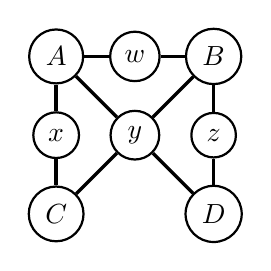
\begin{tikzpicture}
\begin{scope}[every node/.style={circle,thick,draw}]
    \node (C) at (-1,-1) {$C$};
    \node (x) at (-1,0) {$x$};
    \node (A) at (-1,1) {$A$};
    \node (y) at (0,0) {$y$};
    \node (w) at (0,1) {$w$};
    \node (D) at (1,-1) {$D$};
    \node (z) at (1,0) {$z$};
    \node (B) at (1,1) {$B$};
\end{scope}

\begin{scope}[every node/.style={fill=white,circle},
              every edge/.style={draw=black,very thick}]
    \path [-] (A) edge (w);
    \path [-] (A) edge (x);
    \path [-] (A) edge (y);
    \path [-] (B) edge (w);
    \path [-] (B) edge (y);
    \path [-] (B) edge (z);
    \path [-] (C) edge (x);
    \path [-] (C) edge (y);
    \path [-] (D) edge (y);
    \path [-] (D) edge (z);
\end{scope}
\end{tikzpicture}
	\hspace{1cm}
	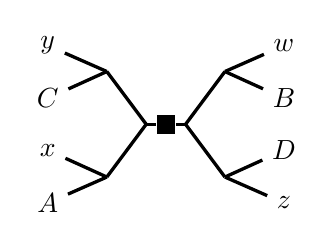
\begin{tikzpicture}
%\begin{scope}[every node/.style={circle,thick,draw}]
    \node (y) at (-1.5,1) {$y$};
    \node (C) at (-1.5,0.33) {$C$};
    \node (x) at (-1.5,-0.33) {$x$};
    \node (A) at (-1.5,-1) {$A$};
    
    \node (w) at (1.5,1) {$w$};
    \node (B) at (1.5,0.33) {$B$};
    \node (D) at (1.5,-0.33) {$D$};
    \node (z) at (1.5,-1) {$z$};
%\end{scope}
    \node (yC) at (-0.75, 0.67) {};
    \node (xA) at (-0.75, -0.67) {};
    \node (wB) at (0.75, 0.67) {};
    \node (zD) at (0.75, -0.67) {};
    
    \node (yCxA) at (-0.25, 0) {};
    \node (wBzD) at (0.25, 0) {};

\begin{scope}[every node/.style={fill=black,rectangle}]
    \node (root) at (0, 0) {};
\end{scope}
    
\begin{scope}[every node/.style={fill=white,circle},
              every edge/.style={draw=black,very thick}]
    \path [-] (y) edge (yC.center);
    \path [-] (C) edge (yC.center);
    \path [-] (x) edge (xA.center);
    \path [-] (A) edge (xA.center);
    \path [-] (w) edge (wB.center);
    \path [-] (B) edge (wB.center);
    \path [-] (z) edge (zD.center);
    \path [-] (D) edge (zD.center);
    
    \path [-] (yC.center) edge (yCxA.center);
    \path [-] (xA.center) edge (yCxA.center);
    \path [-] (wB.center) edge (wBzD.center);
    \path [-] (zD.center) edge (wBzD.center);
    
    \path [-] (yCxA.center) edge (root);
    \path [-] (wBzD.center) edge (root);
\end{scope}
\end{tikzpicture}
	\caption{\label{fig:wmc-example} The tensor network (left) produced by Theorem \ref{thm:wmc-reduction} on $\varphi = (w \lor x \lor \neg y) \land (w \lor y \lor z) \land (\neg x \lor \neg y) \land (\neg y \lor \neg z)$, consisting of 8 tensors and 10 indices. Vertices in this diagram are tensors, while edges indicate that the tensors share an index. The weight function affects the entries of the tensors for $w$, $x$, $y$, and $z$. This tensor network has a contraction tree (right) of max rank 4, but no contraction trees of smaller max rank.}
\end{figure}

Theorem \ref{thm:wmc-reduction} proves that $\func{Reduce}(\varphi,W) = N_{\varphi, W}$ satisfies Assumption 1 in Theorem \ref{thm:alg-correctness}. See Figure \ref{fig:wmc-example} for an example of the reduction. 
This reduction is closely related to the formulation of model counting as the marginalization of a factor graph representing the constraints. 
Unlike the reduction to factor-graph marginalization, which only assigns factors to clauses, we must also assign a tensor to each variable $x$. 
For example, if $x$ has weights $W(x, 0) = W(x,1) = 1$ then the tensor assigned to $x$ is a copy tensor.
This reduction can also be extended beyond OR clauses to other types of constraints, e.g. parity or cardinality constraints.


\section{The Line-Graph Method for Finding Contraction Trees}
\label{sec:tensors:contraction-theory}
The \textbf{Line-Graph} method for finding contraction trees for a tensor network $N$ applies graph-decomposition techniques to a particular graph constructed from $N$. Prior work \cite{MS08} on tensor networks with no free indices constructed a graph from a tensor network where tensors correspond to vertices and indices shared between tensors correspond to edges. In the context of constraint networks \cite{dechter03}, this is analogous to the dual constraint graph (if multiple edges are drawn between constraints with multiple variables in common).

Although tensor networks constructed from weighted model counting instances do not have free indices, we utilize tensor networks with free indices as part of the preprocessing in Section \ref{sec:tensors:preprocessing} and so we need a more general graph construction that can handle free indices. Other works, e.g. \cite{Ying17}, extend the graph construction of \cite{MS08} to tensor networks with free indices by treating free indices as ``half-edges'' (i.e., edges incident to one vertex), but decompositions of such graphs are not well-studied. In order to cleanly extend our decomposition-based analysis to tensor networks with free indices, in this work we instead add an extra vertex incident to all free indices, which we call the \emph{free vertex}. We call the resulting graph the \emph{structure graph} of a tensor network:
\begin{definition}[Structure Graph]\label{def:structure}
	Let $N$ be a tensor network. The \emph{structure graph} of $N$ is the graph $G$ whose 
    vertices are the tensors of $N$ and a fresh vertex $\fv$ (called the \emph{free vertex}) and whose edges are the indices of $N$. Each tensor is incident to its indices, and $\fv$ is incident to all free indices.
    That is, $\V{G} = N \sqcup \{ \fv \}$, $\E{G} = \tnbound{N} \cup \tnfree{N}$, $\vinc{G}{A} = \tdim{A}$ for all $A \in N$, and $\vinc{G}{\fv} = \tnfree{N}$.
\end{definition}

If $N$ has no free indices, the free vertex has no incident edges and the remaining graph is exactly the graph analyzed in prior work. Intuitively, the structure graph of a tensor network $N$ captures how indices are shared by the tensors of $N$. For example, on a CNF formula $\varphi$ Theorem \ref{thm:wmc-reduction} produces a tensor network $N_\varphi$ whose structure graph is exactly the \emph{incidence graph} of $\varphi$. The structure graph of $N$ contains all information needed to compute the max-rank of a contraction-tree of $N$, as formalized in the following lemma.
\begin{lemma} \label{lemma:tcn-equiv-structure}
	Let $N$ be a tensor network with structure graph $G$. If $N' \subseteq N$ is nonempty, then $N'$ is a tensor network and $\tnfree{N'} = \vinc{G}{N'} \cap \vinc{G}{\V{G} \setminus N'}$.
\end{lemma}
\begin{proof}
	$N'$ is a tensor network since $N$ is. Let $\fv$ be the free vertex of $G$.
	An index $i$ is free in $N'$ if and only if $i$ appears in $N'$ and either $i$ is free in $N$ or $i$ also appears in $N \setminus N'$. Thus
    $$\tnfree{N'} = \bigcup_{A \in N'} \tdim{A} \cap \left( \tnfree{N} \cup \bigcup_{B \in N \setminus N'} \tdim{B} \right).$$
	Since $\tdim{A} = \vinc{G}{A}$ for all $A \in N$ and $\tnfree{N} = \vinc{G}{z}$, we conclude that
	$$\tnfree{N'} = \vinc{G}{N'} \cap (\vinc{G}{\fv} \cup \vinc{G}{N \setminus N'}) =  \vinc{G}{N'} \cap \vinc{G}{\V{G} \setminus N'}.$$
\end{proof}



% If $N'$ is a subset of a tensor network $N$, $N'$ is also a subset of vertices in the structure graph of $N$. In this case, the rank of $N'$ is exactly the number of edges in the structure graph of $N$ incident with both a vertex in $N'$ and a vertex in $(N \sqcup \{f\}) \setminus N'$ (where $\fv$ is the free vertex). Thus the structure graph of $N$ contains all the information necessary to compute the rank of a subset of $N$ and thus to compute the max rank of a contraction-tree of $N$.

\subsection{Finding Contraction Trees from Carving Decompositions}
Contraction trees are closely connected to decompositions of the structure graph. In particular, contraction trees of a tensor network correspond to carving decompositions of its structure graph, where max rank corresponds exactly to carving width. This correspondence was first proven for tensor networks with no free indices by de Oliveira Oliveira \cite{de15}. Theorem \ref{thm:contraction-equiv-carving} extends this correspondence to tensor networks with free indices as well:
\begin{theorem}
	\label{thm:contraction-equiv-carving}
	Let $N$ be a tensor network with structure graph $G$ and let $w \in \mathbb{N}$. Then $N$ has a contraction tree of max rank $w$ if and only if $G$ has a carving decomposition of width $w$. Moreover, given one of these objects the other can be constructed in $O(|N|)$ time.
\end{theorem}
%\begin{lemma} \label{lemma:contraction-to-carving}
%	Let $N$ be a tensor network with structure graph $G$. Let $T$ be a contraction tree of $N$ of max-width $w$. Construct $T'$ from $T$ by adding the free vertex $\fv \in \V{G}$ as a leaf and adding an arc from $\fv$ to the root of $T$. Then $T'$ is a carving decomposition of $G$ and $width_c(T) = w$.
%\end{lemma}
\begin{proof}
Let $\fv$ be the free vertex of $G$. First, let $T$ be a contraction tree of $N$ of max-rank $w$. Construct $T'$ from $T$ by adding $\fv$ as a leaf to the root of $T$. 

$T'$ is a carving decomposition of $G$, since $T'$ is an unrooted binary tree with $\Lv{T'} = \Lv{T} \sqcup \{\fv\} = \V{G}$. 
For each $a \in \E{T'}$, removing $a$ from $T'$ produces two connected components, both trees. Let $T_a$ be the connected component that does not contain $\fv$ and note that $T_a$ is a contraction tree for $\Lv{T_a} \subseteq N$. 

This gives us a bijection between $\E{T'}$ and the set of recursive calls of Algorithm \ref{alg:network-contraction}, where each $a \in \E{T'}$ corresponds to the recursive call where $T_a$ is the input contraction tree and $\tntensor{\Lv{T_a}}$ is the output tensor. Thus
\begin{align*}
&width_c(T') = \max_{a \in \E{T'}} \left| \vinc{G}{\Lv{T_a}} \cap \vinc{G}{\V{G} \setminus \Lv{T_a}} \right| = \max_{a \in \E{T'}} \left| \tnfree{\Lv{T_a}} \right| = w
\end{align*}
where the middle equality is given by applying Lemma \ref{lemma:tcn-equiv-structure} with $N' = \Lv{T_a}$.

Conversely, let $S$ be a carving decomposition of $G$ of width $w$. Construct $S'$ from $S$ by removing the leaf $\fv$ (and its incident arc) from $S$. $S'$ is a contraction tree of $N$, since $S$ is a rooted binary tree (whose root is the node previously attached by an arc to $\fv$) and $\Lv{S'} = \Lv{S} \setminus \{\fv\} = N$. Moreover, applying the construction in the first half of the proof produces $S$ and so the max rank of $S'$ is $width_c(S) = w$.
\end{proof}

One corollary of Theorem \ref{thm:contraction-equiv-carving} is that tensor networks with isomorphic structure graphs have contraction trees of equal max rank. This corollary is closely related to Theorem 1 of \cite{EP14}.

Carving decompositions have been studied in several settings. For example, there is an algorithm to find a carving decomposition of minimal width of a planar graph in time cubic in the number of edges \cite{GT08}. It follows that if the structure graph of a tensor network $N$ is planar, one can construct a contraction tree of $N$ of minimal max rank in time $O(|\tnbound{N} \cup \tnfree{N}|^3)$. This may be of interest in domains where problems can be seen as planar or near-planar, e.g. in circuit analysis or infrastructure reliability \cite{MS08,DLVR18}, but most benchmarks we consider in Section \ref{sec:tensors:experiments} do not result in planar structure graphs.

There is limited work on the heuristic construction of ``good'' carving decompositions for non-planar graphs. Instead, we leverage the work behind finding tree decompositions to find carving decompositions and subsequently find contraction trees of small max rank.

\subsection{Finding Contraction Trees from Tree Decompositions}

%In this work, we aim to find ``good'' choices for the rooted binary tree that minimize the running-time and memory usage of Algorithm \ref{alg:network-contraction} on a given tensor contraction network.
%In this work, we make the additional assumption that all dimensions have domains of the same (or similar) size. Thus the max-size of a contraction-tree is entirely characterized by the max rank, and so to find a contraction-tree of small max-size it is equivalent to find a contraction-tree of small max rank.


One technique for join-query optimization \cite{DKV02,MPPV04} focuses on analysis of the \emph{join graph}. The \emph{join graph} of a project-join query consists of all attributes of a database as vertices and all tables in the join as cliques. In this approach, tree decompositions for the join graph of a query are used to find optimal join trees. The analogous technique on factor graphs analyzes the \emph{primal graph} of a factor graph, which consists of all variables as vertices and all factors as cliques. Similarly, tree decompositions of the primal graph can be used to find variable elimination orders \cite{KDLD05}. The graph analogous to join graphs and primal graphs for tensor networks is the \emph{line graph} of the structure graph:
\begin{definition}[Line Graph]
	\label{def:line-graph}
	The \emph{line graph} of a graph $G$ is a graph $\Line{G}$ whose vertices are the edges of $G$, and where the number of edges between each $e,f \in \E{G}$ is $|\einc{G}{e} \cap \einc{G}{f}|$, the number of endpoints shared between $e$ and $f$.
\end{definition}

This technique was applied in the context of tensor networks by Markov and Shi \cite{MS08}, who proved that tree decompositions for $\Line{G}$ (where $G$ is the structure graph of a tensor network $N$) can be transformed into contraction trees for $N$ of small contraction complexity. Specifically, tree decompositions of optimal width $w$ yield contraction trees of contraction complexity $w+1$.

In the following theorem we analyze the max rank of the resulting contraction trees, which has not previously been studied. We present this result as a new relationship between carving width and treewidth:
\begin{theorem} \label{thm:carving-equiv-tree}
	Let $G$ be a graph with $\E{G} \neq \emptyset$. Given a tree decomposition $T$ for $\Line{G}$ of width $w \in \mathbb{N}$, one can construct in polynomial time a carving decomposition for $G$ of width no more than $w+1$.
\end{theorem}

In order to prove this theorem, it is helpful to first state and prove a lemma on simplifying the internal structure of a tree decomposition. In particular, we show that given an edge clique cover of a graph $G$, it is sufficient to only consider tree decompositions whose leaves are labeled only by elements of the edge clique cover.

\begin{lemma}\label{lemma:tree-simplification}
Let $G$ be a graph, let $(T, \chi)$ be a tree decomposition of $G$, and let $A$ be a finite set. If $f: A \rightarrow 2^{\V{G}}$ is a function whose image is an edge clique cover of $G$, then we can construct in polynomial time a tree decomposition $(S, \psi)$ of $G$ and a bijection $g: A \rightarrow \Lv{S}$ with $width_t(S, \psi) \leq width_t(T, \chi)$ and $\psi \circ g = f$.
\end{lemma}
\begin{proof}
Consider an arbitrary $a \in A$ and define $\chi_a: \V{T} \rightarrow 2^{\V{G}}$ by $\chi_a(n) \equiv \chi(n) \cap f(a)$ for all $n \in \V{T}$. Notice that $(T, \chi_a)$ is a tree decomposition of $G \cap f(a)$. Since $f$ is an edge clique cover, $G \cap f(a)$ is a complete graph with $|f(a)|$ vertices and thus has treewidth $|f(a)|-1$. It follows that $width_t(T, \chi_a) \geq |f(a)|-1$. That is, there is some $n_a \in \V{T}$ such that $|\chi_a(n_a)| \geq |f(a)|$. It follows that $\chi_a(n_a) = f(a)$ and so $f(a) \subseteq \chi(n_a)$. Choose an arbitrary arc $b \in \einc{T}{n_a}$ and construct $T'$ from $T$ by attaching a new leaf $\ell_a$ at $b$ (and introducing a new internal node). We can extend $\chi$ into a labeling $\chi': \V{T'} \rightarrow 2^{\E{G}}$ by labeling the new internal node with $\chi(n_a)$ and labeling the new leaf node with $f(a)$. Note that $(T', \chi')$ is still a tree decomposition of $G$ of width $width_t(T, \chi)$, that all labels of leaves of $(T, \chi)$ are still labels of leaves of $(T', \chi')$, and that the new leaf of $(T' \chi')$, namely $\ell_a$, is labeled by $f(a)$.

By repeating this process for every $a \in A$, by induction we produce in polynomial time a tree decomposition $(T', \chi')$ of width $width_t(T, \chi)$. Moreover, define the function $g: A \rightarrow \Lv{T'}$ for all $a \in A$ by $g(a) = \ell_a$ (the new leaf attached at each step). By construction, $\chi' \circ g = f$ (since each $\ell_a$ was labeled by $f(a)$) and moreover $f$ is an injection (since a new leaf was introduced at each step). It remains to make $f$ a bijection by removing leaves of $T'$.

Since $f$ is an edge clique cover, properties (1) and (2) of a tree decomposition can be satisfied purely looking at the nodes of $T'$ in the range of $g$. Moreover, removing leaves of $T'$ cannot falsify property (3) of a tree decomposition. Thus we can repeatedly remove leaves of $T'$ not in the range of $g$ until we eventually reach a tree decomposition $(S, \psi)$ for $G$ whose leaves are exactly the range of $g$. After this process, $g$ is a bijection as a function onto $\Lv{S}$ and $\psi \circ f = \delta_G$. Moreover, since $\psi(\V{S}) \subseteq \chi'(\V{T'})$ it follows that $width_t(S, \psi) \leq width_t(T', \chi') = width_t(T, \chi)$ as desired.
\end{proof}

We now use this lemma to prove Theorem \ref{thm:carving-equiv-tree}.

\begin{proof}
First, observe that the image of $\vincf{G}: \V{G} \rightarrow \E{G}$ is an edge clique cover of $\Line{G}$. It follows by Lemma \ref{lemma:tree-simplification} that we can construct a tree decomposition $(S, \psi)$ of $\Line{G}$ and a bijection $g: \V{G} \rightarrow \Lv{S}$ such that $\psi \circ g = \vincf{G}$ and $width_t(S, \psi) \leq width_t(T, \chi)$.

Construct $T'$ from $S$ by replacing every leaf $\ell \in \Lv{S}$ with $g^{-1}(\ell)$. Since $g$ is a bijection, $\Lv{T'} = \V{G}$ and so $T'$ is a carving decomposition. In order to compute the carving width of $T'$, consider an arbitrary arc $a \in \E{T'}$ and let $C_a$ be an element of the partition of $\V{G}$ defined by removing $a$. 

For every edge $e \in \vinc{G}{C_a} \cap \vinc{G}{\Lv{T'} \setminus C_a}$, there must be vertices $v \in C_a$ and $w \in \Lv{T'} \setminus C_a$ that are both incident to $e$ and so $e \in \vinc{G}{v} \cap \vinc{G}{w}$. Since $\chi \circ g = \vincf{G}$, it follows that $e \in \chi(g(v)) \cap \chi(g(w))$.  Property 3 of tree decompositions implies that $e$ must also be in the label of every node in the path from $g(v)$ to $g(w)$ in $T$; in particular, $e$ must be in the label of both endpoints of $a$.

Thus every element of $\vinc{G}{C_a} \cap \vinc{G}{\Lv{T'} \setminus C_a}$ must be in the label of both endpoints of $a$. It follows that $|\vinc{G}{C_a} \cap \vinc{G}{\Lv{T'} \setminus C_a}| \leq width_t(T, \chi)+1$. Hence $width_c(T') \leq width_t(T, \chi)+1$ as desired.
\end{proof}

An alternative proof of Theorem \ref{thm:carving-equiv-tree} uses Theorem 2.4 of \cite{HW18} to construct a carving decomposition $T'$ of $G$ from $T$ whose vertex congestion is $w+1$. By Lemma 2 of \cite{ACDJPS07}, it follows that the carving width of $T'$ is no more than $w+1$.

Applying Theorem \ref{thm:carving-equiv-tree} when $G$ is the structure graph of a tensor network (together with Theorem \ref{thm:contraction-equiv-carving}) gives us the \textbf{Line-Graph} method, which finds contraction trees by finding tree decompositions of the corresponding line graph. There are several advantages to our new analysis over the analysis of \cite{MS08}: our analysis holds for tensor networks with free indices, and we analyze the max rank of contraction trees instead of the contraction complexity. Although the contraction complexity (and, for factor graphs, the width of the elimination order) is equal to one plus the width of the used tree decomposition, the max rank is smaller on some graphs; see the appendix for an experimental analysis of this.
\section{The Factor-Tree Method for Finding Contraction Trees}
\label{sec:preprocessing}
Approaches to tensor-network contraction that do not modify the input tensor network (e.g., \textbf{LG}) are inherently limited by the ranks of the input tensors. If a tensor network has a rank $r$ tensor, then all contraction trees have max rank of at least $r$. This is a problem for tensor networks with high-rank tensors. 

One example of tensor networks that may contain high-rank tensors are the networks obtained by the reduction from model counting. The tensor network produced from a formula $\varphi$ contains a tensor representing each variable $x$, where the rank of this tensor is the number of appearances of $x$ in $\varphi$ (e.g., the rank $4$ tensor for $y$ in Figure \ref{fig:wmc-example}). For many benchmarks, where a single variable might appear tens or even hundreds of times, this reduction will therefore produce tensor networks containing tensors of infeasibly-high rank. Reductions exist from model counting on arbitrary formulas to model counting on formulas where the number of appearances of each variables is small. However, existing reductions do not consider the carving width of the resulting incidence graph and so often do not significantly improve the max-rank of available contraction trees. 

We introduce here a novel method \textbf{Factor-Tree} that avoids this barrier by preprocessing the input tensor network. Our insight is that a tree decomposition for the incidence graph of $\varphi$ can be used as a guide to introduce new variables in a principled way, so that the resulting tensor network has good contraction trees. In the language of tensors, introducing new variables corresponds to \emph{factoring}: replacing each high-rank tensor $A$ with a tensor network $N_A$ of low-rank tensors that contracts to $A$. The key idea of \textbf{FT}, then, is to use a tree decomposition for the structure graph to factor high-rank tensors.

We state this new result as Theorem \ref{thm:factorable-tree}. Since not all tensors can be factored in the ways that we require for this theorem and for \textbf{FT}, we first characterize the required property: that every tensor is factorable as an arbitrary tree of tensors:

% In fact, we can generalize this result to a wider class of tensor networks. To use a tree decomposition as a guide to simplify a tensor network we ultimately require that we can identify each tensor with a tensor network whose structure graph (excluding the free vertex) is an arbitrary tree. We call this property \emph{tree factorable}:

% We demonstrate an algorithm to find in polynomial time a tensor network, consisting only of rank 3 tensors, whose contraction is the model count of $F$. Moreover, we prove that the resulting tensor network has a good contraction tree if the guiding tree decomposition has small width.
%Instead of directly proving these claims (which are ultimately a corollary of Theorem \ref{thm:factorable-tree}), we generalize this result to a wider class of tensor networks. 

\begin{definition} \label{def:tree-factorable}
A tensor $A$ is \emph{tree factorable} if, for every tree $T$ whose leaves are $\tdim{A}$ (called a \emph{dimension tree} of $A$), there is a tensor network $N_A$ and a bijection $g_A: \V{T} \rightarrow N_A$ s.t.
\begin{enumerate}
\item $A$ is the contraction of $N_A$,
\item $g_A$ is an isomorphism between $T$ and the structure graph of $N_A$ with the free vertex (and incident edges) removed,
\item for every index $i$ of $A$, $i$ is an index of $g_A(i)$, and
\item for some index $i$ of $A$, the bond dimension of $N_A$ is no bigger than $|\domain{i}|$. % $\max_{i \in \tnbound{N}} |\domain{i}| \leq \max_{i \in \tdim{A}} |\domain{i}|$.
\end{enumerate}
\end{definition}
All tensors in the reduction of Theorem \ref{thm:wmc-reduction} from weighted model counting to tensor networks are tree factorable. A tensor network $N_A$ that satisfies properties 1, 2, and 3 of Definition \ref{def:tree-factorable} for some tree is called a \emph{Hierarchical Tucker representation} of $A$ \cite{Grasedyck10}. Property 4 ensures the result of Theorem \ref{thm:factorable-tree} has small bond dimension.

% In \cite{Grasedyck10}, a tree $T$ as in Definition \ref{def:tree-factorable} is called a \emph{dimension tree} of the tensor $A$, and a tensor network $N$ that satisfies properties 1, 2, and 3 for a given dimension tree of $A$ is called a \emph{Hierarchical Tucker representation} of $A$. For every tensor $A$ and dimension tree, a hierarchical Tucker representation of $A$ trivially exists with bond dimension $|\domain{A}|$, but a representation may not exist with smaller bond dimension. Limiting the bond dimension in property 4 ensures that the tensor networks we produce in Theorem \ref{thm:factorable-tree} also have small bond dimension.

We now state the main result of this section, which allows us to use a tree decomposition for the structure graph of a tensor network (containing only tree factorable tensors) to factor each tensor in the network and find a contraction tree of low max rank for the resulting network:
\begin{figure}[t]
	\centering
	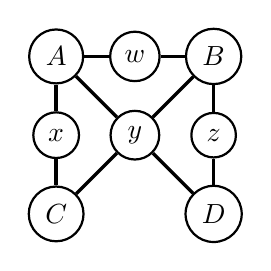
\begin{tikzpicture}
\begin{scope}[every node/.style={circle,thick,draw}]
    \node (C) at (-1,-1) {$C$};
    \node (x) at (-1,0) {$x$};
    \node (A) at (-1,1) {$A$};
    \node (y) at (0,0) {$y$};
    \node (w) at (0,1) {$w$};
    \node (D) at (1,-1) {$D$};
    \node (z) at (1,0) {$z$};
    \node (B) at (1,1) {$B$};
\end{scope}

\begin{scope}[every node/.style={fill=white,circle},
              every edge/.style={draw=black,very thick}]
    \path [-] (A) edge (w);
    \path [-] (A) edge (x);
    \path [-] (A) edge (y);
    \path [-] (B) edge (w);
    \path [-] (B) edge (y);
    \path [-] (B) edge (z);
    \path [-] (C) edge (x);
    \path [-] (C) edge (y);
    \path [-] (D) edge (y);
    \path [-] (D) edge (z);
\end{scope}
\end{tikzpicture}
	\hspace{1cm}
	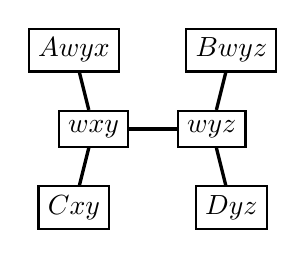
\begin{tikzpicture}
\begin{scope}[every node/.style={rectangle,thick,draw}]
    \node (1) at (-1,1) {$Awyx$};
    \node (2) at (-1,-1) {$Cxy$};
    \node (3) at (-0.75,0) {$wxy$};
    \node (4) at (0.75,0) {$wyz$};
    
    \node (5) at (1,1) {$Bwyz$};
    \node (6) at (1,-1) {$Dyz$};
\end{scope}

\begin{scope}[every node/.style={fill=white,circle},
              every edge/.style={draw=black,very thick}]
    \path [-] (1) edge (3);
    \path [-] (2) edge (3);
    \path [-] (3) edge (4);
    \path [-] (4) edge (5);
    \path [-] (4) edge (6);
\end{scope}
\end{tikzpicture}
	\hspace{1cm}
	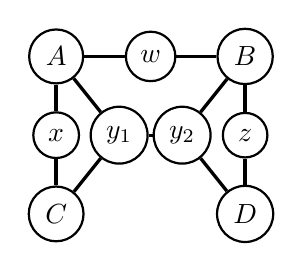
\begin{tikzpicture}
\begin{scope}[every node/.style={circle,thick,draw}]
    \node (C) at (-1.2,-1) {$C$};
    \node (x) at (-1.2,0) {$x$};
    \node (A) at (-1.2,1) {$A$};
    \node (y1) at (-0.4,0) {$y_1$};
    \node (y2) at (0.4,0) {$y_2$};
    \node (w) at (0,1) {$w$};
    \node (D) at (1.2,-1) {$D$};
    \node (z) at (1.2,0) {$z$};
    \node (B) at (1.2,1) {$B$};
\end{scope}

\begin{scope}[every node/.style={fill=white,circle},
              every edge/.style={draw=black,very thick}]
    \path [-] (A) edge (w);
    \path [-] (A) edge (x);
    \path [-] (A) edge (y1);
    \path [-] (B) edge (w);
    \path [-] (B) edge (y2);
    \path [-] (B) edge (z);
    \path [-] (y1) edge (y2);
    \path [-] (C) edge (x);
    \path [-] (C) edge (y1);
    \path [-] (D) edge (y2);
    \path [-] (D) edge (z);
\end{scope}
\end{tikzpicture}
	\caption{\label{fig:factor-example} When FT is run on the shown initial tensor network (left) using the shown tree decomposition (middle), \textbf{FT} produces a factored tensor network (right). Tensors of rank 3 or smaller are unchanged, and the tensor for $y$ is factored into two tensors, $y_1$ and $y_2$, each of rank 3. The factored tensor network has a contraction tree of max rank 3 while the initial tensor network only has contraction trees of max rank 4 or higher.}
\end{figure}

\begin{theorem} \label{thm:factorable-tree}
Let $N$ be a tensor network of tree-factorable tensors such that $|\tnfree{N}| \leq 3$ and the structure graph of $N$ has a tree decomposition of width $w \geq 1$.

Then for each $A \in N$ there is a tensor network $N_A$ whose contraction is $A$ that consists only of rank 3 or smaller tensors. Moreover, the disjoint union of these networks, $M = \cup_{A \in N} N_A$, is a tensor network that contracts to $\tntensor{N}$, has the same bond dimension as $N$, and has a contraction tree of max rank no larger than $\ceil{4(w+1)/3}$.
\end{theorem}
\begin{proof}
The proof proceeds in five steps: (1) compute the factored tensor network $M$, (2) construct a graph $H$ that is a simplified version of the structure graph of $M$, (3) construct a carving decomposition $S$ of $H$, (4) bound the width of $S$, and (5) use $S$ to find a contraction tree for $M$. Working with $H$ instead of directly working with the structure graph of $M$ allows us to cleanly handle tensor networks with free indices.

\textbf{Part 1: Factoring the network.}
Let $G$ be the structure graph of $N$ with all degree 0 vertices removed; $G$ must also have a tree decomposition of width $w$. Moreover, the image of $\eincf{G}: \E{G} \rightarrow 2^{\V{G}}$ is an edge clique cover of $G$. Thus using Lemma \ref{lemma:tree-simplification} we can construct a tree decomposition $(T, \chi)$ of $G$ and a bijection $g: \E{G} \rightarrow \Lv{T}$ such that $\chi \circ g = \eincf{G}$ and $width_t(T, \chi) \leq w$.

Next, for each $v \in \V{G}$, define $T_v$ to be the smallest connected component of $T$ containing $\{g(i) ~:~i \in \vinc{H}{v} \}$. Consider each $A \in N$. If $\tnfree{A} = \emptyset$, let $N_A = \{A\}$; thus $\tntensor{N_A} = A$ and the tensor of $N_A$ has rank 0. Otherwise, observe that $T_A$ is a dimension tree of $A$. We can therefore factor $A$ with $T_A$ using Definition \ref{def:tree-factorable} to get a tensor network $N_A$ whose contraction is $A$ and a bijection $g_A: \V{T_A} \rightarrow N_A$. Moreover, every node of $T_A$ has degree 3 or smaller and so, by Definition \ref{def:tree-factorable}, $N_A$ consists only of rank 3 or smaller tensors.

Define $M = \cup_{A \in N} N_A$ and let $G'$ be the structure graph of $M$ with free vertex $\fv'$. The remainder of the proof is devoted to bounding the carving width of $G'$.

\textbf{Part 2: Constructing a simplified structure graph of $M$.} In order to easily characterize $G'$, we define a new, closely-related graph $H$ by taking a copy of $T_v$ for each $v \in \V{G}$ and connecting these copies where indicated by $g$. Formally, the vertices of $H$ are $\{(v, n) : v \in \V{G}, n \in \V{T_v}\}$. For every $v \in \V{G}$ and every arc in $T$ with endpoints $n, m \in \V{T_v}$, we add an edge between $(v, n)$ and $(v, m)$. Moreover, for each $e \in \E{G}$ incident to $v, w \in \V{G}$, we add an edge between $(v, g(e))$ and $(w, g(e))$. 

We will prove in Part 5 that the carving width of $G'$ is bounded from above by the carving width of $H$. We therefore focus in Part 3 and Part 4 on bounding the carving width of $H$. It is helpful for this to define the two projections $\pi_G : \V{H} \rightarrow \V{G}$ and $\pi_T : \V{H} \rightarrow \V{T}$ that indicate respectively the first or second component of a vertex of $H$. 
% For each $v \in \V{G}$, define $H_v = \pi_G^{-1}(v)$. Thus the sets $H_v$ form a partition of $\V{H}$. 

% This ensures that $H \cap H_v$ is isomorphic to $T_v$ and so $H \cap H_v$ is a tree with $|\vinc{G}{v}|$ leaves.

% The map $f: \E{G} \rightarrow \E{H}$ constructed in this way is an injection and satisfies property 3 above. Moreover, since $g(\vinc{G}{v})$ is exactly the leaves of $T_v$, each leaf $\ell \in \Lv{H \cap H_v}$ is incident to exactly one edge in the range of $f$, namely $f(g^{-1}(\ell))$.

\begin{figure}[t]
	\centering
	%\begin{tikzpicture}
\begin{scope}[every node/.style={fill, circle, inner sep=0pt, outer sep=0, minimum size=5pt}]
    \node[label={[xshift=5pt]$n$}] (n) at (0, 0) {};
\end{scope}

\draw[thick] (n) -- (0, 2) node [midway, left] {$a$};
\draw[thick] (n) -- (-1.73, -1) node [midway, above] {$b$};
\draw[thick] (n) -- (1.73, -1) node [midway, above] {$c$};
\end{tikzpicture}
	%\hspace{1cm}
	\begin{tikzpicture}
% Center node
\node[fill, circle, inner sep=0pt, outer sep=0, minimum size=5pt, label={[xshift=8pt, yshift=-5pt]$y_n$}] (yn) at (0, 0) {};

% Minor nodes
\begin{scope}[every node/.style={fill, circle, inner sep=0pt, outer sep=0, minimum size=3pt}]
    \draw[thick] (yn) -- node[pos=0.75, label=right:{$z_{n,a}$}, minimum size=5pt] (zna) {} 
    node[pos=0.525] (Ina1) {} node[pos=0.375] (Ina2) {} node[pos=0.225] (Ina3) {} (0,2);
    \node[left=0.5 of Ina1] (Hna1) {};
    \node[left=0.5 of Ina2] (Hna2) {};
    \node[left=0.5 of Ina3] (Hna3) {};
    
    \draw[thick] (yn) -- node[pos=0.75, label={[xshift=-5pt,yshift=-5pt]$z_{n,b}$}, minimum size=5pt] (znb) {}
    node[pos=0.525] (Inb1) {} node[pos=0.375] (Inb2) {} node[pos=0.225] (Inb3) {} (-1.73, -1);
    \node[below right=0.25 and 0.1 of Inb1] (Hnb1) {};
    \node[below right=0.25 and 0.1 of Inb2] (Hnb2) {};
    \node[below right=0.25 and 0.1 of Inb3] (Hnb3) {};
    
    \draw[thick] (yn) -- node[pos=0.75, label={[xshift=5pt,yshift=-5pt]$z_{n,c}$}, minimum size=5pt] (znc) {}
    node[pos=0.525] (Inc1) {} node[pos=0.375] (Inc2) {} node[pos=0.225] (Inc3) {} (1.73, -1);
    \node[below left=0.25 and 0.1 of Inc1] (Hnc1) {};
    \node[below left=0.25 and 0.1 of Inc2] (Hnc2) {};
    \node[below left=0.25 and 0.1 of Inc3] (Hnc3) {};
    
    % \node[left=5 of zna, label=right:{$z_{\ell,a}$}, minimum size=5pt] (zla) {};
    % \node[left=5 of Ina1] (Ila1) {};
    % \node[left=5 of Ina2] (Ila2) {};
    % \node[left=5 of Ina3] (Ila3) {};
    % \node[left=5 of Hna1] (Hla1) {};
    % \node[left=5 of Hna2] (Hla2) {};
    % \node[left=5 of Hna3] (Hla3) {};
    
    \draw[thick] (-3, 0.52) -- node[pos=0.6825, label=right:{$z_{\ell,a}$}, minimum size=5pt] (zna) {}
    node[pos=0.39] (Ila1) {} node[pos=0.195] (Ila2) {} node[pos=0] (Ila3) {} (-3,2);
    \node[left=0.5 of Ila1] (Hla1) {};
    \node[left=0.5 of Ila2] (Hla2) {};
    \node[left=0.5 of Ila3] (Hla3) {};
\end{scope}

% \node at (zna) [above right] {$y_n$};
%\draw[thick] (yn) -- (0, 2);
%\draw[thick] (yn) -- (-1.73, -1);
%\draw[thick] (yn) -- (1.73, -1);

\draw[thick] (Ina1) -- (Hna1);
\draw[thick] (Ina2) -- (Hna2);
\draw[thick] (Ina3) -- (Hna3);
\draw[decoration={brace,raise=3pt},decorate] (Ina1) -- node[right=4pt] {$I_{n,a}$} (Ina3);
\draw[decoration={brace,mirror,raise=3pt},decorate] (Hna1) -- node[left=4pt] {$H_{n,a}$} (Hna3);

\draw[thick] (Inb1) -- (Hnb1);
\draw[thick] (Inb2) -- (Hnb2);
\draw[thick] (Inb3) -- (Hnb3);
\draw[decoration={brace,raise=3pt},decorate] (Inb1) -- node[above left=1pt and 1pt] {$I_{n,b}$} (Inb3);
\draw[decoration={brace,mirror,raise=3pt},decorate] (Hnb1) -- node[below=6pt] {$H_{n,b}$} (Hnb3);

\draw[thick] (Inc1) -- (Hnc1);
\draw[thick] (Inc2) -- (Hnc2);
\draw[thick] (Inc3) -- (Hnc3);
\draw[decoration={brace,mirror,raise=3pt},decorate] (Inc1) -- node[above right=1pt and 1pt] {$I_{n,c}$} (Inc3);
\draw[decoration={brace,raise=3pt},decorate] (Hnc1) -- node[below=6pt] {$H_{n,c}$} (Hnc3);


\draw[thick] (Ila1) -- (Hla1);
\draw[thick] (Ila2) -- (Hla2);
\draw[thick] (Ila3) -- (Hla3);
\draw[decoration={brace,raise=3pt},decorate] (Ila1) -- node[right=4pt] {$I_{\ell,a}$} (Ila3);
\draw[decoration={brace,mirror,raise=3pt},decorate] (Hla1) -- node[left=4pt] {$H_{\ell,a}$} (Hla3);
\end{tikzpicture}
	\caption{\label{fig:factor-carving-construction} The central construction in Part 3 of Theorem \ref{thm:factorable-tree} of a carving decomposition $S$ from an input tree decomposition $(T, \chi)$. Each leaf $\ell$ of $T$ (with incident arc $a$) is replaced by the left construction in $S$. Each internal node $n$ of $T$ (with incident arcs $a$, $b$, and $c$) is replaced by the right construction in $S$. If nodes $m$ and $n$ are connected by arc $a$ in $T$, then nodes $z_{m,a}$ and $z_{n,a}$ are connected in $S$.}
\end{figure}

\textbf{Part 3. Constructing a carving decomposition $S$ of $H$.}
The idea of the construction is, for each $n \in \V{T}$, to attach the elements of $\pi_T^{-1}(n)$ as leaves along arcs incident to $n$. See Figure \ref{fig:factor-carving-construction} for an overview of the construction.

Consider an arbitrary node $n \in \V{T}$. If $n$ is a leaf node with incident arc $a \in \vinc{T}{n}$, define $H_{n,a} = \pi_T^{-1}(n)$. If $n$ is an internal node with incident arcs $a,b,c \in \vinc{T}{n}$, arbitrarily partition $\pi_T^{-1}(n)$ into three equally-sized sets $B_1$, $B_2$, and $B_3$ and define $H_{n,a} = B_1$, $H_{n,b} = B_2$, and $H_{n,c} = B_3$ (note that $T$ is a binary tree and so $n$ has exactly three incident arcs). Observe that, in either case, $\{H_{n,a} : n \in \V{T}, a \in \vinc{T}{n}\}$ is a partition of $\pi_T^{-1}(n)$ and thus is a partition of $\V{H}$. 
% To do this, for every leaf node $\ell \in \Lv{T}$ with incident arc $a \in \vinc{T}{\ell}$ define $H_{\ell, a} = \pi_T^{-1}(\ell)$. For every non-leaf node $n \in \V{T} \setminus \Lv{T}$ partition $\pi_T^{-1}(n)$ into three equally-sized sets and denote each set by $H_{n,a}$ for each of the three $a \in \vinc{T}{n}$. Observe that $\{H_{n,a} : n \in \V{T}, a \in \vinc{T}{n}\}$ is a partition of $\V{H}$. 

We use this to construct a carving decomposition $S$ from $T$ by adding each element of $H_{n,a}$ as a leaf along the arc $a$. Formally, let $x_v$ denote a fresh vertex for each $v \in \V{H}$, let $y_n$ denote a fresh vertex for each $n \in \V{T}$, and let $z_{n,a}$ denote a fresh vertex for each $n \in \V{T}$ and $a \in \vinc{T}{n}$. Define $\V{S}$ to be the union of $\V{H}$ with the set of these free vertices. 

We add an arc between $v$ and $x_v$ for every $v \in \V{H}$. Moreover, for every $a \in \E{T}$ with endpoints $o, p \in \einc{T}{a}$ add an arc between $z_{o,a}$ and $z_{p,a}$. For every $n \in \V{T}$ and incident arc $a \in \vinc{T}{n}$, construct an arbitrary sequence $I_{n,a}$ from $\{x_v : v \in H_{n,a}\}$. If $H_{n,a} = \emptyset$ then add an arc between $y_n$ and $z_{n,a}$. Otherwise, add arcs between $y_n$ and the first element of $I$, between consecutive elements of $I_{n,a}$, and between the last element of $I_{n,a}$ and $z_{n,a}$. 

Finally, remove the previous leaves of $T$ from $S$. The resulting tree $S$ is a carving decomposition of $H$, since we have added all vertices of $H$ as leaves and removed the previous leaves of $T$.

\textbf{Part 4: Computing the width of $S$.} In this part, we separately bound the width of the partition induced by each of the three kinds of arcs in $S$.

First, consider an arc $d$ between some $v \in \V{H}$ and $x_v$. Since all vertices of $H$ are degree 3 or smaller, $d$ defines a partition of width at most $3 \leq \ceil{4(w+1)/3}$.

Next, consider an arc $e_a$ between $z_{o,a}$ and $z_{p,a}$ for some arc $a \in \E{T}$ with endpoints $o, p \in \einc{T}{a}$.
Observe that removing $a$ from $T$ defines a partition $\{B_o, B_p\}$ of $\V{T}$, denoted so that $o \in B_o$ and $p \in B_p$. Then removing $e_a$ from $S$ defines the partition $\{ \pi_T^{-1}(B_o), \pi_T^{-1}(B_p) \}$ of $\Lv{S}$. By construction of $H$, all edges between $\pi_T^{-1}(B_o)$ and $\pi_T^{-1}(B_p)$ are between $\pi_T^{-1}(o)$ and $\pi_T^{-1}(p)$. Since $\pi_G(\pi_T^{-1}(o)) \subseteq \chi(o)$, $\pi_G(\pi_T^{-1}(o)) \subseteq \chi(p)$, and $\pi_G$ is an injection on $\pi_T^{-1}(n)$ for all $n \in \V{T}$), it follows that the partition defined by $e_a$ has width no larger than $|\chi(o) \cap \chi(p)| \leq w+1$. 

Finally, consider an arc $f$ added as one of the sequence of $|H_{n,a}|+1$ arcs between $y_n$, $I_{n,a}$, and $z_{n,a}$ for some $n \in \V{T}$ and $a \in \vinc{T}{n}$. Some elements of $H_{n,a}$ have changed blocks from the partition defined by $e_a$. Each vertex of degree 2 that changes blocks does not affect the width of the partition, but each vertex of degree 3 that changes blocks increases the width by 1. There are at most $|H_{n,a}| \leq \ceil{(w+1)/3}$ elements of degree 3 added as leaves between $y_n$ and $z_{n,a}$. Thus the partition defined by $f$ has width at most $w + 1 + \ceil{(w+1)/3} = \ceil{4(w+1)/3}$.

It follows that the width of $S$ is at most $\ceil{4(w+1)/3}$.

\textbf{Part 5: Bounding the max-rank of $M$.} Let $\fv$ be the free vertex of the structure graph of $N$. We first construct a new graph $H'$ from $H$ by, if $\tnfree{N} \neq \emptyset$, contracting all vertices in $\pi_G^{-1}(\fv)$ to a single vertex $\fv$. If $\tnfree{N} = \emptyset$, instead add $\fv$ as a fresh degree 0 vertex to $H'$. Moreover, for all $A \in N$ with $\tdim{A} = \emptyset$ add $A$ as a degree 0 vertex to $H'$. 

Note that adding degree 0 vertices to a graph does not affect the carving width. Moreover, since $|\tnfree{N}| \leq 3$ all vertices (except at most one) of $\pi_G^{-1}(\fv)$ are degree 2 or smaller. It follows that contracting $\pi_G^{-1}(\fv)$ does not increase the carving width. Thus the carving width of $H'$ is at most $\ceil{4(w+1)/3}$.

Moreover, $H'$ and $G'$ are isomorphic. To prove this, define an isomorphism $\phi: \V{H'} \rightarrow \V{G'}$ between $H'$ and $G'$ by, for all $v \in \V{H'}$:
$$\phi(v) \equiv \begin{cases}v&\text{if}~v \in N~\text{and}~\tdim{v}=\emptyset\\\fv'&v=\fv\\g_{\pi_G(v)}(\pi_T(v))&\text{if}~v \in \V{H}~\text{and}~\pi_G(v) \in N\end{cases}$$
$\phi$ is indeed an isomorphism between $H'$ and $G'$ because the functions $g_A$ are all isomorphisms and because an edge exists between $\pi_G^{-1}(v)$ and $\pi_G^{-1}(w)$ for $v, w \in \V{G}$ if and only if there is an edge between $v$ and $w$ in $G$. Thus the carving width of $G'$ is at most $\ceil{4(w+1)/3}$. By Theorem \ref{thm:contraction-equiv-carving}, then, $M$ has a contraction tree of max rank no larger than $\ceil{4(w+1)/3}$.
\hfill$\square$
\end{proof}

The general idea of using a tree decomposition of a graph to split high-degree nodes was previously used by Markov and Shi \cite{MS11} and in the context of constraint satisfaction by Samer and Szeider \cite{SS10_2}. Both of these works focus on minimizing the treewidth of the factored graph instead of the max-rank. Translated to tensor networks (as done in Lemma 3 of \cite{oliveira18}), their constructions produce a factored network $N'$ with structure graph $G$ that satisfies all requirements of Theorem \ref{thm:factorable-tree} except with a bound of $w+1$ on the treewidth of $G$ in place of the bound on max-rank. Since the treewidth of $\Line{G}$ plus 1 is bounded by the product of the maximum degree of $G$ (namely 3) and the treewidth of $G$ plus 1 \cite{MS08}, we can then use \textbf{LG} to produce a contraction tree for $N'$ of max rank no larger than $3(w+2)$. Theorem \ref{thm:factorable-tree} thus gives an improvement on max-rank over these prior works from $3(w+2)$ to $\ceil{4(w+1)/3}$.

% who used tree decompositions of the incidence graph of a CSP to construct an equisatisfiable CSP of identical incidence treewidth in which no variable occurs more than 3 times. Translated to the context of tensor networks and generalized to tree-factorable tensors, their analysis produces a factored tensor network $N'$ that satisfies all requirements of Theorem \ref{thm:factorable-tree} but with a bound of $w$ on the incidence treewidth instead of our bound on max-rank.

%\begin{theorem} \label{thm:factorable-tree}
%Let $N$ be a tensor network of tree-factorable tensors such that $|\tnfree{N}| \leq 3$ and the structure graph of $N$ has a tree decomposition $T$ of width $w$.

%Then for each $A \in N$ there is a tensor network $N_A$ whose contraction is $A$ that consists only of rank 3 or smaller tensors. Moreover, the disjoint union of these networks, $N' = \cup_{A \in N} N_A$, is a tensor network that contracts to $\tntensor{N}$, has the same bond dimension as $N$, and has a structure graph with a tree decomposition of width $w$.
%\end{theorem}


The construction of Theorem \ref{thm:factorable-tree} gives us the \textbf{Factor-Tree} method, which uses tree decompositions of the structure graph to preprocess the tensor network and factor high-rank tensors. See Figure \ref{fig:factor-example} for an example of the preprocessing. We show in Section \ref{sec:experiments:cachet} that \textbf{FT} can significantly improve the quality of the contraction tree on benchmarks with high-rank tensors.
\section{Implementation and Evaluation} \label{sec:tensors:experiments}
We aim to answer the following experimental research questions:
\begin{enumerate}
    \item[(RQ1)] Are tensor-network-based approaches competitive with existing state-of-the-art unweighted model counters?
    \item[(RQ2)] Are tensor-network-based approaches competitive with existing state-of-the-art weighted model counters?
    \item[(RQ3)] What are the structural properties of benchmarks for which the tensor-network-based approaches perform well?
\end{enumerate}

To answer these questions, we implement Algorithm 2 in \tool{TensorOrder}, a new tool for weighted model counting using tensor networks. \tool{TensorOrder} can be configured to find contraction trees using existing planning methods -- \textbf{greedy} (using a greedy algorithm), \textbf{metis} (using graph partitioning), and \textbf{GN} (using community structure detection) \cite{KCMR18}-- or planning methods presented in this paper-- \textbf{LG} (Section \ref{sec:tensors:contraction-theory}) and \textbf{FT} (Section \ref{sec:tensors:preprocessing}). Implementation details appear in Section \ref{sec:tensors:experiments:implementation}.

To answer RQ1, in Section \ref{sec:tensors:experiments:cubic} we compare \tool{TensorOrder} with existing state-of-the-art tools for unweighted model counting (\tool{dynQBF} \cite{CW16}, \tool{dynasp} \cite{FHMW17}, \tool{SharpSAT} \cite{Thurley2006}, \tool{cachet} \cite{SBK05}, \tool{miniC2D} \cite{OD15} and \tool{d4} \cite{LM17}) on formulas that count the number of vertex covers of randomly-generated cubic graphs \cite{KCMR18}. Note \tool{dynQBF} and \tool{dynasp} are solvers from related domains (that can be used as tools for unweighted model counting) that also use tree decompositions.

To answer RQ2, in Section \ref{sec:tensors:experiments:cachet} we compare \tool{TensorOrder} with existing state-of-the-art tools for weighted model counting (\tool{cachet} \cite{SBK05}, \tool{miniC2D} \cite{OD15} and \tool{d4} \cite{LM17}) on formulas whose weighted count corresponds to exact inference on Bayesian networks \cite{SBK05}. Note that the other tools (\tool{dynQBF}, \tool{dynasp}, and \tool{SharpSAT}) cannot perform weighted model counting.

% We use \tool{TensorOrder} to compare tensor-based methods with existing state-of-the-art tools for weighted model counting: \tool{cachet} \cite{SBK05}, \tool{miniC2D} \cite{OD15} and \tool{d4} \cite{LM17}. %Note that \tool{d4} requires a d-DNNF reasoner to perform weighted model counting; we use \cite{CDLL18}. 
% We also compare with \tool{dynQBF} \cite{CW16}, \tool{dynasp} \cite{FHMW17} and \tool{SharpSAT} \cite{Thurley2006} when the benchmarks are unweighted. Note \tool{dynQBF} and \tool{dynasp} are solvers from related domains (that can be used as model counters) that also use tree decompositions.

% We then compare our tensor-based algorithms for weighted model counting against state-of-the-art weighted model counters and against existing tensor-based algorithms. We demonstrate that our tensor-based algorithms are useful as part of a portfolio of weighted model counters. 

% We compare \tool{TensorOrder} on two sets of existing benchmarks. First, in Section \ref{sec:tensors:experiments:cubic} we compare on formulas that count the number of vertex covers of randomly-generated cubic graphs \cite{KCMR18}. Second, in Section \ref{sec:tensors:experiments:cachet} we compare 
To answer RQ3, we compute upper bounds on the treewidth and carving width of these benchmarks. We run each of three heuristic tree decomposition solvers (\pkg{Tamaki} \cite{Tamaki17}, \pkg{FlowCutter} \cite{HS18}, and \pkg{htd} \cite{AMW17}) on each benchmark with a timeout of 1000 seconds: once on the structure graph $G$ corresponding to the benchmark, and once on $\Line{G}$. The minimal width of all produced tree decompositions for $G$ (resp. $\Line{G}$) is an upper bound for the treewidth of $G$ (resp. $\Line{G}$). The minimal max rank of the contraction trees produced by running \textbf{LG} (resp. \textbf{FT}) on each tree decomposition of $\Line{G}$ (resp. $G$) is an upper bound for the carving width of $G$ (resp. $G$ after \text{FT}-preprocessing).

Each experiment was run in a high-performance cluster (Linux kernel 2.6.32) using a single 2.80 GHz core of an Intel Xeon X5660 CPU and 48 GB RAM. We provide all code, benchmarks, and detailed data of benchmark runs at \url{https://github.com/vardigroup/TensorOrder}.

% \paragraph{Experimental Methodology}
% To evaluate runtime performance, we run each tool once on each benchmark with a timeout of 1000 seconds and record the wall-clock time taken. For \tool{TensorOrder}, recorded times include all of Algorithm \ref{alg:wmc} (and, specifically, include the time of the underlying tree-decomposition solver).



% We then use these tree decompositions to compute upper bounds on the treewidth of $G$ (the minimal width of all found tree decompositions for $G$), the treewidth of $\Line{G}$ (the minimal width of all found tree decompositions for $\Line{G}$), the carving width of $G$ (the minimal max rank of all contraction trees produced by running \textbf{LG} on tree decompositions of $\Line{G}$), and the carving width of $G$ after \textbf{FT}-preprocessing (the minimal max rank of all contraction trees produced by running \textbf{FT} on tree decompositions of $\Line{G}$).

% \begin{enumerate}
%     \item the treewidth of $G$ by taking the minimum width amongst all discovered tree decompositions for $G$,
%     \item the treewidth of $\Line{G}$ by taking the minimum width amongst all discovered tree decompositions for $\Line{G}$,
%     \item the carving width of $G$ by taking the minimum width amongst all contraction trees produced by running \textbf{LG} on each tree decomposition of $\Line{G}$, and
%     \item the carving width of $G$ after \textbf{FT}-preprocessing by taking the minimum width amongst all contraction trees produced by running \textbf{FT} on each tree decomposition of $G$.
% \end{enumerate}

% compute an upper bound for the treewidth of $G$ (resp. $\Line{G}$) by taking the minimum width amongst all discovered tree decompositions for $G$ (resp. $\Line{G}$). Similarly, we compute an upper bound for the carving width of $G$ by taking the minimum width amongst all contraction trees produced by running \textbf{LG} on each tree decomposition of $\Line{G}$.


% We then record the width of the best tree decomposition found amongst all tree-decomposition solvers. We also 

% We also evaluate the structural properties of these benchmarks by performing an experimental comparison of treewidth and carving width of the incidence. For each benchmark with corresponding incidence graph $G$, we run each of the three heuristic tree decomposition solvers \tool{Tamaki}, \tool{FlowCutter}, and \tool{htd} for 1000 seconds on $G$ and $\Line{G}$. We then record the width of the best tree decomposition found amongst all tree-decomposition solvers. On each tree decomposition for $\Line{G}$ found by the solvers, we use \textbf{LG} to compute the corresponding carving decomposition of $G$ and recorded the smallest width found amongst all decompositions. Similarly, on each tree decomposition for $G$ found by the solvers, we use \textbf{FT} to compute the corresponding carving decomposition of the preprocessed graph and recorded the smallest width found amongst all decompositions. 

\begin{figure}
	\centering
	%% Creator: Matplotlib, PGF backend
%%
%% To include the figure in your LaTeX document, write
%%   \input{<filename>.pgf}
%%
%% Make sure the required packages are loaded in your preamble
%%   \usepackage{pgf}
%%
%% and, on pdftex
%%   \usepackage[utf8]{inputenc}\DeclareUnicodeCharacter{2212}{-}
%%
%% or, on luatex and xetex
%%   \usepackage{unicode-math}
%%
%% Figures using additional raster images can only be included by \input if
%% they are in the same directory as the main LaTeX file. For loading figures
%% from other directories you can use the `import` package
%%   \usepackage{import}
%%
%% and then include the figures with
%%   \import{<path to file>}{<filename>.pgf}
%%
%% Matplotlib used the following preamble
%%   \usepackage[utf8x]{inputenc}
%%   \usepackage[T1]{fontenc}
%%
\begingroup%
\makeatletter%
\begin{pgfpicture}%
\pgfpathrectangle{\pgfpointorigin}{\pgfqpoint{6.000000in}{3.400000in}}%
\pgfusepath{use as bounding box, clip}%
\begin{pgfscope}%
\pgfsetbuttcap%
\pgfsetmiterjoin%
\definecolor{currentfill}{rgb}{1.000000,1.000000,1.000000}%
\pgfsetfillcolor{currentfill}%
\pgfsetlinewidth{0.000000pt}%
\definecolor{currentstroke}{rgb}{1.000000,1.000000,1.000000}%
\pgfsetstrokecolor{currentstroke}%
\pgfsetdash{}{0pt}%
\pgfpathmoveto{\pgfqpoint{0.000000in}{0.000000in}}%
\pgfpathlineto{\pgfqpoint{6.000000in}{0.000000in}}%
\pgfpathlineto{\pgfqpoint{6.000000in}{3.400000in}}%
\pgfpathlineto{\pgfqpoint{0.000000in}{3.400000in}}%
\pgfpathclose%
\pgfusepath{fill}%
\end{pgfscope}%
\begin{pgfscope}%
\pgfsetbuttcap%
\pgfsetmiterjoin%
\definecolor{currentfill}{rgb}{1.000000,1.000000,1.000000}%
\pgfsetfillcolor{currentfill}%
\pgfsetlinewidth{0.000000pt}%
\definecolor{currentstroke}{rgb}{0.000000,0.000000,0.000000}%
\pgfsetstrokecolor{currentstroke}%
\pgfsetstrokeopacity{0.000000}%
\pgfsetdash{}{0pt}%
\pgfpathmoveto{\pgfqpoint{0.708220in}{0.535823in}}%
\pgfpathlineto{\pgfqpoint{5.850000in}{0.535823in}}%
\pgfpathlineto{\pgfqpoint{5.850000in}{3.205275in}}%
\pgfpathlineto{\pgfqpoint{0.708220in}{3.205275in}}%
\pgfpathclose%
\pgfusepath{fill}%
\end{pgfscope}%
\begin{pgfscope}%
\pgfsetbuttcap%
\pgfsetroundjoin%
\definecolor{currentfill}{rgb}{0.000000,0.000000,0.000000}%
\pgfsetfillcolor{currentfill}%
\pgfsetlinewidth{0.803000pt}%
\definecolor{currentstroke}{rgb}{0.000000,0.000000,0.000000}%
\pgfsetstrokecolor{currentstroke}%
\pgfsetdash{}{0pt}%
\pgfsys@defobject{currentmarker}{\pgfqpoint{0.000000in}{-0.048611in}}{\pgfqpoint{0.000000in}{0.000000in}}{%
\pgfpathmoveto{\pgfqpoint{0.000000in}{0.000000in}}%
\pgfpathlineto{\pgfqpoint{0.000000in}{-0.048611in}}%
\pgfusepath{stroke,fill}%
}%
\begin{pgfscope}%
\pgfsys@transformshift{0.708220in}{0.535823in}%
\pgfsys@useobject{currentmarker}{}%
\end{pgfscope}%
\end{pgfscope}%
\begin{pgfscope}%
\definecolor{textcolor}{rgb}{0.000000,0.000000,0.000000}%
\pgfsetstrokecolor{textcolor}%
\pgfsetfillcolor{textcolor}%
\pgftext[x=0.708220in,y=0.438600in,,top]{\color{textcolor}\rmfamily\fontsize{9.000000}{10.800000}\selectfont \(\displaystyle {0}\)}%
\end{pgfscope}%
\begin{pgfscope}%
\pgfsetbuttcap%
\pgfsetroundjoin%
\definecolor{currentfill}{rgb}{0.000000,0.000000,0.000000}%
\pgfsetfillcolor{currentfill}%
\pgfsetlinewidth{0.803000pt}%
\definecolor{currentstroke}{rgb}{0.000000,0.000000,0.000000}%
\pgfsetstrokecolor{currentstroke}%
\pgfsetdash{}{0pt}%
\pgfsys@defobject{currentmarker}{\pgfqpoint{0.000000in}{-0.048611in}}{\pgfqpoint{0.000000in}{0.000000in}}{%
\pgfpathmoveto{\pgfqpoint{0.000000in}{0.000000in}}%
\pgfpathlineto{\pgfqpoint{0.000000in}{-0.048611in}}%
\pgfusepath{stroke,fill}%
}%
\begin{pgfscope}%
\pgfsys@transformshift{1.833336in}{0.535823in}%
\pgfsys@useobject{currentmarker}{}%
\end{pgfscope}%
\end{pgfscope}%
\begin{pgfscope}%
\definecolor{textcolor}{rgb}{0.000000,0.000000,0.000000}%
\pgfsetstrokecolor{textcolor}%
\pgfsetfillcolor{textcolor}%
\pgftext[x=1.833336in,y=0.438600in,,top]{\color{textcolor}\rmfamily\fontsize{9.000000}{10.800000}\selectfont \(\displaystyle {50}\)}%
\end{pgfscope}%
\begin{pgfscope}%
\pgfsetbuttcap%
\pgfsetroundjoin%
\definecolor{currentfill}{rgb}{0.000000,0.000000,0.000000}%
\pgfsetfillcolor{currentfill}%
\pgfsetlinewidth{0.803000pt}%
\definecolor{currentstroke}{rgb}{0.000000,0.000000,0.000000}%
\pgfsetstrokecolor{currentstroke}%
\pgfsetdash{}{0pt}%
\pgfsys@defobject{currentmarker}{\pgfqpoint{0.000000in}{-0.048611in}}{\pgfqpoint{0.000000in}{0.000000in}}{%
\pgfpathmoveto{\pgfqpoint{0.000000in}{0.000000in}}%
\pgfpathlineto{\pgfqpoint{0.000000in}{-0.048611in}}%
\pgfusepath{stroke,fill}%
}%
\begin{pgfscope}%
\pgfsys@transformshift{2.958452in}{0.535823in}%
\pgfsys@useobject{currentmarker}{}%
\end{pgfscope}%
\end{pgfscope}%
\begin{pgfscope}%
\definecolor{textcolor}{rgb}{0.000000,0.000000,0.000000}%
\pgfsetstrokecolor{textcolor}%
\pgfsetfillcolor{textcolor}%
\pgftext[x=2.958452in,y=0.438600in,,top]{\color{textcolor}\rmfamily\fontsize{9.000000}{10.800000}\selectfont \(\displaystyle {100}\)}%
\end{pgfscope}%
\begin{pgfscope}%
\pgfsetbuttcap%
\pgfsetroundjoin%
\definecolor{currentfill}{rgb}{0.000000,0.000000,0.000000}%
\pgfsetfillcolor{currentfill}%
\pgfsetlinewidth{0.803000pt}%
\definecolor{currentstroke}{rgb}{0.000000,0.000000,0.000000}%
\pgfsetstrokecolor{currentstroke}%
\pgfsetdash{}{0pt}%
\pgfsys@defobject{currentmarker}{\pgfqpoint{0.000000in}{-0.048611in}}{\pgfqpoint{0.000000in}{0.000000in}}{%
\pgfpathmoveto{\pgfqpoint{0.000000in}{0.000000in}}%
\pgfpathlineto{\pgfqpoint{0.000000in}{-0.048611in}}%
\pgfusepath{stroke,fill}%
}%
\begin{pgfscope}%
\pgfsys@transformshift{4.083568in}{0.535823in}%
\pgfsys@useobject{currentmarker}{}%
\end{pgfscope}%
\end{pgfscope}%
\begin{pgfscope}%
\definecolor{textcolor}{rgb}{0.000000,0.000000,0.000000}%
\pgfsetstrokecolor{textcolor}%
\pgfsetfillcolor{textcolor}%
\pgftext[x=4.083568in,y=0.438600in,,top]{\color{textcolor}\rmfamily\fontsize{9.000000}{10.800000}\selectfont \(\displaystyle {150}\)}%
\end{pgfscope}%
\begin{pgfscope}%
\pgfsetbuttcap%
\pgfsetroundjoin%
\definecolor{currentfill}{rgb}{0.000000,0.000000,0.000000}%
\pgfsetfillcolor{currentfill}%
\pgfsetlinewidth{0.803000pt}%
\definecolor{currentstroke}{rgb}{0.000000,0.000000,0.000000}%
\pgfsetstrokecolor{currentstroke}%
\pgfsetdash{}{0pt}%
\pgfsys@defobject{currentmarker}{\pgfqpoint{0.000000in}{-0.048611in}}{\pgfqpoint{0.000000in}{0.000000in}}{%
\pgfpathmoveto{\pgfqpoint{0.000000in}{0.000000in}}%
\pgfpathlineto{\pgfqpoint{0.000000in}{-0.048611in}}%
\pgfusepath{stroke,fill}%
}%
\begin{pgfscope}%
\pgfsys@transformshift{5.208684in}{0.535823in}%
\pgfsys@useobject{currentmarker}{}%
\end{pgfscope}%
\end{pgfscope}%
\begin{pgfscope}%
\definecolor{textcolor}{rgb}{0.000000,0.000000,0.000000}%
\pgfsetstrokecolor{textcolor}%
\pgfsetfillcolor{textcolor}%
\pgftext[x=5.208684in,y=0.438600in,,top]{\color{textcolor}\rmfamily\fontsize{9.000000}{10.800000}\selectfont \(\displaystyle {200}\)}%
\end{pgfscope}%
\begin{pgfscope}%
\definecolor{textcolor}{rgb}{0.000000,0.000000,0.000000}%
\pgfsetstrokecolor{textcolor}%
\pgfsetfillcolor{textcolor}%
\pgftext[x=3.279110in,y=0.272655in,,top]{\color{textcolor}\rmfamily\fontsize{10.000000}{12.000000}\selectfont \(\displaystyle n\): Number of vertices}%
\end{pgfscope}%
\begin{pgfscope}%
\pgfsetbuttcap%
\pgfsetroundjoin%
\definecolor{currentfill}{rgb}{0.000000,0.000000,0.000000}%
\pgfsetfillcolor{currentfill}%
\pgfsetlinewidth{0.803000pt}%
\definecolor{currentstroke}{rgb}{0.000000,0.000000,0.000000}%
\pgfsetstrokecolor{currentstroke}%
\pgfsetdash{}{0pt}%
\pgfsys@defobject{currentmarker}{\pgfqpoint{-0.048611in}{0.000000in}}{\pgfqpoint{-0.000000in}{0.000000in}}{%
\pgfpathmoveto{\pgfqpoint{-0.000000in}{0.000000in}}%
\pgfpathlineto{\pgfqpoint{-0.048611in}{0.000000in}}%
\pgfusepath{stroke,fill}%
}%
\begin{pgfscope}%
\pgfsys@transformshift{0.708220in}{0.535823in}%
\pgfsys@useobject{currentmarker}{}%
\end{pgfscope}%
\end{pgfscope}%
\begin{pgfscope}%
\definecolor{textcolor}{rgb}{0.000000,0.000000,0.000000}%
\pgfsetstrokecolor{textcolor}%
\pgfsetfillcolor{textcolor}%
\pgftext[x=0.344411in, y=0.491098in, left, base]{\color{textcolor}\rmfamily\fontsize{9.000000}{10.800000}\selectfont \(\displaystyle {10^{-1}}\)}%
\end{pgfscope}%
\begin{pgfscope}%
\pgfsetbuttcap%
\pgfsetroundjoin%
\definecolor{currentfill}{rgb}{0.000000,0.000000,0.000000}%
\pgfsetfillcolor{currentfill}%
\pgfsetlinewidth{0.803000pt}%
\definecolor{currentstroke}{rgb}{0.000000,0.000000,0.000000}%
\pgfsetstrokecolor{currentstroke}%
\pgfsetdash{}{0pt}%
\pgfsys@defobject{currentmarker}{\pgfqpoint{-0.048611in}{0.000000in}}{\pgfqpoint{-0.000000in}{0.000000in}}{%
\pgfpathmoveto{\pgfqpoint{-0.000000in}{0.000000in}}%
\pgfpathlineto{\pgfqpoint{-0.048611in}{0.000000in}}%
\pgfusepath{stroke,fill}%
}%
\begin{pgfscope}%
\pgfsys@transformshift{0.708220in}{1.203186in}%
\pgfsys@useobject{currentmarker}{}%
\end{pgfscope}%
\end{pgfscope}%
\begin{pgfscope}%
\definecolor{textcolor}{rgb}{0.000000,0.000000,0.000000}%
\pgfsetstrokecolor{textcolor}%
\pgfsetfillcolor{textcolor}%
\pgftext[x=0.424657in, y=1.158461in, left, base]{\color{textcolor}\rmfamily\fontsize{9.000000}{10.800000}\selectfont \(\displaystyle {10^{0}}\)}%
\end{pgfscope}%
\begin{pgfscope}%
\pgfsetbuttcap%
\pgfsetroundjoin%
\definecolor{currentfill}{rgb}{0.000000,0.000000,0.000000}%
\pgfsetfillcolor{currentfill}%
\pgfsetlinewidth{0.803000pt}%
\definecolor{currentstroke}{rgb}{0.000000,0.000000,0.000000}%
\pgfsetstrokecolor{currentstroke}%
\pgfsetdash{}{0pt}%
\pgfsys@defobject{currentmarker}{\pgfqpoint{-0.048611in}{0.000000in}}{\pgfqpoint{-0.000000in}{0.000000in}}{%
\pgfpathmoveto{\pgfqpoint{-0.000000in}{0.000000in}}%
\pgfpathlineto{\pgfqpoint{-0.048611in}{0.000000in}}%
\pgfusepath{stroke,fill}%
}%
\begin{pgfscope}%
\pgfsys@transformshift{0.708220in}{1.870549in}%
\pgfsys@useobject{currentmarker}{}%
\end{pgfscope}%
\end{pgfscope}%
\begin{pgfscope}%
\definecolor{textcolor}{rgb}{0.000000,0.000000,0.000000}%
\pgfsetstrokecolor{textcolor}%
\pgfsetfillcolor{textcolor}%
\pgftext[x=0.424657in, y=1.825824in, left, base]{\color{textcolor}\rmfamily\fontsize{9.000000}{10.800000}\selectfont \(\displaystyle {10^{1}}\)}%
\end{pgfscope}%
\begin{pgfscope}%
\pgfsetbuttcap%
\pgfsetroundjoin%
\definecolor{currentfill}{rgb}{0.000000,0.000000,0.000000}%
\pgfsetfillcolor{currentfill}%
\pgfsetlinewidth{0.803000pt}%
\definecolor{currentstroke}{rgb}{0.000000,0.000000,0.000000}%
\pgfsetstrokecolor{currentstroke}%
\pgfsetdash{}{0pt}%
\pgfsys@defobject{currentmarker}{\pgfqpoint{-0.048611in}{0.000000in}}{\pgfqpoint{-0.000000in}{0.000000in}}{%
\pgfpathmoveto{\pgfqpoint{-0.000000in}{0.000000in}}%
\pgfpathlineto{\pgfqpoint{-0.048611in}{0.000000in}}%
\pgfusepath{stroke,fill}%
}%
\begin{pgfscope}%
\pgfsys@transformshift{0.708220in}{2.537912in}%
\pgfsys@useobject{currentmarker}{}%
\end{pgfscope}%
\end{pgfscope}%
\begin{pgfscope}%
\definecolor{textcolor}{rgb}{0.000000,0.000000,0.000000}%
\pgfsetstrokecolor{textcolor}%
\pgfsetfillcolor{textcolor}%
\pgftext[x=0.424657in, y=2.493187in, left, base]{\color{textcolor}\rmfamily\fontsize{9.000000}{10.800000}\selectfont \(\displaystyle {10^{2}}\)}%
\end{pgfscope}%
\begin{pgfscope}%
\pgfsetbuttcap%
\pgfsetroundjoin%
\definecolor{currentfill}{rgb}{0.000000,0.000000,0.000000}%
\pgfsetfillcolor{currentfill}%
\pgfsetlinewidth{0.803000pt}%
\definecolor{currentstroke}{rgb}{0.000000,0.000000,0.000000}%
\pgfsetstrokecolor{currentstroke}%
\pgfsetdash{}{0pt}%
\pgfsys@defobject{currentmarker}{\pgfqpoint{-0.048611in}{0.000000in}}{\pgfqpoint{-0.000000in}{0.000000in}}{%
\pgfpathmoveto{\pgfqpoint{-0.000000in}{0.000000in}}%
\pgfpathlineto{\pgfqpoint{-0.048611in}{0.000000in}}%
\pgfusepath{stroke,fill}%
}%
\begin{pgfscope}%
\pgfsys@transformshift{0.708220in}{3.205275in}%
\pgfsys@useobject{currentmarker}{}%
\end{pgfscope}%
\end{pgfscope}%
\begin{pgfscope}%
\definecolor{textcolor}{rgb}{0.000000,0.000000,0.000000}%
\pgfsetstrokecolor{textcolor}%
\pgfsetfillcolor{textcolor}%
\pgftext[x=0.424657in, y=3.160550in, left, base]{\color{textcolor}\rmfamily\fontsize{9.000000}{10.800000}\selectfont \(\displaystyle {10^{3}}\)}%
\end{pgfscope}%
\begin{pgfscope}%
\pgfsetbuttcap%
\pgfsetroundjoin%
\definecolor{currentfill}{rgb}{0.000000,0.000000,0.000000}%
\pgfsetfillcolor{currentfill}%
\pgfsetlinewidth{0.602250pt}%
\definecolor{currentstroke}{rgb}{0.000000,0.000000,0.000000}%
\pgfsetstrokecolor{currentstroke}%
\pgfsetdash{}{0pt}%
\pgfsys@defobject{currentmarker}{\pgfqpoint{-0.027778in}{0.000000in}}{\pgfqpoint{-0.000000in}{0.000000in}}{%
\pgfpathmoveto{\pgfqpoint{-0.000000in}{0.000000in}}%
\pgfpathlineto{\pgfqpoint{-0.027778in}{0.000000in}}%
\pgfusepath{stroke,fill}%
}%
\begin{pgfscope}%
\pgfsys@transformshift{0.708220in}{0.736719in}%
\pgfsys@useobject{currentmarker}{}%
\end{pgfscope}%
\end{pgfscope}%
\begin{pgfscope}%
\pgfsetbuttcap%
\pgfsetroundjoin%
\definecolor{currentfill}{rgb}{0.000000,0.000000,0.000000}%
\pgfsetfillcolor{currentfill}%
\pgfsetlinewidth{0.602250pt}%
\definecolor{currentstroke}{rgb}{0.000000,0.000000,0.000000}%
\pgfsetstrokecolor{currentstroke}%
\pgfsetdash{}{0pt}%
\pgfsys@defobject{currentmarker}{\pgfqpoint{-0.027778in}{0.000000in}}{\pgfqpoint{-0.000000in}{0.000000in}}{%
\pgfpathmoveto{\pgfqpoint{-0.000000in}{0.000000in}}%
\pgfpathlineto{\pgfqpoint{-0.027778in}{0.000000in}}%
\pgfusepath{stroke,fill}%
}%
\begin{pgfscope}%
\pgfsys@transformshift{0.708220in}{0.854236in}%
\pgfsys@useobject{currentmarker}{}%
\end{pgfscope}%
\end{pgfscope}%
\begin{pgfscope}%
\pgfsetbuttcap%
\pgfsetroundjoin%
\definecolor{currentfill}{rgb}{0.000000,0.000000,0.000000}%
\pgfsetfillcolor{currentfill}%
\pgfsetlinewidth{0.602250pt}%
\definecolor{currentstroke}{rgb}{0.000000,0.000000,0.000000}%
\pgfsetstrokecolor{currentstroke}%
\pgfsetdash{}{0pt}%
\pgfsys@defobject{currentmarker}{\pgfqpoint{-0.027778in}{0.000000in}}{\pgfqpoint{-0.000000in}{0.000000in}}{%
\pgfpathmoveto{\pgfqpoint{-0.000000in}{0.000000in}}%
\pgfpathlineto{\pgfqpoint{-0.027778in}{0.000000in}}%
\pgfusepath{stroke,fill}%
}%
\begin{pgfscope}%
\pgfsys@transformshift{0.708220in}{0.937615in}%
\pgfsys@useobject{currentmarker}{}%
\end{pgfscope}%
\end{pgfscope}%
\begin{pgfscope}%
\pgfsetbuttcap%
\pgfsetroundjoin%
\definecolor{currentfill}{rgb}{0.000000,0.000000,0.000000}%
\pgfsetfillcolor{currentfill}%
\pgfsetlinewidth{0.602250pt}%
\definecolor{currentstroke}{rgb}{0.000000,0.000000,0.000000}%
\pgfsetstrokecolor{currentstroke}%
\pgfsetdash{}{0pt}%
\pgfsys@defobject{currentmarker}{\pgfqpoint{-0.027778in}{0.000000in}}{\pgfqpoint{-0.000000in}{0.000000in}}{%
\pgfpathmoveto{\pgfqpoint{-0.000000in}{0.000000in}}%
\pgfpathlineto{\pgfqpoint{-0.027778in}{0.000000in}}%
\pgfusepath{stroke,fill}%
}%
\begin{pgfscope}%
\pgfsys@transformshift{0.708220in}{1.002289in}%
\pgfsys@useobject{currentmarker}{}%
\end{pgfscope}%
\end{pgfscope}%
\begin{pgfscope}%
\pgfsetbuttcap%
\pgfsetroundjoin%
\definecolor{currentfill}{rgb}{0.000000,0.000000,0.000000}%
\pgfsetfillcolor{currentfill}%
\pgfsetlinewidth{0.602250pt}%
\definecolor{currentstroke}{rgb}{0.000000,0.000000,0.000000}%
\pgfsetstrokecolor{currentstroke}%
\pgfsetdash{}{0pt}%
\pgfsys@defobject{currentmarker}{\pgfqpoint{-0.027778in}{0.000000in}}{\pgfqpoint{-0.000000in}{0.000000in}}{%
\pgfpathmoveto{\pgfqpoint{-0.000000in}{0.000000in}}%
\pgfpathlineto{\pgfqpoint{-0.027778in}{0.000000in}}%
\pgfusepath{stroke,fill}%
}%
\begin{pgfscope}%
\pgfsys@transformshift{0.708220in}{1.055132in}%
\pgfsys@useobject{currentmarker}{}%
\end{pgfscope}%
\end{pgfscope}%
\begin{pgfscope}%
\pgfsetbuttcap%
\pgfsetroundjoin%
\definecolor{currentfill}{rgb}{0.000000,0.000000,0.000000}%
\pgfsetfillcolor{currentfill}%
\pgfsetlinewidth{0.602250pt}%
\definecolor{currentstroke}{rgb}{0.000000,0.000000,0.000000}%
\pgfsetstrokecolor{currentstroke}%
\pgfsetdash{}{0pt}%
\pgfsys@defobject{currentmarker}{\pgfqpoint{-0.027778in}{0.000000in}}{\pgfqpoint{-0.000000in}{0.000000in}}{%
\pgfpathmoveto{\pgfqpoint{-0.000000in}{0.000000in}}%
\pgfpathlineto{\pgfqpoint{-0.027778in}{0.000000in}}%
\pgfusepath{stroke,fill}%
}%
\begin{pgfscope}%
\pgfsys@transformshift{0.708220in}{1.099810in}%
\pgfsys@useobject{currentmarker}{}%
\end{pgfscope}%
\end{pgfscope}%
\begin{pgfscope}%
\pgfsetbuttcap%
\pgfsetroundjoin%
\definecolor{currentfill}{rgb}{0.000000,0.000000,0.000000}%
\pgfsetfillcolor{currentfill}%
\pgfsetlinewidth{0.602250pt}%
\definecolor{currentstroke}{rgb}{0.000000,0.000000,0.000000}%
\pgfsetstrokecolor{currentstroke}%
\pgfsetdash{}{0pt}%
\pgfsys@defobject{currentmarker}{\pgfqpoint{-0.027778in}{0.000000in}}{\pgfqpoint{-0.000000in}{0.000000in}}{%
\pgfpathmoveto{\pgfqpoint{-0.000000in}{0.000000in}}%
\pgfpathlineto{\pgfqpoint{-0.027778in}{0.000000in}}%
\pgfusepath{stroke,fill}%
}%
\begin{pgfscope}%
\pgfsys@transformshift{0.708220in}{1.138512in}%
\pgfsys@useobject{currentmarker}{}%
\end{pgfscope}%
\end{pgfscope}%
\begin{pgfscope}%
\pgfsetbuttcap%
\pgfsetroundjoin%
\definecolor{currentfill}{rgb}{0.000000,0.000000,0.000000}%
\pgfsetfillcolor{currentfill}%
\pgfsetlinewidth{0.602250pt}%
\definecolor{currentstroke}{rgb}{0.000000,0.000000,0.000000}%
\pgfsetstrokecolor{currentstroke}%
\pgfsetdash{}{0pt}%
\pgfsys@defobject{currentmarker}{\pgfqpoint{-0.027778in}{0.000000in}}{\pgfqpoint{-0.000000in}{0.000000in}}{%
\pgfpathmoveto{\pgfqpoint{-0.000000in}{0.000000in}}%
\pgfpathlineto{\pgfqpoint{-0.027778in}{0.000000in}}%
\pgfusepath{stroke,fill}%
}%
\begin{pgfscope}%
\pgfsys@transformshift{0.708220in}{1.172649in}%
\pgfsys@useobject{currentmarker}{}%
\end{pgfscope}%
\end{pgfscope}%
\begin{pgfscope}%
\pgfsetbuttcap%
\pgfsetroundjoin%
\definecolor{currentfill}{rgb}{0.000000,0.000000,0.000000}%
\pgfsetfillcolor{currentfill}%
\pgfsetlinewidth{0.602250pt}%
\definecolor{currentstroke}{rgb}{0.000000,0.000000,0.000000}%
\pgfsetstrokecolor{currentstroke}%
\pgfsetdash{}{0pt}%
\pgfsys@defobject{currentmarker}{\pgfqpoint{-0.027778in}{0.000000in}}{\pgfqpoint{-0.000000in}{0.000000in}}{%
\pgfpathmoveto{\pgfqpoint{-0.000000in}{0.000000in}}%
\pgfpathlineto{\pgfqpoint{-0.027778in}{0.000000in}}%
\pgfusepath{stroke,fill}%
}%
\begin{pgfscope}%
\pgfsys@transformshift{0.708220in}{1.404082in}%
\pgfsys@useobject{currentmarker}{}%
\end{pgfscope}%
\end{pgfscope}%
\begin{pgfscope}%
\pgfsetbuttcap%
\pgfsetroundjoin%
\definecolor{currentfill}{rgb}{0.000000,0.000000,0.000000}%
\pgfsetfillcolor{currentfill}%
\pgfsetlinewidth{0.602250pt}%
\definecolor{currentstroke}{rgb}{0.000000,0.000000,0.000000}%
\pgfsetstrokecolor{currentstroke}%
\pgfsetdash{}{0pt}%
\pgfsys@defobject{currentmarker}{\pgfqpoint{-0.027778in}{0.000000in}}{\pgfqpoint{-0.000000in}{0.000000in}}{%
\pgfpathmoveto{\pgfqpoint{-0.000000in}{0.000000in}}%
\pgfpathlineto{\pgfqpoint{-0.027778in}{0.000000in}}%
\pgfusepath{stroke,fill}%
}%
\begin{pgfscope}%
\pgfsys@transformshift{0.708220in}{1.521599in}%
\pgfsys@useobject{currentmarker}{}%
\end{pgfscope}%
\end{pgfscope}%
\begin{pgfscope}%
\pgfsetbuttcap%
\pgfsetroundjoin%
\definecolor{currentfill}{rgb}{0.000000,0.000000,0.000000}%
\pgfsetfillcolor{currentfill}%
\pgfsetlinewidth{0.602250pt}%
\definecolor{currentstroke}{rgb}{0.000000,0.000000,0.000000}%
\pgfsetstrokecolor{currentstroke}%
\pgfsetdash{}{0pt}%
\pgfsys@defobject{currentmarker}{\pgfqpoint{-0.027778in}{0.000000in}}{\pgfqpoint{-0.000000in}{0.000000in}}{%
\pgfpathmoveto{\pgfqpoint{-0.000000in}{0.000000in}}%
\pgfpathlineto{\pgfqpoint{-0.027778in}{0.000000in}}%
\pgfusepath{stroke,fill}%
}%
\begin{pgfscope}%
\pgfsys@transformshift{0.708220in}{1.604978in}%
\pgfsys@useobject{currentmarker}{}%
\end{pgfscope}%
\end{pgfscope}%
\begin{pgfscope}%
\pgfsetbuttcap%
\pgfsetroundjoin%
\definecolor{currentfill}{rgb}{0.000000,0.000000,0.000000}%
\pgfsetfillcolor{currentfill}%
\pgfsetlinewidth{0.602250pt}%
\definecolor{currentstroke}{rgb}{0.000000,0.000000,0.000000}%
\pgfsetstrokecolor{currentstroke}%
\pgfsetdash{}{0pt}%
\pgfsys@defobject{currentmarker}{\pgfqpoint{-0.027778in}{0.000000in}}{\pgfqpoint{-0.000000in}{0.000000in}}{%
\pgfpathmoveto{\pgfqpoint{-0.000000in}{0.000000in}}%
\pgfpathlineto{\pgfqpoint{-0.027778in}{0.000000in}}%
\pgfusepath{stroke,fill}%
}%
\begin{pgfscope}%
\pgfsys@transformshift{0.708220in}{1.669653in}%
\pgfsys@useobject{currentmarker}{}%
\end{pgfscope}%
\end{pgfscope}%
\begin{pgfscope}%
\pgfsetbuttcap%
\pgfsetroundjoin%
\definecolor{currentfill}{rgb}{0.000000,0.000000,0.000000}%
\pgfsetfillcolor{currentfill}%
\pgfsetlinewidth{0.602250pt}%
\definecolor{currentstroke}{rgb}{0.000000,0.000000,0.000000}%
\pgfsetstrokecolor{currentstroke}%
\pgfsetdash{}{0pt}%
\pgfsys@defobject{currentmarker}{\pgfqpoint{-0.027778in}{0.000000in}}{\pgfqpoint{-0.000000in}{0.000000in}}{%
\pgfpathmoveto{\pgfqpoint{-0.000000in}{0.000000in}}%
\pgfpathlineto{\pgfqpoint{-0.027778in}{0.000000in}}%
\pgfusepath{stroke,fill}%
}%
\begin{pgfscope}%
\pgfsys@transformshift{0.708220in}{1.722495in}%
\pgfsys@useobject{currentmarker}{}%
\end{pgfscope}%
\end{pgfscope}%
\begin{pgfscope}%
\pgfsetbuttcap%
\pgfsetroundjoin%
\definecolor{currentfill}{rgb}{0.000000,0.000000,0.000000}%
\pgfsetfillcolor{currentfill}%
\pgfsetlinewidth{0.602250pt}%
\definecolor{currentstroke}{rgb}{0.000000,0.000000,0.000000}%
\pgfsetstrokecolor{currentstroke}%
\pgfsetdash{}{0pt}%
\pgfsys@defobject{currentmarker}{\pgfqpoint{-0.027778in}{0.000000in}}{\pgfqpoint{-0.000000in}{0.000000in}}{%
\pgfpathmoveto{\pgfqpoint{-0.000000in}{0.000000in}}%
\pgfpathlineto{\pgfqpoint{-0.027778in}{0.000000in}}%
\pgfusepath{stroke,fill}%
}%
\begin{pgfscope}%
\pgfsys@transformshift{0.708220in}{1.767173in}%
\pgfsys@useobject{currentmarker}{}%
\end{pgfscope}%
\end{pgfscope}%
\begin{pgfscope}%
\pgfsetbuttcap%
\pgfsetroundjoin%
\definecolor{currentfill}{rgb}{0.000000,0.000000,0.000000}%
\pgfsetfillcolor{currentfill}%
\pgfsetlinewidth{0.602250pt}%
\definecolor{currentstroke}{rgb}{0.000000,0.000000,0.000000}%
\pgfsetstrokecolor{currentstroke}%
\pgfsetdash{}{0pt}%
\pgfsys@defobject{currentmarker}{\pgfqpoint{-0.027778in}{0.000000in}}{\pgfqpoint{-0.000000in}{0.000000in}}{%
\pgfpathmoveto{\pgfqpoint{-0.000000in}{0.000000in}}%
\pgfpathlineto{\pgfqpoint{-0.027778in}{0.000000in}}%
\pgfusepath{stroke,fill}%
}%
\begin{pgfscope}%
\pgfsys@transformshift{0.708220in}{1.805875in}%
\pgfsys@useobject{currentmarker}{}%
\end{pgfscope}%
\end{pgfscope}%
\begin{pgfscope}%
\pgfsetbuttcap%
\pgfsetroundjoin%
\definecolor{currentfill}{rgb}{0.000000,0.000000,0.000000}%
\pgfsetfillcolor{currentfill}%
\pgfsetlinewidth{0.602250pt}%
\definecolor{currentstroke}{rgb}{0.000000,0.000000,0.000000}%
\pgfsetstrokecolor{currentstroke}%
\pgfsetdash{}{0pt}%
\pgfsys@defobject{currentmarker}{\pgfqpoint{-0.027778in}{0.000000in}}{\pgfqpoint{-0.000000in}{0.000000in}}{%
\pgfpathmoveto{\pgfqpoint{-0.000000in}{0.000000in}}%
\pgfpathlineto{\pgfqpoint{-0.027778in}{0.000000in}}%
\pgfusepath{stroke,fill}%
}%
\begin{pgfscope}%
\pgfsys@transformshift{0.708220in}{1.840012in}%
\pgfsys@useobject{currentmarker}{}%
\end{pgfscope}%
\end{pgfscope}%
\begin{pgfscope}%
\pgfsetbuttcap%
\pgfsetroundjoin%
\definecolor{currentfill}{rgb}{0.000000,0.000000,0.000000}%
\pgfsetfillcolor{currentfill}%
\pgfsetlinewidth{0.602250pt}%
\definecolor{currentstroke}{rgb}{0.000000,0.000000,0.000000}%
\pgfsetstrokecolor{currentstroke}%
\pgfsetdash{}{0pt}%
\pgfsys@defobject{currentmarker}{\pgfqpoint{-0.027778in}{0.000000in}}{\pgfqpoint{-0.000000in}{0.000000in}}{%
\pgfpathmoveto{\pgfqpoint{-0.000000in}{0.000000in}}%
\pgfpathlineto{\pgfqpoint{-0.027778in}{0.000000in}}%
\pgfusepath{stroke,fill}%
}%
\begin{pgfscope}%
\pgfsys@transformshift{0.708220in}{2.071445in}%
\pgfsys@useobject{currentmarker}{}%
\end{pgfscope}%
\end{pgfscope}%
\begin{pgfscope}%
\pgfsetbuttcap%
\pgfsetroundjoin%
\definecolor{currentfill}{rgb}{0.000000,0.000000,0.000000}%
\pgfsetfillcolor{currentfill}%
\pgfsetlinewidth{0.602250pt}%
\definecolor{currentstroke}{rgb}{0.000000,0.000000,0.000000}%
\pgfsetstrokecolor{currentstroke}%
\pgfsetdash{}{0pt}%
\pgfsys@defobject{currentmarker}{\pgfqpoint{-0.027778in}{0.000000in}}{\pgfqpoint{-0.000000in}{0.000000in}}{%
\pgfpathmoveto{\pgfqpoint{-0.000000in}{0.000000in}}%
\pgfpathlineto{\pgfqpoint{-0.027778in}{0.000000in}}%
\pgfusepath{stroke,fill}%
}%
\begin{pgfscope}%
\pgfsys@transformshift{0.708220in}{2.188962in}%
\pgfsys@useobject{currentmarker}{}%
\end{pgfscope}%
\end{pgfscope}%
\begin{pgfscope}%
\pgfsetbuttcap%
\pgfsetroundjoin%
\definecolor{currentfill}{rgb}{0.000000,0.000000,0.000000}%
\pgfsetfillcolor{currentfill}%
\pgfsetlinewidth{0.602250pt}%
\definecolor{currentstroke}{rgb}{0.000000,0.000000,0.000000}%
\pgfsetstrokecolor{currentstroke}%
\pgfsetdash{}{0pt}%
\pgfsys@defobject{currentmarker}{\pgfqpoint{-0.027778in}{0.000000in}}{\pgfqpoint{-0.000000in}{0.000000in}}{%
\pgfpathmoveto{\pgfqpoint{-0.000000in}{0.000000in}}%
\pgfpathlineto{\pgfqpoint{-0.027778in}{0.000000in}}%
\pgfusepath{stroke,fill}%
}%
\begin{pgfscope}%
\pgfsys@transformshift{0.708220in}{2.272342in}%
\pgfsys@useobject{currentmarker}{}%
\end{pgfscope}%
\end{pgfscope}%
\begin{pgfscope}%
\pgfsetbuttcap%
\pgfsetroundjoin%
\definecolor{currentfill}{rgb}{0.000000,0.000000,0.000000}%
\pgfsetfillcolor{currentfill}%
\pgfsetlinewidth{0.602250pt}%
\definecolor{currentstroke}{rgb}{0.000000,0.000000,0.000000}%
\pgfsetstrokecolor{currentstroke}%
\pgfsetdash{}{0pt}%
\pgfsys@defobject{currentmarker}{\pgfqpoint{-0.027778in}{0.000000in}}{\pgfqpoint{-0.000000in}{0.000000in}}{%
\pgfpathmoveto{\pgfqpoint{-0.000000in}{0.000000in}}%
\pgfpathlineto{\pgfqpoint{-0.027778in}{0.000000in}}%
\pgfusepath{stroke,fill}%
}%
\begin{pgfscope}%
\pgfsys@transformshift{0.708220in}{2.337016in}%
\pgfsys@useobject{currentmarker}{}%
\end{pgfscope}%
\end{pgfscope}%
\begin{pgfscope}%
\pgfsetbuttcap%
\pgfsetroundjoin%
\definecolor{currentfill}{rgb}{0.000000,0.000000,0.000000}%
\pgfsetfillcolor{currentfill}%
\pgfsetlinewidth{0.602250pt}%
\definecolor{currentstroke}{rgb}{0.000000,0.000000,0.000000}%
\pgfsetstrokecolor{currentstroke}%
\pgfsetdash{}{0pt}%
\pgfsys@defobject{currentmarker}{\pgfqpoint{-0.027778in}{0.000000in}}{\pgfqpoint{-0.000000in}{0.000000in}}{%
\pgfpathmoveto{\pgfqpoint{-0.000000in}{0.000000in}}%
\pgfpathlineto{\pgfqpoint{-0.027778in}{0.000000in}}%
\pgfusepath{stroke,fill}%
}%
\begin{pgfscope}%
\pgfsys@transformshift{0.708220in}{2.389858in}%
\pgfsys@useobject{currentmarker}{}%
\end{pgfscope}%
\end{pgfscope}%
\begin{pgfscope}%
\pgfsetbuttcap%
\pgfsetroundjoin%
\definecolor{currentfill}{rgb}{0.000000,0.000000,0.000000}%
\pgfsetfillcolor{currentfill}%
\pgfsetlinewidth{0.602250pt}%
\definecolor{currentstroke}{rgb}{0.000000,0.000000,0.000000}%
\pgfsetstrokecolor{currentstroke}%
\pgfsetdash{}{0pt}%
\pgfsys@defobject{currentmarker}{\pgfqpoint{-0.027778in}{0.000000in}}{\pgfqpoint{-0.000000in}{0.000000in}}{%
\pgfpathmoveto{\pgfqpoint{-0.000000in}{0.000000in}}%
\pgfpathlineto{\pgfqpoint{-0.027778in}{0.000000in}}%
\pgfusepath{stroke,fill}%
}%
\begin{pgfscope}%
\pgfsys@transformshift{0.708220in}{2.434536in}%
\pgfsys@useobject{currentmarker}{}%
\end{pgfscope}%
\end{pgfscope}%
\begin{pgfscope}%
\pgfsetbuttcap%
\pgfsetroundjoin%
\definecolor{currentfill}{rgb}{0.000000,0.000000,0.000000}%
\pgfsetfillcolor{currentfill}%
\pgfsetlinewidth{0.602250pt}%
\definecolor{currentstroke}{rgb}{0.000000,0.000000,0.000000}%
\pgfsetstrokecolor{currentstroke}%
\pgfsetdash{}{0pt}%
\pgfsys@defobject{currentmarker}{\pgfqpoint{-0.027778in}{0.000000in}}{\pgfqpoint{-0.000000in}{0.000000in}}{%
\pgfpathmoveto{\pgfqpoint{-0.000000in}{0.000000in}}%
\pgfpathlineto{\pgfqpoint{-0.027778in}{0.000000in}}%
\pgfusepath{stroke,fill}%
}%
\begin{pgfscope}%
\pgfsys@transformshift{0.708220in}{2.473238in}%
\pgfsys@useobject{currentmarker}{}%
\end{pgfscope}%
\end{pgfscope}%
\begin{pgfscope}%
\pgfsetbuttcap%
\pgfsetroundjoin%
\definecolor{currentfill}{rgb}{0.000000,0.000000,0.000000}%
\pgfsetfillcolor{currentfill}%
\pgfsetlinewidth{0.602250pt}%
\definecolor{currentstroke}{rgb}{0.000000,0.000000,0.000000}%
\pgfsetstrokecolor{currentstroke}%
\pgfsetdash{}{0pt}%
\pgfsys@defobject{currentmarker}{\pgfqpoint{-0.027778in}{0.000000in}}{\pgfqpoint{-0.000000in}{0.000000in}}{%
\pgfpathmoveto{\pgfqpoint{-0.000000in}{0.000000in}}%
\pgfpathlineto{\pgfqpoint{-0.027778in}{0.000000in}}%
\pgfusepath{stroke,fill}%
}%
\begin{pgfscope}%
\pgfsys@transformshift{0.708220in}{2.507375in}%
\pgfsys@useobject{currentmarker}{}%
\end{pgfscope}%
\end{pgfscope}%
\begin{pgfscope}%
\pgfsetbuttcap%
\pgfsetroundjoin%
\definecolor{currentfill}{rgb}{0.000000,0.000000,0.000000}%
\pgfsetfillcolor{currentfill}%
\pgfsetlinewidth{0.602250pt}%
\definecolor{currentstroke}{rgb}{0.000000,0.000000,0.000000}%
\pgfsetstrokecolor{currentstroke}%
\pgfsetdash{}{0pt}%
\pgfsys@defobject{currentmarker}{\pgfqpoint{-0.027778in}{0.000000in}}{\pgfqpoint{-0.000000in}{0.000000in}}{%
\pgfpathmoveto{\pgfqpoint{-0.000000in}{0.000000in}}%
\pgfpathlineto{\pgfqpoint{-0.027778in}{0.000000in}}%
\pgfusepath{stroke,fill}%
}%
\begin{pgfscope}%
\pgfsys@transformshift{0.708220in}{2.738808in}%
\pgfsys@useobject{currentmarker}{}%
\end{pgfscope}%
\end{pgfscope}%
\begin{pgfscope}%
\pgfsetbuttcap%
\pgfsetroundjoin%
\definecolor{currentfill}{rgb}{0.000000,0.000000,0.000000}%
\pgfsetfillcolor{currentfill}%
\pgfsetlinewidth{0.602250pt}%
\definecolor{currentstroke}{rgb}{0.000000,0.000000,0.000000}%
\pgfsetstrokecolor{currentstroke}%
\pgfsetdash{}{0pt}%
\pgfsys@defobject{currentmarker}{\pgfqpoint{-0.027778in}{0.000000in}}{\pgfqpoint{-0.000000in}{0.000000in}}{%
\pgfpathmoveto{\pgfqpoint{-0.000000in}{0.000000in}}%
\pgfpathlineto{\pgfqpoint{-0.027778in}{0.000000in}}%
\pgfusepath{stroke,fill}%
}%
\begin{pgfscope}%
\pgfsys@transformshift{0.708220in}{2.856325in}%
\pgfsys@useobject{currentmarker}{}%
\end{pgfscope}%
\end{pgfscope}%
\begin{pgfscope}%
\pgfsetbuttcap%
\pgfsetroundjoin%
\definecolor{currentfill}{rgb}{0.000000,0.000000,0.000000}%
\pgfsetfillcolor{currentfill}%
\pgfsetlinewidth{0.602250pt}%
\definecolor{currentstroke}{rgb}{0.000000,0.000000,0.000000}%
\pgfsetstrokecolor{currentstroke}%
\pgfsetdash{}{0pt}%
\pgfsys@defobject{currentmarker}{\pgfqpoint{-0.027778in}{0.000000in}}{\pgfqpoint{-0.000000in}{0.000000in}}{%
\pgfpathmoveto{\pgfqpoint{-0.000000in}{0.000000in}}%
\pgfpathlineto{\pgfqpoint{-0.027778in}{0.000000in}}%
\pgfusepath{stroke,fill}%
}%
\begin{pgfscope}%
\pgfsys@transformshift{0.708220in}{2.939705in}%
\pgfsys@useobject{currentmarker}{}%
\end{pgfscope}%
\end{pgfscope}%
\begin{pgfscope}%
\pgfsetbuttcap%
\pgfsetroundjoin%
\definecolor{currentfill}{rgb}{0.000000,0.000000,0.000000}%
\pgfsetfillcolor{currentfill}%
\pgfsetlinewidth{0.602250pt}%
\definecolor{currentstroke}{rgb}{0.000000,0.000000,0.000000}%
\pgfsetstrokecolor{currentstroke}%
\pgfsetdash{}{0pt}%
\pgfsys@defobject{currentmarker}{\pgfqpoint{-0.027778in}{0.000000in}}{\pgfqpoint{-0.000000in}{0.000000in}}{%
\pgfpathmoveto{\pgfqpoint{-0.000000in}{0.000000in}}%
\pgfpathlineto{\pgfqpoint{-0.027778in}{0.000000in}}%
\pgfusepath{stroke,fill}%
}%
\begin{pgfscope}%
\pgfsys@transformshift{0.708220in}{3.004379in}%
\pgfsys@useobject{currentmarker}{}%
\end{pgfscope}%
\end{pgfscope}%
\begin{pgfscope}%
\pgfsetbuttcap%
\pgfsetroundjoin%
\definecolor{currentfill}{rgb}{0.000000,0.000000,0.000000}%
\pgfsetfillcolor{currentfill}%
\pgfsetlinewidth{0.602250pt}%
\definecolor{currentstroke}{rgb}{0.000000,0.000000,0.000000}%
\pgfsetstrokecolor{currentstroke}%
\pgfsetdash{}{0pt}%
\pgfsys@defobject{currentmarker}{\pgfqpoint{-0.027778in}{0.000000in}}{\pgfqpoint{-0.000000in}{0.000000in}}{%
\pgfpathmoveto{\pgfqpoint{-0.000000in}{0.000000in}}%
\pgfpathlineto{\pgfqpoint{-0.027778in}{0.000000in}}%
\pgfusepath{stroke,fill}%
}%
\begin{pgfscope}%
\pgfsys@transformshift{0.708220in}{3.057222in}%
\pgfsys@useobject{currentmarker}{}%
\end{pgfscope}%
\end{pgfscope}%
\begin{pgfscope}%
\pgfsetbuttcap%
\pgfsetroundjoin%
\definecolor{currentfill}{rgb}{0.000000,0.000000,0.000000}%
\pgfsetfillcolor{currentfill}%
\pgfsetlinewidth{0.602250pt}%
\definecolor{currentstroke}{rgb}{0.000000,0.000000,0.000000}%
\pgfsetstrokecolor{currentstroke}%
\pgfsetdash{}{0pt}%
\pgfsys@defobject{currentmarker}{\pgfqpoint{-0.027778in}{0.000000in}}{\pgfqpoint{-0.000000in}{0.000000in}}{%
\pgfpathmoveto{\pgfqpoint{-0.000000in}{0.000000in}}%
\pgfpathlineto{\pgfqpoint{-0.027778in}{0.000000in}}%
\pgfusepath{stroke,fill}%
}%
\begin{pgfscope}%
\pgfsys@transformshift{0.708220in}{3.101899in}%
\pgfsys@useobject{currentmarker}{}%
\end{pgfscope}%
\end{pgfscope}%
\begin{pgfscope}%
\pgfsetbuttcap%
\pgfsetroundjoin%
\definecolor{currentfill}{rgb}{0.000000,0.000000,0.000000}%
\pgfsetfillcolor{currentfill}%
\pgfsetlinewidth{0.602250pt}%
\definecolor{currentstroke}{rgb}{0.000000,0.000000,0.000000}%
\pgfsetstrokecolor{currentstroke}%
\pgfsetdash{}{0pt}%
\pgfsys@defobject{currentmarker}{\pgfqpoint{-0.027778in}{0.000000in}}{\pgfqpoint{-0.000000in}{0.000000in}}{%
\pgfpathmoveto{\pgfqpoint{-0.000000in}{0.000000in}}%
\pgfpathlineto{\pgfqpoint{-0.027778in}{0.000000in}}%
\pgfusepath{stroke,fill}%
}%
\begin{pgfscope}%
\pgfsys@transformshift{0.708220in}{3.140601in}%
\pgfsys@useobject{currentmarker}{}%
\end{pgfscope}%
\end{pgfscope}%
\begin{pgfscope}%
\pgfsetbuttcap%
\pgfsetroundjoin%
\definecolor{currentfill}{rgb}{0.000000,0.000000,0.000000}%
\pgfsetfillcolor{currentfill}%
\pgfsetlinewidth{0.602250pt}%
\definecolor{currentstroke}{rgb}{0.000000,0.000000,0.000000}%
\pgfsetstrokecolor{currentstroke}%
\pgfsetdash{}{0pt}%
\pgfsys@defobject{currentmarker}{\pgfqpoint{-0.027778in}{0.000000in}}{\pgfqpoint{-0.000000in}{0.000000in}}{%
\pgfpathmoveto{\pgfqpoint{-0.000000in}{0.000000in}}%
\pgfpathlineto{\pgfqpoint{-0.027778in}{0.000000in}}%
\pgfusepath{stroke,fill}%
}%
\begin{pgfscope}%
\pgfsys@transformshift{0.708220in}{3.174738in}%
\pgfsys@useobject{currentmarker}{}%
\end{pgfscope}%
\end{pgfscope}%
\begin{pgfscope}%
\definecolor{textcolor}{rgb}{0.000000,0.000000,0.000000}%
\pgfsetstrokecolor{textcolor}%
\pgfsetfillcolor{textcolor}%
\pgftext[x=0.288855in,y=1.870549in,,bottom,rotate=90.000000]{\color{textcolor}\rmfamily\fontsize{10.000000}{12.000000}\selectfont Median solving time (s)}%
\end{pgfscope}%
\begin{pgfscope}%
\pgfpathrectangle{\pgfqpoint{0.708220in}{0.535823in}}{\pgfqpoint{5.141780in}{2.669453in}}%
\pgfusepath{clip}%
\pgfsetrectcap%
\pgfsetroundjoin%
\pgfsetlinewidth{1.003750pt}%
\definecolor{currentstroke}{rgb}{0.866667,0.058824,0.058824}%
\pgfsetstrokecolor{currentstroke}%
\pgfsetdash{}{0pt}%
\pgfpathmoveto{\pgfqpoint{1.928026in}{0.525823in}}%
\pgfpathlineto{\pgfqpoint{2.058359in}{0.761651in}}%
\pgfpathlineto{\pgfqpoint{2.283382in}{1.194612in}}%
\pgfpathlineto{\pgfqpoint{2.508405in}{1.631965in}}%
\pgfpathlineto{\pgfqpoint{2.733429in}{2.079842in}}%
\pgfpathlineto{\pgfqpoint{2.958452in}{2.526097in}}%
\pgfpathlineto{\pgfqpoint{3.183475in}{3.000213in}}%
\pgfusepath{stroke}%
\end{pgfscope}%
\begin{pgfscope}%
\pgfpathrectangle{\pgfqpoint{0.708220in}{0.535823in}}{\pgfqpoint{5.141780in}{2.669453in}}%
\pgfusepath{clip}%
\pgfsetbuttcap%
\pgfsetmiterjoin%
\definecolor{currentfill}{rgb}{0.866667,0.058824,0.058824}%
\pgfsetfillcolor{currentfill}%
\pgfsetlinewidth{0.501875pt}%
\definecolor{currentstroke}{rgb}{0.000000,0.000000,0.000000}%
\pgfsetstrokecolor{currentstroke}%
\pgfsetdash{}{0pt}%
\pgfsys@defobject{currentmarker}{\pgfqpoint{-0.033023in}{-0.028091in}}{\pgfqpoint{0.033023in}{0.034722in}}{%
\pgfpathmoveto{\pgfqpoint{0.000000in}{0.034722in}}%
\pgfpathlineto{\pgfqpoint{-0.033023in}{0.010730in}}%
\pgfpathlineto{\pgfqpoint{-0.020409in}{-0.028091in}}%
\pgfpathlineto{\pgfqpoint{0.020409in}{-0.028091in}}%
\pgfpathlineto{\pgfqpoint{0.033023in}{0.010730in}}%
\pgfpathclose%
\pgfusepath{stroke,fill}%
}%
\begin{pgfscope}%
\pgfsys@transformshift{1.833336in}{0.354487in}%
\pgfsys@useobject{currentmarker}{}%
\end{pgfscope}%
\begin{pgfscope}%
\pgfsys@transformshift{2.058359in}{0.761651in}%
\pgfsys@useobject{currentmarker}{}%
\end{pgfscope}%
\begin{pgfscope}%
\pgfsys@transformshift{2.283382in}{1.194612in}%
\pgfsys@useobject{currentmarker}{}%
\end{pgfscope}%
\begin{pgfscope}%
\pgfsys@transformshift{2.508405in}{1.631965in}%
\pgfsys@useobject{currentmarker}{}%
\end{pgfscope}%
\begin{pgfscope}%
\pgfsys@transformshift{2.733429in}{2.079842in}%
\pgfsys@useobject{currentmarker}{}%
\end{pgfscope}%
\begin{pgfscope}%
\pgfsys@transformshift{2.958452in}{2.526097in}%
\pgfsys@useobject{currentmarker}{}%
\end{pgfscope}%
\begin{pgfscope}%
\pgfsys@transformshift{3.183475in}{3.000213in}%
\pgfsys@useobject{currentmarker}{}%
\end{pgfscope}%
\end{pgfscope}%
\begin{pgfscope}%
\pgfpathrectangle{\pgfqpoint{0.708220in}{0.535823in}}{\pgfqpoint{5.141780in}{2.669453in}}%
\pgfusepath{clip}%
\pgfsetrectcap%
\pgfsetroundjoin%
\pgfsetlinewidth{1.003750pt}%
\definecolor{currentstroke}{rgb}{0.000000,0.000000,0.200000}%
\pgfsetstrokecolor{currentstroke}%
\pgfsetdash{}{0pt}%
\pgfpathmoveto{\pgfqpoint{1.833336in}{0.676718in}}%
\pgfpathlineto{\pgfqpoint{2.058359in}{0.906415in}}%
\pgfpathlineto{\pgfqpoint{2.283382in}{1.295336in}}%
\pgfpathlineto{\pgfqpoint{2.508405in}{1.701898in}}%
\pgfpathlineto{\pgfqpoint{2.733429in}{1.970334in}}%
\pgfpathlineto{\pgfqpoint{2.958452in}{2.394586in}}%
\pgfpathlineto{\pgfqpoint{3.183475in}{2.793972in}}%
\pgfusepath{stroke}%
\end{pgfscope}%
\begin{pgfscope}%
\pgfpathrectangle{\pgfqpoint{0.708220in}{0.535823in}}{\pgfqpoint{5.141780in}{2.669453in}}%
\pgfusepath{clip}%
\pgfsetbuttcap%
\pgfsetmiterjoin%
\definecolor{currentfill}{rgb}{0.000000,0.000000,0.200000}%
\pgfsetfillcolor{currentfill}%
\pgfsetlinewidth{0.501875pt}%
\definecolor{currentstroke}{rgb}{0.000000,0.000000,0.000000}%
\pgfsetstrokecolor{currentstroke}%
\pgfsetdash{}{0pt}%
\pgfsys@defobject{currentmarker}{\pgfqpoint{-0.034722in}{-0.034722in}}{\pgfqpoint{0.034722in}{0.034722in}}{%
\pgfpathmoveto{\pgfqpoint{-0.011574in}{-0.034722in}}%
\pgfpathlineto{\pgfqpoint{0.011574in}{-0.034722in}}%
\pgfpathlineto{\pgfqpoint{0.011574in}{-0.011574in}}%
\pgfpathlineto{\pgfqpoint{0.034722in}{-0.011574in}}%
\pgfpathlineto{\pgfqpoint{0.034722in}{0.011574in}}%
\pgfpathlineto{\pgfqpoint{0.011574in}{0.011574in}}%
\pgfpathlineto{\pgfqpoint{0.011574in}{0.034722in}}%
\pgfpathlineto{\pgfqpoint{-0.011574in}{0.034722in}}%
\pgfpathlineto{\pgfqpoint{-0.011574in}{0.011574in}}%
\pgfpathlineto{\pgfqpoint{-0.034722in}{0.011574in}}%
\pgfpathlineto{\pgfqpoint{-0.034722in}{-0.011574in}}%
\pgfpathlineto{\pgfqpoint{-0.011574in}{-0.011574in}}%
\pgfpathclose%
\pgfusepath{stroke,fill}%
}%
\begin{pgfscope}%
\pgfsys@transformshift{1.833336in}{0.676718in}%
\pgfsys@useobject{currentmarker}{}%
\end{pgfscope}%
\begin{pgfscope}%
\pgfsys@transformshift{2.058359in}{0.906415in}%
\pgfsys@useobject{currentmarker}{}%
\end{pgfscope}%
\begin{pgfscope}%
\pgfsys@transformshift{2.283382in}{1.295336in}%
\pgfsys@useobject{currentmarker}{}%
\end{pgfscope}%
\begin{pgfscope}%
\pgfsys@transformshift{2.508405in}{1.701898in}%
\pgfsys@useobject{currentmarker}{}%
\end{pgfscope}%
\begin{pgfscope}%
\pgfsys@transformshift{2.733429in}{1.970334in}%
\pgfsys@useobject{currentmarker}{}%
\end{pgfscope}%
\begin{pgfscope}%
\pgfsys@transformshift{2.958452in}{2.394586in}%
\pgfsys@useobject{currentmarker}{}%
\end{pgfscope}%
\begin{pgfscope}%
\pgfsys@transformshift{3.183475in}{2.793972in}%
\pgfsys@useobject{currentmarker}{}%
\end{pgfscope}%
\end{pgfscope}%
\begin{pgfscope}%
\pgfpathrectangle{\pgfqpoint{0.708220in}{0.535823in}}{\pgfqpoint{5.141780in}{2.669453in}}%
\pgfusepath{clip}%
\pgfsetrectcap%
\pgfsetroundjoin%
\pgfsetlinewidth{1.003750pt}%
\definecolor{currentstroke}{rgb}{0.000000,0.000000,0.866667}%
\pgfsetstrokecolor{currentstroke}%
\pgfsetdash{}{0pt}%
\pgfpathmoveto{\pgfqpoint{1.833336in}{0.610115in}}%
\pgfpathlineto{\pgfqpoint{2.058359in}{0.767859in}}%
\pgfpathlineto{\pgfqpoint{2.283382in}{1.115023in}}%
\pgfpathlineto{\pgfqpoint{2.508405in}{1.546157in}}%
\pgfpathlineto{\pgfqpoint{2.733429in}{1.940281in}}%
\pgfpathlineto{\pgfqpoint{2.958452in}{2.294916in}}%
\pgfpathlineto{\pgfqpoint{3.183475in}{2.632491in}}%
\pgfpathlineto{\pgfqpoint{3.408498in}{3.043909in}}%
\pgfusepath{stroke}%
\end{pgfscope}%
\begin{pgfscope}%
\pgfpathrectangle{\pgfqpoint{0.708220in}{0.535823in}}{\pgfqpoint{5.141780in}{2.669453in}}%
\pgfusepath{clip}%
\pgfsetbuttcap%
\pgfsetmiterjoin%
\definecolor{currentfill}{rgb}{0.000000,0.000000,0.866667}%
\pgfsetfillcolor{currentfill}%
\pgfsetlinewidth{0.501875pt}%
\definecolor{currentstroke}{rgb}{0.000000,0.000000,0.000000}%
\pgfsetstrokecolor{currentstroke}%
\pgfsetdash{}{0pt}%
\pgfsys@defobject{currentmarker}{\pgfqpoint{-0.029463in}{-0.049105in}}{\pgfqpoint{0.029463in}{0.049105in}}{%
\pgfpathmoveto{\pgfqpoint{0.000000in}{-0.049105in}}%
\pgfpathlineto{\pgfqpoint{0.029463in}{0.000000in}}%
\pgfpathlineto{\pgfqpoint{0.000000in}{0.049105in}}%
\pgfpathlineto{\pgfqpoint{-0.029463in}{0.000000in}}%
\pgfpathclose%
\pgfusepath{stroke,fill}%
}%
\begin{pgfscope}%
\pgfsys@transformshift{1.833336in}{0.610115in}%
\pgfsys@useobject{currentmarker}{}%
\end{pgfscope}%
\begin{pgfscope}%
\pgfsys@transformshift{2.058359in}{0.767859in}%
\pgfsys@useobject{currentmarker}{}%
\end{pgfscope}%
\begin{pgfscope}%
\pgfsys@transformshift{2.283382in}{1.115023in}%
\pgfsys@useobject{currentmarker}{}%
\end{pgfscope}%
\begin{pgfscope}%
\pgfsys@transformshift{2.508405in}{1.546157in}%
\pgfsys@useobject{currentmarker}{}%
\end{pgfscope}%
\begin{pgfscope}%
\pgfsys@transformshift{2.733429in}{1.940281in}%
\pgfsys@useobject{currentmarker}{}%
\end{pgfscope}%
\begin{pgfscope}%
\pgfsys@transformshift{2.958452in}{2.294916in}%
\pgfsys@useobject{currentmarker}{}%
\end{pgfscope}%
\begin{pgfscope}%
\pgfsys@transformshift{3.183475in}{2.632491in}%
\pgfsys@useobject{currentmarker}{}%
\end{pgfscope}%
\begin{pgfscope}%
\pgfsys@transformshift{3.408498in}{3.043909in}%
\pgfsys@useobject{currentmarker}{}%
\end{pgfscope}%
\end{pgfscope}%
\begin{pgfscope}%
\pgfpathrectangle{\pgfqpoint{0.708220in}{0.535823in}}{\pgfqpoint{5.141780in}{2.669453in}}%
\pgfusepath{clip}%
\pgfsetrectcap%
\pgfsetroundjoin%
\pgfsetlinewidth{1.003750pt}%
\definecolor{currentstroke}{rgb}{0.250980,0.231373,0.796078}%
\pgfsetstrokecolor{currentstroke}%
\pgfsetdash{}{0pt}%
\pgfpathmoveto{\pgfqpoint{2.095649in}{0.525823in}}%
\pgfpathlineto{\pgfqpoint{2.283382in}{0.846558in}}%
\pgfpathlineto{\pgfqpoint{2.508405in}{1.257717in}}%
\pgfpathlineto{\pgfqpoint{2.733429in}{1.657480in}}%
\pgfpathlineto{\pgfqpoint{2.958452in}{2.073652in}}%
\pgfpathlineto{\pgfqpoint{3.183475in}{2.469956in}}%
\pgfpathlineto{\pgfqpoint{3.408498in}{2.885012in}}%
\pgfusepath{stroke}%
\end{pgfscope}%
\begin{pgfscope}%
\pgfpathrectangle{\pgfqpoint{0.708220in}{0.535823in}}{\pgfqpoint{5.141780in}{2.669453in}}%
\pgfusepath{clip}%
\pgfsetbuttcap%
\pgfsetmiterjoin%
\definecolor{currentfill}{rgb}{0.250980,0.231373,0.796078}%
\pgfsetfillcolor{currentfill}%
\pgfsetlinewidth{0.501875pt}%
\definecolor{currentstroke}{rgb}{0.000000,0.000000,0.000000}%
\pgfsetstrokecolor{currentstroke}%
\pgfsetdash{}{0pt}%
\pgfsys@defobject{currentmarker}{\pgfqpoint{-0.034722in}{-0.034722in}}{\pgfqpoint{0.034722in}{0.034722in}}{%
\pgfpathmoveto{\pgfqpoint{-0.034722in}{-0.034722in}}%
\pgfpathlineto{\pgfqpoint{0.034722in}{-0.034722in}}%
\pgfpathlineto{\pgfqpoint{0.034722in}{0.034722in}}%
\pgfpathlineto{\pgfqpoint{-0.034722in}{0.034722in}}%
\pgfpathclose%
\pgfusepath{stroke,fill}%
}%
\begin{pgfscope}%
\pgfsys@transformshift{1.833336in}{0.132041in}%
\pgfsys@useobject{currentmarker}{}%
\end{pgfscope}%
\begin{pgfscope}%
\pgfsys@transformshift{2.058359in}{0.462115in}%
\pgfsys@useobject{currentmarker}{}%
\end{pgfscope}%
\begin{pgfscope}%
\pgfsys@transformshift{2.283382in}{0.846558in}%
\pgfsys@useobject{currentmarker}{}%
\end{pgfscope}%
\begin{pgfscope}%
\pgfsys@transformshift{2.508405in}{1.257717in}%
\pgfsys@useobject{currentmarker}{}%
\end{pgfscope}%
\begin{pgfscope}%
\pgfsys@transformshift{2.733429in}{1.657480in}%
\pgfsys@useobject{currentmarker}{}%
\end{pgfscope}%
\begin{pgfscope}%
\pgfsys@transformshift{2.958452in}{2.073652in}%
\pgfsys@useobject{currentmarker}{}%
\end{pgfscope}%
\begin{pgfscope}%
\pgfsys@transformshift{3.183475in}{2.469956in}%
\pgfsys@useobject{currentmarker}{}%
\end{pgfscope}%
\begin{pgfscope}%
\pgfsys@transformshift{3.408498in}{2.885012in}%
\pgfsys@useobject{currentmarker}{}%
\end{pgfscope}%
\end{pgfscope}%
\begin{pgfscope}%
\pgfpathrectangle{\pgfqpoint{0.708220in}{0.535823in}}{\pgfqpoint{5.141780in}{2.669453in}}%
\pgfusepath{clip}%
\pgfsetrectcap%
\pgfsetroundjoin%
\pgfsetlinewidth{1.003750pt}%
\definecolor{currentstroke}{rgb}{0.615686,0.007843,0.843137}%
\pgfsetstrokecolor{currentstroke}%
\pgfsetdash{}{0pt}%
\pgfpathmoveto{\pgfqpoint{2.027184in}{0.525823in}}%
\pgfpathlineto{\pgfqpoint{2.058359in}{0.571199in}}%
\pgfpathlineto{\pgfqpoint{2.283382in}{0.866486in}}%
\pgfpathlineto{\pgfqpoint{2.508405in}{1.219071in}}%
\pgfpathlineto{\pgfqpoint{2.733429in}{1.535650in}}%
\pgfpathlineto{\pgfqpoint{2.958452in}{1.852695in}}%
\pgfpathlineto{\pgfqpoint{3.183475in}{2.103243in}}%
\pgfpathlineto{\pgfqpoint{3.408498in}{2.465875in}}%
\pgfpathlineto{\pgfqpoint{3.633521in}{2.755438in}}%
\pgfpathlineto{\pgfqpoint{3.858545in}{3.018596in}}%
\pgfusepath{stroke}%
\end{pgfscope}%
\begin{pgfscope}%
\pgfpathrectangle{\pgfqpoint{0.708220in}{0.535823in}}{\pgfqpoint{5.141780in}{2.669453in}}%
\pgfusepath{clip}%
\pgfsetbuttcap%
\pgfsetroundjoin%
\definecolor{currentfill}{rgb}{0.615686,0.007843,0.843137}%
\pgfsetfillcolor{currentfill}%
\pgfsetlinewidth{0.501875pt}%
\definecolor{currentstroke}{rgb}{0.000000,0.000000,0.000000}%
\pgfsetstrokecolor{currentstroke}%
\pgfsetdash{}{0pt}%
\pgfsys@defobject{currentmarker}{\pgfqpoint{-0.034722in}{-0.034722in}}{\pgfqpoint{0.034722in}{0.034722in}}{%
\pgfpathmoveto{\pgfqpoint{0.000000in}{-0.034722in}}%
\pgfpathcurveto{\pgfqpoint{0.009208in}{-0.034722in}}{\pgfqpoint{0.018041in}{-0.031064in}}{\pgfqpoint{0.024552in}{-0.024552in}}%
\pgfpathcurveto{\pgfqpoint{0.031064in}{-0.018041in}}{\pgfqpoint{0.034722in}{-0.009208in}}{\pgfqpoint{0.034722in}{0.000000in}}%
\pgfpathcurveto{\pgfqpoint{0.034722in}{0.009208in}}{\pgfqpoint{0.031064in}{0.018041in}}{\pgfqpoint{0.024552in}{0.024552in}}%
\pgfpathcurveto{\pgfqpoint{0.018041in}{0.031064in}}{\pgfqpoint{0.009208in}{0.034722in}}{\pgfqpoint{0.000000in}{0.034722in}}%
\pgfpathcurveto{\pgfqpoint{-0.009208in}{0.034722in}}{\pgfqpoint{-0.018041in}{0.031064in}}{\pgfqpoint{-0.024552in}{0.024552in}}%
\pgfpathcurveto{\pgfqpoint{-0.031064in}{0.018041in}}{\pgfqpoint{-0.034722in}{0.009208in}}{\pgfqpoint{-0.034722in}{0.000000in}}%
\pgfpathcurveto{\pgfqpoint{-0.034722in}{-0.009208in}}{\pgfqpoint{-0.031064in}{-0.018041in}}{\pgfqpoint{-0.024552in}{-0.024552in}}%
\pgfpathcurveto{\pgfqpoint{-0.018041in}{-0.031064in}}{\pgfqpoint{-0.009208in}{-0.034722in}}{\pgfqpoint{0.000000in}{-0.034722in}}%
\pgfpathclose%
\pgfusepath{stroke,fill}%
}%
\begin{pgfscope}%
\pgfsys@transformshift{1.833336in}{0.243665in}%
\pgfsys@useobject{currentmarker}{}%
\end{pgfscope}%
\begin{pgfscope}%
\pgfsys@transformshift{2.058359in}{0.571199in}%
\pgfsys@useobject{currentmarker}{}%
\end{pgfscope}%
\begin{pgfscope}%
\pgfsys@transformshift{2.283382in}{0.866486in}%
\pgfsys@useobject{currentmarker}{}%
\end{pgfscope}%
\begin{pgfscope}%
\pgfsys@transformshift{2.508405in}{1.219071in}%
\pgfsys@useobject{currentmarker}{}%
\end{pgfscope}%
\begin{pgfscope}%
\pgfsys@transformshift{2.733429in}{1.535650in}%
\pgfsys@useobject{currentmarker}{}%
\end{pgfscope}%
\begin{pgfscope}%
\pgfsys@transformshift{2.958452in}{1.852695in}%
\pgfsys@useobject{currentmarker}{}%
\end{pgfscope}%
\begin{pgfscope}%
\pgfsys@transformshift{3.183475in}{2.103243in}%
\pgfsys@useobject{currentmarker}{}%
\end{pgfscope}%
\begin{pgfscope}%
\pgfsys@transformshift{3.408498in}{2.465875in}%
\pgfsys@useobject{currentmarker}{}%
\end{pgfscope}%
\begin{pgfscope}%
\pgfsys@transformshift{3.633521in}{2.755438in}%
\pgfsys@useobject{currentmarker}{}%
\end{pgfscope}%
\begin{pgfscope}%
\pgfsys@transformshift{3.858545in}{3.018596in}%
\pgfsys@useobject{currentmarker}{}%
\end{pgfscope}%
\end{pgfscope}%
\begin{pgfscope}%
\pgfpathrectangle{\pgfqpoint{0.708220in}{0.535823in}}{\pgfqpoint{5.141780in}{2.669453in}}%
\pgfusepath{clip}%
\pgfsetrectcap%
\pgfsetroundjoin%
\pgfsetlinewidth{1.003750pt}%
\definecolor{currentstroke}{rgb}{0.917647,0.372549,0.580392}%
\pgfsetstrokecolor{currentstroke}%
\pgfsetdash{}{0pt}%
\pgfpathmoveto{\pgfqpoint{2.685237in}{0.525823in}}%
\pgfpathlineto{\pgfqpoint{2.733429in}{0.563447in}}%
\pgfpathlineto{\pgfqpoint{2.958452in}{0.736719in}}%
\pgfpathlineto{\pgfqpoint{3.183475in}{0.978123in}}%
\pgfpathlineto{\pgfqpoint{3.408498in}{1.305836in}}%
\pgfpathlineto{\pgfqpoint{3.633521in}{1.559575in}}%
\pgfpathlineto{\pgfqpoint{3.858545in}{1.866610in}}%
\pgfpathlineto{\pgfqpoint{4.083568in}{2.126813in}}%
\pgfpathlineto{\pgfqpoint{4.308591in}{2.390895in}}%
\pgfpathlineto{\pgfqpoint{4.533614in}{2.643174in}}%
\pgfpathlineto{\pgfqpoint{4.758637in}{3.041851in}}%
\pgfusepath{stroke}%
\end{pgfscope}%
\begin{pgfscope}%
\pgfpathrectangle{\pgfqpoint{0.708220in}{0.535823in}}{\pgfqpoint{5.141780in}{2.669453in}}%
\pgfusepath{clip}%
\pgfsetbuttcap%
\pgfsetmiterjoin%
\definecolor{currentfill}{rgb}{0.917647,0.372549,0.580392}%
\pgfsetfillcolor{currentfill}%
\pgfsetlinewidth{0.501875pt}%
\definecolor{currentstroke}{rgb}{0.000000,0.000000,0.000000}%
\pgfsetstrokecolor{currentstroke}%
\pgfsetdash{}{0pt}%
\pgfsys@defobject{currentmarker}{\pgfqpoint{-0.049105in}{-0.049105in}}{\pgfqpoint{0.049105in}{0.049105in}}{%
\pgfpathmoveto{\pgfqpoint{0.000000in}{-0.049105in}}%
\pgfpathlineto{\pgfqpoint{0.049105in}{0.000000in}}%
\pgfpathlineto{\pgfqpoint{0.000000in}{0.049105in}}%
\pgfpathlineto{\pgfqpoint{-0.049105in}{0.000000in}}%
\pgfpathclose%
\pgfusepath{stroke,fill}%
}%
\begin{pgfscope}%
\pgfsys@transformshift{1.833336in}{0.270252in}%
\pgfsys@useobject{currentmarker}{}%
\end{pgfscope}%
\begin{pgfscope}%
\pgfsys@transformshift{2.058359in}{0.270252in}%
\pgfsys@useobject{currentmarker}{}%
\end{pgfscope}%
\begin{pgfscope}%
\pgfsys@transformshift{2.283382in}{0.270252in}%
\pgfsys@useobject{currentmarker}{}%
\end{pgfscope}%
\begin{pgfscope}%
\pgfsys@transformshift{2.508405in}{0.387769in}%
\pgfsys@useobject{currentmarker}{}%
\end{pgfscope}%
\begin{pgfscope}%
\pgfsys@transformshift{2.733429in}{0.563447in}%
\pgfsys@useobject{currentmarker}{}%
\end{pgfscope}%
\begin{pgfscope}%
\pgfsys@transformshift{2.958452in}{0.736719in}%
\pgfsys@useobject{currentmarker}{}%
\end{pgfscope}%
\begin{pgfscope}%
\pgfsys@transformshift{3.183475in}{0.978123in}%
\pgfsys@useobject{currentmarker}{}%
\end{pgfscope}%
\begin{pgfscope}%
\pgfsys@transformshift{3.408498in}{1.305836in}%
\pgfsys@useobject{currentmarker}{}%
\end{pgfscope}%
\begin{pgfscope}%
\pgfsys@transformshift{3.633521in}{1.559575in}%
\pgfsys@useobject{currentmarker}{}%
\end{pgfscope}%
\begin{pgfscope}%
\pgfsys@transformshift{3.858545in}{1.866610in}%
\pgfsys@useobject{currentmarker}{}%
\end{pgfscope}%
\begin{pgfscope}%
\pgfsys@transformshift{4.083568in}{2.126813in}%
\pgfsys@useobject{currentmarker}{}%
\end{pgfscope}%
\begin{pgfscope}%
\pgfsys@transformshift{4.308591in}{2.390895in}%
\pgfsys@useobject{currentmarker}{}%
\end{pgfscope}%
\begin{pgfscope}%
\pgfsys@transformshift{4.533614in}{2.643174in}%
\pgfsys@useobject{currentmarker}{}%
\end{pgfscope}%
\begin{pgfscope}%
\pgfsys@transformshift{4.758637in}{3.041851in}%
\pgfsys@useobject{currentmarker}{}%
\end{pgfscope}%
\end{pgfscope}%
\begin{pgfscope}%
\pgfpathrectangle{\pgfqpoint{0.708220in}{0.535823in}}{\pgfqpoint{5.141780in}{2.669453in}}%
\pgfusepath{clip}%
\pgfsetrectcap%
\pgfsetroundjoin%
\pgfsetlinewidth{1.003750pt}%
\definecolor{currentstroke}{rgb}{0.529412,0.462745,0.384314}%
\pgfsetstrokecolor{currentstroke}%
\pgfsetdash{}{0pt}%
\pgfpathmoveto{\pgfqpoint{1.920185in}{0.525823in}}%
\pgfpathlineto{\pgfqpoint{2.058359in}{0.573473in}}%
\pgfpathlineto{\pgfqpoint{2.283382in}{0.647919in}}%
\pgfpathlineto{\pgfqpoint{2.508405in}{0.725868in}}%
\pgfpathlineto{\pgfqpoint{2.733429in}{0.798513in}}%
\pgfpathlineto{\pgfqpoint{2.958452in}{0.899271in}}%
\pgfpathlineto{\pgfqpoint{3.183475in}{1.039475in}}%
\pgfpathlineto{\pgfqpoint{3.408498in}{1.399329in}}%
\pgfpathlineto{\pgfqpoint{3.633521in}{1.819793in}}%
\pgfpathlineto{\pgfqpoint{3.858545in}{2.283030in}}%
\pgfpathlineto{\pgfqpoint{4.083568in}{2.802781in}}%
\pgfusepath{stroke}%
\end{pgfscope}%
\begin{pgfscope}%
\pgfpathrectangle{\pgfqpoint{0.708220in}{0.535823in}}{\pgfqpoint{5.141780in}{2.669453in}}%
\pgfusepath{clip}%
\pgfsetbuttcap%
\pgfsetmiterjoin%
\definecolor{currentfill}{rgb}{0.529412,0.462745,0.384314}%
\pgfsetfillcolor{currentfill}%
\pgfsetlinewidth{0.501875pt}%
\definecolor{currentstroke}{rgb}{0.000000,0.000000,0.000000}%
\pgfsetstrokecolor{currentstroke}%
\pgfsetdash{}{0pt}%
\pgfsys@defobject{currentmarker}{\pgfqpoint{-0.034722in}{-0.034722in}}{\pgfqpoint{0.034722in}{0.034722in}}{%
\pgfpathmoveto{\pgfqpoint{-0.000000in}{-0.034722in}}%
\pgfpathlineto{\pgfqpoint{0.034722in}{0.034722in}}%
\pgfpathlineto{\pgfqpoint{-0.034722in}{0.034722in}}%
\pgfpathclose%
\pgfusepath{stroke,fill}%
}%
\begin{pgfscope}%
\pgfsys@transformshift{1.833336in}{0.495872in}%
\pgfsys@useobject{currentmarker}{}%
\end{pgfscope}%
\begin{pgfscope}%
\pgfsys@transformshift{2.058359in}{0.573473in}%
\pgfsys@useobject{currentmarker}{}%
\end{pgfscope}%
\begin{pgfscope}%
\pgfsys@transformshift{2.283382in}{0.647919in}%
\pgfsys@useobject{currentmarker}{}%
\end{pgfscope}%
\begin{pgfscope}%
\pgfsys@transformshift{2.508405in}{0.725868in}%
\pgfsys@useobject{currentmarker}{}%
\end{pgfscope}%
\begin{pgfscope}%
\pgfsys@transformshift{2.733429in}{0.798513in}%
\pgfsys@useobject{currentmarker}{}%
\end{pgfscope}%
\begin{pgfscope}%
\pgfsys@transformshift{2.958452in}{0.899271in}%
\pgfsys@useobject{currentmarker}{}%
\end{pgfscope}%
\begin{pgfscope}%
\pgfsys@transformshift{3.183475in}{1.039475in}%
\pgfsys@useobject{currentmarker}{}%
\end{pgfscope}%
\begin{pgfscope}%
\pgfsys@transformshift{3.408498in}{1.399329in}%
\pgfsys@useobject{currentmarker}{}%
\end{pgfscope}%
\begin{pgfscope}%
\pgfsys@transformshift{3.633521in}{1.819793in}%
\pgfsys@useobject{currentmarker}{}%
\end{pgfscope}%
\begin{pgfscope}%
\pgfsys@transformshift{3.858545in}{2.283030in}%
\pgfsys@useobject{currentmarker}{}%
\end{pgfscope}%
\begin{pgfscope}%
\pgfsys@transformshift{4.083568in}{2.802781in}%
\pgfsys@useobject{currentmarker}{}%
\end{pgfscope}%
\end{pgfscope}%
\begin{pgfscope}%
\pgfpathrectangle{\pgfqpoint{0.708220in}{0.535823in}}{\pgfqpoint{5.141780in}{2.669453in}}%
\pgfusepath{clip}%
\pgfsetrectcap%
\pgfsetroundjoin%
\pgfsetlinewidth{1.003750pt}%
\definecolor{currentstroke}{rgb}{0.611765,0.568627,0.274510}%
\pgfsetstrokecolor{currentstroke}%
\pgfsetdash{}{0pt}%
\pgfpathmoveto{\pgfqpoint{1.833336in}{0.533110in}}%
\pgfpathlineto{\pgfqpoint{2.058359in}{0.600165in}}%
\pgfpathlineto{\pgfqpoint{2.283382in}{0.656378in}}%
\pgfpathlineto{\pgfqpoint{2.508405in}{0.708555in}}%
\pgfpathlineto{\pgfqpoint{2.733429in}{0.755478in}}%
\pgfpathlineto{\pgfqpoint{2.958452in}{0.800865in}}%
\pgfpathlineto{\pgfqpoint{3.183475in}{0.845169in}}%
\pgfpathlineto{\pgfqpoint{3.408498in}{0.901495in}}%
\pgfpathlineto{\pgfqpoint{3.633521in}{0.983805in}}%
\pgfpathlineto{\pgfqpoint{3.858545in}{1.134783in}}%
\pgfpathlineto{\pgfqpoint{4.083568in}{1.319608in}}%
\pgfpathlineto{\pgfqpoint{4.308591in}{1.587480in}}%
\pgfpathlineto{\pgfqpoint{4.533614in}{1.922967in}}%
\pgfpathlineto{\pgfqpoint{4.758637in}{2.377229in}}%
\pgfpathlineto{\pgfqpoint{4.983661in}{2.606679in}}%
\pgfpathlineto{\pgfqpoint{5.208684in}{3.081033in}}%
\pgfusepath{stroke}%
\end{pgfscope}%
\begin{pgfscope}%
\pgfpathrectangle{\pgfqpoint{0.708220in}{0.535823in}}{\pgfqpoint{5.141780in}{2.669453in}}%
\pgfusepath{clip}%
\pgfsetbuttcap%
\pgfsetmiterjoin%
\definecolor{currentfill}{rgb}{0.611765,0.568627,0.274510}%
\pgfsetfillcolor{currentfill}%
\pgfsetlinewidth{0.501875pt}%
\definecolor{currentstroke}{rgb}{0.000000,0.000000,0.000000}%
\pgfsetstrokecolor{currentstroke}%
\pgfsetdash{}{0pt}%
\pgfsys@defobject{currentmarker}{\pgfqpoint{-0.034722in}{-0.034722in}}{\pgfqpoint{0.034722in}{0.034722in}}{%
\pgfpathmoveto{\pgfqpoint{-0.034722in}{0.000000in}}%
\pgfpathlineto{\pgfqpoint{0.034722in}{-0.034722in}}%
\pgfpathlineto{\pgfqpoint{0.034722in}{0.034722in}}%
\pgfpathclose%
\pgfusepath{stroke,fill}%
}%
\begin{pgfscope}%
\pgfsys@transformshift{1.833336in}{0.533110in}%
\pgfsys@useobject{currentmarker}{}%
\end{pgfscope}%
\begin{pgfscope}%
\pgfsys@transformshift{2.058359in}{0.600165in}%
\pgfsys@useobject{currentmarker}{}%
\end{pgfscope}%
\begin{pgfscope}%
\pgfsys@transformshift{2.283382in}{0.656378in}%
\pgfsys@useobject{currentmarker}{}%
\end{pgfscope}%
\begin{pgfscope}%
\pgfsys@transformshift{2.508405in}{0.708555in}%
\pgfsys@useobject{currentmarker}{}%
\end{pgfscope}%
\begin{pgfscope}%
\pgfsys@transformshift{2.733429in}{0.755478in}%
\pgfsys@useobject{currentmarker}{}%
\end{pgfscope}%
\begin{pgfscope}%
\pgfsys@transformshift{2.958452in}{0.800865in}%
\pgfsys@useobject{currentmarker}{}%
\end{pgfscope}%
\begin{pgfscope}%
\pgfsys@transformshift{3.183475in}{0.845169in}%
\pgfsys@useobject{currentmarker}{}%
\end{pgfscope}%
\begin{pgfscope}%
\pgfsys@transformshift{3.408498in}{0.901495in}%
\pgfsys@useobject{currentmarker}{}%
\end{pgfscope}%
\begin{pgfscope}%
\pgfsys@transformshift{3.633521in}{0.983805in}%
\pgfsys@useobject{currentmarker}{}%
\end{pgfscope}%
\begin{pgfscope}%
\pgfsys@transformshift{3.858545in}{1.134783in}%
\pgfsys@useobject{currentmarker}{}%
\end{pgfscope}%
\begin{pgfscope}%
\pgfsys@transformshift{4.083568in}{1.319608in}%
\pgfsys@useobject{currentmarker}{}%
\end{pgfscope}%
\begin{pgfscope}%
\pgfsys@transformshift{4.308591in}{1.587480in}%
\pgfsys@useobject{currentmarker}{}%
\end{pgfscope}%
\begin{pgfscope}%
\pgfsys@transformshift{4.533614in}{1.922967in}%
\pgfsys@useobject{currentmarker}{}%
\end{pgfscope}%
\begin{pgfscope}%
\pgfsys@transformshift{4.758637in}{2.377229in}%
\pgfsys@useobject{currentmarker}{}%
\end{pgfscope}%
\begin{pgfscope}%
\pgfsys@transformshift{4.983661in}{2.606679in}%
\pgfsys@useobject{currentmarker}{}%
\end{pgfscope}%
\begin{pgfscope}%
\pgfsys@transformshift{5.208684in}{3.081033in}%
\pgfsys@useobject{currentmarker}{}%
\end{pgfscope}%
\end{pgfscope}%
\begin{pgfscope}%
\pgfpathrectangle{\pgfqpoint{0.708220in}{0.535823in}}{\pgfqpoint{5.141780in}{2.669453in}}%
\pgfusepath{clip}%
\pgfsetrectcap%
\pgfsetroundjoin%
\pgfsetlinewidth{1.003750pt}%
\definecolor{currentstroke}{rgb}{0.780392,0.643137,0.254902}%
\pgfsetstrokecolor{currentstroke}%
\pgfsetdash{}{0pt}%
\pgfpathmoveto{\pgfqpoint{1.833336in}{0.607768in}}%
\pgfpathlineto{\pgfqpoint{2.058359in}{0.714594in}}%
\pgfpathlineto{\pgfqpoint{2.283382in}{0.810268in}}%
\pgfpathlineto{\pgfqpoint{2.508405in}{0.899028in}}%
\pgfpathlineto{\pgfqpoint{2.733429in}{0.976962in}}%
\pgfpathlineto{\pgfqpoint{2.958452in}{1.048705in}}%
\pgfpathlineto{\pgfqpoint{3.183475in}{1.117476in}}%
\pgfpathlineto{\pgfqpoint{3.408498in}{1.184622in}}%
\pgfpathlineto{\pgfqpoint{3.633521in}{1.247489in}}%
\pgfpathlineto{\pgfqpoint{3.858545in}{1.333602in}}%
\pgfpathlineto{\pgfqpoint{4.083568in}{1.407839in}}%
\pgfpathlineto{\pgfqpoint{4.308591in}{1.554250in}}%
\pgfpathlineto{\pgfqpoint{4.533614in}{1.754038in}}%
\pgfpathlineto{\pgfqpoint{4.758637in}{2.105422in}}%
\pgfpathlineto{\pgfqpoint{4.983661in}{2.186292in}}%
\pgfpathlineto{\pgfqpoint{5.208684in}{2.855359in}}%
\pgfusepath{stroke}%
\end{pgfscope}%
\begin{pgfscope}%
\pgfpathrectangle{\pgfqpoint{0.708220in}{0.535823in}}{\pgfqpoint{5.141780in}{2.669453in}}%
\pgfusepath{clip}%
\pgfsetbuttcap%
\pgfsetmiterjoin%
\definecolor{currentfill}{rgb}{0.780392,0.643137,0.254902}%
\pgfsetfillcolor{currentfill}%
\pgfsetlinewidth{0.501875pt}%
\definecolor{currentstroke}{rgb}{0.000000,0.000000,0.000000}%
\pgfsetstrokecolor{currentstroke}%
\pgfsetdash{}{0pt}%
\pgfsys@defobject{currentmarker}{\pgfqpoint{-0.034722in}{-0.034722in}}{\pgfqpoint{0.034722in}{0.034722in}}{%
\pgfpathmoveto{\pgfqpoint{0.034722in}{-0.000000in}}%
\pgfpathlineto{\pgfqpoint{-0.034722in}{0.034722in}}%
\pgfpathlineto{\pgfqpoint{-0.034722in}{-0.034722in}}%
\pgfpathclose%
\pgfusepath{stroke,fill}%
}%
\begin{pgfscope}%
\pgfsys@transformshift{1.833336in}{0.607768in}%
\pgfsys@useobject{currentmarker}{}%
\end{pgfscope}%
\begin{pgfscope}%
\pgfsys@transformshift{2.058359in}{0.714594in}%
\pgfsys@useobject{currentmarker}{}%
\end{pgfscope}%
\begin{pgfscope}%
\pgfsys@transformshift{2.283382in}{0.810268in}%
\pgfsys@useobject{currentmarker}{}%
\end{pgfscope}%
\begin{pgfscope}%
\pgfsys@transformshift{2.508405in}{0.899028in}%
\pgfsys@useobject{currentmarker}{}%
\end{pgfscope}%
\begin{pgfscope}%
\pgfsys@transformshift{2.733429in}{0.976962in}%
\pgfsys@useobject{currentmarker}{}%
\end{pgfscope}%
\begin{pgfscope}%
\pgfsys@transformshift{2.958452in}{1.048705in}%
\pgfsys@useobject{currentmarker}{}%
\end{pgfscope}%
\begin{pgfscope}%
\pgfsys@transformshift{3.183475in}{1.117476in}%
\pgfsys@useobject{currentmarker}{}%
\end{pgfscope}%
\begin{pgfscope}%
\pgfsys@transformshift{3.408498in}{1.184622in}%
\pgfsys@useobject{currentmarker}{}%
\end{pgfscope}%
\begin{pgfscope}%
\pgfsys@transformshift{3.633521in}{1.247489in}%
\pgfsys@useobject{currentmarker}{}%
\end{pgfscope}%
\begin{pgfscope}%
\pgfsys@transformshift{3.858545in}{1.333602in}%
\pgfsys@useobject{currentmarker}{}%
\end{pgfscope}%
\begin{pgfscope}%
\pgfsys@transformshift{4.083568in}{1.407839in}%
\pgfsys@useobject{currentmarker}{}%
\end{pgfscope}%
\begin{pgfscope}%
\pgfsys@transformshift{4.308591in}{1.554250in}%
\pgfsys@useobject{currentmarker}{}%
\end{pgfscope}%
\begin{pgfscope}%
\pgfsys@transformshift{4.533614in}{1.754038in}%
\pgfsys@useobject{currentmarker}{}%
\end{pgfscope}%
\begin{pgfscope}%
\pgfsys@transformshift{4.758637in}{2.105422in}%
\pgfsys@useobject{currentmarker}{}%
\end{pgfscope}%
\begin{pgfscope}%
\pgfsys@transformshift{4.983661in}{2.186292in}%
\pgfsys@useobject{currentmarker}{}%
\end{pgfscope}%
\begin{pgfscope}%
\pgfsys@transformshift{5.208684in}{2.855359in}%
\pgfsys@useobject{currentmarker}{}%
\end{pgfscope}%
\end{pgfscope}%
\begin{pgfscope}%
\pgfpathrectangle{\pgfqpoint{0.708220in}{0.535823in}}{\pgfqpoint{5.141780in}{2.669453in}}%
\pgfusepath{clip}%
\pgfsetrectcap%
\pgfsetroundjoin%
\pgfsetlinewidth{1.003750pt}%
\definecolor{currentstroke}{rgb}{1.000000,0.694118,0.305882}%
\pgfsetstrokecolor{currentstroke}%
\pgfsetdash{}{0pt}%
\pgfpathmoveto{\pgfqpoint{2.423238in}{0.525823in}}%
\pgfpathlineto{\pgfqpoint{2.508405in}{0.555088in}}%
\pgfpathlineto{\pgfqpoint{2.733429in}{0.713199in}}%
\pgfpathlineto{\pgfqpoint{2.958452in}{0.872472in}}%
\pgfpathlineto{\pgfqpoint{3.183475in}{1.125431in}}%
\pgfpathlineto{\pgfqpoint{3.408498in}{1.272615in}}%
\pgfpathlineto{\pgfqpoint{3.633521in}{1.392305in}}%
\pgfpathlineto{\pgfqpoint{3.858545in}{1.478523in}}%
\pgfpathlineto{\pgfqpoint{4.083568in}{1.557487in}}%
\pgfpathlineto{\pgfqpoint{4.308591in}{1.662572in}}%
\pgfpathlineto{\pgfqpoint{4.533614in}{1.734776in}}%
\pgfpathlineto{\pgfqpoint{4.758637in}{1.924610in}}%
\pgfpathlineto{\pgfqpoint{4.983661in}{2.079869in}}%
\pgfpathlineto{\pgfqpoint{5.208684in}{2.525204in}}%
\pgfpathlineto{\pgfqpoint{5.433707in}{2.672837in}}%
\pgfpathlineto{\pgfqpoint{5.658730in}{3.144706in}}%
\pgfusepath{stroke}%
\end{pgfscope}%
\begin{pgfscope}%
\pgfpathrectangle{\pgfqpoint{0.708220in}{0.535823in}}{\pgfqpoint{5.141780in}{2.669453in}}%
\pgfusepath{clip}%
\pgfsetbuttcap%
\pgfsetbeveljoin%
\definecolor{currentfill}{rgb}{1.000000,0.694118,0.305882}%
\pgfsetfillcolor{currentfill}%
\pgfsetlinewidth{0.501875pt}%
\definecolor{currentstroke}{rgb}{0.000000,0.000000,0.000000}%
\pgfsetstrokecolor{currentstroke}%
\pgfsetdash{}{0pt}%
\pgfsys@defobject{currentmarker}{\pgfqpoint{-0.033023in}{-0.028091in}}{\pgfqpoint{0.033023in}{0.034722in}}{%
\pgfpathmoveto{\pgfqpoint{0.000000in}{0.034722in}}%
\pgfpathlineto{\pgfqpoint{-0.007796in}{0.010730in}}%
\pgfpathlineto{\pgfqpoint{-0.033023in}{0.010730in}}%
\pgfpathlineto{\pgfqpoint{-0.012614in}{-0.004098in}}%
\pgfpathlineto{\pgfqpoint{-0.020409in}{-0.028091in}}%
\pgfpathlineto{\pgfqpoint{-0.000000in}{-0.013263in}}%
\pgfpathlineto{\pgfqpoint{0.020409in}{-0.028091in}}%
\pgfpathlineto{\pgfqpoint{0.012614in}{-0.004098in}}%
\pgfpathlineto{\pgfqpoint{0.033023in}{0.010730in}}%
\pgfpathlineto{\pgfqpoint{0.007796in}{0.010730in}}%
\pgfpathclose%
\pgfusepath{stroke,fill}%
}%
\begin{pgfscope}%
\pgfsys@transformshift{1.833336in}{0.359278in}%
\pgfsys@useobject{currentmarker}{}%
\end{pgfscope}%
\begin{pgfscope}%
\pgfsys@transformshift{2.058359in}{0.431153in}%
\pgfsys@useobject{currentmarker}{}%
\end{pgfscope}%
\begin{pgfscope}%
\pgfsys@transformshift{2.283382in}{0.477766in}%
\pgfsys@useobject{currentmarker}{}%
\end{pgfscope}%
\begin{pgfscope}%
\pgfsys@transformshift{2.508405in}{0.555088in}%
\pgfsys@useobject{currentmarker}{}%
\end{pgfscope}%
\begin{pgfscope}%
\pgfsys@transformshift{2.733429in}{0.713199in}%
\pgfsys@useobject{currentmarker}{}%
\end{pgfscope}%
\begin{pgfscope}%
\pgfsys@transformshift{2.958452in}{0.872472in}%
\pgfsys@useobject{currentmarker}{}%
\end{pgfscope}%
\begin{pgfscope}%
\pgfsys@transformshift{3.183475in}{1.125431in}%
\pgfsys@useobject{currentmarker}{}%
\end{pgfscope}%
\begin{pgfscope}%
\pgfsys@transformshift{3.408498in}{1.272615in}%
\pgfsys@useobject{currentmarker}{}%
\end{pgfscope}%
\begin{pgfscope}%
\pgfsys@transformshift{3.633521in}{1.392305in}%
\pgfsys@useobject{currentmarker}{}%
\end{pgfscope}%
\begin{pgfscope}%
\pgfsys@transformshift{3.858545in}{1.478523in}%
\pgfsys@useobject{currentmarker}{}%
\end{pgfscope}%
\begin{pgfscope}%
\pgfsys@transformshift{4.083568in}{1.557487in}%
\pgfsys@useobject{currentmarker}{}%
\end{pgfscope}%
\begin{pgfscope}%
\pgfsys@transformshift{4.308591in}{1.662572in}%
\pgfsys@useobject{currentmarker}{}%
\end{pgfscope}%
\begin{pgfscope}%
\pgfsys@transformshift{4.533614in}{1.734776in}%
\pgfsys@useobject{currentmarker}{}%
\end{pgfscope}%
\begin{pgfscope}%
\pgfsys@transformshift{4.758637in}{1.924610in}%
\pgfsys@useobject{currentmarker}{}%
\end{pgfscope}%
\begin{pgfscope}%
\pgfsys@transformshift{4.983661in}{2.079869in}%
\pgfsys@useobject{currentmarker}{}%
\end{pgfscope}%
\begin{pgfscope}%
\pgfsys@transformshift{5.208684in}{2.525204in}%
\pgfsys@useobject{currentmarker}{}%
\end{pgfscope}%
\begin{pgfscope}%
\pgfsys@transformshift{5.433707in}{2.672837in}%
\pgfsys@useobject{currentmarker}{}%
\end{pgfscope}%
\begin{pgfscope}%
\pgfsys@transformshift{5.658730in}{3.144706in}%
\pgfsys@useobject{currentmarker}{}%
\end{pgfscope}%
\end{pgfscope}%
\begin{pgfscope}%
\pgfsetrectcap%
\pgfsetmiterjoin%
\pgfsetlinewidth{0.803000pt}%
\definecolor{currentstroke}{rgb}{0.000000,0.000000,0.000000}%
\pgfsetstrokecolor{currentstroke}%
\pgfsetdash{}{0pt}%
\pgfpathmoveto{\pgfqpoint{0.708220in}{0.535823in}}%
\pgfpathlineto{\pgfqpoint{0.708220in}{3.205275in}}%
\pgfusepath{stroke}%
\end{pgfscope}%
\begin{pgfscope}%
\pgfsetrectcap%
\pgfsetmiterjoin%
\pgfsetlinewidth{0.803000pt}%
\definecolor{currentstroke}{rgb}{0.000000,0.000000,0.000000}%
\pgfsetstrokecolor{currentstroke}%
\pgfsetdash{}{0pt}%
\pgfpathmoveto{\pgfqpoint{5.850000in}{0.535823in}}%
\pgfpathlineto{\pgfqpoint{5.850000in}{3.205275in}}%
\pgfusepath{stroke}%
\end{pgfscope}%
\begin{pgfscope}%
\pgfsetrectcap%
\pgfsetmiterjoin%
\pgfsetlinewidth{0.803000pt}%
\definecolor{currentstroke}{rgb}{0.000000,0.000000,0.000000}%
\pgfsetstrokecolor{currentstroke}%
\pgfsetdash{}{0pt}%
\pgfpathmoveto{\pgfqpoint{0.708220in}{0.535823in}}%
\pgfpathlineto{\pgfqpoint{5.850000in}{0.535823in}}%
\pgfusepath{stroke}%
\end{pgfscope}%
\begin{pgfscope}%
\pgfsetrectcap%
\pgfsetmiterjoin%
\pgfsetlinewidth{0.803000pt}%
\definecolor{currentstroke}{rgb}{0.000000,0.000000,0.000000}%
\pgfsetstrokecolor{currentstroke}%
\pgfsetdash{}{0pt}%
\pgfpathmoveto{\pgfqpoint{0.708220in}{3.205275in}}%
\pgfpathlineto{\pgfqpoint{5.850000in}{3.205275in}}%
\pgfusepath{stroke}%
\end{pgfscope}%
\begin{pgfscope}%
\pgfsetrectcap%
\pgfsetroundjoin%
\pgfsetlinewidth{1.003750pt}%
\definecolor{currentstroke}{rgb}{0.866667,0.058824,0.058824}%
\pgfsetstrokecolor{currentstroke}%
\pgfsetdash{}{0pt}%
\pgfpathmoveto{\pgfqpoint{0.758220in}{3.111525in}}%
\pgfpathlineto{\pgfqpoint{1.008220in}{3.111525in}}%
\pgfusepath{stroke}%
\end{pgfscope}%
\begin{pgfscope}%
\pgfsetbuttcap%
\pgfsetmiterjoin%
\definecolor{currentfill}{rgb}{0.866667,0.058824,0.058824}%
\pgfsetfillcolor{currentfill}%
\pgfsetlinewidth{0.501875pt}%
\definecolor{currentstroke}{rgb}{0.000000,0.000000,0.000000}%
\pgfsetstrokecolor{currentstroke}%
\pgfsetdash{}{0pt}%
\pgfsys@defobject{currentmarker}{\pgfqpoint{-0.033023in}{-0.028091in}}{\pgfqpoint{0.033023in}{0.034722in}}{%
\pgfpathmoveto{\pgfqpoint{0.000000in}{0.034722in}}%
\pgfpathlineto{\pgfqpoint{-0.033023in}{0.010730in}}%
\pgfpathlineto{\pgfqpoint{-0.020409in}{-0.028091in}}%
\pgfpathlineto{\pgfqpoint{0.020409in}{-0.028091in}}%
\pgfpathlineto{\pgfqpoint{0.033023in}{0.010730in}}%
\pgfpathclose%
\pgfusepath{stroke,fill}%
}%
\begin{pgfscope}%
\pgfsys@transformshift{0.883220in}{3.111525in}%
\pgfsys@useobject{currentmarker}{}%
\end{pgfscope}%
\end{pgfscope}%
\begin{pgfscope}%
\definecolor{textcolor}{rgb}{0.000000,0.000000,0.000000}%
\pgfsetstrokecolor{textcolor}%
\pgfsetfillcolor{textcolor}%
\pgftext[x=1.033220in,y=3.067775in,left,base]{\color{textcolor}\rmfamily\fontsize{9.000000}{10.800000}\selectfont cachet}%
\end{pgfscope}%
\begin{pgfscope}%
\pgfsetrectcap%
\pgfsetroundjoin%
\pgfsetlinewidth{1.003750pt}%
\definecolor{currentstroke}{rgb}{0.000000,0.000000,0.200000}%
\pgfsetstrokecolor{currentstroke}%
\pgfsetdash{}{0pt}%
\pgfpathmoveto{\pgfqpoint{0.758220in}{2.949726in}}%
\pgfpathlineto{\pgfqpoint{1.008220in}{2.949726in}}%
\pgfusepath{stroke}%
\end{pgfscope}%
\begin{pgfscope}%
\pgfsetbuttcap%
\pgfsetmiterjoin%
\definecolor{currentfill}{rgb}{0.000000,0.000000,0.200000}%
\pgfsetfillcolor{currentfill}%
\pgfsetlinewidth{0.501875pt}%
\definecolor{currentstroke}{rgb}{0.000000,0.000000,0.000000}%
\pgfsetstrokecolor{currentstroke}%
\pgfsetdash{}{0pt}%
\pgfsys@defobject{currentmarker}{\pgfqpoint{-0.034722in}{-0.034722in}}{\pgfqpoint{0.034722in}{0.034722in}}{%
\pgfpathmoveto{\pgfqpoint{-0.011574in}{-0.034722in}}%
\pgfpathlineto{\pgfqpoint{0.011574in}{-0.034722in}}%
\pgfpathlineto{\pgfqpoint{0.011574in}{-0.011574in}}%
\pgfpathlineto{\pgfqpoint{0.034722in}{-0.011574in}}%
\pgfpathlineto{\pgfqpoint{0.034722in}{0.011574in}}%
\pgfpathlineto{\pgfqpoint{0.011574in}{0.011574in}}%
\pgfpathlineto{\pgfqpoint{0.011574in}{0.034722in}}%
\pgfpathlineto{\pgfqpoint{-0.011574in}{0.034722in}}%
\pgfpathlineto{\pgfqpoint{-0.011574in}{0.011574in}}%
\pgfpathlineto{\pgfqpoint{-0.034722in}{0.011574in}}%
\pgfpathlineto{\pgfqpoint{-0.034722in}{-0.011574in}}%
\pgfpathlineto{\pgfqpoint{-0.011574in}{-0.011574in}}%
\pgfpathclose%
\pgfusepath{stroke,fill}%
}%
\begin{pgfscope}%
\pgfsys@transformshift{0.883220in}{2.949726in}%
\pgfsys@useobject{currentmarker}{}%
\end{pgfscope}%
\end{pgfscope}%
\begin{pgfscope}%
\definecolor{textcolor}{rgb}{0.000000,0.000000,0.000000}%
\pgfsetstrokecolor{textcolor}%
\pgfsetfillcolor{textcolor}%
\pgftext[x=1.033220in,y=2.905976in,left,base]{\color{textcolor}\rmfamily\fontsize{9.000000}{10.800000}\selectfont dynQBF}%
\end{pgfscope}%
\begin{pgfscope}%
\pgfsetrectcap%
\pgfsetroundjoin%
\pgfsetlinewidth{1.003750pt}%
\definecolor{currentstroke}{rgb}{0.000000,0.000000,0.866667}%
\pgfsetstrokecolor{currentstroke}%
\pgfsetdash{}{0pt}%
\pgfpathmoveto{\pgfqpoint{0.758220in}{2.787926in}}%
\pgfpathlineto{\pgfqpoint{1.008220in}{2.787926in}}%
\pgfusepath{stroke}%
\end{pgfscope}%
\begin{pgfscope}%
\pgfsetbuttcap%
\pgfsetmiterjoin%
\definecolor{currentfill}{rgb}{0.000000,0.000000,0.866667}%
\pgfsetfillcolor{currentfill}%
\pgfsetlinewidth{0.501875pt}%
\definecolor{currentstroke}{rgb}{0.000000,0.000000,0.000000}%
\pgfsetstrokecolor{currentstroke}%
\pgfsetdash{}{0pt}%
\pgfsys@defobject{currentmarker}{\pgfqpoint{-0.029463in}{-0.049105in}}{\pgfqpoint{0.029463in}{0.049105in}}{%
\pgfpathmoveto{\pgfqpoint{0.000000in}{-0.049105in}}%
\pgfpathlineto{\pgfqpoint{0.029463in}{0.000000in}}%
\pgfpathlineto{\pgfqpoint{0.000000in}{0.049105in}}%
\pgfpathlineto{\pgfqpoint{-0.029463in}{0.000000in}}%
\pgfpathclose%
\pgfusepath{stroke,fill}%
}%
\begin{pgfscope}%
\pgfsys@transformshift{0.883220in}{2.787926in}%
\pgfsys@useobject{currentmarker}{}%
\end{pgfscope}%
\end{pgfscope}%
\begin{pgfscope}%
\definecolor{textcolor}{rgb}{0.000000,0.000000,0.000000}%
\pgfsetstrokecolor{textcolor}%
\pgfsetfillcolor{textcolor}%
\pgftext[x=1.033220in,y=2.744176in,left,base]{\color{textcolor}\rmfamily\fontsize{9.000000}{10.800000}\selectfont dynasp}%
\end{pgfscope}%
\begin{pgfscope}%
\pgfsetrectcap%
\pgfsetroundjoin%
\pgfsetlinewidth{1.003750pt}%
\definecolor{currentstroke}{rgb}{0.250980,0.231373,0.796078}%
\pgfsetstrokecolor{currentstroke}%
\pgfsetdash{}{0pt}%
\pgfpathmoveto{\pgfqpoint{0.758220in}{2.626126in}}%
\pgfpathlineto{\pgfqpoint{1.008220in}{2.626126in}}%
\pgfusepath{stroke}%
\end{pgfscope}%
\begin{pgfscope}%
\pgfsetbuttcap%
\pgfsetmiterjoin%
\definecolor{currentfill}{rgb}{0.250980,0.231373,0.796078}%
\pgfsetfillcolor{currentfill}%
\pgfsetlinewidth{0.501875pt}%
\definecolor{currentstroke}{rgb}{0.000000,0.000000,0.000000}%
\pgfsetstrokecolor{currentstroke}%
\pgfsetdash{}{0pt}%
\pgfsys@defobject{currentmarker}{\pgfqpoint{-0.034722in}{-0.034722in}}{\pgfqpoint{0.034722in}{0.034722in}}{%
\pgfpathmoveto{\pgfqpoint{-0.034722in}{-0.034722in}}%
\pgfpathlineto{\pgfqpoint{0.034722in}{-0.034722in}}%
\pgfpathlineto{\pgfqpoint{0.034722in}{0.034722in}}%
\pgfpathlineto{\pgfqpoint{-0.034722in}{0.034722in}}%
\pgfpathclose%
\pgfusepath{stroke,fill}%
}%
\begin{pgfscope}%
\pgfsys@transformshift{0.883220in}{2.626126in}%
\pgfsys@useobject{currentmarker}{}%
\end{pgfscope}%
\end{pgfscope}%
\begin{pgfscope}%
\definecolor{textcolor}{rgb}{0.000000,0.000000,0.000000}%
\pgfsetstrokecolor{textcolor}%
\pgfsetfillcolor{textcolor}%
\pgftext[x=1.033220in,y=2.582376in,left,base]{\color{textcolor}\rmfamily\fontsize{9.000000}{10.800000}\selectfont sharpSAT}%
\end{pgfscope}%
\begin{pgfscope}%
\pgfsetrectcap%
\pgfsetroundjoin%
\pgfsetlinewidth{1.003750pt}%
\definecolor{currentstroke}{rgb}{0.615686,0.007843,0.843137}%
\pgfsetstrokecolor{currentstroke}%
\pgfsetdash{}{0pt}%
\pgfpathmoveto{\pgfqpoint{0.758220in}{2.464327in}}%
\pgfpathlineto{\pgfqpoint{1.008220in}{2.464327in}}%
\pgfusepath{stroke}%
\end{pgfscope}%
\begin{pgfscope}%
\pgfsetbuttcap%
\pgfsetroundjoin%
\definecolor{currentfill}{rgb}{0.615686,0.007843,0.843137}%
\pgfsetfillcolor{currentfill}%
\pgfsetlinewidth{0.501875pt}%
\definecolor{currentstroke}{rgb}{0.000000,0.000000,0.000000}%
\pgfsetstrokecolor{currentstroke}%
\pgfsetdash{}{0pt}%
\pgfsys@defobject{currentmarker}{\pgfqpoint{-0.034722in}{-0.034722in}}{\pgfqpoint{0.034722in}{0.034722in}}{%
\pgfpathmoveto{\pgfqpoint{0.000000in}{-0.034722in}}%
\pgfpathcurveto{\pgfqpoint{0.009208in}{-0.034722in}}{\pgfqpoint{0.018041in}{-0.031064in}}{\pgfqpoint{0.024552in}{-0.024552in}}%
\pgfpathcurveto{\pgfqpoint{0.031064in}{-0.018041in}}{\pgfqpoint{0.034722in}{-0.009208in}}{\pgfqpoint{0.034722in}{0.000000in}}%
\pgfpathcurveto{\pgfqpoint{0.034722in}{0.009208in}}{\pgfqpoint{0.031064in}{0.018041in}}{\pgfqpoint{0.024552in}{0.024552in}}%
\pgfpathcurveto{\pgfqpoint{0.018041in}{0.031064in}}{\pgfqpoint{0.009208in}{0.034722in}}{\pgfqpoint{0.000000in}{0.034722in}}%
\pgfpathcurveto{\pgfqpoint{-0.009208in}{0.034722in}}{\pgfqpoint{-0.018041in}{0.031064in}}{\pgfqpoint{-0.024552in}{0.024552in}}%
\pgfpathcurveto{\pgfqpoint{-0.031064in}{0.018041in}}{\pgfqpoint{-0.034722in}{0.009208in}}{\pgfqpoint{-0.034722in}{0.000000in}}%
\pgfpathcurveto{\pgfqpoint{-0.034722in}{-0.009208in}}{\pgfqpoint{-0.031064in}{-0.018041in}}{\pgfqpoint{-0.024552in}{-0.024552in}}%
\pgfpathcurveto{\pgfqpoint{-0.018041in}{-0.031064in}}{\pgfqpoint{-0.009208in}{-0.034722in}}{\pgfqpoint{0.000000in}{-0.034722in}}%
\pgfpathclose%
\pgfusepath{stroke,fill}%
}%
\begin{pgfscope}%
\pgfsys@transformshift{0.883220in}{2.464327in}%
\pgfsys@useobject{currentmarker}{}%
\end{pgfscope}%
\end{pgfscope}%
\begin{pgfscope}%
\definecolor{textcolor}{rgb}{0.000000,0.000000,0.000000}%
\pgfsetstrokecolor{textcolor}%
\pgfsetfillcolor{textcolor}%
\pgftext[x=1.033220in,y=2.420577in,left,base]{\color{textcolor}\rmfamily\fontsize{9.000000}{10.800000}\selectfont d4}%
\end{pgfscope}%
\begin{pgfscope}%
\pgfsetrectcap%
\pgfsetroundjoin%
\pgfsetlinewidth{1.003750pt}%
\definecolor{currentstroke}{rgb}{0.917647,0.372549,0.580392}%
\pgfsetstrokecolor{currentstroke}%
\pgfsetdash{}{0pt}%
\pgfpathmoveto{\pgfqpoint{0.758220in}{2.302527in}}%
\pgfpathlineto{\pgfqpoint{1.008220in}{2.302527in}}%
\pgfusepath{stroke}%
\end{pgfscope}%
\begin{pgfscope}%
\pgfsetbuttcap%
\pgfsetmiterjoin%
\definecolor{currentfill}{rgb}{0.917647,0.372549,0.580392}%
\pgfsetfillcolor{currentfill}%
\pgfsetlinewidth{0.501875pt}%
\definecolor{currentstroke}{rgb}{0.000000,0.000000,0.000000}%
\pgfsetstrokecolor{currentstroke}%
\pgfsetdash{}{0pt}%
\pgfsys@defobject{currentmarker}{\pgfqpoint{-0.049105in}{-0.049105in}}{\pgfqpoint{0.049105in}{0.049105in}}{%
\pgfpathmoveto{\pgfqpoint{0.000000in}{-0.049105in}}%
\pgfpathlineto{\pgfqpoint{0.049105in}{0.000000in}}%
\pgfpathlineto{\pgfqpoint{0.000000in}{0.049105in}}%
\pgfpathlineto{\pgfqpoint{-0.049105in}{0.000000in}}%
\pgfpathclose%
\pgfusepath{stroke,fill}%
}%
\begin{pgfscope}%
\pgfsys@transformshift{0.883220in}{2.302527in}%
\pgfsys@useobject{currentmarker}{}%
\end{pgfscope}%
\end{pgfscope}%
\begin{pgfscope}%
\definecolor{textcolor}{rgb}{0.000000,0.000000,0.000000}%
\pgfsetstrokecolor{textcolor}%
\pgfsetfillcolor{textcolor}%
\pgftext[x=1.033220in,y=2.258777in,left,base]{\color{textcolor}\rmfamily\fontsize{9.000000}{10.800000}\selectfont miniC2D}%
\end{pgfscope}%
\begin{pgfscope}%
\pgfsetrectcap%
\pgfsetroundjoin%
\pgfsetlinewidth{1.003750pt}%
\definecolor{currentstroke}{rgb}{0.529412,0.462745,0.384314}%
\pgfsetstrokecolor{currentstroke}%
\pgfsetdash{}{0pt}%
\pgfpathmoveto{\pgfqpoint{0.758220in}{2.140728in}}%
\pgfpathlineto{\pgfqpoint{1.008220in}{2.140728in}}%
\pgfusepath{stroke}%
\end{pgfscope}%
\begin{pgfscope}%
\pgfsetbuttcap%
\pgfsetmiterjoin%
\definecolor{currentfill}{rgb}{0.529412,0.462745,0.384314}%
\pgfsetfillcolor{currentfill}%
\pgfsetlinewidth{0.501875pt}%
\definecolor{currentstroke}{rgb}{0.000000,0.000000,0.000000}%
\pgfsetstrokecolor{currentstroke}%
\pgfsetdash{}{0pt}%
\pgfsys@defobject{currentmarker}{\pgfqpoint{-0.034722in}{-0.034722in}}{\pgfqpoint{0.034722in}{0.034722in}}{%
\pgfpathmoveto{\pgfqpoint{-0.000000in}{-0.034722in}}%
\pgfpathlineto{\pgfqpoint{0.034722in}{0.034722in}}%
\pgfpathlineto{\pgfqpoint{-0.034722in}{0.034722in}}%
\pgfpathclose%
\pgfusepath{stroke,fill}%
}%
\begin{pgfscope}%
\pgfsys@transformshift{0.883220in}{2.140728in}%
\pgfsys@useobject{currentmarker}{}%
\end{pgfscope}%
\end{pgfscope}%
\begin{pgfscope}%
\definecolor{textcolor}{rgb}{0.000000,0.000000,0.000000}%
\pgfsetstrokecolor{textcolor}%
\pgfsetfillcolor{textcolor}%
\pgftext[x=1.033220in,y=2.096978in,left,base]{\color{textcolor}\rmfamily\fontsize{9.000000}{10.800000}\selectfont greedy}%
\end{pgfscope}%
\begin{pgfscope}%
\pgfsetrectcap%
\pgfsetroundjoin%
\pgfsetlinewidth{1.003750pt}%
\definecolor{currentstroke}{rgb}{0.611765,0.568627,0.274510}%
\pgfsetstrokecolor{currentstroke}%
\pgfsetdash{}{0pt}%
\pgfpathmoveto{\pgfqpoint{0.758220in}{1.978928in}}%
\pgfpathlineto{\pgfqpoint{1.008220in}{1.978928in}}%
\pgfusepath{stroke}%
\end{pgfscope}%
\begin{pgfscope}%
\pgfsetbuttcap%
\pgfsetmiterjoin%
\definecolor{currentfill}{rgb}{0.611765,0.568627,0.274510}%
\pgfsetfillcolor{currentfill}%
\pgfsetlinewidth{0.501875pt}%
\definecolor{currentstroke}{rgb}{0.000000,0.000000,0.000000}%
\pgfsetstrokecolor{currentstroke}%
\pgfsetdash{}{0pt}%
\pgfsys@defobject{currentmarker}{\pgfqpoint{-0.034722in}{-0.034722in}}{\pgfqpoint{0.034722in}{0.034722in}}{%
\pgfpathmoveto{\pgfqpoint{-0.034722in}{0.000000in}}%
\pgfpathlineto{\pgfqpoint{0.034722in}{-0.034722in}}%
\pgfpathlineto{\pgfqpoint{0.034722in}{0.034722in}}%
\pgfpathclose%
\pgfusepath{stroke,fill}%
}%
\begin{pgfscope}%
\pgfsys@transformshift{0.883220in}{1.978928in}%
\pgfsys@useobject{currentmarker}{}%
\end{pgfscope}%
\end{pgfscope}%
\begin{pgfscope}%
\definecolor{textcolor}{rgb}{0.000000,0.000000,0.000000}%
\pgfsetstrokecolor{textcolor}%
\pgfsetfillcolor{textcolor}%
\pgftext[x=1.033220in,y=1.935178in,left,base]{\color{textcolor}\rmfamily\fontsize{9.000000}{10.800000}\selectfont metis}%
\end{pgfscope}%
\begin{pgfscope}%
\pgfsetrectcap%
\pgfsetroundjoin%
\pgfsetlinewidth{1.003750pt}%
\definecolor{currentstroke}{rgb}{0.780392,0.643137,0.254902}%
\pgfsetstrokecolor{currentstroke}%
\pgfsetdash{}{0pt}%
\pgfpathmoveto{\pgfqpoint{0.758220in}{1.817129in}}%
\pgfpathlineto{\pgfqpoint{1.008220in}{1.817129in}}%
\pgfusepath{stroke}%
\end{pgfscope}%
\begin{pgfscope}%
\pgfsetbuttcap%
\pgfsetmiterjoin%
\definecolor{currentfill}{rgb}{0.780392,0.643137,0.254902}%
\pgfsetfillcolor{currentfill}%
\pgfsetlinewidth{0.501875pt}%
\definecolor{currentstroke}{rgb}{0.000000,0.000000,0.000000}%
\pgfsetstrokecolor{currentstroke}%
\pgfsetdash{}{0pt}%
\pgfsys@defobject{currentmarker}{\pgfqpoint{-0.034722in}{-0.034722in}}{\pgfqpoint{0.034722in}{0.034722in}}{%
\pgfpathmoveto{\pgfqpoint{0.034722in}{-0.000000in}}%
\pgfpathlineto{\pgfqpoint{-0.034722in}{0.034722in}}%
\pgfpathlineto{\pgfqpoint{-0.034722in}{-0.034722in}}%
\pgfpathclose%
\pgfusepath{stroke,fill}%
}%
\begin{pgfscope}%
\pgfsys@transformshift{0.883220in}{1.817129in}%
\pgfsys@useobject{currentmarker}{}%
\end{pgfscope}%
\end{pgfscope}%
\begin{pgfscope}%
\definecolor{textcolor}{rgb}{0.000000,0.000000,0.000000}%
\pgfsetstrokecolor{textcolor}%
\pgfsetfillcolor{textcolor}%
\pgftext[x=1.033220in,y=1.773379in,left,base]{\color{textcolor}\rmfamily\fontsize{9.000000}{10.800000}\selectfont GN}%
\end{pgfscope}%
\begin{pgfscope}%
\pgfsetrectcap%
\pgfsetroundjoin%
\pgfsetlinewidth{1.003750pt}%
\definecolor{currentstroke}{rgb}{1.000000,0.694118,0.305882}%
\pgfsetstrokecolor{currentstroke}%
\pgfsetdash{}{0pt}%
\pgfpathmoveto{\pgfqpoint{0.758220in}{1.655329in}}%
\pgfpathlineto{\pgfqpoint{1.008220in}{1.655329in}}%
\pgfusepath{stroke}%
\end{pgfscope}%
\begin{pgfscope}%
\pgfsetbuttcap%
\pgfsetbeveljoin%
\definecolor{currentfill}{rgb}{1.000000,0.694118,0.305882}%
\pgfsetfillcolor{currentfill}%
\pgfsetlinewidth{0.501875pt}%
\definecolor{currentstroke}{rgb}{0.000000,0.000000,0.000000}%
\pgfsetstrokecolor{currentstroke}%
\pgfsetdash{}{0pt}%
\pgfsys@defobject{currentmarker}{\pgfqpoint{-0.033023in}{-0.028091in}}{\pgfqpoint{0.033023in}{0.034722in}}{%
\pgfpathmoveto{\pgfqpoint{0.000000in}{0.034722in}}%
\pgfpathlineto{\pgfqpoint{-0.007796in}{0.010730in}}%
\pgfpathlineto{\pgfqpoint{-0.033023in}{0.010730in}}%
\pgfpathlineto{\pgfqpoint{-0.012614in}{-0.004098in}}%
\pgfpathlineto{\pgfqpoint{-0.020409in}{-0.028091in}}%
\pgfpathlineto{\pgfqpoint{-0.000000in}{-0.013263in}}%
\pgfpathlineto{\pgfqpoint{0.020409in}{-0.028091in}}%
\pgfpathlineto{\pgfqpoint{0.012614in}{-0.004098in}}%
\pgfpathlineto{\pgfqpoint{0.033023in}{0.010730in}}%
\pgfpathlineto{\pgfqpoint{0.007796in}{0.010730in}}%
\pgfpathclose%
\pgfusepath{stroke,fill}%
}%
\begin{pgfscope}%
\pgfsys@transformshift{0.883220in}{1.655329in}%
\pgfsys@useobject{currentmarker}{}%
\end{pgfscope}%
\end{pgfscope}%
\begin{pgfscope}%
\definecolor{textcolor}{rgb}{0.000000,0.000000,0.000000}%
\pgfsetstrokecolor{textcolor}%
\pgfsetfillcolor{textcolor}%
\pgftext[x=1.033220in,y=1.611579in,left,base]{\color{textcolor}\rmfamily\fontsize{9.000000}{10.800000}\selectfont LG+Flow}%
\end{pgfscope}%
\end{pgfpicture}%
\makeatother%
\endgroup%

	%% Creator: Matplotlib, PGF backend
%%
%% To include the figure in your LaTeX document, write
%%   \input{<filename>.pgf}
%%
%% Make sure the required packages are loaded in your preamble
%%   \usepackage{pgf}
%%
%% and, on pdftex
%%   \usepackage[utf8]{inputenc}\DeclareUnicodeCharacter{2212}{-}
%%
%% or, on luatex and xetex
%%   \usepackage{unicode-math}
%%
%% Figures using additional raster images can only be included by \input if
%% they are in the same directory as the main LaTeX file. For loading figures
%% from other directories you can use the `import` package
%%   \usepackage{import}
%%
%% and then include the figures with
%%   \import{<path to file>}{<filename>.pgf}
%%
%% Matplotlib used the following preamble
%%   \usepackage[utf8x]{inputenc}
%%   \usepackage[T1]{fontenc}
%%
\begingroup%
\makeatletter%
\begin{pgfpicture}%
\pgfpathrectangle{\pgfpointorigin}{\pgfqpoint{6.000000in}{3.400000in}}%
\pgfusepath{use as bounding box, clip}%
\begin{pgfscope}%
\pgfsetbuttcap%
\pgfsetmiterjoin%
\definecolor{currentfill}{rgb}{1.000000,1.000000,1.000000}%
\pgfsetfillcolor{currentfill}%
\pgfsetlinewidth{0.000000pt}%
\definecolor{currentstroke}{rgb}{1.000000,1.000000,1.000000}%
\pgfsetstrokecolor{currentstroke}%
\pgfsetdash{}{0pt}%
\pgfpathmoveto{\pgfqpoint{0.000000in}{0.000000in}}%
\pgfpathlineto{\pgfqpoint{6.000000in}{0.000000in}}%
\pgfpathlineto{\pgfqpoint{6.000000in}{3.400000in}}%
\pgfpathlineto{\pgfqpoint{0.000000in}{3.400000in}}%
\pgfpathclose%
\pgfusepath{fill}%
\end{pgfscope}%
\begin{pgfscope}%
\pgfsetbuttcap%
\pgfsetmiterjoin%
\definecolor{currentfill}{rgb}{1.000000,1.000000,1.000000}%
\pgfsetfillcolor{currentfill}%
\pgfsetlinewidth{0.000000pt}%
\definecolor{currentstroke}{rgb}{0.000000,0.000000,0.000000}%
\pgfsetstrokecolor{currentstroke}%
\pgfsetstrokeopacity{0.000000}%
\pgfsetdash{}{0pt}%
\pgfpathmoveto{\pgfqpoint{0.553904in}{0.535823in}}%
\pgfpathlineto{\pgfqpoint{5.850000in}{0.535823in}}%
\pgfpathlineto{\pgfqpoint{5.850000in}{3.250000in}}%
\pgfpathlineto{\pgfqpoint{0.553904in}{3.250000in}}%
\pgfpathclose%
\pgfusepath{fill}%
\end{pgfscope}%
\begin{pgfscope}%
\pgfsetbuttcap%
\pgfsetroundjoin%
\definecolor{currentfill}{rgb}{0.000000,0.000000,0.000000}%
\pgfsetfillcolor{currentfill}%
\pgfsetlinewidth{0.803000pt}%
\definecolor{currentstroke}{rgb}{0.000000,0.000000,0.000000}%
\pgfsetstrokecolor{currentstroke}%
\pgfsetdash{}{0pt}%
\pgfsys@defobject{currentmarker}{\pgfqpoint{0.000000in}{-0.048611in}}{\pgfqpoint{0.000000in}{0.000000in}}{%
\pgfpathmoveto{\pgfqpoint{0.000000in}{0.000000in}}%
\pgfpathlineto{\pgfqpoint{0.000000in}{-0.048611in}}%
\pgfusepath{stroke,fill}%
}%
\begin{pgfscope}%
\pgfsys@transformshift{0.794636in}{0.535823in}%
\pgfsys@useobject{currentmarker}{}%
\end{pgfscope}%
\end{pgfscope}%
\begin{pgfscope}%
\definecolor{textcolor}{rgb}{0.000000,0.000000,0.000000}%
\pgfsetstrokecolor{textcolor}%
\pgfsetfillcolor{textcolor}%
\pgftext[x=0.794636in,y=0.438600in,,top]{\color{textcolor}\rmfamily\fontsize{9.000000}{10.800000}\selectfont \(\displaystyle {50}\)}%
\end{pgfscope}%
\begin{pgfscope}%
\pgfsetbuttcap%
\pgfsetroundjoin%
\definecolor{currentfill}{rgb}{0.000000,0.000000,0.000000}%
\pgfsetfillcolor{currentfill}%
\pgfsetlinewidth{0.803000pt}%
\definecolor{currentstroke}{rgb}{0.000000,0.000000,0.000000}%
\pgfsetstrokecolor{currentstroke}%
\pgfsetdash{}{0pt}%
\pgfsys@defobject{currentmarker}{\pgfqpoint{0.000000in}{-0.048611in}}{\pgfqpoint{0.000000in}{0.000000in}}{%
\pgfpathmoveto{\pgfqpoint{0.000000in}{0.000000in}}%
\pgfpathlineto{\pgfqpoint{0.000000in}{-0.048611in}}%
\pgfusepath{stroke,fill}%
}%
\begin{pgfscope}%
\pgfsys@transformshift{1.998294in}{0.535823in}%
\pgfsys@useobject{currentmarker}{}%
\end{pgfscope}%
\end{pgfscope}%
\begin{pgfscope}%
\definecolor{textcolor}{rgb}{0.000000,0.000000,0.000000}%
\pgfsetstrokecolor{textcolor}%
\pgfsetfillcolor{textcolor}%
\pgftext[x=1.998294in,y=0.438600in,,top]{\color{textcolor}\rmfamily\fontsize{9.000000}{10.800000}\selectfont \(\displaystyle {100}\)}%
\end{pgfscope}%
\begin{pgfscope}%
\pgfsetbuttcap%
\pgfsetroundjoin%
\definecolor{currentfill}{rgb}{0.000000,0.000000,0.000000}%
\pgfsetfillcolor{currentfill}%
\pgfsetlinewidth{0.803000pt}%
\definecolor{currentstroke}{rgb}{0.000000,0.000000,0.000000}%
\pgfsetstrokecolor{currentstroke}%
\pgfsetdash{}{0pt}%
\pgfsys@defobject{currentmarker}{\pgfqpoint{0.000000in}{-0.048611in}}{\pgfqpoint{0.000000in}{0.000000in}}{%
\pgfpathmoveto{\pgfqpoint{0.000000in}{0.000000in}}%
\pgfpathlineto{\pgfqpoint{0.000000in}{-0.048611in}}%
\pgfusepath{stroke,fill}%
}%
\begin{pgfscope}%
\pgfsys@transformshift{3.201952in}{0.535823in}%
\pgfsys@useobject{currentmarker}{}%
\end{pgfscope}%
\end{pgfscope}%
\begin{pgfscope}%
\definecolor{textcolor}{rgb}{0.000000,0.000000,0.000000}%
\pgfsetstrokecolor{textcolor}%
\pgfsetfillcolor{textcolor}%
\pgftext[x=3.201952in,y=0.438600in,,top]{\color{textcolor}\rmfamily\fontsize{9.000000}{10.800000}\selectfont \(\displaystyle {150}\)}%
\end{pgfscope}%
\begin{pgfscope}%
\pgfsetbuttcap%
\pgfsetroundjoin%
\definecolor{currentfill}{rgb}{0.000000,0.000000,0.000000}%
\pgfsetfillcolor{currentfill}%
\pgfsetlinewidth{0.803000pt}%
\definecolor{currentstroke}{rgb}{0.000000,0.000000,0.000000}%
\pgfsetstrokecolor{currentstroke}%
\pgfsetdash{}{0pt}%
\pgfsys@defobject{currentmarker}{\pgfqpoint{0.000000in}{-0.048611in}}{\pgfqpoint{0.000000in}{0.000000in}}{%
\pgfpathmoveto{\pgfqpoint{0.000000in}{0.000000in}}%
\pgfpathlineto{\pgfqpoint{0.000000in}{-0.048611in}}%
\pgfusepath{stroke,fill}%
}%
\begin{pgfscope}%
\pgfsys@transformshift{4.405610in}{0.535823in}%
\pgfsys@useobject{currentmarker}{}%
\end{pgfscope}%
\end{pgfscope}%
\begin{pgfscope}%
\definecolor{textcolor}{rgb}{0.000000,0.000000,0.000000}%
\pgfsetstrokecolor{textcolor}%
\pgfsetfillcolor{textcolor}%
\pgftext[x=4.405610in,y=0.438600in,,top]{\color{textcolor}\rmfamily\fontsize{9.000000}{10.800000}\selectfont \(\displaystyle {200}\)}%
\end{pgfscope}%
\begin{pgfscope}%
\pgfsetbuttcap%
\pgfsetroundjoin%
\definecolor{currentfill}{rgb}{0.000000,0.000000,0.000000}%
\pgfsetfillcolor{currentfill}%
\pgfsetlinewidth{0.803000pt}%
\definecolor{currentstroke}{rgb}{0.000000,0.000000,0.000000}%
\pgfsetstrokecolor{currentstroke}%
\pgfsetdash{}{0pt}%
\pgfsys@defobject{currentmarker}{\pgfqpoint{0.000000in}{-0.048611in}}{\pgfqpoint{0.000000in}{0.000000in}}{%
\pgfpathmoveto{\pgfqpoint{0.000000in}{0.000000in}}%
\pgfpathlineto{\pgfqpoint{0.000000in}{-0.048611in}}%
\pgfusepath{stroke,fill}%
}%
\begin{pgfscope}%
\pgfsys@transformshift{5.609268in}{0.535823in}%
\pgfsys@useobject{currentmarker}{}%
\end{pgfscope}%
\end{pgfscope}%
\begin{pgfscope}%
\definecolor{textcolor}{rgb}{0.000000,0.000000,0.000000}%
\pgfsetstrokecolor{textcolor}%
\pgfsetfillcolor{textcolor}%
\pgftext[x=5.609268in,y=0.438600in,,top]{\color{textcolor}\rmfamily\fontsize{9.000000}{10.800000}\selectfont \(\displaystyle {250}\)}%
\end{pgfscope}%
\begin{pgfscope}%
\definecolor{textcolor}{rgb}{0.000000,0.000000,0.000000}%
\pgfsetstrokecolor{textcolor}%
\pgfsetfillcolor{textcolor}%
\pgftext[x=3.201952in,y=0.272655in,,top]{\color{textcolor}\rmfamily\fontsize{10.000000}{12.000000}\selectfont \(\displaystyle n\): Number of vertices}%
\end{pgfscope}%
\begin{pgfscope}%
\pgfsetbuttcap%
\pgfsetroundjoin%
\definecolor{currentfill}{rgb}{0.000000,0.000000,0.000000}%
\pgfsetfillcolor{currentfill}%
\pgfsetlinewidth{0.803000pt}%
\definecolor{currentstroke}{rgb}{0.000000,0.000000,0.000000}%
\pgfsetstrokecolor{currentstroke}%
\pgfsetdash{}{0pt}%
\pgfsys@defobject{currentmarker}{\pgfqpoint{-0.048611in}{0.000000in}}{\pgfqpoint{-0.000000in}{0.000000in}}{%
\pgfpathmoveto{\pgfqpoint{-0.000000in}{0.000000in}}%
\pgfpathlineto{\pgfqpoint{-0.048611in}{0.000000in}}%
\pgfusepath{stroke,fill}%
}%
\begin{pgfscope}%
\pgfsys@transformshift{0.553904in}{0.719376in}%
\pgfsys@useobject{currentmarker}{}%
\end{pgfscope}%
\end{pgfscope}%
\begin{pgfscope}%
\definecolor{textcolor}{rgb}{0.000000,0.000000,0.000000}%
\pgfsetstrokecolor{textcolor}%
\pgfsetfillcolor{textcolor}%
\pgftext[x=0.328211in, y=0.676331in, left, base]{\color{textcolor}\rmfamily\fontsize{9.000000}{10.800000}\selectfont \(\displaystyle {10}\)}%
\end{pgfscope}%
\begin{pgfscope}%
\pgfsetbuttcap%
\pgfsetroundjoin%
\definecolor{currentfill}{rgb}{0.000000,0.000000,0.000000}%
\pgfsetfillcolor{currentfill}%
\pgfsetlinewidth{0.803000pt}%
\definecolor{currentstroke}{rgb}{0.000000,0.000000,0.000000}%
\pgfsetstrokecolor{currentstroke}%
\pgfsetdash{}{0pt}%
\pgfsys@defobject{currentmarker}{\pgfqpoint{-0.048611in}{0.000000in}}{\pgfqpoint{-0.000000in}{0.000000in}}{%
\pgfpathmoveto{\pgfqpoint{-0.000000in}{0.000000in}}%
\pgfpathlineto{\pgfqpoint{-0.048611in}{0.000000in}}%
\pgfusepath{stroke,fill}%
}%
\begin{pgfscope}%
\pgfsys@transformshift{0.553904in}{1.321189in}%
\pgfsys@useobject{currentmarker}{}%
\end{pgfscope}%
\end{pgfscope}%
\begin{pgfscope}%
\definecolor{textcolor}{rgb}{0.000000,0.000000,0.000000}%
\pgfsetstrokecolor{textcolor}%
\pgfsetfillcolor{textcolor}%
\pgftext[x=0.328211in, y=1.278144in, left, base]{\color{textcolor}\rmfamily\fontsize{9.000000}{10.800000}\selectfont \(\displaystyle {20}\)}%
\end{pgfscope}%
\begin{pgfscope}%
\pgfsetbuttcap%
\pgfsetroundjoin%
\definecolor{currentfill}{rgb}{0.000000,0.000000,0.000000}%
\pgfsetfillcolor{currentfill}%
\pgfsetlinewidth{0.803000pt}%
\definecolor{currentstroke}{rgb}{0.000000,0.000000,0.000000}%
\pgfsetstrokecolor{currentstroke}%
\pgfsetdash{}{0pt}%
\pgfsys@defobject{currentmarker}{\pgfqpoint{-0.048611in}{0.000000in}}{\pgfqpoint{-0.000000in}{0.000000in}}{%
\pgfpathmoveto{\pgfqpoint{-0.000000in}{0.000000in}}%
\pgfpathlineto{\pgfqpoint{-0.048611in}{0.000000in}}%
\pgfusepath{stroke,fill}%
}%
\begin{pgfscope}%
\pgfsys@transformshift{0.553904in}{1.923002in}%
\pgfsys@useobject{currentmarker}{}%
\end{pgfscope}%
\end{pgfscope}%
\begin{pgfscope}%
\definecolor{textcolor}{rgb}{0.000000,0.000000,0.000000}%
\pgfsetstrokecolor{textcolor}%
\pgfsetfillcolor{textcolor}%
\pgftext[x=0.328211in, y=1.879957in, left, base]{\color{textcolor}\rmfamily\fontsize{9.000000}{10.800000}\selectfont \(\displaystyle {30}\)}%
\end{pgfscope}%
\begin{pgfscope}%
\pgfsetbuttcap%
\pgfsetroundjoin%
\definecolor{currentfill}{rgb}{0.000000,0.000000,0.000000}%
\pgfsetfillcolor{currentfill}%
\pgfsetlinewidth{0.803000pt}%
\definecolor{currentstroke}{rgb}{0.000000,0.000000,0.000000}%
\pgfsetstrokecolor{currentstroke}%
\pgfsetdash{}{0pt}%
\pgfsys@defobject{currentmarker}{\pgfqpoint{-0.048611in}{0.000000in}}{\pgfqpoint{-0.000000in}{0.000000in}}{%
\pgfpathmoveto{\pgfqpoint{-0.000000in}{0.000000in}}%
\pgfpathlineto{\pgfqpoint{-0.048611in}{0.000000in}}%
\pgfusepath{stroke,fill}%
}%
\begin{pgfscope}%
\pgfsys@transformshift{0.553904in}{2.524815in}%
\pgfsys@useobject{currentmarker}{}%
\end{pgfscope}%
\end{pgfscope}%
\begin{pgfscope}%
\definecolor{textcolor}{rgb}{0.000000,0.000000,0.000000}%
\pgfsetstrokecolor{textcolor}%
\pgfsetfillcolor{textcolor}%
\pgftext[x=0.328211in, y=2.481770in, left, base]{\color{textcolor}\rmfamily\fontsize{9.000000}{10.800000}\selectfont \(\displaystyle {40}\)}%
\end{pgfscope}%
\begin{pgfscope}%
\pgfsetbuttcap%
\pgfsetroundjoin%
\definecolor{currentfill}{rgb}{0.000000,0.000000,0.000000}%
\pgfsetfillcolor{currentfill}%
\pgfsetlinewidth{0.803000pt}%
\definecolor{currentstroke}{rgb}{0.000000,0.000000,0.000000}%
\pgfsetstrokecolor{currentstroke}%
\pgfsetdash{}{0pt}%
\pgfsys@defobject{currentmarker}{\pgfqpoint{-0.048611in}{0.000000in}}{\pgfqpoint{-0.000000in}{0.000000in}}{%
\pgfpathmoveto{\pgfqpoint{-0.000000in}{0.000000in}}%
\pgfpathlineto{\pgfqpoint{-0.048611in}{0.000000in}}%
\pgfusepath{stroke,fill}%
}%
\begin{pgfscope}%
\pgfsys@transformshift{0.553904in}{3.126628in}%
\pgfsys@useobject{currentmarker}{}%
\end{pgfscope}%
\end{pgfscope}%
\begin{pgfscope}%
\definecolor{textcolor}{rgb}{0.000000,0.000000,0.000000}%
\pgfsetstrokecolor{textcolor}%
\pgfsetfillcolor{textcolor}%
\pgftext[x=0.328211in, y=3.083583in, left, base]{\color{textcolor}\rmfamily\fontsize{9.000000}{10.800000}\selectfont \(\displaystyle {50}\)}%
\end{pgfscope}%
\begin{pgfscope}%
\definecolor{textcolor}{rgb}{0.000000,0.000000,0.000000}%
\pgfsetstrokecolor{textcolor}%
\pgfsetfillcolor{textcolor}%
\pgftext[x=0.272655in,y=1.892911in,,bottom,rotate=90.000000]{\color{textcolor}\rmfamily\fontsize{10.000000}{12.000000}\selectfont Median max rank}%
\end{pgfscope}%
\begin{pgfscope}%
\pgfpathrectangle{\pgfqpoint{0.553904in}{0.535823in}}{\pgfqpoint{5.296096in}{2.714177in}}%
\pgfusepath{clip}%
\pgfsetrectcap%
\pgfsetroundjoin%
\pgfsetlinewidth{1.003750pt}%
\definecolor{currentstroke}{rgb}{0.529412,0.462745,0.384314}%
\pgfsetstrokecolor{currentstroke}%
\pgfsetdash{}{0pt}%
\pgfpathmoveto{\pgfqpoint{0.794636in}{0.779557in}}%
\pgfpathlineto{\pgfqpoint{1.035368in}{0.899920in}}%
\pgfpathlineto{\pgfqpoint{1.276099in}{0.960101in}}%
\pgfpathlineto{\pgfqpoint{1.516831in}{1.080464in}}%
\pgfpathlineto{\pgfqpoint{1.757562in}{1.200826in}}%
\pgfpathlineto{\pgfqpoint{1.998294in}{1.321189in}}%
\pgfpathlineto{\pgfqpoint{2.239026in}{1.441551in}}%
\pgfpathlineto{\pgfqpoint{2.479757in}{1.561914in}}%
\pgfpathlineto{\pgfqpoint{2.720489in}{1.682277in}}%
\pgfpathlineto{\pgfqpoint{2.961221in}{1.772549in}}%
\pgfpathlineto{\pgfqpoint{3.201952in}{1.923002in}}%
\pgfpathlineto{\pgfqpoint{3.442684in}{2.013274in}}%
\pgfpathlineto{\pgfqpoint{3.683415in}{2.103546in}}%
\pgfpathlineto{\pgfqpoint{3.924147in}{2.223909in}}%
\pgfpathlineto{\pgfqpoint{4.164879in}{2.344271in}}%
\pgfpathlineto{\pgfqpoint{4.405610in}{2.464634in}}%
\pgfpathlineto{\pgfqpoint{4.646342in}{2.584996in}}%
\pgfpathlineto{\pgfqpoint{4.887074in}{2.705359in}}%
\pgfpathlineto{\pgfqpoint{5.127805in}{2.885903in}}%
\pgfpathlineto{\pgfqpoint{5.368537in}{2.946084in}}%
\pgfpathlineto{\pgfqpoint{5.609268in}{3.126628in}}%
\pgfusepath{stroke}%
\end{pgfscope}%
\begin{pgfscope}%
\pgfpathrectangle{\pgfqpoint{0.553904in}{0.535823in}}{\pgfqpoint{5.296096in}{2.714177in}}%
\pgfusepath{clip}%
\pgfsetbuttcap%
\pgfsetmiterjoin%
\definecolor{currentfill}{rgb}{0.529412,0.462745,0.384314}%
\pgfsetfillcolor{currentfill}%
\pgfsetlinewidth{0.501875pt}%
\definecolor{currentstroke}{rgb}{0.000000,0.000000,0.000000}%
\pgfsetstrokecolor{currentstroke}%
\pgfsetdash{}{0pt}%
\pgfsys@defobject{currentmarker}{\pgfqpoint{-0.034722in}{-0.034722in}}{\pgfqpoint{0.034722in}{0.034722in}}{%
\pgfpathmoveto{\pgfqpoint{-0.000000in}{-0.034722in}}%
\pgfpathlineto{\pgfqpoint{0.034722in}{0.034722in}}%
\pgfpathlineto{\pgfqpoint{-0.034722in}{0.034722in}}%
\pgfpathclose%
\pgfusepath{stroke,fill}%
}%
\begin{pgfscope}%
\pgfsys@transformshift{0.794636in}{0.779557in}%
\pgfsys@useobject{currentmarker}{}%
\end{pgfscope}%
\begin{pgfscope}%
\pgfsys@transformshift{1.035368in}{0.899920in}%
\pgfsys@useobject{currentmarker}{}%
\end{pgfscope}%
\begin{pgfscope}%
\pgfsys@transformshift{1.276099in}{0.960101in}%
\pgfsys@useobject{currentmarker}{}%
\end{pgfscope}%
\begin{pgfscope}%
\pgfsys@transformshift{1.516831in}{1.080464in}%
\pgfsys@useobject{currentmarker}{}%
\end{pgfscope}%
\begin{pgfscope}%
\pgfsys@transformshift{1.757562in}{1.200826in}%
\pgfsys@useobject{currentmarker}{}%
\end{pgfscope}%
\begin{pgfscope}%
\pgfsys@transformshift{1.998294in}{1.321189in}%
\pgfsys@useobject{currentmarker}{}%
\end{pgfscope}%
\begin{pgfscope}%
\pgfsys@transformshift{2.239026in}{1.441551in}%
\pgfsys@useobject{currentmarker}{}%
\end{pgfscope}%
\begin{pgfscope}%
\pgfsys@transformshift{2.479757in}{1.561914in}%
\pgfsys@useobject{currentmarker}{}%
\end{pgfscope}%
\begin{pgfscope}%
\pgfsys@transformshift{2.720489in}{1.682277in}%
\pgfsys@useobject{currentmarker}{}%
\end{pgfscope}%
\begin{pgfscope}%
\pgfsys@transformshift{2.961221in}{1.772549in}%
\pgfsys@useobject{currentmarker}{}%
\end{pgfscope}%
\begin{pgfscope}%
\pgfsys@transformshift{3.201952in}{1.923002in}%
\pgfsys@useobject{currentmarker}{}%
\end{pgfscope}%
\begin{pgfscope}%
\pgfsys@transformshift{3.442684in}{2.013274in}%
\pgfsys@useobject{currentmarker}{}%
\end{pgfscope}%
\begin{pgfscope}%
\pgfsys@transformshift{3.683415in}{2.103546in}%
\pgfsys@useobject{currentmarker}{}%
\end{pgfscope}%
\begin{pgfscope}%
\pgfsys@transformshift{3.924147in}{2.223909in}%
\pgfsys@useobject{currentmarker}{}%
\end{pgfscope}%
\begin{pgfscope}%
\pgfsys@transformshift{4.164879in}{2.344271in}%
\pgfsys@useobject{currentmarker}{}%
\end{pgfscope}%
\begin{pgfscope}%
\pgfsys@transformshift{4.405610in}{2.464634in}%
\pgfsys@useobject{currentmarker}{}%
\end{pgfscope}%
\begin{pgfscope}%
\pgfsys@transformshift{4.646342in}{2.584996in}%
\pgfsys@useobject{currentmarker}{}%
\end{pgfscope}%
\begin{pgfscope}%
\pgfsys@transformshift{4.887074in}{2.705359in}%
\pgfsys@useobject{currentmarker}{}%
\end{pgfscope}%
\begin{pgfscope}%
\pgfsys@transformshift{5.127805in}{2.885903in}%
\pgfsys@useobject{currentmarker}{}%
\end{pgfscope}%
\begin{pgfscope}%
\pgfsys@transformshift{5.368537in}{2.946084in}%
\pgfsys@useobject{currentmarker}{}%
\end{pgfscope}%
\begin{pgfscope}%
\pgfsys@transformshift{5.609268in}{3.126628in}%
\pgfsys@useobject{currentmarker}{}%
\end{pgfscope}%
\end{pgfscope}%
\begin{pgfscope}%
\pgfpathrectangle{\pgfqpoint{0.553904in}{0.535823in}}{\pgfqpoint{5.296096in}{2.714177in}}%
\pgfusepath{clip}%
\pgfsetrectcap%
\pgfsetroundjoin%
\pgfsetlinewidth{1.003750pt}%
\definecolor{currentstroke}{rgb}{0.611765,0.568627,0.274510}%
\pgfsetstrokecolor{currentstroke}%
\pgfsetdash{}{0pt}%
\pgfpathmoveto{\pgfqpoint{0.794636in}{0.719376in}}%
\pgfpathlineto{\pgfqpoint{1.035368in}{0.779557in}}%
\pgfpathlineto{\pgfqpoint{1.276099in}{0.839738in}}%
\pgfpathlineto{\pgfqpoint{1.516831in}{0.899920in}}%
\pgfpathlineto{\pgfqpoint{1.757562in}{1.020282in}}%
\pgfpathlineto{\pgfqpoint{1.998294in}{1.080464in}}%
\pgfpathlineto{\pgfqpoint{2.239026in}{1.140645in}}%
\pgfpathlineto{\pgfqpoint{2.479757in}{1.200826in}}%
\pgfpathlineto{\pgfqpoint{2.720489in}{1.321189in}}%
\pgfpathlineto{\pgfqpoint{2.961221in}{1.411461in}}%
\pgfpathlineto{\pgfqpoint{3.201952in}{1.471642in}}%
\pgfpathlineto{\pgfqpoint{3.442684in}{1.561914in}}%
\pgfpathlineto{\pgfqpoint{3.683415in}{1.622095in}}%
\pgfpathlineto{\pgfqpoint{3.924147in}{1.742458in}}%
\pgfpathlineto{\pgfqpoint{4.164879in}{1.802639in}}%
\pgfpathlineto{\pgfqpoint{4.405610in}{1.862821in}}%
\pgfpathlineto{\pgfqpoint{4.646342in}{1.923002in}}%
\pgfpathlineto{\pgfqpoint{4.887074in}{2.043365in}}%
\pgfpathlineto{\pgfqpoint{5.127805in}{2.163727in}}%
\pgfpathlineto{\pgfqpoint{5.368537in}{2.223909in}}%
\pgfpathlineto{\pgfqpoint{5.609268in}{2.284090in}}%
\pgfusepath{stroke}%
\end{pgfscope}%
\begin{pgfscope}%
\pgfpathrectangle{\pgfqpoint{0.553904in}{0.535823in}}{\pgfqpoint{5.296096in}{2.714177in}}%
\pgfusepath{clip}%
\pgfsetbuttcap%
\pgfsetmiterjoin%
\definecolor{currentfill}{rgb}{0.611765,0.568627,0.274510}%
\pgfsetfillcolor{currentfill}%
\pgfsetlinewidth{0.501875pt}%
\definecolor{currentstroke}{rgb}{0.000000,0.000000,0.000000}%
\pgfsetstrokecolor{currentstroke}%
\pgfsetdash{}{0pt}%
\pgfsys@defobject{currentmarker}{\pgfqpoint{-0.034722in}{-0.034722in}}{\pgfqpoint{0.034722in}{0.034722in}}{%
\pgfpathmoveto{\pgfqpoint{-0.034722in}{0.000000in}}%
\pgfpathlineto{\pgfqpoint{0.034722in}{-0.034722in}}%
\pgfpathlineto{\pgfqpoint{0.034722in}{0.034722in}}%
\pgfpathclose%
\pgfusepath{stroke,fill}%
}%
\begin{pgfscope}%
\pgfsys@transformshift{0.794636in}{0.719376in}%
\pgfsys@useobject{currentmarker}{}%
\end{pgfscope}%
\begin{pgfscope}%
\pgfsys@transformshift{1.035368in}{0.779557in}%
\pgfsys@useobject{currentmarker}{}%
\end{pgfscope}%
\begin{pgfscope}%
\pgfsys@transformshift{1.276099in}{0.839738in}%
\pgfsys@useobject{currentmarker}{}%
\end{pgfscope}%
\begin{pgfscope}%
\pgfsys@transformshift{1.516831in}{0.899920in}%
\pgfsys@useobject{currentmarker}{}%
\end{pgfscope}%
\begin{pgfscope}%
\pgfsys@transformshift{1.757562in}{1.020282in}%
\pgfsys@useobject{currentmarker}{}%
\end{pgfscope}%
\begin{pgfscope}%
\pgfsys@transformshift{1.998294in}{1.080464in}%
\pgfsys@useobject{currentmarker}{}%
\end{pgfscope}%
\begin{pgfscope}%
\pgfsys@transformshift{2.239026in}{1.140645in}%
\pgfsys@useobject{currentmarker}{}%
\end{pgfscope}%
\begin{pgfscope}%
\pgfsys@transformshift{2.479757in}{1.200826in}%
\pgfsys@useobject{currentmarker}{}%
\end{pgfscope}%
\begin{pgfscope}%
\pgfsys@transformshift{2.720489in}{1.321189in}%
\pgfsys@useobject{currentmarker}{}%
\end{pgfscope}%
\begin{pgfscope}%
\pgfsys@transformshift{2.961221in}{1.411461in}%
\pgfsys@useobject{currentmarker}{}%
\end{pgfscope}%
\begin{pgfscope}%
\pgfsys@transformshift{3.201952in}{1.471642in}%
\pgfsys@useobject{currentmarker}{}%
\end{pgfscope}%
\begin{pgfscope}%
\pgfsys@transformshift{3.442684in}{1.561914in}%
\pgfsys@useobject{currentmarker}{}%
\end{pgfscope}%
\begin{pgfscope}%
\pgfsys@transformshift{3.683415in}{1.622095in}%
\pgfsys@useobject{currentmarker}{}%
\end{pgfscope}%
\begin{pgfscope}%
\pgfsys@transformshift{3.924147in}{1.742458in}%
\pgfsys@useobject{currentmarker}{}%
\end{pgfscope}%
\begin{pgfscope}%
\pgfsys@transformshift{4.164879in}{1.802639in}%
\pgfsys@useobject{currentmarker}{}%
\end{pgfscope}%
\begin{pgfscope}%
\pgfsys@transformshift{4.405610in}{1.862821in}%
\pgfsys@useobject{currentmarker}{}%
\end{pgfscope}%
\begin{pgfscope}%
\pgfsys@transformshift{4.646342in}{1.923002in}%
\pgfsys@useobject{currentmarker}{}%
\end{pgfscope}%
\begin{pgfscope}%
\pgfsys@transformshift{4.887074in}{2.043365in}%
\pgfsys@useobject{currentmarker}{}%
\end{pgfscope}%
\begin{pgfscope}%
\pgfsys@transformshift{5.127805in}{2.163727in}%
\pgfsys@useobject{currentmarker}{}%
\end{pgfscope}%
\begin{pgfscope}%
\pgfsys@transformshift{5.368537in}{2.223909in}%
\pgfsys@useobject{currentmarker}{}%
\end{pgfscope}%
\begin{pgfscope}%
\pgfsys@transformshift{5.609268in}{2.284090in}%
\pgfsys@useobject{currentmarker}{}%
\end{pgfscope}%
\end{pgfscope}%
\begin{pgfscope}%
\pgfpathrectangle{\pgfqpoint{0.553904in}{0.535823in}}{\pgfqpoint{5.296096in}{2.714177in}}%
\pgfusepath{clip}%
\pgfsetrectcap%
\pgfsetroundjoin%
\pgfsetlinewidth{1.003750pt}%
\definecolor{currentstroke}{rgb}{0.780392,0.643137,0.254902}%
\pgfsetstrokecolor{currentstroke}%
\pgfsetdash{}{0pt}%
\pgfpathmoveto{\pgfqpoint{0.794636in}{0.659194in}}%
\pgfpathlineto{\pgfqpoint{1.035368in}{0.779557in}}%
\pgfpathlineto{\pgfqpoint{1.276099in}{0.839738in}}%
\pgfpathlineto{\pgfqpoint{1.516831in}{0.899920in}}%
\pgfpathlineto{\pgfqpoint{1.757562in}{1.020282in}}%
\pgfpathlineto{\pgfqpoint{1.998294in}{1.080464in}}%
\pgfpathlineto{\pgfqpoint{2.239026in}{1.140645in}}%
\pgfpathlineto{\pgfqpoint{2.479757in}{1.261007in}}%
\pgfpathlineto{\pgfqpoint{2.720489in}{1.321189in}}%
\pgfpathlineto{\pgfqpoint{2.961221in}{1.441551in}}%
\pgfpathlineto{\pgfqpoint{3.201952in}{1.501733in}}%
\pgfpathlineto{\pgfqpoint{3.442684in}{1.561914in}}%
\pgfpathlineto{\pgfqpoint{3.683415in}{1.622095in}}%
\pgfpathlineto{\pgfqpoint{3.924147in}{1.742458in}}%
\pgfpathlineto{\pgfqpoint{4.164879in}{1.802639in}}%
\pgfpathlineto{\pgfqpoint{4.405610in}{1.923002in}}%
\pgfpathlineto{\pgfqpoint{4.646342in}{1.923002in}}%
\pgfpathlineto{\pgfqpoint{4.887074in}{2.043365in}}%
\pgfpathlineto{\pgfqpoint{5.127805in}{2.103546in}}%
\pgfpathlineto{\pgfqpoint{5.368537in}{2.223909in}}%
\pgfpathlineto{\pgfqpoint{5.609268in}{2.344271in}}%
\pgfusepath{stroke}%
\end{pgfscope}%
\begin{pgfscope}%
\pgfpathrectangle{\pgfqpoint{0.553904in}{0.535823in}}{\pgfqpoint{5.296096in}{2.714177in}}%
\pgfusepath{clip}%
\pgfsetbuttcap%
\pgfsetmiterjoin%
\definecolor{currentfill}{rgb}{0.780392,0.643137,0.254902}%
\pgfsetfillcolor{currentfill}%
\pgfsetlinewidth{0.501875pt}%
\definecolor{currentstroke}{rgb}{0.000000,0.000000,0.000000}%
\pgfsetstrokecolor{currentstroke}%
\pgfsetdash{}{0pt}%
\pgfsys@defobject{currentmarker}{\pgfqpoint{-0.034722in}{-0.034722in}}{\pgfqpoint{0.034722in}{0.034722in}}{%
\pgfpathmoveto{\pgfqpoint{0.034722in}{-0.000000in}}%
\pgfpathlineto{\pgfqpoint{-0.034722in}{0.034722in}}%
\pgfpathlineto{\pgfqpoint{-0.034722in}{-0.034722in}}%
\pgfpathclose%
\pgfusepath{stroke,fill}%
}%
\begin{pgfscope}%
\pgfsys@transformshift{0.794636in}{0.659194in}%
\pgfsys@useobject{currentmarker}{}%
\end{pgfscope}%
\begin{pgfscope}%
\pgfsys@transformshift{1.035368in}{0.779557in}%
\pgfsys@useobject{currentmarker}{}%
\end{pgfscope}%
\begin{pgfscope}%
\pgfsys@transformshift{1.276099in}{0.839738in}%
\pgfsys@useobject{currentmarker}{}%
\end{pgfscope}%
\begin{pgfscope}%
\pgfsys@transformshift{1.516831in}{0.899920in}%
\pgfsys@useobject{currentmarker}{}%
\end{pgfscope}%
\begin{pgfscope}%
\pgfsys@transformshift{1.757562in}{1.020282in}%
\pgfsys@useobject{currentmarker}{}%
\end{pgfscope}%
\begin{pgfscope}%
\pgfsys@transformshift{1.998294in}{1.080464in}%
\pgfsys@useobject{currentmarker}{}%
\end{pgfscope}%
\begin{pgfscope}%
\pgfsys@transformshift{2.239026in}{1.140645in}%
\pgfsys@useobject{currentmarker}{}%
\end{pgfscope}%
\begin{pgfscope}%
\pgfsys@transformshift{2.479757in}{1.261007in}%
\pgfsys@useobject{currentmarker}{}%
\end{pgfscope}%
\begin{pgfscope}%
\pgfsys@transformshift{2.720489in}{1.321189in}%
\pgfsys@useobject{currentmarker}{}%
\end{pgfscope}%
\begin{pgfscope}%
\pgfsys@transformshift{2.961221in}{1.441551in}%
\pgfsys@useobject{currentmarker}{}%
\end{pgfscope}%
\begin{pgfscope}%
\pgfsys@transformshift{3.201952in}{1.501733in}%
\pgfsys@useobject{currentmarker}{}%
\end{pgfscope}%
\begin{pgfscope}%
\pgfsys@transformshift{3.442684in}{1.561914in}%
\pgfsys@useobject{currentmarker}{}%
\end{pgfscope}%
\begin{pgfscope}%
\pgfsys@transformshift{3.683415in}{1.622095in}%
\pgfsys@useobject{currentmarker}{}%
\end{pgfscope}%
\begin{pgfscope}%
\pgfsys@transformshift{3.924147in}{1.742458in}%
\pgfsys@useobject{currentmarker}{}%
\end{pgfscope}%
\begin{pgfscope}%
\pgfsys@transformshift{4.164879in}{1.802639in}%
\pgfsys@useobject{currentmarker}{}%
\end{pgfscope}%
\begin{pgfscope}%
\pgfsys@transformshift{4.405610in}{1.923002in}%
\pgfsys@useobject{currentmarker}{}%
\end{pgfscope}%
\begin{pgfscope}%
\pgfsys@transformshift{4.646342in}{1.923002in}%
\pgfsys@useobject{currentmarker}{}%
\end{pgfscope}%
\begin{pgfscope}%
\pgfsys@transformshift{4.887074in}{2.043365in}%
\pgfsys@useobject{currentmarker}{}%
\end{pgfscope}%
\begin{pgfscope}%
\pgfsys@transformshift{5.127805in}{2.103546in}%
\pgfsys@useobject{currentmarker}{}%
\end{pgfscope}%
\begin{pgfscope}%
\pgfsys@transformshift{5.368537in}{2.223909in}%
\pgfsys@useobject{currentmarker}{}%
\end{pgfscope}%
\begin{pgfscope}%
\pgfsys@transformshift{5.609268in}{2.344271in}%
\pgfsys@useobject{currentmarker}{}%
\end{pgfscope}%
\end{pgfscope}%
\begin{pgfscope}%
\pgfpathrectangle{\pgfqpoint{0.553904in}{0.535823in}}{\pgfqpoint{5.296096in}{2.714177in}}%
\pgfusepath{clip}%
\pgfsetrectcap%
\pgfsetroundjoin%
\pgfsetlinewidth{1.003750pt}%
\definecolor{currentstroke}{rgb}{1.000000,0.694118,0.305882}%
\pgfsetstrokecolor{currentstroke}%
\pgfsetdash{}{0pt}%
\pgfpathmoveto{\pgfqpoint{0.794636in}{0.839738in}}%
\pgfpathlineto{\pgfqpoint{1.035368in}{0.960101in}}%
\pgfpathlineto{\pgfqpoint{1.276099in}{1.080464in}}%
\pgfpathlineto{\pgfqpoint{1.516831in}{1.200826in}}%
\pgfpathlineto{\pgfqpoint{1.757562in}{1.321189in}}%
\pgfpathlineto{\pgfqpoint{1.998294in}{1.381370in}}%
\pgfpathlineto{\pgfqpoint{2.239026in}{1.471642in}}%
\pgfpathlineto{\pgfqpoint{2.479757in}{1.501733in}}%
\pgfpathlineto{\pgfqpoint{2.720489in}{1.561914in}}%
\pgfpathlineto{\pgfqpoint{2.961221in}{1.561914in}}%
\pgfpathlineto{\pgfqpoint{3.201952in}{1.561914in}}%
\pgfpathlineto{\pgfqpoint{3.442684in}{1.561914in}}%
\pgfpathlineto{\pgfqpoint{3.683415in}{1.561914in}}%
\pgfpathlineto{\pgfqpoint{3.924147in}{1.622095in}}%
\pgfpathlineto{\pgfqpoint{4.164879in}{1.622095in}}%
\pgfpathlineto{\pgfqpoint{4.405610in}{1.682277in}}%
\pgfpathlineto{\pgfqpoint{4.646342in}{1.742458in}}%
\pgfpathlineto{\pgfqpoint{4.887074in}{1.802639in}}%
\pgfpathlineto{\pgfqpoint{5.127805in}{1.923002in}}%
\pgfpathlineto{\pgfqpoint{5.368537in}{1.953093in}}%
\pgfpathlineto{\pgfqpoint{5.609268in}{2.043365in}}%
\pgfusepath{stroke}%
\end{pgfscope}%
\begin{pgfscope}%
\pgfpathrectangle{\pgfqpoint{0.553904in}{0.535823in}}{\pgfqpoint{5.296096in}{2.714177in}}%
\pgfusepath{clip}%
\pgfsetbuttcap%
\pgfsetbeveljoin%
\definecolor{currentfill}{rgb}{1.000000,0.694118,0.305882}%
\pgfsetfillcolor{currentfill}%
\pgfsetlinewidth{0.501875pt}%
\definecolor{currentstroke}{rgb}{0.000000,0.000000,0.000000}%
\pgfsetstrokecolor{currentstroke}%
\pgfsetdash{}{0pt}%
\pgfsys@defobject{currentmarker}{\pgfqpoint{-0.033023in}{-0.028091in}}{\pgfqpoint{0.033023in}{0.034722in}}{%
\pgfpathmoveto{\pgfqpoint{0.000000in}{0.034722in}}%
\pgfpathlineto{\pgfqpoint{-0.007796in}{0.010730in}}%
\pgfpathlineto{\pgfqpoint{-0.033023in}{0.010730in}}%
\pgfpathlineto{\pgfqpoint{-0.012614in}{-0.004098in}}%
\pgfpathlineto{\pgfqpoint{-0.020409in}{-0.028091in}}%
\pgfpathlineto{\pgfqpoint{-0.000000in}{-0.013263in}}%
\pgfpathlineto{\pgfqpoint{0.020409in}{-0.028091in}}%
\pgfpathlineto{\pgfqpoint{0.012614in}{-0.004098in}}%
\pgfpathlineto{\pgfqpoint{0.033023in}{0.010730in}}%
\pgfpathlineto{\pgfqpoint{0.007796in}{0.010730in}}%
\pgfpathclose%
\pgfusepath{stroke,fill}%
}%
\begin{pgfscope}%
\pgfsys@transformshift{0.794636in}{0.839738in}%
\pgfsys@useobject{currentmarker}{}%
\end{pgfscope}%
\begin{pgfscope}%
\pgfsys@transformshift{1.035368in}{0.960101in}%
\pgfsys@useobject{currentmarker}{}%
\end{pgfscope}%
\begin{pgfscope}%
\pgfsys@transformshift{1.276099in}{1.080464in}%
\pgfsys@useobject{currentmarker}{}%
\end{pgfscope}%
\begin{pgfscope}%
\pgfsys@transformshift{1.516831in}{1.200826in}%
\pgfsys@useobject{currentmarker}{}%
\end{pgfscope}%
\begin{pgfscope}%
\pgfsys@transformshift{1.757562in}{1.321189in}%
\pgfsys@useobject{currentmarker}{}%
\end{pgfscope}%
\begin{pgfscope}%
\pgfsys@transformshift{1.998294in}{1.381370in}%
\pgfsys@useobject{currentmarker}{}%
\end{pgfscope}%
\begin{pgfscope}%
\pgfsys@transformshift{2.239026in}{1.471642in}%
\pgfsys@useobject{currentmarker}{}%
\end{pgfscope}%
\begin{pgfscope}%
\pgfsys@transformshift{2.479757in}{1.501733in}%
\pgfsys@useobject{currentmarker}{}%
\end{pgfscope}%
\begin{pgfscope}%
\pgfsys@transformshift{2.720489in}{1.561914in}%
\pgfsys@useobject{currentmarker}{}%
\end{pgfscope}%
\begin{pgfscope}%
\pgfsys@transformshift{2.961221in}{1.561914in}%
\pgfsys@useobject{currentmarker}{}%
\end{pgfscope}%
\begin{pgfscope}%
\pgfsys@transformshift{3.201952in}{1.561914in}%
\pgfsys@useobject{currentmarker}{}%
\end{pgfscope}%
\begin{pgfscope}%
\pgfsys@transformshift{3.442684in}{1.561914in}%
\pgfsys@useobject{currentmarker}{}%
\end{pgfscope}%
\begin{pgfscope}%
\pgfsys@transformshift{3.683415in}{1.561914in}%
\pgfsys@useobject{currentmarker}{}%
\end{pgfscope}%
\begin{pgfscope}%
\pgfsys@transformshift{3.924147in}{1.622095in}%
\pgfsys@useobject{currentmarker}{}%
\end{pgfscope}%
\begin{pgfscope}%
\pgfsys@transformshift{4.164879in}{1.622095in}%
\pgfsys@useobject{currentmarker}{}%
\end{pgfscope}%
\begin{pgfscope}%
\pgfsys@transformshift{4.405610in}{1.682277in}%
\pgfsys@useobject{currentmarker}{}%
\end{pgfscope}%
\begin{pgfscope}%
\pgfsys@transformshift{4.646342in}{1.742458in}%
\pgfsys@useobject{currentmarker}{}%
\end{pgfscope}%
\begin{pgfscope}%
\pgfsys@transformshift{4.887074in}{1.802639in}%
\pgfsys@useobject{currentmarker}{}%
\end{pgfscope}%
\begin{pgfscope}%
\pgfsys@transformshift{5.127805in}{1.923002in}%
\pgfsys@useobject{currentmarker}{}%
\end{pgfscope}%
\begin{pgfscope}%
\pgfsys@transformshift{5.368537in}{1.953093in}%
\pgfsys@useobject{currentmarker}{}%
\end{pgfscope}%
\begin{pgfscope}%
\pgfsys@transformshift{5.609268in}{2.043365in}%
\pgfsys@useobject{currentmarker}{}%
\end{pgfscope}%
\end{pgfscope}%
\begin{pgfscope}%
\pgfsetrectcap%
\pgfsetmiterjoin%
\pgfsetlinewidth{0.803000pt}%
\definecolor{currentstroke}{rgb}{0.000000,0.000000,0.000000}%
\pgfsetstrokecolor{currentstroke}%
\pgfsetdash{}{0pt}%
\pgfpathmoveto{\pgfqpoint{0.553904in}{0.535823in}}%
\pgfpathlineto{\pgfqpoint{0.553904in}{3.250000in}}%
\pgfusepath{stroke}%
\end{pgfscope}%
\begin{pgfscope}%
\pgfsetrectcap%
\pgfsetmiterjoin%
\pgfsetlinewidth{0.803000pt}%
\definecolor{currentstroke}{rgb}{0.000000,0.000000,0.000000}%
\pgfsetstrokecolor{currentstroke}%
\pgfsetdash{}{0pt}%
\pgfpathmoveto{\pgfqpoint{5.850000in}{0.535823in}}%
\pgfpathlineto{\pgfqpoint{5.850000in}{3.250000in}}%
\pgfusepath{stroke}%
\end{pgfscope}%
\begin{pgfscope}%
\pgfsetrectcap%
\pgfsetmiterjoin%
\pgfsetlinewidth{0.803000pt}%
\definecolor{currentstroke}{rgb}{0.000000,0.000000,0.000000}%
\pgfsetstrokecolor{currentstroke}%
\pgfsetdash{}{0pt}%
\pgfpathmoveto{\pgfqpoint{0.553904in}{0.535823in}}%
\pgfpathlineto{\pgfqpoint{5.850000in}{0.535823in}}%
\pgfusepath{stroke}%
\end{pgfscope}%
\begin{pgfscope}%
\pgfsetrectcap%
\pgfsetmiterjoin%
\pgfsetlinewidth{0.803000pt}%
\definecolor{currentstroke}{rgb}{0.000000,0.000000,0.000000}%
\pgfsetstrokecolor{currentstroke}%
\pgfsetdash{}{0pt}%
\pgfpathmoveto{\pgfqpoint{0.553904in}{3.250000in}}%
\pgfpathlineto{\pgfqpoint{5.850000in}{3.250000in}}%
\pgfusepath{stroke}%
\end{pgfscope}%
\begin{pgfscope}%
\pgfsetrectcap%
\pgfsetroundjoin%
\pgfsetlinewidth{1.003750pt}%
\definecolor{currentstroke}{rgb}{0.529412,0.462745,0.384314}%
\pgfsetstrokecolor{currentstroke}%
\pgfsetdash{}{0pt}%
\pgfpathmoveto{\pgfqpoint{0.603904in}{3.156250in}}%
\pgfpathlineto{\pgfqpoint{0.853904in}{3.156250in}}%
\pgfusepath{stroke}%
\end{pgfscope}%
\begin{pgfscope}%
\pgfsetbuttcap%
\pgfsetmiterjoin%
\definecolor{currentfill}{rgb}{0.529412,0.462745,0.384314}%
\pgfsetfillcolor{currentfill}%
\pgfsetlinewidth{0.501875pt}%
\definecolor{currentstroke}{rgb}{0.000000,0.000000,0.000000}%
\pgfsetstrokecolor{currentstroke}%
\pgfsetdash{}{0pt}%
\pgfsys@defobject{currentmarker}{\pgfqpoint{-0.034722in}{-0.034722in}}{\pgfqpoint{0.034722in}{0.034722in}}{%
\pgfpathmoveto{\pgfqpoint{-0.000000in}{-0.034722in}}%
\pgfpathlineto{\pgfqpoint{0.034722in}{0.034722in}}%
\pgfpathlineto{\pgfqpoint{-0.034722in}{0.034722in}}%
\pgfpathclose%
\pgfusepath{stroke,fill}%
}%
\begin{pgfscope}%
\pgfsys@transformshift{0.728904in}{3.156250in}%
\pgfsys@useobject{currentmarker}{}%
\end{pgfscope}%
\end{pgfscope}%
\begin{pgfscope}%
\definecolor{textcolor}{rgb}{0.000000,0.000000,0.000000}%
\pgfsetstrokecolor{textcolor}%
\pgfsetfillcolor{textcolor}%
\pgftext[x=0.878904in,y=3.112500in,left,base]{\color{textcolor}\rmfamily\fontsize{9.000000}{10.800000}\selectfont greedy}%
\end{pgfscope}%
\begin{pgfscope}%
\pgfsetrectcap%
\pgfsetroundjoin%
\pgfsetlinewidth{1.003750pt}%
\definecolor{currentstroke}{rgb}{0.611765,0.568627,0.274510}%
\pgfsetstrokecolor{currentstroke}%
\pgfsetdash{}{0pt}%
\pgfpathmoveto{\pgfqpoint{0.603904in}{2.994450in}}%
\pgfpathlineto{\pgfqpoint{0.853904in}{2.994450in}}%
\pgfusepath{stroke}%
\end{pgfscope}%
\begin{pgfscope}%
\pgfsetbuttcap%
\pgfsetmiterjoin%
\definecolor{currentfill}{rgb}{0.611765,0.568627,0.274510}%
\pgfsetfillcolor{currentfill}%
\pgfsetlinewidth{0.501875pt}%
\definecolor{currentstroke}{rgb}{0.000000,0.000000,0.000000}%
\pgfsetstrokecolor{currentstroke}%
\pgfsetdash{}{0pt}%
\pgfsys@defobject{currentmarker}{\pgfqpoint{-0.034722in}{-0.034722in}}{\pgfqpoint{0.034722in}{0.034722in}}{%
\pgfpathmoveto{\pgfqpoint{-0.034722in}{0.000000in}}%
\pgfpathlineto{\pgfqpoint{0.034722in}{-0.034722in}}%
\pgfpathlineto{\pgfqpoint{0.034722in}{0.034722in}}%
\pgfpathclose%
\pgfusepath{stroke,fill}%
}%
\begin{pgfscope}%
\pgfsys@transformshift{0.728904in}{2.994450in}%
\pgfsys@useobject{currentmarker}{}%
\end{pgfscope}%
\end{pgfscope}%
\begin{pgfscope}%
\definecolor{textcolor}{rgb}{0.000000,0.000000,0.000000}%
\pgfsetstrokecolor{textcolor}%
\pgfsetfillcolor{textcolor}%
\pgftext[x=0.878904in,y=2.950700in,left,base]{\color{textcolor}\rmfamily\fontsize{9.000000}{10.800000}\selectfont metis}%
\end{pgfscope}%
\begin{pgfscope}%
\pgfsetrectcap%
\pgfsetroundjoin%
\pgfsetlinewidth{1.003750pt}%
\definecolor{currentstroke}{rgb}{0.780392,0.643137,0.254902}%
\pgfsetstrokecolor{currentstroke}%
\pgfsetdash{}{0pt}%
\pgfpathmoveto{\pgfqpoint{0.603904in}{2.832651in}}%
\pgfpathlineto{\pgfqpoint{0.853904in}{2.832651in}}%
\pgfusepath{stroke}%
\end{pgfscope}%
\begin{pgfscope}%
\pgfsetbuttcap%
\pgfsetmiterjoin%
\definecolor{currentfill}{rgb}{0.780392,0.643137,0.254902}%
\pgfsetfillcolor{currentfill}%
\pgfsetlinewidth{0.501875pt}%
\definecolor{currentstroke}{rgb}{0.000000,0.000000,0.000000}%
\pgfsetstrokecolor{currentstroke}%
\pgfsetdash{}{0pt}%
\pgfsys@defobject{currentmarker}{\pgfqpoint{-0.034722in}{-0.034722in}}{\pgfqpoint{0.034722in}{0.034722in}}{%
\pgfpathmoveto{\pgfqpoint{0.034722in}{-0.000000in}}%
\pgfpathlineto{\pgfqpoint{-0.034722in}{0.034722in}}%
\pgfpathlineto{\pgfqpoint{-0.034722in}{-0.034722in}}%
\pgfpathclose%
\pgfusepath{stroke,fill}%
}%
\begin{pgfscope}%
\pgfsys@transformshift{0.728904in}{2.832651in}%
\pgfsys@useobject{currentmarker}{}%
\end{pgfscope}%
\end{pgfscope}%
\begin{pgfscope}%
\definecolor{textcolor}{rgb}{0.000000,0.000000,0.000000}%
\pgfsetstrokecolor{textcolor}%
\pgfsetfillcolor{textcolor}%
\pgftext[x=0.878904in,y=2.788901in,left,base]{\color{textcolor}\rmfamily\fontsize{9.000000}{10.800000}\selectfont GN}%
\end{pgfscope}%
\begin{pgfscope}%
\pgfsetrectcap%
\pgfsetroundjoin%
\pgfsetlinewidth{1.003750pt}%
\definecolor{currentstroke}{rgb}{1.000000,0.694118,0.305882}%
\pgfsetstrokecolor{currentstroke}%
\pgfsetdash{}{0pt}%
\pgfpathmoveto{\pgfqpoint{0.603904in}{2.670851in}}%
\pgfpathlineto{\pgfqpoint{0.853904in}{2.670851in}}%
\pgfusepath{stroke}%
\end{pgfscope}%
\begin{pgfscope}%
\pgfsetbuttcap%
\pgfsetbeveljoin%
\definecolor{currentfill}{rgb}{1.000000,0.694118,0.305882}%
\pgfsetfillcolor{currentfill}%
\pgfsetlinewidth{0.501875pt}%
\definecolor{currentstroke}{rgb}{0.000000,0.000000,0.000000}%
\pgfsetstrokecolor{currentstroke}%
\pgfsetdash{}{0pt}%
\pgfsys@defobject{currentmarker}{\pgfqpoint{-0.033023in}{-0.028091in}}{\pgfqpoint{0.033023in}{0.034722in}}{%
\pgfpathmoveto{\pgfqpoint{0.000000in}{0.034722in}}%
\pgfpathlineto{\pgfqpoint{-0.007796in}{0.010730in}}%
\pgfpathlineto{\pgfqpoint{-0.033023in}{0.010730in}}%
\pgfpathlineto{\pgfqpoint{-0.012614in}{-0.004098in}}%
\pgfpathlineto{\pgfqpoint{-0.020409in}{-0.028091in}}%
\pgfpathlineto{\pgfqpoint{-0.000000in}{-0.013263in}}%
\pgfpathlineto{\pgfqpoint{0.020409in}{-0.028091in}}%
\pgfpathlineto{\pgfqpoint{0.012614in}{-0.004098in}}%
\pgfpathlineto{\pgfqpoint{0.033023in}{0.010730in}}%
\pgfpathlineto{\pgfqpoint{0.007796in}{0.010730in}}%
\pgfpathclose%
\pgfusepath{stroke,fill}%
}%
\begin{pgfscope}%
\pgfsys@transformshift{0.728904in}{2.670851in}%
\pgfsys@useobject{currentmarker}{}%
\end{pgfscope}%
\end{pgfscope}%
\begin{pgfscope}%
\definecolor{textcolor}{rgb}{0.000000,0.000000,0.000000}%
\pgfsetstrokecolor{textcolor}%
\pgfsetfillcolor{textcolor}%
\pgftext[x=0.878904in,y=2.627101in,left,base]{\color{textcolor}\rmfamily\fontsize{9.000000}{10.800000}\selectfont LG+Flow}%
\end{pgfscope}%
\end{pgfpicture}%
\makeatother%
\endgroup%

	\caption{\label{fig:cubic-time} Median solving time (top) and max rank of the computed contraction tree (bottom) of various counters and tensor-based methods, run on benchmarks counting the number of vertex covers of 100 cubic graphs with $n$ vertices. Solving time of datapoints that ran out of time ($1000$ seconds) or memory (48 GB) are not shown. When $n \geq 170$, our contribution \textbf{LG+Flow} is faster than all other methods and finds contraction trees of lower max rank than all other tensor-based methods.}
\end{figure}

\subsection{Implementation Details of \tool{TensorOrder}}
\label{sec:tensors:experiments:implementation}
\tool{TensorOrder} is implemented in Python 3.6. All tensor contractions are performed using \pkg{numpy} 1.15 and 64-bit double precision floats. \tool{TensorOrder} also supports infinite-precision integer arithmetic, but the performance is significantly degraded by limited \pkg{numpy} support. Note that \pkg{numpy} is able to leverage SIMD parallelism for tensor contraction.

Both \textbf{LG} and \textbf{FT} require first finding a tree decomposition. To do this, we leverage three heuristic tree-decomposition solvers: \pkg{Tamaki} \cite{Tamaki17}, \pkg{FlowCutter} \cite{HS18}, and \pkg{htd} \cite{AMW17}. \tool{TensorOrder} therefore has three implementations of \textbf{LG} (using \textbf{LG+Tamaki}, \textbf{LG+Flow}, and \textbf{LG+htd}) and three implementations of \textbf{FT} (using \textbf{FT+Tamaki}, \textbf{FT+Flow}, and \textbf{FT+htd}) for different choices of solver.

All the tree-decomposition solvers we consider are anytime solvers and so each implementation must decide how long to run the solver (this time is included in the measured running time). 
In Algorithm \ref{alg:wmc}, this is governed by the parameter $\alpha$.
\tool{TensorOrder} estimates the time to contract each potential contraction tree (using techniques from the \pkg{einsum} package of \pkg{numpy}) and configures $\alpha$ so that it continues to look for better tree decompositions until it expects to have spent more than half of the running time on finding a tree decomposition.  This strikes a balance between improving and using the contraction trees.
% Note that we determine $\alpha$ empirically in Chapter \ref{ch:parallel}.

\begin{figure}
	\centering
	%% Creator: Matplotlib, PGF backend
%%
%% To include the figure in your LaTeX document, write
%%   \input{<filename>.pgf}
%%
%% Make sure the required packages are loaded in your preamble
%%   \usepackage{pgf}
%%
%% Figures using additional raster images can only be included by \input if
%% they are in the same directory as the main LaTeX file. For loading figures
%% from other directories you can use the `import` package
%%   \usepackage{import}
%% and then include the figures with
%%   \import{<path to file>}{<filename>.pgf}
%%
%% Matplotlib used the following preamble
%%   \usepackage[utf8x]{inputenc}
%%   \usepackage[T1]{fontenc}
%%
\begingroup%
\makeatletter%
\begin{pgfpicture}%
\pgfpathrectangle{\pgfpointorigin}{\pgfqpoint{4.497025in}{2.798215in}}%
\pgfusepath{use as bounding box, clip}%
\begin{pgfscope}%
\pgfsetbuttcap%
\pgfsetmiterjoin%
\definecolor{currentfill}{rgb}{1.000000,1.000000,1.000000}%
\pgfsetfillcolor{currentfill}%
\pgfsetlinewidth{0.000000pt}%
\definecolor{currentstroke}{rgb}{1.000000,1.000000,1.000000}%
\pgfsetstrokecolor{currentstroke}%
\pgfsetdash{}{0pt}%
\pgfpathmoveto{\pgfqpoint{0.000000in}{0.000000in}}%
\pgfpathlineto{\pgfqpoint{4.497025in}{0.000000in}}%
\pgfpathlineto{\pgfqpoint{4.497025in}{2.798215in}}%
\pgfpathlineto{\pgfqpoint{0.000000in}{2.798215in}}%
\pgfpathclose%
\pgfusepath{fill}%
\end{pgfscope}%
\begin{pgfscope}%
\pgfsetbuttcap%
\pgfsetmiterjoin%
\definecolor{currentfill}{rgb}{1.000000,1.000000,1.000000}%
\pgfsetfillcolor{currentfill}%
\pgfsetlinewidth{0.000000pt}%
\definecolor{currentstroke}{rgb}{0.000000,0.000000,0.000000}%
\pgfsetstrokecolor{currentstroke}%
\pgfsetstrokeopacity{0.000000}%
\pgfsetdash{}{0pt}%
\pgfpathmoveto{\pgfqpoint{0.553904in}{0.535823in}}%
\pgfpathlineto{\pgfqpoint{4.312025in}{0.535823in}}%
\pgfpathlineto{\pgfqpoint{4.312025in}{2.613215in}}%
\pgfpathlineto{\pgfqpoint{0.553904in}{2.613215in}}%
\pgfpathclose%
\pgfusepath{fill}%
\end{pgfscope}%
\begin{pgfscope}%
\pgfsetbuttcap%
\pgfsetroundjoin%
\definecolor{currentfill}{rgb}{0.000000,0.000000,0.000000}%
\pgfsetfillcolor{currentfill}%
\pgfsetlinewidth{0.803000pt}%
\definecolor{currentstroke}{rgb}{0.000000,0.000000,0.000000}%
\pgfsetstrokecolor{currentstroke}%
\pgfsetdash{}{0pt}%
\pgfsys@defobject{currentmarker}{\pgfqpoint{0.000000in}{-0.048611in}}{\pgfqpoint{0.000000in}{0.000000in}}{%
\pgfpathmoveto{\pgfqpoint{0.000000in}{0.000000in}}%
\pgfpathlineto{\pgfqpoint{0.000000in}{-0.048611in}}%
\pgfusepath{stroke,fill}%
}%
\begin{pgfscope}%
\pgfsys@transformshift{0.724728in}{0.535823in}%
\pgfsys@useobject{currentmarker}{}%
\end{pgfscope}%
\end{pgfscope}%
\begin{pgfscope}%
\definecolor{textcolor}{rgb}{0.000000,0.000000,0.000000}%
\pgfsetstrokecolor{textcolor}%
\pgfsetfillcolor{textcolor}%
\pgftext[x=0.724728in,y=0.438600in,,top]{\color{textcolor}\rmfamily\fontsize{9.000000}{10.800000}\selectfont \(\displaystyle 50\)}%
\end{pgfscope}%
\begin{pgfscope}%
\pgfsetbuttcap%
\pgfsetroundjoin%
\definecolor{currentfill}{rgb}{0.000000,0.000000,0.000000}%
\pgfsetfillcolor{currentfill}%
\pgfsetlinewidth{0.803000pt}%
\definecolor{currentstroke}{rgb}{0.000000,0.000000,0.000000}%
\pgfsetstrokecolor{currentstroke}%
\pgfsetdash{}{0pt}%
\pgfsys@defobject{currentmarker}{\pgfqpoint{0.000000in}{-0.048611in}}{\pgfqpoint{0.000000in}{0.000000in}}{%
\pgfpathmoveto{\pgfqpoint{0.000000in}{0.000000in}}%
\pgfpathlineto{\pgfqpoint{0.000000in}{-0.048611in}}%
\pgfusepath{stroke,fill}%
}%
\begin{pgfscope}%
\pgfsys@transformshift{1.578846in}{0.535823in}%
\pgfsys@useobject{currentmarker}{}%
\end{pgfscope}%
\end{pgfscope}%
\begin{pgfscope}%
\definecolor{textcolor}{rgb}{0.000000,0.000000,0.000000}%
\pgfsetstrokecolor{textcolor}%
\pgfsetfillcolor{textcolor}%
\pgftext[x=1.578846in,y=0.438600in,,top]{\color{textcolor}\rmfamily\fontsize{9.000000}{10.800000}\selectfont \(\displaystyle 100\)}%
\end{pgfscope}%
\begin{pgfscope}%
\pgfsetbuttcap%
\pgfsetroundjoin%
\definecolor{currentfill}{rgb}{0.000000,0.000000,0.000000}%
\pgfsetfillcolor{currentfill}%
\pgfsetlinewidth{0.803000pt}%
\definecolor{currentstroke}{rgb}{0.000000,0.000000,0.000000}%
\pgfsetstrokecolor{currentstroke}%
\pgfsetdash{}{0pt}%
\pgfsys@defobject{currentmarker}{\pgfqpoint{0.000000in}{-0.048611in}}{\pgfqpoint{0.000000in}{0.000000in}}{%
\pgfpathmoveto{\pgfqpoint{0.000000in}{0.000000in}}%
\pgfpathlineto{\pgfqpoint{0.000000in}{-0.048611in}}%
\pgfusepath{stroke,fill}%
}%
\begin{pgfscope}%
\pgfsys@transformshift{2.432965in}{0.535823in}%
\pgfsys@useobject{currentmarker}{}%
\end{pgfscope}%
\end{pgfscope}%
\begin{pgfscope}%
\definecolor{textcolor}{rgb}{0.000000,0.000000,0.000000}%
\pgfsetstrokecolor{textcolor}%
\pgfsetfillcolor{textcolor}%
\pgftext[x=2.432965in,y=0.438600in,,top]{\color{textcolor}\rmfamily\fontsize{9.000000}{10.800000}\selectfont \(\displaystyle 150\)}%
\end{pgfscope}%
\begin{pgfscope}%
\pgfsetbuttcap%
\pgfsetroundjoin%
\definecolor{currentfill}{rgb}{0.000000,0.000000,0.000000}%
\pgfsetfillcolor{currentfill}%
\pgfsetlinewidth{0.803000pt}%
\definecolor{currentstroke}{rgb}{0.000000,0.000000,0.000000}%
\pgfsetstrokecolor{currentstroke}%
\pgfsetdash{}{0pt}%
\pgfsys@defobject{currentmarker}{\pgfqpoint{0.000000in}{-0.048611in}}{\pgfqpoint{0.000000in}{0.000000in}}{%
\pgfpathmoveto{\pgfqpoint{0.000000in}{0.000000in}}%
\pgfpathlineto{\pgfqpoint{0.000000in}{-0.048611in}}%
\pgfusepath{stroke,fill}%
}%
\begin{pgfscope}%
\pgfsys@transformshift{3.287083in}{0.535823in}%
\pgfsys@useobject{currentmarker}{}%
\end{pgfscope}%
\end{pgfscope}%
\begin{pgfscope}%
\definecolor{textcolor}{rgb}{0.000000,0.000000,0.000000}%
\pgfsetstrokecolor{textcolor}%
\pgfsetfillcolor{textcolor}%
\pgftext[x=3.287083in,y=0.438600in,,top]{\color{textcolor}\rmfamily\fontsize{9.000000}{10.800000}\selectfont \(\displaystyle 200\)}%
\end{pgfscope}%
\begin{pgfscope}%
\pgfsetbuttcap%
\pgfsetroundjoin%
\definecolor{currentfill}{rgb}{0.000000,0.000000,0.000000}%
\pgfsetfillcolor{currentfill}%
\pgfsetlinewidth{0.803000pt}%
\definecolor{currentstroke}{rgb}{0.000000,0.000000,0.000000}%
\pgfsetstrokecolor{currentstroke}%
\pgfsetdash{}{0pt}%
\pgfsys@defobject{currentmarker}{\pgfqpoint{0.000000in}{-0.048611in}}{\pgfqpoint{0.000000in}{0.000000in}}{%
\pgfpathmoveto{\pgfqpoint{0.000000in}{0.000000in}}%
\pgfpathlineto{\pgfqpoint{0.000000in}{-0.048611in}}%
\pgfusepath{stroke,fill}%
}%
\begin{pgfscope}%
\pgfsys@transformshift{4.141201in}{0.535823in}%
\pgfsys@useobject{currentmarker}{}%
\end{pgfscope}%
\end{pgfscope}%
\begin{pgfscope}%
\definecolor{textcolor}{rgb}{0.000000,0.000000,0.000000}%
\pgfsetstrokecolor{textcolor}%
\pgfsetfillcolor{textcolor}%
\pgftext[x=4.141201in,y=0.438600in,,top]{\color{textcolor}\rmfamily\fontsize{9.000000}{10.800000}\selectfont \(\displaystyle 250\)}%
\end{pgfscope}%
\begin{pgfscope}%
\definecolor{textcolor}{rgb}{0.000000,0.000000,0.000000}%
\pgfsetstrokecolor{textcolor}%
\pgfsetfillcolor{textcolor}%
\pgftext[x=2.432965in,y=0.272655in,,top]{\color{textcolor}\rmfamily\fontsize{10.000000}{12.000000}\selectfont \(\displaystyle n\): Number of vertices}%
\end{pgfscope}%
\begin{pgfscope}%
\pgfsetbuttcap%
\pgfsetroundjoin%
\definecolor{currentfill}{rgb}{0.000000,0.000000,0.000000}%
\pgfsetfillcolor{currentfill}%
\pgfsetlinewidth{0.803000pt}%
\definecolor{currentstroke}{rgb}{0.000000,0.000000,0.000000}%
\pgfsetstrokecolor{currentstroke}%
\pgfsetdash{}{0pt}%
\pgfsys@defobject{currentmarker}{\pgfqpoint{-0.048611in}{0.000000in}}{\pgfqpoint{0.000000in}{0.000000in}}{%
\pgfpathmoveto{\pgfqpoint{0.000000in}{0.000000in}}%
\pgfpathlineto{\pgfqpoint{-0.048611in}{0.000000in}}%
\pgfusepath{stroke,fill}%
}%
\begin{pgfscope}%
\pgfsys@transformshift{0.553904in}{0.762779in}%
\pgfsys@useobject{currentmarker}{}%
\end{pgfscope}%
\end{pgfscope}%
\begin{pgfscope}%
\definecolor{textcolor}{rgb}{0.000000,0.000000,0.000000}%
\pgfsetstrokecolor{textcolor}%
\pgfsetfillcolor{textcolor}%
\pgftext[x=0.328211in,y=0.719734in,left,base]{\color{textcolor}\rmfamily\fontsize{9.000000}{10.800000}\selectfont \(\displaystyle 10\)}%
\end{pgfscope}%
\begin{pgfscope}%
\pgfsetbuttcap%
\pgfsetroundjoin%
\definecolor{currentfill}{rgb}{0.000000,0.000000,0.000000}%
\pgfsetfillcolor{currentfill}%
\pgfsetlinewidth{0.803000pt}%
\definecolor{currentstroke}{rgb}{0.000000,0.000000,0.000000}%
\pgfsetstrokecolor{currentstroke}%
\pgfsetdash{}{0pt}%
\pgfsys@defobject{currentmarker}{\pgfqpoint{-0.048611in}{0.000000in}}{\pgfqpoint{0.000000in}{0.000000in}}{%
\pgfpathmoveto{\pgfqpoint{0.000000in}{0.000000in}}%
\pgfpathlineto{\pgfqpoint{-0.048611in}{0.000000in}}%
\pgfusepath{stroke,fill}%
}%
\begin{pgfscope}%
\pgfsys@transformshift{0.553904in}{1.094101in}%
\pgfsys@useobject{currentmarker}{}%
\end{pgfscope}%
\end{pgfscope}%
\begin{pgfscope}%
\definecolor{textcolor}{rgb}{0.000000,0.000000,0.000000}%
\pgfsetstrokecolor{textcolor}%
\pgfsetfillcolor{textcolor}%
\pgftext[x=0.328211in,y=1.051056in,left,base]{\color{textcolor}\rmfamily\fontsize{9.000000}{10.800000}\selectfont \(\displaystyle 15\)}%
\end{pgfscope}%
\begin{pgfscope}%
\pgfsetbuttcap%
\pgfsetroundjoin%
\definecolor{currentfill}{rgb}{0.000000,0.000000,0.000000}%
\pgfsetfillcolor{currentfill}%
\pgfsetlinewidth{0.803000pt}%
\definecolor{currentstroke}{rgb}{0.000000,0.000000,0.000000}%
\pgfsetstrokecolor{currentstroke}%
\pgfsetdash{}{0pt}%
\pgfsys@defobject{currentmarker}{\pgfqpoint{-0.048611in}{0.000000in}}{\pgfqpoint{0.000000in}{0.000000in}}{%
\pgfpathmoveto{\pgfqpoint{0.000000in}{0.000000in}}%
\pgfpathlineto{\pgfqpoint{-0.048611in}{0.000000in}}%
\pgfusepath{stroke,fill}%
}%
\begin{pgfscope}%
\pgfsys@transformshift{0.553904in}{1.425424in}%
\pgfsys@useobject{currentmarker}{}%
\end{pgfscope}%
\end{pgfscope}%
\begin{pgfscope}%
\definecolor{textcolor}{rgb}{0.000000,0.000000,0.000000}%
\pgfsetstrokecolor{textcolor}%
\pgfsetfillcolor{textcolor}%
\pgftext[x=0.328211in,y=1.382379in,left,base]{\color{textcolor}\rmfamily\fontsize{9.000000}{10.800000}\selectfont \(\displaystyle 20\)}%
\end{pgfscope}%
\begin{pgfscope}%
\pgfsetbuttcap%
\pgfsetroundjoin%
\definecolor{currentfill}{rgb}{0.000000,0.000000,0.000000}%
\pgfsetfillcolor{currentfill}%
\pgfsetlinewidth{0.803000pt}%
\definecolor{currentstroke}{rgb}{0.000000,0.000000,0.000000}%
\pgfsetstrokecolor{currentstroke}%
\pgfsetdash{}{0pt}%
\pgfsys@defobject{currentmarker}{\pgfqpoint{-0.048611in}{0.000000in}}{\pgfqpoint{0.000000in}{0.000000in}}{%
\pgfpathmoveto{\pgfqpoint{0.000000in}{0.000000in}}%
\pgfpathlineto{\pgfqpoint{-0.048611in}{0.000000in}}%
\pgfusepath{stroke,fill}%
}%
\begin{pgfscope}%
\pgfsys@transformshift{0.553904in}{1.756746in}%
\pgfsys@useobject{currentmarker}{}%
\end{pgfscope}%
\end{pgfscope}%
\begin{pgfscope}%
\definecolor{textcolor}{rgb}{0.000000,0.000000,0.000000}%
\pgfsetstrokecolor{textcolor}%
\pgfsetfillcolor{textcolor}%
\pgftext[x=0.328211in,y=1.713701in,left,base]{\color{textcolor}\rmfamily\fontsize{9.000000}{10.800000}\selectfont \(\displaystyle 25\)}%
\end{pgfscope}%
\begin{pgfscope}%
\pgfsetbuttcap%
\pgfsetroundjoin%
\definecolor{currentfill}{rgb}{0.000000,0.000000,0.000000}%
\pgfsetfillcolor{currentfill}%
\pgfsetlinewidth{0.803000pt}%
\definecolor{currentstroke}{rgb}{0.000000,0.000000,0.000000}%
\pgfsetstrokecolor{currentstroke}%
\pgfsetdash{}{0pt}%
\pgfsys@defobject{currentmarker}{\pgfqpoint{-0.048611in}{0.000000in}}{\pgfqpoint{0.000000in}{0.000000in}}{%
\pgfpathmoveto{\pgfqpoint{0.000000in}{0.000000in}}%
\pgfpathlineto{\pgfqpoint{-0.048611in}{0.000000in}}%
\pgfusepath{stroke,fill}%
}%
\begin{pgfscope}%
\pgfsys@transformshift{0.553904in}{2.088069in}%
\pgfsys@useobject{currentmarker}{}%
\end{pgfscope}%
\end{pgfscope}%
\begin{pgfscope}%
\definecolor{textcolor}{rgb}{0.000000,0.000000,0.000000}%
\pgfsetstrokecolor{textcolor}%
\pgfsetfillcolor{textcolor}%
\pgftext[x=0.328211in,y=2.045024in,left,base]{\color{textcolor}\rmfamily\fontsize{9.000000}{10.800000}\selectfont \(\displaystyle 30\)}%
\end{pgfscope}%
\begin{pgfscope}%
\pgfsetbuttcap%
\pgfsetroundjoin%
\definecolor{currentfill}{rgb}{0.000000,0.000000,0.000000}%
\pgfsetfillcolor{currentfill}%
\pgfsetlinewidth{0.803000pt}%
\definecolor{currentstroke}{rgb}{0.000000,0.000000,0.000000}%
\pgfsetstrokecolor{currentstroke}%
\pgfsetdash{}{0pt}%
\pgfsys@defobject{currentmarker}{\pgfqpoint{-0.048611in}{0.000000in}}{\pgfqpoint{0.000000in}{0.000000in}}{%
\pgfpathmoveto{\pgfqpoint{0.000000in}{0.000000in}}%
\pgfpathlineto{\pgfqpoint{-0.048611in}{0.000000in}}%
\pgfusepath{stroke,fill}%
}%
\begin{pgfscope}%
\pgfsys@transformshift{0.553904in}{2.419391in}%
\pgfsys@useobject{currentmarker}{}%
\end{pgfscope}%
\end{pgfscope}%
\begin{pgfscope}%
\definecolor{textcolor}{rgb}{0.000000,0.000000,0.000000}%
\pgfsetstrokecolor{textcolor}%
\pgfsetfillcolor{textcolor}%
\pgftext[x=0.328211in,y=2.376346in,left,base]{\color{textcolor}\rmfamily\fontsize{9.000000}{10.800000}\selectfont \(\displaystyle 35\)}%
\end{pgfscope}%
\begin{pgfscope}%
\definecolor{textcolor}{rgb}{0.000000,0.000000,0.000000}%
\pgfsetstrokecolor{textcolor}%
\pgfsetfillcolor{textcolor}%
\pgftext[x=0.272655in,y=1.574519in,,bottom,rotate=90.000000]{\color{textcolor}\rmfamily\fontsize{10.000000}{12.000000}\selectfont Width of decomposition}%
\end{pgfscope}%
\begin{pgfscope}%
\pgfpathrectangle{\pgfqpoint{0.553904in}{0.535823in}}{\pgfqpoint{3.758121in}{2.077392in}}%
\pgfusepath{clip}%
\pgfsetrectcap%
\pgfsetroundjoin%
\pgfsetlinewidth{1.003750pt}%
\definecolor{currentstroke}{rgb}{0.756863,0.117647,0.588235}%
\pgfsetstrokecolor{currentstroke}%
\pgfsetdash{}{0pt}%
\pgfpathmoveto{\pgfqpoint{0.724728in}{0.762779in}}%
\pgfpathlineto{\pgfqpoint{0.895552in}{0.829043in}}%
\pgfpathlineto{\pgfqpoint{1.066375in}{0.895308in}}%
\pgfpathlineto{\pgfqpoint{1.237199in}{0.961572in}}%
\pgfpathlineto{\pgfqpoint{1.408023in}{1.094101in}}%
\pgfpathlineto{\pgfqpoint{1.578846in}{1.160366in}}%
\pgfpathlineto{\pgfqpoint{1.749670in}{1.226630in}}%
\pgfpathlineto{\pgfqpoint{1.920494in}{1.359159in}}%
\pgfpathlineto{\pgfqpoint{2.091317in}{1.425424in}}%
\pgfpathlineto{\pgfqpoint{2.262141in}{1.557953in}}%
\pgfpathlineto{\pgfqpoint{2.432965in}{1.624217in}}%
\pgfpathlineto{\pgfqpoint{2.603788in}{1.690482in}}%
\pgfpathlineto{\pgfqpoint{2.774612in}{1.756746in}}%
\pgfpathlineto{\pgfqpoint{2.945436in}{1.889275in}}%
\pgfpathlineto{\pgfqpoint{3.116259in}{1.955540in}}%
\pgfpathlineto{\pgfqpoint{3.287083in}{2.088069in}}%
\pgfpathlineto{\pgfqpoint{3.457907in}{2.154333in}}%
\pgfpathlineto{\pgfqpoint{3.628730in}{2.220598in}}%
\pgfpathlineto{\pgfqpoint{3.799554in}{2.353127in}}%
\pgfpathlineto{\pgfqpoint{3.970378in}{2.419391in}}%
\pgfpathlineto{\pgfqpoint{4.141201in}{2.518788in}}%
\pgfusepath{stroke}%
\end{pgfscope}%
\begin{pgfscope}%
\pgfpathrectangle{\pgfqpoint{0.553904in}{0.535823in}}{\pgfqpoint{3.758121in}{2.077392in}}%
\pgfusepath{clip}%
\pgfsetbuttcap%
\pgfsetroundjoin%
\definecolor{currentfill}{rgb}{0.756863,0.117647,0.588235}%
\pgfsetfillcolor{currentfill}%
\pgfsetlinewidth{0.501875pt}%
\definecolor{currentstroke}{rgb}{0.000000,0.000000,0.000000}%
\pgfsetstrokecolor{currentstroke}%
\pgfsetdash{}{0pt}%
\pgfsys@defobject{currentmarker}{\pgfqpoint{-0.034722in}{-0.034722in}}{\pgfqpoint{0.034722in}{0.034722in}}{%
\pgfpathmoveto{\pgfqpoint{0.000000in}{-0.034722in}}%
\pgfpathcurveto{\pgfqpoint{0.009208in}{-0.034722in}}{\pgfqpoint{0.018041in}{-0.031064in}}{\pgfqpoint{0.024552in}{-0.024552in}}%
\pgfpathcurveto{\pgfqpoint{0.031064in}{-0.018041in}}{\pgfqpoint{0.034722in}{-0.009208in}}{\pgfqpoint{0.034722in}{0.000000in}}%
\pgfpathcurveto{\pgfqpoint{0.034722in}{0.009208in}}{\pgfqpoint{0.031064in}{0.018041in}}{\pgfqpoint{0.024552in}{0.024552in}}%
\pgfpathcurveto{\pgfqpoint{0.018041in}{0.031064in}}{\pgfqpoint{0.009208in}{0.034722in}}{\pgfqpoint{0.000000in}{0.034722in}}%
\pgfpathcurveto{\pgfqpoint{-0.009208in}{0.034722in}}{\pgfqpoint{-0.018041in}{0.031064in}}{\pgfqpoint{-0.024552in}{0.024552in}}%
\pgfpathcurveto{\pgfqpoint{-0.031064in}{0.018041in}}{\pgfqpoint{-0.034722in}{0.009208in}}{\pgfqpoint{-0.034722in}{0.000000in}}%
\pgfpathcurveto{\pgfqpoint{-0.034722in}{-0.009208in}}{\pgfqpoint{-0.031064in}{-0.018041in}}{\pgfqpoint{-0.024552in}{-0.024552in}}%
\pgfpathcurveto{\pgfqpoint{-0.018041in}{-0.031064in}}{\pgfqpoint{-0.009208in}{-0.034722in}}{\pgfqpoint{0.000000in}{-0.034722in}}%
\pgfpathclose%
\pgfusepath{stroke,fill}%
}%
\begin{pgfscope}%
\pgfsys@transformshift{0.724728in}{0.762779in}%
\pgfsys@useobject{currentmarker}{}%
\end{pgfscope}%
\begin{pgfscope}%
\pgfsys@transformshift{0.895552in}{0.829043in}%
\pgfsys@useobject{currentmarker}{}%
\end{pgfscope}%
\begin{pgfscope}%
\pgfsys@transformshift{1.066375in}{0.895308in}%
\pgfsys@useobject{currentmarker}{}%
\end{pgfscope}%
\begin{pgfscope}%
\pgfsys@transformshift{1.237199in}{0.961572in}%
\pgfsys@useobject{currentmarker}{}%
\end{pgfscope}%
\begin{pgfscope}%
\pgfsys@transformshift{1.408023in}{1.094101in}%
\pgfsys@useobject{currentmarker}{}%
\end{pgfscope}%
\begin{pgfscope}%
\pgfsys@transformshift{1.578846in}{1.160366in}%
\pgfsys@useobject{currentmarker}{}%
\end{pgfscope}%
\begin{pgfscope}%
\pgfsys@transformshift{1.749670in}{1.226630in}%
\pgfsys@useobject{currentmarker}{}%
\end{pgfscope}%
\begin{pgfscope}%
\pgfsys@transformshift{1.920494in}{1.359159in}%
\pgfsys@useobject{currentmarker}{}%
\end{pgfscope}%
\begin{pgfscope}%
\pgfsys@transformshift{2.091317in}{1.425424in}%
\pgfsys@useobject{currentmarker}{}%
\end{pgfscope}%
\begin{pgfscope}%
\pgfsys@transformshift{2.262141in}{1.557953in}%
\pgfsys@useobject{currentmarker}{}%
\end{pgfscope}%
\begin{pgfscope}%
\pgfsys@transformshift{2.432965in}{1.624217in}%
\pgfsys@useobject{currentmarker}{}%
\end{pgfscope}%
\begin{pgfscope}%
\pgfsys@transformshift{2.603788in}{1.690482in}%
\pgfsys@useobject{currentmarker}{}%
\end{pgfscope}%
\begin{pgfscope}%
\pgfsys@transformshift{2.774612in}{1.756746in}%
\pgfsys@useobject{currentmarker}{}%
\end{pgfscope}%
\begin{pgfscope}%
\pgfsys@transformshift{2.945436in}{1.889275in}%
\pgfsys@useobject{currentmarker}{}%
\end{pgfscope}%
\begin{pgfscope}%
\pgfsys@transformshift{3.116259in}{1.955540in}%
\pgfsys@useobject{currentmarker}{}%
\end{pgfscope}%
\begin{pgfscope}%
\pgfsys@transformshift{3.287083in}{2.088069in}%
\pgfsys@useobject{currentmarker}{}%
\end{pgfscope}%
\begin{pgfscope}%
\pgfsys@transformshift{3.457907in}{2.154333in}%
\pgfsys@useobject{currentmarker}{}%
\end{pgfscope}%
\begin{pgfscope}%
\pgfsys@transformshift{3.628730in}{2.220598in}%
\pgfsys@useobject{currentmarker}{}%
\end{pgfscope}%
\begin{pgfscope}%
\pgfsys@transformshift{3.799554in}{2.353127in}%
\pgfsys@useobject{currentmarker}{}%
\end{pgfscope}%
\begin{pgfscope}%
\pgfsys@transformshift{3.970378in}{2.419391in}%
\pgfsys@useobject{currentmarker}{}%
\end{pgfscope}%
\begin{pgfscope}%
\pgfsys@transformshift{4.141201in}{2.518788in}%
\pgfsys@useobject{currentmarker}{}%
\end{pgfscope}%
\end{pgfscope}%
\begin{pgfscope}%
\pgfpathrectangle{\pgfqpoint{0.553904in}{0.535823in}}{\pgfqpoint{3.758121in}{2.077392in}}%
\pgfusepath{clip}%
\pgfsetrectcap%
\pgfsetroundjoin%
\pgfsetlinewidth{1.003750pt}%
\definecolor{currentstroke}{rgb}{0.007843,0.219608,0.501961}%
\pgfsetstrokecolor{currentstroke}%
\pgfsetdash{}{0pt}%
\pgfpathmoveto{\pgfqpoint{0.724728in}{0.630250in}}%
\pgfpathlineto{\pgfqpoint{0.895552in}{0.696514in}}%
\pgfpathlineto{\pgfqpoint{1.066375in}{0.829043in}}%
\pgfpathlineto{\pgfqpoint{1.237199in}{0.895308in}}%
\pgfpathlineto{\pgfqpoint{1.408023in}{0.961572in}}%
\pgfpathlineto{\pgfqpoint{1.578846in}{1.027837in}}%
\pgfpathlineto{\pgfqpoint{1.749670in}{1.094101in}}%
\pgfpathlineto{\pgfqpoint{1.920494in}{1.226630in}}%
\pgfpathlineto{\pgfqpoint{2.091317in}{1.292895in}}%
\pgfpathlineto{\pgfqpoint{2.262141in}{1.425424in}}%
\pgfpathlineto{\pgfqpoint{2.432965in}{1.491688in}}%
\pgfpathlineto{\pgfqpoint{2.603788in}{1.557953in}}%
\pgfpathlineto{\pgfqpoint{2.774612in}{1.624217in}}%
\pgfpathlineto{\pgfqpoint{2.945436in}{1.756746in}}%
\pgfpathlineto{\pgfqpoint{3.116259in}{1.823011in}}%
\pgfpathlineto{\pgfqpoint{3.287083in}{1.955540in}}%
\pgfpathlineto{\pgfqpoint{3.457907in}{1.955540in}}%
\pgfpathlineto{\pgfqpoint{3.628730in}{2.088069in}}%
\pgfpathlineto{\pgfqpoint{3.799554in}{2.154333in}}%
\pgfpathlineto{\pgfqpoint{3.970378in}{2.220598in}}%
\pgfpathlineto{\pgfqpoint{4.141201in}{2.353127in}}%
\pgfusepath{stroke}%
\end{pgfscope}%
\begin{pgfscope}%
\pgfpathrectangle{\pgfqpoint{0.553904in}{0.535823in}}{\pgfqpoint{3.758121in}{2.077392in}}%
\pgfusepath{clip}%
\pgfsetbuttcap%
\pgfsetmiterjoin%
\definecolor{currentfill}{rgb}{0.007843,0.219608,0.501961}%
\pgfsetfillcolor{currentfill}%
\pgfsetlinewidth{0.501875pt}%
\definecolor{currentstroke}{rgb}{0.000000,0.000000,0.000000}%
\pgfsetstrokecolor{currentstroke}%
\pgfsetdash{}{0pt}%
\pgfsys@defobject{currentmarker}{\pgfqpoint{-0.034722in}{-0.034722in}}{\pgfqpoint{0.034722in}{0.034722in}}{%
\pgfpathmoveto{\pgfqpoint{-0.000000in}{-0.034722in}}%
\pgfpathlineto{\pgfqpoint{0.034722in}{0.034722in}}%
\pgfpathlineto{\pgfqpoint{-0.034722in}{0.034722in}}%
\pgfpathclose%
\pgfusepath{stroke,fill}%
}%
\begin{pgfscope}%
\pgfsys@transformshift{0.724728in}{0.630250in}%
\pgfsys@useobject{currentmarker}{}%
\end{pgfscope}%
\begin{pgfscope}%
\pgfsys@transformshift{0.895552in}{0.696514in}%
\pgfsys@useobject{currentmarker}{}%
\end{pgfscope}%
\begin{pgfscope}%
\pgfsys@transformshift{1.066375in}{0.829043in}%
\pgfsys@useobject{currentmarker}{}%
\end{pgfscope}%
\begin{pgfscope}%
\pgfsys@transformshift{1.237199in}{0.895308in}%
\pgfsys@useobject{currentmarker}{}%
\end{pgfscope}%
\begin{pgfscope}%
\pgfsys@transformshift{1.408023in}{0.961572in}%
\pgfsys@useobject{currentmarker}{}%
\end{pgfscope}%
\begin{pgfscope}%
\pgfsys@transformshift{1.578846in}{1.027837in}%
\pgfsys@useobject{currentmarker}{}%
\end{pgfscope}%
\begin{pgfscope}%
\pgfsys@transformshift{1.749670in}{1.094101in}%
\pgfsys@useobject{currentmarker}{}%
\end{pgfscope}%
\begin{pgfscope}%
\pgfsys@transformshift{1.920494in}{1.226630in}%
\pgfsys@useobject{currentmarker}{}%
\end{pgfscope}%
\begin{pgfscope}%
\pgfsys@transformshift{2.091317in}{1.292895in}%
\pgfsys@useobject{currentmarker}{}%
\end{pgfscope}%
\begin{pgfscope}%
\pgfsys@transformshift{2.262141in}{1.425424in}%
\pgfsys@useobject{currentmarker}{}%
\end{pgfscope}%
\begin{pgfscope}%
\pgfsys@transformshift{2.432965in}{1.491688in}%
\pgfsys@useobject{currentmarker}{}%
\end{pgfscope}%
\begin{pgfscope}%
\pgfsys@transformshift{2.603788in}{1.557953in}%
\pgfsys@useobject{currentmarker}{}%
\end{pgfscope}%
\begin{pgfscope}%
\pgfsys@transformshift{2.774612in}{1.624217in}%
\pgfsys@useobject{currentmarker}{}%
\end{pgfscope}%
\begin{pgfscope}%
\pgfsys@transformshift{2.945436in}{1.756746in}%
\pgfsys@useobject{currentmarker}{}%
\end{pgfscope}%
\begin{pgfscope}%
\pgfsys@transformshift{3.116259in}{1.823011in}%
\pgfsys@useobject{currentmarker}{}%
\end{pgfscope}%
\begin{pgfscope}%
\pgfsys@transformshift{3.287083in}{1.955540in}%
\pgfsys@useobject{currentmarker}{}%
\end{pgfscope}%
\begin{pgfscope}%
\pgfsys@transformshift{3.457907in}{1.955540in}%
\pgfsys@useobject{currentmarker}{}%
\end{pgfscope}%
\begin{pgfscope}%
\pgfsys@transformshift{3.628730in}{2.088069in}%
\pgfsys@useobject{currentmarker}{}%
\end{pgfscope}%
\begin{pgfscope}%
\pgfsys@transformshift{3.799554in}{2.154333in}%
\pgfsys@useobject{currentmarker}{}%
\end{pgfscope}%
\begin{pgfscope}%
\pgfsys@transformshift{3.970378in}{2.220598in}%
\pgfsys@useobject{currentmarker}{}%
\end{pgfscope}%
\begin{pgfscope}%
\pgfsys@transformshift{4.141201in}{2.353127in}%
\pgfsys@useobject{currentmarker}{}%
\end{pgfscope}%
\end{pgfscope}%
\begin{pgfscope}%
\pgfpathrectangle{\pgfqpoint{0.553904in}{0.535823in}}{\pgfqpoint{3.758121in}{2.077392in}}%
\pgfusepath{clip}%
\pgfsetrectcap%
\pgfsetroundjoin%
\pgfsetlinewidth{1.003750pt}%
\definecolor{currentstroke}{rgb}{0.654902,0.909804,0.192157}%
\pgfsetstrokecolor{currentstroke}%
\pgfsetdash{}{0pt}%
\pgfpathmoveto{\pgfqpoint{0.724728in}{0.630250in}}%
\pgfpathlineto{\pgfqpoint{0.895552in}{0.762779in}}%
\pgfpathlineto{\pgfqpoint{1.066375in}{0.829043in}}%
\pgfpathlineto{\pgfqpoint{1.237199in}{0.895308in}}%
\pgfpathlineto{\pgfqpoint{1.408023in}{0.961572in}}%
\pgfpathlineto{\pgfqpoint{1.578846in}{1.027837in}}%
\pgfpathlineto{\pgfqpoint{1.749670in}{1.160366in}}%
\pgfpathlineto{\pgfqpoint{1.920494in}{1.226630in}}%
\pgfpathlineto{\pgfqpoint{2.091317in}{1.292895in}}%
\pgfpathlineto{\pgfqpoint{2.262141in}{1.425424in}}%
\pgfpathlineto{\pgfqpoint{2.432965in}{1.491688in}}%
\pgfpathlineto{\pgfqpoint{2.603788in}{1.557953in}}%
\pgfpathlineto{\pgfqpoint{2.774612in}{1.624217in}}%
\pgfpathlineto{\pgfqpoint{2.945436in}{1.723614in}}%
\pgfpathlineto{\pgfqpoint{3.116259in}{1.823011in}}%
\pgfpathlineto{\pgfqpoint{3.287083in}{1.889275in}}%
\pgfpathlineto{\pgfqpoint{3.457907in}{1.955540in}}%
\pgfpathlineto{\pgfqpoint{3.628730in}{2.021804in}}%
\pgfpathlineto{\pgfqpoint{3.799554in}{2.154333in}}%
\pgfpathlineto{\pgfqpoint{3.970378in}{2.220598in}}%
\pgfpathlineto{\pgfqpoint{4.141201in}{2.319995in}}%
\pgfusepath{stroke}%
\end{pgfscope}%
\begin{pgfscope}%
\pgfpathrectangle{\pgfqpoint{0.553904in}{0.535823in}}{\pgfqpoint{3.758121in}{2.077392in}}%
\pgfusepath{clip}%
\pgfsetbuttcap%
\pgfsetmiterjoin%
\definecolor{currentfill}{rgb}{0.654902,0.909804,0.192157}%
\pgfsetfillcolor{currentfill}%
\pgfsetlinewidth{0.501875pt}%
\definecolor{currentstroke}{rgb}{0.000000,0.000000,0.000000}%
\pgfsetstrokecolor{currentstroke}%
\pgfsetdash{}{0pt}%
\pgfsys@defobject{currentmarker}{\pgfqpoint{-0.034722in}{-0.034722in}}{\pgfqpoint{0.034722in}{0.034722in}}{%
\pgfpathmoveto{\pgfqpoint{-0.034722in}{-0.034722in}}%
\pgfpathlineto{\pgfqpoint{0.034722in}{-0.034722in}}%
\pgfpathlineto{\pgfqpoint{0.034722in}{0.034722in}}%
\pgfpathlineto{\pgfqpoint{-0.034722in}{0.034722in}}%
\pgfpathclose%
\pgfusepath{stroke,fill}%
}%
\begin{pgfscope}%
\pgfsys@transformshift{0.724728in}{0.630250in}%
\pgfsys@useobject{currentmarker}{}%
\end{pgfscope}%
\begin{pgfscope}%
\pgfsys@transformshift{0.895552in}{0.762779in}%
\pgfsys@useobject{currentmarker}{}%
\end{pgfscope}%
\begin{pgfscope}%
\pgfsys@transformshift{1.066375in}{0.829043in}%
\pgfsys@useobject{currentmarker}{}%
\end{pgfscope}%
\begin{pgfscope}%
\pgfsys@transformshift{1.237199in}{0.895308in}%
\pgfsys@useobject{currentmarker}{}%
\end{pgfscope}%
\begin{pgfscope}%
\pgfsys@transformshift{1.408023in}{0.961572in}%
\pgfsys@useobject{currentmarker}{}%
\end{pgfscope}%
\begin{pgfscope}%
\pgfsys@transformshift{1.578846in}{1.027837in}%
\pgfsys@useobject{currentmarker}{}%
\end{pgfscope}%
\begin{pgfscope}%
\pgfsys@transformshift{1.749670in}{1.160366in}%
\pgfsys@useobject{currentmarker}{}%
\end{pgfscope}%
\begin{pgfscope}%
\pgfsys@transformshift{1.920494in}{1.226630in}%
\pgfsys@useobject{currentmarker}{}%
\end{pgfscope}%
\begin{pgfscope}%
\pgfsys@transformshift{2.091317in}{1.292895in}%
\pgfsys@useobject{currentmarker}{}%
\end{pgfscope}%
\begin{pgfscope}%
\pgfsys@transformshift{2.262141in}{1.425424in}%
\pgfsys@useobject{currentmarker}{}%
\end{pgfscope}%
\begin{pgfscope}%
\pgfsys@transformshift{2.432965in}{1.491688in}%
\pgfsys@useobject{currentmarker}{}%
\end{pgfscope}%
\begin{pgfscope}%
\pgfsys@transformshift{2.603788in}{1.557953in}%
\pgfsys@useobject{currentmarker}{}%
\end{pgfscope}%
\begin{pgfscope}%
\pgfsys@transformshift{2.774612in}{1.624217in}%
\pgfsys@useobject{currentmarker}{}%
\end{pgfscope}%
\begin{pgfscope}%
\pgfsys@transformshift{2.945436in}{1.723614in}%
\pgfsys@useobject{currentmarker}{}%
\end{pgfscope}%
\begin{pgfscope}%
\pgfsys@transformshift{3.116259in}{1.823011in}%
\pgfsys@useobject{currentmarker}{}%
\end{pgfscope}%
\begin{pgfscope}%
\pgfsys@transformshift{3.287083in}{1.889275in}%
\pgfsys@useobject{currentmarker}{}%
\end{pgfscope}%
\begin{pgfscope}%
\pgfsys@transformshift{3.457907in}{1.955540in}%
\pgfsys@useobject{currentmarker}{}%
\end{pgfscope}%
\begin{pgfscope}%
\pgfsys@transformshift{3.628730in}{2.021804in}%
\pgfsys@useobject{currentmarker}{}%
\end{pgfscope}%
\begin{pgfscope}%
\pgfsys@transformshift{3.799554in}{2.154333in}%
\pgfsys@useobject{currentmarker}{}%
\end{pgfscope}%
\begin{pgfscope}%
\pgfsys@transformshift{3.970378in}{2.220598in}%
\pgfsys@useobject{currentmarker}{}%
\end{pgfscope}%
\begin{pgfscope}%
\pgfsys@transformshift{4.141201in}{2.319995in}%
\pgfsys@useobject{currentmarker}{}%
\end{pgfscope}%
\end{pgfscope}%
\begin{pgfscope}%
\pgfpathrectangle{\pgfqpoint{0.553904in}{0.535823in}}{\pgfqpoint{3.758121in}{2.077392in}}%
\pgfusepath{clip}%
\pgfsetrectcap%
\pgfsetroundjoin%
\pgfsetlinewidth{1.003750pt}%
\definecolor{currentstroke}{rgb}{0.525490,0.843137,0.662745}%
\pgfsetstrokecolor{currentstroke}%
\pgfsetdash{}{0pt}%
\pgfpathmoveto{\pgfqpoint{0.724728in}{0.696514in}}%
\pgfpathlineto{\pgfqpoint{0.895552in}{0.762779in}}%
\pgfpathlineto{\pgfqpoint{1.066375in}{0.829043in}}%
\pgfpathlineto{\pgfqpoint{1.237199in}{0.895308in}}%
\pgfpathlineto{\pgfqpoint{1.408023in}{1.027837in}}%
\pgfpathlineto{\pgfqpoint{1.578846in}{1.094101in}}%
\pgfpathlineto{\pgfqpoint{1.749670in}{1.160366in}}%
\pgfpathlineto{\pgfqpoint{1.920494in}{1.226630in}}%
\pgfpathlineto{\pgfqpoint{2.091317in}{1.292895in}}%
\pgfpathlineto{\pgfqpoint{2.262141in}{1.359159in}}%
\pgfpathlineto{\pgfqpoint{2.432965in}{1.425424in}}%
\pgfpathlineto{\pgfqpoint{2.603788in}{1.524820in}}%
\pgfpathlineto{\pgfqpoint{2.774612in}{1.624217in}}%
\pgfpathlineto{\pgfqpoint{2.945436in}{1.690482in}}%
\pgfpathlineto{\pgfqpoint{3.116259in}{1.756746in}}%
\pgfpathlineto{\pgfqpoint{3.287083in}{1.823011in}}%
\pgfpathlineto{\pgfqpoint{3.457907in}{1.889275in}}%
\pgfpathlineto{\pgfqpoint{3.628730in}{1.955540in}}%
\pgfpathlineto{\pgfqpoint{3.799554in}{2.088069in}}%
\pgfpathlineto{\pgfqpoint{3.970378in}{2.121201in}}%
\pgfpathlineto{\pgfqpoint{4.141201in}{2.220598in}}%
\pgfusepath{stroke}%
\end{pgfscope}%
\begin{pgfscope}%
\pgfpathrectangle{\pgfqpoint{0.553904in}{0.535823in}}{\pgfqpoint{3.758121in}{2.077392in}}%
\pgfusepath{clip}%
\pgfsetbuttcap%
\pgfsetbeveljoin%
\definecolor{currentfill}{rgb}{0.525490,0.843137,0.662745}%
\pgfsetfillcolor{currentfill}%
\pgfsetlinewidth{0.501875pt}%
\definecolor{currentstroke}{rgb}{0.000000,0.000000,0.000000}%
\pgfsetstrokecolor{currentstroke}%
\pgfsetdash{}{0pt}%
\pgfsys@defobject{currentmarker}{\pgfqpoint{-0.033023in}{-0.028091in}}{\pgfqpoint{0.033023in}{0.034722in}}{%
\pgfpathmoveto{\pgfqpoint{0.000000in}{0.034722in}}%
\pgfpathlineto{\pgfqpoint{-0.007796in}{0.010730in}}%
\pgfpathlineto{\pgfqpoint{-0.033023in}{0.010730in}}%
\pgfpathlineto{\pgfqpoint{-0.012614in}{-0.004098in}}%
\pgfpathlineto{\pgfqpoint{-0.020409in}{-0.028091in}}%
\pgfpathlineto{\pgfqpoint{-0.000000in}{-0.013263in}}%
\pgfpathlineto{\pgfqpoint{0.020409in}{-0.028091in}}%
\pgfpathlineto{\pgfqpoint{0.012614in}{-0.004098in}}%
\pgfpathlineto{\pgfqpoint{0.033023in}{0.010730in}}%
\pgfpathlineto{\pgfqpoint{0.007796in}{0.010730in}}%
\pgfpathclose%
\pgfusepath{stroke,fill}%
}%
\begin{pgfscope}%
\pgfsys@transformshift{0.724728in}{0.696514in}%
\pgfsys@useobject{currentmarker}{}%
\end{pgfscope}%
\begin{pgfscope}%
\pgfsys@transformshift{0.895552in}{0.762779in}%
\pgfsys@useobject{currentmarker}{}%
\end{pgfscope}%
\begin{pgfscope}%
\pgfsys@transformshift{1.066375in}{0.829043in}%
\pgfsys@useobject{currentmarker}{}%
\end{pgfscope}%
\begin{pgfscope}%
\pgfsys@transformshift{1.237199in}{0.895308in}%
\pgfsys@useobject{currentmarker}{}%
\end{pgfscope}%
\begin{pgfscope}%
\pgfsys@transformshift{1.408023in}{1.027837in}%
\pgfsys@useobject{currentmarker}{}%
\end{pgfscope}%
\begin{pgfscope}%
\pgfsys@transformshift{1.578846in}{1.094101in}%
\pgfsys@useobject{currentmarker}{}%
\end{pgfscope}%
\begin{pgfscope}%
\pgfsys@transformshift{1.749670in}{1.160366in}%
\pgfsys@useobject{currentmarker}{}%
\end{pgfscope}%
\begin{pgfscope}%
\pgfsys@transformshift{1.920494in}{1.226630in}%
\pgfsys@useobject{currentmarker}{}%
\end{pgfscope}%
\begin{pgfscope}%
\pgfsys@transformshift{2.091317in}{1.292895in}%
\pgfsys@useobject{currentmarker}{}%
\end{pgfscope}%
\begin{pgfscope}%
\pgfsys@transformshift{2.262141in}{1.359159in}%
\pgfsys@useobject{currentmarker}{}%
\end{pgfscope}%
\begin{pgfscope}%
\pgfsys@transformshift{2.432965in}{1.425424in}%
\pgfsys@useobject{currentmarker}{}%
\end{pgfscope}%
\begin{pgfscope}%
\pgfsys@transformshift{2.603788in}{1.524820in}%
\pgfsys@useobject{currentmarker}{}%
\end{pgfscope}%
\begin{pgfscope}%
\pgfsys@transformshift{2.774612in}{1.624217in}%
\pgfsys@useobject{currentmarker}{}%
\end{pgfscope}%
\begin{pgfscope}%
\pgfsys@transformshift{2.945436in}{1.690482in}%
\pgfsys@useobject{currentmarker}{}%
\end{pgfscope}%
\begin{pgfscope}%
\pgfsys@transformshift{3.116259in}{1.756746in}%
\pgfsys@useobject{currentmarker}{}%
\end{pgfscope}%
\begin{pgfscope}%
\pgfsys@transformshift{3.287083in}{1.823011in}%
\pgfsys@useobject{currentmarker}{}%
\end{pgfscope}%
\begin{pgfscope}%
\pgfsys@transformshift{3.457907in}{1.889275in}%
\pgfsys@useobject{currentmarker}{}%
\end{pgfscope}%
\begin{pgfscope}%
\pgfsys@transformshift{3.628730in}{1.955540in}%
\pgfsys@useobject{currentmarker}{}%
\end{pgfscope}%
\begin{pgfscope}%
\pgfsys@transformshift{3.799554in}{2.088069in}%
\pgfsys@useobject{currentmarker}{}%
\end{pgfscope}%
\begin{pgfscope}%
\pgfsys@transformshift{3.970378in}{2.121201in}%
\pgfsys@useobject{currentmarker}{}%
\end{pgfscope}%
\begin{pgfscope}%
\pgfsys@transformshift{4.141201in}{2.220598in}%
\pgfsys@useobject{currentmarker}{}%
\end{pgfscope}%
\end{pgfscope}%
\begin{pgfscope}%
\pgfsetrectcap%
\pgfsetmiterjoin%
\pgfsetlinewidth{0.803000pt}%
\definecolor{currentstroke}{rgb}{0.000000,0.000000,0.000000}%
\pgfsetstrokecolor{currentstroke}%
\pgfsetdash{}{0pt}%
\pgfpathmoveto{\pgfqpoint{0.553904in}{0.535823in}}%
\pgfpathlineto{\pgfqpoint{0.553904in}{2.613215in}}%
\pgfusepath{stroke}%
\end{pgfscope}%
\begin{pgfscope}%
\pgfsetrectcap%
\pgfsetmiterjoin%
\pgfsetlinewidth{0.803000pt}%
\definecolor{currentstroke}{rgb}{0.000000,0.000000,0.000000}%
\pgfsetstrokecolor{currentstroke}%
\pgfsetdash{}{0pt}%
\pgfpathmoveto{\pgfqpoint{4.312025in}{0.535823in}}%
\pgfpathlineto{\pgfqpoint{4.312025in}{2.613215in}}%
\pgfusepath{stroke}%
\end{pgfscope}%
\begin{pgfscope}%
\pgfsetrectcap%
\pgfsetmiterjoin%
\pgfsetlinewidth{0.803000pt}%
\definecolor{currentstroke}{rgb}{0.000000,0.000000,0.000000}%
\pgfsetstrokecolor{currentstroke}%
\pgfsetdash{}{0pt}%
\pgfpathmoveto{\pgfqpoint{0.553904in}{0.535823in}}%
\pgfpathlineto{\pgfqpoint{4.312025in}{0.535823in}}%
\pgfusepath{stroke}%
\end{pgfscope}%
\begin{pgfscope}%
\pgfsetrectcap%
\pgfsetmiterjoin%
\pgfsetlinewidth{0.803000pt}%
\definecolor{currentstroke}{rgb}{0.000000,0.000000,0.000000}%
\pgfsetstrokecolor{currentstroke}%
\pgfsetdash{}{0pt}%
\pgfpathmoveto{\pgfqpoint{0.553904in}{2.613215in}}%
\pgfpathlineto{\pgfqpoint{4.312025in}{2.613215in}}%
\pgfusepath{stroke}%
\end{pgfscope}%
\begin{pgfscope}%
\pgfsetrectcap%
\pgfsetroundjoin%
\pgfsetlinewidth{1.003750pt}%
\definecolor{currentstroke}{rgb}{0.756863,0.117647,0.588235}%
\pgfsetstrokecolor{currentstroke}%
\pgfsetdash{}{0pt}%
\pgfpathmoveto{\pgfqpoint{0.603904in}{2.513215in}}%
\pgfpathlineto{\pgfqpoint{0.853904in}{2.513215in}}%
\pgfusepath{stroke}%
\end{pgfscope}%
\begin{pgfscope}%
\pgfsetbuttcap%
\pgfsetroundjoin%
\definecolor{currentfill}{rgb}{0.756863,0.117647,0.588235}%
\pgfsetfillcolor{currentfill}%
\pgfsetlinewidth{0.501875pt}%
\definecolor{currentstroke}{rgb}{0.000000,0.000000,0.000000}%
\pgfsetstrokecolor{currentstroke}%
\pgfsetdash{}{0pt}%
\pgfsys@defobject{currentmarker}{\pgfqpoint{-0.034722in}{-0.034722in}}{\pgfqpoint{0.034722in}{0.034722in}}{%
\pgfpathmoveto{\pgfqpoint{0.000000in}{-0.034722in}}%
\pgfpathcurveto{\pgfqpoint{0.009208in}{-0.034722in}}{\pgfqpoint{0.018041in}{-0.031064in}}{\pgfqpoint{0.024552in}{-0.024552in}}%
\pgfpathcurveto{\pgfqpoint{0.031064in}{-0.018041in}}{\pgfqpoint{0.034722in}{-0.009208in}}{\pgfqpoint{0.034722in}{0.000000in}}%
\pgfpathcurveto{\pgfqpoint{0.034722in}{0.009208in}}{\pgfqpoint{0.031064in}{0.018041in}}{\pgfqpoint{0.024552in}{0.024552in}}%
\pgfpathcurveto{\pgfqpoint{0.018041in}{0.031064in}}{\pgfqpoint{0.009208in}{0.034722in}}{\pgfqpoint{0.000000in}{0.034722in}}%
\pgfpathcurveto{\pgfqpoint{-0.009208in}{0.034722in}}{\pgfqpoint{-0.018041in}{0.031064in}}{\pgfqpoint{-0.024552in}{0.024552in}}%
\pgfpathcurveto{\pgfqpoint{-0.031064in}{0.018041in}}{\pgfqpoint{-0.034722in}{0.009208in}}{\pgfqpoint{-0.034722in}{0.000000in}}%
\pgfpathcurveto{\pgfqpoint{-0.034722in}{-0.009208in}}{\pgfqpoint{-0.031064in}{-0.018041in}}{\pgfqpoint{-0.024552in}{-0.024552in}}%
\pgfpathcurveto{\pgfqpoint{-0.018041in}{-0.031064in}}{\pgfqpoint{-0.009208in}{-0.034722in}}{\pgfqpoint{0.000000in}{-0.034722in}}%
\pgfpathclose%
\pgfusepath{stroke,fill}%
}%
\begin{pgfscope}%
\pgfsys@transformshift{0.728904in}{2.513215in}%
\pgfsys@useobject{currentmarker}{}%
\end{pgfscope}%
\end{pgfscope}%
\begin{pgfscope}%
\definecolor{textcolor}{rgb}{0.000000,0.000000,0.000000}%
\pgfsetstrokecolor{textcolor}%
\pgfsetfillcolor{textcolor}%
\pgftext[x=0.878904in,y=2.469465in,left,base]{\color{textcolor}\rmfamily\fontsize{9.000000}{10.800000}\selectfont Treewidth of \(\displaystyle Line(G)\)}%
\end{pgfscope}%
\begin{pgfscope}%
\pgfsetrectcap%
\pgfsetroundjoin%
\pgfsetlinewidth{1.003750pt}%
\definecolor{currentstroke}{rgb}{0.007843,0.219608,0.501961}%
\pgfsetstrokecolor{currentstroke}%
\pgfsetdash{}{0pt}%
\pgfpathmoveto{\pgfqpoint{0.603904in}{2.344465in}}%
\pgfpathlineto{\pgfqpoint{0.853904in}{2.344465in}}%
\pgfusepath{stroke}%
\end{pgfscope}%
\begin{pgfscope}%
\pgfsetbuttcap%
\pgfsetmiterjoin%
\definecolor{currentfill}{rgb}{0.007843,0.219608,0.501961}%
\pgfsetfillcolor{currentfill}%
\pgfsetlinewidth{0.501875pt}%
\definecolor{currentstroke}{rgb}{0.000000,0.000000,0.000000}%
\pgfsetstrokecolor{currentstroke}%
\pgfsetdash{}{0pt}%
\pgfsys@defobject{currentmarker}{\pgfqpoint{-0.034722in}{-0.034722in}}{\pgfqpoint{0.034722in}{0.034722in}}{%
\pgfpathmoveto{\pgfqpoint{-0.000000in}{-0.034722in}}%
\pgfpathlineto{\pgfqpoint{0.034722in}{0.034722in}}%
\pgfpathlineto{\pgfqpoint{-0.034722in}{0.034722in}}%
\pgfpathclose%
\pgfusepath{stroke,fill}%
}%
\begin{pgfscope}%
\pgfsys@transformshift{0.728904in}{2.344465in}%
\pgfsys@useobject{currentmarker}{}%
\end{pgfscope}%
\end{pgfscope}%
\begin{pgfscope}%
\definecolor{textcolor}{rgb}{0.000000,0.000000,0.000000}%
\pgfsetstrokecolor{textcolor}%
\pgfsetfillcolor{textcolor}%
\pgftext[x=0.878904in,y=2.300715in,left,base]{\color{textcolor}\rmfamily\fontsize{9.000000}{10.800000}\selectfont Treewidth of \(\displaystyle G\)}%
\end{pgfscope}%
\begin{pgfscope}%
\pgfsetrectcap%
\pgfsetroundjoin%
\pgfsetlinewidth{1.003750pt}%
\definecolor{currentstroke}{rgb}{0.654902,0.909804,0.192157}%
\pgfsetstrokecolor{currentstroke}%
\pgfsetdash{}{0pt}%
\pgfpathmoveto{\pgfqpoint{0.603904in}{2.182665in}}%
\pgfpathlineto{\pgfqpoint{0.853904in}{2.182665in}}%
\pgfusepath{stroke}%
\end{pgfscope}%
\begin{pgfscope}%
\pgfsetbuttcap%
\pgfsetmiterjoin%
\definecolor{currentfill}{rgb}{0.654902,0.909804,0.192157}%
\pgfsetfillcolor{currentfill}%
\pgfsetlinewidth{0.501875pt}%
\definecolor{currentstroke}{rgb}{0.000000,0.000000,0.000000}%
\pgfsetstrokecolor{currentstroke}%
\pgfsetdash{}{0pt}%
\pgfsys@defobject{currentmarker}{\pgfqpoint{-0.034722in}{-0.034722in}}{\pgfqpoint{0.034722in}{0.034722in}}{%
\pgfpathmoveto{\pgfqpoint{-0.034722in}{-0.034722in}}%
\pgfpathlineto{\pgfqpoint{0.034722in}{-0.034722in}}%
\pgfpathlineto{\pgfqpoint{0.034722in}{0.034722in}}%
\pgfpathlineto{\pgfqpoint{-0.034722in}{0.034722in}}%
\pgfpathclose%
\pgfusepath{stroke,fill}%
}%
\begin{pgfscope}%
\pgfsys@transformshift{0.728904in}{2.182665in}%
\pgfsys@useobject{currentmarker}{}%
\end{pgfscope}%
\end{pgfscope}%
\begin{pgfscope}%
\definecolor{textcolor}{rgb}{0.000000,0.000000,0.000000}%
\pgfsetstrokecolor{textcolor}%
\pgfsetfillcolor{textcolor}%
\pgftext[x=0.878904in,y=2.138915in,left,base]{\color{textcolor}\rmfamily\fontsize{9.000000}{10.800000}\selectfont Carving width of \(\displaystyle G\) using \textbf{FT}}%
\end{pgfscope}%
\begin{pgfscope}%
\pgfsetrectcap%
\pgfsetroundjoin%
\pgfsetlinewidth{1.003750pt}%
\definecolor{currentstroke}{rgb}{0.525490,0.843137,0.662745}%
\pgfsetstrokecolor{currentstroke}%
\pgfsetdash{}{0pt}%
\pgfpathmoveto{\pgfqpoint{0.603904in}{2.020866in}}%
\pgfpathlineto{\pgfqpoint{0.853904in}{2.020866in}}%
\pgfusepath{stroke}%
\end{pgfscope}%
\begin{pgfscope}%
\pgfsetbuttcap%
\pgfsetbeveljoin%
\definecolor{currentfill}{rgb}{0.525490,0.843137,0.662745}%
\pgfsetfillcolor{currentfill}%
\pgfsetlinewidth{0.501875pt}%
\definecolor{currentstroke}{rgb}{0.000000,0.000000,0.000000}%
\pgfsetstrokecolor{currentstroke}%
\pgfsetdash{}{0pt}%
\pgfsys@defobject{currentmarker}{\pgfqpoint{-0.033023in}{-0.028091in}}{\pgfqpoint{0.033023in}{0.034722in}}{%
\pgfpathmoveto{\pgfqpoint{0.000000in}{0.034722in}}%
\pgfpathlineto{\pgfqpoint{-0.007796in}{0.010730in}}%
\pgfpathlineto{\pgfqpoint{-0.033023in}{0.010730in}}%
\pgfpathlineto{\pgfqpoint{-0.012614in}{-0.004098in}}%
\pgfpathlineto{\pgfqpoint{-0.020409in}{-0.028091in}}%
\pgfpathlineto{\pgfqpoint{-0.000000in}{-0.013263in}}%
\pgfpathlineto{\pgfqpoint{0.020409in}{-0.028091in}}%
\pgfpathlineto{\pgfqpoint{0.012614in}{-0.004098in}}%
\pgfpathlineto{\pgfqpoint{0.033023in}{0.010730in}}%
\pgfpathlineto{\pgfqpoint{0.007796in}{0.010730in}}%
\pgfpathclose%
\pgfusepath{stroke,fill}%
}%
\begin{pgfscope}%
\pgfsys@transformshift{0.728904in}{2.020866in}%
\pgfsys@useobject{currentmarker}{}%
\end{pgfscope}%
\end{pgfscope}%
\begin{pgfscope}%
\definecolor{textcolor}{rgb}{0.000000,0.000000,0.000000}%
\pgfsetstrokecolor{textcolor}%
\pgfsetfillcolor{textcolor}%
\pgftext[x=0.878904in,y=1.977116in,left,base]{\color{textcolor}\rmfamily\fontsize{9.000000}{10.800000}\selectfont Carving width of \(\displaystyle G\) using \textbf{LG}}%
\end{pgfscope}%
\end{pgfpicture}%
\makeatother%
\endgroup%

	\caption{\label{fig:vertex-cover-width} Median of the best upper bound found for treewidth and carving width of 100 cubic graphs with $n$ vertices. For most large graphs, the carving width of $G$ is smaller than the treewidth of $G$, which is smaller that the treewidth of $\Line{G}$.}
\end{figure}

%\begin{figure}
%	\centering
%	%% Creator: Matplotlib, PGF backend
%%
%% To include the figure in your LaTeX document, write
%%   \input{<filename>.pgf}
%%
%% Make sure the required packages are loaded in your preamble
%%   \usepackage{pgf}
%%
%% and, on pdftex
%%   \usepackage[utf8]{inputenc}\DeclareUnicodeCharacter{2212}{-}
%%
%% or, on luatex and xetex
%%   \usepackage{unicode-math}
%%
%% Figures using additional raster images can only be included by \input if
%% they are in the same directory as the main LaTeX file. For loading figures
%% from other directories you can use the `import` package
%%   \usepackage{import}
%%
%% and then include the figures with
%%   \import{<path to file>}{<filename>.pgf}
%%
%% Matplotlib used the following preamble
%%   \usepackage[utf8x]{inputenc}
%%   \usepackage[T1]{fontenc}
%%
\begingroup%
\makeatletter%
\begin{pgfpicture}%
\pgfpathrectangle{\pgfpointorigin}{\pgfqpoint{6.000000in}{3.400000in}}%
\pgfusepath{use as bounding box, clip}%
\begin{pgfscope}%
\pgfsetbuttcap%
\pgfsetmiterjoin%
\definecolor{currentfill}{rgb}{1.000000,1.000000,1.000000}%
\pgfsetfillcolor{currentfill}%
\pgfsetlinewidth{0.000000pt}%
\definecolor{currentstroke}{rgb}{1.000000,1.000000,1.000000}%
\pgfsetstrokecolor{currentstroke}%
\pgfsetdash{}{0pt}%
\pgfpathmoveto{\pgfqpoint{0.000000in}{0.000000in}}%
\pgfpathlineto{\pgfqpoint{6.000000in}{0.000000in}}%
\pgfpathlineto{\pgfqpoint{6.000000in}{3.400000in}}%
\pgfpathlineto{\pgfqpoint{0.000000in}{3.400000in}}%
\pgfpathclose%
\pgfusepath{fill}%
\end{pgfscope}%
\begin{pgfscope}%
\pgfsetbuttcap%
\pgfsetmiterjoin%
\definecolor{currentfill}{rgb}{1.000000,1.000000,1.000000}%
\pgfsetfillcolor{currentfill}%
\pgfsetlinewidth{0.000000pt}%
\definecolor{currentstroke}{rgb}{0.000000,0.000000,0.000000}%
\pgfsetstrokecolor{currentstroke}%
\pgfsetstrokeopacity{0.000000}%
\pgfsetdash{}{0pt}%
\pgfpathmoveto{\pgfqpoint{0.708220in}{0.535823in}}%
\pgfpathlineto{\pgfqpoint{5.850000in}{0.535823in}}%
\pgfpathlineto{\pgfqpoint{5.850000in}{3.205275in}}%
\pgfpathlineto{\pgfqpoint{0.708220in}{3.205275in}}%
\pgfpathclose%
\pgfusepath{fill}%
\end{pgfscope}%
\begin{pgfscope}%
\pgfsetbuttcap%
\pgfsetroundjoin%
\definecolor{currentfill}{rgb}{0.000000,0.000000,0.000000}%
\pgfsetfillcolor{currentfill}%
\pgfsetlinewidth{0.803000pt}%
\definecolor{currentstroke}{rgb}{0.000000,0.000000,0.000000}%
\pgfsetstrokecolor{currentstroke}%
\pgfsetdash{}{0pt}%
\pgfsys@defobject{currentmarker}{\pgfqpoint{0.000000in}{-0.048611in}}{\pgfqpoint{0.000000in}{0.000000in}}{%
\pgfpathmoveto{\pgfqpoint{0.000000in}{0.000000in}}%
\pgfpathlineto{\pgfqpoint{0.000000in}{-0.048611in}}%
\pgfusepath{stroke,fill}%
}%
\begin{pgfscope}%
\pgfsys@transformshift{0.708220in}{0.535823in}%
\pgfsys@useobject{currentmarker}{}%
\end{pgfscope}%
\end{pgfscope}%
\begin{pgfscope}%
\definecolor{textcolor}{rgb}{0.000000,0.000000,0.000000}%
\pgfsetstrokecolor{textcolor}%
\pgfsetfillcolor{textcolor}%
\pgftext[x=0.708220in,y=0.438600in,,top]{\color{textcolor}\rmfamily\fontsize{9.000000}{10.800000}\selectfont \(\displaystyle {0}\)}%
\end{pgfscope}%
\begin{pgfscope}%
\pgfsetbuttcap%
\pgfsetroundjoin%
\definecolor{currentfill}{rgb}{0.000000,0.000000,0.000000}%
\pgfsetfillcolor{currentfill}%
\pgfsetlinewidth{0.803000pt}%
\definecolor{currentstroke}{rgb}{0.000000,0.000000,0.000000}%
\pgfsetstrokecolor{currentstroke}%
\pgfsetdash{}{0pt}%
\pgfsys@defobject{currentmarker}{\pgfqpoint{0.000000in}{-0.048611in}}{\pgfqpoint{0.000000in}{0.000000in}}{%
\pgfpathmoveto{\pgfqpoint{0.000000in}{0.000000in}}%
\pgfpathlineto{\pgfqpoint{0.000000in}{-0.048611in}}%
\pgfusepath{stroke,fill}%
}%
\begin{pgfscope}%
\pgfsys@transformshift{1.833336in}{0.535823in}%
\pgfsys@useobject{currentmarker}{}%
\end{pgfscope}%
\end{pgfscope}%
\begin{pgfscope}%
\definecolor{textcolor}{rgb}{0.000000,0.000000,0.000000}%
\pgfsetstrokecolor{textcolor}%
\pgfsetfillcolor{textcolor}%
\pgftext[x=1.833336in,y=0.438600in,,top]{\color{textcolor}\rmfamily\fontsize{9.000000}{10.800000}\selectfont \(\displaystyle {50}\)}%
\end{pgfscope}%
\begin{pgfscope}%
\pgfsetbuttcap%
\pgfsetroundjoin%
\definecolor{currentfill}{rgb}{0.000000,0.000000,0.000000}%
\pgfsetfillcolor{currentfill}%
\pgfsetlinewidth{0.803000pt}%
\definecolor{currentstroke}{rgb}{0.000000,0.000000,0.000000}%
\pgfsetstrokecolor{currentstroke}%
\pgfsetdash{}{0pt}%
\pgfsys@defobject{currentmarker}{\pgfqpoint{0.000000in}{-0.048611in}}{\pgfqpoint{0.000000in}{0.000000in}}{%
\pgfpathmoveto{\pgfqpoint{0.000000in}{0.000000in}}%
\pgfpathlineto{\pgfqpoint{0.000000in}{-0.048611in}}%
\pgfusepath{stroke,fill}%
}%
\begin{pgfscope}%
\pgfsys@transformshift{2.958452in}{0.535823in}%
\pgfsys@useobject{currentmarker}{}%
\end{pgfscope}%
\end{pgfscope}%
\begin{pgfscope}%
\definecolor{textcolor}{rgb}{0.000000,0.000000,0.000000}%
\pgfsetstrokecolor{textcolor}%
\pgfsetfillcolor{textcolor}%
\pgftext[x=2.958452in,y=0.438600in,,top]{\color{textcolor}\rmfamily\fontsize{9.000000}{10.800000}\selectfont \(\displaystyle {100}\)}%
\end{pgfscope}%
\begin{pgfscope}%
\pgfsetbuttcap%
\pgfsetroundjoin%
\definecolor{currentfill}{rgb}{0.000000,0.000000,0.000000}%
\pgfsetfillcolor{currentfill}%
\pgfsetlinewidth{0.803000pt}%
\definecolor{currentstroke}{rgb}{0.000000,0.000000,0.000000}%
\pgfsetstrokecolor{currentstroke}%
\pgfsetdash{}{0pt}%
\pgfsys@defobject{currentmarker}{\pgfqpoint{0.000000in}{-0.048611in}}{\pgfqpoint{0.000000in}{0.000000in}}{%
\pgfpathmoveto{\pgfqpoint{0.000000in}{0.000000in}}%
\pgfpathlineto{\pgfqpoint{0.000000in}{-0.048611in}}%
\pgfusepath{stroke,fill}%
}%
\begin{pgfscope}%
\pgfsys@transformshift{4.083568in}{0.535823in}%
\pgfsys@useobject{currentmarker}{}%
\end{pgfscope}%
\end{pgfscope}%
\begin{pgfscope}%
\definecolor{textcolor}{rgb}{0.000000,0.000000,0.000000}%
\pgfsetstrokecolor{textcolor}%
\pgfsetfillcolor{textcolor}%
\pgftext[x=4.083568in,y=0.438600in,,top]{\color{textcolor}\rmfamily\fontsize{9.000000}{10.800000}\selectfont \(\displaystyle {150}\)}%
\end{pgfscope}%
\begin{pgfscope}%
\pgfsetbuttcap%
\pgfsetroundjoin%
\definecolor{currentfill}{rgb}{0.000000,0.000000,0.000000}%
\pgfsetfillcolor{currentfill}%
\pgfsetlinewidth{0.803000pt}%
\definecolor{currentstroke}{rgb}{0.000000,0.000000,0.000000}%
\pgfsetstrokecolor{currentstroke}%
\pgfsetdash{}{0pt}%
\pgfsys@defobject{currentmarker}{\pgfqpoint{0.000000in}{-0.048611in}}{\pgfqpoint{0.000000in}{0.000000in}}{%
\pgfpathmoveto{\pgfqpoint{0.000000in}{0.000000in}}%
\pgfpathlineto{\pgfqpoint{0.000000in}{-0.048611in}}%
\pgfusepath{stroke,fill}%
}%
\begin{pgfscope}%
\pgfsys@transformshift{5.208684in}{0.535823in}%
\pgfsys@useobject{currentmarker}{}%
\end{pgfscope}%
\end{pgfscope}%
\begin{pgfscope}%
\definecolor{textcolor}{rgb}{0.000000,0.000000,0.000000}%
\pgfsetstrokecolor{textcolor}%
\pgfsetfillcolor{textcolor}%
\pgftext[x=5.208684in,y=0.438600in,,top]{\color{textcolor}\rmfamily\fontsize{9.000000}{10.800000}\selectfont \(\displaystyle {200}\)}%
\end{pgfscope}%
\begin{pgfscope}%
\definecolor{textcolor}{rgb}{0.000000,0.000000,0.000000}%
\pgfsetstrokecolor{textcolor}%
\pgfsetfillcolor{textcolor}%
\pgftext[x=3.279110in,y=0.272655in,,top]{\color{textcolor}\rmfamily\fontsize{10.000000}{12.000000}\selectfont \(\displaystyle n\): Number of vertices}%
\end{pgfscope}%
\begin{pgfscope}%
\pgfsetbuttcap%
\pgfsetroundjoin%
\definecolor{currentfill}{rgb}{0.000000,0.000000,0.000000}%
\pgfsetfillcolor{currentfill}%
\pgfsetlinewidth{0.803000pt}%
\definecolor{currentstroke}{rgb}{0.000000,0.000000,0.000000}%
\pgfsetstrokecolor{currentstroke}%
\pgfsetdash{}{0pt}%
\pgfsys@defobject{currentmarker}{\pgfqpoint{-0.048611in}{0.000000in}}{\pgfqpoint{-0.000000in}{0.000000in}}{%
\pgfpathmoveto{\pgfqpoint{-0.000000in}{0.000000in}}%
\pgfpathlineto{\pgfqpoint{-0.048611in}{0.000000in}}%
\pgfusepath{stroke,fill}%
}%
\begin{pgfscope}%
\pgfsys@transformshift{0.708220in}{0.535823in}%
\pgfsys@useobject{currentmarker}{}%
\end{pgfscope}%
\end{pgfscope}%
\begin{pgfscope}%
\definecolor{textcolor}{rgb}{0.000000,0.000000,0.000000}%
\pgfsetstrokecolor{textcolor}%
\pgfsetfillcolor{textcolor}%
\pgftext[x=0.344411in, y=0.491098in, left, base]{\color{textcolor}\rmfamily\fontsize{9.000000}{10.800000}\selectfont \(\displaystyle {10^{-1}}\)}%
\end{pgfscope}%
\begin{pgfscope}%
\pgfsetbuttcap%
\pgfsetroundjoin%
\definecolor{currentfill}{rgb}{0.000000,0.000000,0.000000}%
\pgfsetfillcolor{currentfill}%
\pgfsetlinewidth{0.803000pt}%
\definecolor{currentstroke}{rgb}{0.000000,0.000000,0.000000}%
\pgfsetstrokecolor{currentstroke}%
\pgfsetdash{}{0pt}%
\pgfsys@defobject{currentmarker}{\pgfqpoint{-0.048611in}{0.000000in}}{\pgfqpoint{-0.000000in}{0.000000in}}{%
\pgfpathmoveto{\pgfqpoint{-0.000000in}{0.000000in}}%
\pgfpathlineto{\pgfqpoint{-0.048611in}{0.000000in}}%
\pgfusepath{stroke,fill}%
}%
\begin{pgfscope}%
\pgfsys@transformshift{0.708220in}{1.203186in}%
\pgfsys@useobject{currentmarker}{}%
\end{pgfscope}%
\end{pgfscope}%
\begin{pgfscope}%
\definecolor{textcolor}{rgb}{0.000000,0.000000,0.000000}%
\pgfsetstrokecolor{textcolor}%
\pgfsetfillcolor{textcolor}%
\pgftext[x=0.424657in, y=1.158461in, left, base]{\color{textcolor}\rmfamily\fontsize{9.000000}{10.800000}\selectfont \(\displaystyle {10^{0}}\)}%
\end{pgfscope}%
\begin{pgfscope}%
\pgfsetbuttcap%
\pgfsetroundjoin%
\definecolor{currentfill}{rgb}{0.000000,0.000000,0.000000}%
\pgfsetfillcolor{currentfill}%
\pgfsetlinewidth{0.803000pt}%
\definecolor{currentstroke}{rgb}{0.000000,0.000000,0.000000}%
\pgfsetstrokecolor{currentstroke}%
\pgfsetdash{}{0pt}%
\pgfsys@defobject{currentmarker}{\pgfqpoint{-0.048611in}{0.000000in}}{\pgfqpoint{-0.000000in}{0.000000in}}{%
\pgfpathmoveto{\pgfqpoint{-0.000000in}{0.000000in}}%
\pgfpathlineto{\pgfqpoint{-0.048611in}{0.000000in}}%
\pgfusepath{stroke,fill}%
}%
\begin{pgfscope}%
\pgfsys@transformshift{0.708220in}{1.870549in}%
\pgfsys@useobject{currentmarker}{}%
\end{pgfscope}%
\end{pgfscope}%
\begin{pgfscope}%
\definecolor{textcolor}{rgb}{0.000000,0.000000,0.000000}%
\pgfsetstrokecolor{textcolor}%
\pgfsetfillcolor{textcolor}%
\pgftext[x=0.424657in, y=1.825824in, left, base]{\color{textcolor}\rmfamily\fontsize{9.000000}{10.800000}\selectfont \(\displaystyle {10^{1}}\)}%
\end{pgfscope}%
\begin{pgfscope}%
\pgfsetbuttcap%
\pgfsetroundjoin%
\definecolor{currentfill}{rgb}{0.000000,0.000000,0.000000}%
\pgfsetfillcolor{currentfill}%
\pgfsetlinewidth{0.803000pt}%
\definecolor{currentstroke}{rgb}{0.000000,0.000000,0.000000}%
\pgfsetstrokecolor{currentstroke}%
\pgfsetdash{}{0pt}%
\pgfsys@defobject{currentmarker}{\pgfqpoint{-0.048611in}{0.000000in}}{\pgfqpoint{-0.000000in}{0.000000in}}{%
\pgfpathmoveto{\pgfqpoint{-0.000000in}{0.000000in}}%
\pgfpathlineto{\pgfqpoint{-0.048611in}{0.000000in}}%
\pgfusepath{stroke,fill}%
}%
\begin{pgfscope}%
\pgfsys@transformshift{0.708220in}{2.537912in}%
\pgfsys@useobject{currentmarker}{}%
\end{pgfscope}%
\end{pgfscope}%
\begin{pgfscope}%
\definecolor{textcolor}{rgb}{0.000000,0.000000,0.000000}%
\pgfsetstrokecolor{textcolor}%
\pgfsetfillcolor{textcolor}%
\pgftext[x=0.424657in, y=2.493187in, left, base]{\color{textcolor}\rmfamily\fontsize{9.000000}{10.800000}\selectfont \(\displaystyle {10^{2}}\)}%
\end{pgfscope}%
\begin{pgfscope}%
\pgfsetbuttcap%
\pgfsetroundjoin%
\definecolor{currentfill}{rgb}{0.000000,0.000000,0.000000}%
\pgfsetfillcolor{currentfill}%
\pgfsetlinewidth{0.803000pt}%
\definecolor{currentstroke}{rgb}{0.000000,0.000000,0.000000}%
\pgfsetstrokecolor{currentstroke}%
\pgfsetdash{}{0pt}%
\pgfsys@defobject{currentmarker}{\pgfqpoint{-0.048611in}{0.000000in}}{\pgfqpoint{-0.000000in}{0.000000in}}{%
\pgfpathmoveto{\pgfqpoint{-0.000000in}{0.000000in}}%
\pgfpathlineto{\pgfqpoint{-0.048611in}{0.000000in}}%
\pgfusepath{stroke,fill}%
}%
\begin{pgfscope}%
\pgfsys@transformshift{0.708220in}{3.205275in}%
\pgfsys@useobject{currentmarker}{}%
\end{pgfscope}%
\end{pgfscope}%
\begin{pgfscope}%
\definecolor{textcolor}{rgb}{0.000000,0.000000,0.000000}%
\pgfsetstrokecolor{textcolor}%
\pgfsetfillcolor{textcolor}%
\pgftext[x=0.424657in, y=3.160550in, left, base]{\color{textcolor}\rmfamily\fontsize{9.000000}{10.800000}\selectfont \(\displaystyle {10^{3}}\)}%
\end{pgfscope}%
\begin{pgfscope}%
\pgfsetbuttcap%
\pgfsetroundjoin%
\definecolor{currentfill}{rgb}{0.000000,0.000000,0.000000}%
\pgfsetfillcolor{currentfill}%
\pgfsetlinewidth{0.602250pt}%
\definecolor{currentstroke}{rgb}{0.000000,0.000000,0.000000}%
\pgfsetstrokecolor{currentstroke}%
\pgfsetdash{}{0pt}%
\pgfsys@defobject{currentmarker}{\pgfqpoint{-0.027778in}{0.000000in}}{\pgfqpoint{-0.000000in}{0.000000in}}{%
\pgfpathmoveto{\pgfqpoint{-0.000000in}{0.000000in}}%
\pgfpathlineto{\pgfqpoint{-0.027778in}{0.000000in}}%
\pgfusepath{stroke,fill}%
}%
\begin{pgfscope}%
\pgfsys@transformshift{0.708220in}{0.736719in}%
\pgfsys@useobject{currentmarker}{}%
\end{pgfscope}%
\end{pgfscope}%
\begin{pgfscope}%
\pgfsetbuttcap%
\pgfsetroundjoin%
\definecolor{currentfill}{rgb}{0.000000,0.000000,0.000000}%
\pgfsetfillcolor{currentfill}%
\pgfsetlinewidth{0.602250pt}%
\definecolor{currentstroke}{rgb}{0.000000,0.000000,0.000000}%
\pgfsetstrokecolor{currentstroke}%
\pgfsetdash{}{0pt}%
\pgfsys@defobject{currentmarker}{\pgfqpoint{-0.027778in}{0.000000in}}{\pgfqpoint{-0.000000in}{0.000000in}}{%
\pgfpathmoveto{\pgfqpoint{-0.000000in}{0.000000in}}%
\pgfpathlineto{\pgfqpoint{-0.027778in}{0.000000in}}%
\pgfusepath{stroke,fill}%
}%
\begin{pgfscope}%
\pgfsys@transformshift{0.708220in}{0.854236in}%
\pgfsys@useobject{currentmarker}{}%
\end{pgfscope}%
\end{pgfscope}%
\begin{pgfscope}%
\pgfsetbuttcap%
\pgfsetroundjoin%
\definecolor{currentfill}{rgb}{0.000000,0.000000,0.000000}%
\pgfsetfillcolor{currentfill}%
\pgfsetlinewidth{0.602250pt}%
\definecolor{currentstroke}{rgb}{0.000000,0.000000,0.000000}%
\pgfsetstrokecolor{currentstroke}%
\pgfsetdash{}{0pt}%
\pgfsys@defobject{currentmarker}{\pgfqpoint{-0.027778in}{0.000000in}}{\pgfqpoint{-0.000000in}{0.000000in}}{%
\pgfpathmoveto{\pgfqpoint{-0.000000in}{0.000000in}}%
\pgfpathlineto{\pgfqpoint{-0.027778in}{0.000000in}}%
\pgfusepath{stroke,fill}%
}%
\begin{pgfscope}%
\pgfsys@transformshift{0.708220in}{0.937615in}%
\pgfsys@useobject{currentmarker}{}%
\end{pgfscope}%
\end{pgfscope}%
\begin{pgfscope}%
\pgfsetbuttcap%
\pgfsetroundjoin%
\definecolor{currentfill}{rgb}{0.000000,0.000000,0.000000}%
\pgfsetfillcolor{currentfill}%
\pgfsetlinewidth{0.602250pt}%
\definecolor{currentstroke}{rgb}{0.000000,0.000000,0.000000}%
\pgfsetstrokecolor{currentstroke}%
\pgfsetdash{}{0pt}%
\pgfsys@defobject{currentmarker}{\pgfqpoint{-0.027778in}{0.000000in}}{\pgfqpoint{-0.000000in}{0.000000in}}{%
\pgfpathmoveto{\pgfqpoint{-0.000000in}{0.000000in}}%
\pgfpathlineto{\pgfqpoint{-0.027778in}{0.000000in}}%
\pgfusepath{stroke,fill}%
}%
\begin{pgfscope}%
\pgfsys@transformshift{0.708220in}{1.002289in}%
\pgfsys@useobject{currentmarker}{}%
\end{pgfscope}%
\end{pgfscope}%
\begin{pgfscope}%
\pgfsetbuttcap%
\pgfsetroundjoin%
\definecolor{currentfill}{rgb}{0.000000,0.000000,0.000000}%
\pgfsetfillcolor{currentfill}%
\pgfsetlinewidth{0.602250pt}%
\definecolor{currentstroke}{rgb}{0.000000,0.000000,0.000000}%
\pgfsetstrokecolor{currentstroke}%
\pgfsetdash{}{0pt}%
\pgfsys@defobject{currentmarker}{\pgfqpoint{-0.027778in}{0.000000in}}{\pgfqpoint{-0.000000in}{0.000000in}}{%
\pgfpathmoveto{\pgfqpoint{-0.000000in}{0.000000in}}%
\pgfpathlineto{\pgfqpoint{-0.027778in}{0.000000in}}%
\pgfusepath{stroke,fill}%
}%
\begin{pgfscope}%
\pgfsys@transformshift{0.708220in}{1.055132in}%
\pgfsys@useobject{currentmarker}{}%
\end{pgfscope}%
\end{pgfscope}%
\begin{pgfscope}%
\pgfsetbuttcap%
\pgfsetroundjoin%
\definecolor{currentfill}{rgb}{0.000000,0.000000,0.000000}%
\pgfsetfillcolor{currentfill}%
\pgfsetlinewidth{0.602250pt}%
\definecolor{currentstroke}{rgb}{0.000000,0.000000,0.000000}%
\pgfsetstrokecolor{currentstroke}%
\pgfsetdash{}{0pt}%
\pgfsys@defobject{currentmarker}{\pgfqpoint{-0.027778in}{0.000000in}}{\pgfqpoint{-0.000000in}{0.000000in}}{%
\pgfpathmoveto{\pgfqpoint{-0.000000in}{0.000000in}}%
\pgfpathlineto{\pgfqpoint{-0.027778in}{0.000000in}}%
\pgfusepath{stroke,fill}%
}%
\begin{pgfscope}%
\pgfsys@transformshift{0.708220in}{1.099810in}%
\pgfsys@useobject{currentmarker}{}%
\end{pgfscope}%
\end{pgfscope}%
\begin{pgfscope}%
\pgfsetbuttcap%
\pgfsetroundjoin%
\definecolor{currentfill}{rgb}{0.000000,0.000000,0.000000}%
\pgfsetfillcolor{currentfill}%
\pgfsetlinewidth{0.602250pt}%
\definecolor{currentstroke}{rgb}{0.000000,0.000000,0.000000}%
\pgfsetstrokecolor{currentstroke}%
\pgfsetdash{}{0pt}%
\pgfsys@defobject{currentmarker}{\pgfqpoint{-0.027778in}{0.000000in}}{\pgfqpoint{-0.000000in}{0.000000in}}{%
\pgfpathmoveto{\pgfqpoint{-0.000000in}{0.000000in}}%
\pgfpathlineto{\pgfqpoint{-0.027778in}{0.000000in}}%
\pgfusepath{stroke,fill}%
}%
\begin{pgfscope}%
\pgfsys@transformshift{0.708220in}{1.138512in}%
\pgfsys@useobject{currentmarker}{}%
\end{pgfscope}%
\end{pgfscope}%
\begin{pgfscope}%
\pgfsetbuttcap%
\pgfsetroundjoin%
\definecolor{currentfill}{rgb}{0.000000,0.000000,0.000000}%
\pgfsetfillcolor{currentfill}%
\pgfsetlinewidth{0.602250pt}%
\definecolor{currentstroke}{rgb}{0.000000,0.000000,0.000000}%
\pgfsetstrokecolor{currentstroke}%
\pgfsetdash{}{0pt}%
\pgfsys@defobject{currentmarker}{\pgfqpoint{-0.027778in}{0.000000in}}{\pgfqpoint{-0.000000in}{0.000000in}}{%
\pgfpathmoveto{\pgfqpoint{-0.000000in}{0.000000in}}%
\pgfpathlineto{\pgfqpoint{-0.027778in}{0.000000in}}%
\pgfusepath{stroke,fill}%
}%
\begin{pgfscope}%
\pgfsys@transformshift{0.708220in}{1.172649in}%
\pgfsys@useobject{currentmarker}{}%
\end{pgfscope}%
\end{pgfscope}%
\begin{pgfscope}%
\pgfsetbuttcap%
\pgfsetroundjoin%
\definecolor{currentfill}{rgb}{0.000000,0.000000,0.000000}%
\pgfsetfillcolor{currentfill}%
\pgfsetlinewidth{0.602250pt}%
\definecolor{currentstroke}{rgb}{0.000000,0.000000,0.000000}%
\pgfsetstrokecolor{currentstroke}%
\pgfsetdash{}{0pt}%
\pgfsys@defobject{currentmarker}{\pgfqpoint{-0.027778in}{0.000000in}}{\pgfqpoint{-0.000000in}{0.000000in}}{%
\pgfpathmoveto{\pgfqpoint{-0.000000in}{0.000000in}}%
\pgfpathlineto{\pgfqpoint{-0.027778in}{0.000000in}}%
\pgfusepath{stroke,fill}%
}%
\begin{pgfscope}%
\pgfsys@transformshift{0.708220in}{1.404082in}%
\pgfsys@useobject{currentmarker}{}%
\end{pgfscope}%
\end{pgfscope}%
\begin{pgfscope}%
\pgfsetbuttcap%
\pgfsetroundjoin%
\definecolor{currentfill}{rgb}{0.000000,0.000000,0.000000}%
\pgfsetfillcolor{currentfill}%
\pgfsetlinewidth{0.602250pt}%
\definecolor{currentstroke}{rgb}{0.000000,0.000000,0.000000}%
\pgfsetstrokecolor{currentstroke}%
\pgfsetdash{}{0pt}%
\pgfsys@defobject{currentmarker}{\pgfqpoint{-0.027778in}{0.000000in}}{\pgfqpoint{-0.000000in}{0.000000in}}{%
\pgfpathmoveto{\pgfqpoint{-0.000000in}{0.000000in}}%
\pgfpathlineto{\pgfqpoint{-0.027778in}{0.000000in}}%
\pgfusepath{stroke,fill}%
}%
\begin{pgfscope}%
\pgfsys@transformshift{0.708220in}{1.521599in}%
\pgfsys@useobject{currentmarker}{}%
\end{pgfscope}%
\end{pgfscope}%
\begin{pgfscope}%
\pgfsetbuttcap%
\pgfsetroundjoin%
\definecolor{currentfill}{rgb}{0.000000,0.000000,0.000000}%
\pgfsetfillcolor{currentfill}%
\pgfsetlinewidth{0.602250pt}%
\definecolor{currentstroke}{rgb}{0.000000,0.000000,0.000000}%
\pgfsetstrokecolor{currentstroke}%
\pgfsetdash{}{0pt}%
\pgfsys@defobject{currentmarker}{\pgfqpoint{-0.027778in}{0.000000in}}{\pgfqpoint{-0.000000in}{0.000000in}}{%
\pgfpathmoveto{\pgfqpoint{-0.000000in}{0.000000in}}%
\pgfpathlineto{\pgfqpoint{-0.027778in}{0.000000in}}%
\pgfusepath{stroke,fill}%
}%
\begin{pgfscope}%
\pgfsys@transformshift{0.708220in}{1.604978in}%
\pgfsys@useobject{currentmarker}{}%
\end{pgfscope}%
\end{pgfscope}%
\begin{pgfscope}%
\pgfsetbuttcap%
\pgfsetroundjoin%
\definecolor{currentfill}{rgb}{0.000000,0.000000,0.000000}%
\pgfsetfillcolor{currentfill}%
\pgfsetlinewidth{0.602250pt}%
\definecolor{currentstroke}{rgb}{0.000000,0.000000,0.000000}%
\pgfsetstrokecolor{currentstroke}%
\pgfsetdash{}{0pt}%
\pgfsys@defobject{currentmarker}{\pgfqpoint{-0.027778in}{0.000000in}}{\pgfqpoint{-0.000000in}{0.000000in}}{%
\pgfpathmoveto{\pgfqpoint{-0.000000in}{0.000000in}}%
\pgfpathlineto{\pgfqpoint{-0.027778in}{0.000000in}}%
\pgfusepath{stroke,fill}%
}%
\begin{pgfscope}%
\pgfsys@transformshift{0.708220in}{1.669653in}%
\pgfsys@useobject{currentmarker}{}%
\end{pgfscope}%
\end{pgfscope}%
\begin{pgfscope}%
\pgfsetbuttcap%
\pgfsetroundjoin%
\definecolor{currentfill}{rgb}{0.000000,0.000000,0.000000}%
\pgfsetfillcolor{currentfill}%
\pgfsetlinewidth{0.602250pt}%
\definecolor{currentstroke}{rgb}{0.000000,0.000000,0.000000}%
\pgfsetstrokecolor{currentstroke}%
\pgfsetdash{}{0pt}%
\pgfsys@defobject{currentmarker}{\pgfqpoint{-0.027778in}{0.000000in}}{\pgfqpoint{-0.000000in}{0.000000in}}{%
\pgfpathmoveto{\pgfqpoint{-0.000000in}{0.000000in}}%
\pgfpathlineto{\pgfqpoint{-0.027778in}{0.000000in}}%
\pgfusepath{stroke,fill}%
}%
\begin{pgfscope}%
\pgfsys@transformshift{0.708220in}{1.722495in}%
\pgfsys@useobject{currentmarker}{}%
\end{pgfscope}%
\end{pgfscope}%
\begin{pgfscope}%
\pgfsetbuttcap%
\pgfsetroundjoin%
\definecolor{currentfill}{rgb}{0.000000,0.000000,0.000000}%
\pgfsetfillcolor{currentfill}%
\pgfsetlinewidth{0.602250pt}%
\definecolor{currentstroke}{rgb}{0.000000,0.000000,0.000000}%
\pgfsetstrokecolor{currentstroke}%
\pgfsetdash{}{0pt}%
\pgfsys@defobject{currentmarker}{\pgfqpoint{-0.027778in}{0.000000in}}{\pgfqpoint{-0.000000in}{0.000000in}}{%
\pgfpathmoveto{\pgfqpoint{-0.000000in}{0.000000in}}%
\pgfpathlineto{\pgfqpoint{-0.027778in}{0.000000in}}%
\pgfusepath{stroke,fill}%
}%
\begin{pgfscope}%
\pgfsys@transformshift{0.708220in}{1.767173in}%
\pgfsys@useobject{currentmarker}{}%
\end{pgfscope}%
\end{pgfscope}%
\begin{pgfscope}%
\pgfsetbuttcap%
\pgfsetroundjoin%
\definecolor{currentfill}{rgb}{0.000000,0.000000,0.000000}%
\pgfsetfillcolor{currentfill}%
\pgfsetlinewidth{0.602250pt}%
\definecolor{currentstroke}{rgb}{0.000000,0.000000,0.000000}%
\pgfsetstrokecolor{currentstroke}%
\pgfsetdash{}{0pt}%
\pgfsys@defobject{currentmarker}{\pgfqpoint{-0.027778in}{0.000000in}}{\pgfqpoint{-0.000000in}{0.000000in}}{%
\pgfpathmoveto{\pgfqpoint{-0.000000in}{0.000000in}}%
\pgfpathlineto{\pgfqpoint{-0.027778in}{0.000000in}}%
\pgfusepath{stroke,fill}%
}%
\begin{pgfscope}%
\pgfsys@transformshift{0.708220in}{1.805875in}%
\pgfsys@useobject{currentmarker}{}%
\end{pgfscope}%
\end{pgfscope}%
\begin{pgfscope}%
\pgfsetbuttcap%
\pgfsetroundjoin%
\definecolor{currentfill}{rgb}{0.000000,0.000000,0.000000}%
\pgfsetfillcolor{currentfill}%
\pgfsetlinewidth{0.602250pt}%
\definecolor{currentstroke}{rgb}{0.000000,0.000000,0.000000}%
\pgfsetstrokecolor{currentstroke}%
\pgfsetdash{}{0pt}%
\pgfsys@defobject{currentmarker}{\pgfqpoint{-0.027778in}{0.000000in}}{\pgfqpoint{-0.000000in}{0.000000in}}{%
\pgfpathmoveto{\pgfqpoint{-0.000000in}{0.000000in}}%
\pgfpathlineto{\pgfqpoint{-0.027778in}{0.000000in}}%
\pgfusepath{stroke,fill}%
}%
\begin{pgfscope}%
\pgfsys@transformshift{0.708220in}{1.840012in}%
\pgfsys@useobject{currentmarker}{}%
\end{pgfscope}%
\end{pgfscope}%
\begin{pgfscope}%
\pgfsetbuttcap%
\pgfsetroundjoin%
\definecolor{currentfill}{rgb}{0.000000,0.000000,0.000000}%
\pgfsetfillcolor{currentfill}%
\pgfsetlinewidth{0.602250pt}%
\definecolor{currentstroke}{rgb}{0.000000,0.000000,0.000000}%
\pgfsetstrokecolor{currentstroke}%
\pgfsetdash{}{0pt}%
\pgfsys@defobject{currentmarker}{\pgfqpoint{-0.027778in}{0.000000in}}{\pgfqpoint{-0.000000in}{0.000000in}}{%
\pgfpathmoveto{\pgfqpoint{-0.000000in}{0.000000in}}%
\pgfpathlineto{\pgfqpoint{-0.027778in}{0.000000in}}%
\pgfusepath{stroke,fill}%
}%
\begin{pgfscope}%
\pgfsys@transformshift{0.708220in}{2.071445in}%
\pgfsys@useobject{currentmarker}{}%
\end{pgfscope}%
\end{pgfscope}%
\begin{pgfscope}%
\pgfsetbuttcap%
\pgfsetroundjoin%
\definecolor{currentfill}{rgb}{0.000000,0.000000,0.000000}%
\pgfsetfillcolor{currentfill}%
\pgfsetlinewidth{0.602250pt}%
\definecolor{currentstroke}{rgb}{0.000000,0.000000,0.000000}%
\pgfsetstrokecolor{currentstroke}%
\pgfsetdash{}{0pt}%
\pgfsys@defobject{currentmarker}{\pgfqpoint{-0.027778in}{0.000000in}}{\pgfqpoint{-0.000000in}{0.000000in}}{%
\pgfpathmoveto{\pgfqpoint{-0.000000in}{0.000000in}}%
\pgfpathlineto{\pgfqpoint{-0.027778in}{0.000000in}}%
\pgfusepath{stroke,fill}%
}%
\begin{pgfscope}%
\pgfsys@transformshift{0.708220in}{2.188962in}%
\pgfsys@useobject{currentmarker}{}%
\end{pgfscope}%
\end{pgfscope}%
\begin{pgfscope}%
\pgfsetbuttcap%
\pgfsetroundjoin%
\definecolor{currentfill}{rgb}{0.000000,0.000000,0.000000}%
\pgfsetfillcolor{currentfill}%
\pgfsetlinewidth{0.602250pt}%
\definecolor{currentstroke}{rgb}{0.000000,0.000000,0.000000}%
\pgfsetstrokecolor{currentstroke}%
\pgfsetdash{}{0pt}%
\pgfsys@defobject{currentmarker}{\pgfqpoint{-0.027778in}{0.000000in}}{\pgfqpoint{-0.000000in}{0.000000in}}{%
\pgfpathmoveto{\pgfqpoint{-0.000000in}{0.000000in}}%
\pgfpathlineto{\pgfqpoint{-0.027778in}{0.000000in}}%
\pgfusepath{stroke,fill}%
}%
\begin{pgfscope}%
\pgfsys@transformshift{0.708220in}{2.272342in}%
\pgfsys@useobject{currentmarker}{}%
\end{pgfscope}%
\end{pgfscope}%
\begin{pgfscope}%
\pgfsetbuttcap%
\pgfsetroundjoin%
\definecolor{currentfill}{rgb}{0.000000,0.000000,0.000000}%
\pgfsetfillcolor{currentfill}%
\pgfsetlinewidth{0.602250pt}%
\definecolor{currentstroke}{rgb}{0.000000,0.000000,0.000000}%
\pgfsetstrokecolor{currentstroke}%
\pgfsetdash{}{0pt}%
\pgfsys@defobject{currentmarker}{\pgfqpoint{-0.027778in}{0.000000in}}{\pgfqpoint{-0.000000in}{0.000000in}}{%
\pgfpathmoveto{\pgfqpoint{-0.000000in}{0.000000in}}%
\pgfpathlineto{\pgfqpoint{-0.027778in}{0.000000in}}%
\pgfusepath{stroke,fill}%
}%
\begin{pgfscope}%
\pgfsys@transformshift{0.708220in}{2.337016in}%
\pgfsys@useobject{currentmarker}{}%
\end{pgfscope}%
\end{pgfscope}%
\begin{pgfscope}%
\pgfsetbuttcap%
\pgfsetroundjoin%
\definecolor{currentfill}{rgb}{0.000000,0.000000,0.000000}%
\pgfsetfillcolor{currentfill}%
\pgfsetlinewidth{0.602250pt}%
\definecolor{currentstroke}{rgb}{0.000000,0.000000,0.000000}%
\pgfsetstrokecolor{currentstroke}%
\pgfsetdash{}{0pt}%
\pgfsys@defobject{currentmarker}{\pgfqpoint{-0.027778in}{0.000000in}}{\pgfqpoint{-0.000000in}{0.000000in}}{%
\pgfpathmoveto{\pgfqpoint{-0.000000in}{0.000000in}}%
\pgfpathlineto{\pgfqpoint{-0.027778in}{0.000000in}}%
\pgfusepath{stroke,fill}%
}%
\begin{pgfscope}%
\pgfsys@transformshift{0.708220in}{2.389858in}%
\pgfsys@useobject{currentmarker}{}%
\end{pgfscope}%
\end{pgfscope}%
\begin{pgfscope}%
\pgfsetbuttcap%
\pgfsetroundjoin%
\definecolor{currentfill}{rgb}{0.000000,0.000000,0.000000}%
\pgfsetfillcolor{currentfill}%
\pgfsetlinewidth{0.602250pt}%
\definecolor{currentstroke}{rgb}{0.000000,0.000000,0.000000}%
\pgfsetstrokecolor{currentstroke}%
\pgfsetdash{}{0pt}%
\pgfsys@defobject{currentmarker}{\pgfqpoint{-0.027778in}{0.000000in}}{\pgfqpoint{-0.000000in}{0.000000in}}{%
\pgfpathmoveto{\pgfqpoint{-0.000000in}{0.000000in}}%
\pgfpathlineto{\pgfqpoint{-0.027778in}{0.000000in}}%
\pgfusepath{stroke,fill}%
}%
\begin{pgfscope}%
\pgfsys@transformshift{0.708220in}{2.434536in}%
\pgfsys@useobject{currentmarker}{}%
\end{pgfscope}%
\end{pgfscope}%
\begin{pgfscope}%
\pgfsetbuttcap%
\pgfsetroundjoin%
\definecolor{currentfill}{rgb}{0.000000,0.000000,0.000000}%
\pgfsetfillcolor{currentfill}%
\pgfsetlinewidth{0.602250pt}%
\definecolor{currentstroke}{rgb}{0.000000,0.000000,0.000000}%
\pgfsetstrokecolor{currentstroke}%
\pgfsetdash{}{0pt}%
\pgfsys@defobject{currentmarker}{\pgfqpoint{-0.027778in}{0.000000in}}{\pgfqpoint{-0.000000in}{0.000000in}}{%
\pgfpathmoveto{\pgfqpoint{-0.000000in}{0.000000in}}%
\pgfpathlineto{\pgfqpoint{-0.027778in}{0.000000in}}%
\pgfusepath{stroke,fill}%
}%
\begin{pgfscope}%
\pgfsys@transformshift{0.708220in}{2.473238in}%
\pgfsys@useobject{currentmarker}{}%
\end{pgfscope}%
\end{pgfscope}%
\begin{pgfscope}%
\pgfsetbuttcap%
\pgfsetroundjoin%
\definecolor{currentfill}{rgb}{0.000000,0.000000,0.000000}%
\pgfsetfillcolor{currentfill}%
\pgfsetlinewidth{0.602250pt}%
\definecolor{currentstroke}{rgb}{0.000000,0.000000,0.000000}%
\pgfsetstrokecolor{currentstroke}%
\pgfsetdash{}{0pt}%
\pgfsys@defobject{currentmarker}{\pgfqpoint{-0.027778in}{0.000000in}}{\pgfqpoint{-0.000000in}{0.000000in}}{%
\pgfpathmoveto{\pgfqpoint{-0.000000in}{0.000000in}}%
\pgfpathlineto{\pgfqpoint{-0.027778in}{0.000000in}}%
\pgfusepath{stroke,fill}%
}%
\begin{pgfscope}%
\pgfsys@transformshift{0.708220in}{2.507375in}%
\pgfsys@useobject{currentmarker}{}%
\end{pgfscope}%
\end{pgfscope}%
\begin{pgfscope}%
\pgfsetbuttcap%
\pgfsetroundjoin%
\definecolor{currentfill}{rgb}{0.000000,0.000000,0.000000}%
\pgfsetfillcolor{currentfill}%
\pgfsetlinewidth{0.602250pt}%
\definecolor{currentstroke}{rgb}{0.000000,0.000000,0.000000}%
\pgfsetstrokecolor{currentstroke}%
\pgfsetdash{}{0pt}%
\pgfsys@defobject{currentmarker}{\pgfqpoint{-0.027778in}{0.000000in}}{\pgfqpoint{-0.000000in}{0.000000in}}{%
\pgfpathmoveto{\pgfqpoint{-0.000000in}{0.000000in}}%
\pgfpathlineto{\pgfqpoint{-0.027778in}{0.000000in}}%
\pgfusepath{stroke,fill}%
}%
\begin{pgfscope}%
\pgfsys@transformshift{0.708220in}{2.738808in}%
\pgfsys@useobject{currentmarker}{}%
\end{pgfscope}%
\end{pgfscope}%
\begin{pgfscope}%
\pgfsetbuttcap%
\pgfsetroundjoin%
\definecolor{currentfill}{rgb}{0.000000,0.000000,0.000000}%
\pgfsetfillcolor{currentfill}%
\pgfsetlinewidth{0.602250pt}%
\definecolor{currentstroke}{rgb}{0.000000,0.000000,0.000000}%
\pgfsetstrokecolor{currentstroke}%
\pgfsetdash{}{0pt}%
\pgfsys@defobject{currentmarker}{\pgfqpoint{-0.027778in}{0.000000in}}{\pgfqpoint{-0.000000in}{0.000000in}}{%
\pgfpathmoveto{\pgfqpoint{-0.000000in}{0.000000in}}%
\pgfpathlineto{\pgfqpoint{-0.027778in}{0.000000in}}%
\pgfusepath{stroke,fill}%
}%
\begin{pgfscope}%
\pgfsys@transformshift{0.708220in}{2.856325in}%
\pgfsys@useobject{currentmarker}{}%
\end{pgfscope}%
\end{pgfscope}%
\begin{pgfscope}%
\pgfsetbuttcap%
\pgfsetroundjoin%
\definecolor{currentfill}{rgb}{0.000000,0.000000,0.000000}%
\pgfsetfillcolor{currentfill}%
\pgfsetlinewidth{0.602250pt}%
\definecolor{currentstroke}{rgb}{0.000000,0.000000,0.000000}%
\pgfsetstrokecolor{currentstroke}%
\pgfsetdash{}{0pt}%
\pgfsys@defobject{currentmarker}{\pgfqpoint{-0.027778in}{0.000000in}}{\pgfqpoint{-0.000000in}{0.000000in}}{%
\pgfpathmoveto{\pgfqpoint{-0.000000in}{0.000000in}}%
\pgfpathlineto{\pgfqpoint{-0.027778in}{0.000000in}}%
\pgfusepath{stroke,fill}%
}%
\begin{pgfscope}%
\pgfsys@transformshift{0.708220in}{2.939705in}%
\pgfsys@useobject{currentmarker}{}%
\end{pgfscope}%
\end{pgfscope}%
\begin{pgfscope}%
\pgfsetbuttcap%
\pgfsetroundjoin%
\definecolor{currentfill}{rgb}{0.000000,0.000000,0.000000}%
\pgfsetfillcolor{currentfill}%
\pgfsetlinewidth{0.602250pt}%
\definecolor{currentstroke}{rgb}{0.000000,0.000000,0.000000}%
\pgfsetstrokecolor{currentstroke}%
\pgfsetdash{}{0pt}%
\pgfsys@defobject{currentmarker}{\pgfqpoint{-0.027778in}{0.000000in}}{\pgfqpoint{-0.000000in}{0.000000in}}{%
\pgfpathmoveto{\pgfqpoint{-0.000000in}{0.000000in}}%
\pgfpathlineto{\pgfqpoint{-0.027778in}{0.000000in}}%
\pgfusepath{stroke,fill}%
}%
\begin{pgfscope}%
\pgfsys@transformshift{0.708220in}{3.004379in}%
\pgfsys@useobject{currentmarker}{}%
\end{pgfscope}%
\end{pgfscope}%
\begin{pgfscope}%
\pgfsetbuttcap%
\pgfsetroundjoin%
\definecolor{currentfill}{rgb}{0.000000,0.000000,0.000000}%
\pgfsetfillcolor{currentfill}%
\pgfsetlinewidth{0.602250pt}%
\definecolor{currentstroke}{rgb}{0.000000,0.000000,0.000000}%
\pgfsetstrokecolor{currentstroke}%
\pgfsetdash{}{0pt}%
\pgfsys@defobject{currentmarker}{\pgfqpoint{-0.027778in}{0.000000in}}{\pgfqpoint{-0.000000in}{0.000000in}}{%
\pgfpathmoveto{\pgfqpoint{-0.000000in}{0.000000in}}%
\pgfpathlineto{\pgfqpoint{-0.027778in}{0.000000in}}%
\pgfusepath{stroke,fill}%
}%
\begin{pgfscope}%
\pgfsys@transformshift{0.708220in}{3.057222in}%
\pgfsys@useobject{currentmarker}{}%
\end{pgfscope}%
\end{pgfscope}%
\begin{pgfscope}%
\pgfsetbuttcap%
\pgfsetroundjoin%
\definecolor{currentfill}{rgb}{0.000000,0.000000,0.000000}%
\pgfsetfillcolor{currentfill}%
\pgfsetlinewidth{0.602250pt}%
\definecolor{currentstroke}{rgb}{0.000000,0.000000,0.000000}%
\pgfsetstrokecolor{currentstroke}%
\pgfsetdash{}{0pt}%
\pgfsys@defobject{currentmarker}{\pgfqpoint{-0.027778in}{0.000000in}}{\pgfqpoint{-0.000000in}{0.000000in}}{%
\pgfpathmoveto{\pgfqpoint{-0.000000in}{0.000000in}}%
\pgfpathlineto{\pgfqpoint{-0.027778in}{0.000000in}}%
\pgfusepath{stroke,fill}%
}%
\begin{pgfscope}%
\pgfsys@transformshift{0.708220in}{3.101899in}%
\pgfsys@useobject{currentmarker}{}%
\end{pgfscope}%
\end{pgfscope}%
\begin{pgfscope}%
\pgfsetbuttcap%
\pgfsetroundjoin%
\definecolor{currentfill}{rgb}{0.000000,0.000000,0.000000}%
\pgfsetfillcolor{currentfill}%
\pgfsetlinewidth{0.602250pt}%
\definecolor{currentstroke}{rgb}{0.000000,0.000000,0.000000}%
\pgfsetstrokecolor{currentstroke}%
\pgfsetdash{}{0pt}%
\pgfsys@defobject{currentmarker}{\pgfqpoint{-0.027778in}{0.000000in}}{\pgfqpoint{-0.000000in}{0.000000in}}{%
\pgfpathmoveto{\pgfqpoint{-0.000000in}{0.000000in}}%
\pgfpathlineto{\pgfqpoint{-0.027778in}{0.000000in}}%
\pgfusepath{stroke,fill}%
}%
\begin{pgfscope}%
\pgfsys@transformshift{0.708220in}{3.140601in}%
\pgfsys@useobject{currentmarker}{}%
\end{pgfscope}%
\end{pgfscope}%
\begin{pgfscope}%
\pgfsetbuttcap%
\pgfsetroundjoin%
\definecolor{currentfill}{rgb}{0.000000,0.000000,0.000000}%
\pgfsetfillcolor{currentfill}%
\pgfsetlinewidth{0.602250pt}%
\definecolor{currentstroke}{rgb}{0.000000,0.000000,0.000000}%
\pgfsetstrokecolor{currentstroke}%
\pgfsetdash{}{0pt}%
\pgfsys@defobject{currentmarker}{\pgfqpoint{-0.027778in}{0.000000in}}{\pgfqpoint{-0.000000in}{0.000000in}}{%
\pgfpathmoveto{\pgfqpoint{-0.000000in}{0.000000in}}%
\pgfpathlineto{\pgfqpoint{-0.027778in}{0.000000in}}%
\pgfusepath{stroke,fill}%
}%
\begin{pgfscope}%
\pgfsys@transformshift{0.708220in}{3.174738in}%
\pgfsys@useobject{currentmarker}{}%
\end{pgfscope}%
\end{pgfscope}%
\begin{pgfscope}%
\definecolor{textcolor}{rgb}{0.000000,0.000000,0.000000}%
\pgfsetstrokecolor{textcolor}%
\pgfsetfillcolor{textcolor}%
\pgftext[x=0.288855in,y=1.870549in,,bottom,rotate=90.000000]{\color{textcolor}\rmfamily\fontsize{10.000000}{12.000000}\selectfont Median solving time (s)}%
\end{pgfscope}%
\begin{pgfscope}%
\pgfpathrectangle{\pgfqpoint{0.708220in}{0.535823in}}{\pgfqpoint{5.141780in}{2.669453in}}%
\pgfusepath{clip}%
\pgfsetrectcap%
\pgfsetroundjoin%
\pgfsetlinewidth{1.003750pt}%
\definecolor{currentstroke}{rgb}{0.866667,0.058824,0.058824}%
\pgfsetstrokecolor{currentstroke}%
\pgfsetdash{}{0pt}%
\pgfpathmoveto{\pgfqpoint{1.928026in}{0.525823in}}%
\pgfpathlineto{\pgfqpoint{2.058359in}{0.761651in}}%
\pgfpathlineto{\pgfqpoint{2.283382in}{1.194612in}}%
\pgfpathlineto{\pgfqpoint{2.508405in}{1.631965in}}%
\pgfpathlineto{\pgfqpoint{2.733429in}{2.079842in}}%
\pgfpathlineto{\pgfqpoint{2.958452in}{2.526097in}}%
\pgfpathlineto{\pgfqpoint{3.183475in}{3.000213in}}%
\pgfusepath{stroke}%
\end{pgfscope}%
\begin{pgfscope}%
\pgfpathrectangle{\pgfqpoint{0.708220in}{0.535823in}}{\pgfqpoint{5.141780in}{2.669453in}}%
\pgfusepath{clip}%
\pgfsetbuttcap%
\pgfsetmiterjoin%
\definecolor{currentfill}{rgb}{0.866667,0.058824,0.058824}%
\pgfsetfillcolor{currentfill}%
\pgfsetlinewidth{0.501875pt}%
\definecolor{currentstroke}{rgb}{0.000000,0.000000,0.000000}%
\pgfsetstrokecolor{currentstroke}%
\pgfsetdash{}{0pt}%
\pgfsys@defobject{currentmarker}{\pgfqpoint{-0.033023in}{-0.028091in}}{\pgfqpoint{0.033023in}{0.034722in}}{%
\pgfpathmoveto{\pgfqpoint{0.000000in}{0.034722in}}%
\pgfpathlineto{\pgfqpoint{-0.033023in}{0.010730in}}%
\pgfpathlineto{\pgfqpoint{-0.020409in}{-0.028091in}}%
\pgfpathlineto{\pgfqpoint{0.020409in}{-0.028091in}}%
\pgfpathlineto{\pgfqpoint{0.033023in}{0.010730in}}%
\pgfpathclose%
\pgfusepath{stroke,fill}%
}%
\begin{pgfscope}%
\pgfsys@transformshift{1.833336in}{0.354487in}%
\pgfsys@useobject{currentmarker}{}%
\end{pgfscope}%
\begin{pgfscope}%
\pgfsys@transformshift{2.058359in}{0.761651in}%
\pgfsys@useobject{currentmarker}{}%
\end{pgfscope}%
\begin{pgfscope}%
\pgfsys@transformshift{2.283382in}{1.194612in}%
\pgfsys@useobject{currentmarker}{}%
\end{pgfscope}%
\begin{pgfscope}%
\pgfsys@transformshift{2.508405in}{1.631965in}%
\pgfsys@useobject{currentmarker}{}%
\end{pgfscope}%
\begin{pgfscope}%
\pgfsys@transformshift{2.733429in}{2.079842in}%
\pgfsys@useobject{currentmarker}{}%
\end{pgfscope}%
\begin{pgfscope}%
\pgfsys@transformshift{2.958452in}{2.526097in}%
\pgfsys@useobject{currentmarker}{}%
\end{pgfscope}%
\begin{pgfscope}%
\pgfsys@transformshift{3.183475in}{3.000213in}%
\pgfsys@useobject{currentmarker}{}%
\end{pgfscope}%
\end{pgfscope}%
\begin{pgfscope}%
\pgfpathrectangle{\pgfqpoint{0.708220in}{0.535823in}}{\pgfqpoint{5.141780in}{2.669453in}}%
\pgfusepath{clip}%
\pgfsetrectcap%
\pgfsetroundjoin%
\pgfsetlinewidth{1.003750pt}%
\definecolor{currentstroke}{rgb}{0.000000,0.000000,0.200000}%
\pgfsetstrokecolor{currentstroke}%
\pgfsetdash{}{0pt}%
\pgfpathmoveto{\pgfqpoint{1.833336in}{0.676718in}}%
\pgfpathlineto{\pgfqpoint{2.058359in}{0.906415in}}%
\pgfpathlineto{\pgfqpoint{2.283382in}{1.295336in}}%
\pgfpathlineto{\pgfqpoint{2.508405in}{1.701898in}}%
\pgfpathlineto{\pgfqpoint{2.733429in}{1.970334in}}%
\pgfpathlineto{\pgfqpoint{2.958452in}{2.394586in}}%
\pgfpathlineto{\pgfqpoint{3.183475in}{2.793972in}}%
\pgfusepath{stroke}%
\end{pgfscope}%
\begin{pgfscope}%
\pgfpathrectangle{\pgfqpoint{0.708220in}{0.535823in}}{\pgfqpoint{5.141780in}{2.669453in}}%
\pgfusepath{clip}%
\pgfsetbuttcap%
\pgfsetmiterjoin%
\definecolor{currentfill}{rgb}{0.000000,0.000000,0.200000}%
\pgfsetfillcolor{currentfill}%
\pgfsetlinewidth{0.501875pt}%
\definecolor{currentstroke}{rgb}{0.000000,0.000000,0.000000}%
\pgfsetstrokecolor{currentstroke}%
\pgfsetdash{}{0pt}%
\pgfsys@defobject{currentmarker}{\pgfqpoint{-0.034722in}{-0.034722in}}{\pgfqpoint{0.034722in}{0.034722in}}{%
\pgfpathmoveto{\pgfqpoint{-0.011574in}{-0.034722in}}%
\pgfpathlineto{\pgfqpoint{0.011574in}{-0.034722in}}%
\pgfpathlineto{\pgfqpoint{0.011574in}{-0.011574in}}%
\pgfpathlineto{\pgfqpoint{0.034722in}{-0.011574in}}%
\pgfpathlineto{\pgfqpoint{0.034722in}{0.011574in}}%
\pgfpathlineto{\pgfqpoint{0.011574in}{0.011574in}}%
\pgfpathlineto{\pgfqpoint{0.011574in}{0.034722in}}%
\pgfpathlineto{\pgfqpoint{-0.011574in}{0.034722in}}%
\pgfpathlineto{\pgfqpoint{-0.011574in}{0.011574in}}%
\pgfpathlineto{\pgfqpoint{-0.034722in}{0.011574in}}%
\pgfpathlineto{\pgfqpoint{-0.034722in}{-0.011574in}}%
\pgfpathlineto{\pgfqpoint{-0.011574in}{-0.011574in}}%
\pgfpathclose%
\pgfusepath{stroke,fill}%
}%
\begin{pgfscope}%
\pgfsys@transformshift{1.833336in}{0.676718in}%
\pgfsys@useobject{currentmarker}{}%
\end{pgfscope}%
\begin{pgfscope}%
\pgfsys@transformshift{2.058359in}{0.906415in}%
\pgfsys@useobject{currentmarker}{}%
\end{pgfscope}%
\begin{pgfscope}%
\pgfsys@transformshift{2.283382in}{1.295336in}%
\pgfsys@useobject{currentmarker}{}%
\end{pgfscope}%
\begin{pgfscope}%
\pgfsys@transformshift{2.508405in}{1.701898in}%
\pgfsys@useobject{currentmarker}{}%
\end{pgfscope}%
\begin{pgfscope}%
\pgfsys@transformshift{2.733429in}{1.970334in}%
\pgfsys@useobject{currentmarker}{}%
\end{pgfscope}%
\begin{pgfscope}%
\pgfsys@transformshift{2.958452in}{2.394586in}%
\pgfsys@useobject{currentmarker}{}%
\end{pgfscope}%
\begin{pgfscope}%
\pgfsys@transformshift{3.183475in}{2.793972in}%
\pgfsys@useobject{currentmarker}{}%
\end{pgfscope}%
\end{pgfscope}%
\begin{pgfscope}%
\pgfpathrectangle{\pgfqpoint{0.708220in}{0.535823in}}{\pgfqpoint{5.141780in}{2.669453in}}%
\pgfusepath{clip}%
\pgfsetrectcap%
\pgfsetroundjoin%
\pgfsetlinewidth{1.003750pt}%
\definecolor{currentstroke}{rgb}{0.000000,0.000000,0.866667}%
\pgfsetstrokecolor{currentstroke}%
\pgfsetdash{}{0pt}%
\pgfpathmoveto{\pgfqpoint{1.833336in}{0.610115in}}%
\pgfpathlineto{\pgfqpoint{2.058359in}{0.767859in}}%
\pgfpathlineto{\pgfqpoint{2.283382in}{1.115023in}}%
\pgfpathlineto{\pgfqpoint{2.508405in}{1.546157in}}%
\pgfpathlineto{\pgfqpoint{2.733429in}{1.940281in}}%
\pgfpathlineto{\pgfqpoint{2.958452in}{2.294916in}}%
\pgfpathlineto{\pgfqpoint{3.183475in}{2.632491in}}%
\pgfpathlineto{\pgfqpoint{3.408498in}{3.043909in}}%
\pgfusepath{stroke}%
\end{pgfscope}%
\begin{pgfscope}%
\pgfpathrectangle{\pgfqpoint{0.708220in}{0.535823in}}{\pgfqpoint{5.141780in}{2.669453in}}%
\pgfusepath{clip}%
\pgfsetbuttcap%
\pgfsetmiterjoin%
\definecolor{currentfill}{rgb}{0.000000,0.000000,0.866667}%
\pgfsetfillcolor{currentfill}%
\pgfsetlinewidth{0.501875pt}%
\definecolor{currentstroke}{rgb}{0.000000,0.000000,0.000000}%
\pgfsetstrokecolor{currentstroke}%
\pgfsetdash{}{0pt}%
\pgfsys@defobject{currentmarker}{\pgfqpoint{-0.029463in}{-0.049105in}}{\pgfqpoint{0.029463in}{0.049105in}}{%
\pgfpathmoveto{\pgfqpoint{0.000000in}{-0.049105in}}%
\pgfpathlineto{\pgfqpoint{0.029463in}{0.000000in}}%
\pgfpathlineto{\pgfqpoint{0.000000in}{0.049105in}}%
\pgfpathlineto{\pgfqpoint{-0.029463in}{0.000000in}}%
\pgfpathclose%
\pgfusepath{stroke,fill}%
}%
\begin{pgfscope}%
\pgfsys@transformshift{1.833336in}{0.610115in}%
\pgfsys@useobject{currentmarker}{}%
\end{pgfscope}%
\begin{pgfscope}%
\pgfsys@transformshift{2.058359in}{0.767859in}%
\pgfsys@useobject{currentmarker}{}%
\end{pgfscope}%
\begin{pgfscope}%
\pgfsys@transformshift{2.283382in}{1.115023in}%
\pgfsys@useobject{currentmarker}{}%
\end{pgfscope}%
\begin{pgfscope}%
\pgfsys@transformshift{2.508405in}{1.546157in}%
\pgfsys@useobject{currentmarker}{}%
\end{pgfscope}%
\begin{pgfscope}%
\pgfsys@transformshift{2.733429in}{1.940281in}%
\pgfsys@useobject{currentmarker}{}%
\end{pgfscope}%
\begin{pgfscope}%
\pgfsys@transformshift{2.958452in}{2.294916in}%
\pgfsys@useobject{currentmarker}{}%
\end{pgfscope}%
\begin{pgfscope}%
\pgfsys@transformshift{3.183475in}{2.632491in}%
\pgfsys@useobject{currentmarker}{}%
\end{pgfscope}%
\begin{pgfscope}%
\pgfsys@transformshift{3.408498in}{3.043909in}%
\pgfsys@useobject{currentmarker}{}%
\end{pgfscope}%
\end{pgfscope}%
\begin{pgfscope}%
\pgfpathrectangle{\pgfqpoint{0.708220in}{0.535823in}}{\pgfqpoint{5.141780in}{2.669453in}}%
\pgfusepath{clip}%
\pgfsetrectcap%
\pgfsetroundjoin%
\pgfsetlinewidth{1.003750pt}%
\definecolor{currentstroke}{rgb}{0.250980,0.231373,0.796078}%
\pgfsetstrokecolor{currentstroke}%
\pgfsetdash{}{0pt}%
\pgfpathmoveto{\pgfqpoint{2.095649in}{0.525823in}}%
\pgfpathlineto{\pgfqpoint{2.283382in}{0.846558in}}%
\pgfpathlineto{\pgfqpoint{2.508405in}{1.257717in}}%
\pgfpathlineto{\pgfqpoint{2.733429in}{1.657480in}}%
\pgfpathlineto{\pgfqpoint{2.958452in}{2.073652in}}%
\pgfpathlineto{\pgfqpoint{3.183475in}{2.469956in}}%
\pgfpathlineto{\pgfqpoint{3.408498in}{2.885012in}}%
\pgfusepath{stroke}%
\end{pgfscope}%
\begin{pgfscope}%
\pgfpathrectangle{\pgfqpoint{0.708220in}{0.535823in}}{\pgfqpoint{5.141780in}{2.669453in}}%
\pgfusepath{clip}%
\pgfsetbuttcap%
\pgfsetmiterjoin%
\definecolor{currentfill}{rgb}{0.250980,0.231373,0.796078}%
\pgfsetfillcolor{currentfill}%
\pgfsetlinewidth{0.501875pt}%
\definecolor{currentstroke}{rgb}{0.000000,0.000000,0.000000}%
\pgfsetstrokecolor{currentstroke}%
\pgfsetdash{}{0pt}%
\pgfsys@defobject{currentmarker}{\pgfqpoint{-0.034722in}{-0.034722in}}{\pgfqpoint{0.034722in}{0.034722in}}{%
\pgfpathmoveto{\pgfqpoint{-0.034722in}{-0.034722in}}%
\pgfpathlineto{\pgfqpoint{0.034722in}{-0.034722in}}%
\pgfpathlineto{\pgfqpoint{0.034722in}{0.034722in}}%
\pgfpathlineto{\pgfqpoint{-0.034722in}{0.034722in}}%
\pgfpathclose%
\pgfusepath{stroke,fill}%
}%
\begin{pgfscope}%
\pgfsys@transformshift{1.833336in}{0.132041in}%
\pgfsys@useobject{currentmarker}{}%
\end{pgfscope}%
\begin{pgfscope}%
\pgfsys@transformshift{2.058359in}{0.462115in}%
\pgfsys@useobject{currentmarker}{}%
\end{pgfscope}%
\begin{pgfscope}%
\pgfsys@transformshift{2.283382in}{0.846558in}%
\pgfsys@useobject{currentmarker}{}%
\end{pgfscope}%
\begin{pgfscope}%
\pgfsys@transformshift{2.508405in}{1.257717in}%
\pgfsys@useobject{currentmarker}{}%
\end{pgfscope}%
\begin{pgfscope}%
\pgfsys@transformshift{2.733429in}{1.657480in}%
\pgfsys@useobject{currentmarker}{}%
\end{pgfscope}%
\begin{pgfscope}%
\pgfsys@transformshift{2.958452in}{2.073652in}%
\pgfsys@useobject{currentmarker}{}%
\end{pgfscope}%
\begin{pgfscope}%
\pgfsys@transformshift{3.183475in}{2.469956in}%
\pgfsys@useobject{currentmarker}{}%
\end{pgfscope}%
\begin{pgfscope}%
\pgfsys@transformshift{3.408498in}{2.885012in}%
\pgfsys@useobject{currentmarker}{}%
\end{pgfscope}%
\end{pgfscope}%
\begin{pgfscope}%
\pgfpathrectangle{\pgfqpoint{0.708220in}{0.535823in}}{\pgfqpoint{5.141780in}{2.669453in}}%
\pgfusepath{clip}%
\pgfsetrectcap%
\pgfsetroundjoin%
\pgfsetlinewidth{1.003750pt}%
\definecolor{currentstroke}{rgb}{0.615686,0.007843,0.843137}%
\pgfsetstrokecolor{currentstroke}%
\pgfsetdash{}{0pt}%
\pgfpathmoveto{\pgfqpoint{2.027184in}{0.525823in}}%
\pgfpathlineto{\pgfqpoint{2.058359in}{0.571199in}}%
\pgfpathlineto{\pgfqpoint{2.283382in}{0.866486in}}%
\pgfpathlineto{\pgfqpoint{2.508405in}{1.219071in}}%
\pgfpathlineto{\pgfqpoint{2.733429in}{1.535650in}}%
\pgfpathlineto{\pgfqpoint{2.958452in}{1.852695in}}%
\pgfpathlineto{\pgfqpoint{3.183475in}{2.103243in}}%
\pgfpathlineto{\pgfqpoint{3.408498in}{2.465875in}}%
\pgfpathlineto{\pgfqpoint{3.633521in}{2.755438in}}%
\pgfpathlineto{\pgfqpoint{3.858545in}{3.018596in}}%
\pgfusepath{stroke}%
\end{pgfscope}%
\begin{pgfscope}%
\pgfpathrectangle{\pgfqpoint{0.708220in}{0.535823in}}{\pgfqpoint{5.141780in}{2.669453in}}%
\pgfusepath{clip}%
\pgfsetbuttcap%
\pgfsetroundjoin%
\definecolor{currentfill}{rgb}{0.615686,0.007843,0.843137}%
\pgfsetfillcolor{currentfill}%
\pgfsetlinewidth{0.501875pt}%
\definecolor{currentstroke}{rgb}{0.000000,0.000000,0.000000}%
\pgfsetstrokecolor{currentstroke}%
\pgfsetdash{}{0pt}%
\pgfsys@defobject{currentmarker}{\pgfqpoint{-0.034722in}{-0.034722in}}{\pgfqpoint{0.034722in}{0.034722in}}{%
\pgfpathmoveto{\pgfqpoint{0.000000in}{-0.034722in}}%
\pgfpathcurveto{\pgfqpoint{0.009208in}{-0.034722in}}{\pgfqpoint{0.018041in}{-0.031064in}}{\pgfqpoint{0.024552in}{-0.024552in}}%
\pgfpathcurveto{\pgfqpoint{0.031064in}{-0.018041in}}{\pgfqpoint{0.034722in}{-0.009208in}}{\pgfqpoint{0.034722in}{0.000000in}}%
\pgfpathcurveto{\pgfqpoint{0.034722in}{0.009208in}}{\pgfqpoint{0.031064in}{0.018041in}}{\pgfqpoint{0.024552in}{0.024552in}}%
\pgfpathcurveto{\pgfqpoint{0.018041in}{0.031064in}}{\pgfqpoint{0.009208in}{0.034722in}}{\pgfqpoint{0.000000in}{0.034722in}}%
\pgfpathcurveto{\pgfqpoint{-0.009208in}{0.034722in}}{\pgfqpoint{-0.018041in}{0.031064in}}{\pgfqpoint{-0.024552in}{0.024552in}}%
\pgfpathcurveto{\pgfqpoint{-0.031064in}{0.018041in}}{\pgfqpoint{-0.034722in}{0.009208in}}{\pgfqpoint{-0.034722in}{0.000000in}}%
\pgfpathcurveto{\pgfqpoint{-0.034722in}{-0.009208in}}{\pgfqpoint{-0.031064in}{-0.018041in}}{\pgfqpoint{-0.024552in}{-0.024552in}}%
\pgfpathcurveto{\pgfqpoint{-0.018041in}{-0.031064in}}{\pgfqpoint{-0.009208in}{-0.034722in}}{\pgfqpoint{0.000000in}{-0.034722in}}%
\pgfpathclose%
\pgfusepath{stroke,fill}%
}%
\begin{pgfscope}%
\pgfsys@transformshift{1.833336in}{0.243665in}%
\pgfsys@useobject{currentmarker}{}%
\end{pgfscope}%
\begin{pgfscope}%
\pgfsys@transformshift{2.058359in}{0.571199in}%
\pgfsys@useobject{currentmarker}{}%
\end{pgfscope}%
\begin{pgfscope}%
\pgfsys@transformshift{2.283382in}{0.866486in}%
\pgfsys@useobject{currentmarker}{}%
\end{pgfscope}%
\begin{pgfscope}%
\pgfsys@transformshift{2.508405in}{1.219071in}%
\pgfsys@useobject{currentmarker}{}%
\end{pgfscope}%
\begin{pgfscope}%
\pgfsys@transformshift{2.733429in}{1.535650in}%
\pgfsys@useobject{currentmarker}{}%
\end{pgfscope}%
\begin{pgfscope}%
\pgfsys@transformshift{2.958452in}{1.852695in}%
\pgfsys@useobject{currentmarker}{}%
\end{pgfscope}%
\begin{pgfscope}%
\pgfsys@transformshift{3.183475in}{2.103243in}%
\pgfsys@useobject{currentmarker}{}%
\end{pgfscope}%
\begin{pgfscope}%
\pgfsys@transformshift{3.408498in}{2.465875in}%
\pgfsys@useobject{currentmarker}{}%
\end{pgfscope}%
\begin{pgfscope}%
\pgfsys@transformshift{3.633521in}{2.755438in}%
\pgfsys@useobject{currentmarker}{}%
\end{pgfscope}%
\begin{pgfscope}%
\pgfsys@transformshift{3.858545in}{3.018596in}%
\pgfsys@useobject{currentmarker}{}%
\end{pgfscope}%
\end{pgfscope}%
\begin{pgfscope}%
\pgfpathrectangle{\pgfqpoint{0.708220in}{0.535823in}}{\pgfqpoint{5.141780in}{2.669453in}}%
\pgfusepath{clip}%
\pgfsetrectcap%
\pgfsetroundjoin%
\pgfsetlinewidth{1.003750pt}%
\definecolor{currentstroke}{rgb}{0.917647,0.372549,0.580392}%
\pgfsetstrokecolor{currentstroke}%
\pgfsetdash{}{0pt}%
\pgfpathmoveto{\pgfqpoint{2.685237in}{0.525823in}}%
\pgfpathlineto{\pgfqpoint{2.733429in}{0.563447in}}%
\pgfpathlineto{\pgfqpoint{2.958452in}{0.736719in}}%
\pgfpathlineto{\pgfqpoint{3.183475in}{0.978123in}}%
\pgfpathlineto{\pgfqpoint{3.408498in}{1.305836in}}%
\pgfpathlineto{\pgfqpoint{3.633521in}{1.559575in}}%
\pgfpathlineto{\pgfqpoint{3.858545in}{1.866610in}}%
\pgfpathlineto{\pgfqpoint{4.083568in}{2.126813in}}%
\pgfpathlineto{\pgfqpoint{4.308591in}{2.390895in}}%
\pgfpathlineto{\pgfqpoint{4.533614in}{2.643174in}}%
\pgfpathlineto{\pgfqpoint{4.758637in}{3.041851in}}%
\pgfusepath{stroke}%
\end{pgfscope}%
\begin{pgfscope}%
\pgfpathrectangle{\pgfqpoint{0.708220in}{0.535823in}}{\pgfqpoint{5.141780in}{2.669453in}}%
\pgfusepath{clip}%
\pgfsetbuttcap%
\pgfsetmiterjoin%
\definecolor{currentfill}{rgb}{0.917647,0.372549,0.580392}%
\pgfsetfillcolor{currentfill}%
\pgfsetlinewidth{0.501875pt}%
\definecolor{currentstroke}{rgb}{0.000000,0.000000,0.000000}%
\pgfsetstrokecolor{currentstroke}%
\pgfsetdash{}{0pt}%
\pgfsys@defobject{currentmarker}{\pgfqpoint{-0.049105in}{-0.049105in}}{\pgfqpoint{0.049105in}{0.049105in}}{%
\pgfpathmoveto{\pgfqpoint{0.000000in}{-0.049105in}}%
\pgfpathlineto{\pgfqpoint{0.049105in}{0.000000in}}%
\pgfpathlineto{\pgfqpoint{0.000000in}{0.049105in}}%
\pgfpathlineto{\pgfqpoint{-0.049105in}{0.000000in}}%
\pgfpathclose%
\pgfusepath{stroke,fill}%
}%
\begin{pgfscope}%
\pgfsys@transformshift{1.833336in}{0.270252in}%
\pgfsys@useobject{currentmarker}{}%
\end{pgfscope}%
\begin{pgfscope}%
\pgfsys@transformshift{2.058359in}{0.270252in}%
\pgfsys@useobject{currentmarker}{}%
\end{pgfscope}%
\begin{pgfscope}%
\pgfsys@transformshift{2.283382in}{0.270252in}%
\pgfsys@useobject{currentmarker}{}%
\end{pgfscope}%
\begin{pgfscope}%
\pgfsys@transformshift{2.508405in}{0.387769in}%
\pgfsys@useobject{currentmarker}{}%
\end{pgfscope}%
\begin{pgfscope}%
\pgfsys@transformshift{2.733429in}{0.563447in}%
\pgfsys@useobject{currentmarker}{}%
\end{pgfscope}%
\begin{pgfscope}%
\pgfsys@transformshift{2.958452in}{0.736719in}%
\pgfsys@useobject{currentmarker}{}%
\end{pgfscope}%
\begin{pgfscope}%
\pgfsys@transformshift{3.183475in}{0.978123in}%
\pgfsys@useobject{currentmarker}{}%
\end{pgfscope}%
\begin{pgfscope}%
\pgfsys@transformshift{3.408498in}{1.305836in}%
\pgfsys@useobject{currentmarker}{}%
\end{pgfscope}%
\begin{pgfscope}%
\pgfsys@transformshift{3.633521in}{1.559575in}%
\pgfsys@useobject{currentmarker}{}%
\end{pgfscope}%
\begin{pgfscope}%
\pgfsys@transformshift{3.858545in}{1.866610in}%
\pgfsys@useobject{currentmarker}{}%
\end{pgfscope}%
\begin{pgfscope}%
\pgfsys@transformshift{4.083568in}{2.126813in}%
\pgfsys@useobject{currentmarker}{}%
\end{pgfscope}%
\begin{pgfscope}%
\pgfsys@transformshift{4.308591in}{2.390895in}%
\pgfsys@useobject{currentmarker}{}%
\end{pgfscope}%
\begin{pgfscope}%
\pgfsys@transformshift{4.533614in}{2.643174in}%
\pgfsys@useobject{currentmarker}{}%
\end{pgfscope}%
\begin{pgfscope}%
\pgfsys@transformshift{4.758637in}{3.041851in}%
\pgfsys@useobject{currentmarker}{}%
\end{pgfscope}%
\end{pgfscope}%
\begin{pgfscope}%
\pgfpathrectangle{\pgfqpoint{0.708220in}{0.535823in}}{\pgfqpoint{5.141780in}{2.669453in}}%
\pgfusepath{clip}%
\pgfsetrectcap%
\pgfsetroundjoin%
\pgfsetlinewidth{1.003750pt}%
\definecolor{currentstroke}{rgb}{0.529412,0.462745,0.384314}%
\pgfsetstrokecolor{currentstroke}%
\pgfsetdash{}{0pt}%
\pgfpathmoveto{\pgfqpoint{1.920185in}{0.525823in}}%
\pgfpathlineto{\pgfqpoint{2.058359in}{0.573473in}}%
\pgfpathlineto{\pgfqpoint{2.283382in}{0.647919in}}%
\pgfpathlineto{\pgfqpoint{2.508405in}{0.725868in}}%
\pgfpathlineto{\pgfqpoint{2.733429in}{0.798513in}}%
\pgfpathlineto{\pgfqpoint{2.958452in}{0.899271in}}%
\pgfpathlineto{\pgfqpoint{3.183475in}{1.039475in}}%
\pgfpathlineto{\pgfqpoint{3.408498in}{1.399329in}}%
\pgfpathlineto{\pgfqpoint{3.633521in}{1.819793in}}%
\pgfpathlineto{\pgfqpoint{3.858545in}{2.283030in}}%
\pgfpathlineto{\pgfqpoint{4.083568in}{2.802781in}}%
\pgfusepath{stroke}%
\end{pgfscope}%
\begin{pgfscope}%
\pgfpathrectangle{\pgfqpoint{0.708220in}{0.535823in}}{\pgfqpoint{5.141780in}{2.669453in}}%
\pgfusepath{clip}%
\pgfsetbuttcap%
\pgfsetmiterjoin%
\definecolor{currentfill}{rgb}{0.529412,0.462745,0.384314}%
\pgfsetfillcolor{currentfill}%
\pgfsetlinewidth{0.501875pt}%
\definecolor{currentstroke}{rgb}{0.000000,0.000000,0.000000}%
\pgfsetstrokecolor{currentstroke}%
\pgfsetdash{}{0pt}%
\pgfsys@defobject{currentmarker}{\pgfqpoint{-0.034722in}{-0.034722in}}{\pgfqpoint{0.034722in}{0.034722in}}{%
\pgfpathmoveto{\pgfqpoint{-0.000000in}{-0.034722in}}%
\pgfpathlineto{\pgfqpoint{0.034722in}{0.034722in}}%
\pgfpathlineto{\pgfqpoint{-0.034722in}{0.034722in}}%
\pgfpathclose%
\pgfusepath{stroke,fill}%
}%
\begin{pgfscope}%
\pgfsys@transformshift{1.833336in}{0.495872in}%
\pgfsys@useobject{currentmarker}{}%
\end{pgfscope}%
\begin{pgfscope}%
\pgfsys@transformshift{2.058359in}{0.573473in}%
\pgfsys@useobject{currentmarker}{}%
\end{pgfscope}%
\begin{pgfscope}%
\pgfsys@transformshift{2.283382in}{0.647919in}%
\pgfsys@useobject{currentmarker}{}%
\end{pgfscope}%
\begin{pgfscope}%
\pgfsys@transformshift{2.508405in}{0.725868in}%
\pgfsys@useobject{currentmarker}{}%
\end{pgfscope}%
\begin{pgfscope}%
\pgfsys@transformshift{2.733429in}{0.798513in}%
\pgfsys@useobject{currentmarker}{}%
\end{pgfscope}%
\begin{pgfscope}%
\pgfsys@transformshift{2.958452in}{0.899271in}%
\pgfsys@useobject{currentmarker}{}%
\end{pgfscope}%
\begin{pgfscope}%
\pgfsys@transformshift{3.183475in}{1.039475in}%
\pgfsys@useobject{currentmarker}{}%
\end{pgfscope}%
\begin{pgfscope}%
\pgfsys@transformshift{3.408498in}{1.399329in}%
\pgfsys@useobject{currentmarker}{}%
\end{pgfscope}%
\begin{pgfscope}%
\pgfsys@transformshift{3.633521in}{1.819793in}%
\pgfsys@useobject{currentmarker}{}%
\end{pgfscope}%
\begin{pgfscope}%
\pgfsys@transformshift{3.858545in}{2.283030in}%
\pgfsys@useobject{currentmarker}{}%
\end{pgfscope}%
\begin{pgfscope}%
\pgfsys@transformshift{4.083568in}{2.802781in}%
\pgfsys@useobject{currentmarker}{}%
\end{pgfscope}%
\end{pgfscope}%
\begin{pgfscope}%
\pgfpathrectangle{\pgfqpoint{0.708220in}{0.535823in}}{\pgfqpoint{5.141780in}{2.669453in}}%
\pgfusepath{clip}%
\pgfsetrectcap%
\pgfsetroundjoin%
\pgfsetlinewidth{1.003750pt}%
\definecolor{currentstroke}{rgb}{0.611765,0.568627,0.274510}%
\pgfsetstrokecolor{currentstroke}%
\pgfsetdash{}{0pt}%
\pgfpathmoveto{\pgfqpoint{1.833336in}{0.533110in}}%
\pgfpathlineto{\pgfqpoint{2.058359in}{0.600165in}}%
\pgfpathlineto{\pgfqpoint{2.283382in}{0.656378in}}%
\pgfpathlineto{\pgfqpoint{2.508405in}{0.708555in}}%
\pgfpathlineto{\pgfqpoint{2.733429in}{0.755478in}}%
\pgfpathlineto{\pgfqpoint{2.958452in}{0.800865in}}%
\pgfpathlineto{\pgfqpoint{3.183475in}{0.845169in}}%
\pgfpathlineto{\pgfqpoint{3.408498in}{0.901495in}}%
\pgfpathlineto{\pgfqpoint{3.633521in}{0.983805in}}%
\pgfpathlineto{\pgfqpoint{3.858545in}{1.134783in}}%
\pgfpathlineto{\pgfqpoint{4.083568in}{1.319608in}}%
\pgfpathlineto{\pgfqpoint{4.308591in}{1.587480in}}%
\pgfpathlineto{\pgfqpoint{4.533614in}{1.922967in}}%
\pgfpathlineto{\pgfqpoint{4.758637in}{2.377229in}}%
\pgfpathlineto{\pgfqpoint{4.983661in}{2.606679in}}%
\pgfpathlineto{\pgfqpoint{5.208684in}{3.081033in}}%
\pgfusepath{stroke}%
\end{pgfscope}%
\begin{pgfscope}%
\pgfpathrectangle{\pgfqpoint{0.708220in}{0.535823in}}{\pgfqpoint{5.141780in}{2.669453in}}%
\pgfusepath{clip}%
\pgfsetbuttcap%
\pgfsetmiterjoin%
\definecolor{currentfill}{rgb}{0.611765,0.568627,0.274510}%
\pgfsetfillcolor{currentfill}%
\pgfsetlinewidth{0.501875pt}%
\definecolor{currentstroke}{rgb}{0.000000,0.000000,0.000000}%
\pgfsetstrokecolor{currentstroke}%
\pgfsetdash{}{0pt}%
\pgfsys@defobject{currentmarker}{\pgfqpoint{-0.034722in}{-0.034722in}}{\pgfqpoint{0.034722in}{0.034722in}}{%
\pgfpathmoveto{\pgfqpoint{-0.034722in}{0.000000in}}%
\pgfpathlineto{\pgfqpoint{0.034722in}{-0.034722in}}%
\pgfpathlineto{\pgfqpoint{0.034722in}{0.034722in}}%
\pgfpathclose%
\pgfusepath{stroke,fill}%
}%
\begin{pgfscope}%
\pgfsys@transformshift{1.833336in}{0.533110in}%
\pgfsys@useobject{currentmarker}{}%
\end{pgfscope}%
\begin{pgfscope}%
\pgfsys@transformshift{2.058359in}{0.600165in}%
\pgfsys@useobject{currentmarker}{}%
\end{pgfscope}%
\begin{pgfscope}%
\pgfsys@transformshift{2.283382in}{0.656378in}%
\pgfsys@useobject{currentmarker}{}%
\end{pgfscope}%
\begin{pgfscope}%
\pgfsys@transformshift{2.508405in}{0.708555in}%
\pgfsys@useobject{currentmarker}{}%
\end{pgfscope}%
\begin{pgfscope}%
\pgfsys@transformshift{2.733429in}{0.755478in}%
\pgfsys@useobject{currentmarker}{}%
\end{pgfscope}%
\begin{pgfscope}%
\pgfsys@transformshift{2.958452in}{0.800865in}%
\pgfsys@useobject{currentmarker}{}%
\end{pgfscope}%
\begin{pgfscope}%
\pgfsys@transformshift{3.183475in}{0.845169in}%
\pgfsys@useobject{currentmarker}{}%
\end{pgfscope}%
\begin{pgfscope}%
\pgfsys@transformshift{3.408498in}{0.901495in}%
\pgfsys@useobject{currentmarker}{}%
\end{pgfscope}%
\begin{pgfscope}%
\pgfsys@transformshift{3.633521in}{0.983805in}%
\pgfsys@useobject{currentmarker}{}%
\end{pgfscope}%
\begin{pgfscope}%
\pgfsys@transformshift{3.858545in}{1.134783in}%
\pgfsys@useobject{currentmarker}{}%
\end{pgfscope}%
\begin{pgfscope}%
\pgfsys@transformshift{4.083568in}{1.319608in}%
\pgfsys@useobject{currentmarker}{}%
\end{pgfscope}%
\begin{pgfscope}%
\pgfsys@transformshift{4.308591in}{1.587480in}%
\pgfsys@useobject{currentmarker}{}%
\end{pgfscope}%
\begin{pgfscope}%
\pgfsys@transformshift{4.533614in}{1.922967in}%
\pgfsys@useobject{currentmarker}{}%
\end{pgfscope}%
\begin{pgfscope}%
\pgfsys@transformshift{4.758637in}{2.377229in}%
\pgfsys@useobject{currentmarker}{}%
\end{pgfscope}%
\begin{pgfscope}%
\pgfsys@transformshift{4.983661in}{2.606679in}%
\pgfsys@useobject{currentmarker}{}%
\end{pgfscope}%
\begin{pgfscope}%
\pgfsys@transformshift{5.208684in}{3.081033in}%
\pgfsys@useobject{currentmarker}{}%
\end{pgfscope}%
\end{pgfscope}%
\begin{pgfscope}%
\pgfpathrectangle{\pgfqpoint{0.708220in}{0.535823in}}{\pgfqpoint{5.141780in}{2.669453in}}%
\pgfusepath{clip}%
\pgfsetrectcap%
\pgfsetroundjoin%
\pgfsetlinewidth{1.003750pt}%
\definecolor{currentstroke}{rgb}{0.780392,0.643137,0.254902}%
\pgfsetstrokecolor{currentstroke}%
\pgfsetdash{}{0pt}%
\pgfpathmoveto{\pgfqpoint{1.833336in}{0.607768in}}%
\pgfpathlineto{\pgfqpoint{2.058359in}{0.714594in}}%
\pgfpathlineto{\pgfqpoint{2.283382in}{0.810268in}}%
\pgfpathlineto{\pgfqpoint{2.508405in}{0.899028in}}%
\pgfpathlineto{\pgfqpoint{2.733429in}{0.976962in}}%
\pgfpathlineto{\pgfqpoint{2.958452in}{1.048705in}}%
\pgfpathlineto{\pgfqpoint{3.183475in}{1.117476in}}%
\pgfpathlineto{\pgfqpoint{3.408498in}{1.184622in}}%
\pgfpathlineto{\pgfqpoint{3.633521in}{1.247489in}}%
\pgfpathlineto{\pgfqpoint{3.858545in}{1.333602in}}%
\pgfpathlineto{\pgfqpoint{4.083568in}{1.407839in}}%
\pgfpathlineto{\pgfqpoint{4.308591in}{1.554250in}}%
\pgfpathlineto{\pgfqpoint{4.533614in}{1.754038in}}%
\pgfpathlineto{\pgfqpoint{4.758637in}{2.105422in}}%
\pgfpathlineto{\pgfqpoint{4.983661in}{2.186292in}}%
\pgfpathlineto{\pgfqpoint{5.208684in}{2.855359in}}%
\pgfusepath{stroke}%
\end{pgfscope}%
\begin{pgfscope}%
\pgfpathrectangle{\pgfqpoint{0.708220in}{0.535823in}}{\pgfqpoint{5.141780in}{2.669453in}}%
\pgfusepath{clip}%
\pgfsetbuttcap%
\pgfsetmiterjoin%
\definecolor{currentfill}{rgb}{0.780392,0.643137,0.254902}%
\pgfsetfillcolor{currentfill}%
\pgfsetlinewidth{0.501875pt}%
\definecolor{currentstroke}{rgb}{0.000000,0.000000,0.000000}%
\pgfsetstrokecolor{currentstroke}%
\pgfsetdash{}{0pt}%
\pgfsys@defobject{currentmarker}{\pgfqpoint{-0.034722in}{-0.034722in}}{\pgfqpoint{0.034722in}{0.034722in}}{%
\pgfpathmoveto{\pgfqpoint{0.034722in}{-0.000000in}}%
\pgfpathlineto{\pgfqpoint{-0.034722in}{0.034722in}}%
\pgfpathlineto{\pgfqpoint{-0.034722in}{-0.034722in}}%
\pgfpathclose%
\pgfusepath{stroke,fill}%
}%
\begin{pgfscope}%
\pgfsys@transformshift{1.833336in}{0.607768in}%
\pgfsys@useobject{currentmarker}{}%
\end{pgfscope}%
\begin{pgfscope}%
\pgfsys@transformshift{2.058359in}{0.714594in}%
\pgfsys@useobject{currentmarker}{}%
\end{pgfscope}%
\begin{pgfscope}%
\pgfsys@transformshift{2.283382in}{0.810268in}%
\pgfsys@useobject{currentmarker}{}%
\end{pgfscope}%
\begin{pgfscope}%
\pgfsys@transformshift{2.508405in}{0.899028in}%
\pgfsys@useobject{currentmarker}{}%
\end{pgfscope}%
\begin{pgfscope}%
\pgfsys@transformshift{2.733429in}{0.976962in}%
\pgfsys@useobject{currentmarker}{}%
\end{pgfscope}%
\begin{pgfscope}%
\pgfsys@transformshift{2.958452in}{1.048705in}%
\pgfsys@useobject{currentmarker}{}%
\end{pgfscope}%
\begin{pgfscope}%
\pgfsys@transformshift{3.183475in}{1.117476in}%
\pgfsys@useobject{currentmarker}{}%
\end{pgfscope}%
\begin{pgfscope}%
\pgfsys@transformshift{3.408498in}{1.184622in}%
\pgfsys@useobject{currentmarker}{}%
\end{pgfscope}%
\begin{pgfscope}%
\pgfsys@transformshift{3.633521in}{1.247489in}%
\pgfsys@useobject{currentmarker}{}%
\end{pgfscope}%
\begin{pgfscope}%
\pgfsys@transformshift{3.858545in}{1.333602in}%
\pgfsys@useobject{currentmarker}{}%
\end{pgfscope}%
\begin{pgfscope}%
\pgfsys@transformshift{4.083568in}{1.407839in}%
\pgfsys@useobject{currentmarker}{}%
\end{pgfscope}%
\begin{pgfscope}%
\pgfsys@transformshift{4.308591in}{1.554250in}%
\pgfsys@useobject{currentmarker}{}%
\end{pgfscope}%
\begin{pgfscope}%
\pgfsys@transformshift{4.533614in}{1.754038in}%
\pgfsys@useobject{currentmarker}{}%
\end{pgfscope}%
\begin{pgfscope}%
\pgfsys@transformshift{4.758637in}{2.105422in}%
\pgfsys@useobject{currentmarker}{}%
\end{pgfscope}%
\begin{pgfscope}%
\pgfsys@transformshift{4.983661in}{2.186292in}%
\pgfsys@useobject{currentmarker}{}%
\end{pgfscope}%
\begin{pgfscope}%
\pgfsys@transformshift{5.208684in}{2.855359in}%
\pgfsys@useobject{currentmarker}{}%
\end{pgfscope}%
\end{pgfscope}%
\begin{pgfscope}%
\pgfpathrectangle{\pgfqpoint{0.708220in}{0.535823in}}{\pgfqpoint{5.141780in}{2.669453in}}%
\pgfusepath{clip}%
\pgfsetrectcap%
\pgfsetroundjoin%
\pgfsetlinewidth{1.003750pt}%
\definecolor{currentstroke}{rgb}{1.000000,0.694118,0.305882}%
\pgfsetstrokecolor{currentstroke}%
\pgfsetdash{}{0pt}%
\pgfpathmoveto{\pgfqpoint{2.423238in}{0.525823in}}%
\pgfpathlineto{\pgfqpoint{2.508405in}{0.555088in}}%
\pgfpathlineto{\pgfqpoint{2.733429in}{0.713199in}}%
\pgfpathlineto{\pgfqpoint{2.958452in}{0.872472in}}%
\pgfpathlineto{\pgfqpoint{3.183475in}{1.125431in}}%
\pgfpathlineto{\pgfqpoint{3.408498in}{1.272615in}}%
\pgfpathlineto{\pgfqpoint{3.633521in}{1.392305in}}%
\pgfpathlineto{\pgfqpoint{3.858545in}{1.478523in}}%
\pgfpathlineto{\pgfqpoint{4.083568in}{1.557487in}}%
\pgfpathlineto{\pgfqpoint{4.308591in}{1.662572in}}%
\pgfpathlineto{\pgfqpoint{4.533614in}{1.734776in}}%
\pgfpathlineto{\pgfqpoint{4.758637in}{1.924610in}}%
\pgfpathlineto{\pgfqpoint{4.983661in}{2.079869in}}%
\pgfpathlineto{\pgfqpoint{5.208684in}{2.525204in}}%
\pgfpathlineto{\pgfqpoint{5.433707in}{2.672837in}}%
\pgfpathlineto{\pgfqpoint{5.658730in}{3.144706in}}%
\pgfusepath{stroke}%
\end{pgfscope}%
\begin{pgfscope}%
\pgfpathrectangle{\pgfqpoint{0.708220in}{0.535823in}}{\pgfqpoint{5.141780in}{2.669453in}}%
\pgfusepath{clip}%
\pgfsetbuttcap%
\pgfsetbeveljoin%
\definecolor{currentfill}{rgb}{1.000000,0.694118,0.305882}%
\pgfsetfillcolor{currentfill}%
\pgfsetlinewidth{0.501875pt}%
\definecolor{currentstroke}{rgb}{0.000000,0.000000,0.000000}%
\pgfsetstrokecolor{currentstroke}%
\pgfsetdash{}{0pt}%
\pgfsys@defobject{currentmarker}{\pgfqpoint{-0.033023in}{-0.028091in}}{\pgfqpoint{0.033023in}{0.034722in}}{%
\pgfpathmoveto{\pgfqpoint{0.000000in}{0.034722in}}%
\pgfpathlineto{\pgfqpoint{-0.007796in}{0.010730in}}%
\pgfpathlineto{\pgfqpoint{-0.033023in}{0.010730in}}%
\pgfpathlineto{\pgfqpoint{-0.012614in}{-0.004098in}}%
\pgfpathlineto{\pgfqpoint{-0.020409in}{-0.028091in}}%
\pgfpathlineto{\pgfqpoint{-0.000000in}{-0.013263in}}%
\pgfpathlineto{\pgfqpoint{0.020409in}{-0.028091in}}%
\pgfpathlineto{\pgfqpoint{0.012614in}{-0.004098in}}%
\pgfpathlineto{\pgfqpoint{0.033023in}{0.010730in}}%
\pgfpathlineto{\pgfqpoint{0.007796in}{0.010730in}}%
\pgfpathclose%
\pgfusepath{stroke,fill}%
}%
\begin{pgfscope}%
\pgfsys@transformshift{1.833336in}{0.359278in}%
\pgfsys@useobject{currentmarker}{}%
\end{pgfscope}%
\begin{pgfscope}%
\pgfsys@transformshift{2.058359in}{0.431153in}%
\pgfsys@useobject{currentmarker}{}%
\end{pgfscope}%
\begin{pgfscope}%
\pgfsys@transformshift{2.283382in}{0.477766in}%
\pgfsys@useobject{currentmarker}{}%
\end{pgfscope}%
\begin{pgfscope}%
\pgfsys@transformshift{2.508405in}{0.555088in}%
\pgfsys@useobject{currentmarker}{}%
\end{pgfscope}%
\begin{pgfscope}%
\pgfsys@transformshift{2.733429in}{0.713199in}%
\pgfsys@useobject{currentmarker}{}%
\end{pgfscope}%
\begin{pgfscope}%
\pgfsys@transformshift{2.958452in}{0.872472in}%
\pgfsys@useobject{currentmarker}{}%
\end{pgfscope}%
\begin{pgfscope}%
\pgfsys@transformshift{3.183475in}{1.125431in}%
\pgfsys@useobject{currentmarker}{}%
\end{pgfscope}%
\begin{pgfscope}%
\pgfsys@transformshift{3.408498in}{1.272615in}%
\pgfsys@useobject{currentmarker}{}%
\end{pgfscope}%
\begin{pgfscope}%
\pgfsys@transformshift{3.633521in}{1.392305in}%
\pgfsys@useobject{currentmarker}{}%
\end{pgfscope}%
\begin{pgfscope}%
\pgfsys@transformshift{3.858545in}{1.478523in}%
\pgfsys@useobject{currentmarker}{}%
\end{pgfscope}%
\begin{pgfscope}%
\pgfsys@transformshift{4.083568in}{1.557487in}%
\pgfsys@useobject{currentmarker}{}%
\end{pgfscope}%
\begin{pgfscope}%
\pgfsys@transformshift{4.308591in}{1.662572in}%
\pgfsys@useobject{currentmarker}{}%
\end{pgfscope}%
\begin{pgfscope}%
\pgfsys@transformshift{4.533614in}{1.734776in}%
\pgfsys@useobject{currentmarker}{}%
\end{pgfscope}%
\begin{pgfscope}%
\pgfsys@transformshift{4.758637in}{1.924610in}%
\pgfsys@useobject{currentmarker}{}%
\end{pgfscope}%
\begin{pgfscope}%
\pgfsys@transformshift{4.983661in}{2.079869in}%
\pgfsys@useobject{currentmarker}{}%
\end{pgfscope}%
\begin{pgfscope}%
\pgfsys@transformshift{5.208684in}{2.525204in}%
\pgfsys@useobject{currentmarker}{}%
\end{pgfscope}%
\begin{pgfscope}%
\pgfsys@transformshift{5.433707in}{2.672837in}%
\pgfsys@useobject{currentmarker}{}%
\end{pgfscope}%
\begin{pgfscope}%
\pgfsys@transformshift{5.658730in}{3.144706in}%
\pgfsys@useobject{currentmarker}{}%
\end{pgfscope}%
\end{pgfscope}%
\begin{pgfscope}%
\pgfsetrectcap%
\pgfsetmiterjoin%
\pgfsetlinewidth{0.803000pt}%
\definecolor{currentstroke}{rgb}{0.000000,0.000000,0.000000}%
\pgfsetstrokecolor{currentstroke}%
\pgfsetdash{}{0pt}%
\pgfpathmoveto{\pgfqpoint{0.708220in}{0.535823in}}%
\pgfpathlineto{\pgfqpoint{0.708220in}{3.205275in}}%
\pgfusepath{stroke}%
\end{pgfscope}%
\begin{pgfscope}%
\pgfsetrectcap%
\pgfsetmiterjoin%
\pgfsetlinewidth{0.803000pt}%
\definecolor{currentstroke}{rgb}{0.000000,0.000000,0.000000}%
\pgfsetstrokecolor{currentstroke}%
\pgfsetdash{}{0pt}%
\pgfpathmoveto{\pgfqpoint{5.850000in}{0.535823in}}%
\pgfpathlineto{\pgfqpoint{5.850000in}{3.205275in}}%
\pgfusepath{stroke}%
\end{pgfscope}%
\begin{pgfscope}%
\pgfsetrectcap%
\pgfsetmiterjoin%
\pgfsetlinewidth{0.803000pt}%
\definecolor{currentstroke}{rgb}{0.000000,0.000000,0.000000}%
\pgfsetstrokecolor{currentstroke}%
\pgfsetdash{}{0pt}%
\pgfpathmoveto{\pgfqpoint{0.708220in}{0.535823in}}%
\pgfpathlineto{\pgfqpoint{5.850000in}{0.535823in}}%
\pgfusepath{stroke}%
\end{pgfscope}%
\begin{pgfscope}%
\pgfsetrectcap%
\pgfsetmiterjoin%
\pgfsetlinewidth{0.803000pt}%
\definecolor{currentstroke}{rgb}{0.000000,0.000000,0.000000}%
\pgfsetstrokecolor{currentstroke}%
\pgfsetdash{}{0pt}%
\pgfpathmoveto{\pgfqpoint{0.708220in}{3.205275in}}%
\pgfpathlineto{\pgfqpoint{5.850000in}{3.205275in}}%
\pgfusepath{stroke}%
\end{pgfscope}%
\begin{pgfscope}%
\pgfsetrectcap%
\pgfsetroundjoin%
\pgfsetlinewidth{1.003750pt}%
\definecolor{currentstroke}{rgb}{0.866667,0.058824,0.058824}%
\pgfsetstrokecolor{currentstroke}%
\pgfsetdash{}{0pt}%
\pgfpathmoveto{\pgfqpoint{0.758220in}{3.111525in}}%
\pgfpathlineto{\pgfqpoint{1.008220in}{3.111525in}}%
\pgfusepath{stroke}%
\end{pgfscope}%
\begin{pgfscope}%
\pgfsetbuttcap%
\pgfsetmiterjoin%
\definecolor{currentfill}{rgb}{0.866667,0.058824,0.058824}%
\pgfsetfillcolor{currentfill}%
\pgfsetlinewidth{0.501875pt}%
\definecolor{currentstroke}{rgb}{0.000000,0.000000,0.000000}%
\pgfsetstrokecolor{currentstroke}%
\pgfsetdash{}{0pt}%
\pgfsys@defobject{currentmarker}{\pgfqpoint{-0.033023in}{-0.028091in}}{\pgfqpoint{0.033023in}{0.034722in}}{%
\pgfpathmoveto{\pgfqpoint{0.000000in}{0.034722in}}%
\pgfpathlineto{\pgfqpoint{-0.033023in}{0.010730in}}%
\pgfpathlineto{\pgfqpoint{-0.020409in}{-0.028091in}}%
\pgfpathlineto{\pgfqpoint{0.020409in}{-0.028091in}}%
\pgfpathlineto{\pgfqpoint{0.033023in}{0.010730in}}%
\pgfpathclose%
\pgfusepath{stroke,fill}%
}%
\begin{pgfscope}%
\pgfsys@transformshift{0.883220in}{3.111525in}%
\pgfsys@useobject{currentmarker}{}%
\end{pgfscope}%
\end{pgfscope}%
\begin{pgfscope}%
\definecolor{textcolor}{rgb}{0.000000,0.000000,0.000000}%
\pgfsetstrokecolor{textcolor}%
\pgfsetfillcolor{textcolor}%
\pgftext[x=1.033220in,y=3.067775in,left,base]{\color{textcolor}\rmfamily\fontsize{9.000000}{10.800000}\selectfont cachet}%
\end{pgfscope}%
\begin{pgfscope}%
\pgfsetrectcap%
\pgfsetroundjoin%
\pgfsetlinewidth{1.003750pt}%
\definecolor{currentstroke}{rgb}{0.000000,0.000000,0.200000}%
\pgfsetstrokecolor{currentstroke}%
\pgfsetdash{}{0pt}%
\pgfpathmoveto{\pgfqpoint{0.758220in}{2.949726in}}%
\pgfpathlineto{\pgfqpoint{1.008220in}{2.949726in}}%
\pgfusepath{stroke}%
\end{pgfscope}%
\begin{pgfscope}%
\pgfsetbuttcap%
\pgfsetmiterjoin%
\definecolor{currentfill}{rgb}{0.000000,0.000000,0.200000}%
\pgfsetfillcolor{currentfill}%
\pgfsetlinewidth{0.501875pt}%
\definecolor{currentstroke}{rgb}{0.000000,0.000000,0.000000}%
\pgfsetstrokecolor{currentstroke}%
\pgfsetdash{}{0pt}%
\pgfsys@defobject{currentmarker}{\pgfqpoint{-0.034722in}{-0.034722in}}{\pgfqpoint{0.034722in}{0.034722in}}{%
\pgfpathmoveto{\pgfqpoint{-0.011574in}{-0.034722in}}%
\pgfpathlineto{\pgfqpoint{0.011574in}{-0.034722in}}%
\pgfpathlineto{\pgfqpoint{0.011574in}{-0.011574in}}%
\pgfpathlineto{\pgfqpoint{0.034722in}{-0.011574in}}%
\pgfpathlineto{\pgfqpoint{0.034722in}{0.011574in}}%
\pgfpathlineto{\pgfqpoint{0.011574in}{0.011574in}}%
\pgfpathlineto{\pgfqpoint{0.011574in}{0.034722in}}%
\pgfpathlineto{\pgfqpoint{-0.011574in}{0.034722in}}%
\pgfpathlineto{\pgfqpoint{-0.011574in}{0.011574in}}%
\pgfpathlineto{\pgfqpoint{-0.034722in}{0.011574in}}%
\pgfpathlineto{\pgfqpoint{-0.034722in}{-0.011574in}}%
\pgfpathlineto{\pgfqpoint{-0.011574in}{-0.011574in}}%
\pgfpathclose%
\pgfusepath{stroke,fill}%
}%
\begin{pgfscope}%
\pgfsys@transformshift{0.883220in}{2.949726in}%
\pgfsys@useobject{currentmarker}{}%
\end{pgfscope}%
\end{pgfscope}%
\begin{pgfscope}%
\definecolor{textcolor}{rgb}{0.000000,0.000000,0.000000}%
\pgfsetstrokecolor{textcolor}%
\pgfsetfillcolor{textcolor}%
\pgftext[x=1.033220in,y=2.905976in,left,base]{\color{textcolor}\rmfamily\fontsize{9.000000}{10.800000}\selectfont dynQBF}%
\end{pgfscope}%
\begin{pgfscope}%
\pgfsetrectcap%
\pgfsetroundjoin%
\pgfsetlinewidth{1.003750pt}%
\definecolor{currentstroke}{rgb}{0.000000,0.000000,0.866667}%
\pgfsetstrokecolor{currentstroke}%
\pgfsetdash{}{0pt}%
\pgfpathmoveto{\pgfqpoint{0.758220in}{2.787926in}}%
\pgfpathlineto{\pgfqpoint{1.008220in}{2.787926in}}%
\pgfusepath{stroke}%
\end{pgfscope}%
\begin{pgfscope}%
\pgfsetbuttcap%
\pgfsetmiterjoin%
\definecolor{currentfill}{rgb}{0.000000,0.000000,0.866667}%
\pgfsetfillcolor{currentfill}%
\pgfsetlinewidth{0.501875pt}%
\definecolor{currentstroke}{rgb}{0.000000,0.000000,0.000000}%
\pgfsetstrokecolor{currentstroke}%
\pgfsetdash{}{0pt}%
\pgfsys@defobject{currentmarker}{\pgfqpoint{-0.029463in}{-0.049105in}}{\pgfqpoint{0.029463in}{0.049105in}}{%
\pgfpathmoveto{\pgfqpoint{0.000000in}{-0.049105in}}%
\pgfpathlineto{\pgfqpoint{0.029463in}{0.000000in}}%
\pgfpathlineto{\pgfqpoint{0.000000in}{0.049105in}}%
\pgfpathlineto{\pgfqpoint{-0.029463in}{0.000000in}}%
\pgfpathclose%
\pgfusepath{stroke,fill}%
}%
\begin{pgfscope}%
\pgfsys@transformshift{0.883220in}{2.787926in}%
\pgfsys@useobject{currentmarker}{}%
\end{pgfscope}%
\end{pgfscope}%
\begin{pgfscope}%
\definecolor{textcolor}{rgb}{0.000000,0.000000,0.000000}%
\pgfsetstrokecolor{textcolor}%
\pgfsetfillcolor{textcolor}%
\pgftext[x=1.033220in,y=2.744176in,left,base]{\color{textcolor}\rmfamily\fontsize{9.000000}{10.800000}\selectfont dynasp}%
\end{pgfscope}%
\begin{pgfscope}%
\pgfsetrectcap%
\pgfsetroundjoin%
\pgfsetlinewidth{1.003750pt}%
\definecolor{currentstroke}{rgb}{0.250980,0.231373,0.796078}%
\pgfsetstrokecolor{currentstroke}%
\pgfsetdash{}{0pt}%
\pgfpathmoveto{\pgfqpoint{0.758220in}{2.626126in}}%
\pgfpathlineto{\pgfqpoint{1.008220in}{2.626126in}}%
\pgfusepath{stroke}%
\end{pgfscope}%
\begin{pgfscope}%
\pgfsetbuttcap%
\pgfsetmiterjoin%
\definecolor{currentfill}{rgb}{0.250980,0.231373,0.796078}%
\pgfsetfillcolor{currentfill}%
\pgfsetlinewidth{0.501875pt}%
\definecolor{currentstroke}{rgb}{0.000000,0.000000,0.000000}%
\pgfsetstrokecolor{currentstroke}%
\pgfsetdash{}{0pt}%
\pgfsys@defobject{currentmarker}{\pgfqpoint{-0.034722in}{-0.034722in}}{\pgfqpoint{0.034722in}{0.034722in}}{%
\pgfpathmoveto{\pgfqpoint{-0.034722in}{-0.034722in}}%
\pgfpathlineto{\pgfqpoint{0.034722in}{-0.034722in}}%
\pgfpathlineto{\pgfqpoint{0.034722in}{0.034722in}}%
\pgfpathlineto{\pgfqpoint{-0.034722in}{0.034722in}}%
\pgfpathclose%
\pgfusepath{stroke,fill}%
}%
\begin{pgfscope}%
\pgfsys@transformshift{0.883220in}{2.626126in}%
\pgfsys@useobject{currentmarker}{}%
\end{pgfscope}%
\end{pgfscope}%
\begin{pgfscope}%
\definecolor{textcolor}{rgb}{0.000000,0.000000,0.000000}%
\pgfsetstrokecolor{textcolor}%
\pgfsetfillcolor{textcolor}%
\pgftext[x=1.033220in,y=2.582376in,left,base]{\color{textcolor}\rmfamily\fontsize{9.000000}{10.800000}\selectfont sharpSAT}%
\end{pgfscope}%
\begin{pgfscope}%
\pgfsetrectcap%
\pgfsetroundjoin%
\pgfsetlinewidth{1.003750pt}%
\definecolor{currentstroke}{rgb}{0.615686,0.007843,0.843137}%
\pgfsetstrokecolor{currentstroke}%
\pgfsetdash{}{0pt}%
\pgfpathmoveto{\pgfqpoint{0.758220in}{2.464327in}}%
\pgfpathlineto{\pgfqpoint{1.008220in}{2.464327in}}%
\pgfusepath{stroke}%
\end{pgfscope}%
\begin{pgfscope}%
\pgfsetbuttcap%
\pgfsetroundjoin%
\definecolor{currentfill}{rgb}{0.615686,0.007843,0.843137}%
\pgfsetfillcolor{currentfill}%
\pgfsetlinewidth{0.501875pt}%
\definecolor{currentstroke}{rgb}{0.000000,0.000000,0.000000}%
\pgfsetstrokecolor{currentstroke}%
\pgfsetdash{}{0pt}%
\pgfsys@defobject{currentmarker}{\pgfqpoint{-0.034722in}{-0.034722in}}{\pgfqpoint{0.034722in}{0.034722in}}{%
\pgfpathmoveto{\pgfqpoint{0.000000in}{-0.034722in}}%
\pgfpathcurveto{\pgfqpoint{0.009208in}{-0.034722in}}{\pgfqpoint{0.018041in}{-0.031064in}}{\pgfqpoint{0.024552in}{-0.024552in}}%
\pgfpathcurveto{\pgfqpoint{0.031064in}{-0.018041in}}{\pgfqpoint{0.034722in}{-0.009208in}}{\pgfqpoint{0.034722in}{0.000000in}}%
\pgfpathcurveto{\pgfqpoint{0.034722in}{0.009208in}}{\pgfqpoint{0.031064in}{0.018041in}}{\pgfqpoint{0.024552in}{0.024552in}}%
\pgfpathcurveto{\pgfqpoint{0.018041in}{0.031064in}}{\pgfqpoint{0.009208in}{0.034722in}}{\pgfqpoint{0.000000in}{0.034722in}}%
\pgfpathcurveto{\pgfqpoint{-0.009208in}{0.034722in}}{\pgfqpoint{-0.018041in}{0.031064in}}{\pgfqpoint{-0.024552in}{0.024552in}}%
\pgfpathcurveto{\pgfqpoint{-0.031064in}{0.018041in}}{\pgfqpoint{-0.034722in}{0.009208in}}{\pgfqpoint{-0.034722in}{0.000000in}}%
\pgfpathcurveto{\pgfqpoint{-0.034722in}{-0.009208in}}{\pgfqpoint{-0.031064in}{-0.018041in}}{\pgfqpoint{-0.024552in}{-0.024552in}}%
\pgfpathcurveto{\pgfqpoint{-0.018041in}{-0.031064in}}{\pgfqpoint{-0.009208in}{-0.034722in}}{\pgfqpoint{0.000000in}{-0.034722in}}%
\pgfpathclose%
\pgfusepath{stroke,fill}%
}%
\begin{pgfscope}%
\pgfsys@transformshift{0.883220in}{2.464327in}%
\pgfsys@useobject{currentmarker}{}%
\end{pgfscope}%
\end{pgfscope}%
\begin{pgfscope}%
\definecolor{textcolor}{rgb}{0.000000,0.000000,0.000000}%
\pgfsetstrokecolor{textcolor}%
\pgfsetfillcolor{textcolor}%
\pgftext[x=1.033220in,y=2.420577in,left,base]{\color{textcolor}\rmfamily\fontsize{9.000000}{10.800000}\selectfont d4}%
\end{pgfscope}%
\begin{pgfscope}%
\pgfsetrectcap%
\pgfsetroundjoin%
\pgfsetlinewidth{1.003750pt}%
\definecolor{currentstroke}{rgb}{0.917647,0.372549,0.580392}%
\pgfsetstrokecolor{currentstroke}%
\pgfsetdash{}{0pt}%
\pgfpathmoveto{\pgfqpoint{0.758220in}{2.302527in}}%
\pgfpathlineto{\pgfqpoint{1.008220in}{2.302527in}}%
\pgfusepath{stroke}%
\end{pgfscope}%
\begin{pgfscope}%
\pgfsetbuttcap%
\pgfsetmiterjoin%
\definecolor{currentfill}{rgb}{0.917647,0.372549,0.580392}%
\pgfsetfillcolor{currentfill}%
\pgfsetlinewidth{0.501875pt}%
\definecolor{currentstroke}{rgb}{0.000000,0.000000,0.000000}%
\pgfsetstrokecolor{currentstroke}%
\pgfsetdash{}{0pt}%
\pgfsys@defobject{currentmarker}{\pgfqpoint{-0.049105in}{-0.049105in}}{\pgfqpoint{0.049105in}{0.049105in}}{%
\pgfpathmoveto{\pgfqpoint{0.000000in}{-0.049105in}}%
\pgfpathlineto{\pgfqpoint{0.049105in}{0.000000in}}%
\pgfpathlineto{\pgfqpoint{0.000000in}{0.049105in}}%
\pgfpathlineto{\pgfqpoint{-0.049105in}{0.000000in}}%
\pgfpathclose%
\pgfusepath{stroke,fill}%
}%
\begin{pgfscope}%
\pgfsys@transformshift{0.883220in}{2.302527in}%
\pgfsys@useobject{currentmarker}{}%
\end{pgfscope}%
\end{pgfscope}%
\begin{pgfscope}%
\definecolor{textcolor}{rgb}{0.000000,0.000000,0.000000}%
\pgfsetstrokecolor{textcolor}%
\pgfsetfillcolor{textcolor}%
\pgftext[x=1.033220in,y=2.258777in,left,base]{\color{textcolor}\rmfamily\fontsize{9.000000}{10.800000}\selectfont miniC2D}%
\end{pgfscope}%
\begin{pgfscope}%
\pgfsetrectcap%
\pgfsetroundjoin%
\pgfsetlinewidth{1.003750pt}%
\definecolor{currentstroke}{rgb}{0.529412,0.462745,0.384314}%
\pgfsetstrokecolor{currentstroke}%
\pgfsetdash{}{0pt}%
\pgfpathmoveto{\pgfqpoint{0.758220in}{2.140728in}}%
\pgfpathlineto{\pgfqpoint{1.008220in}{2.140728in}}%
\pgfusepath{stroke}%
\end{pgfscope}%
\begin{pgfscope}%
\pgfsetbuttcap%
\pgfsetmiterjoin%
\definecolor{currentfill}{rgb}{0.529412,0.462745,0.384314}%
\pgfsetfillcolor{currentfill}%
\pgfsetlinewidth{0.501875pt}%
\definecolor{currentstroke}{rgb}{0.000000,0.000000,0.000000}%
\pgfsetstrokecolor{currentstroke}%
\pgfsetdash{}{0pt}%
\pgfsys@defobject{currentmarker}{\pgfqpoint{-0.034722in}{-0.034722in}}{\pgfqpoint{0.034722in}{0.034722in}}{%
\pgfpathmoveto{\pgfqpoint{-0.000000in}{-0.034722in}}%
\pgfpathlineto{\pgfqpoint{0.034722in}{0.034722in}}%
\pgfpathlineto{\pgfqpoint{-0.034722in}{0.034722in}}%
\pgfpathclose%
\pgfusepath{stroke,fill}%
}%
\begin{pgfscope}%
\pgfsys@transformshift{0.883220in}{2.140728in}%
\pgfsys@useobject{currentmarker}{}%
\end{pgfscope}%
\end{pgfscope}%
\begin{pgfscope}%
\definecolor{textcolor}{rgb}{0.000000,0.000000,0.000000}%
\pgfsetstrokecolor{textcolor}%
\pgfsetfillcolor{textcolor}%
\pgftext[x=1.033220in,y=2.096978in,left,base]{\color{textcolor}\rmfamily\fontsize{9.000000}{10.800000}\selectfont greedy}%
\end{pgfscope}%
\begin{pgfscope}%
\pgfsetrectcap%
\pgfsetroundjoin%
\pgfsetlinewidth{1.003750pt}%
\definecolor{currentstroke}{rgb}{0.611765,0.568627,0.274510}%
\pgfsetstrokecolor{currentstroke}%
\pgfsetdash{}{0pt}%
\pgfpathmoveto{\pgfqpoint{0.758220in}{1.978928in}}%
\pgfpathlineto{\pgfqpoint{1.008220in}{1.978928in}}%
\pgfusepath{stroke}%
\end{pgfscope}%
\begin{pgfscope}%
\pgfsetbuttcap%
\pgfsetmiterjoin%
\definecolor{currentfill}{rgb}{0.611765,0.568627,0.274510}%
\pgfsetfillcolor{currentfill}%
\pgfsetlinewidth{0.501875pt}%
\definecolor{currentstroke}{rgb}{0.000000,0.000000,0.000000}%
\pgfsetstrokecolor{currentstroke}%
\pgfsetdash{}{0pt}%
\pgfsys@defobject{currentmarker}{\pgfqpoint{-0.034722in}{-0.034722in}}{\pgfqpoint{0.034722in}{0.034722in}}{%
\pgfpathmoveto{\pgfqpoint{-0.034722in}{0.000000in}}%
\pgfpathlineto{\pgfqpoint{0.034722in}{-0.034722in}}%
\pgfpathlineto{\pgfqpoint{0.034722in}{0.034722in}}%
\pgfpathclose%
\pgfusepath{stroke,fill}%
}%
\begin{pgfscope}%
\pgfsys@transformshift{0.883220in}{1.978928in}%
\pgfsys@useobject{currentmarker}{}%
\end{pgfscope}%
\end{pgfscope}%
\begin{pgfscope}%
\definecolor{textcolor}{rgb}{0.000000,0.000000,0.000000}%
\pgfsetstrokecolor{textcolor}%
\pgfsetfillcolor{textcolor}%
\pgftext[x=1.033220in,y=1.935178in,left,base]{\color{textcolor}\rmfamily\fontsize{9.000000}{10.800000}\selectfont metis}%
\end{pgfscope}%
\begin{pgfscope}%
\pgfsetrectcap%
\pgfsetroundjoin%
\pgfsetlinewidth{1.003750pt}%
\definecolor{currentstroke}{rgb}{0.780392,0.643137,0.254902}%
\pgfsetstrokecolor{currentstroke}%
\pgfsetdash{}{0pt}%
\pgfpathmoveto{\pgfqpoint{0.758220in}{1.817129in}}%
\pgfpathlineto{\pgfqpoint{1.008220in}{1.817129in}}%
\pgfusepath{stroke}%
\end{pgfscope}%
\begin{pgfscope}%
\pgfsetbuttcap%
\pgfsetmiterjoin%
\definecolor{currentfill}{rgb}{0.780392,0.643137,0.254902}%
\pgfsetfillcolor{currentfill}%
\pgfsetlinewidth{0.501875pt}%
\definecolor{currentstroke}{rgb}{0.000000,0.000000,0.000000}%
\pgfsetstrokecolor{currentstroke}%
\pgfsetdash{}{0pt}%
\pgfsys@defobject{currentmarker}{\pgfqpoint{-0.034722in}{-0.034722in}}{\pgfqpoint{0.034722in}{0.034722in}}{%
\pgfpathmoveto{\pgfqpoint{0.034722in}{-0.000000in}}%
\pgfpathlineto{\pgfqpoint{-0.034722in}{0.034722in}}%
\pgfpathlineto{\pgfqpoint{-0.034722in}{-0.034722in}}%
\pgfpathclose%
\pgfusepath{stroke,fill}%
}%
\begin{pgfscope}%
\pgfsys@transformshift{0.883220in}{1.817129in}%
\pgfsys@useobject{currentmarker}{}%
\end{pgfscope}%
\end{pgfscope}%
\begin{pgfscope}%
\definecolor{textcolor}{rgb}{0.000000,0.000000,0.000000}%
\pgfsetstrokecolor{textcolor}%
\pgfsetfillcolor{textcolor}%
\pgftext[x=1.033220in,y=1.773379in,left,base]{\color{textcolor}\rmfamily\fontsize{9.000000}{10.800000}\selectfont GN}%
\end{pgfscope}%
\begin{pgfscope}%
\pgfsetrectcap%
\pgfsetroundjoin%
\pgfsetlinewidth{1.003750pt}%
\definecolor{currentstroke}{rgb}{1.000000,0.694118,0.305882}%
\pgfsetstrokecolor{currentstroke}%
\pgfsetdash{}{0pt}%
\pgfpathmoveto{\pgfqpoint{0.758220in}{1.655329in}}%
\pgfpathlineto{\pgfqpoint{1.008220in}{1.655329in}}%
\pgfusepath{stroke}%
\end{pgfscope}%
\begin{pgfscope}%
\pgfsetbuttcap%
\pgfsetbeveljoin%
\definecolor{currentfill}{rgb}{1.000000,0.694118,0.305882}%
\pgfsetfillcolor{currentfill}%
\pgfsetlinewidth{0.501875pt}%
\definecolor{currentstroke}{rgb}{0.000000,0.000000,0.000000}%
\pgfsetstrokecolor{currentstroke}%
\pgfsetdash{}{0pt}%
\pgfsys@defobject{currentmarker}{\pgfqpoint{-0.033023in}{-0.028091in}}{\pgfqpoint{0.033023in}{0.034722in}}{%
\pgfpathmoveto{\pgfqpoint{0.000000in}{0.034722in}}%
\pgfpathlineto{\pgfqpoint{-0.007796in}{0.010730in}}%
\pgfpathlineto{\pgfqpoint{-0.033023in}{0.010730in}}%
\pgfpathlineto{\pgfqpoint{-0.012614in}{-0.004098in}}%
\pgfpathlineto{\pgfqpoint{-0.020409in}{-0.028091in}}%
\pgfpathlineto{\pgfqpoint{-0.000000in}{-0.013263in}}%
\pgfpathlineto{\pgfqpoint{0.020409in}{-0.028091in}}%
\pgfpathlineto{\pgfqpoint{0.012614in}{-0.004098in}}%
\pgfpathlineto{\pgfqpoint{0.033023in}{0.010730in}}%
\pgfpathlineto{\pgfqpoint{0.007796in}{0.010730in}}%
\pgfpathclose%
\pgfusepath{stroke,fill}%
}%
\begin{pgfscope}%
\pgfsys@transformshift{0.883220in}{1.655329in}%
\pgfsys@useobject{currentmarker}{}%
\end{pgfscope}%
\end{pgfscope}%
\begin{pgfscope}%
\definecolor{textcolor}{rgb}{0.000000,0.000000,0.000000}%
\pgfsetstrokecolor{textcolor}%
\pgfsetfillcolor{textcolor}%
\pgftext[x=1.033220in,y=1.611579in,left,base]{\color{textcolor}\rmfamily\fontsize{9.000000}{10.800000}\selectfont LG+Flow}%
\end{pgfscope}%
\end{pgfpicture}%
\makeatother%
\endgroup%

%	\caption{\label{fig:cubic-time} Median runtime of various methods on counting the number of vertex covers of 100 randomly-sampled cubic graphs with $n$ vertices. Datapoints that ran out of time ($1000$ seconds) or memory (48 GB) are not shown. Our contribution \textbf{Line+Flow} is faster than the other methods on formulas counting vertex covers of large graphs.}
%\end{figure}

%\begin{figure}
%	\centering
%	%% Creator: Matplotlib, PGF backend
%%
%% To include the figure in your LaTeX document, write
%%   \input{<filename>.pgf}
%%
%% Make sure the required packages are loaded in your preamble
%%   \usepackage{pgf}
%%
%% and, on pdftex
%%   \usepackage[utf8]{inputenc}\DeclareUnicodeCharacter{2212}{-}
%%
%% or, on luatex and xetex
%%   \usepackage{unicode-math}
%%
%% Figures using additional raster images can only be included by \input if
%% they are in the same directory as the main LaTeX file. For loading figures
%% from other directories you can use the `import` package
%%   \usepackage{import}
%%
%% and then include the figures with
%%   \import{<path to file>}{<filename>.pgf}
%%
%% Matplotlib used the following preamble
%%   \usepackage[utf8x]{inputenc}
%%   \usepackage[T1]{fontenc}
%%
\begingroup%
\makeatletter%
\begin{pgfpicture}%
\pgfpathrectangle{\pgfpointorigin}{\pgfqpoint{6.000000in}{3.400000in}}%
\pgfusepath{use as bounding box, clip}%
\begin{pgfscope}%
\pgfsetbuttcap%
\pgfsetmiterjoin%
\definecolor{currentfill}{rgb}{1.000000,1.000000,1.000000}%
\pgfsetfillcolor{currentfill}%
\pgfsetlinewidth{0.000000pt}%
\definecolor{currentstroke}{rgb}{1.000000,1.000000,1.000000}%
\pgfsetstrokecolor{currentstroke}%
\pgfsetdash{}{0pt}%
\pgfpathmoveto{\pgfqpoint{0.000000in}{0.000000in}}%
\pgfpathlineto{\pgfqpoint{6.000000in}{0.000000in}}%
\pgfpathlineto{\pgfqpoint{6.000000in}{3.400000in}}%
\pgfpathlineto{\pgfqpoint{0.000000in}{3.400000in}}%
\pgfpathclose%
\pgfusepath{fill}%
\end{pgfscope}%
\begin{pgfscope}%
\pgfsetbuttcap%
\pgfsetmiterjoin%
\definecolor{currentfill}{rgb}{1.000000,1.000000,1.000000}%
\pgfsetfillcolor{currentfill}%
\pgfsetlinewidth{0.000000pt}%
\definecolor{currentstroke}{rgb}{0.000000,0.000000,0.000000}%
\pgfsetstrokecolor{currentstroke}%
\pgfsetstrokeopacity{0.000000}%
\pgfsetdash{}{0pt}%
\pgfpathmoveto{\pgfqpoint{0.553904in}{0.535823in}}%
\pgfpathlineto{\pgfqpoint{5.850000in}{0.535823in}}%
\pgfpathlineto{\pgfqpoint{5.850000in}{3.250000in}}%
\pgfpathlineto{\pgfqpoint{0.553904in}{3.250000in}}%
\pgfpathclose%
\pgfusepath{fill}%
\end{pgfscope}%
\begin{pgfscope}%
\pgfsetbuttcap%
\pgfsetroundjoin%
\definecolor{currentfill}{rgb}{0.000000,0.000000,0.000000}%
\pgfsetfillcolor{currentfill}%
\pgfsetlinewidth{0.803000pt}%
\definecolor{currentstroke}{rgb}{0.000000,0.000000,0.000000}%
\pgfsetstrokecolor{currentstroke}%
\pgfsetdash{}{0pt}%
\pgfsys@defobject{currentmarker}{\pgfqpoint{0.000000in}{-0.048611in}}{\pgfqpoint{0.000000in}{0.000000in}}{%
\pgfpathmoveto{\pgfqpoint{0.000000in}{0.000000in}}%
\pgfpathlineto{\pgfqpoint{0.000000in}{-0.048611in}}%
\pgfusepath{stroke,fill}%
}%
\begin{pgfscope}%
\pgfsys@transformshift{0.794636in}{0.535823in}%
\pgfsys@useobject{currentmarker}{}%
\end{pgfscope}%
\end{pgfscope}%
\begin{pgfscope}%
\definecolor{textcolor}{rgb}{0.000000,0.000000,0.000000}%
\pgfsetstrokecolor{textcolor}%
\pgfsetfillcolor{textcolor}%
\pgftext[x=0.794636in,y=0.438600in,,top]{\color{textcolor}\rmfamily\fontsize{9.000000}{10.800000}\selectfont \(\displaystyle {50}\)}%
\end{pgfscope}%
\begin{pgfscope}%
\pgfsetbuttcap%
\pgfsetroundjoin%
\definecolor{currentfill}{rgb}{0.000000,0.000000,0.000000}%
\pgfsetfillcolor{currentfill}%
\pgfsetlinewidth{0.803000pt}%
\definecolor{currentstroke}{rgb}{0.000000,0.000000,0.000000}%
\pgfsetstrokecolor{currentstroke}%
\pgfsetdash{}{0pt}%
\pgfsys@defobject{currentmarker}{\pgfqpoint{0.000000in}{-0.048611in}}{\pgfqpoint{0.000000in}{0.000000in}}{%
\pgfpathmoveto{\pgfqpoint{0.000000in}{0.000000in}}%
\pgfpathlineto{\pgfqpoint{0.000000in}{-0.048611in}}%
\pgfusepath{stroke,fill}%
}%
\begin{pgfscope}%
\pgfsys@transformshift{1.998294in}{0.535823in}%
\pgfsys@useobject{currentmarker}{}%
\end{pgfscope}%
\end{pgfscope}%
\begin{pgfscope}%
\definecolor{textcolor}{rgb}{0.000000,0.000000,0.000000}%
\pgfsetstrokecolor{textcolor}%
\pgfsetfillcolor{textcolor}%
\pgftext[x=1.998294in,y=0.438600in,,top]{\color{textcolor}\rmfamily\fontsize{9.000000}{10.800000}\selectfont \(\displaystyle {100}\)}%
\end{pgfscope}%
\begin{pgfscope}%
\pgfsetbuttcap%
\pgfsetroundjoin%
\definecolor{currentfill}{rgb}{0.000000,0.000000,0.000000}%
\pgfsetfillcolor{currentfill}%
\pgfsetlinewidth{0.803000pt}%
\definecolor{currentstroke}{rgb}{0.000000,0.000000,0.000000}%
\pgfsetstrokecolor{currentstroke}%
\pgfsetdash{}{0pt}%
\pgfsys@defobject{currentmarker}{\pgfqpoint{0.000000in}{-0.048611in}}{\pgfqpoint{0.000000in}{0.000000in}}{%
\pgfpathmoveto{\pgfqpoint{0.000000in}{0.000000in}}%
\pgfpathlineto{\pgfqpoint{0.000000in}{-0.048611in}}%
\pgfusepath{stroke,fill}%
}%
\begin{pgfscope}%
\pgfsys@transformshift{3.201952in}{0.535823in}%
\pgfsys@useobject{currentmarker}{}%
\end{pgfscope}%
\end{pgfscope}%
\begin{pgfscope}%
\definecolor{textcolor}{rgb}{0.000000,0.000000,0.000000}%
\pgfsetstrokecolor{textcolor}%
\pgfsetfillcolor{textcolor}%
\pgftext[x=3.201952in,y=0.438600in,,top]{\color{textcolor}\rmfamily\fontsize{9.000000}{10.800000}\selectfont \(\displaystyle {150}\)}%
\end{pgfscope}%
\begin{pgfscope}%
\pgfsetbuttcap%
\pgfsetroundjoin%
\definecolor{currentfill}{rgb}{0.000000,0.000000,0.000000}%
\pgfsetfillcolor{currentfill}%
\pgfsetlinewidth{0.803000pt}%
\definecolor{currentstroke}{rgb}{0.000000,0.000000,0.000000}%
\pgfsetstrokecolor{currentstroke}%
\pgfsetdash{}{0pt}%
\pgfsys@defobject{currentmarker}{\pgfqpoint{0.000000in}{-0.048611in}}{\pgfqpoint{0.000000in}{0.000000in}}{%
\pgfpathmoveto{\pgfqpoint{0.000000in}{0.000000in}}%
\pgfpathlineto{\pgfqpoint{0.000000in}{-0.048611in}}%
\pgfusepath{stroke,fill}%
}%
\begin{pgfscope}%
\pgfsys@transformshift{4.405610in}{0.535823in}%
\pgfsys@useobject{currentmarker}{}%
\end{pgfscope}%
\end{pgfscope}%
\begin{pgfscope}%
\definecolor{textcolor}{rgb}{0.000000,0.000000,0.000000}%
\pgfsetstrokecolor{textcolor}%
\pgfsetfillcolor{textcolor}%
\pgftext[x=4.405610in,y=0.438600in,,top]{\color{textcolor}\rmfamily\fontsize{9.000000}{10.800000}\selectfont \(\displaystyle {200}\)}%
\end{pgfscope}%
\begin{pgfscope}%
\pgfsetbuttcap%
\pgfsetroundjoin%
\definecolor{currentfill}{rgb}{0.000000,0.000000,0.000000}%
\pgfsetfillcolor{currentfill}%
\pgfsetlinewidth{0.803000pt}%
\definecolor{currentstroke}{rgb}{0.000000,0.000000,0.000000}%
\pgfsetstrokecolor{currentstroke}%
\pgfsetdash{}{0pt}%
\pgfsys@defobject{currentmarker}{\pgfqpoint{0.000000in}{-0.048611in}}{\pgfqpoint{0.000000in}{0.000000in}}{%
\pgfpathmoveto{\pgfqpoint{0.000000in}{0.000000in}}%
\pgfpathlineto{\pgfqpoint{0.000000in}{-0.048611in}}%
\pgfusepath{stroke,fill}%
}%
\begin{pgfscope}%
\pgfsys@transformshift{5.609268in}{0.535823in}%
\pgfsys@useobject{currentmarker}{}%
\end{pgfscope}%
\end{pgfscope}%
\begin{pgfscope}%
\definecolor{textcolor}{rgb}{0.000000,0.000000,0.000000}%
\pgfsetstrokecolor{textcolor}%
\pgfsetfillcolor{textcolor}%
\pgftext[x=5.609268in,y=0.438600in,,top]{\color{textcolor}\rmfamily\fontsize{9.000000}{10.800000}\selectfont \(\displaystyle {250}\)}%
\end{pgfscope}%
\begin{pgfscope}%
\definecolor{textcolor}{rgb}{0.000000,0.000000,0.000000}%
\pgfsetstrokecolor{textcolor}%
\pgfsetfillcolor{textcolor}%
\pgftext[x=3.201952in,y=0.272655in,,top]{\color{textcolor}\rmfamily\fontsize{10.000000}{12.000000}\selectfont \(\displaystyle n\): Number of vertices}%
\end{pgfscope}%
\begin{pgfscope}%
\pgfsetbuttcap%
\pgfsetroundjoin%
\definecolor{currentfill}{rgb}{0.000000,0.000000,0.000000}%
\pgfsetfillcolor{currentfill}%
\pgfsetlinewidth{0.803000pt}%
\definecolor{currentstroke}{rgb}{0.000000,0.000000,0.000000}%
\pgfsetstrokecolor{currentstroke}%
\pgfsetdash{}{0pt}%
\pgfsys@defobject{currentmarker}{\pgfqpoint{-0.048611in}{0.000000in}}{\pgfqpoint{-0.000000in}{0.000000in}}{%
\pgfpathmoveto{\pgfqpoint{-0.000000in}{0.000000in}}%
\pgfpathlineto{\pgfqpoint{-0.048611in}{0.000000in}}%
\pgfusepath{stroke,fill}%
}%
\begin{pgfscope}%
\pgfsys@transformshift{0.553904in}{0.719376in}%
\pgfsys@useobject{currentmarker}{}%
\end{pgfscope}%
\end{pgfscope}%
\begin{pgfscope}%
\definecolor{textcolor}{rgb}{0.000000,0.000000,0.000000}%
\pgfsetstrokecolor{textcolor}%
\pgfsetfillcolor{textcolor}%
\pgftext[x=0.328211in, y=0.676331in, left, base]{\color{textcolor}\rmfamily\fontsize{9.000000}{10.800000}\selectfont \(\displaystyle {10}\)}%
\end{pgfscope}%
\begin{pgfscope}%
\pgfsetbuttcap%
\pgfsetroundjoin%
\definecolor{currentfill}{rgb}{0.000000,0.000000,0.000000}%
\pgfsetfillcolor{currentfill}%
\pgfsetlinewidth{0.803000pt}%
\definecolor{currentstroke}{rgb}{0.000000,0.000000,0.000000}%
\pgfsetstrokecolor{currentstroke}%
\pgfsetdash{}{0pt}%
\pgfsys@defobject{currentmarker}{\pgfqpoint{-0.048611in}{0.000000in}}{\pgfqpoint{-0.000000in}{0.000000in}}{%
\pgfpathmoveto{\pgfqpoint{-0.000000in}{0.000000in}}%
\pgfpathlineto{\pgfqpoint{-0.048611in}{0.000000in}}%
\pgfusepath{stroke,fill}%
}%
\begin{pgfscope}%
\pgfsys@transformshift{0.553904in}{1.321189in}%
\pgfsys@useobject{currentmarker}{}%
\end{pgfscope}%
\end{pgfscope}%
\begin{pgfscope}%
\definecolor{textcolor}{rgb}{0.000000,0.000000,0.000000}%
\pgfsetstrokecolor{textcolor}%
\pgfsetfillcolor{textcolor}%
\pgftext[x=0.328211in, y=1.278144in, left, base]{\color{textcolor}\rmfamily\fontsize{9.000000}{10.800000}\selectfont \(\displaystyle {20}\)}%
\end{pgfscope}%
\begin{pgfscope}%
\pgfsetbuttcap%
\pgfsetroundjoin%
\definecolor{currentfill}{rgb}{0.000000,0.000000,0.000000}%
\pgfsetfillcolor{currentfill}%
\pgfsetlinewidth{0.803000pt}%
\definecolor{currentstroke}{rgb}{0.000000,0.000000,0.000000}%
\pgfsetstrokecolor{currentstroke}%
\pgfsetdash{}{0pt}%
\pgfsys@defobject{currentmarker}{\pgfqpoint{-0.048611in}{0.000000in}}{\pgfqpoint{-0.000000in}{0.000000in}}{%
\pgfpathmoveto{\pgfqpoint{-0.000000in}{0.000000in}}%
\pgfpathlineto{\pgfqpoint{-0.048611in}{0.000000in}}%
\pgfusepath{stroke,fill}%
}%
\begin{pgfscope}%
\pgfsys@transformshift{0.553904in}{1.923002in}%
\pgfsys@useobject{currentmarker}{}%
\end{pgfscope}%
\end{pgfscope}%
\begin{pgfscope}%
\definecolor{textcolor}{rgb}{0.000000,0.000000,0.000000}%
\pgfsetstrokecolor{textcolor}%
\pgfsetfillcolor{textcolor}%
\pgftext[x=0.328211in, y=1.879957in, left, base]{\color{textcolor}\rmfamily\fontsize{9.000000}{10.800000}\selectfont \(\displaystyle {30}\)}%
\end{pgfscope}%
\begin{pgfscope}%
\pgfsetbuttcap%
\pgfsetroundjoin%
\definecolor{currentfill}{rgb}{0.000000,0.000000,0.000000}%
\pgfsetfillcolor{currentfill}%
\pgfsetlinewidth{0.803000pt}%
\definecolor{currentstroke}{rgb}{0.000000,0.000000,0.000000}%
\pgfsetstrokecolor{currentstroke}%
\pgfsetdash{}{0pt}%
\pgfsys@defobject{currentmarker}{\pgfqpoint{-0.048611in}{0.000000in}}{\pgfqpoint{-0.000000in}{0.000000in}}{%
\pgfpathmoveto{\pgfqpoint{-0.000000in}{0.000000in}}%
\pgfpathlineto{\pgfqpoint{-0.048611in}{0.000000in}}%
\pgfusepath{stroke,fill}%
}%
\begin{pgfscope}%
\pgfsys@transformshift{0.553904in}{2.524815in}%
\pgfsys@useobject{currentmarker}{}%
\end{pgfscope}%
\end{pgfscope}%
\begin{pgfscope}%
\definecolor{textcolor}{rgb}{0.000000,0.000000,0.000000}%
\pgfsetstrokecolor{textcolor}%
\pgfsetfillcolor{textcolor}%
\pgftext[x=0.328211in, y=2.481770in, left, base]{\color{textcolor}\rmfamily\fontsize{9.000000}{10.800000}\selectfont \(\displaystyle {40}\)}%
\end{pgfscope}%
\begin{pgfscope}%
\pgfsetbuttcap%
\pgfsetroundjoin%
\definecolor{currentfill}{rgb}{0.000000,0.000000,0.000000}%
\pgfsetfillcolor{currentfill}%
\pgfsetlinewidth{0.803000pt}%
\definecolor{currentstroke}{rgb}{0.000000,0.000000,0.000000}%
\pgfsetstrokecolor{currentstroke}%
\pgfsetdash{}{0pt}%
\pgfsys@defobject{currentmarker}{\pgfqpoint{-0.048611in}{0.000000in}}{\pgfqpoint{-0.000000in}{0.000000in}}{%
\pgfpathmoveto{\pgfqpoint{-0.000000in}{0.000000in}}%
\pgfpathlineto{\pgfqpoint{-0.048611in}{0.000000in}}%
\pgfusepath{stroke,fill}%
}%
\begin{pgfscope}%
\pgfsys@transformshift{0.553904in}{3.126628in}%
\pgfsys@useobject{currentmarker}{}%
\end{pgfscope}%
\end{pgfscope}%
\begin{pgfscope}%
\definecolor{textcolor}{rgb}{0.000000,0.000000,0.000000}%
\pgfsetstrokecolor{textcolor}%
\pgfsetfillcolor{textcolor}%
\pgftext[x=0.328211in, y=3.083583in, left, base]{\color{textcolor}\rmfamily\fontsize{9.000000}{10.800000}\selectfont \(\displaystyle {50}\)}%
\end{pgfscope}%
\begin{pgfscope}%
\definecolor{textcolor}{rgb}{0.000000,0.000000,0.000000}%
\pgfsetstrokecolor{textcolor}%
\pgfsetfillcolor{textcolor}%
\pgftext[x=0.272655in,y=1.892911in,,bottom,rotate=90.000000]{\color{textcolor}\rmfamily\fontsize{10.000000}{12.000000}\selectfont Median max rank}%
\end{pgfscope}%
\begin{pgfscope}%
\pgfpathrectangle{\pgfqpoint{0.553904in}{0.535823in}}{\pgfqpoint{5.296096in}{2.714177in}}%
\pgfusepath{clip}%
\pgfsetrectcap%
\pgfsetroundjoin%
\pgfsetlinewidth{1.003750pt}%
\definecolor{currentstroke}{rgb}{0.529412,0.462745,0.384314}%
\pgfsetstrokecolor{currentstroke}%
\pgfsetdash{}{0pt}%
\pgfpathmoveto{\pgfqpoint{0.794636in}{0.779557in}}%
\pgfpathlineto{\pgfqpoint{1.035368in}{0.899920in}}%
\pgfpathlineto{\pgfqpoint{1.276099in}{0.960101in}}%
\pgfpathlineto{\pgfqpoint{1.516831in}{1.080464in}}%
\pgfpathlineto{\pgfqpoint{1.757562in}{1.200826in}}%
\pgfpathlineto{\pgfqpoint{1.998294in}{1.321189in}}%
\pgfpathlineto{\pgfqpoint{2.239026in}{1.441551in}}%
\pgfpathlineto{\pgfqpoint{2.479757in}{1.561914in}}%
\pgfpathlineto{\pgfqpoint{2.720489in}{1.682277in}}%
\pgfpathlineto{\pgfqpoint{2.961221in}{1.772549in}}%
\pgfpathlineto{\pgfqpoint{3.201952in}{1.923002in}}%
\pgfpathlineto{\pgfqpoint{3.442684in}{2.013274in}}%
\pgfpathlineto{\pgfqpoint{3.683415in}{2.103546in}}%
\pgfpathlineto{\pgfqpoint{3.924147in}{2.223909in}}%
\pgfpathlineto{\pgfqpoint{4.164879in}{2.344271in}}%
\pgfpathlineto{\pgfqpoint{4.405610in}{2.464634in}}%
\pgfpathlineto{\pgfqpoint{4.646342in}{2.584996in}}%
\pgfpathlineto{\pgfqpoint{4.887074in}{2.705359in}}%
\pgfpathlineto{\pgfqpoint{5.127805in}{2.885903in}}%
\pgfpathlineto{\pgfqpoint{5.368537in}{2.946084in}}%
\pgfpathlineto{\pgfqpoint{5.609268in}{3.126628in}}%
\pgfusepath{stroke}%
\end{pgfscope}%
\begin{pgfscope}%
\pgfpathrectangle{\pgfqpoint{0.553904in}{0.535823in}}{\pgfqpoint{5.296096in}{2.714177in}}%
\pgfusepath{clip}%
\pgfsetbuttcap%
\pgfsetmiterjoin%
\definecolor{currentfill}{rgb}{0.529412,0.462745,0.384314}%
\pgfsetfillcolor{currentfill}%
\pgfsetlinewidth{0.501875pt}%
\definecolor{currentstroke}{rgb}{0.000000,0.000000,0.000000}%
\pgfsetstrokecolor{currentstroke}%
\pgfsetdash{}{0pt}%
\pgfsys@defobject{currentmarker}{\pgfqpoint{-0.034722in}{-0.034722in}}{\pgfqpoint{0.034722in}{0.034722in}}{%
\pgfpathmoveto{\pgfqpoint{-0.000000in}{-0.034722in}}%
\pgfpathlineto{\pgfqpoint{0.034722in}{0.034722in}}%
\pgfpathlineto{\pgfqpoint{-0.034722in}{0.034722in}}%
\pgfpathclose%
\pgfusepath{stroke,fill}%
}%
\begin{pgfscope}%
\pgfsys@transformshift{0.794636in}{0.779557in}%
\pgfsys@useobject{currentmarker}{}%
\end{pgfscope}%
\begin{pgfscope}%
\pgfsys@transformshift{1.035368in}{0.899920in}%
\pgfsys@useobject{currentmarker}{}%
\end{pgfscope}%
\begin{pgfscope}%
\pgfsys@transformshift{1.276099in}{0.960101in}%
\pgfsys@useobject{currentmarker}{}%
\end{pgfscope}%
\begin{pgfscope}%
\pgfsys@transformshift{1.516831in}{1.080464in}%
\pgfsys@useobject{currentmarker}{}%
\end{pgfscope}%
\begin{pgfscope}%
\pgfsys@transformshift{1.757562in}{1.200826in}%
\pgfsys@useobject{currentmarker}{}%
\end{pgfscope}%
\begin{pgfscope}%
\pgfsys@transformshift{1.998294in}{1.321189in}%
\pgfsys@useobject{currentmarker}{}%
\end{pgfscope}%
\begin{pgfscope}%
\pgfsys@transformshift{2.239026in}{1.441551in}%
\pgfsys@useobject{currentmarker}{}%
\end{pgfscope}%
\begin{pgfscope}%
\pgfsys@transformshift{2.479757in}{1.561914in}%
\pgfsys@useobject{currentmarker}{}%
\end{pgfscope}%
\begin{pgfscope}%
\pgfsys@transformshift{2.720489in}{1.682277in}%
\pgfsys@useobject{currentmarker}{}%
\end{pgfscope}%
\begin{pgfscope}%
\pgfsys@transformshift{2.961221in}{1.772549in}%
\pgfsys@useobject{currentmarker}{}%
\end{pgfscope}%
\begin{pgfscope}%
\pgfsys@transformshift{3.201952in}{1.923002in}%
\pgfsys@useobject{currentmarker}{}%
\end{pgfscope}%
\begin{pgfscope}%
\pgfsys@transformshift{3.442684in}{2.013274in}%
\pgfsys@useobject{currentmarker}{}%
\end{pgfscope}%
\begin{pgfscope}%
\pgfsys@transformshift{3.683415in}{2.103546in}%
\pgfsys@useobject{currentmarker}{}%
\end{pgfscope}%
\begin{pgfscope}%
\pgfsys@transformshift{3.924147in}{2.223909in}%
\pgfsys@useobject{currentmarker}{}%
\end{pgfscope}%
\begin{pgfscope}%
\pgfsys@transformshift{4.164879in}{2.344271in}%
\pgfsys@useobject{currentmarker}{}%
\end{pgfscope}%
\begin{pgfscope}%
\pgfsys@transformshift{4.405610in}{2.464634in}%
\pgfsys@useobject{currentmarker}{}%
\end{pgfscope}%
\begin{pgfscope}%
\pgfsys@transformshift{4.646342in}{2.584996in}%
\pgfsys@useobject{currentmarker}{}%
\end{pgfscope}%
\begin{pgfscope}%
\pgfsys@transformshift{4.887074in}{2.705359in}%
\pgfsys@useobject{currentmarker}{}%
\end{pgfscope}%
\begin{pgfscope}%
\pgfsys@transformshift{5.127805in}{2.885903in}%
\pgfsys@useobject{currentmarker}{}%
\end{pgfscope}%
\begin{pgfscope}%
\pgfsys@transformshift{5.368537in}{2.946084in}%
\pgfsys@useobject{currentmarker}{}%
\end{pgfscope}%
\begin{pgfscope}%
\pgfsys@transformshift{5.609268in}{3.126628in}%
\pgfsys@useobject{currentmarker}{}%
\end{pgfscope}%
\end{pgfscope}%
\begin{pgfscope}%
\pgfpathrectangle{\pgfqpoint{0.553904in}{0.535823in}}{\pgfqpoint{5.296096in}{2.714177in}}%
\pgfusepath{clip}%
\pgfsetrectcap%
\pgfsetroundjoin%
\pgfsetlinewidth{1.003750pt}%
\definecolor{currentstroke}{rgb}{0.611765,0.568627,0.274510}%
\pgfsetstrokecolor{currentstroke}%
\pgfsetdash{}{0pt}%
\pgfpathmoveto{\pgfqpoint{0.794636in}{0.719376in}}%
\pgfpathlineto{\pgfqpoint{1.035368in}{0.779557in}}%
\pgfpathlineto{\pgfqpoint{1.276099in}{0.839738in}}%
\pgfpathlineto{\pgfqpoint{1.516831in}{0.899920in}}%
\pgfpathlineto{\pgfqpoint{1.757562in}{1.020282in}}%
\pgfpathlineto{\pgfqpoint{1.998294in}{1.080464in}}%
\pgfpathlineto{\pgfqpoint{2.239026in}{1.140645in}}%
\pgfpathlineto{\pgfqpoint{2.479757in}{1.200826in}}%
\pgfpathlineto{\pgfqpoint{2.720489in}{1.321189in}}%
\pgfpathlineto{\pgfqpoint{2.961221in}{1.411461in}}%
\pgfpathlineto{\pgfqpoint{3.201952in}{1.471642in}}%
\pgfpathlineto{\pgfqpoint{3.442684in}{1.561914in}}%
\pgfpathlineto{\pgfqpoint{3.683415in}{1.622095in}}%
\pgfpathlineto{\pgfqpoint{3.924147in}{1.742458in}}%
\pgfpathlineto{\pgfqpoint{4.164879in}{1.802639in}}%
\pgfpathlineto{\pgfqpoint{4.405610in}{1.862821in}}%
\pgfpathlineto{\pgfqpoint{4.646342in}{1.923002in}}%
\pgfpathlineto{\pgfqpoint{4.887074in}{2.043365in}}%
\pgfpathlineto{\pgfqpoint{5.127805in}{2.163727in}}%
\pgfpathlineto{\pgfqpoint{5.368537in}{2.223909in}}%
\pgfpathlineto{\pgfqpoint{5.609268in}{2.284090in}}%
\pgfusepath{stroke}%
\end{pgfscope}%
\begin{pgfscope}%
\pgfpathrectangle{\pgfqpoint{0.553904in}{0.535823in}}{\pgfqpoint{5.296096in}{2.714177in}}%
\pgfusepath{clip}%
\pgfsetbuttcap%
\pgfsetmiterjoin%
\definecolor{currentfill}{rgb}{0.611765,0.568627,0.274510}%
\pgfsetfillcolor{currentfill}%
\pgfsetlinewidth{0.501875pt}%
\definecolor{currentstroke}{rgb}{0.000000,0.000000,0.000000}%
\pgfsetstrokecolor{currentstroke}%
\pgfsetdash{}{0pt}%
\pgfsys@defobject{currentmarker}{\pgfqpoint{-0.034722in}{-0.034722in}}{\pgfqpoint{0.034722in}{0.034722in}}{%
\pgfpathmoveto{\pgfqpoint{-0.034722in}{0.000000in}}%
\pgfpathlineto{\pgfqpoint{0.034722in}{-0.034722in}}%
\pgfpathlineto{\pgfqpoint{0.034722in}{0.034722in}}%
\pgfpathclose%
\pgfusepath{stroke,fill}%
}%
\begin{pgfscope}%
\pgfsys@transformshift{0.794636in}{0.719376in}%
\pgfsys@useobject{currentmarker}{}%
\end{pgfscope}%
\begin{pgfscope}%
\pgfsys@transformshift{1.035368in}{0.779557in}%
\pgfsys@useobject{currentmarker}{}%
\end{pgfscope}%
\begin{pgfscope}%
\pgfsys@transformshift{1.276099in}{0.839738in}%
\pgfsys@useobject{currentmarker}{}%
\end{pgfscope}%
\begin{pgfscope}%
\pgfsys@transformshift{1.516831in}{0.899920in}%
\pgfsys@useobject{currentmarker}{}%
\end{pgfscope}%
\begin{pgfscope}%
\pgfsys@transformshift{1.757562in}{1.020282in}%
\pgfsys@useobject{currentmarker}{}%
\end{pgfscope}%
\begin{pgfscope}%
\pgfsys@transformshift{1.998294in}{1.080464in}%
\pgfsys@useobject{currentmarker}{}%
\end{pgfscope}%
\begin{pgfscope}%
\pgfsys@transformshift{2.239026in}{1.140645in}%
\pgfsys@useobject{currentmarker}{}%
\end{pgfscope}%
\begin{pgfscope}%
\pgfsys@transformshift{2.479757in}{1.200826in}%
\pgfsys@useobject{currentmarker}{}%
\end{pgfscope}%
\begin{pgfscope}%
\pgfsys@transformshift{2.720489in}{1.321189in}%
\pgfsys@useobject{currentmarker}{}%
\end{pgfscope}%
\begin{pgfscope}%
\pgfsys@transformshift{2.961221in}{1.411461in}%
\pgfsys@useobject{currentmarker}{}%
\end{pgfscope}%
\begin{pgfscope}%
\pgfsys@transformshift{3.201952in}{1.471642in}%
\pgfsys@useobject{currentmarker}{}%
\end{pgfscope}%
\begin{pgfscope}%
\pgfsys@transformshift{3.442684in}{1.561914in}%
\pgfsys@useobject{currentmarker}{}%
\end{pgfscope}%
\begin{pgfscope}%
\pgfsys@transformshift{3.683415in}{1.622095in}%
\pgfsys@useobject{currentmarker}{}%
\end{pgfscope}%
\begin{pgfscope}%
\pgfsys@transformshift{3.924147in}{1.742458in}%
\pgfsys@useobject{currentmarker}{}%
\end{pgfscope}%
\begin{pgfscope}%
\pgfsys@transformshift{4.164879in}{1.802639in}%
\pgfsys@useobject{currentmarker}{}%
\end{pgfscope}%
\begin{pgfscope}%
\pgfsys@transformshift{4.405610in}{1.862821in}%
\pgfsys@useobject{currentmarker}{}%
\end{pgfscope}%
\begin{pgfscope}%
\pgfsys@transformshift{4.646342in}{1.923002in}%
\pgfsys@useobject{currentmarker}{}%
\end{pgfscope}%
\begin{pgfscope}%
\pgfsys@transformshift{4.887074in}{2.043365in}%
\pgfsys@useobject{currentmarker}{}%
\end{pgfscope}%
\begin{pgfscope}%
\pgfsys@transformshift{5.127805in}{2.163727in}%
\pgfsys@useobject{currentmarker}{}%
\end{pgfscope}%
\begin{pgfscope}%
\pgfsys@transformshift{5.368537in}{2.223909in}%
\pgfsys@useobject{currentmarker}{}%
\end{pgfscope}%
\begin{pgfscope}%
\pgfsys@transformshift{5.609268in}{2.284090in}%
\pgfsys@useobject{currentmarker}{}%
\end{pgfscope}%
\end{pgfscope}%
\begin{pgfscope}%
\pgfpathrectangle{\pgfqpoint{0.553904in}{0.535823in}}{\pgfqpoint{5.296096in}{2.714177in}}%
\pgfusepath{clip}%
\pgfsetrectcap%
\pgfsetroundjoin%
\pgfsetlinewidth{1.003750pt}%
\definecolor{currentstroke}{rgb}{0.780392,0.643137,0.254902}%
\pgfsetstrokecolor{currentstroke}%
\pgfsetdash{}{0pt}%
\pgfpathmoveto{\pgfqpoint{0.794636in}{0.659194in}}%
\pgfpathlineto{\pgfqpoint{1.035368in}{0.779557in}}%
\pgfpathlineto{\pgfqpoint{1.276099in}{0.839738in}}%
\pgfpathlineto{\pgfqpoint{1.516831in}{0.899920in}}%
\pgfpathlineto{\pgfqpoint{1.757562in}{1.020282in}}%
\pgfpathlineto{\pgfqpoint{1.998294in}{1.080464in}}%
\pgfpathlineto{\pgfqpoint{2.239026in}{1.140645in}}%
\pgfpathlineto{\pgfqpoint{2.479757in}{1.261007in}}%
\pgfpathlineto{\pgfqpoint{2.720489in}{1.321189in}}%
\pgfpathlineto{\pgfqpoint{2.961221in}{1.441551in}}%
\pgfpathlineto{\pgfqpoint{3.201952in}{1.501733in}}%
\pgfpathlineto{\pgfqpoint{3.442684in}{1.561914in}}%
\pgfpathlineto{\pgfqpoint{3.683415in}{1.622095in}}%
\pgfpathlineto{\pgfqpoint{3.924147in}{1.742458in}}%
\pgfpathlineto{\pgfqpoint{4.164879in}{1.802639in}}%
\pgfpathlineto{\pgfqpoint{4.405610in}{1.923002in}}%
\pgfpathlineto{\pgfqpoint{4.646342in}{1.923002in}}%
\pgfpathlineto{\pgfqpoint{4.887074in}{2.043365in}}%
\pgfpathlineto{\pgfqpoint{5.127805in}{2.103546in}}%
\pgfpathlineto{\pgfqpoint{5.368537in}{2.223909in}}%
\pgfpathlineto{\pgfqpoint{5.609268in}{2.344271in}}%
\pgfusepath{stroke}%
\end{pgfscope}%
\begin{pgfscope}%
\pgfpathrectangle{\pgfqpoint{0.553904in}{0.535823in}}{\pgfqpoint{5.296096in}{2.714177in}}%
\pgfusepath{clip}%
\pgfsetbuttcap%
\pgfsetmiterjoin%
\definecolor{currentfill}{rgb}{0.780392,0.643137,0.254902}%
\pgfsetfillcolor{currentfill}%
\pgfsetlinewidth{0.501875pt}%
\definecolor{currentstroke}{rgb}{0.000000,0.000000,0.000000}%
\pgfsetstrokecolor{currentstroke}%
\pgfsetdash{}{0pt}%
\pgfsys@defobject{currentmarker}{\pgfqpoint{-0.034722in}{-0.034722in}}{\pgfqpoint{0.034722in}{0.034722in}}{%
\pgfpathmoveto{\pgfqpoint{0.034722in}{-0.000000in}}%
\pgfpathlineto{\pgfqpoint{-0.034722in}{0.034722in}}%
\pgfpathlineto{\pgfqpoint{-0.034722in}{-0.034722in}}%
\pgfpathclose%
\pgfusepath{stroke,fill}%
}%
\begin{pgfscope}%
\pgfsys@transformshift{0.794636in}{0.659194in}%
\pgfsys@useobject{currentmarker}{}%
\end{pgfscope}%
\begin{pgfscope}%
\pgfsys@transformshift{1.035368in}{0.779557in}%
\pgfsys@useobject{currentmarker}{}%
\end{pgfscope}%
\begin{pgfscope}%
\pgfsys@transformshift{1.276099in}{0.839738in}%
\pgfsys@useobject{currentmarker}{}%
\end{pgfscope}%
\begin{pgfscope}%
\pgfsys@transformshift{1.516831in}{0.899920in}%
\pgfsys@useobject{currentmarker}{}%
\end{pgfscope}%
\begin{pgfscope}%
\pgfsys@transformshift{1.757562in}{1.020282in}%
\pgfsys@useobject{currentmarker}{}%
\end{pgfscope}%
\begin{pgfscope}%
\pgfsys@transformshift{1.998294in}{1.080464in}%
\pgfsys@useobject{currentmarker}{}%
\end{pgfscope}%
\begin{pgfscope}%
\pgfsys@transformshift{2.239026in}{1.140645in}%
\pgfsys@useobject{currentmarker}{}%
\end{pgfscope}%
\begin{pgfscope}%
\pgfsys@transformshift{2.479757in}{1.261007in}%
\pgfsys@useobject{currentmarker}{}%
\end{pgfscope}%
\begin{pgfscope}%
\pgfsys@transformshift{2.720489in}{1.321189in}%
\pgfsys@useobject{currentmarker}{}%
\end{pgfscope}%
\begin{pgfscope}%
\pgfsys@transformshift{2.961221in}{1.441551in}%
\pgfsys@useobject{currentmarker}{}%
\end{pgfscope}%
\begin{pgfscope}%
\pgfsys@transformshift{3.201952in}{1.501733in}%
\pgfsys@useobject{currentmarker}{}%
\end{pgfscope}%
\begin{pgfscope}%
\pgfsys@transformshift{3.442684in}{1.561914in}%
\pgfsys@useobject{currentmarker}{}%
\end{pgfscope}%
\begin{pgfscope}%
\pgfsys@transformshift{3.683415in}{1.622095in}%
\pgfsys@useobject{currentmarker}{}%
\end{pgfscope}%
\begin{pgfscope}%
\pgfsys@transformshift{3.924147in}{1.742458in}%
\pgfsys@useobject{currentmarker}{}%
\end{pgfscope}%
\begin{pgfscope}%
\pgfsys@transformshift{4.164879in}{1.802639in}%
\pgfsys@useobject{currentmarker}{}%
\end{pgfscope}%
\begin{pgfscope}%
\pgfsys@transformshift{4.405610in}{1.923002in}%
\pgfsys@useobject{currentmarker}{}%
\end{pgfscope}%
\begin{pgfscope}%
\pgfsys@transformshift{4.646342in}{1.923002in}%
\pgfsys@useobject{currentmarker}{}%
\end{pgfscope}%
\begin{pgfscope}%
\pgfsys@transformshift{4.887074in}{2.043365in}%
\pgfsys@useobject{currentmarker}{}%
\end{pgfscope}%
\begin{pgfscope}%
\pgfsys@transformshift{5.127805in}{2.103546in}%
\pgfsys@useobject{currentmarker}{}%
\end{pgfscope}%
\begin{pgfscope}%
\pgfsys@transformshift{5.368537in}{2.223909in}%
\pgfsys@useobject{currentmarker}{}%
\end{pgfscope}%
\begin{pgfscope}%
\pgfsys@transformshift{5.609268in}{2.344271in}%
\pgfsys@useobject{currentmarker}{}%
\end{pgfscope}%
\end{pgfscope}%
\begin{pgfscope}%
\pgfpathrectangle{\pgfqpoint{0.553904in}{0.535823in}}{\pgfqpoint{5.296096in}{2.714177in}}%
\pgfusepath{clip}%
\pgfsetrectcap%
\pgfsetroundjoin%
\pgfsetlinewidth{1.003750pt}%
\definecolor{currentstroke}{rgb}{1.000000,0.694118,0.305882}%
\pgfsetstrokecolor{currentstroke}%
\pgfsetdash{}{0pt}%
\pgfpathmoveto{\pgfqpoint{0.794636in}{0.839738in}}%
\pgfpathlineto{\pgfqpoint{1.035368in}{0.960101in}}%
\pgfpathlineto{\pgfqpoint{1.276099in}{1.080464in}}%
\pgfpathlineto{\pgfqpoint{1.516831in}{1.200826in}}%
\pgfpathlineto{\pgfqpoint{1.757562in}{1.321189in}}%
\pgfpathlineto{\pgfqpoint{1.998294in}{1.381370in}}%
\pgfpathlineto{\pgfqpoint{2.239026in}{1.471642in}}%
\pgfpathlineto{\pgfqpoint{2.479757in}{1.501733in}}%
\pgfpathlineto{\pgfqpoint{2.720489in}{1.561914in}}%
\pgfpathlineto{\pgfqpoint{2.961221in}{1.561914in}}%
\pgfpathlineto{\pgfqpoint{3.201952in}{1.561914in}}%
\pgfpathlineto{\pgfqpoint{3.442684in}{1.561914in}}%
\pgfpathlineto{\pgfqpoint{3.683415in}{1.561914in}}%
\pgfpathlineto{\pgfqpoint{3.924147in}{1.622095in}}%
\pgfpathlineto{\pgfqpoint{4.164879in}{1.622095in}}%
\pgfpathlineto{\pgfqpoint{4.405610in}{1.682277in}}%
\pgfpathlineto{\pgfqpoint{4.646342in}{1.742458in}}%
\pgfpathlineto{\pgfqpoint{4.887074in}{1.802639in}}%
\pgfpathlineto{\pgfqpoint{5.127805in}{1.923002in}}%
\pgfpathlineto{\pgfqpoint{5.368537in}{1.953093in}}%
\pgfpathlineto{\pgfqpoint{5.609268in}{2.043365in}}%
\pgfusepath{stroke}%
\end{pgfscope}%
\begin{pgfscope}%
\pgfpathrectangle{\pgfqpoint{0.553904in}{0.535823in}}{\pgfqpoint{5.296096in}{2.714177in}}%
\pgfusepath{clip}%
\pgfsetbuttcap%
\pgfsetbeveljoin%
\definecolor{currentfill}{rgb}{1.000000,0.694118,0.305882}%
\pgfsetfillcolor{currentfill}%
\pgfsetlinewidth{0.501875pt}%
\definecolor{currentstroke}{rgb}{0.000000,0.000000,0.000000}%
\pgfsetstrokecolor{currentstroke}%
\pgfsetdash{}{0pt}%
\pgfsys@defobject{currentmarker}{\pgfqpoint{-0.033023in}{-0.028091in}}{\pgfqpoint{0.033023in}{0.034722in}}{%
\pgfpathmoveto{\pgfqpoint{0.000000in}{0.034722in}}%
\pgfpathlineto{\pgfqpoint{-0.007796in}{0.010730in}}%
\pgfpathlineto{\pgfqpoint{-0.033023in}{0.010730in}}%
\pgfpathlineto{\pgfqpoint{-0.012614in}{-0.004098in}}%
\pgfpathlineto{\pgfqpoint{-0.020409in}{-0.028091in}}%
\pgfpathlineto{\pgfqpoint{-0.000000in}{-0.013263in}}%
\pgfpathlineto{\pgfqpoint{0.020409in}{-0.028091in}}%
\pgfpathlineto{\pgfqpoint{0.012614in}{-0.004098in}}%
\pgfpathlineto{\pgfqpoint{0.033023in}{0.010730in}}%
\pgfpathlineto{\pgfqpoint{0.007796in}{0.010730in}}%
\pgfpathclose%
\pgfusepath{stroke,fill}%
}%
\begin{pgfscope}%
\pgfsys@transformshift{0.794636in}{0.839738in}%
\pgfsys@useobject{currentmarker}{}%
\end{pgfscope}%
\begin{pgfscope}%
\pgfsys@transformshift{1.035368in}{0.960101in}%
\pgfsys@useobject{currentmarker}{}%
\end{pgfscope}%
\begin{pgfscope}%
\pgfsys@transformshift{1.276099in}{1.080464in}%
\pgfsys@useobject{currentmarker}{}%
\end{pgfscope}%
\begin{pgfscope}%
\pgfsys@transformshift{1.516831in}{1.200826in}%
\pgfsys@useobject{currentmarker}{}%
\end{pgfscope}%
\begin{pgfscope}%
\pgfsys@transformshift{1.757562in}{1.321189in}%
\pgfsys@useobject{currentmarker}{}%
\end{pgfscope}%
\begin{pgfscope}%
\pgfsys@transformshift{1.998294in}{1.381370in}%
\pgfsys@useobject{currentmarker}{}%
\end{pgfscope}%
\begin{pgfscope}%
\pgfsys@transformshift{2.239026in}{1.471642in}%
\pgfsys@useobject{currentmarker}{}%
\end{pgfscope}%
\begin{pgfscope}%
\pgfsys@transformshift{2.479757in}{1.501733in}%
\pgfsys@useobject{currentmarker}{}%
\end{pgfscope}%
\begin{pgfscope}%
\pgfsys@transformshift{2.720489in}{1.561914in}%
\pgfsys@useobject{currentmarker}{}%
\end{pgfscope}%
\begin{pgfscope}%
\pgfsys@transformshift{2.961221in}{1.561914in}%
\pgfsys@useobject{currentmarker}{}%
\end{pgfscope}%
\begin{pgfscope}%
\pgfsys@transformshift{3.201952in}{1.561914in}%
\pgfsys@useobject{currentmarker}{}%
\end{pgfscope}%
\begin{pgfscope}%
\pgfsys@transformshift{3.442684in}{1.561914in}%
\pgfsys@useobject{currentmarker}{}%
\end{pgfscope}%
\begin{pgfscope}%
\pgfsys@transformshift{3.683415in}{1.561914in}%
\pgfsys@useobject{currentmarker}{}%
\end{pgfscope}%
\begin{pgfscope}%
\pgfsys@transformshift{3.924147in}{1.622095in}%
\pgfsys@useobject{currentmarker}{}%
\end{pgfscope}%
\begin{pgfscope}%
\pgfsys@transformshift{4.164879in}{1.622095in}%
\pgfsys@useobject{currentmarker}{}%
\end{pgfscope}%
\begin{pgfscope}%
\pgfsys@transformshift{4.405610in}{1.682277in}%
\pgfsys@useobject{currentmarker}{}%
\end{pgfscope}%
\begin{pgfscope}%
\pgfsys@transformshift{4.646342in}{1.742458in}%
\pgfsys@useobject{currentmarker}{}%
\end{pgfscope}%
\begin{pgfscope}%
\pgfsys@transformshift{4.887074in}{1.802639in}%
\pgfsys@useobject{currentmarker}{}%
\end{pgfscope}%
\begin{pgfscope}%
\pgfsys@transformshift{5.127805in}{1.923002in}%
\pgfsys@useobject{currentmarker}{}%
\end{pgfscope}%
\begin{pgfscope}%
\pgfsys@transformshift{5.368537in}{1.953093in}%
\pgfsys@useobject{currentmarker}{}%
\end{pgfscope}%
\begin{pgfscope}%
\pgfsys@transformshift{5.609268in}{2.043365in}%
\pgfsys@useobject{currentmarker}{}%
\end{pgfscope}%
\end{pgfscope}%
\begin{pgfscope}%
\pgfsetrectcap%
\pgfsetmiterjoin%
\pgfsetlinewidth{0.803000pt}%
\definecolor{currentstroke}{rgb}{0.000000,0.000000,0.000000}%
\pgfsetstrokecolor{currentstroke}%
\pgfsetdash{}{0pt}%
\pgfpathmoveto{\pgfqpoint{0.553904in}{0.535823in}}%
\pgfpathlineto{\pgfqpoint{0.553904in}{3.250000in}}%
\pgfusepath{stroke}%
\end{pgfscope}%
\begin{pgfscope}%
\pgfsetrectcap%
\pgfsetmiterjoin%
\pgfsetlinewidth{0.803000pt}%
\definecolor{currentstroke}{rgb}{0.000000,0.000000,0.000000}%
\pgfsetstrokecolor{currentstroke}%
\pgfsetdash{}{0pt}%
\pgfpathmoveto{\pgfqpoint{5.850000in}{0.535823in}}%
\pgfpathlineto{\pgfqpoint{5.850000in}{3.250000in}}%
\pgfusepath{stroke}%
\end{pgfscope}%
\begin{pgfscope}%
\pgfsetrectcap%
\pgfsetmiterjoin%
\pgfsetlinewidth{0.803000pt}%
\definecolor{currentstroke}{rgb}{0.000000,0.000000,0.000000}%
\pgfsetstrokecolor{currentstroke}%
\pgfsetdash{}{0pt}%
\pgfpathmoveto{\pgfqpoint{0.553904in}{0.535823in}}%
\pgfpathlineto{\pgfqpoint{5.850000in}{0.535823in}}%
\pgfusepath{stroke}%
\end{pgfscope}%
\begin{pgfscope}%
\pgfsetrectcap%
\pgfsetmiterjoin%
\pgfsetlinewidth{0.803000pt}%
\definecolor{currentstroke}{rgb}{0.000000,0.000000,0.000000}%
\pgfsetstrokecolor{currentstroke}%
\pgfsetdash{}{0pt}%
\pgfpathmoveto{\pgfqpoint{0.553904in}{3.250000in}}%
\pgfpathlineto{\pgfqpoint{5.850000in}{3.250000in}}%
\pgfusepath{stroke}%
\end{pgfscope}%
\begin{pgfscope}%
\pgfsetrectcap%
\pgfsetroundjoin%
\pgfsetlinewidth{1.003750pt}%
\definecolor{currentstroke}{rgb}{0.529412,0.462745,0.384314}%
\pgfsetstrokecolor{currentstroke}%
\pgfsetdash{}{0pt}%
\pgfpathmoveto{\pgfqpoint{0.603904in}{3.156250in}}%
\pgfpathlineto{\pgfqpoint{0.853904in}{3.156250in}}%
\pgfusepath{stroke}%
\end{pgfscope}%
\begin{pgfscope}%
\pgfsetbuttcap%
\pgfsetmiterjoin%
\definecolor{currentfill}{rgb}{0.529412,0.462745,0.384314}%
\pgfsetfillcolor{currentfill}%
\pgfsetlinewidth{0.501875pt}%
\definecolor{currentstroke}{rgb}{0.000000,0.000000,0.000000}%
\pgfsetstrokecolor{currentstroke}%
\pgfsetdash{}{0pt}%
\pgfsys@defobject{currentmarker}{\pgfqpoint{-0.034722in}{-0.034722in}}{\pgfqpoint{0.034722in}{0.034722in}}{%
\pgfpathmoveto{\pgfqpoint{-0.000000in}{-0.034722in}}%
\pgfpathlineto{\pgfqpoint{0.034722in}{0.034722in}}%
\pgfpathlineto{\pgfqpoint{-0.034722in}{0.034722in}}%
\pgfpathclose%
\pgfusepath{stroke,fill}%
}%
\begin{pgfscope}%
\pgfsys@transformshift{0.728904in}{3.156250in}%
\pgfsys@useobject{currentmarker}{}%
\end{pgfscope}%
\end{pgfscope}%
\begin{pgfscope}%
\definecolor{textcolor}{rgb}{0.000000,0.000000,0.000000}%
\pgfsetstrokecolor{textcolor}%
\pgfsetfillcolor{textcolor}%
\pgftext[x=0.878904in,y=3.112500in,left,base]{\color{textcolor}\rmfamily\fontsize{9.000000}{10.800000}\selectfont greedy}%
\end{pgfscope}%
\begin{pgfscope}%
\pgfsetrectcap%
\pgfsetroundjoin%
\pgfsetlinewidth{1.003750pt}%
\definecolor{currentstroke}{rgb}{0.611765,0.568627,0.274510}%
\pgfsetstrokecolor{currentstroke}%
\pgfsetdash{}{0pt}%
\pgfpathmoveto{\pgfqpoint{0.603904in}{2.994450in}}%
\pgfpathlineto{\pgfqpoint{0.853904in}{2.994450in}}%
\pgfusepath{stroke}%
\end{pgfscope}%
\begin{pgfscope}%
\pgfsetbuttcap%
\pgfsetmiterjoin%
\definecolor{currentfill}{rgb}{0.611765,0.568627,0.274510}%
\pgfsetfillcolor{currentfill}%
\pgfsetlinewidth{0.501875pt}%
\definecolor{currentstroke}{rgb}{0.000000,0.000000,0.000000}%
\pgfsetstrokecolor{currentstroke}%
\pgfsetdash{}{0pt}%
\pgfsys@defobject{currentmarker}{\pgfqpoint{-0.034722in}{-0.034722in}}{\pgfqpoint{0.034722in}{0.034722in}}{%
\pgfpathmoveto{\pgfqpoint{-0.034722in}{0.000000in}}%
\pgfpathlineto{\pgfqpoint{0.034722in}{-0.034722in}}%
\pgfpathlineto{\pgfqpoint{0.034722in}{0.034722in}}%
\pgfpathclose%
\pgfusepath{stroke,fill}%
}%
\begin{pgfscope}%
\pgfsys@transformshift{0.728904in}{2.994450in}%
\pgfsys@useobject{currentmarker}{}%
\end{pgfscope}%
\end{pgfscope}%
\begin{pgfscope}%
\definecolor{textcolor}{rgb}{0.000000,0.000000,0.000000}%
\pgfsetstrokecolor{textcolor}%
\pgfsetfillcolor{textcolor}%
\pgftext[x=0.878904in,y=2.950700in,left,base]{\color{textcolor}\rmfamily\fontsize{9.000000}{10.800000}\selectfont metis}%
\end{pgfscope}%
\begin{pgfscope}%
\pgfsetrectcap%
\pgfsetroundjoin%
\pgfsetlinewidth{1.003750pt}%
\definecolor{currentstroke}{rgb}{0.780392,0.643137,0.254902}%
\pgfsetstrokecolor{currentstroke}%
\pgfsetdash{}{0pt}%
\pgfpathmoveto{\pgfqpoint{0.603904in}{2.832651in}}%
\pgfpathlineto{\pgfqpoint{0.853904in}{2.832651in}}%
\pgfusepath{stroke}%
\end{pgfscope}%
\begin{pgfscope}%
\pgfsetbuttcap%
\pgfsetmiterjoin%
\definecolor{currentfill}{rgb}{0.780392,0.643137,0.254902}%
\pgfsetfillcolor{currentfill}%
\pgfsetlinewidth{0.501875pt}%
\definecolor{currentstroke}{rgb}{0.000000,0.000000,0.000000}%
\pgfsetstrokecolor{currentstroke}%
\pgfsetdash{}{0pt}%
\pgfsys@defobject{currentmarker}{\pgfqpoint{-0.034722in}{-0.034722in}}{\pgfqpoint{0.034722in}{0.034722in}}{%
\pgfpathmoveto{\pgfqpoint{0.034722in}{-0.000000in}}%
\pgfpathlineto{\pgfqpoint{-0.034722in}{0.034722in}}%
\pgfpathlineto{\pgfqpoint{-0.034722in}{-0.034722in}}%
\pgfpathclose%
\pgfusepath{stroke,fill}%
}%
\begin{pgfscope}%
\pgfsys@transformshift{0.728904in}{2.832651in}%
\pgfsys@useobject{currentmarker}{}%
\end{pgfscope}%
\end{pgfscope}%
\begin{pgfscope}%
\definecolor{textcolor}{rgb}{0.000000,0.000000,0.000000}%
\pgfsetstrokecolor{textcolor}%
\pgfsetfillcolor{textcolor}%
\pgftext[x=0.878904in,y=2.788901in,left,base]{\color{textcolor}\rmfamily\fontsize{9.000000}{10.800000}\selectfont GN}%
\end{pgfscope}%
\begin{pgfscope}%
\pgfsetrectcap%
\pgfsetroundjoin%
\pgfsetlinewidth{1.003750pt}%
\definecolor{currentstroke}{rgb}{1.000000,0.694118,0.305882}%
\pgfsetstrokecolor{currentstroke}%
\pgfsetdash{}{0pt}%
\pgfpathmoveto{\pgfqpoint{0.603904in}{2.670851in}}%
\pgfpathlineto{\pgfqpoint{0.853904in}{2.670851in}}%
\pgfusepath{stroke}%
\end{pgfscope}%
\begin{pgfscope}%
\pgfsetbuttcap%
\pgfsetbeveljoin%
\definecolor{currentfill}{rgb}{1.000000,0.694118,0.305882}%
\pgfsetfillcolor{currentfill}%
\pgfsetlinewidth{0.501875pt}%
\definecolor{currentstroke}{rgb}{0.000000,0.000000,0.000000}%
\pgfsetstrokecolor{currentstroke}%
\pgfsetdash{}{0pt}%
\pgfsys@defobject{currentmarker}{\pgfqpoint{-0.033023in}{-0.028091in}}{\pgfqpoint{0.033023in}{0.034722in}}{%
\pgfpathmoveto{\pgfqpoint{0.000000in}{0.034722in}}%
\pgfpathlineto{\pgfqpoint{-0.007796in}{0.010730in}}%
\pgfpathlineto{\pgfqpoint{-0.033023in}{0.010730in}}%
\pgfpathlineto{\pgfqpoint{-0.012614in}{-0.004098in}}%
\pgfpathlineto{\pgfqpoint{-0.020409in}{-0.028091in}}%
\pgfpathlineto{\pgfqpoint{-0.000000in}{-0.013263in}}%
\pgfpathlineto{\pgfqpoint{0.020409in}{-0.028091in}}%
\pgfpathlineto{\pgfqpoint{0.012614in}{-0.004098in}}%
\pgfpathlineto{\pgfqpoint{0.033023in}{0.010730in}}%
\pgfpathlineto{\pgfqpoint{0.007796in}{0.010730in}}%
\pgfpathclose%
\pgfusepath{stroke,fill}%
}%
\begin{pgfscope}%
\pgfsys@transformshift{0.728904in}{2.670851in}%
\pgfsys@useobject{currentmarker}{}%
\end{pgfscope}%
\end{pgfscope}%
\begin{pgfscope}%
\definecolor{textcolor}{rgb}{0.000000,0.000000,0.000000}%
\pgfsetstrokecolor{textcolor}%
\pgfsetfillcolor{textcolor}%
\pgftext[x=0.878904in,y=2.627101in,left,base]{\color{textcolor}\rmfamily\fontsize{9.000000}{10.800000}\selectfont LG+Flow}%
\end{pgfscope}%
\end{pgfpicture}%
\makeatother%
\endgroup%

%	\caption{\label{fig:cubic-rank} Median max rank of the contraction tree found by various tensor-based methods, on tensor networks that count the number of vertex covers of 100 randomly-sampled cubic graphs with $n$ vertices. Our contribution \textbf{Line+Flow} finds lower max rank contraction trees than other methods when $n \geq 170$.}
%\end{figure}

\subsection{Unweighted Model Counting: Vertex Covers of Cubic Graphs}
\label{sec:tensors:experiments:cubic}

% (i.e., the number of sets of vertices where every edge of the graph is incident to at least one vertex) 
We first compare on benchmarks that count the number of vertex covers of randomly-generated cubic graphs \cite{KCMR18}. For each number of vertices $n \in \{50, 60, 70, \cdots, 250\}$ we randomly sample 100 connected cubic graphs using a Monte Carlo procedure \cite{VL05}. These benchmarks are monotone 2-CNF formulas in which every variable appears 3 times. We run each tool once on each benchmark with a timeout of 1000 seconds and record the wall-clock time taken.

Results on the runtime performance for these benchmarks are summarized in Figure \ref{fig:cubic-time}. For ease of presentation, we display only the best-performing of the \textbf{LG} and \textbf{FT} implementations: \textbf{LG+Flow}. We observe that tensor-based methods are fastest when $n \geq 110$. On large graphs ($n \geq 170$) our contribution \textbf{LG+Flow} is fastest and able to find the lowest max rank contraction trees. \textbf{LG+Flow} is the only implementation able to solve at least 50 benchmarks within 1000 seconds when $n$ is $220$. We conclude that tensor-network-based approaches outperform state-of-the-art unweighted model counters on these benchmarks.

Results on the structural properties of these benchmarks are summarized in Figure \ref{fig:vertex-cover-width}. 
% Note that both \textbf{LG} and \textbf{FT} can be used to find carving decompositions on these benchmarks; although \textbf{FT} requires preprocessing to factor all tensors of order 4 or higher, each vertex in each cubic graph has exactly three incident edges and so there is no factoring required. 
For most large graphs $G$, we observe that the carving width of $G$ is smaller than the treewidth of $G$ which is smaller that the treewidth of $\Line{G}$. 
% Note that the carving width of $G$ is indeed smaller than the upper bound guaranteed by Theorem \ref{thm:carving-equiv-tree} of $width_t(\Line{G})+1$. In fact, the carving width of $G$ is smaller than the treewidth of $G$.

% width of the carving decompositions of $G$ found by \textbf{LG} are indeed smaller than the upper bound guaranteed by Theorem \ref{thm:carving-equiv-tree} of the tree decomposition width plus 1.

% In Figure \ref{fig:cubic-rank}, we present the median max rank of the contraction tree ultimately returned by each tensor-based method when counting each benchmark. We observe that \textbf{line-Flow} is consistently able to find better contraction trees than the other methods when $n \geq 180$. The flat performance of \textbf{line-Flow} when $n$ is between $100$ and $200$ is a result of the algorithm halting the online search for a contraction tree to immediately perform the contraction. % If \textbf{line-Flow} continues to improve a contraction tree for the full 5 minutes, we see (from the points labeled \textbf{line-Flow} [5 min]) that it consistently finds better contraction trees.

\begin{figure}[t]
	\centering
	%% Creator: Matplotlib, PGF backend
%%
%% To include the figure in your LaTeX document, write
%%   \input{<filename>.pgf}
%%
%% Make sure the required packages are loaded in your preamble
%%   \usepackage{pgf}
%%
%% Figures using additional raster images can only be included by \input if
%% they are in the same directory as the main LaTeX file. For loading figures
%% from other directories you can use the `import` package
%%   \usepackage{import}
%% and then include the figures with
%%   \import{<path to file>}{<filename>.pgf}
%%
%% Matplotlib used the following preamble
%%   \usepackage[utf8x]{inputenc}
%%   \usepackage[T1]{fontenc}
%%
\begingroup%
\makeatletter%
\begin{pgfpicture}%
\pgfpathrectangle{\pgfpointorigin}{\pgfqpoint{4.497025in}{2.798215in}}%
\pgfusepath{use as bounding box, clip}%
\begin{pgfscope}%
\pgfsetbuttcap%
\pgfsetmiterjoin%
\definecolor{currentfill}{rgb}{1.000000,1.000000,1.000000}%
\pgfsetfillcolor{currentfill}%
\pgfsetlinewidth{0.000000pt}%
\definecolor{currentstroke}{rgb}{1.000000,1.000000,1.000000}%
\pgfsetstrokecolor{currentstroke}%
\pgfsetdash{}{0pt}%
\pgfpathmoveto{\pgfqpoint{0.000000in}{0.000000in}}%
\pgfpathlineto{\pgfqpoint{4.497025in}{0.000000in}}%
\pgfpathlineto{\pgfqpoint{4.497025in}{2.798215in}}%
\pgfpathlineto{\pgfqpoint{0.000000in}{2.798215in}}%
\pgfpathclose%
\pgfusepath{fill}%
\end{pgfscope}%
\begin{pgfscope}%
\pgfsetbuttcap%
\pgfsetmiterjoin%
\definecolor{currentfill}{rgb}{1.000000,1.000000,1.000000}%
\pgfsetfillcolor{currentfill}%
\pgfsetlinewidth{0.000000pt}%
\definecolor{currentstroke}{rgb}{0.000000,0.000000,0.000000}%
\pgfsetstrokecolor{currentstroke}%
\pgfsetstrokeopacity{0.000000}%
\pgfsetdash{}{0pt}%
\pgfpathmoveto{\pgfqpoint{0.698576in}{0.535823in}}%
\pgfpathlineto{\pgfqpoint{4.312025in}{0.535823in}}%
\pgfpathlineto{\pgfqpoint{4.312025in}{2.605170in}}%
\pgfpathlineto{\pgfqpoint{0.698576in}{2.605170in}}%
\pgfpathclose%
\pgfusepath{fill}%
\end{pgfscope}%
\begin{pgfscope}%
\pgfsetbuttcap%
\pgfsetroundjoin%
\definecolor{currentfill}{rgb}{0.000000,0.000000,0.000000}%
\pgfsetfillcolor{currentfill}%
\pgfsetlinewidth{0.803000pt}%
\definecolor{currentstroke}{rgb}{0.000000,0.000000,0.000000}%
\pgfsetstrokecolor{currentstroke}%
\pgfsetdash{}{0pt}%
\pgfsys@defobject{currentmarker}{\pgfqpoint{0.000000in}{-0.048611in}}{\pgfqpoint{0.000000in}{0.000000in}}{%
\pgfpathmoveto{\pgfqpoint{0.000000in}{0.000000in}}%
\pgfpathlineto{\pgfqpoint{0.000000in}{-0.048611in}}%
\pgfusepath{stroke,fill}%
}%
\begin{pgfscope}%
\pgfsys@transformshift{0.698576in}{0.535823in}%
\pgfsys@useobject{currentmarker}{}%
\end{pgfscope}%
\end{pgfscope}%
\begin{pgfscope}%
\definecolor{textcolor}{rgb}{0.000000,0.000000,0.000000}%
\pgfsetstrokecolor{textcolor}%
\pgfsetfillcolor{textcolor}%
\pgftext[x=0.698576in,y=0.438600in,,top]{\color{textcolor}\rmfamily\fontsize{9.000000}{10.800000}\selectfont \(\displaystyle 0\)}%
\end{pgfscope}%
\begin{pgfscope}%
\pgfsetbuttcap%
\pgfsetroundjoin%
\definecolor{currentfill}{rgb}{0.000000,0.000000,0.000000}%
\pgfsetfillcolor{currentfill}%
\pgfsetlinewidth{0.803000pt}%
\definecolor{currentstroke}{rgb}{0.000000,0.000000,0.000000}%
\pgfsetstrokecolor{currentstroke}%
\pgfsetdash{}{0pt}%
\pgfsys@defobject{currentmarker}{\pgfqpoint{0.000000in}{-0.048611in}}{\pgfqpoint{0.000000in}{0.000000in}}{%
\pgfpathmoveto{\pgfqpoint{0.000000in}{0.000000in}}%
\pgfpathlineto{\pgfqpoint{0.000000in}{-0.048611in}}%
\pgfusepath{stroke,fill}%
}%
\begin{pgfscope}%
\pgfsys@transformshift{1.355566in}{0.535823in}%
\pgfsys@useobject{currentmarker}{}%
\end{pgfscope}%
\end{pgfscope}%
\begin{pgfscope}%
\definecolor{textcolor}{rgb}{0.000000,0.000000,0.000000}%
\pgfsetstrokecolor{textcolor}%
\pgfsetfillcolor{textcolor}%
\pgftext[x=1.355566in,y=0.438600in,,top]{\color{textcolor}\rmfamily\fontsize{9.000000}{10.800000}\selectfont \(\displaystyle 200\)}%
\end{pgfscope}%
\begin{pgfscope}%
\pgfsetbuttcap%
\pgfsetroundjoin%
\definecolor{currentfill}{rgb}{0.000000,0.000000,0.000000}%
\pgfsetfillcolor{currentfill}%
\pgfsetlinewidth{0.803000pt}%
\definecolor{currentstroke}{rgb}{0.000000,0.000000,0.000000}%
\pgfsetstrokecolor{currentstroke}%
\pgfsetdash{}{0pt}%
\pgfsys@defobject{currentmarker}{\pgfqpoint{0.000000in}{-0.048611in}}{\pgfqpoint{0.000000in}{0.000000in}}{%
\pgfpathmoveto{\pgfqpoint{0.000000in}{0.000000in}}%
\pgfpathlineto{\pgfqpoint{0.000000in}{-0.048611in}}%
\pgfusepath{stroke,fill}%
}%
\begin{pgfscope}%
\pgfsys@transformshift{2.012557in}{0.535823in}%
\pgfsys@useobject{currentmarker}{}%
\end{pgfscope}%
\end{pgfscope}%
\begin{pgfscope}%
\definecolor{textcolor}{rgb}{0.000000,0.000000,0.000000}%
\pgfsetstrokecolor{textcolor}%
\pgfsetfillcolor{textcolor}%
\pgftext[x=2.012557in,y=0.438600in,,top]{\color{textcolor}\rmfamily\fontsize{9.000000}{10.800000}\selectfont \(\displaystyle 400\)}%
\end{pgfscope}%
\begin{pgfscope}%
\pgfsetbuttcap%
\pgfsetroundjoin%
\definecolor{currentfill}{rgb}{0.000000,0.000000,0.000000}%
\pgfsetfillcolor{currentfill}%
\pgfsetlinewidth{0.803000pt}%
\definecolor{currentstroke}{rgb}{0.000000,0.000000,0.000000}%
\pgfsetstrokecolor{currentstroke}%
\pgfsetdash{}{0pt}%
\pgfsys@defobject{currentmarker}{\pgfqpoint{0.000000in}{-0.048611in}}{\pgfqpoint{0.000000in}{0.000000in}}{%
\pgfpathmoveto{\pgfqpoint{0.000000in}{0.000000in}}%
\pgfpathlineto{\pgfqpoint{0.000000in}{-0.048611in}}%
\pgfusepath{stroke,fill}%
}%
\begin{pgfscope}%
\pgfsys@transformshift{2.669548in}{0.535823in}%
\pgfsys@useobject{currentmarker}{}%
\end{pgfscope}%
\end{pgfscope}%
\begin{pgfscope}%
\definecolor{textcolor}{rgb}{0.000000,0.000000,0.000000}%
\pgfsetstrokecolor{textcolor}%
\pgfsetfillcolor{textcolor}%
\pgftext[x=2.669548in,y=0.438600in,,top]{\color{textcolor}\rmfamily\fontsize{9.000000}{10.800000}\selectfont \(\displaystyle 600\)}%
\end{pgfscope}%
\begin{pgfscope}%
\pgfsetbuttcap%
\pgfsetroundjoin%
\definecolor{currentfill}{rgb}{0.000000,0.000000,0.000000}%
\pgfsetfillcolor{currentfill}%
\pgfsetlinewidth{0.803000pt}%
\definecolor{currentstroke}{rgb}{0.000000,0.000000,0.000000}%
\pgfsetstrokecolor{currentstroke}%
\pgfsetdash{}{0pt}%
\pgfsys@defobject{currentmarker}{\pgfqpoint{0.000000in}{-0.048611in}}{\pgfqpoint{0.000000in}{0.000000in}}{%
\pgfpathmoveto{\pgfqpoint{0.000000in}{0.000000in}}%
\pgfpathlineto{\pgfqpoint{0.000000in}{-0.048611in}}%
\pgfusepath{stroke,fill}%
}%
\begin{pgfscope}%
\pgfsys@transformshift{3.326539in}{0.535823in}%
\pgfsys@useobject{currentmarker}{}%
\end{pgfscope}%
\end{pgfscope}%
\begin{pgfscope}%
\definecolor{textcolor}{rgb}{0.000000,0.000000,0.000000}%
\pgfsetstrokecolor{textcolor}%
\pgfsetfillcolor{textcolor}%
\pgftext[x=3.326539in,y=0.438600in,,top]{\color{textcolor}\rmfamily\fontsize{9.000000}{10.800000}\selectfont \(\displaystyle 800\)}%
\end{pgfscope}%
\begin{pgfscope}%
\pgfsetbuttcap%
\pgfsetroundjoin%
\definecolor{currentfill}{rgb}{0.000000,0.000000,0.000000}%
\pgfsetfillcolor{currentfill}%
\pgfsetlinewidth{0.803000pt}%
\definecolor{currentstroke}{rgb}{0.000000,0.000000,0.000000}%
\pgfsetstrokecolor{currentstroke}%
\pgfsetdash{}{0pt}%
\pgfsys@defobject{currentmarker}{\pgfqpoint{0.000000in}{-0.048611in}}{\pgfqpoint{0.000000in}{0.000000in}}{%
\pgfpathmoveto{\pgfqpoint{0.000000in}{0.000000in}}%
\pgfpathlineto{\pgfqpoint{0.000000in}{-0.048611in}}%
\pgfusepath{stroke,fill}%
}%
\begin{pgfscope}%
\pgfsys@transformshift{3.983530in}{0.535823in}%
\pgfsys@useobject{currentmarker}{}%
\end{pgfscope}%
\end{pgfscope}%
\begin{pgfscope}%
\definecolor{textcolor}{rgb}{0.000000,0.000000,0.000000}%
\pgfsetstrokecolor{textcolor}%
\pgfsetfillcolor{textcolor}%
\pgftext[x=3.983530in,y=0.438600in,,top]{\color{textcolor}\rmfamily\fontsize{9.000000}{10.800000}\selectfont \(\displaystyle 1000\)}%
\end{pgfscope}%
\begin{pgfscope}%
\definecolor{textcolor}{rgb}{0.000000,0.000000,0.000000}%
\pgfsetstrokecolor{textcolor}%
\pgfsetfillcolor{textcolor}%
\pgftext[x=2.505300in,y=0.272655in,,top]{\color{textcolor}\rmfamily\fontsize{10.000000}{12.000000}\selectfont Solved instance}%
\end{pgfscope}%
\begin{pgfscope}%
\pgfsetbuttcap%
\pgfsetroundjoin%
\definecolor{currentfill}{rgb}{0.000000,0.000000,0.000000}%
\pgfsetfillcolor{currentfill}%
\pgfsetlinewidth{0.803000pt}%
\definecolor{currentstroke}{rgb}{0.000000,0.000000,0.000000}%
\pgfsetstrokecolor{currentstroke}%
\pgfsetdash{}{0pt}%
\pgfsys@defobject{currentmarker}{\pgfqpoint{-0.048611in}{0.000000in}}{\pgfqpoint{0.000000in}{0.000000in}}{%
\pgfpathmoveto{\pgfqpoint{0.000000in}{0.000000in}}%
\pgfpathlineto{\pgfqpoint{-0.048611in}{0.000000in}}%
\pgfusepath{stroke,fill}%
}%
\begin{pgfscope}%
\pgfsys@transformshift{0.698576in}{0.535823in}%
\pgfsys@useobject{currentmarker}{}%
\end{pgfscope}%
\end{pgfscope}%
\begin{pgfscope}%
\definecolor{textcolor}{rgb}{0.000000,0.000000,0.000000}%
\pgfsetstrokecolor{textcolor}%
\pgfsetfillcolor{textcolor}%
\pgftext[x=0.537118in,y=0.492778in,left,base]{\color{textcolor}\rmfamily\fontsize{9.000000}{10.800000}\selectfont \(\displaystyle 0\)}%
\end{pgfscope}%
\begin{pgfscope}%
\pgfsetbuttcap%
\pgfsetroundjoin%
\definecolor{currentfill}{rgb}{0.000000,0.000000,0.000000}%
\pgfsetfillcolor{currentfill}%
\pgfsetlinewidth{0.803000pt}%
\definecolor{currentstroke}{rgb}{0.000000,0.000000,0.000000}%
\pgfsetstrokecolor{currentstroke}%
\pgfsetdash{}{0pt}%
\pgfsys@defobject{currentmarker}{\pgfqpoint{-0.048611in}{0.000000in}}{\pgfqpoint{0.000000in}{0.000000in}}{%
\pgfpathmoveto{\pgfqpoint{0.000000in}{0.000000in}}%
\pgfpathlineto{\pgfqpoint{-0.048611in}{0.000000in}}%
\pgfusepath{stroke,fill}%
}%
\begin{pgfscope}%
\pgfsys@transformshift{0.698576in}{0.949692in}%
\pgfsys@useobject{currentmarker}{}%
\end{pgfscope}%
\end{pgfscope}%
\begin{pgfscope}%
\definecolor{textcolor}{rgb}{0.000000,0.000000,0.000000}%
\pgfsetstrokecolor{textcolor}%
\pgfsetfillcolor{textcolor}%
\pgftext[x=0.408646in,y=0.906647in,left,base]{\color{textcolor}\rmfamily\fontsize{9.000000}{10.800000}\selectfont \(\displaystyle 200\)}%
\end{pgfscope}%
\begin{pgfscope}%
\pgfsetbuttcap%
\pgfsetroundjoin%
\definecolor{currentfill}{rgb}{0.000000,0.000000,0.000000}%
\pgfsetfillcolor{currentfill}%
\pgfsetlinewidth{0.803000pt}%
\definecolor{currentstroke}{rgb}{0.000000,0.000000,0.000000}%
\pgfsetstrokecolor{currentstroke}%
\pgfsetdash{}{0pt}%
\pgfsys@defobject{currentmarker}{\pgfqpoint{-0.048611in}{0.000000in}}{\pgfqpoint{0.000000in}{0.000000in}}{%
\pgfpathmoveto{\pgfqpoint{0.000000in}{0.000000in}}%
\pgfpathlineto{\pgfqpoint{-0.048611in}{0.000000in}}%
\pgfusepath{stroke,fill}%
}%
\begin{pgfscope}%
\pgfsys@transformshift{0.698576in}{1.363562in}%
\pgfsys@useobject{currentmarker}{}%
\end{pgfscope}%
\end{pgfscope}%
\begin{pgfscope}%
\definecolor{textcolor}{rgb}{0.000000,0.000000,0.000000}%
\pgfsetstrokecolor{textcolor}%
\pgfsetfillcolor{textcolor}%
\pgftext[x=0.408646in,y=1.320516in,left,base]{\color{textcolor}\rmfamily\fontsize{9.000000}{10.800000}\selectfont \(\displaystyle 400\)}%
\end{pgfscope}%
\begin{pgfscope}%
\pgfsetbuttcap%
\pgfsetroundjoin%
\definecolor{currentfill}{rgb}{0.000000,0.000000,0.000000}%
\pgfsetfillcolor{currentfill}%
\pgfsetlinewidth{0.803000pt}%
\definecolor{currentstroke}{rgb}{0.000000,0.000000,0.000000}%
\pgfsetstrokecolor{currentstroke}%
\pgfsetdash{}{0pt}%
\pgfsys@defobject{currentmarker}{\pgfqpoint{-0.048611in}{0.000000in}}{\pgfqpoint{0.000000in}{0.000000in}}{%
\pgfpathmoveto{\pgfqpoint{0.000000in}{0.000000in}}%
\pgfpathlineto{\pgfqpoint{-0.048611in}{0.000000in}}%
\pgfusepath{stroke,fill}%
}%
\begin{pgfscope}%
\pgfsys@transformshift{0.698576in}{1.777431in}%
\pgfsys@useobject{currentmarker}{}%
\end{pgfscope}%
\end{pgfscope}%
\begin{pgfscope}%
\definecolor{textcolor}{rgb}{0.000000,0.000000,0.000000}%
\pgfsetstrokecolor{textcolor}%
\pgfsetfillcolor{textcolor}%
\pgftext[x=0.408646in,y=1.734386in,left,base]{\color{textcolor}\rmfamily\fontsize{9.000000}{10.800000}\selectfont \(\displaystyle 600\)}%
\end{pgfscope}%
\begin{pgfscope}%
\pgfsetbuttcap%
\pgfsetroundjoin%
\definecolor{currentfill}{rgb}{0.000000,0.000000,0.000000}%
\pgfsetfillcolor{currentfill}%
\pgfsetlinewidth{0.803000pt}%
\definecolor{currentstroke}{rgb}{0.000000,0.000000,0.000000}%
\pgfsetstrokecolor{currentstroke}%
\pgfsetdash{}{0pt}%
\pgfsys@defobject{currentmarker}{\pgfqpoint{-0.048611in}{0.000000in}}{\pgfqpoint{0.000000in}{0.000000in}}{%
\pgfpathmoveto{\pgfqpoint{0.000000in}{0.000000in}}%
\pgfpathlineto{\pgfqpoint{-0.048611in}{0.000000in}}%
\pgfusepath{stroke,fill}%
}%
\begin{pgfscope}%
\pgfsys@transformshift{0.698576in}{2.191300in}%
\pgfsys@useobject{currentmarker}{}%
\end{pgfscope}%
\end{pgfscope}%
\begin{pgfscope}%
\definecolor{textcolor}{rgb}{0.000000,0.000000,0.000000}%
\pgfsetstrokecolor{textcolor}%
\pgfsetfillcolor{textcolor}%
\pgftext[x=0.408646in,y=2.148255in,left,base]{\color{textcolor}\rmfamily\fontsize{9.000000}{10.800000}\selectfont \(\displaystyle 800\)}%
\end{pgfscope}%
\begin{pgfscope}%
\pgfsetbuttcap%
\pgfsetroundjoin%
\definecolor{currentfill}{rgb}{0.000000,0.000000,0.000000}%
\pgfsetfillcolor{currentfill}%
\pgfsetlinewidth{0.803000pt}%
\definecolor{currentstroke}{rgb}{0.000000,0.000000,0.000000}%
\pgfsetstrokecolor{currentstroke}%
\pgfsetdash{}{0pt}%
\pgfsys@defobject{currentmarker}{\pgfqpoint{-0.048611in}{0.000000in}}{\pgfqpoint{0.000000in}{0.000000in}}{%
\pgfpathmoveto{\pgfqpoint{0.000000in}{0.000000in}}%
\pgfpathlineto{\pgfqpoint{-0.048611in}{0.000000in}}%
\pgfusepath{stroke,fill}%
}%
\begin{pgfscope}%
\pgfsys@transformshift{0.698576in}{2.605170in}%
\pgfsys@useobject{currentmarker}{}%
\end{pgfscope}%
\end{pgfscope}%
\begin{pgfscope}%
\definecolor{textcolor}{rgb}{0.000000,0.000000,0.000000}%
\pgfsetstrokecolor{textcolor}%
\pgfsetfillcolor{textcolor}%
\pgftext[x=0.344411in,y=2.562125in,left,base]{\color{textcolor}\rmfamily\fontsize{9.000000}{10.800000}\selectfont \(\displaystyle 1000\)}%
\end{pgfscope}%
\begin{pgfscope}%
\definecolor{textcolor}{rgb}{0.000000,0.000000,0.000000}%
\pgfsetstrokecolor{textcolor}%
\pgfsetfillcolor{textcolor}%
\pgftext[x=0.288855in,y=1.570496in,,bottom,rotate=90.000000]{\color{textcolor}\rmfamily\fontsize{10.000000}{12.000000}\selectfont Solving time (s)}%
\end{pgfscope}%
\begin{pgfscope}%
\pgfpathrectangle{\pgfqpoint{0.698576in}{0.535823in}}{\pgfqpoint{3.613449in}{2.069347in}}%
\pgfusepath{clip}%
\pgfsetbuttcap%
\pgfsetroundjoin%
\pgfsetlinewidth{2.007500pt}%
\definecolor{currentstroke}{rgb}{1.000000,0.843137,0.000000}%
\pgfsetstrokecolor{currentstroke}%
\pgfsetdash{{7.400000pt}{3.200000pt}}{0.000000pt}%
\pgfpathmoveto{\pgfqpoint{0.698576in}{0.537668in}}%
\pgfpathlineto{\pgfqpoint{0.961372in}{0.541093in}}%
\pgfpathlineto{\pgfqpoint{1.158469in}{0.546604in}}%
\pgfpathlineto{\pgfqpoint{1.181464in}{0.547412in}}%
\pgfpathlineto{\pgfqpoint{1.197889in}{0.548113in}}%
\pgfpathlineto{\pgfqpoint{1.211028in}{0.549234in}}%
\pgfpathlineto{\pgfqpoint{1.240593in}{0.550602in}}%
\pgfpathlineto{\pgfqpoint{1.250448in}{0.552595in}}%
\pgfpathlineto{\pgfqpoint{1.312862in}{0.554870in}}%
\pgfpathlineto{\pgfqpoint{1.358851in}{0.555992in}}%
\pgfpathlineto{\pgfqpoint{1.378561in}{0.557016in}}%
\pgfpathlineto{\pgfqpoint{1.414696in}{0.561978in}}%
\pgfpathlineto{\pgfqpoint{1.421265in}{0.562413in}}%
\pgfpathlineto{\pgfqpoint{1.431120in}{0.565305in}}%
\pgfpathlineto{\pgfqpoint{1.434405in}{0.569289in}}%
\pgfpathlineto{\pgfqpoint{1.450830in}{0.570332in}}%
\pgfpathlineto{\pgfqpoint{1.467255in}{0.573733in}}%
\pgfpathlineto{\pgfqpoint{1.473825in}{0.573821in}}%
\pgfpathlineto{\pgfqpoint{1.480395in}{0.577167in}}%
\pgfpathlineto{\pgfqpoint{1.486965in}{0.578404in}}%
\pgfpathlineto{\pgfqpoint{1.509959in}{0.584111in}}%
\pgfpathlineto{\pgfqpoint{1.539524in}{0.587548in}}%
\pgfpathlineto{\pgfqpoint{1.546094in}{0.588365in}}%
\pgfpathlineto{\pgfqpoint{1.552664in}{0.589781in}}%
\pgfpathlineto{\pgfqpoint{1.569088in}{0.591374in}}%
\pgfpathlineto{\pgfqpoint{1.572373in}{0.592769in}}%
\pgfpathlineto{\pgfqpoint{1.575658in}{0.595435in}}%
\pgfpathlineto{\pgfqpoint{1.592083in}{0.598511in}}%
\pgfpathlineto{\pgfqpoint{1.595368in}{0.600374in}}%
\pgfpathlineto{\pgfqpoint{1.601938in}{0.600532in}}%
\pgfpathlineto{\pgfqpoint{1.608508in}{0.603538in}}%
\pgfpathlineto{\pgfqpoint{1.624933in}{0.609140in}}%
\pgfpathlineto{\pgfqpoint{1.631503in}{0.610770in}}%
\pgfpathlineto{\pgfqpoint{1.634787in}{0.620640in}}%
\pgfpathlineto{\pgfqpoint{1.644642in}{0.622524in}}%
\pgfpathlineto{\pgfqpoint{1.654497in}{0.624170in}}%
\pgfpathlineto{\pgfqpoint{1.661067in}{0.625610in}}%
\pgfpathlineto{\pgfqpoint{1.674207in}{0.628844in}}%
\pgfpathlineto{\pgfqpoint{1.693917in}{0.631040in}}%
\pgfpathlineto{\pgfqpoint{1.700487in}{0.632886in}}%
\pgfpathlineto{\pgfqpoint{1.703772in}{0.633185in}}%
\pgfpathlineto{\pgfqpoint{1.710341in}{0.636314in}}%
\pgfpathlineto{\pgfqpoint{1.720196in}{0.638145in}}%
\pgfpathlineto{\pgfqpoint{1.723481in}{0.640078in}}%
\pgfpathlineto{\pgfqpoint{1.726766in}{0.645391in}}%
\pgfpathlineto{\pgfqpoint{1.730051in}{0.654089in}}%
\pgfpathlineto{\pgfqpoint{1.733336in}{0.657001in}}%
\pgfpathlineto{\pgfqpoint{1.736621in}{0.661647in}}%
\pgfpathlineto{\pgfqpoint{1.749761in}{0.665369in}}%
\pgfpathlineto{\pgfqpoint{1.753046in}{0.667048in}}%
\pgfpathlineto{\pgfqpoint{1.759616in}{0.667491in}}%
\pgfpathlineto{\pgfqpoint{1.762901in}{0.672354in}}%
\pgfpathlineto{\pgfqpoint{1.766186in}{0.672416in}}%
\pgfpathlineto{\pgfqpoint{1.769471in}{0.673697in}}%
\pgfpathlineto{\pgfqpoint{1.772756in}{0.673740in}}%
\pgfpathlineto{\pgfqpoint{1.779325in}{0.683259in}}%
\pgfpathlineto{\pgfqpoint{1.782610in}{0.694339in}}%
\pgfpathlineto{\pgfqpoint{1.785895in}{0.701125in}}%
\pgfpathlineto{\pgfqpoint{1.812175in}{0.703918in}}%
\pgfpathlineto{\pgfqpoint{1.822030in}{0.705995in}}%
\pgfpathlineto{\pgfqpoint{1.828600in}{0.706830in}}%
\pgfpathlineto{\pgfqpoint{1.831885in}{0.709619in}}%
\pgfpathlineto{\pgfqpoint{1.848309in}{0.714912in}}%
\pgfpathlineto{\pgfqpoint{1.851594in}{0.725435in}}%
\pgfpathlineto{\pgfqpoint{1.858164in}{0.728313in}}%
\pgfpathlineto{\pgfqpoint{1.864734in}{0.729527in}}%
\pgfpathlineto{\pgfqpoint{1.868019in}{0.732725in}}%
\pgfpathlineto{\pgfqpoint{1.871304in}{0.733397in}}%
\pgfpathlineto{\pgfqpoint{1.874589in}{0.735462in}}%
\pgfpathlineto{\pgfqpoint{1.881159in}{0.736830in}}%
\pgfpathlineto{\pgfqpoint{1.887729in}{0.739861in}}%
\pgfpathlineto{\pgfqpoint{1.894299in}{0.740549in}}%
\pgfpathlineto{\pgfqpoint{1.897584in}{0.745866in}}%
\pgfpathlineto{\pgfqpoint{1.907439in}{0.749599in}}%
\pgfpathlineto{\pgfqpoint{1.917294in}{0.750613in}}%
\pgfpathlineto{\pgfqpoint{1.920578in}{0.753845in}}%
\pgfpathlineto{\pgfqpoint{1.923863in}{0.755195in}}%
\pgfpathlineto{\pgfqpoint{1.927148in}{0.759242in}}%
\pgfpathlineto{\pgfqpoint{1.937003in}{0.761365in}}%
\pgfpathlineto{\pgfqpoint{1.940288in}{0.782237in}}%
\pgfpathlineto{\pgfqpoint{1.943573in}{0.784533in}}%
\pgfpathlineto{\pgfqpoint{1.953428in}{0.786286in}}%
\pgfpathlineto{\pgfqpoint{1.956713in}{0.786936in}}%
\pgfpathlineto{\pgfqpoint{1.959998in}{0.790188in}}%
\pgfpathlineto{\pgfqpoint{1.966568in}{0.800289in}}%
\pgfpathlineto{\pgfqpoint{1.969853in}{0.838644in}}%
\pgfpathlineto{\pgfqpoint{1.973138in}{0.843170in}}%
\pgfpathlineto{\pgfqpoint{1.976423in}{0.845466in}}%
\pgfpathlineto{\pgfqpoint{1.982993in}{0.846335in}}%
\pgfpathlineto{\pgfqpoint{1.986278in}{0.854333in}}%
\pgfpathlineto{\pgfqpoint{1.992847in}{0.854731in}}%
\pgfpathlineto{\pgfqpoint{1.996132in}{0.855630in}}%
\pgfpathlineto{\pgfqpoint{1.999417in}{0.872223in}}%
\pgfpathlineto{\pgfqpoint{2.002702in}{0.873516in}}%
\pgfpathlineto{\pgfqpoint{2.005987in}{0.890213in}}%
\pgfpathlineto{\pgfqpoint{2.009272in}{0.942044in}}%
\pgfpathlineto{\pgfqpoint{2.015842in}{0.960102in}}%
\pgfpathlineto{\pgfqpoint{2.022412in}{0.964577in}}%
\pgfpathlineto{\pgfqpoint{2.025697in}{0.981003in}}%
\pgfpathlineto{\pgfqpoint{2.035552in}{0.985860in}}%
\pgfpathlineto{\pgfqpoint{2.038837in}{0.987535in}}%
\pgfpathlineto{\pgfqpoint{2.045407in}{0.994918in}}%
\pgfpathlineto{\pgfqpoint{2.051977in}{0.995693in}}%
\pgfpathlineto{\pgfqpoint{2.058547in}{1.010195in}}%
\pgfpathlineto{\pgfqpoint{2.061831in}{1.010860in}}%
\pgfpathlineto{\pgfqpoint{2.065116in}{1.016058in}}%
\pgfpathlineto{\pgfqpoint{2.068401in}{1.023383in}}%
\pgfpathlineto{\pgfqpoint{2.071686in}{1.024985in}}%
\pgfpathlineto{\pgfqpoint{2.074971in}{1.032116in}}%
\pgfpathlineto{\pgfqpoint{2.078256in}{1.036102in}}%
\pgfpathlineto{\pgfqpoint{2.081541in}{1.037372in}}%
\pgfpathlineto{\pgfqpoint{2.084826in}{1.042979in}}%
\pgfpathlineto{\pgfqpoint{2.094681in}{1.067544in}}%
\pgfpathlineto{\pgfqpoint{2.097966in}{1.106364in}}%
\pgfpathlineto{\pgfqpoint{2.101251in}{1.123468in}}%
\pgfpathlineto{\pgfqpoint{2.104536in}{1.130259in}}%
\pgfpathlineto{\pgfqpoint{2.107821in}{1.132940in}}%
\pgfpathlineto{\pgfqpoint{2.111106in}{1.198645in}}%
\pgfpathlineto{\pgfqpoint{2.117676in}{1.231660in}}%
\pgfpathlineto{\pgfqpoint{2.120961in}{1.239423in}}%
\pgfpathlineto{\pgfqpoint{2.124246in}{1.250831in}}%
\pgfpathlineto{\pgfqpoint{2.127531in}{1.251808in}}%
\pgfpathlineto{\pgfqpoint{2.130816in}{1.258906in}}%
\pgfpathlineto{\pgfqpoint{2.134100in}{1.284129in}}%
\pgfpathlineto{\pgfqpoint{2.137385in}{1.291674in}}%
\pgfpathlineto{\pgfqpoint{2.140670in}{1.310900in}}%
\pgfpathlineto{\pgfqpoint{2.143955in}{1.517067in}}%
\pgfpathlineto{\pgfqpoint{2.150525in}{1.548318in}}%
\pgfpathlineto{\pgfqpoint{2.153810in}{1.550571in}}%
\pgfpathlineto{\pgfqpoint{2.160380in}{1.573741in}}%
\pgfpathlineto{\pgfqpoint{2.163665in}{1.578423in}}%
\pgfpathlineto{\pgfqpoint{2.166950in}{1.579869in}}%
\pgfpathlineto{\pgfqpoint{2.173520in}{1.606732in}}%
\pgfpathlineto{\pgfqpoint{2.180090in}{1.618736in}}%
\pgfpathlineto{\pgfqpoint{2.183375in}{1.618961in}}%
\pgfpathlineto{\pgfqpoint{2.186660in}{1.622537in}}%
\pgfpathlineto{\pgfqpoint{2.189945in}{1.623284in}}%
\pgfpathlineto{\pgfqpoint{2.193230in}{1.627727in}}%
\pgfpathlineto{\pgfqpoint{2.199800in}{1.641141in}}%
\pgfpathlineto{\pgfqpoint{2.203085in}{1.642772in}}%
\pgfpathlineto{\pgfqpoint{2.206369in}{1.666024in}}%
\pgfpathlineto{\pgfqpoint{2.209654in}{1.700584in}}%
\pgfpathlineto{\pgfqpoint{2.212939in}{1.701754in}}%
\pgfpathlineto{\pgfqpoint{2.216224in}{1.771561in}}%
\pgfpathlineto{\pgfqpoint{2.222794in}{1.777309in}}%
\pgfpathlineto{\pgfqpoint{2.226079in}{1.778834in}}%
\pgfpathlineto{\pgfqpoint{2.235934in}{1.808568in}}%
\pgfpathlineto{\pgfqpoint{2.239219in}{1.828596in}}%
\pgfpathlineto{\pgfqpoint{2.245789in}{1.936226in}}%
\pgfpathlineto{\pgfqpoint{2.249074in}{1.944218in}}%
\pgfpathlineto{\pgfqpoint{2.252359in}{1.944657in}}%
\pgfpathlineto{\pgfqpoint{2.258929in}{1.998212in}}%
\pgfpathlineto{\pgfqpoint{2.262214in}{2.002732in}}%
\pgfpathlineto{\pgfqpoint{2.265499in}{2.014670in}}%
\pgfpathlineto{\pgfqpoint{2.268784in}{2.047186in}}%
\pgfpathlineto{\pgfqpoint{2.272069in}{2.048333in}}%
\pgfpathlineto{\pgfqpoint{2.275354in}{2.062019in}}%
\pgfpathlineto{\pgfqpoint{2.278638in}{2.067812in}}%
\pgfpathlineto{\pgfqpoint{2.281923in}{2.100283in}}%
\pgfpathlineto{\pgfqpoint{2.285208in}{2.100403in}}%
\pgfpathlineto{\pgfqpoint{2.288493in}{2.107847in}}%
\pgfpathlineto{\pgfqpoint{2.291778in}{2.133257in}}%
\pgfpathlineto{\pgfqpoint{2.295063in}{2.169319in}}%
\pgfpathlineto{\pgfqpoint{2.301633in}{2.193763in}}%
\pgfpathlineto{\pgfqpoint{2.311488in}{2.198494in}}%
\pgfpathlineto{\pgfqpoint{2.318058in}{2.333175in}}%
\pgfpathlineto{\pgfqpoint{2.318058in}{2.333175in}}%
\pgfusepath{stroke}%
\end{pgfscope}%
\begin{pgfscope}%
\pgfpathrectangle{\pgfqpoint{0.698576in}{0.535823in}}{\pgfqpoint{3.613449in}{2.069347in}}%
\pgfusepath{clip}%
\pgfsetbuttcap%
\pgfsetroundjoin%
\pgfsetlinewidth{2.007500pt}%
\definecolor{currentstroke}{rgb}{1.000000,0.694118,0.305882}%
\pgfsetstrokecolor{currentstroke}%
\pgfsetdash{{2.000000pt}{3.300000pt}}{0.000000pt}%
\pgfpathmoveto{\pgfqpoint{0.698576in}{0.536449in}}%
\pgfpathlineto{\pgfqpoint{0.718285in}{0.536718in}}%
\pgfpathlineto{\pgfqpoint{0.977797in}{0.537895in}}%
\pgfpathlineto{\pgfqpoint{1.326002in}{0.540476in}}%
\pgfpathlineto{\pgfqpoint{1.670922in}{0.550637in}}%
\pgfpathlineto{\pgfqpoint{1.891014in}{0.562822in}}%
\pgfpathlineto{\pgfqpoint{1.914009in}{0.567840in}}%
\pgfpathlineto{\pgfqpoint{1.930433in}{0.572481in}}%
\pgfpathlineto{\pgfqpoint{1.953428in}{0.574805in}}%
\pgfpathlineto{\pgfqpoint{1.966568in}{0.576111in}}%
\pgfpathlineto{\pgfqpoint{1.979708in}{0.577320in}}%
\pgfpathlineto{\pgfqpoint{1.986278in}{0.580278in}}%
\pgfpathlineto{\pgfqpoint{2.002702in}{0.581488in}}%
\pgfpathlineto{\pgfqpoint{2.005987in}{0.582960in}}%
\pgfpathlineto{\pgfqpoint{2.012557in}{0.584260in}}%
\pgfpathlineto{\pgfqpoint{2.022412in}{0.585966in}}%
\pgfpathlineto{\pgfqpoint{2.042122in}{0.593808in}}%
\pgfpathlineto{\pgfqpoint{2.048692in}{0.594381in}}%
\pgfpathlineto{\pgfqpoint{2.051977in}{0.598390in}}%
\pgfpathlineto{\pgfqpoint{2.068401in}{0.601344in}}%
\pgfpathlineto{\pgfqpoint{2.071686in}{0.607281in}}%
\pgfpathlineto{\pgfqpoint{2.074971in}{0.608048in}}%
\pgfpathlineto{\pgfqpoint{2.078256in}{0.613117in}}%
\pgfpathlineto{\pgfqpoint{2.084826in}{0.616768in}}%
\pgfpathlineto{\pgfqpoint{2.088111in}{0.617470in}}%
\pgfpathlineto{\pgfqpoint{2.091396in}{0.619854in}}%
\pgfpathlineto{\pgfqpoint{2.107821in}{0.622523in}}%
\pgfpathlineto{\pgfqpoint{2.114391in}{0.623408in}}%
\pgfpathlineto{\pgfqpoint{2.120961in}{0.624392in}}%
\pgfpathlineto{\pgfqpoint{2.124246in}{0.624871in}}%
\pgfpathlineto{\pgfqpoint{2.127531in}{0.629152in}}%
\pgfpathlineto{\pgfqpoint{2.140670in}{0.632681in}}%
\pgfpathlineto{\pgfqpoint{2.143955in}{0.635738in}}%
\pgfpathlineto{\pgfqpoint{2.147240in}{0.635975in}}%
\pgfpathlineto{\pgfqpoint{2.157095in}{0.644389in}}%
\pgfpathlineto{\pgfqpoint{2.170235in}{0.648346in}}%
\pgfpathlineto{\pgfqpoint{2.173520in}{0.655432in}}%
\pgfpathlineto{\pgfqpoint{2.180090in}{0.658702in}}%
\pgfpathlineto{\pgfqpoint{2.183375in}{0.663350in}}%
\pgfpathlineto{\pgfqpoint{2.199800in}{0.666617in}}%
\pgfpathlineto{\pgfqpoint{2.206369in}{0.674241in}}%
\pgfpathlineto{\pgfqpoint{2.209654in}{0.677225in}}%
\pgfpathlineto{\pgfqpoint{2.212939in}{0.682064in}}%
\pgfpathlineto{\pgfqpoint{2.216224in}{0.684737in}}%
\pgfpathlineto{\pgfqpoint{2.219509in}{0.689188in}}%
\pgfpathlineto{\pgfqpoint{2.226079in}{0.691266in}}%
\pgfpathlineto{\pgfqpoint{2.229364in}{0.702365in}}%
\pgfpathlineto{\pgfqpoint{2.235934in}{0.705779in}}%
\pgfpathlineto{\pgfqpoint{2.242504in}{0.706498in}}%
\pgfpathlineto{\pgfqpoint{2.249074in}{0.709163in}}%
\pgfpathlineto{\pgfqpoint{2.255644in}{0.710037in}}%
\pgfpathlineto{\pgfqpoint{2.262214in}{0.711042in}}%
\pgfpathlineto{\pgfqpoint{2.265499in}{0.711466in}}%
\pgfpathlineto{\pgfqpoint{2.272069in}{0.715540in}}%
\pgfpathlineto{\pgfqpoint{2.285208in}{0.719892in}}%
\pgfpathlineto{\pgfqpoint{2.288493in}{0.720245in}}%
\pgfpathlineto{\pgfqpoint{2.291778in}{0.730862in}}%
\pgfpathlineto{\pgfqpoint{2.295063in}{0.731234in}}%
\pgfpathlineto{\pgfqpoint{2.298348in}{0.736519in}}%
\pgfpathlineto{\pgfqpoint{2.301633in}{0.745724in}}%
\pgfpathlineto{\pgfqpoint{2.304918in}{0.746382in}}%
\pgfpathlineto{\pgfqpoint{2.308203in}{0.782099in}}%
\pgfpathlineto{\pgfqpoint{2.314773in}{0.792602in}}%
\pgfpathlineto{\pgfqpoint{2.321343in}{0.798999in}}%
\pgfpathlineto{\pgfqpoint{2.327913in}{0.807457in}}%
\pgfpathlineto{\pgfqpoint{2.334483in}{0.808930in}}%
\pgfpathlineto{\pgfqpoint{2.344338in}{0.809933in}}%
\pgfpathlineto{\pgfqpoint{2.347623in}{0.815846in}}%
\pgfpathlineto{\pgfqpoint{2.350907in}{0.818785in}}%
\pgfpathlineto{\pgfqpoint{2.360762in}{0.821125in}}%
\pgfpathlineto{\pgfqpoint{2.373902in}{0.843090in}}%
\pgfpathlineto{\pgfqpoint{2.380472in}{0.860347in}}%
\pgfpathlineto{\pgfqpoint{2.383757in}{0.860529in}}%
\pgfpathlineto{\pgfqpoint{2.387042in}{0.867381in}}%
\pgfpathlineto{\pgfqpoint{2.390327in}{0.885598in}}%
\pgfpathlineto{\pgfqpoint{2.393612in}{0.892111in}}%
\pgfpathlineto{\pgfqpoint{2.396897in}{0.893559in}}%
\pgfpathlineto{\pgfqpoint{2.403467in}{0.908990in}}%
\pgfpathlineto{\pgfqpoint{2.406752in}{0.914968in}}%
\pgfpathlineto{\pgfqpoint{2.410037in}{0.946837in}}%
\pgfpathlineto{\pgfqpoint{2.413322in}{0.957997in}}%
\pgfpathlineto{\pgfqpoint{2.423176in}{0.970101in}}%
\pgfpathlineto{\pgfqpoint{2.429746in}{0.971469in}}%
\pgfpathlineto{\pgfqpoint{2.433031in}{0.978079in}}%
\pgfpathlineto{\pgfqpoint{2.439601in}{0.980144in}}%
\pgfpathlineto{\pgfqpoint{2.449456in}{0.997991in}}%
\pgfpathlineto{\pgfqpoint{2.456026in}{0.999071in}}%
\pgfpathlineto{\pgfqpoint{2.462596in}{1.005399in}}%
\pgfpathlineto{\pgfqpoint{2.465881in}{1.005671in}}%
\pgfpathlineto{\pgfqpoint{2.469166in}{1.018185in}}%
\pgfpathlineto{\pgfqpoint{2.472451in}{1.037607in}}%
\pgfpathlineto{\pgfqpoint{2.475736in}{1.044467in}}%
\pgfpathlineto{\pgfqpoint{2.479021in}{1.047447in}}%
\pgfpathlineto{\pgfqpoint{2.482306in}{1.047677in}}%
\pgfpathlineto{\pgfqpoint{2.485591in}{1.062233in}}%
\pgfpathlineto{\pgfqpoint{2.488876in}{1.067161in}}%
\pgfpathlineto{\pgfqpoint{2.492160in}{1.067820in}}%
\pgfpathlineto{\pgfqpoint{2.495445in}{1.078831in}}%
\pgfpathlineto{\pgfqpoint{2.498730in}{1.118738in}}%
\pgfpathlineto{\pgfqpoint{2.502015in}{1.126418in}}%
\pgfpathlineto{\pgfqpoint{2.505300in}{1.130361in}}%
\pgfpathlineto{\pgfqpoint{2.511870in}{1.146294in}}%
\pgfpathlineto{\pgfqpoint{2.515155in}{1.150935in}}%
\pgfpathlineto{\pgfqpoint{2.518440in}{1.160982in}}%
\pgfpathlineto{\pgfqpoint{2.521725in}{1.164391in}}%
\pgfpathlineto{\pgfqpoint{2.528295in}{1.196190in}}%
\pgfpathlineto{\pgfqpoint{2.531580in}{1.203752in}}%
\pgfpathlineto{\pgfqpoint{2.534865in}{1.204284in}}%
\pgfpathlineto{\pgfqpoint{2.541435in}{1.283925in}}%
\pgfpathlineto{\pgfqpoint{2.544720in}{1.302630in}}%
\pgfpathlineto{\pgfqpoint{2.548005in}{1.310875in}}%
\pgfpathlineto{\pgfqpoint{2.551290in}{1.314157in}}%
\pgfpathlineto{\pgfqpoint{2.557860in}{1.387648in}}%
\pgfpathlineto{\pgfqpoint{2.561145in}{1.390921in}}%
\pgfpathlineto{\pgfqpoint{2.567714in}{1.551511in}}%
\pgfpathlineto{\pgfqpoint{2.577569in}{1.600592in}}%
\pgfpathlineto{\pgfqpoint{2.584139in}{1.706682in}}%
\pgfpathlineto{\pgfqpoint{2.587424in}{1.731460in}}%
\pgfpathlineto{\pgfqpoint{2.590709in}{1.772042in}}%
\pgfpathlineto{\pgfqpoint{2.593994in}{1.777819in}}%
\pgfpathlineto{\pgfqpoint{2.600564in}{1.782945in}}%
\pgfpathlineto{\pgfqpoint{2.603849in}{1.789794in}}%
\pgfpathlineto{\pgfqpoint{2.607134in}{1.793022in}}%
\pgfpathlineto{\pgfqpoint{2.616989in}{1.808792in}}%
\pgfpathlineto{\pgfqpoint{2.623559in}{1.811453in}}%
\pgfpathlineto{\pgfqpoint{2.630129in}{1.813616in}}%
\pgfpathlineto{\pgfqpoint{2.633414in}{1.815089in}}%
\pgfpathlineto{\pgfqpoint{2.636698in}{1.840129in}}%
\pgfpathlineto{\pgfqpoint{2.639983in}{1.841764in}}%
\pgfpathlineto{\pgfqpoint{2.643268in}{1.847311in}}%
\pgfpathlineto{\pgfqpoint{2.646553in}{1.859225in}}%
\pgfpathlineto{\pgfqpoint{2.649838in}{1.864223in}}%
\pgfpathlineto{\pgfqpoint{2.653123in}{1.872150in}}%
\pgfpathlineto{\pgfqpoint{2.656408in}{1.873488in}}%
\pgfpathlineto{\pgfqpoint{2.659693in}{1.877744in}}%
\pgfpathlineto{\pgfqpoint{2.666263in}{1.942907in}}%
\pgfpathlineto{\pgfqpoint{2.669548in}{1.943714in}}%
\pgfpathlineto{\pgfqpoint{2.679403in}{2.194692in}}%
\pgfpathlineto{\pgfqpoint{2.685973in}{2.208995in}}%
\pgfpathlineto{\pgfqpoint{2.689258in}{2.209287in}}%
\pgfpathlineto{\pgfqpoint{2.692543in}{2.228239in}}%
\pgfpathlineto{\pgfqpoint{2.695828in}{2.274790in}}%
\pgfpathlineto{\pgfqpoint{2.699113in}{2.429676in}}%
\pgfpathlineto{\pgfqpoint{2.702398in}{2.434256in}}%
\pgfpathlineto{\pgfqpoint{2.705682in}{2.450839in}}%
\pgfpathlineto{\pgfqpoint{2.705682in}{2.450839in}}%
\pgfusepath{stroke}%
\end{pgfscope}%
\begin{pgfscope}%
\pgfpathrectangle{\pgfqpoint{0.698576in}{0.535823in}}{\pgfqpoint{3.613449in}{2.069347in}}%
\pgfusepath{clip}%
\pgfsetrectcap%
\pgfsetroundjoin%
\pgfsetlinewidth{2.007500pt}%
\definecolor{currentstroke}{rgb}{0.980392,0.529412,0.458824}%
\pgfsetstrokecolor{currentstroke}%
\pgfsetdash{}{0pt}%
\pgfpathmoveto{\pgfqpoint{0.698576in}{0.537625in}}%
\pgfpathlineto{\pgfqpoint{0.708430in}{0.538095in}}%
\pgfpathlineto{\pgfqpoint{0.879248in}{0.540368in}}%
\pgfpathlineto{\pgfqpoint{0.885818in}{0.541159in}}%
\pgfpathlineto{\pgfqpoint{0.981082in}{0.543666in}}%
\pgfpathlineto{\pgfqpoint{0.990936in}{0.544310in}}%
\pgfpathlineto{\pgfqpoint{1.066490in}{0.546376in}}%
\pgfpathlineto{\pgfqpoint{1.089485in}{0.547195in}}%
\pgfpathlineto{\pgfqpoint{1.105910in}{0.548422in}}%
\pgfpathlineto{\pgfqpoint{1.424550in}{0.559813in}}%
\pgfpathlineto{\pgfqpoint{1.431120in}{0.560749in}}%
\pgfpathlineto{\pgfqpoint{1.483680in}{0.562979in}}%
\pgfpathlineto{\pgfqpoint{1.493534in}{0.563669in}}%
\pgfpathlineto{\pgfqpoint{1.500104in}{0.564593in}}%
\pgfpathlineto{\pgfqpoint{1.552664in}{0.566769in}}%
\pgfpathlineto{\pgfqpoint{1.569088in}{0.569162in}}%
\pgfpathlineto{\pgfqpoint{1.572373in}{0.572184in}}%
\pgfpathlineto{\pgfqpoint{1.624933in}{0.576708in}}%
\pgfpathlineto{\pgfqpoint{1.638072in}{0.578968in}}%
\pgfpathlineto{\pgfqpoint{1.667637in}{0.580000in}}%
\pgfpathlineto{\pgfqpoint{1.677492in}{0.581639in}}%
\pgfpathlineto{\pgfqpoint{1.700487in}{0.584648in}}%
\pgfpathlineto{\pgfqpoint{1.703772in}{0.586208in}}%
\pgfpathlineto{\pgfqpoint{1.713626in}{0.587678in}}%
\pgfpathlineto{\pgfqpoint{1.730051in}{0.589066in}}%
\pgfpathlineto{\pgfqpoint{1.749761in}{0.591542in}}%
\pgfpathlineto{\pgfqpoint{1.762901in}{0.593376in}}%
\pgfpathlineto{\pgfqpoint{1.782610in}{0.594723in}}%
\pgfpathlineto{\pgfqpoint{1.789180in}{0.595562in}}%
\pgfpathlineto{\pgfqpoint{1.792465in}{0.595704in}}%
\pgfpathlineto{\pgfqpoint{1.795750in}{0.597029in}}%
\pgfpathlineto{\pgfqpoint{1.825315in}{0.598398in}}%
\pgfpathlineto{\pgfqpoint{1.838455in}{0.600332in}}%
\pgfpathlineto{\pgfqpoint{1.854879in}{0.603204in}}%
\pgfpathlineto{\pgfqpoint{1.864734in}{0.604140in}}%
\pgfpathlineto{\pgfqpoint{1.871304in}{0.605421in}}%
\pgfpathlineto{\pgfqpoint{1.884444in}{0.606467in}}%
\pgfpathlineto{\pgfqpoint{1.894299in}{0.608001in}}%
\pgfpathlineto{\pgfqpoint{1.907439in}{0.609555in}}%
\pgfpathlineto{\pgfqpoint{1.930433in}{0.612152in}}%
\pgfpathlineto{\pgfqpoint{1.937003in}{0.616814in}}%
\pgfpathlineto{\pgfqpoint{1.943573in}{0.618137in}}%
\pgfpathlineto{\pgfqpoint{1.953428in}{0.618865in}}%
\pgfpathlineto{\pgfqpoint{1.966568in}{0.620170in}}%
\pgfpathlineto{\pgfqpoint{1.982993in}{0.621176in}}%
\pgfpathlineto{\pgfqpoint{1.992847in}{0.623344in}}%
\pgfpathlineto{\pgfqpoint{2.032267in}{0.625955in}}%
\pgfpathlineto{\pgfqpoint{2.042122in}{0.631006in}}%
\pgfpathlineto{\pgfqpoint{2.071686in}{0.634161in}}%
\pgfpathlineto{\pgfqpoint{2.074971in}{0.634244in}}%
\pgfpathlineto{\pgfqpoint{2.084826in}{0.640993in}}%
\pgfpathlineto{\pgfqpoint{2.091396in}{0.641637in}}%
\pgfpathlineto{\pgfqpoint{2.097966in}{0.643803in}}%
\pgfpathlineto{\pgfqpoint{2.101251in}{0.644184in}}%
\pgfpathlineto{\pgfqpoint{2.104536in}{0.646623in}}%
\pgfpathlineto{\pgfqpoint{2.130816in}{0.653901in}}%
\pgfpathlineto{\pgfqpoint{2.147240in}{0.655056in}}%
\pgfpathlineto{\pgfqpoint{2.173520in}{0.657063in}}%
\pgfpathlineto{\pgfqpoint{2.176805in}{0.659324in}}%
\pgfpathlineto{\pgfqpoint{2.222794in}{0.668854in}}%
\pgfpathlineto{\pgfqpoint{2.226079in}{0.672242in}}%
\pgfpathlineto{\pgfqpoint{2.229364in}{0.684663in}}%
\pgfpathlineto{\pgfqpoint{2.232649in}{0.685408in}}%
\pgfpathlineto{\pgfqpoint{2.235934in}{0.687731in}}%
\pgfpathlineto{\pgfqpoint{2.239219in}{0.688367in}}%
\pgfpathlineto{\pgfqpoint{2.242504in}{0.691989in}}%
\pgfpathlineto{\pgfqpoint{2.245789in}{0.693097in}}%
\pgfpathlineto{\pgfqpoint{2.249074in}{0.698168in}}%
\pgfpathlineto{\pgfqpoint{2.252359in}{0.698976in}}%
\pgfpathlineto{\pgfqpoint{2.262214in}{0.705639in}}%
\pgfpathlineto{\pgfqpoint{2.265499in}{0.710814in}}%
\pgfpathlineto{\pgfqpoint{2.285208in}{0.713336in}}%
\pgfpathlineto{\pgfqpoint{2.288493in}{0.720650in}}%
\pgfpathlineto{\pgfqpoint{2.291778in}{0.725059in}}%
\pgfpathlineto{\pgfqpoint{2.301633in}{0.726344in}}%
\pgfpathlineto{\pgfqpoint{2.308203in}{0.730190in}}%
\pgfpathlineto{\pgfqpoint{2.314773in}{0.733191in}}%
\pgfpathlineto{\pgfqpoint{2.318058in}{0.738124in}}%
\pgfpathlineto{\pgfqpoint{2.334483in}{0.742449in}}%
\pgfpathlineto{\pgfqpoint{2.347623in}{0.747460in}}%
\pgfpathlineto{\pgfqpoint{2.350907in}{0.747587in}}%
\pgfpathlineto{\pgfqpoint{2.354192in}{0.753157in}}%
\pgfpathlineto{\pgfqpoint{2.357477in}{0.756017in}}%
\pgfpathlineto{\pgfqpoint{2.380472in}{0.762029in}}%
\pgfpathlineto{\pgfqpoint{2.393612in}{0.763601in}}%
\pgfpathlineto{\pgfqpoint{2.396897in}{0.765324in}}%
\pgfpathlineto{\pgfqpoint{2.400182in}{0.768797in}}%
\pgfpathlineto{\pgfqpoint{2.410037in}{0.773636in}}%
\pgfpathlineto{\pgfqpoint{2.416607in}{0.774661in}}%
\pgfpathlineto{\pgfqpoint{2.419891in}{0.776361in}}%
\pgfpathlineto{\pgfqpoint{2.426461in}{0.777469in}}%
\pgfpathlineto{\pgfqpoint{2.436316in}{0.785416in}}%
\pgfpathlineto{\pgfqpoint{2.439601in}{0.791437in}}%
\pgfpathlineto{\pgfqpoint{2.442886in}{0.793857in}}%
\pgfpathlineto{\pgfqpoint{2.446171in}{0.802212in}}%
\pgfpathlineto{\pgfqpoint{2.456026in}{0.806748in}}%
\pgfpathlineto{\pgfqpoint{2.459311in}{0.811290in}}%
\pgfpathlineto{\pgfqpoint{2.465881in}{0.812333in}}%
\pgfpathlineto{\pgfqpoint{2.469166in}{0.815855in}}%
\pgfpathlineto{\pgfqpoint{2.472451in}{0.816890in}}%
\pgfpathlineto{\pgfqpoint{2.475736in}{0.819994in}}%
\pgfpathlineto{\pgfqpoint{2.482306in}{0.822099in}}%
\pgfpathlineto{\pgfqpoint{2.492160in}{0.824302in}}%
\pgfpathlineto{\pgfqpoint{2.495445in}{0.827346in}}%
\pgfpathlineto{\pgfqpoint{2.498730in}{0.828134in}}%
\pgfpathlineto{\pgfqpoint{2.505300in}{0.831431in}}%
\pgfpathlineto{\pgfqpoint{2.508585in}{0.836515in}}%
\pgfpathlineto{\pgfqpoint{2.511870in}{0.837372in}}%
\pgfpathlineto{\pgfqpoint{2.515155in}{0.842755in}}%
\pgfpathlineto{\pgfqpoint{2.521725in}{0.843833in}}%
\pgfpathlineto{\pgfqpoint{2.525010in}{0.848617in}}%
\pgfpathlineto{\pgfqpoint{2.528295in}{0.857819in}}%
\pgfpathlineto{\pgfqpoint{2.534865in}{0.865070in}}%
\pgfpathlineto{\pgfqpoint{2.538150in}{0.865767in}}%
\pgfpathlineto{\pgfqpoint{2.541435in}{0.870430in}}%
\pgfpathlineto{\pgfqpoint{2.548005in}{0.871473in}}%
\pgfpathlineto{\pgfqpoint{2.551290in}{0.872249in}}%
\pgfpathlineto{\pgfqpoint{2.557860in}{0.886898in}}%
\pgfpathlineto{\pgfqpoint{2.561145in}{0.888867in}}%
\pgfpathlineto{\pgfqpoint{2.564429in}{0.892279in}}%
\pgfpathlineto{\pgfqpoint{2.567714in}{0.899827in}}%
\pgfpathlineto{\pgfqpoint{2.570999in}{0.903824in}}%
\pgfpathlineto{\pgfqpoint{2.574284in}{0.911072in}}%
\pgfpathlineto{\pgfqpoint{2.577569in}{0.911476in}}%
\pgfpathlineto{\pgfqpoint{2.580854in}{0.925661in}}%
\pgfpathlineto{\pgfqpoint{2.587424in}{0.940947in}}%
\pgfpathlineto{\pgfqpoint{2.590709in}{0.944411in}}%
\pgfpathlineto{\pgfqpoint{2.593994in}{0.944434in}}%
\pgfpathlineto{\pgfqpoint{2.597279in}{0.951646in}}%
\pgfpathlineto{\pgfqpoint{2.600564in}{0.952301in}}%
\pgfpathlineto{\pgfqpoint{2.603849in}{0.956311in}}%
\pgfpathlineto{\pgfqpoint{2.607134in}{0.957020in}}%
\pgfpathlineto{\pgfqpoint{2.613704in}{0.969227in}}%
\pgfpathlineto{\pgfqpoint{2.616989in}{0.969894in}}%
\pgfpathlineto{\pgfqpoint{2.620274in}{0.974683in}}%
\pgfpathlineto{\pgfqpoint{2.623559in}{0.983207in}}%
\pgfpathlineto{\pgfqpoint{2.626844in}{0.987006in}}%
\pgfpathlineto{\pgfqpoint{2.633414in}{0.991765in}}%
\pgfpathlineto{\pgfqpoint{2.636698in}{1.001397in}}%
\pgfpathlineto{\pgfqpoint{2.639983in}{1.003745in}}%
\pgfpathlineto{\pgfqpoint{2.643268in}{1.024940in}}%
\pgfpathlineto{\pgfqpoint{2.646553in}{1.038071in}}%
\pgfpathlineto{\pgfqpoint{2.653123in}{1.047453in}}%
\pgfpathlineto{\pgfqpoint{2.656408in}{1.050870in}}%
\pgfpathlineto{\pgfqpoint{2.659693in}{1.058912in}}%
\pgfpathlineto{\pgfqpoint{2.662978in}{1.060055in}}%
\pgfpathlineto{\pgfqpoint{2.669548in}{1.070668in}}%
\pgfpathlineto{\pgfqpoint{2.672833in}{1.072605in}}%
\pgfpathlineto{\pgfqpoint{2.676118in}{1.077382in}}%
\pgfpathlineto{\pgfqpoint{2.682688in}{1.082799in}}%
\pgfpathlineto{\pgfqpoint{2.685973in}{1.085619in}}%
\pgfpathlineto{\pgfqpoint{2.689258in}{1.094169in}}%
\pgfpathlineto{\pgfqpoint{2.692543in}{1.118106in}}%
\pgfpathlineto{\pgfqpoint{2.695828in}{1.129139in}}%
\pgfpathlineto{\pgfqpoint{2.702398in}{1.134331in}}%
\pgfpathlineto{\pgfqpoint{2.705682in}{1.142287in}}%
\pgfpathlineto{\pgfqpoint{2.708967in}{1.154111in}}%
\pgfpathlineto{\pgfqpoint{2.712252in}{1.158011in}}%
\pgfpathlineto{\pgfqpoint{2.715537in}{1.167565in}}%
\pgfpathlineto{\pgfqpoint{2.718822in}{1.169129in}}%
\pgfpathlineto{\pgfqpoint{2.722107in}{1.172913in}}%
\pgfpathlineto{\pgfqpoint{2.725392in}{1.173347in}}%
\pgfpathlineto{\pgfqpoint{2.731962in}{1.176081in}}%
\pgfpathlineto{\pgfqpoint{2.735247in}{1.187216in}}%
\pgfpathlineto{\pgfqpoint{2.738532in}{1.190593in}}%
\pgfpathlineto{\pgfqpoint{2.741817in}{1.203527in}}%
\pgfpathlineto{\pgfqpoint{2.745102in}{1.204059in}}%
\pgfpathlineto{\pgfqpoint{2.748387in}{1.207083in}}%
\pgfpathlineto{\pgfqpoint{2.751672in}{1.213227in}}%
\pgfpathlineto{\pgfqpoint{2.754957in}{1.248742in}}%
\pgfpathlineto{\pgfqpoint{2.761527in}{1.355785in}}%
\pgfpathlineto{\pgfqpoint{2.768097in}{1.419768in}}%
\pgfpathlineto{\pgfqpoint{2.771382in}{1.427202in}}%
\pgfpathlineto{\pgfqpoint{2.777951in}{1.436947in}}%
\pgfpathlineto{\pgfqpoint{2.781236in}{1.504367in}}%
\pgfpathlineto{\pgfqpoint{2.787806in}{1.506168in}}%
\pgfpathlineto{\pgfqpoint{2.794376in}{1.517841in}}%
\pgfpathlineto{\pgfqpoint{2.797661in}{1.519529in}}%
\pgfpathlineto{\pgfqpoint{2.800946in}{1.543544in}}%
\pgfpathlineto{\pgfqpoint{2.804231in}{1.543628in}}%
\pgfpathlineto{\pgfqpoint{2.807516in}{1.547703in}}%
\pgfpathlineto{\pgfqpoint{2.810801in}{1.564421in}}%
\pgfpathlineto{\pgfqpoint{2.814086in}{1.619422in}}%
\pgfpathlineto{\pgfqpoint{2.823941in}{1.644559in}}%
\pgfpathlineto{\pgfqpoint{2.830511in}{1.667041in}}%
\pgfpathlineto{\pgfqpoint{2.833796in}{1.669741in}}%
\pgfpathlineto{\pgfqpoint{2.837081in}{1.670183in}}%
\pgfpathlineto{\pgfqpoint{2.843651in}{1.681558in}}%
\pgfpathlineto{\pgfqpoint{2.846936in}{1.695107in}}%
\pgfpathlineto{\pgfqpoint{2.850220in}{1.699693in}}%
\pgfpathlineto{\pgfqpoint{2.853505in}{1.702162in}}%
\pgfpathlineto{\pgfqpoint{2.856790in}{1.776321in}}%
\pgfpathlineto{\pgfqpoint{2.860075in}{1.784962in}}%
\pgfpathlineto{\pgfqpoint{2.863360in}{1.787074in}}%
\pgfpathlineto{\pgfqpoint{2.866645in}{1.787140in}}%
\pgfpathlineto{\pgfqpoint{2.869930in}{1.797272in}}%
\pgfpathlineto{\pgfqpoint{2.873215in}{1.816856in}}%
\pgfpathlineto{\pgfqpoint{2.879785in}{1.836330in}}%
\pgfpathlineto{\pgfqpoint{2.883070in}{1.839881in}}%
\pgfpathlineto{\pgfqpoint{2.886355in}{1.863472in}}%
\pgfpathlineto{\pgfqpoint{2.892925in}{1.893260in}}%
\pgfpathlineto{\pgfqpoint{2.896210in}{1.919636in}}%
\pgfpathlineto{\pgfqpoint{2.902780in}{1.940708in}}%
\pgfpathlineto{\pgfqpoint{2.906065in}{1.941169in}}%
\pgfpathlineto{\pgfqpoint{2.909350in}{1.947121in}}%
\pgfpathlineto{\pgfqpoint{2.912635in}{1.950242in}}%
\pgfpathlineto{\pgfqpoint{2.915920in}{1.962222in}}%
\pgfpathlineto{\pgfqpoint{2.919205in}{1.969566in}}%
\pgfpathlineto{\pgfqpoint{2.922489in}{1.981871in}}%
\pgfpathlineto{\pgfqpoint{2.925774in}{2.010711in}}%
\pgfpathlineto{\pgfqpoint{2.929059in}{2.014768in}}%
\pgfpathlineto{\pgfqpoint{2.935629in}{2.054192in}}%
\pgfpathlineto{\pgfqpoint{2.942199in}{2.060096in}}%
\pgfpathlineto{\pgfqpoint{2.945484in}{2.098312in}}%
\pgfpathlineto{\pgfqpoint{2.948769in}{2.116269in}}%
\pgfpathlineto{\pgfqpoint{2.952054in}{2.143161in}}%
\pgfpathlineto{\pgfqpoint{2.955339in}{2.193863in}}%
\pgfpathlineto{\pgfqpoint{2.958624in}{2.205337in}}%
\pgfpathlineto{\pgfqpoint{2.961909in}{2.211471in}}%
\pgfpathlineto{\pgfqpoint{2.965194in}{2.228683in}}%
\pgfpathlineto{\pgfqpoint{2.968479in}{2.273661in}}%
\pgfpathlineto{\pgfqpoint{2.971764in}{2.285526in}}%
\pgfpathlineto{\pgfqpoint{2.975049in}{2.285715in}}%
\pgfpathlineto{\pgfqpoint{2.978334in}{2.292146in}}%
\pgfpathlineto{\pgfqpoint{2.981619in}{2.292389in}}%
\pgfpathlineto{\pgfqpoint{2.984904in}{2.304290in}}%
\pgfpathlineto{\pgfqpoint{2.988189in}{2.345824in}}%
\pgfpathlineto{\pgfqpoint{2.991474in}{2.505452in}}%
\pgfpathlineto{\pgfqpoint{2.991474in}{2.505452in}}%
\pgfusepath{stroke}%
\end{pgfscope}%
\begin{pgfscope}%
\pgfpathrectangle{\pgfqpoint{0.698576in}{0.535823in}}{\pgfqpoint{3.613449in}{2.069347in}}%
\pgfusepath{clip}%
\pgfsetbuttcap%
\pgfsetroundjoin%
\pgfsetlinewidth{2.007500pt}%
\definecolor{currentstroke}{rgb}{0.866667,0.058824,0.058824}%
\pgfsetstrokecolor{currentstroke}%
\pgfsetdash{{7.400000pt}{3.200000pt}}{0.000000pt}%
\pgfpathmoveto{\pgfqpoint{0.698576in}{0.535841in}}%
\pgfpathlineto{\pgfqpoint{2.242504in}{0.536950in}}%
\pgfpathlineto{\pgfqpoint{2.390327in}{0.538581in}}%
\pgfpathlineto{\pgfqpoint{2.492160in}{0.542092in}}%
\pgfpathlineto{\pgfqpoint{2.597279in}{0.549304in}}%
\pgfpathlineto{\pgfqpoint{2.616989in}{0.550848in}}%
\pgfpathlineto{\pgfqpoint{2.679403in}{0.557016in}}%
\pgfpathlineto{\pgfqpoint{2.689258in}{0.558385in}}%
\pgfpathlineto{\pgfqpoint{2.722107in}{0.561971in}}%
\pgfpathlineto{\pgfqpoint{2.738532in}{0.563606in}}%
\pgfpathlineto{\pgfqpoint{2.754957in}{0.566333in}}%
\pgfpathlineto{\pgfqpoint{2.774667in}{0.570787in}}%
\pgfpathlineto{\pgfqpoint{2.781236in}{0.571793in}}%
\pgfpathlineto{\pgfqpoint{2.784521in}{0.574454in}}%
\pgfpathlineto{\pgfqpoint{2.794376in}{0.576409in}}%
\pgfpathlineto{\pgfqpoint{2.800946in}{0.583973in}}%
\pgfpathlineto{\pgfqpoint{2.817371in}{0.587975in}}%
\pgfpathlineto{\pgfqpoint{2.820656in}{0.592758in}}%
\pgfpathlineto{\pgfqpoint{2.823941in}{0.595326in}}%
\pgfpathlineto{\pgfqpoint{2.833796in}{0.596251in}}%
\pgfpathlineto{\pgfqpoint{2.840366in}{0.604544in}}%
\pgfpathlineto{\pgfqpoint{2.843651in}{0.607953in}}%
\pgfpathlineto{\pgfqpoint{2.850220in}{0.611127in}}%
\pgfpathlineto{\pgfqpoint{2.853505in}{0.612636in}}%
\pgfpathlineto{\pgfqpoint{2.856790in}{0.624551in}}%
\pgfpathlineto{\pgfqpoint{2.860075in}{0.627336in}}%
\pgfpathlineto{\pgfqpoint{2.866645in}{0.628348in}}%
\pgfpathlineto{\pgfqpoint{2.869930in}{0.633479in}}%
\pgfpathlineto{\pgfqpoint{2.873215in}{0.634307in}}%
\pgfpathlineto{\pgfqpoint{2.876500in}{0.638209in}}%
\pgfpathlineto{\pgfqpoint{2.879785in}{0.638507in}}%
\pgfpathlineto{\pgfqpoint{2.883070in}{0.651184in}}%
\pgfpathlineto{\pgfqpoint{2.896210in}{0.662472in}}%
\pgfpathlineto{\pgfqpoint{2.902780in}{0.664719in}}%
\pgfpathlineto{\pgfqpoint{2.906065in}{0.667260in}}%
\pgfpathlineto{\pgfqpoint{2.909350in}{0.667322in}}%
\pgfpathlineto{\pgfqpoint{2.912635in}{0.676703in}}%
\pgfpathlineto{\pgfqpoint{2.915920in}{0.689945in}}%
\pgfpathlineto{\pgfqpoint{2.919205in}{0.695169in}}%
\pgfpathlineto{\pgfqpoint{2.929059in}{0.702926in}}%
\pgfpathlineto{\pgfqpoint{2.942199in}{0.706698in}}%
\pgfpathlineto{\pgfqpoint{2.945484in}{0.722596in}}%
\pgfpathlineto{\pgfqpoint{2.948769in}{0.729780in}}%
\pgfpathlineto{\pgfqpoint{2.952054in}{0.730221in}}%
\pgfpathlineto{\pgfqpoint{2.955339in}{0.736641in}}%
\pgfpathlineto{\pgfqpoint{2.958624in}{0.748432in}}%
\pgfpathlineto{\pgfqpoint{2.961909in}{0.749245in}}%
\pgfpathlineto{\pgfqpoint{2.965194in}{0.759832in}}%
\pgfpathlineto{\pgfqpoint{2.968479in}{0.764177in}}%
\pgfpathlineto{\pgfqpoint{2.971764in}{0.776150in}}%
\pgfpathlineto{\pgfqpoint{2.978334in}{0.780049in}}%
\pgfpathlineto{\pgfqpoint{2.981619in}{0.789212in}}%
\pgfpathlineto{\pgfqpoint{2.984904in}{0.790063in}}%
\pgfpathlineto{\pgfqpoint{2.988189in}{0.796817in}}%
\pgfpathlineto{\pgfqpoint{2.991474in}{0.799033in}}%
\pgfpathlineto{\pgfqpoint{2.998043in}{0.817455in}}%
\pgfpathlineto{\pgfqpoint{3.001328in}{0.818580in}}%
\pgfpathlineto{\pgfqpoint{3.004613in}{0.821583in}}%
\pgfpathlineto{\pgfqpoint{3.007898in}{0.837569in}}%
\pgfpathlineto{\pgfqpoint{3.011183in}{0.839833in}}%
\pgfpathlineto{\pgfqpoint{3.014468in}{0.843806in}}%
\pgfpathlineto{\pgfqpoint{3.024323in}{0.846372in}}%
\pgfpathlineto{\pgfqpoint{3.027608in}{0.852656in}}%
\pgfpathlineto{\pgfqpoint{3.030893in}{0.856251in}}%
\pgfpathlineto{\pgfqpoint{3.034178in}{0.880102in}}%
\pgfpathlineto{\pgfqpoint{3.037463in}{0.890745in}}%
\pgfpathlineto{\pgfqpoint{3.040748in}{0.896690in}}%
\pgfpathlineto{\pgfqpoint{3.044033in}{0.908094in}}%
\pgfpathlineto{\pgfqpoint{3.047318in}{0.915316in}}%
\pgfpathlineto{\pgfqpoint{3.060458in}{0.962874in}}%
\pgfpathlineto{\pgfqpoint{3.063742in}{1.003044in}}%
\pgfpathlineto{\pgfqpoint{3.067027in}{1.017981in}}%
\pgfpathlineto{\pgfqpoint{3.070312in}{1.045865in}}%
\pgfpathlineto{\pgfqpoint{3.073597in}{1.102991in}}%
\pgfpathlineto{\pgfqpoint{3.076882in}{1.128084in}}%
\pgfpathlineto{\pgfqpoint{3.080167in}{1.130118in}}%
\pgfpathlineto{\pgfqpoint{3.083452in}{1.138290in}}%
\pgfpathlineto{\pgfqpoint{3.090022in}{1.244435in}}%
\pgfpathlineto{\pgfqpoint{3.093307in}{1.248998in}}%
\pgfpathlineto{\pgfqpoint{3.096592in}{1.261955in}}%
\pgfpathlineto{\pgfqpoint{3.099877in}{1.353409in}}%
\pgfpathlineto{\pgfqpoint{3.103162in}{1.371301in}}%
\pgfpathlineto{\pgfqpoint{3.106447in}{1.379876in}}%
\pgfpathlineto{\pgfqpoint{3.109732in}{1.428392in}}%
\pgfpathlineto{\pgfqpoint{3.113017in}{1.569383in}}%
\pgfpathlineto{\pgfqpoint{3.116302in}{1.583529in}}%
\pgfpathlineto{\pgfqpoint{3.119587in}{1.609332in}}%
\pgfpathlineto{\pgfqpoint{3.122872in}{1.685438in}}%
\pgfpathlineto{\pgfqpoint{3.129442in}{1.782919in}}%
\pgfpathlineto{\pgfqpoint{3.132727in}{1.860611in}}%
\pgfpathlineto{\pgfqpoint{3.136011in}{1.878767in}}%
\pgfpathlineto{\pgfqpoint{3.142581in}{2.019543in}}%
\pgfpathlineto{\pgfqpoint{3.145866in}{2.044809in}}%
\pgfpathlineto{\pgfqpoint{3.152436in}{2.065652in}}%
\pgfpathlineto{\pgfqpoint{3.155721in}{2.069577in}}%
\pgfpathlineto{\pgfqpoint{3.159006in}{2.183253in}}%
\pgfpathlineto{\pgfqpoint{3.162291in}{2.198924in}}%
\pgfpathlineto{\pgfqpoint{3.165576in}{2.324519in}}%
\pgfpathlineto{\pgfqpoint{3.168861in}{2.332347in}}%
\pgfpathlineto{\pgfqpoint{3.172146in}{2.433836in}}%
\pgfpathlineto{\pgfqpoint{3.178716in}{2.474896in}}%
\pgfpathlineto{\pgfqpoint{3.182001in}{2.565176in}}%
\pgfpathlineto{\pgfqpoint{3.182001in}{2.565176in}}%
\pgfusepath{stroke}%
\end{pgfscope}%
\begin{pgfscope}%
\pgfpathrectangle{\pgfqpoint{0.698576in}{0.535823in}}{\pgfqpoint{3.613449in}{2.069347in}}%
\pgfusepath{clip}%
\pgfsetbuttcap%
\pgfsetroundjoin%
\pgfsetlinewidth{2.007500pt}%
\definecolor{currentstroke}{rgb}{0.917647,0.372549,0.580392}%
\pgfsetstrokecolor{currentstroke}%
\pgfsetdash{{2.000000pt}{3.300000pt}}{0.000000pt}%
\pgfpathmoveto{\pgfqpoint{0.698576in}{0.535885in}}%
\pgfpathlineto{\pgfqpoint{2.275354in}{0.536961in}}%
\pgfpathlineto{\pgfqpoint{2.656408in}{0.542714in}}%
\pgfpathlineto{\pgfqpoint{2.676118in}{0.543914in}}%
\pgfpathlineto{\pgfqpoint{2.899495in}{0.555937in}}%
\pgfpathlineto{\pgfqpoint{2.915920in}{0.559496in}}%
\pgfpathlineto{\pgfqpoint{2.925774in}{0.560469in}}%
\pgfpathlineto{\pgfqpoint{2.942199in}{0.565063in}}%
\pgfpathlineto{\pgfqpoint{2.955339in}{0.566366in}}%
\pgfpathlineto{\pgfqpoint{2.958624in}{0.566470in}}%
\pgfpathlineto{\pgfqpoint{2.961909in}{0.567815in}}%
\pgfpathlineto{\pgfqpoint{2.975049in}{0.568456in}}%
\pgfpathlineto{\pgfqpoint{2.994758in}{0.574043in}}%
\pgfpathlineto{\pgfqpoint{3.001328in}{0.580003in}}%
\pgfpathlineto{\pgfqpoint{3.037463in}{0.587349in}}%
\pgfpathlineto{\pgfqpoint{3.047318in}{0.587991in}}%
\pgfpathlineto{\pgfqpoint{3.057173in}{0.596724in}}%
\pgfpathlineto{\pgfqpoint{3.070312in}{0.598917in}}%
\pgfpathlineto{\pgfqpoint{3.073597in}{0.600614in}}%
\pgfpathlineto{\pgfqpoint{3.076882in}{0.600676in}}%
\pgfpathlineto{\pgfqpoint{3.080167in}{0.605353in}}%
\pgfpathlineto{\pgfqpoint{3.083452in}{0.606077in}}%
\pgfpathlineto{\pgfqpoint{3.086737in}{0.607960in}}%
\pgfpathlineto{\pgfqpoint{3.096592in}{0.608664in}}%
\pgfpathlineto{\pgfqpoint{3.099877in}{0.611105in}}%
\pgfpathlineto{\pgfqpoint{3.139296in}{0.621018in}}%
\pgfpathlineto{\pgfqpoint{3.145866in}{0.622073in}}%
\pgfpathlineto{\pgfqpoint{3.168861in}{0.626460in}}%
\pgfpathlineto{\pgfqpoint{3.178716in}{0.632585in}}%
\pgfpathlineto{\pgfqpoint{3.185286in}{0.634551in}}%
\pgfpathlineto{\pgfqpoint{3.188571in}{0.637159in}}%
\pgfpathlineto{\pgfqpoint{3.191856in}{0.643925in}}%
\pgfpathlineto{\pgfqpoint{3.195141in}{0.646222in}}%
\pgfpathlineto{\pgfqpoint{3.208280in}{0.649016in}}%
\pgfpathlineto{\pgfqpoint{3.221420in}{0.657666in}}%
\pgfpathlineto{\pgfqpoint{3.224705in}{0.658349in}}%
\pgfpathlineto{\pgfqpoint{3.227990in}{0.661535in}}%
\pgfpathlineto{\pgfqpoint{3.234560in}{0.664019in}}%
\pgfpathlineto{\pgfqpoint{3.237845in}{0.667909in}}%
\pgfpathlineto{\pgfqpoint{3.241130in}{0.677552in}}%
\pgfpathlineto{\pgfqpoint{3.244415in}{0.681091in}}%
\pgfpathlineto{\pgfqpoint{3.247700in}{0.681670in}}%
\pgfpathlineto{\pgfqpoint{3.250985in}{0.684050in}}%
\pgfpathlineto{\pgfqpoint{3.257555in}{0.685188in}}%
\pgfpathlineto{\pgfqpoint{3.260840in}{0.691334in}}%
\pgfpathlineto{\pgfqpoint{3.264125in}{0.692369in}}%
\pgfpathlineto{\pgfqpoint{3.267410in}{0.695473in}}%
\pgfpathlineto{\pgfqpoint{3.270695in}{0.695825in}}%
\pgfpathlineto{\pgfqpoint{3.273980in}{0.697439in}}%
\pgfpathlineto{\pgfqpoint{3.277265in}{0.712379in}}%
\pgfpathlineto{\pgfqpoint{3.280549in}{0.715670in}}%
\pgfpathlineto{\pgfqpoint{3.283834in}{0.716083in}}%
\pgfpathlineto{\pgfqpoint{3.290404in}{0.724651in}}%
\pgfpathlineto{\pgfqpoint{3.293689in}{0.724733in}}%
\pgfpathlineto{\pgfqpoint{3.296974in}{0.735184in}}%
\pgfpathlineto{\pgfqpoint{3.300259in}{0.735949in}}%
\pgfpathlineto{\pgfqpoint{3.303544in}{0.739612in}}%
\pgfpathlineto{\pgfqpoint{3.306829in}{0.740274in}}%
\pgfpathlineto{\pgfqpoint{3.310114in}{0.753352in}}%
\pgfpathlineto{\pgfqpoint{3.316684in}{0.757905in}}%
\pgfpathlineto{\pgfqpoint{3.319969in}{0.779178in}}%
\pgfpathlineto{\pgfqpoint{3.323254in}{0.789856in}}%
\pgfpathlineto{\pgfqpoint{3.326539in}{0.789938in}}%
\pgfpathlineto{\pgfqpoint{3.329824in}{0.793187in}}%
\pgfpathlineto{\pgfqpoint{3.333109in}{0.798588in}}%
\pgfpathlineto{\pgfqpoint{3.336394in}{0.799251in}}%
\pgfpathlineto{\pgfqpoint{3.339679in}{0.825821in}}%
\pgfpathlineto{\pgfqpoint{3.346249in}{0.845211in}}%
\pgfpathlineto{\pgfqpoint{3.349533in}{0.851170in}}%
\pgfpathlineto{\pgfqpoint{3.352818in}{0.874968in}}%
\pgfpathlineto{\pgfqpoint{3.356103in}{0.921197in}}%
\pgfpathlineto{\pgfqpoint{3.359388in}{0.921570in}}%
\pgfpathlineto{\pgfqpoint{3.362673in}{0.940649in}}%
\pgfpathlineto{\pgfqpoint{3.372528in}{0.973345in}}%
\pgfpathlineto{\pgfqpoint{3.375813in}{0.974152in}}%
\pgfpathlineto{\pgfqpoint{3.379098in}{0.978766in}}%
\pgfpathlineto{\pgfqpoint{3.382383in}{0.979801in}}%
\pgfpathlineto{\pgfqpoint{3.385668in}{0.986071in}}%
\pgfpathlineto{\pgfqpoint{3.392238in}{1.003123in}}%
\pgfpathlineto{\pgfqpoint{3.395523in}{1.023237in}}%
\pgfpathlineto{\pgfqpoint{3.398808in}{1.023837in}}%
\pgfpathlineto{\pgfqpoint{3.402093in}{1.031928in}}%
\pgfpathlineto{\pgfqpoint{3.405378in}{1.081510in}}%
\pgfpathlineto{\pgfqpoint{3.408663in}{1.088980in}}%
\pgfpathlineto{\pgfqpoint{3.411948in}{1.092974in}}%
\pgfpathlineto{\pgfqpoint{3.415233in}{1.107707in}}%
\pgfpathlineto{\pgfqpoint{3.418518in}{1.110439in}}%
\pgfpathlineto{\pgfqpoint{3.421802in}{1.120351in}}%
\pgfpathlineto{\pgfqpoint{3.425087in}{1.149922in}}%
\pgfpathlineto{\pgfqpoint{3.428372in}{1.160559in}}%
\pgfpathlineto{\pgfqpoint{3.431657in}{1.162152in}}%
\pgfpathlineto{\pgfqpoint{3.434942in}{1.204677in}}%
\pgfpathlineto{\pgfqpoint{3.441512in}{1.237704in}}%
\pgfpathlineto{\pgfqpoint{3.444797in}{1.242712in}}%
\pgfpathlineto{\pgfqpoint{3.448082in}{1.244553in}}%
\pgfpathlineto{\pgfqpoint{3.461222in}{1.344772in}}%
\pgfpathlineto{\pgfqpoint{3.464507in}{1.402403in}}%
\pgfpathlineto{\pgfqpoint{3.467792in}{1.429036in}}%
\pgfpathlineto{\pgfqpoint{3.471077in}{1.432533in}}%
\pgfpathlineto{\pgfqpoint{3.474362in}{1.569648in}}%
\pgfpathlineto{\pgfqpoint{3.477647in}{1.585892in}}%
\pgfpathlineto{\pgfqpoint{3.480932in}{1.628893in}}%
\pgfpathlineto{\pgfqpoint{3.484217in}{1.635908in}}%
\pgfpathlineto{\pgfqpoint{3.487502in}{1.692629in}}%
\pgfpathlineto{\pgfqpoint{3.490787in}{1.722759in}}%
\pgfpathlineto{\pgfqpoint{3.494071in}{1.727311in}}%
\pgfpathlineto{\pgfqpoint{3.497356in}{1.728491in}}%
\pgfpathlineto{\pgfqpoint{3.500641in}{1.763649in}}%
\pgfpathlineto{\pgfqpoint{3.503926in}{1.829061in}}%
\pgfpathlineto{\pgfqpoint{3.507211in}{1.840877in}}%
\pgfpathlineto{\pgfqpoint{3.510496in}{1.842781in}}%
\pgfpathlineto{\pgfqpoint{3.513781in}{1.901033in}}%
\pgfpathlineto{\pgfqpoint{3.517066in}{1.931246in}}%
\pgfpathlineto{\pgfqpoint{3.520351in}{1.935074in}}%
\pgfpathlineto{\pgfqpoint{3.523636in}{1.951173in}}%
\pgfpathlineto{\pgfqpoint{3.526921in}{1.974102in}}%
\pgfpathlineto{\pgfqpoint{3.530206in}{2.046529in}}%
\pgfpathlineto{\pgfqpoint{3.533491in}{2.083053in}}%
\pgfpathlineto{\pgfqpoint{3.536776in}{2.106623in}}%
\pgfpathlineto{\pgfqpoint{3.540061in}{2.115418in}}%
\pgfpathlineto{\pgfqpoint{3.543346in}{2.129820in}}%
\pgfpathlineto{\pgfqpoint{3.546631in}{2.174994in}}%
\pgfpathlineto{\pgfqpoint{3.549916in}{2.187100in}}%
\pgfpathlineto{\pgfqpoint{3.553201in}{2.274447in}}%
\pgfpathlineto{\pgfqpoint{3.556486in}{2.298948in}}%
\pgfpathlineto{\pgfqpoint{3.559771in}{2.305632in}}%
\pgfpathlineto{\pgfqpoint{3.563056in}{2.409141in}}%
\pgfpathlineto{\pgfqpoint{3.569625in}{2.494667in}}%
\pgfpathlineto{\pgfqpoint{3.569625in}{2.494667in}}%
\pgfusepath{stroke}%
\end{pgfscope}%
\begin{pgfscope}%
\pgfpathrectangle{\pgfqpoint{0.698576in}{0.535823in}}{\pgfqpoint{3.613449in}{2.069347in}}%
\pgfusepath{clip}%
\pgfsetrectcap%
\pgfsetroundjoin%
\pgfsetlinewidth{2.007500pt}%
\definecolor{currentstroke}{rgb}{0.615686,0.007843,0.843137}%
\pgfsetstrokecolor{currentstroke}%
\pgfsetdash{}{0pt}%
\pgfpathmoveto{\pgfqpoint{0.698576in}{0.535826in}}%
\pgfpathlineto{\pgfqpoint{2.344338in}{0.537080in}}%
\pgfpathlineto{\pgfqpoint{2.564429in}{0.539205in}}%
\pgfpathlineto{\pgfqpoint{2.653123in}{0.541082in}}%
\pgfpathlineto{\pgfqpoint{2.669548in}{0.541805in}}%
\pgfpathlineto{\pgfqpoint{2.708967in}{0.543063in}}%
\pgfpathlineto{\pgfqpoint{2.754957in}{0.545322in}}%
\pgfpathlineto{\pgfqpoint{2.817371in}{0.549678in}}%
\pgfpathlineto{\pgfqpoint{2.840366in}{0.551293in}}%
\pgfpathlineto{\pgfqpoint{2.850220in}{0.552071in}}%
\pgfpathlineto{\pgfqpoint{2.892925in}{0.554776in}}%
\pgfpathlineto{\pgfqpoint{2.932344in}{0.559057in}}%
\pgfpathlineto{\pgfqpoint{2.955339in}{0.561851in}}%
\pgfpathlineto{\pgfqpoint{2.965194in}{0.562975in}}%
\pgfpathlineto{\pgfqpoint{2.978334in}{0.564277in}}%
\pgfpathlineto{\pgfqpoint{2.994758in}{0.565420in}}%
\pgfpathlineto{\pgfqpoint{3.004613in}{0.566084in}}%
\pgfpathlineto{\pgfqpoint{3.021038in}{0.568748in}}%
\pgfpathlineto{\pgfqpoint{3.034178in}{0.569670in}}%
\pgfpathlineto{\pgfqpoint{3.047318in}{0.571765in}}%
\pgfpathlineto{\pgfqpoint{3.067027in}{0.574719in}}%
\pgfpathlineto{\pgfqpoint{3.070312in}{0.577102in}}%
\pgfpathlineto{\pgfqpoint{3.073597in}{0.577153in}}%
\pgfpathlineto{\pgfqpoint{3.080167in}{0.578396in}}%
\pgfpathlineto{\pgfqpoint{3.093307in}{0.579409in}}%
\pgfpathlineto{\pgfqpoint{3.109732in}{0.583263in}}%
\pgfpathlineto{\pgfqpoint{3.119587in}{0.584477in}}%
\pgfpathlineto{\pgfqpoint{3.122872in}{0.586690in}}%
\pgfpathlineto{\pgfqpoint{3.172146in}{0.593093in}}%
\pgfpathlineto{\pgfqpoint{3.175431in}{0.596758in}}%
\pgfpathlineto{\pgfqpoint{3.178716in}{0.597999in}}%
\pgfpathlineto{\pgfqpoint{3.185286in}{0.606234in}}%
\pgfpathlineto{\pgfqpoint{3.191856in}{0.607299in}}%
\pgfpathlineto{\pgfqpoint{3.195141in}{0.611843in}}%
\pgfpathlineto{\pgfqpoint{3.204996in}{0.614301in}}%
\pgfpathlineto{\pgfqpoint{3.208280in}{0.617132in}}%
\pgfpathlineto{\pgfqpoint{3.218135in}{0.619636in}}%
\pgfpathlineto{\pgfqpoint{3.221420in}{0.623148in}}%
\pgfpathlineto{\pgfqpoint{3.234560in}{0.626738in}}%
\pgfpathlineto{\pgfqpoint{3.237845in}{0.636430in}}%
\pgfpathlineto{\pgfqpoint{3.241130in}{0.637740in}}%
\pgfpathlineto{\pgfqpoint{3.244415in}{0.641845in}}%
\pgfpathlineto{\pgfqpoint{3.247700in}{0.641941in}}%
\pgfpathlineto{\pgfqpoint{3.254270in}{0.645556in}}%
\pgfpathlineto{\pgfqpoint{3.257555in}{0.649057in}}%
\pgfpathlineto{\pgfqpoint{3.264125in}{0.649551in}}%
\pgfpathlineto{\pgfqpoint{3.267410in}{0.650514in}}%
\pgfpathlineto{\pgfqpoint{3.270695in}{0.653604in}}%
\pgfpathlineto{\pgfqpoint{3.273980in}{0.659248in}}%
\pgfpathlineto{\pgfqpoint{3.280549in}{0.662390in}}%
\pgfpathlineto{\pgfqpoint{3.283834in}{0.665260in}}%
\pgfpathlineto{\pgfqpoint{3.287119in}{0.665873in}}%
\pgfpathlineto{\pgfqpoint{3.290404in}{0.670349in}}%
\pgfpathlineto{\pgfqpoint{3.300259in}{0.677169in}}%
\pgfpathlineto{\pgfqpoint{3.310114in}{0.679666in}}%
\pgfpathlineto{\pgfqpoint{3.316684in}{0.680459in}}%
\pgfpathlineto{\pgfqpoint{3.319969in}{0.685938in}}%
\pgfpathlineto{\pgfqpoint{3.326539in}{0.688587in}}%
\pgfpathlineto{\pgfqpoint{3.333109in}{0.691256in}}%
\pgfpathlineto{\pgfqpoint{3.336394in}{0.694579in}}%
\pgfpathlineto{\pgfqpoint{3.339679in}{0.700559in}}%
\pgfpathlineto{\pgfqpoint{3.342964in}{0.702466in}}%
\pgfpathlineto{\pgfqpoint{3.346249in}{0.707267in}}%
\pgfpathlineto{\pgfqpoint{3.349533in}{0.707462in}}%
\pgfpathlineto{\pgfqpoint{3.352818in}{0.714938in}}%
\pgfpathlineto{\pgfqpoint{3.362673in}{0.720589in}}%
\pgfpathlineto{\pgfqpoint{3.365958in}{0.722371in}}%
\pgfpathlineto{\pgfqpoint{3.372528in}{0.729731in}}%
\pgfpathlineto{\pgfqpoint{3.375813in}{0.735575in}}%
\pgfpathlineto{\pgfqpoint{3.379098in}{0.737251in}}%
\pgfpathlineto{\pgfqpoint{3.385668in}{0.738608in}}%
\pgfpathlineto{\pgfqpoint{3.388953in}{0.743557in}}%
\pgfpathlineto{\pgfqpoint{3.392238in}{0.744410in}}%
\pgfpathlineto{\pgfqpoint{3.405378in}{0.772584in}}%
\pgfpathlineto{\pgfqpoint{3.408663in}{0.773916in}}%
\pgfpathlineto{\pgfqpoint{3.411948in}{0.778355in}}%
\pgfpathlineto{\pgfqpoint{3.415233in}{0.786845in}}%
\pgfpathlineto{\pgfqpoint{3.421802in}{0.790671in}}%
\pgfpathlineto{\pgfqpoint{3.425087in}{0.795894in}}%
\pgfpathlineto{\pgfqpoint{3.428372in}{0.805204in}}%
\pgfpathlineto{\pgfqpoint{3.431657in}{0.809559in}}%
\pgfpathlineto{\pgfqpoint{3.434942in}{0.811133in}}%
\pgfpathlineto{\pgfqpoint{3.438227in}{0.813957in}}%
\pgfpathlineto{\pgfqpoint{3.444797in}{0.841339in}}%
\pgfpathlineto{\pgfqpoint{3.451367in}{0.860986in}}%
\pgfpathlineto{\pgfqpoint{3.457937in}{0.869042in}}%
\pgfpathlineto{\pgfqpoint{3.461222in}{0.875986in}}%
\pgfpathlineto{\pgfqpoint{3.464507in}{0.878302in}}%
\pgfpathlineto{\pgfqpoint{3.471077in}{0.902915in}}%
\pgfpathlineto{\pgfqpoint{3.480932in}{0.907670in}}%
\pgfpathlineto{\pgfqpoint{3.484217in}{0.917350in}}%
\pgfpathlineto{\pgfqpoint{3.487502in}{0.958467in}}%
\pgfpathlineto{\pgfqpoint{3.494071in}{0.964859in}}%
\pgfpathlineto{\pgfqpoint{3.500641in}{0.973964in}}%
\pgfpathlineto{\pgfqpoint{3.507211in}{0.978802in}}%
\pgfpathlineto{\pgfqpoint{3.510496in}{0.979622in}}%
\pgfpathlineto{\pgfqpoint{3.513781in}{0.984170in}}%
\pgfpathlineto{\pgfqpoint{3.517066in}{0.985281in}}%
\pgfpathlineto{\pgfqpoint{3.520351in}{0.998791in}}%
\pgfpathlineto{\pgfqpoint{3.523636in}{1.033901in}}%
\pgfpathlineto{\pgfqpoint{3.526921in}{1.035664in}}%
\pgfpathlineto{\pgfqpoint{3.533491in}{1.062250in}}%
\pgfpathlineto{\pgfqpoint{3.536776in}{1.085170in}}%
\pgfpathlineto{\pgfqpoint{3.540061in}{1.086249in}}%
\pgfpathlineto{\pgfqpoint{3.543346in}{1.090699in}}%
\pgfpathlineto{\pgfqpoint{3.549916in}{1.106916in}}%
\pgfpathlineto{\pgfqpoint{3.553201in}{1.107489in}}%
\pgfpathlineto{\pgfqpoint{3.556486in}{1.147273in}}%
\pgfpathlineto{\pgfqpoint{3.563056in}{1.158713in}}%
\pgfpathlineto{\pgfqpoint{3.566340in}{1.200687in}}%
\pgfpathlineto{\pgfqpoint{3.569625in}{1.210826in}}%
\pgfpathlineto{\pgfqpoint{3.572910in}{1.246004in}}%
\pgfpathlineto{\pgfqpoint{3.576195in}{1.330685in}}%
\pgfpathlineto{\pgfqpoint{3.579480in}{1.331973in}}%
\pgfpathlineto{\pgfqpoint{3.582765in}{1.335408in}}%
\pgfpathlineto{\pgfqpoint{3.586050in}{1.344731in}}%
\pgfpathlineto{\pgfqpoint{3.589335in}{1.365997in}}%
\pgfpathlineto{\pgfqpoint{3.595905in}{1.377610in}}%
\pgfpathlineto{\pgfqpoint{3.599190in}{1.377861in}}%
\pgfpathlineto{\pgfqpoint{3.602475in}{1.387144in}}%
\pgfpathlineto{\pgfqpoint{3.605760in}{1.407874in}}%
\pgfpathlineto{\pgfqpoint{3.609045in}{1.418263in}}%
\pgfpathlineto{\pgfqpoint{3.618900in}{1.468032in}}%
\pgfpathlineto{\pgfqpoint{3.622185in}{1.469002in}}%
\pgfpathlineto{\pgfqpoint{3.625470in}{1.484242in}}%
\pgfpathlineto{\pgfqpoint{3.638609in}{1.590656in}}%
\pgfpathlineto{\pgfqpoint{3.641894in}{1.591417in}}%
\pgfpathlineto{\pgfqpoint{3.645179in}{1.598402in}}%
\pgfpathlineto{\pgfqpoint{3.648464in}{1.609385in}}%
\pgfpathlineto{\pgfqpoint{3.651749in}{1.641089in}}%
\pgfpathlineto{\pgfqpoint{3.658319in}{1.643741in}}%
\pgfpathlineto{\pgfqpoint{3.661604in}{1.686677in}}%
\pgfpathlineto{\pgfqpoint{3.664889in}{1.698656in}}%
\pgfpathlineto{\pgfqpoint{3.674744in}{1.747674in}}%
\pgfpathlineto{\pgfqpoint{3.678029in}{1.784623in}}%
\pgfpathlineto{\pgfqpoint{3.684599in}{1.813609in}}%
\pgfpathlineto{\pgfqpoint{3.687884in}{1.823837in}}%
\pgfpathlineto{\pgfqpoint{3.691169in}{1.861177in}}%
\pgfpathlineto{\pgfqpoint{3.694454in}{1.964044in}}%
\pgfpathlineto{\pgfqpoint{3.697739in}{1.978098in}}%
\pgfpathlineto{\pgfqpoint{3.704309in}{1.996612in}}%
\pgfpathlineto{\pgfqpoint{3.707593in}{2.084430in}}%
\pgfpathlineto{\pgfqpoint{3.710878in}{2.086161in}}%
\pgfpathlineto{\pgfqpoint{3.714163in}{2.161393in}}%
\pgfpathlineto{\pgfqpoint{3.727303in}{2.348341in}}%
\pgfpathlineto{\pgfqpoint{3.730588in}{2.356909in}}%
\pgfpathlineto{\pgfqpoint{3.733873in}{2.370484in}}%
\pgfpathlineto{\pgfqpoint{3.737158in}{2.390364in}}%
\pgfpathlineto{\pgfqpoint{3.743728in}{2.397431in}}%
\pgfpathlineto{\pgfqpoint{3.747013in}{2.454427in}}%
\pgfpathlineto{\pgfqpoint{3.750298in}{2.461339in}}%
\pgfpathlineto{\pgfqpoint{3.753583in}{2.500572in}}%
\pgfpathlineto{\pgfqpoint{3.756868in}{2.568464in}}%
\pgfpathlineto{\pgfqpoint{3.760153in}{2.570521in}}%
\pgfpathlineto{\pgfqpoint{3.763438in}{2.594678in}}%
\pgfpathlineto{\pgfqpoint{3.763438in}{2.594678in}}%
\pgfusepath{stroke}%
\end{pgfscope}%
\begin{pgfscope}%
\pgfpathrectangle{\pgfqpoint{0.698576in}{0.535823in}}{\pgfqpoint{3.613449in}{2.069347in}}%
\pgfusepath{clip}%
\pgfsetbuttcap%
\pgfsetroundjoin%
\pgfsetlinewidth{2.007500pt}%
\definecolor{currentstroke}{rgb}{0.000000,0.000000,1.000000}%
\pgfsetstrokecolor{currentstroke}%
\pgfsetdash{{7.400000pt}{3.200000pt}}{0.000000pt}%
\pgfpathmoveto{\pgfqpoint{0.698576in}{0.535826in}}%
\pgfpathlineto{\pgfqpoint{2.462596in}{0.537085in}}%
\pgfpathlineto{\pgfqpoint{3.011183in}{0.541658in}}%
\pgfpathlineto{\pgfqpoint{3.053888in}{0.542593in}}%
\pgfpathlineto{\pgfqpoint{3.076882in}{0.543686in}}%
\pgfpathlineto{\pgfqpoint{3.132727in}{0.545308in}}%
\pgfpathlineto{\pgfqpoint{3.142581in}{0.546045in}}%
\pgfpathlineto{\pgfqpoint{3.185286in}{0.547289in}}%
\pgfpathlineto{\pgfqpoint{3.221420in}{0.549189in}}%
\pgfpathlineto{\pgfqpoint{3.313399in}{0.554259in}}%
\pgfpathlineto{\pgfqpoint{3.339679in}{0.555491in}}%
\pgfpathlineto{\pgfqpoint{3.359388in}{0.556869in}}%
\pgfpathlineto{\pgfqpoint{3.375813in}{0.557834in}}%
\pgfpathlineto{\pgfqpoint{3.382383in}{0.559574in}}%
\pgfpathlineto{\pgfqpoint{3.405378in}{0.560469in}}%
\pgfpathlineto{\pgfqpoint{3.411948in}{0.562547in}}%
\pgfpathlineto{\pgfqpoint{3.418518in}{0.563409in}}%
\pgfpathlineto{\pgfqpoint{3.441512in}{0.568920in}}%
\pgfpathlineto{\pgfqpoint{3.444797in}{0.568925in}}%
\pgfpathlineto{\pgfqpoint{3.454652in}{0.572671in}}%
\pgfpathlineto{\pgfqpoint{3.464507in}{0.574454in}}%
\pgfpathlineto{\pgfqpoint{3.467792in}{0.576217in}}%
\pgfpathlineto{\pgfqpoint{3.480932in}{0.577102in}}%
\pgfpathlineto{\pgfqpoint{3.484217in}{0.579409in}}%
\pgfpathlineto{\pgfqpoint{3.543346in}{0.589175in}}%
\pgfpathlineto{\pgfqpoint{3.546631in}{0.594381in}}%
\pgfpathlineto{\pgfqpoint{3.549916in}{0.596724in}}%
\pgfpathlineto{\pgfqpoint{3.559771in}{0.597800in}}%
\pgfpathlineto{\pgfqpoint{3.566340in}{0.598871in}}%
\pgfpathlineto{\pgfqpoint{3.569625in}{0.603204in}}%
\pgfpathlineto{\pgfqpoint{3.572910in}{0.605353in}}%
\pgfpathlineto{\pgfqpoint{3.576195in}{0.608998in}}%
\pgfpathlineto{\pgfqpoint{3.589335in}{0.612636in}}%
\pgfpathlineto{\pgfqpoint{3.602475in}{0.615408in}}%
\pgfpathlineto{\pgfqpoint{3.605760in}{0.616814in}}%
\pgfpathlineto{\pgfqpoint{3.609045in}{0.621121in}}%
\pgfpathlineto{\pgfqpoint{3.612330in}{0.621179in}}%
\pgfpathlineto{\pgfqpoint{3.615615in}{0.625361in}}%
\pgfpathlineto{\pgfqpoint{3.632040in}{0.631670in}}%
\pgfpathlineto{\pgfqpoint{3.638609in}{0.643222in}}%
\pgfpathlineto{\pgfqpoint{3.661604in}{0.651313in}}%
\pgfpathlineto{\pgfqpoint{3.668174in}{0.655684in}}%
\pgfpathlineto{\pgfqpoint{3.681314in}{0.658702in}}%
\pgfpathlineto{\pgfqpoint{3.684599in}{0.663550in}}%
\pgfpathlineto{\pgfqpoint{3.687884in}{0.677552in}}%
\pgfpathlineto{\pgfqpoint{3.691169in}{0.678150in}}%
\pgfpathlineto{\pgfqpoint{3.694454in}{0.681670in}}%
\pgfpathlineto{\pgfqpoint{3.697739in}{0.682064in}}%
\pgfpathlineto{\pgfqpoint{3.701024in}{0.691256in}}%
\pgfpathlineto{\pgfqpoint{3.704309in}{0.692369in}}%
\pgfpathlineto{\pgfqpoint{3.707593in}{0.695169in}}%
\pgfpathlineto{\pgfqpoint{3.710878in}{0.695473in}}%
\pgfpathlineto{\pgfqpoint{3.714163in}{0.704275in}}%
\pgfpathlineto{\pgfqpoint{3.717448in}{0.707462in}}%
\pgfpathlineto{\pgfqpoint{3.720733in}{0.717132in}}%
\pgfpathlineto{\pgfqpoint{3.730588in}{0.724733in}}%
\pgfpathlineto{\pgfqpoint{3.733873in}{0.749245in}}%
\pgfpathlineto{\pgfqpoint{3.737158in}{0.759832in}}%
\pgfpathlineto{\pgfqpoint{3.740443in}{0.778355in}}%
\pgfpathlineto{\pgfqpoint{3.743728in}{0.782099in}}%
\pgfpathlineto{\pgfqpoint{3.747013in}{0.788101in}}%
\pgfpathlineto{\pgfqpoint{3.750298in}{0.798588in}}%
\pgfpathlineto{\pgfqpoint{3.756868in}{0.806102in}}%
\pgfpathlineto{\pgfqpoint{3.766723in}{0.809559in}}%
\pgfpathlineto{\pgfqpoint{3.770008in}{0.829923in}}%
\pgfpathlineto{\pgfqpoint{3.773293in}{0.837372in}}%
\pgfpathlineto{\pgfqpoint{3.779862in}{0.843090in}}%
\pgfpathlineto{\pgfqpoint{3.786432in}{0.880102in}}%
\pgfpathlineto{\pgfqpoint{3.789717in}{0.885598in}}%
\pgfpathlineto{\pgfqpoint{3.793002in}{0.902915in}}%
\pgfpathlineto{\pgfqpoint{3.796287in}{0.907670in}}%
\pgfpathlineto{\pgfqpoint{3.802857in}{0.911476in}}%
\pgfpathlineto{\pgfqpoint{3.806142in}{0.933604in}}%
\pgfpathlineto{\pgfqpoint{3.809427in}{0.944411in}}%
\pgfpathlineto{\pgfqpoint{3.812712in}{0.964859in}}%
\pgfpathlineto{\pgfqpoint{3.815997in}{0.969562in}}%
\pgfpathlineto{\pgfqpoint{3.819282in}{0.984170in}}%
\pgfpathlineto{\pgfqpoint{3.825852in}{0.988860in}}%
\pgfpathlineto{\pgfqpoint{3.832422in}{0.996128in}}%
\pgfpathlineto{\pgfqpoint{3.835707in}{0.999071in}}%
\pgfpathlineto{\pgfqpoint{3.842277in}{1.081510in}}%
\pgfpathlineto{\pgfqpoint{3.848847in}{1.088980in}}%
\pgfpathlineto{\pgfqpoint{3.852131in}{1.102991in}}%
\pgfpathlineto{\pgfqpoint{3.855416in}{1.131839in}}%
\pgfpathlineto{\pgfqpoint{3.861986in}{1.154111in}}%
\pgfpathlineto{\pgfqpoint{3.865271in}{1.158011in}}%
\pgfpathlineto{\pgfqpoint{3.868556in}{1.169129in}}%
\pgfpathlineto{\pgfqpoint{3.871841in}{1.173347in}}%
\pgfpathlineto{\pgfqpoint{3.875126in}{1.203527in}}%
\pgfpathlineto{\pgfqpoint{3.878411in}{1.204677in}}%
\pgfpathlineto{\pgfqpoint{3.881696in}{1.314157in}}%
\pgfpathlineto{\pgfqpoint{3.884981in}{1.330685in}}%
\pgfpathlineto{\pgfqpoint{3.888266in}{1.331973in}}%
\pgfpathlineto{\pgfqpoint{3.891551in}{1.335408in}}%
\pgfpathlineto{\pgfqpoint{3.898121in}{1.372864in}}%
\pgfpathlineto{\pgfqpoint{3.901406in}{1.432533in}}%
\pgfpathlineto{\pgfqpoint{3.904691in}{1.468032in}}%
\pgfpathlineto{\pgfqpoint{3.907976in}{1.547703in}}%
\pgfpathlineto{\pgfqpoint{3.911261in}{1.551511in}}%
\pgfpathlineto{\pgfqpoint{3.917831in}{1.590656in}}%
\pgfpathlineto{\pgfqpoint{3.921116in}{1.591417in}}%
\pgfpathlineto{\pgfqpoint{3.924400in}{1.598402in}}%
\pgfpathlineto{\pgfqpoint{3.927685in}{1.656159in}}%
\pgfpathlineto{\pgfqpoint{3.930970in}{1.667041in}}%
\pgfpathlineto{\pgfqpoint{3.934255in}{1.669741in}}%
\pgfpathlineto{\pgfqpoint{3.937540in}{1.670183in}}%
\pgfpathlineto{\pgfqpoint{3.944110in}{1.681558in}}%
\pgfpathlineto{\pgfqpoint{3.953965in}{1.695107in}}%
\pgfpathlineto{\pgfqpoint{3.957250in}{1.699693in}}%
\pgfpathlineto{\pgfqpoint{3.967105in}{1.782919in}}%
\pgfpathlineto{\pgfqpoint{3.970390in}{1.823837in}}%
\pgfpathlineto{\pgfqpoint{3.973675in}{1.840877in}}%
\pgfpathlineto{\pgfqpoint{3.976960in}{1.878767in}}%
\pgfpathlineto{\pgfqpoint{3.993384in}{2.193863in}}%
\pgfpathlineto{\pgfqpoint{3.999954in}{2.228683in}}%
\pgfpathlineto{\pgfqpoint{4.003239in}{2.274447in}}%
\pgfpathlineto{\pgfqpoint{4.006524in}{2.285526in}}%
\pgfpathlineto{\pgfqpoint{4.009809in}{2.285715in}}%
\pgfpathlineto{\pgfqpoint{4.013094in}{2.292146in}}%
\pgfpathlineto{\pgfqpoint{4.016379in}{2.292389in}}%
\pgfpathlineto{\pgfqpoint{4.019664in}{2.304290in}}%
\pgfpathlineto{\pgfqpoint{4.022949in}{2.305092in}}%
\pgfpathlineto{\pgfqpoint{4.026234in}{2.324519in}}%
\pgfpathlineto{\pgfqpoint{4.029519in}{2.332347in}}%
\pgfpathlineto{\pgfqpoint{4.032804in}{2.345824in}}%
\pgfpathlineto{\pgfqpoint{4.036089in}{2.390364in}}%
\pgfpathlineto{\pgfqpoint{4.039374in}{2.461339in}}%
\pgfpathlineto{\pgfqpoint{4.042659in}{2.570521in}}%
\pgfpathlineto{\pgfqpoint{4.042659in}{2.570521in}}%
\pgfusepath{stroke}%
\end{pgfscope}%
\begin{pgfscope}%
\pgfsetrectcap%
\pgfsetmiterjoin%
\pgfsetlinewidth{0.803000pt}%
\definecolor{currentstroke}{rgb}{0.000000,0.000000,0.000000}%
\pgfsetstrokecolor{currentstroke}%
\pgfsetdash{}{0pt}%
\pgfpathmoveto{\pgfqpoint{0.698576in}{0.535823in}}%
\pgfpathlineto{\pgfqpoint{0.698576in}{2.605170in}}%
\pgfusepath{stroke}%
\end{pgfscope}%
\begin{pgfscope}%
\pgfsetrectcap%
\pgfsetmiterjoin%
\pgfsetlinewidth{0.803000pt}%
\definecolor{currentstroke}{rgb}{0.000000,0.000000,0.000000}%
\pgfsetstrokecolor{currentstroke}%
\pgfsetdash{}{0pt}%
\pgfpathmoveto{\pgfqpoint{4.312025in}{0.535823in}}%
\pgfpathlineto{\pgfqpoint{4.312025in}{2.605170in}}%
\pgfusepath{stroke}%
\end{pgfscope}%
\begin{pgfscope}%
\pgfsetrectcap%
\pgfsetmiterjoin%
\pgfsetlinewidth{0.803000pt}%
\definecolor{currentstroke}{rgb}{0.000000,0.000000,0.000000}%
\pgfsetstrokecolor{currentstroke}%
\pgfsetdash{}{0pt}%
\pgfpathmoveto{\pgfqpoint{0.698576in}{0.535823in}}%
\pgfpathlineto{\pgfqpoint{4.312025in}{0.535823in}}%
\pgfusepath{stroke}%
\end{pgfscope}%
\begin{pgfscope}%
\pgfsetrectcap%
\pgfsetmiterjoin%
\pgfsetlinewidth{0.803000pt}%
\definecolor{currentstroke}{rgb}{0.000000,0.000000,0.000000}%
\pgfsetstrokecolor{currentstroke}%
\pgfsetdash{}{0pt}%
\pgfpathmoveto{\pgfqpoint{0.698576in}{2.605170in}}%
\pgfpathlineto{\pgfqpoint{4.312025in}{2.605170in}}%
\pgfusepath{stroke}%
\end{pgfscope}%
\begin{pgfscope}%
\pgfsetbuttcap%
\pgfsetroundjoin%
\pgfsetlinewidth{2.007500pt}%
\definecolor{currentstroke}{rgb}{1.000000,0.843137,0.000000}%
\pgfsetstrokecolor{currentstroke}%
\pgfsetdash{{7.400000pt}{3.200000pt}}{0.000000pt}%
\pgfpathmoveto{\pgfqpoint{0.748576in}{2.511420in}}%
\pgfpathlineto{\pgfqpoint{0.998576in}{2.511420in}}%
\pgfusepath{stroke}%
\end{pgfscope}%
\begin{pgfscope}%
\definecolor{textcolor}{rgb}{0.000000,0.000000,0.000000}%
\pgfsetstrokecolor{textcolor}%
\pgfsetfillcolor{textcolor}%
\pgftext[x=1.023576in,y=2.467670in,left,base]{\color{textcolor}\rmfamily\fontsize{9.000000}{10.800000}\selectfont FT+htd}%
\end{pgfscope}%
\begin{pgfscope}%
\pgfsetbuttcap%
\pgfsetroundjoin%
\pgfsetlinewidth{2.007500pt}%
\definecolor{currentstroke}{rgb}{1.000000,0.694118,0.305882}%
\pgfsetstrokecolor{currentstroke}%
\pgfsetdash{{2.000000pt}{3.300000pt}}{0.000000pt}%
\pgfpathmoveto{\pgfqpoint{0.748576in}{2.349620in}}%
\pgfpathlineto{\pgfqpoint{0.998576in}{2.349620in}}%
\pgfusepath{stroke}%
\end{pgfscope}%
\begin{pgfscope}%
\definecolor{textcolor}{rgb}{0.000000,0.000000,0.000000}%
\pgfsetstrokecolor{textcolor}%
\pgfsetfillcolor{textcolor}%
\pgftext[x=1.023576in,y=2.305870in,left,base]{\color{textcolor}\rmfamily\fontsize{9.000000}{10.800000}\selectfont FT+Flow}%
\end{pgfscope}%
\begin{pgfscope}%
\pgfsetrectcap%
\pgfsetroundjoin%
\pgfsetlinewidth{2.007500pt}%
\definecolor{currentstroke}{rgb}{0.980392,0.529412,0.458824}%
\pgfsetstrokecolor{currentstroke}%
\pgfsetdash{}{0pt}%
\pgfpathmoveto{\pgfqpoint{0.748576in}{2.187821in}}%
\pgfpathlineto{\pgfqpoint{0.998576in}{2.187821in}}%
\pgfusepath{stroke}%
\end{pgfscope}%
\begin{pgfscope}%
\definecolor{textcolor}{rgb}{0.000000,0.000000,0.000000}%
\pgfsetstrokecolor{textcolor}%
\pgfsetfillcolor{textcolor}%
\pgftext[x=1.023576in,y=2.144071in,left,base]{\color{textcolor}\rmfamily\fontsize{9.000000}{10.800000}\selectfont FT+Tamaki}%
\end{pgfscope}%
\begin{pgfscope}%
\pgfsetbuttcap%
\pgfsetroundjoin%
\pgfsetlinewidth{2.007500pt}%
\definecolor{currentstroke}{rgb}{0.866667,0.058824,0.058824}%
\pgfsetstrokecolor{currentstroke}%
\pgfsetdash{{7.400000pt}{3.200000pt}}{0.000000pt}%
\pgfpathmoveto{\pgfqpoint{0.748576in}{2.026021in}}%
\pgfpathlineto{\pgfqpoint{0.998576in}{2.026021in}}%
\pgfusepath{stroke}%
\end{pgfscope}%
\begin{pgfscope}%
\definecolor{textcolor}{rgb}{0.000000,0.000000,0.000000}%
\pgfsetstrokecolor{textcolor}%
\pgfsetfillcolor{textcolor}%
\pgftext[x=1.023576in,y=1.982271in,left,base]{\color{textcolor}\rmfamily\fontsize{9.000000}{10.800000}\selectfont cachet}%
\end{pgfscope}%
\begin{pgfscope}%
\pgfsetbuttcap%
\pgfsetroundjoin%
\pgfsetlinewidth{2.007500pt}%
\definecolor{currentstroke}{rgb}{0.917647,0.372549,0.580392}%
\pgfsetstrokecolor{currentstroke}%
\pgfsetdash{{2.000000pt}{3.300000pt}}{0.000000pt}%
\pgfpathmoveto{\pgfqpoint{0.748576in}{1.864222in}}%
\pgfpathlineto{\pgfqpoint{0.998576in}{1.864222in}}%
\pgfusepath{stroke}%
\end{pgfscope}%
\begin{pgfscope}%
\definecolor{textcolor}{rgb}{0.000000,0.000000,0.000000}%
\pgfsetstrokecolor{textcolor}%
\pgfsetfillcolor{textcolor}%
\pgftext[x=1.023576in,y=1.820472in,left,base]{\color{textcolor}\rmfamily\fontsize{9.000000}{10.800000}\selectfont miniC2D}%
\end{pgfscope}%
\begin{pgfscope}%
\pgfsetrectcap%
\pgfsetroundjoin%
\pgfsetlinewidth{2.007500pt}%
\definecolor{currentstroke}{rgb}{0.615686,0.007843,0.843137}%
\pgfsetstrokecolor{currentstroke}%
\pgfsetdash{}{0pt}%
\pgfpathmoveto{\pgfqpoint{0.748576in}{1.702422in}}%
\pgfpathlineto{\pgfqpoint{0.998576in}{1.702422in}}%
\pgfusepath{stroke}%
\end{pgfscope}%
\begin{pgfscope}%
\definecolor{textcolor}{rgb}{0.000000,0.000000,0.000000}%
\pgfsetstrokecolor{textcolor}%
\pgfsetfillcolor{textcolor}%
\pgftext[x=1.023576in,y=1.658672in,left,base]{\color{textcolor}\rmfamily\fontsize{9.000000}{10.800000}\selectfont d4}%
\end{pgfscope}%
\begin{pgfscope}%
\pgfsetbuttcap%
\pgfsetroundjoin%
\pgfsetlinewidth{2.007500pt}%
\definecolor{currentstroke}{rgb}{0.000000,0.000000,1.000000}%
\pgfsetstrokecolor{currentstroke}%
\pgfsetdash{{7.400000pt}{3.200000pt}}{0.000000pt}%
\pgfpathmoveto{\pgfqpoint{0.748576in}{1.540622in}}%
\pgfpathlineto{\pgfqpoint{0.998576in}{1.540622in}}%
\pgfusepath{stroke}%
\end{pgfscope}%
\begin{pgfscope}%
\definecolor{textcolor}{rgb}{0.000000,0.000000,0.000000}%
\pgfsetstrokecolor{textcolor}%
\pgfsetfillcolor{textcolor}%
\pgftext[x=1.023576in,y=1.496872in,left,base]{\color{textcolor}\rmfamily\fontsize{9.000000}{10.800000}\selectfont VBS}%
\end{pgfscope}%
\end{pgfpicture}%
\makeatother%
\endgroup%

	\caption{\label{fig:cachet-cactus} A cactus plot of the number of benchmarks solved by various methods out of 1091 probabilistic inference benchmarks. Although our contributions \textbf{FT+*} solve fewer benchmarks than the existing weighted model counters \tool{cachet}, \tool{miniC2D}, and \tool{d4}, they improve the virtual best solver on 231 benchmarks. Note that \tool{dynQBF}, \tool{dynasp}, and \tool{SharpSAT} are unweighted model counters and so cannot solve these weighted benchmarks.}
\end{figure}

\begin{figure}[t]
	\centering
	%% Creator: Matplotlib, PGF backend
%%
%% To include the figure in your LaTeX document, write
%%   \input{<filename>.pgf}
%%
%% Make sure the required packages are loaded in your preamble
%%   \usepackage{pgf}
%%
%% and, on pdftex
%%   \usepackage[utf8]{inputenc}\DeclareUnicodeCharacter{2212}{-}
%%
%% or, on luatex and xetex
%%   \usepackage{unicode-math}
%%
%% Figures using additional raster images can only be included by \input if
%% they are in the same directory as the main LaTeX file. For loading figures
%% from other directories you can use the `import` package
%%   \usepackage{import}
%%
%% and then include the figures with
%%   \import{<path to file>}{<filename>.pgf}
%%
%% Matplotlib used the following preamble
%%   \usepackage[utf8x]{inputenc}
%%   \usepackage[T1]{fontenc}
%%
\begingroup%
\makeatletter%
\begin{pgfpicture}%
\pgfpathrectangle{\pgfpointorigin}{\pgfqpoint{6.000000in}{3.400000in}}%
\pgfusepath{use as bounding box, clip}%
\begin{pgfscope}%
\pgfsetbuttcap%
\pgfsetmiterjoin%
\definecolor{currentfill}{rgb}{1.000000,1.000000,1.000000}%
\pgfsetfillcolor{currentfill}%
\pgfsetlinewidth{0.000000pt}%
\definecolor{currentstroke}{rgb}{1.000000,1.000000,1.000000}%
\pgfsetstrokecolor{currentstroke}%
\pgfsetdash{}{0pt}%
\pgfpathmoveto{\pgfqpoint{0.000000in}{0.000000in}}%
\pgfpathlineto{\pgfqpoint{6.000000in}{0.000000in}}%
\pgfpathlineto{\pgfqpoint{6.000000in}{3.400000in}}%
\pgfpathlineto{\pgfqpoint{0.000000in}{3.400000in}}%
\pgfpathclose%
\pgfusepath{fill}%
\end{pgfscope}%
\begin{pgfscope}%
\pgfsetbuttcap%
\pgfsetmiterjoin%
\definecolor{currentfill}{rgb}{1.000000,1.000000,1.000000}%
\pgfsetfillcolor{currentfill}%
\pgfsetlinewidth{0.000000pt}%
\definecolor{currentstroke}{rgb}{0.000000,0.000000,0.000000}%
\pgfsetstrokecolor{currentstroke}%
\pgfsetstrokeopacity{0.000000}%
\pgfsetdash{}{0pt}%
\pgfpathmoveto{\pgfqpoint{0.682376in}{0.535823in}}%
\pgfpathlineto{\pgfqpoint{5.785764in}{0.535823in}}%
\pgfpathlineto{\pgfqpoint{5.785764in}{3.250000in}}%
\pgfpathlineto{\pgfqpoint{0.682376in}{3.250000in}}%
\pgfpathclose%
\pgfusepath{fill}%
\end{pgfscope}%
\begin{pgfscope}%
\pgfsetbuttcap%
\pgfsetroundjoin%
\definecolor{currentfill}{rgb}{0.000000,0.000000,0.000000}%
\pgfsetfillcolor{currentfill}%
\pgfsetlinewidth{0.803000pt}%
\definecolor{currentstroke}{rgb}{0.000000,0.000000,0.000000}%
\pgfsetstrokecolor{currentstroke}%
\pgfsetdash{}{0pt}%
\pgfsys@defobject{currentmarker}{\pgfqpoint{0.000000in}{-0.048611in}}{\pgfqpoint{0.000000in}{0.000000in}}{%
\pgfpathmoveto{\pgfqpoint{0.000000in}{0.000000in}}%
\pgfpathlineto{\pgfqpoint{0.000000in}{-0.048611in}}%
\pgfusepath{stroke,fill}%
}%
\begin{pgfscope}%
\pgfsys@transformshift{0.806849in}{0.535823in}%
\pgfsys@useobject{currentmarker}{}%
\end{pgfscope}%
\end{pgfscope}%
\begin{pgfscope}%
\definecolor{textcolor}{rgb}{0.000000,0.000000,0.000000}%
\pgfsetstrokecolor{textcolor}%
\pgfsetfillcolor{textcolor}%
\pgftext[x=0.806849in,y=0.438600in,,top]{\color{textcolor}\rmfamily\fontsize{9.000000}{10.800000}\selectfont \(\displaystyle {10}\)}%
\end{pgfscope}%
\begin{pgfscope}%
\pgfsetbuttcap%
\pgfsetroundjoin%
\definecolor{currentfill}{rgb}{0.000000,0.000000,0.000000}%
\pgfsetfillcolor{currentfill}%
\pgfsetlinewidth{0.803000pt}%
\definecolor{currentstroke}{rgb}{0.000000,0.000000,0.000000}%
\pgfsetstrokecolor{currentstroke}%
\pgfsetdash{}{0pt}%
\pgfsys@defobject{currentmarker}{\pgfqpoint{0.000000in}{-0.048611in}}{\pgfqpoint{0.000000in}{0.000000in}}{%
\pgfpathmoveto{\pgfqpoint{0.000000in}{0.000000in}}%
\pgfpathlineto{\pgfqpoint{0.000000in}{-0.048611in}}%
\pgfusepath{stroke,fill}%
}%
\begin{pgfscope}%
\pgfsys@transformshift{1.429213in}{0.535823in}%
\pgfsys@useobject{currentmarker}{}%
\end{pgfscope}%
\end{pgfscope}%
\begin{pgfscope}%
\definecolor{textcolor}{rgb}{0.000000,0.000000,0.000000}%
\pgfsetstrokecolor{textcolor}%
\pgfsetfillcolor{textcolor}%
\pgftext[x=1.429213in,y=0.438600in,,top]{\color{textcolor}\rmfamily\fontsize{9.000000}{10.800000}\selectfont \(\displaystyle {15}\)}%
\end{pgfscope}%
\begin{pgfscope}%
\pgfsetbuttcap%
\pgfsetroundjoin%
\definecolor{currentfill}{rgb}{0.000000,0.000000,0.000000}%
\pgfsetfillcolor{currentfill}%
\pgfsetlinewidth{0.803000pt}%
\definecolor{currentstroke}{rgb}{0.000000,0.000000,0.000000}%
\pgfsetstrokecolor{currentstroke}%
\pgfsetdash{}{0pt}%
\pgfsys@defobject{currentmarker}{\pgfqpoint{0.000000in}{-0.048611in}}{\pgfqpoint{0.000000in}{0.000000in}}{%
\pgfpathmoveto{\pgfqpoint{0.000000in}{0.000000in}}%
\pgfpathlineto{\pgfqpoint{0.000000in}{-0.048611in}}%
\pgfusepath{stroke,fill}%
}%
\begin{pgfscope}%
\pgfsys@transformshift{2.051578in}{0.535823in}%
\pgfsys@useobject{currentmarker}{}%
\end{pgfscope}%
\end{pgfscope}%
\begin{pgfscope}%
\definecolor{textcolor}{rgb}{0.000000,0.000000,0.000000}%
\pgfsetstrokecolor{textcolor}%
\pgfsetfillcolor{textcolor}%
\pgftext[x=2.051578in,y=0.438600in,,top]{\color{textcolor}\rmfamily\fontsize{9.000000}{10.800000}\selectfont \(\displaystyle {20}\)}%
\end{pgfscope}%
\begin{pgfscope}%
\pgfsetbuttcap%
\pgfsetroundjoin%
\definecolor{currentfill}{rgb}{0.000000,0.000000,0.000000}%
\pgfsetfillcolor{currentfill}%
\pgfsetlinewidth{0.803000pt}%
\definecolor{currentstroke}{rgb}{0.000000,0.000000,0.000000}%
\pgfsetstrokecolor{currentstroke}%
\pgfsetdash{}{0pt}%
\pgfsys@defobject{currentmarker}{\pgfqpoint{0.000000in}{-0.048611in}}{\pgfqpoint{0.000000in}{0.000000in}}{%
\pgfpathmoveto{\pgfqpoint{0.000000in}{0.000000in}}%
\pgfpathlineto{\pgfqpoint{0.000000in}{-0.048611in}}%
\pgfusepath{stroke,fill}%
}%
\begin{pgfscope}%
\pgfsys@transformshift{2.673942in}{0.535823in}%
\pgfsys@useobject{currentmarker}{}%
\end{pgfscope}%
\end{pgfscope}%
\begin{pgfscope}%
\definecolor{textcolor}{rgb}{0.000000,0.000000,0.000000}%
\pgfsetstrokecolor{textcolor}%
\pgfsetfillcolor{textcolor}%
\pgftext[x=2.673942in,y=0.438600in,,top]{\color{textcolor}\rmfamily\fontsize{9.000000}{10.800000}\selectfont \(\displaystyle {25}\)}%
\end{pgfscope}%
\begin{pgfscope}%
\pgfsetbuttcap%
\pgfsetroundjoin%
\definecolor{currentfill}{rgb}{0.000000,0.000000,0.000000}%
\pgfsetfillcolor{currentfill}%
\pgfsetlinewidth{0.803000pt}%
\definecolor{currentstroke}{rgb}{0.000000,0.000000,0.000000}%
\pgfsetstrokecolor{currentstroke}%
\pgfsetdash{}{0pt}%
\pgfsys@defobject{currentmarker}{\pgfqpoint{0.000000in}{-0.048611in}}{\pgfqpoint{0.000000in}{0.000000in}}{%
\pgfpathmoveto{\pgfqpoint{0.000000in}{0.000000in}}%
\pgfpathlineto{\pgfqpoint{0.000000in}{-0.048611in}}%
\pgfusepath{stroke,fill}%
}%
\begin{pgfscope}%
\pgfsys@transformshift{3.296306in}{0.535823in}%
\pgfsys@useobject{currentmarker}{}%
\end{pgfscope}%
\end{pgfscope}%
\begin{pgfscope}%
\definecolor{textcolor}{rgb}{0.000000,0.000000,0.000000}%
\pgfsetstrokecolor{textcolor}%
\pgfsetfillcolor{textcolor}%
\pgftext[x=3.296306in,y=0.438600in,,top]{\color{textcolor}\rmfamily\fontsize{9.000000}{10.800000}\selectfont \(\displaystyle {30}\)}%
\end{pgfscope}%
\begin{pgfscope}%
\pgfsetbuttcap%
\pgfsetroundjoin%
\definecolor{currentfill}{rgb}{0.000000,0.000000,0.000000}%
\pgfsetfillcolor{currentfill}%
\pgfsetlinewidth{0.803000pt}%
\definecolor{currentstroke}{rgb}{0.000000,0.000000,0.000000}%
\pgfsetstrokecolor{currentstroke}%
\pgfsetdash{}{0pt}%
\pgfsys@defobject{currentmarker}{\pgfqpoint{0.000000in}{-0.048611in}}{\pgfqpoint{0.000000in}{0.000000in}}{%
\pgfpathmoveto{\pgfqpoint{0.000000in}{0.000000in}}%
\pgfpathlineto{\pgfqpoint{0.000000in}{-0.048611in}}%
\pgfusepath{stroke,fill}%
}%
\begin{pgfscope}%
\pgfsys@transformshift{3.918671in}{0.535823in}%
\pgfsys@useobject{currentmarker}{}%
\end{pgfscope}%
\end{pgfscope}%
\begin{pgfscope}%
\definecolor{textcolor}{rgb}{0.000000,0.000000,0.000000}%
\pgfsetstrokecolor{textcolor}%
\pgfsetfillcolor{textcolor}%
\pgftext[x=3.918671in,y=0.438600in,,top]{\color{textcolor}\rmfamily\fontsize{9.000000}{10.800000}\selectfont \(\displaystyle {35}\)}%
\end{pgfscope}%
\begin{pgfscope}%
\pgfsetbuttcap%
\pgfsetroundjoin%
\definecolor{currentfill}{rgb}{0.000000,0.000000,0.000000}%
\pgfsetfillcolor{currentfill}%
\pgfsetlinewidth{0.803000pt}%
\definecolor{currentstroke}{rgb}{0.000000,0.000000,0.000000}%
\pgfsetstrokecolor{currentstroke}%
\pgfsetdash{}{0pt}%
\pgfsys@defobject{currentmarker}{\pgfqpoint{0.000000in}{-0.048611in}}{\pgfqpoint{0.000000in}{0.000000in}}{%
\pgfpathmoveto{\pgfqpoint{0.000000in}{0.000000in}}%
\pgfpathlineto{\pgfqpoint{0.000000in}{-0.048611in}}%
\pgfusepath{stroke,fill}%
}%
\begin{pgfscope}%
\pgfsys@transformshift{4.541035in}{0.535823in}%
\pgfsys@useobject{currentmarker}{}%
\end{pgfscope}%
\end{pgfscope}%
\begin{pgfscope}%
\definecolor{textcolor}{rgb}{0.000000,0.000000,0.000000}%
\pgfsetstrokecolor{textcolor}%
\pgfsetfillcolor{textcolor}%
\pgftext[x=4.541035in,y=0.438600in,,top]{\color{textcolor}\rmfamily\fontsize{9.000000}{10.800000}\selectfont \(\displaystyle {40}\)}%
\end{pgfscope}%
\begin{pgfscope}%
\pgfsetbuttcap%
\pgfsetroundjoin%
\definecolor{currentfill}{rgb}{0.000000,0.000000,0.000000}%
\pgfsetfillcolor{currentfill}%
\pgfsetlinewidth{0.803000pt}%
\definecolor{currentstroke}{rgb}{0.000000,0.000000,0.000000}%
\pgfsetstrokecolor{currentstroke}%
\pgfsetdash{}{0pt}%
\pgfsys@defobject{currentmarker}{\pgfqpoint{0.000000in}{-0.048611in}}{\pgfqpoint{0.000000in}{0.000000in}}{%
\pgfpathmoveto{\pgfqpoint{0.000000in}{0.000000in}}%
\pgfpathlineto{\pgfqpoint{0.000000in}{-0.048611in}}%
\pgfusepath{stroke,fill}%
}%
\begin{pgfscope}%
\pgfsys@transformshift{5.163400in}{0.535823in}%
\pgfsys@useobject{currentmarker}{}%
\end{pgfscope}%
\end{pgfscope}%
\begin{pgfscope}%
\definecolor{textcolor}{rgb}{0.000000,0.000000,0.000000}%
\pgfsetstrokecolor{textcolor}%
\pgfsetfillcolor{textcolor}%
\pgftext[x=5.163400in,y=0.438600in,,top]{\color{textcolor}\rmfamily\fontsize{9.000000}{10.800000}\selectfont \(\displaystyle {45}\)}%
\end{pgfscope}%
\begin{pgfscope}%
\pgfsetbuttcap%
\pgfsetroundjoin%
\definecolor{currentfill}{rgb}{0.000000,0.000000,0.000000}%
\pgfsetfillcolor{currentfill}%
\pgfsetlinewidth{0.803000pt}%
\definecolor{currentstroke}{rgb}{0.000000,0.000000,0.000000}%
\pgfsetstrokecolor{currentstroke}%
\pgfsetdash{}{0pt}%
\pgfsys@defobject{currentmarker}{\pgfqpoint{0.000000in}{-0.048611in}}{\pgfqpoint{0.000000in}{0.000000in}}{%
\pgfpathmoveto{\pgfqpoint{0.000000in}{0.000000in}}%
\pgfpathlineto{\pgfqpoint{0.000000in}{-0.048611in}}%
\pgfusepath{stroke,fill}%
}%
\begin{pgfscope}%
\pgfsys@transformshift{5.785764in}{0.535823in}%
\pgfsys@useobject{currentmarker}{}%
\end{pgfscope}%
\end{pgfscope}%
\begin{pgfscope}%
\definecolor{textcolor}{rgb}{0.000000,0.000000,0.000000}%
\pgfsetstrokecolor{textcolor}%
\pgfsetfillcolor{textcolor}%
\pgftext[x=5.785764in,y=0.438600in,,top]{\color{textcolor}\rmfamily\fontsize{9.000000}{10.800000}\selectfont \(\displaystyle {50}\)}%
\end{pgfscope}%
\begin{pgfscope}%
\definecolor{textcolor}{rgb}{0.000000,0.000000,0.000000}%
\pgfsetstrokecolor{textcolor}%
\pgfsetfillcolor{textcolor}%
\pgftext[x=3.234070in,y=0.272655in,,top]{\color{textcolor}\rmfamily\fontsize{10.000000}{12.000000}\selectfont Upper bound on carving width}%
\end{pgfscope}%
\begin{pgfscope}%
\pgfsetbuttcap%
\pgfsetroundjoin%
\definecolor{currentfill}{rgb}{0.000000,0.000000,0.000000}%
\pgfsetfillcolor{currentfill}%
\pgfsetlinewidth{0.803000pt}%
\definecolor{currentstroke}{rgb}{0.000000,0.000000,0.000000}%
\pgfsetstrokecolor{currentstroke}%
\pgfsetdash{}{0pt}%
\pgfsys@defobject{currentmarker}{\pgfqpoint{-0.048611in}{0.000000in}}{\pgfqpoint{-0.000000in}{0.000000in}}{%
\pgfpathmoveto{\pgfqpoint{-0.000000in}{0.000000in}}%
\pgfpathlineto{\pgfqpoint{-0.048611in}{0.000000in}}%
\pgfusepath{stroke,fill}%
}%
\begin{pgfscope}%
\pgfsys@transformshift{0.682376in}{0.535823in}%
\pgfsys@useobject{currentmarker}{}%
\end{pgfscope}%
\end{pgfscope}%
\begin{pgfscope}%
\definecolor{textcolor}{rgb}{0.000000,0.000000,0.000000}%
\pgfsetstrokecolor{textcolor}%
\pgfsetfillcolor{textcolor}%
\pgftext[x=0.520918in, y=0.492778in, left, base]{\color{textcolor}\rmfamily\fontsize{9.000000}{10.800000}\selectfont \(\displaystyle {0}\)}%
\end{pgfscope}%
\begin{pgfscope}%
\pgfsetbuttcap%
\pgfsetroundjoin%
\definecolor{currentfill}{rgb}{0.000000,0.000000,0.000000}%
\pgfsetfillcolor{currentfill}%
\pgfsetlinewidth{0.803000pt}%
\definecolor{currentstroke}{rgb}{0.000000,0.000000,0.000000}%
\pgfsetstrokecolor{currentstroke}%
\pgfsetdash{}{0pt}%
\pgfsys@defobject{currentmarker}{\pgfqpoint{-0.048611in}{0.000000in}}{\pgfqpoint{-0.000000in}{0.000000in}}{%
\pgfpathmoveto{\pgfqpoint{-0.000000in}{0.000000in}}%
\pgfpathlineto{\pgfqpoint{-0.048611in}{0.000000in}}%
\pgfusepath{stroke,fill}%
}%
\begin{pgfscope}%
\pgfsys@transformshift{0.682376in}{1.029309in}%
\pgfsys@useobject{currentmarker}{}%
\end{pgfscope}%
\end{pgfscope}%
\begin{pgfscope}%
\definecolor{textcolor}{rgb}{0.000000,0.000000,0.000000}%
\pgfsetstrokecolor{textcolor}%
\pgfsetfillcolor{textcolor}%
\pgftext[x=0.392446in, y=0.986264in, left, base]{\color{textcolor}\rmfamily\fontsize{9.000000}{10.800000}\selectfont \(\displaystyle {200}\)}%
\end{pgfscope}%
\begin{pgfscope}%
\pgfsetbuttcap%
\pgfsetroundjoin%
\definecolor{currentfill}{rgb}{0.000000,0.000000,0.000000}%
\pgfsetfillcolor{currentfill}%
\pgfsetlinewidth{0.803000pt}%
\definecolor{currentstroke}{rgb}{0.000000,0.000000,0.000000}%
\pgfsetstrokecolor{currentstroke}%
\pgfsetdash{}{0pt}%
\pgfsys@defobject{currentmarker}{\pgfqpoint{-0.048611in}{0.000000in}}{\pgfqpoint{-0.000000in}{0.000000in}}{%
\pgfpathmoveto{\pgfqpoint{-0.000000in}{0.000000in}}%
\pgfpathlineto{\pgfqpoint{-0.048611in}{0.000000in}}%
\pgfusepath{stroke,fill}%
}%
\begin{pgfscope}%
\pgfsys@transformshift{0.682376in}{1.522796in}%
\pgfsys@useobject{currentmarker}{}%
\end{pgfscope}%
\end{pgfscope}%
\begin{pgfscope}%
\definecolor{textcolor}{rgb}{0.000000,0.000000,0.000000}%
\pgfsetstrokecolor{textcolor}%
\pgfsetfillcolor{textcolor}%
\pgftext[x=0.392446in, y=1.479751in, left, base]{\color{textcolor}\rmfamily\fontsize{9.000000}{10.800000}\selectfont \(\displaystyle {400}\)}%
\end{pgfscope}%
\begin{pgfscope}%
\pgfsetbuttcap%
\pgfsetroundjoin%
\definecolor{currentfill}{rgb}{0.000000,0.000000,0.000000}%
\pgfsetfillcolor{currentfill}%
\pgfsetlinewidth{0.803000pt}%
\definecolor{currentstroke}{rgb}{0.000000,0.000000,0.000000}%
\pgfsetstrokecolor{currentstroke}%
\pgfsetdash{}{0pt}%
\pgfsys@defobject{currentmarker}{\pgfqpoint{-0.048611in}{0.000000in}}{\pgfqpoint{-0.000000in}{0.000000in}}{%
\pgfpathmoveto{\pgfqpoint{-0.000000in}{0.000000in}}%
\pgfpathlineto{\pgfqpoint{-0.048611in}{0.000000in}}%
\pgfusepath{stroke,fill}%
}%
\begin{pgfscope}%
\pgfsys@transformshift{0.682376in}{2.016283in}%
\pgfsys@useobject{currentmarker}{}%
\end{pgfscope}%
\end{pgfscope}%
\begin{pgfscope}%
\definecolor{textcolor}{rgb}{0.000000,0.000000,0.000000}%
\pgfsetstrokecolor{textcolor}%
\pgfsetfillcolor{textcolor}%
\pgftext[x=0.392446in, y=1.973238in, left, base]{\color{textcolor}\rmfamily\fontsize{9.000000}{10.800000}\selectfont \(\displaystyle {600}\)}%
\end{pgfscope}%
\begin{pgfscope}%
\pgfsetbuttcap%
\pgfsetroundjoin%
\definecolor{currentfill}{rgb}{0.000000,0.000000,0.000000}%
\pgfsetfillcolor{currentfill}%
\pgfsetlinewidth{0.803000pt}%
\definecolor{currentstroke}{rgb}{0.000000,0.000000,0.000000}%
\pgfsetstrokecolor{currentstroke}%
\pgfsetdash{}{0pt}%
\pgfsys@defobject{currentmarker}{\pgfqpoint{-0.048611in}{0.000000in}}{\pgfqpoint{-0.000000in}{0.000000in}}{%
\pgfpathmoveto{\pgfqpoint{-0.000000in}{0.000000in}}%
\pgfpathlineto{\pgfqpoint{-0.048611in}{0.000000in}}%
\pgfusepath{stroke,fill}%
}%
\begin{pgfscope}%
\pgfsys@transformshift{0.682376in}{2.509770in}%
\pgfsys@useobject{currentmarker}{}%
\end{pgfscope}%
\end{pgfscope}%
\begin{pgfscope}%
\definecolor{textcolor}{rgb}{0.000000,0.000000,0.000000}%
\pgfsetstrokecolor{textcolor}%
\pgfsetfillcolor{textcolor}%
\pgftext[x=0.392446in, y=2.466725in, left, base]{\color{textcolor}\rmfamily\fontsize{9.000000}{10.800000}\selectfont \(\displaystyle {800}\)}%
\end{pgfscope}%
\begin{pgfscope}%
\pgfsetbuttcap%
\pgfsetroundjoin%
\definecolor{currentfill}{rgb}{0.000000,0.000000,0.000000}%
\pgfsetfillcolor{currentfill}%
\pgfsetlinewidth{0.803000pt}%
\definecolor{currentstroke}{rgb}{0.000000,0.000000,0.000000}%
\pgfsetstrokecolor{currentstroke}%
\pgfsetdash{}{0pt}%
\pgfsys@defobject{currentmarker}{\pgfqpoint{-0.048611in}{0.000000in}}{\pgfqpoint{-0.000000in}{0.000000in}}{%
\pgfpathmoveto{\pgfqpoint{-0.000000in}{0.000000in}}%
\pgfpathlineto{\pgfqpoint{-0.048611in}{0.000000in}}%
\pgfusepath{stroke,fill}%
}%
\begin{pgfscope}%
\pgfsys@transformshift{0.682376in}{3.003257in}%
\pgfsys@useobject{currentmarker}{}%
\end{pgfscope}%
\end{pgfscope}%
\begin{pgfscope}%
\definecolor{textcolor}{rgb}{0.000000,0.000000,0.000000}%
\pgfsetstrokecolor{textcolor}%
\pgfsetfillcolor{textcolor}%
\pgftext[x=0.328211in, y=2.960212in, left, base]{\color{textcolor}\rmfamily\fontsize{9.000000}{10.800000}\selectfont \(\displaystyle {1000}\)}%
\end{pgfscope}%
\begin{pgfscope}%
\definecolor{textcolor}{rgb}{0.000000,0.000000,0.000000}%
\pgfsetstrokecolor{textcolor}%
\pgfsetfillcolor{textcolor}%
\pgftext[x=0.272655in,y=1.892911in,,bottom,rotate=90.000000]{\color{textcolor}\rmfamily\fontsize{10.000000}{12.000000}\selectfont Number of solved benchmarks}%
\end{pgfscope}%
\begin{pgfscope}%
\pgfpathrectangle{\pgfqpoint{0.682376in}{0.535823in}}{\pgfqpoint{5.103389in}{2.714177in}}%
\pgfusepath{clip}%
\pgfsetbuttcap%
\pgfsetroundjoin%
\pgfsetlinewidth{2.007500pt}%
\definecolor{currentstroke}{rgb}{0.000000,0.000000,0.000000}%
\pgfsetstrokecolor{currentstroke}%
\pgfsetdash{{2.000000pt}{3.300000pt}}{0.000000pt}%
\pgfpathmoveto{\pgfqpoint{0.806849in}{0.595041in}}%
\pgfpathlineto{\pgfqpoint{0.931321in}{0.607378in}}%
\pgfpathlineto{\pgfqpoint{1.055794in}{0.632053in}}%
\pgfpathlineto{\pgfqpoint{1.180267in}{0.681401in}}%
\pgfpathlineto{\pgfqpoint{1.304740in}{0.698673in}}%
\pgfpathlineto{\pgfqpoint{1.429213in}{0.757892in}}%
\pgfpathlineto{\pgfqpoint{1.553686in}{0.829447in}}%
\pgfpathlineto{\pgfqpoint{1.678159in}{0.881263in}}%
\pgfpathlineto{\pgfqpoint{1.802632in}{0.972558in}}%
\pgfpathlineto{\pgfqpoint{1.927105in}{1.049049in}}%
\pgfpathlineto{\pgfqpoint{2.051578in}{1.199562in}}%
\pgfpathlineto{\pgfqpoint{2.176050in}{1.342674in}}%
\pgfpathlineto{\pgfqpoint{2.300523in}{1.505524in}}%
\pgfpathlineto{\pgfqpoint{2.424996in}{1.643700in}}%
\pgfpathlineto{\pgfqpoint{2.549469in}{1.813953in}}%
\pgfpathlineto{\pgfqpoint{2.673942in}{1.971869in}}%
\pgfpathlineto{\pgfqpoint{2.798415in}{2.147057in}}%
\pgfpathlineto{\pgfqpoint{2.922888in}{2.235885in}}%
\pgfpathlineto{\pgfqpoint{3.047361in}{2.381463in}}%
\pgfpathlineto{\pgfqpoint{3.171834in}{2.445617in}}%
\pgfpathlineto{\pgfqpoint{3.296306in}{2.494965in}}%
\pgfpathlineto{\pgfqpoint{3.420779in}{2.531977in}}%
\pgfpathlineto{\pgfqpoint{3.545252in}{2.546781in}}%
\pgfpathlineto{\pgfqpoint{3.669725in}{2.564053in}}%
\pgfpathlineto{\pgfqpoint{4.167617in}{2.633142in}}%
\pgfpathlineto{\pgfqpoint{4.292090in}{2.729371in}}%
\pgfpathlineto{\pgfqpoint{4.416562in}{2.833004in}}%
\pgfpathlineto{\pgfqpoint{4.541035in}{2.973647in}}%
\pgfpathlineto{\pgfqpoint{4.665508in}{3.060008in}}%
\pgfpathlineto{\pgfqpoint{4.789981in}{3.114291in}}%
\pgfpathlineto{\pgfqpoint{4.914454in}{3.134031in}}%
\pgfpathlineto{\pgfqpoint{5.038927in}{3.138965in}}%
\pgfpathlineto{\pgfqpoint{5.163400in}{3.163640in}}%
\pgfpathlineto{\pgfqpoint{5.795764in}{3.169338in}}%
\pgfusepath{stroke}%
\end{pgfscope}%
\begin{pgfscope}%
\pgfpathrectangle{\pgfqpoint{0.682376in}{0.535823in}}{\pgfqpoint{5.103389in}{2.714177in}}%
\pgfusepath{clip}%
\pgfsetbuttcap%
\pgfsetroundjoin%
\pgfsetlinewidth{2.007500pt}%
\definecolor{currentstroke}{rgb}{1.000000,0.843137,0.000000}%
\pgfsetstrokecolor{currentstroke}%
\pgfsetdash{{7.400000pt}{3.200000pt}}{0.000000pt}%
\pgfpathmoveto{\pgfqpoint{0.806849in}{0.595041in}}%
\pgfpathlineto{\pgfqpoint{0.931321in}{0.607378in}}%
\pgfpathlineto{\pgfqpoint{1.055794in}{0.632053in}}%
\pgfpathlineto{\pgfqpoint{1.180267in}{0.681401in}}%
\pgfpathlineto{\pgfqpoint{1.304740in}{0.698673in}}%
\pgfpathlineto{\pgfqpoint{1.429213in}{0.757892in}}%
\pgfpathlineto{\pgfqpoint{1.553686in}{0.829447in}}%
\pgfpathlineto{\pgfqpoint{1.678159in}{0.881263in}}%
\pgfpathlineto{\pgfqpoint{1.802632in}{0.972558in}}%
\pgfpathlineto{\pgfqpoint{1.927105in}{1.049049in}}%
\pgfpathlineto{\pgfqpoint{2.051578in}{1.199562in}}%
\pgfpathlineto{\pgfqpoint{2.176050in}{1.342674in}}%
\pgfpathlineto{\pgfqpoint{2.300523in}{1.463578in}}%
\pgfpathlineto{\pgfqpoint{2.424996in}{1.535133in}}%
\pgfpathlineto{\pgfqpoint{2.549469in}{1.638766in}}%
\pgfpathlineto{\pgfqpoint{2.673942in}{1.705386in}}%
\pgfpathlineto{\pgfqpoint{2.798415in}{1.734996in}}%
\pgfpathlineto{\pgfqpoint{2.922888in}{1.752268in}}%
\pgfusepath{stroke}%
\end{pgfscope}%
\begin{pgfscope}%
\pgfpathrectangle{\pgfqpoint{0.682376in}{0.535823in}}{\pgfqpoint{5.103389in}{2.714177in}}%
\pgfusepath{clip}%
\pgfsetbuttcap%
\pgfsetroundjoin%
\pgfsetlinewidth{2.007500pt}%
\definecolor{currentstroke}{rgb}{1.000000,0.694118,0.305882}%
\pgfsetstrokecolor{currentstroke}%
\pgfsetdash{{2.000000pt}{3.300000pt}}{0.000000pt}%
\pgfpathmoveto{\pgfqpoint{0.806849in}{0.595041in}}%
\pgfpathlineto{\pgfqpoint{0.931321in}{0.607378in}}%
\pgfpathlineto{\pgfqpoint{1.055794in}{0.632053in}}%
\pgfpathlineto{\pgfqpoint{1.180267in}{0.681401in}}%
\pgfpathlineto{\pgfqpoint{1.304740in}{0.698673in}}%
\pgfpathlineto{\pgfqpoint{1.429213in}{0.757892in}}%
\pgfpathlineto{\pgfqpoint{1.553686in}{0.829447in}}%
\pgfpathlineto{\pgfqpoint{1.678159in}{0.881263in}}%
\pgfpathlineto{\pgfqpoint{1.802632in}{0.972558in}}%
\pgfpathlineto{\pgfqpoint{1.927105in}{1.049049in}}%
\pgfpathlineto{\pgfqpoint{2.051578in}{1.199562in}}%
\pgfpathlineto{\pgfqpoint{2.176050in}{1.342674in}}%
\pgfpathlineto{\pgfqpoint{2.300523in}{1.505524in}}%
\pgfpathlineto{\pgfqpoint{2.424996in}{1.638766in}}%
\pgfpathlineto{\pgfqpoint{2.549469in}{1.796681in}}%
\pgfpathlineto{\pgfqpoint{2.673942in}{1.905248in}}%
\pgfpathlineto{\pgfqpoint{2.798415in}{1.976804in}}%
\pgfpathlineto{\pgfqpoint{2.922888in}{2.003946in}}%
\pgfpathlineto{\pgfqpoint{3.047361in}{2.031088in}}%
\pgfpathlineto{\pgfqpoint{3.171834in}{2.043425in}}%
\pgfusepath{stroke}%
\end{pgfscope}%
\begin{pgfscope}%
\pgfpathrectangle{\pgfqpoint{0.682376in}{0.535823in}}{\pgfqpoint{5.103389in}{2.714177in}}%
\pgfusepath{clip}%
\pgfsetrectcap%
\pgfsetroundjoin%
\pgfsetlinewidth{2.007500pt}%
\definecolor{currentstroke}{rgb}{0.980392,0.529412,0.458824}%
\pgfsetstrokecolor{currentstroke}%
\pgfsetdash{}{0pt}%
\pgfpathmoveto{\pgfqpoint{0.806849in}{0.595041in}}%
\pgfpathlineto{\pgfqpoint{0.931321in}{0.607378in}}%
\pgfpathlineto{\pgfqpoint{1.055794in}{0.632053in}}%
\pgfpathlineto{\pgfqpoint{1.180267in}{0.681401in}}%
\pgfpathlineto{\pgfqpoint{1.304740in}{0.698673in}}%
\pgfpathlineto{\pgfqpoint{1.429213in}{0.757892in}}%
\pgfpathlineto{\pgfqpoint{1.553686in}{0.829447in}}%
\pgfpathlineto{\pgfqpoint{1.678159in}{0.881263in}}%
\pgfpathlineto{\pgfqpoint{1.802632in}{0.972558in}}%
\pgfpathlineto{\pgfqpoint{1.927105in}{1.049049in}}%
\pgfpathlineto{\pgfqpoint{2.051578in}{1.199562in}}%
\pgfpathlineto{\pgfqpoint{2.176050in}{1.342674in}}%
\pgfpathlineto{\pgfqpoint{2.300523in}{1.505524in}}%
\pgfpathlineto{\pgfqpoint{2.424996in}{1.643700in}}%
\pgfpathlineto{\pgfqpoint{2.549469in}{1.809019in}}%
\pgfpathlineto{\pgfqpoint{2.673942in}{1.961999in}}%
\pgfpathlineto{\pgfqpoint{2.798415in}{2.129785in}}%
\pgfpathlineto{\pgfqpoint{2.922888in}{2.213678in}}%
\pgfpathlineto{\pgfqpoint{3.047361in}{2.243287in}}%
\pgfpathlineto{\pgfqpoint{3.171834in}{2.255624in}}%
\pgfpathlineto{\pgfqpoint{3.296306in}{2.258092in}}%
\pgfusepath{stroke}%
\end{pgfscope}%
\begin{pgfscope}%
\pgfpathrectangle{\pgfqpoint{0.682376in}{0.535823in}}{\pgfqpoint{5.103389in}{2.714177in}}%
\pgfusepath{clip}%
\pgfsetbuttcap%
\pgfsetroundjoin%
\pgfsetlinewidth{2.007500pt}%
\definecolor{currentstroke}{rgb}{0.866667,0.058824,0.058824}%
\pgfsetstrokecolor{currentstroke}%
\pgfsetdash{{7.400000pt}{3.200000pt}}{0.000000pt}%
\pgfpathmoveto{\pgfqpoint{0.806849in}{0.577769in}}%
\pgfpathlineto{\pgfqpoint{0.931321in}{0.585171in}}%
\pgfpathlineto{\pgfqpoint{1.055794in}{0.599976in}}%
\pgfpathlineto{\pgfqpoint{1.180267in}{0.634520in}}%
\pgfpathlineto{\pgfqpoint{1.304740in}{0.649325in}}%
\pgfpathlineto{\pgfqpoint{1.429213in}{0.671532in}}%
\pgfpathlineto{\pgfqpoint{1.553686in}{0.703608in}}%
\pgfpathlineto{\pgfqpoint{1.678159in}{0.728282in}}%
\pgfpathlineto{\pgfqpoint{1.802632in}{0.755424in}}%
\pgfpathlineto{\pgfqpoint{1.927105in}{0.799838in}}%
\pgfpathlineto{\pgfqpoint{2.051578in}{0.918275in}}%
\pgfpathlineto{\pgfqpoint{2.176050in}{1.024375in}}%
\pgfpathlineto{\pgfqpoint{2.300523in}{1.150214in}}%
\pgfpathlineto{\pgfqpoint{2.424996in}{1.253846in}}%
\pgfpathlineto{\pgfqpoint{2.549469in}{1.394490in}}%
\pgfpathlineto{\pgfqpoint{2.673942in}{1.532666in}}%
\pgfpathlineto{\pgfqpoint{2.798415in}{1.636298in}}%
\pgfpathlineto{\pgfqpoint{2.922888in}{1.717724in}}%
\pgfpathlineto{\pgfqpoint{3.047361in}{1.850965in}}%
\pgfpathlineto{\pgfqpoint{3.171834in}{1.910183in}}%
\pgfpathlineto{\pgfqpoint{3.296306in}{1.954597in}}%
\pgfpathlineto{\pgfqpoint{3.420779in}{1.986674in}}%
\pgfpathlineto{\pgfqpoint{3.545252in}{1.991609in}}%
\pgfpathlineto{\pgfqpoint{4.167617in}{2.028620in}}%
\pgfpathlineto{\pgfqpoint{4.292090in}{2.102643in}}%
\pgfpathlineto{\pgfqpoint{4.416562in}{2.184069in}}%
\pgfpathlineto{\pgfqpoint{4.541035in}{2.280298in}}%
\pgfpathlineto{\pgfqpoint{4.665508in}{2.329647in}}%
\pgfpathlineto{\pgfqpoint{4.789981in}{2.371594in}}%
\pgfpathlineto{\pgfqpoint{4.914454in}{2.388866in}}%
\pgfpathlineto{\pgfqpoint{5.038927in}{2.391333in}}%
\pgfpathlineto{\pgfqpoint{5.795764in}{2.392583in}}%
\pgfusepath{stroke}%
\end{pgfscope}%
\begin{pgfscope}%
\pgfpathrectangle{\pgfqpoint{0.682376in}{0.535823in}}{\pgfqpoint{5.103389in}{2.714177in}}%
\pgfusepath{clip}%
\pgfsetbuttcap%
\pgfsetroundjoin%
\pgfsetlinewidth{2.007500pt}%
\definecolor{currentstroke}{rgb}{0.917647,0.372549,0.580392}%
\pgfsetstrokecolor{currentstroke}%
\pgfsetdash{{2.000000pt}{3.300000pt}}{0.000000pt}%
\pgfpathmoveto{\pgfqpoint{0.806849in}{0.595041in}}%
\pgfpathlineto{\pgfqpoint{0.931321in}{0.607378in}}%
\pgfpathlineto{\pgfqpoint{1.055794in}{0.632053in}}%
\pgfpathlineto{\pgfqpoint{1.180267in}{0.681401in}}%
\pgfpathlineto{\pgfqpoint{1.304740in}{0.698673in}}%
\pgfpathlineto{\pgfqpoint{1.429213in}{0.755424in}}%
\pgfpathlineto{\pgfqpoint{1.553686in}{0.817110in}}%
\pgfpathlineto{\pgfqpoint{1.678159in}{0.866459in}}%
\pgfpathlineto{\pgfqpoint{1.802632in}{0.938014in}}%
\pgfpathlineto{\pgfqpoint{1.927105in}{0.997233in}}%
\pgfpathlineto{\pgfqpoint{2.051578in}{1.125539in}}%
\pgfpathlineto{\pgfqpoint{2.176050in}{1.251378in}}%
\pgfpathlineto{\pgfqpoint{2.300523in}{1.392022in}}%
\pgfpathlineto{\pgfqpoint{2.424996in}{1.505524in}}%
\pgfpathlineto{\pgfqpoint{2.549469in}{1.660973in}}%
\pgfpathlineto{\pgfqpoint{2.673942in}{1.801616in}}%
\pgfpathlineto{\pgfqpoint{2.798415in}{1.929923in}}%
\pgfpathlineto{\pgfqpoint{2.922888in}{2.013816in}}%
\pgfpathlineto{\pgfqpoint{3.047361in}{2.154459in}}%
\pgfpathlineto{\pgfqpoint{3.171834in}{2.211210in}}%
\pgfpathlineto{\pgfqpoint{3.296306in}{2.250689in}}%
\pgfpathlineto{\pgfqpoint{3.420779in}{2.282766in}}%
\pgfpathlineto{\pgfqpoint{3.545252in}{2.287701in}}%
\pgfpathlineto{\pgfqpoint{3.669725in}{2.295103in}}%
\pgfpathlineto{\pgfqpoint{4.167617in}{2.334582in}}%
\pgfpathlineto{\pgfqpoint{4.292090in}{2.408605in}}%
\pgfpathlineto{\pgfqpoint{4.416562in}{2.487563in}}%
\pgfpathlineto{\pgfqpoint{4.541035in}{2.581325in}}%
\pgfpathlineto{\pgfqpoint{4.665508in}{2.625739in}}%
\pgfpathlineto{\pgfqpoint{4.789981in}{2.662751in}}%
\pgfpathlineto{\pgfqpoint{4.914454in}{2.680023in}}%
\pgfpathlineto{\pgfqpoint{5.038927in}{2.682490in}}%
\pgfpathlineto{\pgfqpoint{5.795764in}{2.683740in}}%
\pgfusepath{stroke}%
\end{pgfscope}%
\begin{pgfscope}%
\pgfpathrectangle{\pgfqpoint{0.682376in}{0.535823in}}{\pgfqpoint{5.103389in}{2.714177in}}%
\pgfusepath{clip}%
\pgfsetrectcap%
\pgfsetroundjoin%
\pgfsetlinewidth{2.007500pt}%
\definecolor{currentstroke}{rgb}{0.615686,0.007843,0.843137}%
\pgfsetstrokecolor{currentstroke}%
\pgfsetdash{}{0pt}%
\pgfpathmoveto{\pgfqpoint{0.806849in}{0.595041in}}%
\pgfpathlineto{\pgfqpoint{0.931321in}{0.607378in}}%
\pgfpathlineto{\pgfqpoint{1.055794in}{0.632053in}}%
\pgfpathlineto{\pgfqpoint{1.180267in}{0.681401in}}%
\pgfpathlineto{\pgfqpoint{1.304740in}{0.698673in}}%
\pgfpathlineto{\pgfqpoint{1.429213in}{0.755424in}}%
\pgfpathlineto{\pgfqpoint{1.553686in}{0.812175in}}%
\pgfpathlineto{\pgfqpoint{1.678159in}{0.856589in}}%
\pgfpathlineto{\pgfqpoint{1.802632in}{0.928145in}}%
\pgfpathlineto{\pgfqpoint{1.927105in}{0.997233in}}%
\pgfpathlineto{\pgfqpoint{2.051578in}{1.130474in}}%
\pgfpathlineto{\pgfqpoint{2.176050in}{1.258781in}}%
\pgfpathlineto{\pgfqpoint{2.300523in}{1.404359in}}%
\pgfpathlineto{\pgfqpoint{2.424996in}{1.530199in}}%
\pgfpathlineto{\pgfqpoint{2.549469in}{1.693049in}}%
\pgfpathlineto{\pgfqpoint{2.673942in}{1.838628in}}%
\pgfpathlineto{\pgfqpoint{2.798415in}{1.974337in}}%
\pgfpathlineto{\pgfqpoint{2.922888in}{2.055762in}}%
\pgfpathlineto{\pgfqpoint{3.047361in}{2.191471in}}%
\pgfpathlineto{\pgfqpoint{3.171834in}{2.245754in}}%
\pgfpathlineto{\pgfqpoint{3.296306in}{2.287701in}}%
\pgfpathlineto{\pgfqpoint{3.420779in}{2.319777in}}%
\pgfpathlineto{\pgfqpoint{3.545252in}{2.332115in}}%
\pgfpathlineto{\pgfqpoint{3.669725in}{2.349387in}}%
\pgfpathlineto{\pgfqpoint{4.167617in}{2.408605in}}%
\pgfpathlineto{\pgfqpoint{4.292090in}{2.485095in}}%
\pgfpathlineto{\pgfqpoint{4.416562in}{2.564053in}}%
\pgfpathlineto{\pgfqpoint{4.541035in}{2.660283in}}%
\pgfpathlineto{\pgfqpoint{4.665508in}{2.729371in}}%
\pgfpathlineto{\pgfqpoint{4.789981in}{2.768850in}}%
\pgfpathlineto{\pgfqpoint{4.914454in}{2.786122in}}%
\pgfpathlineto{\pgfqpoint{5.038927in}{2.788590in}}%
\pgfpathlineto{\pgfqpoint{5.163400in}{2.805862in}}%
\pgfpathlineto{\pgfqpoint{5.795764in}{2.808141in}}%
\pgfusepath{stroke}%
\end{pgfscope}%
\begin{pgfscope}%
\pgfsetrectcap%
\pgfsetmiterjoin%
\pgfsetlinewidth{0.803000pt}%
\definecolor{currentstroke}{rgb}{0.000000,0.000000,0.000000}%
\pgfsetstrokecolor{currentstroke}%
\pgfsetdash{}{0pt}%
\pgfpathmoveto{\pgfqpoint{0.682376in}{0.535823in}}%
\pgfpathlineto{\pgfqpoint{0.682376in}{3.250000in}}%
\pgfusepath{stroke}%
\end{pgfscope}%
\begin{pgfscope}%
\pgfsetrectcap%
\pgfsetmiterjoin%
\pgfsetlinewidth{0.803000pt}%
\definecolor{currentstroke}{rgb}{0.000000,0.000000,0.000000}%
\pgfsetstrokecolor{currentstroke}%
\pgfsetdash{}{0pt}%
\pgfpathmoveto{\pgfqpoint{5.785764in}{0.535823in}}%
\pgfpathlineto{\pgfqpoint{5.785764in}{3.250000in}}%
\pgfusepath{stroke}%
\end{pgfscope}%
\begin{pgfscope}%
\pgfsetrectcap%
\pgfsetmiterjoin%
\pgfsetlinewidth{0.803000pt}%
\definecolor{currentstroke}{rgb}{0.000000,0.000000,0.000000}%
\pgfsetstrokecolor{currentstroke}%
\pgfsetdash{}{0pt}%
\pgfpathmoveto{\pgfqpoint{0.682376in}{0.535823in}}%
\pgfpathlineto{\pgfqpoint{5.785764in}{0.535823in}}%
\pgfusepath{stroke}%
\end{pgfscope}%
\begin{pgfscope}%
\pgfsetrectcap%
\pgfsetmiterjoin%
\pgfsetlinewidth{0.803000pt}%
\definecolor{currentstroke}{rgb}{0.000000,0.000000,0.000000}%
\pgfsetstrokecolor{currentstroke}%
\pgfsetdash{}{0pt}%
\pgfpathmoveto{\pgfqpoint{0.682376in}{3.250000in}}%
\pgfpathlineto{\pgfqpoint{5.785764in}{3.250000in}}%
\pgfusepath{stroke}%
\end{pgfscope}%
\begin{pgfscope}%
\pgfsetbuttcap%
\pgfsetroundjoin%
\pgfsetlinewidth{2.007500pt}%
\definecolor{currentstroke}{rgb}{0.000000,0.000000,0.000000}%
\pgfsetstrokecolor{currentstroke}%
\pgfsetdash{{2.000000pt}{3.300000pt}}{0.000000pt}%
\pgfpathmoveto{\pgfqpoint{4.582054in}{1.624670in}}%
\pgfpathlineto{\pgfqpoint{4.832054in}{1.624670in}}%
\pgfusepath{stroke}%
\end{pgfscope}%
\begin{pgfscope}%
\definecolor{textcolor}{rgb}{0.000000,0.000000,0.000000}%
\pgfsetstrokecolor{textcolor}%
\pgfsetfillcolor{textcolor}%
\pgftext[x=4.857054in,y=1.580920in,left,base]{\color{textcolor}\rmfamily\fontsize{9.000000}{10.800000}\selectfont All benchmarks}%
\end{pgfscope}%
\begin{pgfscope}%
\pgfsetbuttcap%
\pgfsetroundjoin%
\pgfsetlinewidth{2.007500pt}%
\definecolor{currentstroke}{rgb}{1.000000,0.843137,0.000000}%
\pgfsetstrokecolor{currentstroke}%
\pgfsetdash{{7.400000pt}{3.200000pt}}{0.000000pt}%
\pgfpathmoveto{\pgfqpoint{4.582054in}{1.462870in}}%
\pgfpathlineto{\pgfqpoint{4.832054in}{1.462870in}}%
\pgfusepath{stroke}%
\end{pgfscope}%
\begin{pgfscope}%
\definecolor{textcolor}{rgb}{0.000000,0.000000,0.000000}%
\pgfsetstrokecolor{textcolor}%
\pgfsetfillcolor{textcolor}%
\pgftext[x=4.857054in,y=1.419120in,left,base]{\color{textcolor}\rmfamily\fontsize{9.000000}{10.800000}\selectfont FT+htd}%
\end{pgfscope}%
\begin{pgfscope}%
\pgfsetbuttcap%
\pgfsetroundjoin%
\pgfsetlinewidth{2.007500pt}%
\definecolor{currentstroke}{rgb}{1.000000,0.694118,0.305882}%
\pgfsetstrokecolor{currentstroke}%
\pgfsetdash{{2.000000pt}{3.300000pt}}{0.000000pt}%
\pgfpathmoveto{\pgfqpoint{4.582054in}{1.301071in}}%
\pgfpathlineto{\pgfqpoint{4.832054in}{1.301071in}}%
\pgfusepath{stroke}%
\end{pgfscope}%
\begin{pgfscope}%
\definecolor{textcolor}{rgb}{0.000000,0.000000,0.000000}%
\pgfsetstrokecolor{textcolor}%
\pgfsetfillcolor{textcolor}%
\pgftext[x=4.857054in,y=1.257321in,left,base]{\color{textcolor}\rmfamily\fontsize{9.000000}{10.800000}\selectfont FT+Flow}%
\end{pgfscope}%
\begin{pgfscope}%
\pgfsetrectcap%
\pgfsetroundjoin%
\pgfsetlinewidth{2.007500pt}%
\definecolor{currentstroke}{rgb}{0.980392,0.529412,0.458824}%
\pgfsetstrokecolor{currentstroke}%
\pgfsetdash{}{0pt}%
\pgfpathmoveto{\pgfqpoint{4.582054in}{1.139271in}}%
\pgfpathlineto{\pgfqpoint{4.832054in}{1.139271in}}%
\pgfusepath{stroke}%
\end{pgfscope}%
\begin{pgfscope}%
\definecolor{textcolor}{rgb}{0.000000,0.000000,0.000000}%
\pgfsetstrokecolor{textcolor}%
\pgfsetfillcolor{textcolor}%
\pgftext[x=4.857054in,y=1.095521in,left,base]{\color{textcolor}\rmfamily\fontsize{9.000000}{10.800000}\selectfont FT+Tamaki}%
\end{pgfscope}%
\begin{pgfscope}%
\pgfsetbuttcap%
\pgfsetroundjoin%
\pgfsetlinewidth{2.007500pt}%
\definecolor{currentstroke}{rgb}{0.866667,0.058824,0.058824}%
\pgfsetstrokecolor{currentstroke}%
\pgfsetdash{{7.400000pt}{3.200000pt}}{0.000000pt}%
\pgfpathmoveto{\pgfqpoint{4.582054in}{0.977471in}}%
\pgfpathlineto{\pgfqpoint{4.832054in}{0.977471in}}%
\pgfusepath{stroke}%
\end{pgfscope}%
\begin{pgfscope}%
\definecolor{textcolor}{rgb}{0.000000,0.000000,0.000000}%
\pgfsetstrokecolor{textcolor}%
\pgfsetfillcolor{textcolor}%
\pgftext[x=4.857054in,y=0.933721in,left,base]{\color{textcolor}\rmfamily\fontsize{9.000000}{10.800000}\selectfont cachet}%
\end{pgfscope}%
\begin{pgfscope}%
\pgfsetbuttcap%
\pgfsetroundjoin%
\pgfsetlinewidth{2.007500pt}%
\definecolor{currentstroke}{rgb}{0.917647,0.372549,0.580392}%
\pgfsetstrokecolor{currentstroke}%
\pgfsetdash{{2.000000pt}{3.300000pt}}{0.000000pt}%
\pgfpathmoveto{\pgfqpoint{4.582054in}{0.815672in}}%
\pgfpathlineto{\pgfqpoint{4.832054in}{0.815672in}}%
\pgfusepath{stroke}%
\end{pgfscope}%
\begin{pgfscope}%
\definecolor{textcolor}{rgb}{0.000000,0.000000,0.000000}%
\pgfsetstrokecolor{textcolor}%
\pgfsetfillcolor{textcolor}%
\pgftext[x=4.857054in,y=0.771922in,left,base]{\color{textcolor}\rmfamily\fontsize{9.000000}{10.800000}\selectfont miniC2D}%
\end{pgfscope}%
\begin{pgfscope}%
\pgfsetrectcap%
\pgfsetroundjoin%
\pgfsetlinewidth{2.007500pt}%
\definecolor{currentstroke}{rgb}{0.615686,0.007843,0.843137}%
\pgfsetstrokecolor{currentstroke}%
\pgfsetdash{}{0pt}%
\pgfpathmoveto{\pgfqpoint{4.582054in}{0.653872in}}%
\pgfpathlineto{\pgfqpoint{4.832054in}{0.653872in}}%
\pgfusepath{stroke}%
\end{pgfscope}%
\begin{pgfscope}%
\definecolor{textcolor}{rgb}{0.000000,0.000000,0.000000}%
\pgfsetstrokecolor{textcolor}%
\pgfsetfillcolor{textcolor}%
\pgftext[x=4.857054in,y=0.610122in,left,base]{\color{textcolor}\rmfamily\fontsize{9.000000}{10.800000}\selectfont d4}%
\end{pgfscope}%
\end{pgfpicture}%
\makeatother%
\endgroup%

	\caption{\label{fig:cachet-carving-cactus} A plot of the number of benchmarks solved by various methods organized by carving width. Each $(x,y)$ data point indicates that the corresponding tool was able to solve $y$ benchmarks whose carving width (after \textbf{FT}-preprocessing) was at most $x$. Our approach \textbf{FT+Tamaki} can solve almost all benchmarks with carving width below 27 (unlike existing model counters, which fail on many benchmarks with small carving width) and no benchmarks with carving width above 30.}
\end{figure}

\subsection{Weighted Model Counting: Exact Inference}
\label{sec:tensors:experiments:cachet}
We next compare on a set of weighted model counting benchmarks from Sang, Beame, and Kautz \shortcite{SBK05}. These 1091 benchmarks are formulas whose weighted model count corresponds to exact inference on Bayesian networks. We compare against the weighted model counters \tool{cachet} \cite{SBK05}, \tool{miniC2D} \cite{OD15} and \tool{d4} \cite{LM17}. Since these benchmarks are weighted, we cannot compare against tools that can only perform unweighted model counting (\tool{dynQBF} \cite{CW16}, \tool{dynasp} \cite{FHMW17} and \tool{SharpSAT} \cite{Thurley2006}). We run each tool once on each benchmark with a timeout of 1000 seconds and record the wall-clock time taken.

We first evaluate numerical accuracy, since our approach uses 64-bit double precision floats: on all benchmarks that \tool{miniC2D} also finishes, the weighted model count returned by our approaches agrees within $10^{-3}$.

We next evaluate runtime performance. Results on these benchmarks are summarized in Figure \ref{fig:cachet-cactus}. \textbf{FT+Tamaki} is able to solve the most benchmarks of all tensor-based methods. Our implementations of \textbf{FT} each solve fewer benchmarks than \tool{cachet}, \tool{miniC2D}, and \tool{d4}. Nevertheless, \textbf{FT+*} are together able to solve 231 benchmarks faster than existing counters (\textbf{FT+Tamaki} is fastest on 50, \textbf{FT+Flow} is fastest on 175, and \textbf{FT+htd} is fastest on 6), including 62 benchmarks on which \tool{cachet}, \tool{miniC2D}, and \tool{d4} all time out. This significantly improves the virtual best solver (VBS) when \textbf{FT+*} are included. We conclude that \textbf{FT} is useful as part of a portfolio of weighted model counters.

% A more detailed analysis is available in the appendix.

\begin{figure}
	\centering
	%% Creator: Matplotlib, PGF backend
%%
%% To include the figure in your LaTeX document, write
%%   \input{<filename>.pgf}
%%
%% Make sure the required packages are loaded in your preamble
%%   \usepackage{pgf}
%%
%% and, on pdftex
%%   \usepackage[utf8]{inputenc}\DeclareUnicodeCharacter{2212}{-}
%%
%% or, on luatex and xetex
%%   \usepackage{unicode-math}
%%
%% Figures using additional raster images can only be included by \input if
%% they are in the same directory as the main LaTeX file. For loading figures
%% from other directories you can use the `import` package
%%   \usepackage{import}
%%
%% and then include the figures with
%%   \import{<path to file>}{<filename>.pgf}
%%
%% Matplotlib used the following preamble
%%   \usepackage[utf8x]{inputenc}
%%   \usepackage[T1]{fontenc}
%%
\begingroup%
\makeatletter%
\begin{pgfpicture}%
\pgfpathrectangle{\pgfpointorigin}{\pgfqpoint{6.000000in}{6.100000in}}%
\pgfusepath{use as bounding box, clip}%
\begin{pgfscope}%
\pgfsetbuttcap%
\pgfsetmiterjoin%
\definecolor{currentfill}{rgb}{1.000000,1.000000,1.000000}%
\pgfsetfillcolor{currentfill}%
\pgfsetlinewidth{0.000000pt}%
\definecolor{currentstroke}{rgb}{1.000000,1.000000,1.000000}%
\pgfsetstrokecolor{currentstroke}%
\pgfsetdash{}{0pt}%
\pgfpathmoveto{\pgfqpoint{0.000000in}{0.000000in}}%
\pgfpathlineto{\pgfqpoint{6.000000in}{0.000000in}}%
\pgfpathlineto{\pgfqpoint{6.000000in}{6.100000in}}%
\pgfpathlineto{\pgfqpoint{0.000000in}{6.100000in}}%
\pgfpathclose%
\pgfusepath{fill}%
\end{pgfscope}%
\begin{pgfscope}%
\pgfsetbuttcap%
\pgfsetmiterjoin%
\definecolor{currentfill}{rgb}{1.000000,1.000000,1.000000}%
\pgfsetfillcolor{currentfill}%
\pgfsetlinewidth{0.000000pt}%
\definecolor{currentstroke}{rgb}{0.000000,0.000000,0.000000}%
\pgfsetstrokecolor{currentstroke}%
\pgfsetstrokeopacity{0.000000}%
\pgfsetdash{}{0pt}%
\pgfpathmoveto{\pgfqpoint{0.708220in}{4.502489in}}%
\pgfpathlineto{\pgfqpoint{5.850000in}{4.502489in}}%
\pgfpathlineto{\pgfqpoint{5.850000in}{5.905275in}}%
\pgfpathlineto{\pgfqpoint{0.708220in}{5.905275in}}%
\pgfpathclose%
\pgfusepath{fill}%
\end{pgfscope}%
\begin{pgfscope}%
\pgfsetbuttcap%
\pgfsetroundjoin%
\definecolor{currentfill}{rgb}{0.000000,0.000000,0.000000}%
\pgfsetfillcolor{currentfill}%
\pgfsetlinewidth{0.803000pt}%
\definecolor{currentstroke}{rgb}{0.000000,0.000000,0.000000}%
\pgfsetstrokecolor{currentstroke}%
\pgfsetdash{}{0pt}%
\pgfsys@defobject{currentmarker}{\pgfqpoint{0.000000in}{-0.048611in}}{\pgfqpoint{0.000000in}{0.000000in}}{%
\pgfpathmoveto{\pgfqpoint{0.000000in}{0.000000in}}%
\pgfpathlineto{\pgfqpoint{0.000000in}{-0.048611in}}%
\pgfusepath{stroke,fill}%
}%
\begin{pgfscope}%
\pgfsys@transformshift{0.708220in}{4.502489in}%
\pgfsys@useobject{currentmarker}{}%
\end{pgfscope}%
\end{pgfscope}%
\begin{pgfscope}%
\definecolor{textcolor}{rgb}{0.000000,0.000000,0.000000}%
\pgfsetstrokecolor{textcolor}%
\pgfsetfillcolor{textcolor}%
\pgftext[x=0.708220in,y=4.405267in,,top]{\color{textcolor}\rmfamily\fontsize{9.000000}{10.800000}\selectfont \(\displaystyle {0}\)}%
\end{pgfscope}%
\begin{pgfscope}%
\pgfsetbuttcap%
\pgfsetroundjoin%
\definecolor{currentfill}{rgb}{0.000000,0.000000,0.000000}%
\pgfsetfillcolor{currentfill}%
\pgfsetlinewidth{0.803000pt}%
\definecolor{currentstroke}{rgb}{0.000000,0.000000,0.000000}%
\pgfsetstrokecolor{currentstroke}%
\pgfsetdash{}{0pt}%
\pgfsys@defobject{currentmarker}{\pgfqpoint{0.000000in}{-0.048611in}}{\pgfqpoint{0.000000in}{0.000000in}}{%
\pgfpathmoveto{\pgfqpoint{0.000000in}{0.000000in}}%
\pgfpathlineto{\pgfqpoint{0.000000in}{-0.048611in}}%
\pgfusepath{stroke,fill}%
}%
\begin{pgfscope}%
\pgfsys@transformshift{1.650801in}{4.502489in}%
\pgfsys@useobject{currentmarker}{}%
\end{pgfscope}%
\end{pgfscope}%
\begin{pgfscope}%
\definecolor{textcolor}{rgb}{0.000000,0.000000,0.000000}%
\pgfsetstrokecolor{textcolor}%
\pgfsetfillcolor{textcolor}%
\pgftext[x=1.650801in,y=4.405267in,,top]{\color{textcolor}\rmfamily\fontsize{9.000000}{10.800000}\selectfont \(\displaystyle {200}\)}%
\end{pgfscope}%
\begin{pgfscope}%
\pgfsetbuttcap%
\pgfsetroundjoin%
\definecolor{currentfill}{rgb}{0.000000,0.000000,0.000000}%
\pgfsetfillcolor{currentfill}%
\pgfsetlinewidth{0.803000pt}%
\definecolor{currentstroke}{rgb}{0.000000,0.000000,0.000000}%
\pgfsetstrokecolor{currentstroke}%
\pgfsetdash{}{0pt}%
\pgfsys@defobject{currentmarker}{\pgfqpoint{0.000000in}{-0.048611in}}{\pgfqpoint{0.000000in}{0.000000in}}{%
\pgfpathmoveto{\pgfqpoint{0.000000in}{0.000000in}}%
\pgfpathlineto{\pgfqpoint{0.000000in}{-0.048611in}}%
\pgfusepath{stroke,fill}%
}%
\begin{pgfscope}%
\pgfsys@transformshift{2.593382in}{4.502489in}%
\pgfsys@useobject{currentmarker}{}%
\end{pgfscope}%
\end{pgfscope}%
\begin{pgfscope}%
\definecolor{textcolor}{rgb}{0.000000,0.000000,0.000000}%
\pgfsetstrokecolor{textcolor}%
\pgfsetfillcolor{textcolor}%
\pgftext[x=2.593382in,y=4.405267in,,top]{\color{textcolor}\rmfamily\fontsize{9.000000}{10.800000}\selectfont \(\displaystyle {400}\)}%
\end{pgfscope}%
\begin{pgfscope}%
\pgfsetbuttcap%
\pgfsetroundjoin%
\definecolor{currentfill}{rgb}{0.000000,0.000000,0.000000}%
\pgfsetfillcolor{currentfill}%
\pgfsetlinewidth{0.803000pt}%
\definecolor{currentstroke}{rgb}{0.000000,0.000000,0.000000}%
\pgfsetstrokecolor{currentstroke}%
\pgfsetdash{}{0pt}%
\pgfsys@defobject{currentmarker}{\pgfqpoint{0.000000in}{-0.048611in}}{\pgfqpoint{0.000000in}{0.000000in}}{%
\pgfpathmoveto{\pgfqpoint{0.000000in}{0.000000in}}%
\pgfpathlineto{\pgfqpoint{0.000000in}{-0.048611in}}%
\pgfusepath{stroke,fill}%
}%
\begin{pgfscope}%
\pgfsys@transformshift{3.535963in}{4.502489in}%
\pgfsys@useobject{currentmarker}{}%
\end{pgfscope}%
\end{pgfscope}%
\begin{pgfscope}%
\definecolor{textcolor}{rgb}{0.000000,0.000000,0.000000}%
\pgfsetstrokecolor{textcolor}%
\pgfsetfillcolor{textcolor}%
\pgftext[x=3.535963in,y=4.405267in,,top]{\color{textcolor}\rmfamily\fontsize{9.000000}{10.800000}\selectfont \(\displaystyle {600}\)}%
\end{pgfscope}%
\begin{pgfscope}%
\pgfsetbuttcap%
\pgfsetroundjoin%
\definecolor{currentfill}{rgb}{0.000000,0.000000,0.000000}%
\pgfsetfillcolor{currentfill}%
\pgfsetlinewidth{0.803000pt}%
\definecolor{currentstroke}{rgb}{0.000000,0.000000,0.000000}%
\pgfsetstrokecolor{currentstroke}%
\pgfsetdash{}{0pt}%
\pgfsys@defobject{currentmarker}{\pgfqpoint{0.000000in}{-0.048611in}}{\pgfqpoint{0.000000in}{0.000000in}}{%
\pgfpathmoveto{\pgfqpoint{0.000000in}{0.000000in}}%
\pgfpathlineto{\pgfqpoint{0.000000in}{-0.048611in}}%
\pgfusepath{stroke,fill}%
}%
\begin{pgfscope}%
\pgfsys@transformshift{4.478544in}{4.502489in}%
\pgfsys@useobject{currentmarker}{}%
\end{pgfscope}%
\end{pgfscope}%
\begin{pgfscope}%
\definecolor{textcolor}{rgb}{0.000000,0.000000,0.000000}%
\pgfsetstrokecolor{textcolor}%
\pgfsetfillcolor{textcolor}%
\pgftext[x=4.478544in,y=4.405267in,,top]{\color{textcolor}\rmfamily\fontsize{9.000000}{10.800000}\selectfont \(\displaystyle {800}\)}%
\end{pgfscope}%
\begin{pgfscope}%
\pgfsetbuttcap%
\pgfsetroundjoin%
\definecolor{currentfill}{rgb}{0.000000,0.000000,0.000000}%
\pgfsetfillcolor{currentfill}%
\pgfsetlinewidth{0.803000pt}%
\definecolor{currentstroke}{rgb}{0.000000,0.000000,0.000000}%
\pgfsetstrokecolor{currentstroke}%
\pgfsetdash{}{0pt}%
\pgfsys@defobject{currentmarker}{\pgfqpoint{0.000000in}{-0.048611in}}{\pgfqpoint{0.000000in}{0.000000in}}{%
\pgfpathmoveto{\pgfqpoint{0.000000in}{0.000000in}}%
\pgfpathlineto{\pgfqpoint{0.000000in}{-0.048611in}}%
\pgfusepath{stroke,fill}%
}%
\begin{pgfscope}%
\pgfsys@transformshift{5.421126in}{4.502489in}%
\pgfsys@useobject{currentmarker}{}%
\end{pgfscope}%
\end{pgfscope}%
\begin{pgfscope}%
\definecolor{textcolor}{rgb}{0.000000,0.000000,0.000000}%
\pgfsetstrokecolor{textcolor}%
\pgfsetfillcolor{textcolor}%
\pgftext[x=5.421126in,y=4.405267in,,top]{\color{textcolor}\rmfamily\fontsize{9.000000}{10.800000}\selectfont \(\displaystyle {1000}\)}%
\end{pgfscope}%
\begin{pgfscope}%
\definecolor{textcolor}{rgb}{0.000000,0.000000,0.000000}%
\pgfsetstrokecolor{textcolor}%
\pgfsetfillcolor{textcolor}%
\pgftext[x=3.279110in,y=4.239322in,,top]{\color{textcolor}\rmfamily\fontsize{10.000000}{12.000000}\selectfont Number of benchmarks solved}%
\end{pgfscope}%
\begin{pgfscope}%
\pgfsetbuttcap%
\pgfsetroundjoin%
\definecolor{currentfill}{rgb}{0.000000,0.000000,0.000000}%
\pgfsetfillcolor{currentfill}%
\pgfsetlinewidth{0.803000pt}%
\definecolor{currentstroke}{rgb}{0.000000,0.000000,0.000000}%
\pgfsetstrokecolor{currentstroke}%
\pgfsetdash{}{0pt}%
\pgfsys@defobject{currentmarker}{\pgfqpoint{-0.048611in}{0.000000in}}{\pgfqpoint{-0.000000in}{0.000000in}}{%
\pgfpathmoveto{\pgfqpoint{-0.000000in}{0.000000in}}%
\pgfpathlineto{\pgfqpoint{-0.048611in}{0.000000in}}%
\pgfusepath{stroke,fill}%
}%
\begin{pgfscope}%
\pgfsys@transformshift{0.708220in}{4.502489in}%
\pgfsys@useobject{currentmarker}{}%
\end{pgfscope}%
\end{pgfscope}%
\begin{pgfscope}%
\definecolor{textcolor}{rgb}{0.000000,0.000000,0.000000}%
\pgfsetstrokecolor{textcolor}%
\pgfsetfillcolor{textcolor}%
\pgftext[x=0.344411in, y=4.457765in, left, base]{\color{textcolor}\rmfamily\fontsize{9.000000}{10.800000}\selectfont \(\displaystyle {10^{-1}}\)}%
\end{pgfscope}%
\begin{pgfscope}%
\pgfsetbuttcap%
\pgfsetroundjoin%
\definecolor{currentfill}{rgb}{0.000000,0.000000,0.000000}%
\pgfsetfillcolor{currentfill}%
\pgfsetlinewidth{0.803000pt}%
\definecolor{currentstroke}{rgb}{0.000000,0.000000,0.000000}%
\pgfsetstrokecolor{currentstroke}%
\pgfsetdash{}{0pt}%
\pgfsys@defobject{currentmarker}{\pgfqpoint{-0.048611in}{0.000000in}}{\pgfqpoint{-0.000000in}{0.000000in}}{%
\pgfpathmoveto{\pgfqpoint{-0.000000in}{0.000000in}}%
\pgfpathlineto{\pgfqpoint{-0.048611in}{0.000000in}}%
\pgfusepath{stroke,fill}%
}%
\begin{pgfscope}%
\pgfsys@transformshift{0.708220in}{4.853186in}%
\pgfsys@useobject{currentmarker}{}%
\end{pgfscope}%
\end{pgfscope}%
\begin{pgfscope}%
\definecolor{textcolor}{rgb}{0.000000,0.000000,0.000000}%
\pgfsetstrokecolor{textcolor}%
\pgfsetfillcolor{textcolor}%
\pgftext[x=0.424657in, y=4.808461in, left, base]{\color{textcolor}\rmfamily\fontsize{9.000000}{10.800000}\selectfont \(\displaystyle {10^{0}}\)}%
\end{pgfscope}%
\begin{pgfscope}%
\pgfsetbuttcap%
\pgfsetroundjoin%
\definecolor{currentfill}{rgb}{0.000000,0.000000,0.000000}%
\pgfsetfillcolor{currentfill}%
\pgfsetlinewidth{0.803000pt}%
\definecolor{currentstroke}{rgb}{0.000000,0.000000,0.000000}%
\pgfsetstrokecolor{currentstroke}%
\pgfsetdash{}{0pt}%
\pgfsys@defobject{currentmarker}{\pgfqpoint{-0.048611in}{0.000000in}}{\pgfqpoint{-0.000000in}{0.000000in}}{%
\pgfpathmoveto{\pgfqpoint{-0.000000in}{0.000000in}}%
\pgfpathlineto{\pgfqpoint{-0.048611in}{0.000000in}}%
\pgfusepath{stroke,fill}%
}%
\begin{pgfscope}%
\pgfsys@transformshift{0.708220in}{5.203882in}%
\pgfsys@useobject{currentmarker}{}%
\end{pgfscope}%
\end{pgfscope}%
\begin{pgfscope}%
\definecolor{textcolor}{rgb}{0.000000,0.000000,0.000000}%
\pgfsetstrokecolor{textcolor}%
\pgfsetfillcolor{textcolor}%
\pgftext[x=0.424657in, y=5.159157in, left, base]{\color{textcolor}\rmfamily\fontsize{9.000000}{10.800000}\selectfont \(\displaystyle {10^{1}}\)}%
\end{pgfscope}%
\begin{pgfscope}%
\pgfsetbuttcap%
\pgfsetroundjoin%
\definecolor{currentfill}{rgb}{0.000000,0.000000,0.000000}%
\pgfsetfillcolor{currentfill}%
\pgfsetlinewidth{0.803000pt}%
\definecolor{currentstroke}{rgb}{0.000000,0.000000,0.000000}%
\pgfsetstrokecolor{currentstroke}%
\pgfsetdash{}{0pt}%
\pgfsys@defobject{currentmarker}{\pgfqpoint{-0.048611in}{0.000000in}}{\pgfqpoint{-0.000000in}{0.000000in}}{%
\pgfpathmoveto{\pgfqpoint{-0.000000in}{0.000000in}}%
\pgfpathlineto{\pgfqpoint{-0.048611in}{0.000000in}}%
\pgfusepath{stroke,fill}%
}%
\begin{pgfscope}%
\pgfsys@transformshift{0.708220in}{5.554579in}%
\pgfsys@useobject{currentmarker}{}%
\end{pgfscope}%
\end{pgfscope}%
\begin{pgfscope}%
\definecolor{textcolor}{rgb}{0.000000,0.000000,0.000000}%
\pgfsetstrokecolor{textcolor}%
\pgfsetfillcolor{textcolor}%
\pgftext[x=0.424657in, y=5.509854in, left, base]{\color{textcolor}\rmfamily\fontsize{9.000000}{10.800000}\selectfont \(\displaystyle {10^{2}}\)}%
\end{pgfscope}%
\begin{pgfscope}%
\pgfsetbuttcap%
\pgfsetroundjoin%
\definecolor{currentfill}{rgb}{0.000000,0.000000,0.000000}%
\pgfsetfillcolor{currentfill}%
\pgfsetlinewidth{0.803000pt}%
\definecolor{currentstroke}{rgb}{0.000000,0.000000,0.000000}%
\pgfsetstrokecolor{currentstroke}%
\pgfsetdash{}{0pt}%
\pgfsys@defobject{currentmarker}{\pgfqpoint{-0.048611in}{0.000000in}}{\pgfqpoint{-0.000000in}{0.000000in}}{%
\pgfpathmoveto{\pgfqpoint{-0.000000in}{0.000000in}}%
\pgfpathlineto{\pgfqpoint{-0.048611in}{0.000000in}}%
\pgfusepath{stroke,fill}%
}%
\begin{pgfscope}%
\pgfsys@transformshift{0.708220in}{5.905275in}%
\pgfsys@useobject{currentmarker}{}%
\end{pgfscope}%
\end{pgfscope}%
\begin{pgfscope}%
\definecolor{textcolor}{rgb}{0.000000,0.000000,0.000000}%
\pgfsetstrokecolor{textcolor}%
\pgfsetfillcolor{textcolor}%
\pgftext[x=0.424657in, y=5.860550in, left, base]{\color{textcolor}\rmfamily\fontsize{9.000000}{10.800000}\selectfont \(\displaystyle {10^{3}}\)}%
\end{pgfscope}%
\begin{pgfscope}%
\pgfsetbuttcap%
\pgfsetroundjoin%
\definecolor{currentfill}{rgb}{0.000000,0.000000,0.000000}%
\pgfsetfillcolor{currentfill}%
\pgfsetlinewidth{0.602250pt}%
\definecolor{currentstroke}{rgb}{0.000000,0.000000,0.000000}%
\pgfsetstrokecolor{currentstroke}%
\pgfsetdash{}{0pt}%
\pgfsys@defobject{currentmarker}{\pgfqpoint{-0.027778in}{0.000000in}}{\pgfqpoint{-0.000000in}{0.000000in}}{%
\pgfpathmoveto{\pgfqpoint{-0.000000in}{0.000000in}}%
\pgfpathlineto{\pgfqpoint{-0.027778in}{0.000000in}}%
\pgfusepath{stroke,fill}%
}%
\begin{pgfscope}%
\pgfsys@transformshift{0.708220in}{4.608059in}%
\pgfsys@useobject{currentmarker}{}%
\end{pgfscope}%
\end{pgfscope}%
\begin{pgfscope}%
\pgfsetbuttcap%
\pgfsetroundjoin%
\definecolor{currentfill}{rgb}{0.000000,0.000000,0.000000}%
\pgfsetfillcolor{currentfill}%
\pgfsetlinewidth{0.602250pt}%
\definecolor{currentstroke}{rgb}{0.000000,0.000000,0.000000}%
\pgfsetstrokecolor{currentstroke}%
\pgfsetdash{}{0pt}%
\pgfsys@defobject{currentmarker}{\pgfqpoint{-0.027778in}{0.000000in}}{\pgfqpoint{-0.000000in}{0.000000in}}{%
\pgfpathmoveto{\pgfqpoint{-0.000000in}{0.000000in}}%
\pgfpathlineto{\pgfqpoint{-0.027778in}{0.000000in}}%
\pgfusepath{stroke,fill}%
}%
\begin{pgfscope}%
\pgfsys@transformshift{0.708220in}{4.669814in}%
\pgfsys@useobject{currentmarker}{}%
\end{pgfscope}%
\end{pgfscope}%
\begin{pgfscope}%
\pgfsetbuttcap%
\pgfsetroundjoin%
\definecolor{currentfill}{rgb}{0.000000,0.000000,0.000000}%
\pgfsetfillcolor{currentfill}%
\pgfsetlinewidth{0.602250pt}%
\definecolor{currentstroke}{rgb}{0.000000,0.000000,0.000000}%
\pgfsetstrokecolor{currentstroke}%
\pgfsetdash{}{0pt}%
\pgfsys@defobject{currentmarker}{\pgfqpoint{-0.027778in}{0.000000in}}{\pgfqpoint{-0.000000in}{0.000000in}}{%
\pgfpathmoveto{\pgfqpoint{-0.000000in}{0.000000in}}%
\pgfpathlineto{\pgfqpoint{-0.027778in}{0.000000in}}%
\pgfusepath{stroke,fill}%
}%
\begin{pgfscope}%
\pgfsys@transformshift{0.708220in}{4.713630in}%
\pgfsys@useobject{currentmarker}{}%
\end{pgfscope}%
\end{pgfscope}%
\begin{pgfscope}%
\pgfsetbuttcap%
\pgfsetroundjoin%
\definecolor{currentfill}{rgb}{0.000000,0.000000,0.000000}%
\pgfsetfillcolor{currentfill}%
\pgfsetlinewidth{0.602250pt}%
\definecolor{currentstroke}{rgb}{0.000000,0.000000,0.000000}%
\pgfsetstrokecolor{currentstroke}%
\pgfsetdash{}{0pt}%
\pgfsys@defobject{currentmarker}{\pgfqpoint{-0.027778in}{0.000000in}}{\pgfqpoint{-0.000000in}{0.000000in}}{%
\pgfpathmoveto{\pgfqpoint{-0.000000in}{0.000000in}}%
\pgfpathlineto{\pgfqpoint{-0.027778in}{0.000000in}}%
\pgfusepath{stroke,fill}%
}%
\begin{pgfscope}%
\pgfsys@transformshift{0.708220in}{4.747616in}%
\pgfsys@useobject{currentmarker}{}%
\end{pgfscope}%
\end{pgfscope}%
\begin{pgfscope}%
\pgfsetbuttcap%
\pgfsetroundjoin%
\definecolor{currentfill}{rgb}{0.000000,0.000000,0.000000}%
\pgfsetfillcolor{currentfill}%
\pgfsetlinewidth{0.602250pt}%
\definecolor{currentstroke}{rgb}{0.000000,0.000000,0.000000}%
\pgfsetstrokecolor{currentstroke}%
\pgfsetdash{}{0pt}%
\pgfsys@defobject{currentmarker}{\pgfqpoint{-0.027778in}{0.000000in}}{\pgfqpoint{-0.000000in}{0.000000in}}{%
\pgfpathmoveto{\pgfqpoint{-0.000000in}{0.000000in}}%
\pgfpathlineto{\pgfqpoint{-0.027778in}{0.000000in}}%
\pgfusepath{stroke,fill}%
}%
\begin{pgfscope}%
\pgfsys@transformshift{0.708220in}{4.775384in}%
\pgfsys@useobject{currentmarker}{}%
\end{pgfscope}%
\end{pgfscope}%
\begin{pgfscope}%
\pgfsetbuttcap%
\pgfsetroundjoin%
\definecolor{currentfill}{rgb}{0.000000,0.000000,0.000000}%
\pgfsetfillcolor{currentfill}%
\pgfsetlinewidth{0.602250pt}%
\definecolor{currentstroke}{rgb}{0.000000,0.000000,0.000000}%
\pgfsetstrokecolor{currentstroke}%
\pgfsetdash{}{0pt}%
\pgfsys@defobject{currentmarker}{\pgfqpoint{-0.027778in}{0.000000in}}{\pgfqpoint{-0.000000in}{0.000000in}}{%
\pgfpathmoveto{\pgfqpoint{-0.000000in}{0.000000in}}%
\pgfpathlineto{\pgfqpoint{-0.027778in}{0.000000in}}%
\pgfusepath{stroke,fill}%
}%
\begin{pgfscope}%
\pgfsys@transformshift{0.708220in}{4.798862in}%
\pgfsys@useobject{currentmarker}{}%
\end{pgfscope}%
\end{pgfscope}%
\begin{pgfscope}%
\pgfsetbuttcap%
\pgfsetroundjoin%
\definecolor{currentfill}{rgb}{0.000000,0.000000,0.000000}%
\pgfsetfillcolor{currentfill}%
\pgfsetlinewidth{0.602250pt}%
\definecolor{currentstroke}{rgb}{0.000000,0.000000,0.000000}%
\pgfsetstrokecolor{currentstroke}%
\pgfsetdash{}{0pt}%
\pgfsys@defobject{currentmarker}{\pgfqpoint{-0.027778in}{0.000000in}}{\pgfqpoint{-0.000000in}{0.000000in}}{%
\pgfpathmoveto{\pgfqpoint{-0.000000in}{0.000000in}}%
\pgfpathlineto{\pgfqpoint{-0.027778in}{0.000000in}}%
\pgfusepath{stroke,fill}%
}%
\begin{pgfscope}%
\pgfsys@transformshift{0.708220in}{4.819200in}%
\pgfsys@useobject{currentmarker}{}%
\end{pgfscope}%
\end{pgfscope}%
\begin{pgfscope}%
\pgfsetbuttcap%
\pgfsetroundjoin%
\definecolor{currentfill}{rgb}{0.000000,0.000000,0.000000}%
\pgfsetfillcolor{currentfill}%
\pgfsetlinewidth{0.602250pt}%
\definecolor{currentstroke}{rgb}{0.000000,0.000000,0.000000}%
\pgfsetstrokecolor{currentstroke}%
\pgfsetdash{}{0pt}%
\pgfsys@defobject{currentmarker}{\pgfqpoint{-0.027778in}{0.000000in}}{\pgfqpoint{-0.000000in}{0.000000in}}{%
\pgfpathmoveto{\pgfqpoint{-0.000000in}{0.000000in}}%
\pgfpathlineto{\pgfqpoint{-0.027778in}{0.000000in}}%
\pgfusepath{stroke,fill}%
}%
\begin{pgfscope}%
\pgfsys@transformshift{0.708220in}{4.837139in}%
\pgfsys@useobject{currentmarker}{}%
\end{pgfscope}%
\end{pgfscope}%
\begin{pgfscope}%
\pgfsetbuttcap%
\pgfsetroundjoin%
\definecolor{currentfill}{rgb}{0.000000,0.000000,0.000000}%
\pgfsetfillcolor{currentfill}%
\pgfsetlinewidth{0.602250pt}%
\definecolor{currentstroke}{rgb}{0.000000,0.000000,0.000000}%
\pgfsetstrokecolor{currentstroke}%
\pgfsetdash{}{0pt}%
\pgfsys@defobject{currentmarker}{\pgfqpoint{-0.027778in}{0.000000in}}{\pgfqpoint{-0.000000in}{0.000000in}}{%
\pgfpathmoveto{\pgfqpoint{-0.000000in}{0.000000in}}%
\pgfpathlineto{\pgfqpoint{-0.027778in}{0.000000in}}%
\pgfusepath{stroke,fill}%
}%
\begin{pgfscope}%
\pgfsys@transformshift{0.708220in}{4.958756in}%
\pgfsys@useobject{currentmarker}{}%
\end{pgfscope}%
\end{pgfscope}%
\begin{pgfscope}%
\pgfsetbuttcap%
\pgfsetroundjoin%
\definecolor{currentfill}{rgb}{0.000000,0.000000,0.000000}%
\pgfsetfillcolor{currentfill}%
\pgfsetlinewidth{0.602250pt}%
\definecolor{currentstroke}{rgb}{0.000000,0.000000,0.000000}%
\pgfsetstrokecolor{currentstroke}%
\pgfsetdash{}{0pt}%
\pgfsys@defobject{currentmarker}{\pgfqpoint{-0.027778in}{0.000000in}}{\pgfqpoint{-0.000000in}{0.000000in}}{%
\pgfpathmoveto{\pgfqpoint{-0.000000in}{0.000000in}}%
\pgfpathlineto{\pgfqpoint{-0.027778in}{0.000000in}}%
\pgfusepath{stroke,fill}%
}%
\begin{pgfscope}%
\pgfsys@transformshift{0.708220in}{5.020511in}%
\pgfsys@useobject{currentmarker}{}%
\end{pgfscope}%
\end{pgfscope}%
\begin{pgfscope}%
\pgfsetbuttcap%
\pgfsetroundjoin%
\definecolor{currentfill}{rgb}{0.000000,0.000000,0.000000}%
\pgfsetfillcolor{currentfill}%
\pgfsetlinewidth{0.602250pt}%
\definecolor{currentstroke}{rgb}{0.000000,0.000000,0.000000}%
\pgfsetstrokecolor{currentstroke}%
\pgfsetdash{}{0pt}%
\pgfsys@defobject{currentmarker}{\pgfqpoint{-0.027778in}{0.000000in}}{\pgfqpoint{-0.000000in}{0.000000in}}{%
\pgfpathmoveto{\pgfqpoint{-0.000000in}{0.000000in}}%
\pgfpathlineto{\pgfqpoint{-0.027778in}{0.000000in}}%
\pgfusepath{stroke,fill}%
}%
\begin{pgfscope}%
\pgfsys@transformshift{0.708220in}{5.064326in}%
\pgfsys@useobject{currentmarker}{}%
\end{pgfscope}%
\end{pgfscope}%
\begin{pgfscope}%
\pgfsetbuttcap%
\pgfsetroundjoin%
\definecolor{currentfill}{rgb}{0.000000,0.000000,0.000000}%
\pgfsetfillcolor{currentfill}%
\pgfsetlinewidth{0.602250pt}%
\definecolor{currentstroke}{rgb}{0.000000,0.000000,0.000000}%
\pgfsetstrokecolor{currentstroke}%
\pgfsetdash{}{0pt}%
\pgfsys@defobject{currentmarker}{\pgfqpoint{-0.027778in}{0.000000in}}{\pgfqpoint{-0.000000in}{0.000000in}}{%
\pgfpathmoveto{\pgfqpoint{-0.000000in}{0.000000in}}%
\pgfpathlineto{\pgfqpoint{-0.027778in}{0.000000in}}%
\pgfusepath{stroke,fill}%
}%
\begin{pgfscope}%
\pgfsys@transformshift{0.708220in}{5.098312in}%
\pgfsys@useobject{currentmarker}{}%
\end{pgfscope}%
\end{pgfscope}%
\begin{pgfscope}%
\pgfsetbuttcap%
\pgfsetroundjoin%
\definecolor{currentfill}{rgb}{0.000000,0.000000,0.000000}%
\pgfsetfillcolor{currentfill}%
\pgfsetlinewidth{0.602250pt}%
\definecolor{currentstroke}{rgb}{0.000000,0.000000,0.000000}%
\pgfsetstrokecolor{currentstroke}%
\pgfsetdash{}{0pt}%
\pgfsys@defobject{currentmarker}{\pgfqpoint{-0.027778in}{0.000000in}}{\pgfqpoint{-0.000000in}{0.000000in}}{%
\pgfpathmoveto{\pgfqpoint{-0.000000in}{0.000000in}}%
\pgfpathlineto{\pgfqpoint{-0.027778in}{0.000000in}}%
\pgfusepath{stroke,fill}%
}%
\begin{pgfscope}%
\pgfsys@transformshift{0.708220in}{5.126081in}%
\pgfsys@useobject{currentmarker}{}%
\end{pgfscope}%
\end{pgfscope}%
\begin{pgfscope}%
\pgfsetbuttcap%
\pgfsetroundjoin%
\definecolor{currentfill}{rgb}{0.000000,0.000000,0.000000}%
\pgfsetfillcolor{currentfill}%
\pgfsetlinewidth{0.602250pt}%
\definecolor{currentstroke}{rgb}{0.000000,0.000000,0.000000}%
\pgfsetstrokecolor{currentstroke}%
\pgfsetdash{}{0pt}%
\pgfsys@defobject{currentmarker}{\pgfqpoint{-0.027778in}{0.000000in}}{\pgfqpoint{-0.000000in}{0.000000in}}{%
\pgfpathmoveto{\pgfqpoint{-0.000000in}{0.000000in}}%
\pgfpathlineto{\pgfqpoint{-0.027778in}{0.000000in}}%
\pgfusepath{stroke,fill}%
}%
\begin{pgfscope}%
\pgfsys@transformshift{0.708220in}{5.149559in}%
\pgfsys@useobject{currentmarker}{}%
\end{pgfscope}%
\end{pgfscope}%
\begin{pgfscope}%
\pgfsetbuttcap%
\pgfsetroundjoin%
\definecolor{currentfill}{rgb}{0.000000,0.000000,0.000000}%
\pgfsetfillcolor{currentfill}%
\pgfsetlinewidth{0.602250pt}%
\definecolor{currentstroke}{rgb}{0.000000,0.000000,0.000000}%
\pgfsetstrokecolor{currentstroke}%
\pgfsetdash{}{0pt}%
\pgfsys@defobject{currentmarker}{\pgfqpoint{-0.027778in}{0.000000in}}{\pgfqpoint{-0.000000in}{0.000000in}}{%
\pgfpathmoveto{\pgfqpoint{-0.000000in}{0.000000in}}%
\pgfpathlineto{\pgfqpoint{-0.027778in}{0.000000in}}%
\pgfusepath{stroke,fill}%
}%
\begin{pgfscope}%
\pgfsys@transformshift{0.708220in}{5.169896in}%
\pgfsys@useobject{currentmarker}{}%
\end{pgfscope}%
\end{pgfscope}%
\begin{pgfscope}%
\pgfsetbuttcap%
\pgfsetroundjoin%
\definecolor{currentfill}{rgb}{0.000000,0.000000,0.000000}%
\pgfsetfillcolor{currentfill}%
\pgfsetlinewidth{0.602250pt}%
\definecolor{currentstroke}{rgb}{0.000000,0.000000,0.000000}%
\pgfsetstrokecolor{currentstroke}%
\pgfsetdash{}{0pt}%
\pgfsys@defobject{currentmarker}{\pgfqpoint{-0.027778in}{0.000000in}}{\pgfqpoint{-0.000000in}{0.000000in}}{%
\pgfpathmoveto{\pgfqpoint{-0.000000in}{0.000000in}}%
\pgfpathlineto{\pgfqpoint{-0.027778in}{0.000000in}}%
\pgfusepath{stroke,fill}%
}%
\begin{pgfscope}%
\pgfsys@transformshift{0.708220in}{5.187835in}%
\pgfsys@useobject{currentmarker}{}%
\end{pgfscope}%
\end{pgfscope}%
\begin{pgfscope}%
\pgfsetbuttcap%
\pgfsetroundjoin%
\definecolor{currentfill}{rgb}{0.000000,0.000000,0.000000}%
\pgfsetfillcolor{currentfill}%
\pgfsetlinewidth{0.602250pt}%
\definecolor{currentstroke}{rgb}{0.000000,0.000000,0.000000}%
\pgfsetstrokecolor{currentstroke}%
\pgfsetdash{}{0pt}%
\pgfsys@defobject{currentmarker}{\pgfqpoint{-0.027778in}{0.000000in}}{\pgfqpoint{-0.000000in}{0.000000in}}{%
\pgfpathmoveto{\pgfqpoint{-0.000000in}{0.000000in}}%
\pgfpathlineto{\pgfqpoint{-0.027778in}{0.000000in}}%
\pgfusepath{stroke,fill}%
}%
\begin{pgfscope}%
\pgfsys@transformshift{0.708220in}{5.309452in}%
\pgfsys@useobject{currentmarker}{}%
\end{pgfscope}%
\end{pgfscope}%
\begin{pgfscope}%
\pgfsetbuttcap%
\pgfsetroundjoin%
\definecolor{currentfill}{rgb}{0.000000,0.000000,0.000000}%
\pgfsetfillcolor{currentfill}%
\pgfsetlinewidth{0.602250pt}%
\definecolor{currentstroke}{rgb}{0.000000,0.000000,0.000000}%
\pgfsetstrokecolor{currentstroke}%
\pgfsetdash{}{0pt}%
\pgfsys@defobject{currentmarker}{\pgfqpoint{-0.027778in}{0.000000in}}{\pgfqpoint{-0.000000in}{0.000000in}}{%
\pgfpathmoveto{\pgfqpoint{-0.000000in}{0.000000in}}%
\pgfpathlineto{\pgfqpoint{-0.027778in}{0.000000in}}%
\pgfusepath{stroke,fill}%
}%
\begin{pgfscope}%
\pgfsys@transformshift{0.708220in}{5.371207in}%
\pgfsys@useobject{currentmarker}{}%
\end{pgfscope}%
\end{pgfscope}%
\begin{pgfscope}%
\pgfsetbuttcap%
\pgfsetroundjoin%
\definecolor{currentfill}{rgb}{0.000000,0.000000,0.000000}%
\pgfsetfillcolor{currentfill}%
\pgfsetlinewidth{0.602250pt}%
\definecolor{currentstroke}{rgb}{0.000000,0.000000,0.000000}%
\pgfsetstrokecolor{currentstroke}%
\pgfsetdash{}{0pt}%
\pgfsys@defobject{currentmarker}{\pgfqpoint{-0.027778in}{0.000000in}}{\pgfqpoint{-0.000000in}{0.000000in}}{%
\pgfpathmoveto{\pgfqpoint{-0.000000in}{0.000000in}}%
\pgfpathlineto{\pgfqpoint{-0.027778in}{0.000000in}}%
\pgfusepath{stroke,fill}%
}%
\begin{pgfscope}%
\pgfsys@transformshift{0.708220in}{5.415023in}%
\pgfsys@useobject{currentmarker}{}%
\end{pgfscope}%
\end{pgfscope}%
\begin{pgfscope}%
\pgfsetbuttcap%
\pgfsetroundjoin%
\definecolor{currentfill}{rgb}{0.000000,0.000000,0.000000}%
\pgfsetfillcolor{currentfill}%
\pgfsetlinewidth{0.602250pt}%
\definecolor{currentstroke}{rgb}{0.000000,0.000000,0.000000}%
\pgfsetstrokecolor{currentstroke}%
\pgfsetdash{}{0pt}%
\pgfsys@defobject{currentmarker}{\pgfqpoint{-0.027778in}{0.000000in}}{\pgfqpoint{-0.000000in}{0.000000in}}{%
\pgfpathmoveto{\pgfqpoint{-0.000000in}{0.000000in}}%
\pgfpathlineto{\pgfqpoint{-0.027778in}{0.000000in}}%
\pgfusepath{stroke,fill}%
}%
\begin{pgfscope}%
\pgfsys@transformshift{0.708220in}{5.449009in}%
\pgfsys@useobject{currentmarker}{}%
\end{pgfscope}%
\end{pgfscope}%
\begin{pgfscope}%
\pgfsetbuttcap%
\pgfsetroundjoin%
\definecolor{currentfill}{rgb}{0.000000,0.000000,0.000000}%
\pgfsetfillcolor{currentfill}%
\pgfsetlinewidth{0.602250pt}%
\definecolor{currentstroke}{rgb}{0.000000,0.000000,0.000000}%
\pgfsetstrokecolor{currentstroke}%
\pgfsetdash{}{0pt}%
\pgfsys@defobject{currentmarker}{\pgfqpoint{-0.027778in}{0.000000in}}{\pgfqpoint{-0.000000in}{0.000000in}}{%
\pgfpathmoveto{\pgfqpoint{-0.000000in}{0.000000in}}%
\pgfpathlineto{\pgfqpoint{-0.027778in}{0.000000in}}%
\pgfusepath{stroke,fill}%
}%
\begin{pgfscope}%
\pgfsys@transformshift{0.708220in}{5.476777in}%
\pgfsys@useobject{currentmarker}{}%
\end{pgfscope}%
\end{pgfscope}%
\begin{pgfscope}%
\pgfsetbuttcap%
\pgfsetroundjoin%
\definecolor{currentfill}{rgb}{0.000000,0.000000,0.000000}%
\pgfsetfillcolor{currentfill}%
\pgfsetlinewidth{0.602250pt}%
\definecolor{currentstroke}{rgb}{0.000000,0.000000,0.000000}%
\pgfsetstrokecolor{currentstroke}%
\pgfsetdash{}{0pt}%
\pgfsys@defobject{currentmarker}{\pgfqpoint{-0.027778in}{0.000000in}}{\pgfqpoint{-0.000000in}{0.000000in}}{%
\pgfpathmoveto{\pgfqpoint{-0.000000in}{0.000000in}}%
\pgfpathlineto{\pgfqpoint{-0.027778in}{0.000000in}}%
\pgfusepath{stroke,fill}%
}%
\begin{pgfscope}%
\pgfsys@transformshift{0.708220in}{5.500255in}%
\pgfsys@useobject{currentmarker}{}%
\end{pgfscope}%
\end{pgfscope}%
\begin{pgfscope}%
\pgfsetbuttcap%
\pgfsetroundjoin%
\definecolor{currentfill}{rgb}{0.000000,0.000000,0.000000}%
\pgfsetfillcolor{currentfill}%
\pgfsetlinewidth{0.602250pt}%
\definecolor{currentstroke}{rgb}{0.000000,0.000000,0.000000}%
\pgfsetstrokecolor{currentstroke}%
\pgfsetdash{}{0pt}%
\pgfsys@defobject{currentmarker}{\pgfqpoint{-0.027778in}{0.000000in}}{\pgfqpoint{-0.000000in}{0.000000in}}{%
\pgfpathmoveto{\pgfqpoint{-0.000000in}{0.000000in}}%
\pgfpathlineto{\pgfqpoint{-0.027778in}{0.000000in}}%
\pgfusepath{stroke,fill}%
}%
\begin{pgfscope}%
\pgfsys@transformshift{0.708220in}{5.520593in}%
\pgfsys@useobject{currentmarker}{}%
\end{pgfscope}%
\end{pgfscope}%
\begin{pgfscope}%
\pgfsetbuttcap%
\pgfsetroundjoin%
\definecolor{currentfill}{rgb}{0.000000,0.000000,0.000000}%
\pgfsetfillcolor{currentfill}%
\pgfsetlinewidth{0.602250pt}%
\definecolor{currentstroke}{rgb}{0.000000,0.000000,0.000000}%
\pgfsetstrokecolor{currentstroke}%
\pgfsetdash{}{0pt}%
\pgfsys@defobject{currentmarker}{\pgfqpoint{-0.027778in}{0.000000in}}{\pgfqpoint{-0.000000in}{0.000000in}}{%
\pgfpathmoveto{\pgfqpoint{-0.000000in}{0.000000in}}%
\pgfpathlineto{\pgfqpoint{-0.027778in}{0.000000in}}%
\pgfusepath{stroke,fill}%
}%
\begin{pgfscope}%
\pgfsys@transformshift{0.708220in}{5.538532in}%
\pgfsys@useobject{currentmarker}{}%
\end{pgfscope}%
\end{pgfscope}%
\begin{pgfscope}%
\pgfsetbuttcap%
\pgfsetroundjoin%
\definecolor{currentfill}{rgb}{0.000000,0.000000,0.000000}%
\pgfsetfillcolor{currentfill}%
\pgfsetlinewidth{0.602250pt}%
\definecolor{currentstroke}{rgb}{0.000000,0.000000,0.000000}%
\pgfsetstrokecolor{currentstroke}%
\pgfsetdash{}{0pt}%
\pgfsys@defobject{currentmarker}{\pgfqpoint{-0.027778in}{0.000000in}}{\pgfqpoint{-0.000000in}{0.000000in}}{%
\pgfpathmoveto{\pgfqpoint{-0.000000in}{0.000000in}}%
\pgfpathlineto{\pgfqpoint{-0.027778in}{0.000000in}}%
\pgfusepath{stroke,fill}%
}%
\begin{pgfscope}%
\pgfsys@transformshift{0.708220in}{5.660149in}%
\pgfsys@useobject{currentmarker}{}%
\end{pgfscope}%
\end{pgfscope}%
\begin{pgfscope}%
\pgfsetbuttcap%
\pgfsetroundjoin%
\definecolor{currentfill}{rgb}{0.000000,0.000000,0.000000}%
\pgfsetfillcolor{currentfill}%
\pgfsetlinewidth{0.602250pt}%
\definecolor{currentstroke}{rgb}{0.000000,0.000000,0.000000}%
\pgfsetstrokecolor{currentstroke}%
\pgfsetdash{}{0pt}%
\pgfsys@defobject{currentmarker}{\pgfqpoint{-0.027778in}{0.000000in}}{\pgfqpoint{-0.000000in}{0.000000in}}{%
\pgfpathmoveto{\pgfqpoint{-0.000000in}{0.000000in}}%
\pgfpathlineto{\pgfqpoint{-0.027778in}{0.000000in}}%
\pgfusepath{stroke,fill}%
}%
\begin{pgfscope}%
\pgfsys@transformshift{0.708220in}{5.721903in}%
\pgfsys@useobject{currentmarker}{}%
\end{pgfscope}%
\end{pgfscope}%
\begin{pgfscope}%
\pgfsetbuttcap%
\pgfsetroundjoin%
\definecolor{currentfill}{rgb}{0.000000,0.000000,0.000000}%
\pgfsetfillcolor{currentfill}%
\pgfsetlinewidth{0.602250pt}%
\definecolor{currentstroke}{rgb}{0.000000,0.000000,0.000000}%
\pgfsetstrokecolor{currentstroke}%
\pgfsetdash{}{0pt}%
\pgfsys@defobject{currentmarker}{\pgfqpoint{-0.027778in}{0.000000in}}{\pgfqpoint{-0.000000in}{0.000000in}}{%
\pgfpathmoveto{\pgfqpoint{-0.000000in}{0.000000in}}%
\pgfpathlineto{\pgfqpoint{-0.027778in}{0.000000in}}%
\pgfusepath{stroke,fill}%
}%
\begin{pgfscope}%
\pgfsys@transformshift{0.708220in}{5.765719in}%
\pgfsys@useobject{currentmarker}{}%
\end{pgfscope}%
\end{pgfscope}%
\begin{pgfscope}%
\pgfsetbuttcap%
\pgfsetroundjoin%
\definecolor{currentfill}{rgb}{0.000000,0.000000,0.000000}%
\pgfsetfillcolor{currentfill}%
\pgfsetlinewidth{0.602250pt}%
\definecolor{currentstroke}{rgb}{0.000000,0.000000,0.000000}%
\pgfsetstrokecolor{currentstroke}%
\pgfsetdash{}{0pt}%
\pgfsys@defobject{currentmarker}{\pgfqpoint{-0.027778in}{0.000000in}}{\pgfqpoint{-0.000000in}{0.000000in}}{%
\pgfpathmoveto{\pgfqpoint{-0.000000in}{0.000000in}}%
\pgfpathlineto{\pgfqpoint{-0.027778in}{0.000000in}}%
\pgfusepath{stroke,fill}%
}%
\begin{pgfscope}%
\pgfsys@transformshift{0.708220in}{5.799705in}%
\pgfsys@useobject{currentmarker}{}%
\end{pgfscope}%
\end{pgfscope}%
\begin{pgfscope}%
\pgfsetbuttcap%
\pgfsetroundjoin%
\definecolor{currentfill}{rgb}{0.000000,0.000000,0.000000}%
\pgfsetfillcolor{currentfill}%
\pgfsetlinewidth{0.602250pt}%
\definecolor{currentstroke}{rgb}{0.000000,0.000000,0.000000}%
\pgfsetstrokecolor{currentstroke}%
\pgfsetdash{}{0pt}%
\pgfsys@defobject{currentmarker}{\pgfqpoint{-0.027778in}{0.000000in}}{\pgfqpoint{-0.000000in}{0.000000in}}{%
\pgfpathmoveto{\pgfqpoint{-0.000000in}{0.000000in}}%
\pgfpathlineto{\pgfqpoint{-0.027778in}{0.000000in}}%
\pgfusepath{stroke,fill}%
}%
\begin{pgfscope}%
\pgfsys@transformshift{0.708220in}{5.827474in}%
\pgfsys@useobject{currentmarker}{}%
\end{pgfscope}%
\end{pgfscope}%
\begin{pgfscope}%
\pgfsetbuttcap%
\pgfsetroundjoin%
\definecolor{currentfill}{rgb}{0.000000,0.000000,0.000000}%
\pgfsetfillcolor{currentfill}%
\pgfsetlinewidth{0.602250pt}%
\definecolor{currentstroke}{rgb}{0.000000,0.000000,0.000000}%
\pgfsetstrokecolor{currentstroke}%
\pgfsetdash{}{0pt}%
\pgfsys@defobject{currentmarker}{\pgfqpoint{-0.027778in}{0.000000in}}{\pgfqpoint{-0.000000in}{0.000000in}}{%
\pgfpathmoveto{\pgfqpoint{-0.000000in}{0.000000in}}%
\pgfpathlineto{\pgfqpoint{-0.027778in}{0.000000in}}%
\pgfusepath{stroke,fill}%
}%
\begin{pgfscope}%
\pgfsys@transformshift{0.708220in}{5.850952in}%
\pgfsys@useobject{currentmarker}{}%
\end{pgfscope}%
\end{pgfscope}%
\begin{pgfscope}%
\pgfsetbuttcap%
\pgfsetroundjoin%
\definecolor{currentfill}{rgb}{0.000000,0.000000,0.000000}%
\pgfsetfillcolor{currentfill}%
\pgfsetlinewidth{0.602250pt}%
\definecolor{currentstroke}{rgb}{0.000000,0.000000,0.000000}%
\pgfsetstrokecolor{currentstroke}%
\pgfsetdash{}{0pt}%
\pgfsys@defobject{currentmarker}{\pgfqpoint{-0.027778in}{0.000000in}}{\pgfqpoint{-0.000000in}{0.000000in}}{%
\pgfpathmoveto{\pgfqpoint{-0.000000in}{0.000000in}}%
\pgfpathlineto{\pgfqpoint{-0.027778in}{0.000000in}}%
\pgfusepath{stroke,fill}%
}%
\begin{pgfscope}%
\pgfsys@transformshift{0.708220in}{5.871289in}%
\pgfsys@useobject{currentmarker}{}%
\end{pgfscope}%
\end{pgfscope}%
\begin{pgfscope}%
\pgfsetbuttcap%
\pgfsetroundjoin%
\definecolor{currentfill}{rgb}{0.000000,0.000000,0.000000}%
\pgfsetfillcolor{currentfill}%
\pgfsetlinewidth{0.602250pt}%
\definecolor{currentstroke}{rgb}{0.000000,0.000000,0.000000}%
\pgfsetstrokecolor{currentstroke}%
\pgfsetdash{}{0pt}%
\pgfsys@defobject{currentmarker}{\pgfqpoint{-0.027778in}{0.000000in}}{\pgfqpoint{-0.000000in}{0.000000in}}{%
\pgfpathmoveto{\pgfqpoint{-0.000000in}{0.000000in}}%
\pgfpathlineto{\pgfqpoint{-0.027778in}{0.000000in}}%
\pgfusepath{stroke,fill}%
}%
\begin{pgfscope}%
\pgfsys@transformshift{0.708220in}{5.889228in}%
\pgfsys@useobject{currentmarker}{}%
\end{pgfscope}%
\end{pgfscope}%
\begin{pgfscope}%
\definecolor{textcolor}{rgb}{0.000000,0.000000,0.000000}%
\pgfsetstrokecolor{textcolor}%
\pgfsetfillcolor{textcolor}%
\pgftext[x=0.288855in,y=5.203882in,,bottom,rotate=90.000000]{\color{textcolor}\rmfamily\fontsize{10.000000}{12.000000}\selectfont Longest solving time (s)}%
\end{pgfscope}%
\begin{pgfscope}%
\pgfpathrectangle{\pgfqpoint{0.708220in}{4.502489in}}{\pgfqpoint{5.141780in}{1.402786in}}%
\pgfusepath{clip}%
\pgfsetbuttcap%
\pgfsetroundjoin%
\pgfsetlinewidth{2.007500pt}%
\definecolor{currentstroke}{rgb}{1.000000,0.843137,0.000000}%
\pgfsetstrokecolor{currentstroke}%
\pgfsetdash{{7.400000pt}{3.200000pt}}{0.000000pt}%
\pgfpathmoveto{\pgfqpoint{0.708220in}{4.728093in}}%
\pgfpathlineto{\pgfqpoint{0.840181in}{4.730743in}}%
\pgfpathlineto{\pgfqpoint{1.028697in}{4.733603in}}%
\pgfpathlineto{\pgfqpoint{1.047549in}{4.734714in}}%
\pgfpathlineto{\pgfqpoint{1.052262in}{4.736246in}}%
\pgfpathlineto{\pgfqpoint{1.056975in}{4.741986in}}%
\pgfpathlineto{\pgfqpoint{1.075827in}{4.743023in}}%
\pgfpathlineto{\pgfqpoint{1.080539in}{4.744282in}}%
\pgfpathlineto{\pgfqpoint{1.287907in}{4.746791in}}%
\pgfpathlineto{\pgfqpoint{1.391591in}{4.749779in}}%
\pgfpathlineto{\pgfqpoint{1.396304in}{4.750497in}}%
\pgfpathlineto{\pgfqpoint{1.401017in}{4.752957in}}%
\pgfpathlineto{\pgfqpoint{1.410443in}{4.753751in}}%
\pgfpathlineto{\pgfqpoint{1.415156in}{4.779399in}}%
\pgfpathlineto{\pgfqpoint{1.825179in}{4.787107in}}%
\pgfpathlineto{\pgfqpoint{1.829891in}{4.789497in}}%
\pgfpathlineto{\pgfqpoint{2.008982in}{4.794406in}}%
\pgfpathlineto{\pgfqpoint{2.013695in}{4.798304in}}%
\pgfpathlineto{\pgfqpoint{2.023121in}{4.800954in}}%
\pgfpathlineto{\pgfqpoint{2.027833in}{4.803733in}}%
\pgfpathlineto{\pgfqpoint{2.032546in}{4.803797in}}%
\pgfpathlineto{\pgfqpoint{2.037259in}{4.806875in}}%
\pgfpathlineto{\pgfqpoint{2.056111in}{4.810233in}}%
\pgfpathlineto{\pgfqpoint{2.093814in}{4.812058in}}%
\pgfpathlineto{\pgfqpoint{2.112666in}{4.815764in}}%
\pgfpathlineto{\pgfqpoint{2.131517in}{4.817141in}}%
\pgfpathlineto{\pgfqpoint{2.155082in}{4.818294in}}%
\pgfpathlineto{\pgfqpoint{2.183359in}{4.819316in}}%
\pgfpathlineto{\pgfqpoint{2.197498in}{4.819959in}}%
\pgfpathlineto{\pgfqpoint{2.202211in}{4.823680in}}%
\pgfpathlineto{\pgfqpoint{2.216350in}{4.828305in}}%
\pgfpathlineto{\pgfqpoint{2.230488in}{4.832002in}}%
\pgfpathlineto{\pgfqpoint{2.235201in}{4.841129in}}%
\pgfpathlineto{\pgfqpoint{2.244627in}{4.842570in}}%
\pgfpathlineto{\pgfqpoint{2.287043in}{4.844250in}}%
\pgfpathlineto{\pgfqpoint{2.315321in}{4.845354in}}%
\pgfpathlineto{\pgfqpoint{2.348311in}{4.846367in}}%
\pgfpathlineto{\pgfqpoint{2.362450in}{4.847399in}}%
\pgfpathlineto{\pgfqpoint{2.381301in}{4.850163in}}%
\pgfpathlineto{\pgfqpoint{2.442569in}{4.854016in}}%
\pgfpathlineto{\pgfqpoint{2.480272in}{4.855327in}}%
\pgfpathlineto{\pgfqpoint{2.489698in}{4.856251in}}%
\pgfpathlineto{\pgfqpoint{2.499124in}{4.857776in}}%
\pgfpathlineto{\pgfqpoint{2.503837in}{4.865914in}}%
\pgfpathlineto{\pgfqpoint{2.508550in}{4.866521in}}%
\pgfpathlineto{\pgfqpoint{2.522689in}{4.872495in}}%
\pgfpathlineto{\pgfqpoint{2.536827in}{4.884964in}}%
\pgfpathlineto{\pgfqpoint{2.541540in}{4.887568in}}%
\pgfpathlineto{\pgfqpoint{2.546253in}{4.899982in}}%
\pgfpathlineto{\pgfqpoint{2.555679in}{4.905137in}}%
\pgfpathlineto{\pgfqpoint{2.579243in}{4.909524in}}%
\pgfpathlineto{\pgfqpoint{2.583956in}{4.910189in}}%
\pgfpathlineto{\pgfqpoint{2.598095in}{4.918885in}}%
\pgfpathlineto{\pgfqpoint{2.602808in}{4.924026in}}%
\pgfpathlineto{\pgfqpoint{2.607521in}{4.924348in}}%
\pgfpathlineto{\pgfqpoint{2.612234in}{4.930718in}}%
\pgfpathlineto{\pgfqpoint{2.616947in}{4.934489in}}%
\pgfpathlineto{\pgfqpoint{2.621660in}{4.935886in}}%
\pgfpathlineto{\pgfqpoint{2.626372in}{4.941875in}}%
\pgfpathlineto{\pgfqpoint{2.631085in}{4.944295in}}%
\pgfpathlineto{\pgfqpoint{2.649937in}{4.948507in}}%
\pgfpathlineto{\pgfqpoint{2.659363in}{4.954463in}}%
\pgfpathlineto{\pgfqpoint{2.664076in}{4.966451in}}%
\pgfpathlineto{\pgfqpoint{2.668789in}{4.969696in}}%
\pgfpathlineto{\pgfqpoint{2.673502in}{4.970547in}}%
\pgfpathlineto{\pgfqpoint{2.678214in}{4.977131in}}%
\pgfpathlineto{\pgfqpoint{2.692353in}{4.978196in}}%
\pgfpathlineto{\pgfqpoint{2.697066in}{4.979358in}}%
\pgfpathlineto{\pgfqpoint{2.701779in}{4.982506in}}%
\pgfpathlineto{\pgfqpoint{2.711205in}{4.996799in}}%
\pgfpathlineto{\pgfqpoint{2.734769in}{5.003732in}}%
\pgfpathlineto{\pgfqpoint{2.739482in}{5.010823in}}%
\pgfpathlineto{\pgfqpoint{2.744195in}{5.012004in}}%
\pgfpathlineto{\pgfqpoint{2.748908in}{5.014470in}}%
\pgfpathlineto{\pgfqpoint{2.758334in}{5.016505in}}%
\pgfpathlineto{\pgfqpoint{2.772473in}{5.017695in}}%
\pgfpathlineto{\pgfqpoint{2.777185in}{5.018364in}}%
\pgfpathlineto{\pgfqpoint{2.781898in}{5.030951in}}%
\pgfpathlineto{\pgfqpoint{2.791324in}{5.031892in}}%
\pgfpathlineto{\pgfqpoint{2.800750in}{5.032096in}}%
\pgfpathlineto{\pgfqpoint{2.810176in}{5.033993in}}%
\pgfpathlineto{\pgfqpoint{2.824315in}{5.035463in}}%
\pgfpathlineto{\pgfqpoint{2.833740in}{5.037040in}}%
\pgfpathlineto{\pgfqpoint{2.862018in}{5.047038in}}%
\pgfpathlineto{\pgfqpoint{2.866731in}{5.047976in}}%
\pgfpathlineto{\pgfqpoint{2.871444in}{5.061184in}}%
\pgfpathlineto{\pgfqpoint{2.899721in}{5.063773in}}%
\pgfpathlineto{\pgfqpoint{2.909147in}{5.065832in}}%
\pgfpathlineto{\pgfqpoint{2.913860in}{5.068138in}}%
\pgfpathlineto{\pgfqpoint{2.927998in}{5.070539in}}%
\pgfpathlineto{\pgfqpoint{2.932711in}{5.072630in}}%
\pgfpathlineto{\pgfqpoint{2.956276in}{5.075468in}}%
\pgfpathlineto{\pgfqpoint{2.960989in}{5.077471in}}%
\pgfpathlineto{\pgfqpoint{2.965702in}{5.078108in}}%
\pgfpathlineto{\pgfqpoint{2.970415in}{5.087551in}}%
\pgfpathlineto{\pgfqpoint{2.975128in}{5.089559in}}%
\pgfpathlineto{\pgfqpoint{2.979840in}{5.095771in}}%
\pgfpathlineto{\pgfqpoint{2.989266in}{5.096192in}}%
\pgfpathlineto{\pgfqpoint{2.998692in}{5.097585in}}%
\pgfpathlineto{\pgfqpoint{3.003405in}{5.097884in}}%
\pgfpathlineto{\pgfqpoint{3.008118in}{5.100699in}}%
\pgfpathlineto{\pgfqpoint{3.022257in}{5.103300in}}%
\pgfpathlineto{\pgfqpoint{3.026969in}{5.103714in}}%
\pgfpathlineto{\pgfqpoint{3.031682in}{5.109335in}}%
\pgfpathlineto{\pgfqpoint{3.055247in}{5.111412in}}%
\pgfpathlineto{\pgfqpoint{3.064673in}{5.112052in}}%
\pgfpathlineto{\pgfqpoint{3.078811in}{5.112871in}}%
\pgfpathlineto{\pgfqpoint{3.083524in}{5.113355in}}%
\pgfpathlineto{\pgfqpoint{3.088237in}{5.127018in}}%
\pgfpathlineto{\pgfqpoint{3.102376in}{5.128712in}}%
\pgfpathlineto{\pgfqpoint{3.130653in}{5.130606in}}%
\pgfpathlineto{\pgfqpoint{3.149505in}{5.133991in}}%
\pgfpathlineto{\pgfqpoint{3.154218in}{5.134624in}}%
\pgfpathlineto{\pgfqpoint{3.168357in}{5.139708in}}%
\pgfpathlineto{\pgfqpoint{3.173070in}{5.140310in}}%
\pgfpathlineto{\pgfqpoint{3.182495in}{5.144101in}}%
\pgfpathlineto{\pgfqpoint{3.187208in}{5.153376in}}%
\pgfpathlineto{\pgfqpoint{3.215486in}{5.158673in}}%
\pgfpathlineto{\pgfqpoint{3.220199in}{5.158929in}}%
\pgfpathlineto{\pgfqpoint{3.224912in}{5.161465in}}%
\pgfpathlineto{\pgfqpoint{3.239050in}{5.163633in}}%
\pgfpathlineto{\pgfqpoint{3.243763in}{5.167473in}}%
\pgfpathlineto{\pgfqpoint{3.272041in}{5.170108in}}%
\pgfpathlineto{\pgfqpoint{3.276753in}{5.172136in}}%
\pgfpathlineto{\pgfqpoint{3.295605in}{5.174024in}}%
\pgfpathlineto{\pgfqpoint{3.305031in}{5.176195in}}%
\pgfpathlineto{\pgfqpoint{3.309744in}{5.185076in}}%
\pgfpathlineto{\pgfqpoint{3.323883in}{5.187135in}}%
\pgfpathlineto{\pgfqpoint{3.375724in}{5.192222in}}%
\pgfpathlineto{\pgfqpoint{3.380437in}{5.196896in}}%
\pgfpathlineto{\pgfqpoint{3.399289in}{5.205656in}}%
\pgfpathlineto{\pgfqpoint{3.418141in}{5.207271in}}%
\pgfpathlineto{\pgfqpoint{3.427566in}{5.209342in}}%
\pgfpathlineto{\pgfqpoint{3.432279in}{5.220026in}}%
\pgfpathlineto{\pgfqpoint{3.436992in}{5.221898in}}%
\pgfpathlineto{\pgfqpoint{3.451131in}{5.222209in}}%
\pgfpathlineto{\pgfqpoint{3.465270in}{5.225683in}}%
\pgfpathlineto{\pgfqpoint{3.484121in}{5.229624in}}%
\pgfpathlineto{\pgfqpoint{3.488834in}{5.233686in}}%
\pgfpathlineto{\pgfqpoint{3.512399in}{5.234915in}}%
\pgfpathlineto{\pgfqpoint{3.545389in}{5.236403in}}%
\pgfpathlineto{\pgfqpoint{3.568954in}{5.237799in}}%
\pgfpathlineto{\pgfqpoint{3.578379in}{5.251450in}}%
\pgfpathlineto{\pgfqpoint{3.592518in}{5.252691in}}%
\pgfpathlineto{\pgfqpoint{3.597231in}{5.255469in}}%
\pgfpathlineto{\pgfqpoint{3.700915in}{5.267026in}}%
\pgfpathlineto{\pgfqpoint{3.705628in}{5.281272in}}%
\pgfpathlineto{\pgfqpoint{3.710341in}{5.281523in}}%
\pgfpathlineto{\pgfqpoint{3.724480in}{5.287589in}}%
\pgfpathlineto{\pgfqpoint{3.743331in}{5.289402in}}%
\pgfpathlineto{\pgfqpoint{3.762183in}{5.291591in}}%
\pgfpathlineto{\pgfqpoint{3.790460in}{5.294110in}}%
\pgfpathlineto{\pgfqpoint{3.795173in}{5.294187in}}%
\pgfpathlineto{\pgfqpoint{3.799886in}{5.302941in}}%
\pgfpathlineto{\pgfqpoint{3.818738in}{5.304320in}}%
\pgfpathlineto{\pgfqpoint{3.828163in}{5.316469in}}%
\pgfpathlineto{\pgfqpoint{3.837589in}{5.319308in}}%
\pgfpathlineto{\pgfqpoint{3.936560in}{5.326424in}}%
\pgfpathlineto{\pgfqpoint{3.945986in}{5.331410in}}%
\pgfpathlineto{\pgfqpoint{3.960125in}{5.331856in}}%
\pgfpathlineto{\pgfqpoint{3.964838in}{5.334060in}}%
\pgfpathlineto{\pgfqpoint{3.978976in}{5.335049in}}%
\pgfpathlineto{\pgfqpoint{3.993115in}{5.338146in}}%
\pgfpathlineto{\pgfqpoint{3.997828in}{5.341903in}}%
\pgfpathlineto{\pgfqpoint{4.002541in}{5.348261in}}%
\pgfpathlineto{\pgfqpoint{4.035531in}{5.352773in}}%
\pgfpathlineto{\pgfqpoint{4.040244in}{5.355705in}}%
\pgfpathlineto{\pgfqpoint{4.049670in}{5.365359in}}%
\pgfpathlineto{\pgfqpoint{4.054383in}{5.374613in}}%
\pgfpathlineto{\pgfqpoint{4.063809in}{5.376621in}}%
\pgfpathlineto{\pgfqpoint{4.096799in}{5.383236in}}%
\pgfpathlineto{\pgfqpoint{4.101512in}{5.386951in}}%
\pgfpathlineto{\pgfqpoint{4.110938in}{5.387581in}}%
\pgfpathlineto{\pgfqpoint{4.120364in}{5.391786in}}%
\pgfpathlineto{\pgfqpoint{4.129789in}{5.392886in}}%
\pgfpathlineto{\pgfqpoint{4.134502in}{5.407725in}}%
\pgfpathlineto{\pgfqpoint{4.143928in}{5.905275in}}%
\pgfpathlineto{\pgfqpoint{5.845287in}{5.905275in}}%
\pgfpathlineto{\pgfqpoint{5.845287in}{5.905275in}}%
\pgfusepath{stroke}%
\end{pgfscope}%
\begin{pgfscope}%
\pgfpathrectangle{\pgfqpoint{0.708220in}{4.502489in}}{\pgfqpoint{5.141780in}{1.402786in}}%
\pgfusepath{clip}%
\pgfsetbuttcap%
\pgfsetroundjoin%
\pgfsetlinewidth{2.007500pt}%
\definecolor{currentstroke}{rgb}{1.000000,0.694118,0.305882}%
\pgfsetstrokecolor{currentstroke}%
\pgfsetdash{{2.000000pt}{3.300000pt}}{0.000000pt}%
\pgfpathmoveto{\pgfqpoint{0.708220in}{4.575686in}}%
\pgfpathlineto{\pgfqpoint{0.722359in}{4.577027in}}%
\pgfpathlineto{\pgfqpoint{1.372740in}{4.583679in}}%
\pgfpathlineto{\pgfqpoint{1.386878in}{4.584619in}}%
\pgfpathlineto{\pgfqpoint{1.391591in}{4.584630in}}%
\pgfpathlineto{\pgfqpoint{1.396304in}{4.586758in}}%
\pgfpathlineto{\pgfqpoint{1.401017in}{4.594530in}}%
\pgfpathlineto{\pgfqpoint{1.405730in}{4.596867in}}%
\pgfpathlineto{\pgfqpoint{1.419869in}{4.599099in}}%
\pgfpathlineto{\pgfqpoint{1.443433in}{4.599687in}}%
\pgfpathlineto{\pgfqpoint{1.716782in}{4.602148in}}%
\pgfpathlineto{\pgfqpoint{1.839317in}{4.603322in}}%
\pgfpathlineto{\pgfqpoint{1.886446in}{4.603649in}}%
\pgfpathlineto{\pgfqpoint{1.975991in}{4.604887in}}%
\pgfpathlineto{\pgfqpoint{1.990130in}{4.605564in}}%
\pgfpathlineto{\pgfqpoint{1.999556in}{4.608550in}}%
\pgfpathlineto{\pgfqpoint{2.013695in}{4.618676in}}%
\pgfpathlineto{\pgfqpoint{2.070250in}{4.620492in}}%
\pgfpathlineto{\pgfqpoint{2.183359in}{4.623892in}}%
\pgfpathlineto{\pgfqpoint{2.206924in}{4.626010in}}%
\pgfpathlineto{\pgfqpoint{2.211637in}{4.629424in}}%
\pgfpathlineto{\pgfqpoint{2.216350in}{4.647832in}}%
\pgfpathlineto{\pgfqpoint{2.230488in}{4.650708in}}%
\pgfpathlineto{\pgfqpoint{2.239914in}{4.653906in}}%
\pgfpathlineto{\pgfqpoint{2.258766in}{4.658518in}}%
\pgfpathlineto{\pgfqpoint{2.263479in}{4.671626in}}%
\pgfpathlineto{\pgfqpoint{2.268192in}{4.674134in}}%
\pgfpathlineto{\pgfqpoint{2.277617in}{4.674964in}}%
\pgfpathlineto{\pgfqpoint{2.291756in}{4.680857in}}%
\pgfpathlineto{\pgfqpoint{2.310608in}{4.681963in}}%
\pgfpathlineto{\pgfqpoint{2.315321in}{4.683356in}}%
\pgfpathlineto{\pgfqpoint{2.348311in}{4.685825in}}%
\pgfpathlineto{\pgfqpoint{2.357737in}{4.688192in}}%
\pgfpathlineto{\pgfqpoint{2.362450in}{4.696546in}}%
\pgfpathlineto{\pgfqpoint{2.371876in}{4.701279in}}%
\pgfpathlineto{\pgfqpoint{2.381301in}{4.702312in}}%
\pgfpathlineto{\pgfqpoint{2.489698in}{4.705440in}}%
\pgfpathlineto{\pgfqpoint{2.565105in}{4.707508in}}%
\pgfpathlineto{\pgfqpoint{2.593382in}{4.708585in}}%
\pgfpathlineto{\pgfqpoint{2.635798in}{4.710876in}}%
\pgfpathlineto{\pgfqpoint{2.659363in}{4.715253in}}%
\pgfpathlineto{\pgfqpoint{2.664076in}{4.716954in}}%
\pgfpathlineto{\pgfqpoint{2.668789in}{4.717077in}}%
\pgfpathlineto{\pgfqpoint{2.682927in}{4.720175in}}%
\pgfpathlineto{\pgfqpoint{2.687640in}{4.726657in}}%
\pgfpathlineto{\pgfqpoint{2.697066in}{4.727461in}}%
\pgfpathlineto{\pgfqpoint{2.706492in}{4.729110in}}%
\pgfpathlineto{\pgfqpoint{2.711205in}{4.729173in}}%
\pgfpathlineto{\pgfqpoint{2.715918in}{4.731567in}}%
\pgfpathlineto{\pgfqpoint{2.725344in}{4.733241in}}%
\pgfpathlineto{\pgfqpoint{2.730056in}{4.738342in}}%
\pgfpathlineto{\pgfqpoint{2.739482in}{4.739897in}}%
\pgfpathlineto{\pgfqpoint{2.744195in}{4.758295in}}%
\pgfpathlineto{\pgfqpoint{2.753621in}{4.761653in}}%
\pgfpathlineto{\pgfqpoint{2.772473in}{4.762463in}}%
\pgfpathlineto{\pgfqpoint{2.777185in}{4.764980in}}%
\pgfpathlineto{\pgfqpoint{2.781898in}{4.765126in}}%
\pgfpathlineto{\pgfqpoint{2.786611in}{4.767501in}}%
\pgfpathlineto{\pgfqpoint{2.796037in}{4.767627in}}%
\pgfpathlineto{\pgfqpoint{2.810176in}{4.772374in}}%
\pgfpathlineto{\pgfqpoint{2.819602in}{4.773276in}}%
\pgfpathlineto{\pgfqpoint{2.843166in}{4.775744in}}%
\pgfpathlineto{\pgfqpoint{2.847879in}{4.777443in}}%
\pgfpathlineto{\pgfqpoint{2.857305in}{4.778405in}}%
\pgfpathlineto{\pgfqpoint{2.862018in}{4.780090in}}%
\pgfpathlineto{\pgfqpoint{2.904434in}{4.783203in}}%
\pgfpathlineto{\pgfqpoint{2.909147in}{4.786076in}}%
\pgfpathlineto{\pgfqpoint{2.923286in}{4.787254in}}%
\pgfpathlineto{\pgfqpoint{2.927998in}{4.788671in}}%
\pgfpathlineto{\pgfqpoint{2.932711in}{4.791749in}}%
\pgfpathlineto{\pgfqpoint{2.942137in}{4.793884in}}%
\pgfpathlineto{\pgfqpoint{2.951563in}{4.794105in}}%
\pgfpathlineto{\pgfqpoint{2.960989in}{4.796525in}}%
\pgfpathlineto{\pgfqpoint{2.975128in}{4.797634in}}%
\pgfpathlineto{\pgfqpoint{2.979840in}{4.799422in}}%
\pgfpathlineto{\pgfqpoint{2.993979in}{4.801065in}}%
\pgfpathlineto{\pgfqpoint{2.998692in}{4.803094in}}%
\pgfpathlineto{\pgfqpoint{3.003405in}{4.803538in}}%
\pgfpathlineto{\pgfqpoint{3.008118in}{4.805437in}}%
\pgfpathlineto{\pgfqpoint{3.036395in}{4.809773in}}%
\pgfpathlineto{\pgfqpoint{3.045821in}{4.812528in}}%
\pgfpathlineto{\pgfqpoint{3.055247in}{4.814006in}}%
\pgfpathlineto{\pgfqpoint{3.064673in}{4.814702in}}%
\pgfpathlineto{\pgfqpoint{3.097663in}{4.820512in}}%
\pgfpathlineto{\pgfqpoint{3.130653in}{4.822504in}}%
\pgfpathlineto{\pgfqpoint{3.140079in}{4.824887in}}%
\pgfpathlineto{\pgfqpoint{3.163644in}{4.826436in}}%
\pgfpathlineto{\pgfqpoint{3.177782in}{4.827325in}}%
\pgfpathlineto{\pgfqpoint{3.182495in}{4.829725in}}%
\pgfpathlineto{\pgfqpoint{3.187208in}{4.839898in}}%
\pgfpathlineto{\pgfqpoint{3.201347in}{4.840718in}}%
\pgfpathlineto{\pgfqpoint{3.210773in}{4.842516in}}%
\pgfpathlineto{\pgfqpoint{3.215486in}{4.842704in}}%
\pgfpathlineto{\pgfqpoint{3.220199in}{4.844139in}}%
\pgfpathlineto{\pgfqpoint{3.229624in}{4.845618in}}%
\pgfpathlineto{\pgfqpoint{3.239050in}{4.847691in}}%
\pgfpathlineto{\pgfqpoint{3.243763in}{4.849798in}}%
\pgfpathlineto{\pgfqpoint{3.267328in}{4.851319in}}%
\pgfpathlineto{\pgfqpoint{3.276753in}{4.852407in}}%
\pgfpathlineto{\pgfqpoint{3.281466in}{4.854128in}}%
\pgfpathlineto{\pgfqpoint{3.286179in}{4.854661in}}%
\pgfpathlineto{\pgfqpoint{3.290892in}{4.856700in}}%
\pgfpathlineto{\pgfqpoint{3.323883in}{4.861520in}}%
\pgfpathlineto{\pgfqpoint{3.333308in}{4.863837in}}%
\pgfpathlineto{\pgfqpoint{3.352160in}{4.864811in}}%
\pgfpathlineto{\pgfqpoint{3.380437in}{4.866933in}}%
\pgfpathlineto{\pgfqpoint{3.436992in}{4.871169in}}%
\pgfpathlineto{\pgfqpoint{3.441705in}{4.872127in}}%
\pgfpathlineto{\pgfqpoint{3.446418in}{4.875000in}}%
\pgfpathlineto{\pgfqpoint{3.469983in}{4.880187in}}%
\pgfpathlineto{\pgfqpoint{3.498260in}{4.882437in}}%
\pgfpathlineto{\pgfqpoint{3.512399in}{4.883546in}}%
\pgfpathlineto{\pgfqpoint{3.526537in}{4.885272in}}%
\pgfpathlineto{\pgfqpoint{3.531250in}{4.897268in}}%
\pgfpathlineto{\pgfqpoint{3.568954in}{4.903702in}}%
\pgfpathlineto{\pgfqpoint{3.583092in}{4.904901in}}%
\pgfpathlineto{\pgfqpoint{3.611370in}{4.906567in}}%
\pgfpathlineto{\pgfqpoint{3.634934in}{4.907689in}}%
\pgfpathlineto{\pgfqpoint{3.649073in}{4.909217in}}%
\pgfpathlineto{\pgfqpoint{3.653786in}{4.909617in}}%
\pgfpathlineto{\pgfqpoint{3.658499in}{4.913111in}}%
\pgfpathlineto{\pgfqpoint{3.667925in}{4.914023in}}%
\pgfpathlineto{\pgfqpoint{3.677350in}{4.915221in}}%
\pgfpathlineto{\pgfqpoint{3.700915in}{4.917629in}}%
\pgfpathlineto{\pgfqpoint{3.719767in}{4.920669in}}%
\pgfpathlineto{\pgfqpoint{3.724480in}{4.926393in}}%
\pgfpathlineto{\pgfqpoint{3.729192in}{4.927383in}}%
\pgfpathlineto{\pgfqpoint{3.733905in}{4.930561in}}%
\pgfpathlineto{\pgfqpoint{3.738618in}{4.940078in}}%
\pgfpathlineto{\pgfqpoint{3.762183in}{4.941663in}}%
\pgfpathlineto{\pgfqpoint{3.781034in}{4.943376in}}%
\pgfpathlineto{\pgfqpoint{3.790460in}{4.944487in}}%
\pgfpathlineto{\pgfqpoint{3.799886in}{4.945672in}}%
\pgfpathlineto{\pgfqpoint{3.823451in}{4.947287in}}%
\pgfpathlineto{\pgfqpoint{3.828163in}{4.949276in}}%
\pgfpathlineto{\pgfqpoint{3.832876in}{4.955403in}}%
\pgfpathlineto{\pgfqpoint{3.837589in}{4.959151in}}%
\pgfpathlineto{\pgfqpoint{3.842302in}{4.960205in}}%
\pgfpathlineto{\pgfqpoint{3.847015in}{4.974420in}}%
\pgfpathlineto{\pgfqpoint{3.851728in}{4.982712in}}%
\pgfpathlineto{\pgfqpoint{3.856441in}{4.984178in}}%
\pgfpathlineto{\pgfqpoint{3.861154in}{4.991753in}}%
\pgfpathlineto{\pgfqpoint{3.865867in}{4.993084in}}%
\pgfpathlineto{\pgfqpoint{3.870580in}{5.005690in}}%
\pgfpathlineto{\pgfqpoint{3.880005in}{5.008592in}}%
\pgfpathlineto{\pgfqpoint{3.884718in}{5.021462in}}%
\pgfpathlineto{\pgfqpoint{3.889431in}{5.026788in}}%
\pgfpathlineto{\pgfqpoint{3.912996in}{5.029357in}}%
\pgfpathlineto{\pgfqpoint{3.922422in}{5.032609in}}%
\pgfpathlineto{\pgfqpoint{3.927134in}{5.036632in}}%
\pgfpathlineto{\pgfqpoint{3.941273in}{5.037816in}}%
\pgfpathlineto{\pgfqpoint{3.945986in}{5.039755in}}%
\pgfpathlineto{\pgfqpoint{3.955412in}{5.040048in}}%
\pgfpathlineto{\pgfqpoint{3.960125in}{5.046514in}}%
\pgfpathlineto{\pgfqpoint{3.964838in}{5.048731in}}%
\pgfpathlineto{\pgfqpoint{3.978976in}{5.048916in}}%
\pgfpathlineto{\pgfqpoint{3.988402in}{5.050454in}}%
\pgfpathlineto{\pgfqpoint{3.997828in}{5.058586in}}%
\pgfpathlineto{\pgfqpoint{4.002541in}{5.059113in}}%
\pgfpathlineto{\pgfqpoint{4.007254in}{5.061944in}}%
\pgfpathlineto{\pgfqpoint{4.030818in}{5.066156in}}%
\pgfpathlineto{\pgfqpoint{4.044957in}{5.072083in}}%
\pgfpathlineto{\pgfqpoint{4.049670in}{5.076490in}}%
\pgfpathlineto{\pgfqpoint{4.054383in}{5.076807in}}%
\pgfpathlineto{\pgfqpoint{4.059096in}{5.078407in}}%
\pgfpathlineto{\pgfqpoint{4.073235in}{5.089313in}}%
\pgfpathlineto{\pgfqpoint{4.077947in}{5.091116in}}%
\pgfpathlineto{\pgfqpoint{4.082660in}{5.144930in}}%
\pgfpathlineto{\pgfqpoint{4.087373in}{5.154558in}}%
\pgfpathlineto{\pgfqpoint{4.092086in}{5.157608in}}%
\pgfpathlineto{\pgfqpoint{4.096799in}{5.165826in}}%
\pgfpathlineto{\pgfqpoint{4.106225in}{5.203822in}}%
\pgfpathlineto{\pgfqpoint{4.110938in}{5.203848in}}%
\pgfpathlineto{\pgfqpoint{4.115651in}{5.209878in}}%
\pgfpathlineto{\pgfqpoint{4.120364in}{5.228144in}}%
\pgfpathlineto{\pgfqpoint{4.125077in}{5.230046in}}%
\pgfpathlineto{\pgfqpoint{4.129789in}{5.244814in}}%
\pgfpathlineto{\pgfqpoint{4.134502in}{5.306157in}}%
\pgfpathlineto{\pgfqpoint{4.139215in}{5.451029in}}%
\pgfpathlineto{\pgfqpoint{4.143928in}{5.467669in}}%
\pgfpathlineto{\pgfqpoint{4.148641in}{5.514647in}}%
\pgfpathlineto{\pgfqpoint{4.153354in}{5.770257in}}%
\pgfpathlineto{\pgfqpoint{4.158067in}{5.779182in}}%
\pgfpathlineto{\pgfqpoint{4.167493in}{5.905275in}}%
\pgfpathlineto{\pgfqpoint{5.845287in}{5.905275in}}%
\pgfpathlineto{\pgfqpoint{5.845287in}{5.905275in}}%
\pgfusepath{stroke}%
\end{pgfscope}%
\begin{pgfscope}%
\pgfpathrectangle{\pgfqpoint{0.708220in}{4.502489in}}{\pgfqpoint{5.141780in}{1.402786in}}%
\pgfusepath{clip}%
\pgfsetrectcap%
\pgfsetroundjoin%
\pgfsetlinewidth{2.007500pt}%
\definecolor{currentstroke}{rgb}{0.980392,0.529412,0.458824}%
\pgfsetstrokecolor{currentstroke}%
\pgfsetdash{}{0pt}%
\pgfpathmoveto{\pgfqpoint{0.708220in}{4.782864in}}%
\pgfpathlineto{\pgfqpoint{0.717646in}{4.784557in}}%
\pgfpathlineto{\pgfqpoint{0.727071in}{4.785703in}}%
\pgfpathlineto{\pgfqpoint{0.821330in}{4.788240in}}%
\pgfpathlineto{\pgfqpoint{0.849607in}{4.789212in}}%
\pgfpathlineto{\pgfqpoint{0.906162in}{4.790401in}}%
\pgfpathlineto{\pgfqpoint{0.939152in}{4.791266in}}%
\pgfpathlineto{\pgfqpoint{0.990994in}{4.792296in}}%
\pgfpathlineto{\pgfqpoint{1.000420in}{4.793180in}}%
\pgfpathlineto{\pgfqpoint{1.221927in}{4.797417in}}%
\pgfpathlineto{\pgfqpoint{1.302046in}{4.799714in}}%
\pgfpathlineto{\pgfqpoint{1.320898in}{4.800566in}}%
\pgfpathlineto{\pgfqpoint{1.358601in}{4.801713in}}%
\pgfpathlineto{\pgfqpoint{1.405730in}{4.805834in}}%
\pgfpathlineto{\pgfqpoint{1.410443in}{4.808929in}}%
\pgfpathlineto{\pgfqpoint{1.495275in}{4.813067in}}%
\pgfpathlineto{\pgfqpoint{1.740346in}{4.816720in}}%
\pgfpathlineto{\pgfqpoint{1.811040in}{4.817949in}}%
\pgfpathlineto{\pgfqpoint{1.858169in}{4.818976in}}%
\pgfpathlineto{\pgfqpoint{1.924150in}{4.820525in}}%
\pgfpathlineto{\pgfqpoint{1.975991in}{4.822050in}}%
\pgfpathlineto{\pgfqpoint{2.018408in}{4.823531in}}%
\pgfpathlineto{\pgfqpoint{2.023121in}{4.823635in}}%
\pgfpathlineto{\pgfqpoint{2.032546in}{4.825882in}}%
\pgfpathlineto{\pgfqpoint{2.065537in}{4.827575in}}%
\pgfpathlineto{\pgfqpoint{2.070250in}{4.838260in}}%
\pgfpathlineto{\pgfqpoint{2.098527in}{4.840163in}}%
\pgfpathlineto{\pgfqpoint{2.206924in}{4.841781in}}%
\pgfpathlineto{\pgfqpoint{2.239914in}{4.842815in}}%
\pgfpathlineto{\pgfqpoint{2.348311in}{4.844648in}}%
\pgfpathlineto{\pgfqpoint{2.357737in}{4.846244in}}%
\pgfpathlineto{\pgfqpoint{2.390727in}{4.849211in}}%
\pgfpathlineto{\pgfqpoint{2.395440in}{4.868461in}}%
\pgfpathlineto{\pgfqpoint{2.400153in}{4.878142in}}%
\pgfpathlineto{\pgfqpoint{2.409579in}{4.880398in}}%
\pgfpathlineto{\pgfqpoint{2.414292in}{4.883980in}}%
\pgfpathlineto{\pgfqpoint{2.423718in}{4.885284in}}%
\pgfpathlineto{\pgfqpoint{2.428430in}{4.885538in}}%
\pgfpathlineto{\pgfqpoint{2.433143in}{4.891260in}}%
\pgfpathlineto{\pgfqpoint{2.437856in}{4.891946in}}%
\pgfpathlineto{\pgfqpoint{2.442569in}{4.902909in}}%
\pgfpathlineto{\pgfqpoint{2.461421in}{4.907644in}}%
\pgfpathlineto{\pgfqpoint{2.466134in}{4.915293in}}%
\pgfpathlineto{\pgfqpoint{2.470847in}{4.919742in}}%
\pgfpathlineto{\pgfqpoint{2.489698in}{4.925709in}}%
\pgfpathlineto{\pgfqpoint{2.499124in}{4.934684in}}%
\pgfpathlineto{\pgfqpoint{2.508550in}{4.937375in}}%
\pgfpathlineto{\pgfqpoint{2.522689in}{4.952833in}}%
\pgfpathlineto{\pgfqpoint{2.527401in}{4.953445in}}%
\pgfpathlineto{\pgfqpoint{2.532114in}{4.959200in}}%
\pgfpathlineto{\pgfqpoint{2.536827in}{4.959723in}}%
\pgfpathlineto{\pgfqpoint{2.541540in}{4.978508in}}%
\pgfpathlineto{\pgfqpoint{2.546253in}{4.984614in}}%
\pgfpathlineto{\pgfqpoint{2.560392in}{4.985964in}}%
\pgfpathlineto{\pgfqpoint{2.565105in}{4.988989in}}%
\pgfpathlineto{\pgfqpoint{2.569818in}{5.001477in}}%
\pgfpathlineto{\pgfqpoint{2.574531in}{5.006797in}}%
\pgfpathlineto{\pgfqpoint{2.579243in}{5.007296in}}%
\pgfpathlineto{\pgfqpoint{2.583956in}{5.011990in}}%
\pgfpathlineto{\pgfqpoint{2.593382in}{5.014442in}}%
\pgfpathlineto{\pgfqpoint{2.602808in}{5.018340in}}%
\pgfpathlineto{\pgfqpoint{2.607521in}{5.018908in}}%
\pgfpathlineto{\pgfqpoint{2.616947in}{5.022120in}}%
\pgfpathlineto{\pgfqpoint{2.626372in}{5.022806in}}%
\pgfpathlineto{\pgfqpoint{2.640511in}{5.027057in}}%
\pgfpathlineto{\pgfqpoint{2.645224in}{5.027171in}}%
\pgfpathlineto{\pgfqpoint{2.654650in}{5.033352in}}%
\pgfpathlineto{\pgfqpoint{2.659363in}{5.034056in}}%
\pgfpathlineto{\pgfqpoint{2.664076in}{5.041378in}}%
\pgfpathlineto{\pgfqpoint{2.673502in}{5.042804in}}%
\pgfpathlineto{\pgfqpoint{2.687640in}{5.044519in}}%
\pgfpathlineto{\pgfqpoint{2.697066in}{5.046568in}}%
\pgfpathlineto{\pgfqpoint{2.701779in}{5.052607in}}%
\pgfpathlineto{\pgfqpoint{2.715918in}{5.055986in}}%
\pgfpathlineto{\pgfqpoint{2.725344in}{5.058585in}}%
\pgfpathlineto{\pgfqpoint{2.753621in}{5.060806in}}%
\pgfpathlineto{\pgfqpoint{2.772473in}{5.064228in}}%
\pgfpathlineto{\pgfqpoint{2.781898in}{5.065799in}}%
\pgfpathlineto{\pgfqpoint{2.786611in}{5.069207in}}%
\pgfpathlineto{\pgfqpoint{2.800750in}{5.071568in}}%
\pgfpathlineto{\pgfqpoint{2.805463in}{5.080531in}}%
\pgfpathlineto{\pgfqpoint{2.810176in}{5.081175in}}%
\pgfpathlineto{\pgfqpoint{2.814889in}{5.087024in}}%
\pgfpathlineto{\pgfqpoint{2.829027in}{5.089740in}}%
\pgfpathlineto{\pgfqpoint{2.833740in}{5.094182in}}%
\pgfpathlineto{\pgfqpoint{2.847879in}{5.101269in}}%
\pgfpathlineto{\pgfqpoint{2.852592in}{5.108880in}}%
\pgfpathlineto{\pgfqpoint{2.857305in}{5.112251in}}%
\pgfpathlineto{\pgfqpoint{2.866731in}{5.114486in}}%
\pgfpathlineto{\pgfqpoint{2.871444in}{5.118678in}}%
\pgfpathlineto{\pgfqpoint{2.880869in}{5.121465in}}%
\pgfpathlineto{\pgfqpoint{2.885582in}{5.127137in}}%
\pgfpathlineto{\pgfqpoint{2.895008in}{5.127963in}}%
\pgfpathlineto{\pgfqpoint{2.904434in}{5.137468in}}%
\pgfpathlineto{\pgfqpoint{2.909147in}{5.138078in}}%
\pgfpathlineto{\pgfqpoint{2.913860in}{5.140653in}}%
\pgfpathlineto{\pgfqpoint{2.918573in}{5.144521in}}%
\pgfpathlineto{\pgfqpoint{2.937424in}{5.150046in}}%
\pgfpathlineto{\pgfqpoint{2.951563in}{5.160917in}}%
\pgfpathlineto{\pgfqpoint{2.956276in}{5.160931in}}%
\pgfpathlineto{\pgfqpoint{2.960989in}{5.169021in}}%
\pgfpathlineto{\pgfqpoint{2.965702in}{5.169775in}}%
\pgfpathlineto{\pgfqpoint{2.970415in}{5.173472in}}%
\pgfpathlineto{\pgfqpoint{2.975128in}{5.175751in}}%
\pgfpathlineto{\pgfqpoint{2.984553in}{5.176842in}}%
\pgfpathlineto{\pgfqpoint{2.989266in}{5.181123in}}%
\pgfpathlineto{\pgfqpoint{2.993979in}{5.181536in}}%
\pgfpathlineto{\pgfqpoint{3.003405in}{5.190928in}}%
\pgfpathlineto{\pgfqpoint{3.012831in}{5.193292in}}%
\pgfpathlineto{\pgfqpoint{3.022257in}{5.199180in}}%
\pgfpathlineto{\pgfqpoint{3.026969in}{5.206216in}}%
\pgfpathlineto{\pgfqpoint{3.045821in}{5.208564in}}%
\pgfpathlineto{\pgfqpoint{3.055247in}{5.209872in}}%
\pgfpathlineto{\pgfqpoint{3.059960in}{5.215031in}}%
\pgfpathlineto{\pgfqpoint{3.069386in}{5.229936in}}%
\pgfpathlineto{\pgfqpoint{3.078811in}{5.231748in}}%
\pgfpathlineto{\pgfqpoint{3.083524in}{5.234361in}}%
\pgfpathlineto{\pgfqpoint{3.088237in}{5.235454in}}%
\pgfpathlineto{\pgfqpoint{3.092950in}{5.239846in}}%
\pgfpathlineto{\pgfqpoint{3.111802in}{5.241679in}}%
\pgfpathlineto{\pgfqpoint{3.121228in}{5.243354in}}%
\pgfpathlineto{\pgfqpoint{3.125940in}{5.247499in}}%
\pgfpathlineto{\pgfqpoint{3.182495in}{5.255927in}}%
\pgfpathlineto{\pgfqpoint{3.196634in}{5.256969in}}%
\pgfpathlineto{\pgfqpoint{3.201347in}{5.265553in}}%
\pgfpathlineto{\pgfqpoint{3.206060in}{5.270108in}}%
\pgfpathlineto{\pgfqpoint{3.210773in}{5.285113in}}%
\pgfpathlineto{\pgfqpoint{3.220199in}{5.289499in}}%
\pgfpathlineto{\pgfqpoint{3.224912in}{5.289920in}}%
\pgfpathlineto{\pgfqpoint{3.229624in}{5.292237in}}%
\pgfpathlineto{\pgfqpoint{3.234337in}{5.298023in}}%
\pgfpathlineto{\pgfqpoint{3.239050in}{5.299223in}}%
\pgfpathlineto{\pgfqpoint{3.243763in}{5.299246in}}%
\pgfpathlineto{\pgfqpoint{3.253189in}{5.304047in}}%
\pgfpathlineto{\pgfqpoint{3.257902in}{5.304406in}}%
\pgfpathlineto{\pgfqpoint{3.262615in}{5.305881in}}%
\pgfpathlineto{\pgfqpoint{3.267328in}{5.310073in}}%
\pgfpathlineto{\pgfqpoint{3.290892in}{5.312052in}}%
\pgfpathlineto{\pgfqpoint{3.305031in}{5.317707in}}%
\pgfpathlineto{\pgfqpoint{3.309744in}{5.318149in}}%
\pgfpathlineto{\pgfqpoint{3.314457in}{5.321515in}}%
\pgfpathlineto{\pgfqpoint{3.323883in}{5.322919in}}%
\pgfpathlineto{\pgfqpoint{3.328595in}{5.332500in}}%
\pgfpathlineto{\pgfqpoint{3.333308in}{5.338982in}}%
\pgfpathlineto{\pgfqpoint{3.352160in}{5.343563in}}%
\pgfpathlineto{\pgfqpoint{3.356873in}{5.343773in}}%
\pgfpathlineto{\pgfqpoint{3.371012in}{5.350171in}}%
\pgfpathlineto{\pgfqpoint{3.375724in}{5.350292in}}%
\pgfpathlineto{\pgfqpoint{3.385150in}{5.352359in}}%
\pgfpathlineto{\pgfqpoint{3.418141in}{5.356872in}}%
\pgfpathlineto{\pgfqpoint{3.427566in}{5.357624in}}%
\pgfpathlineto{\pgfqpoint{3.432279in}{5.359442in}}%
\pgfpathlineto{\pgfqpoint{3.441705in}{5.360211in}}%
\pgfpathlineto{\pgfqpoint{3.451131in}{5.364862in}}%
\pgfpathlineto{\pgfqpoint{3.465270in}{5.367127in}}%
\pgfpathlineto{\pgfqpoint{3.469983in}{5.378033in}}%
\pgfpathlineto{\pgfqpoint{3.484121in}{5.390601in}}%
\pgfpathlineto{\pgfqpoint{3.488834in}{5.390962in}}%
\pgfpathlineto{\pgfqpoint{3.493547in}{5.394073in}}%
\pgfpathlineto{\pgfqpoint{3.498260in}{5.394826in}}%
\pgfpathlineto{\pgfqpoint{3.502973in}{5.397158in}}%
\pgfpathlineto{\pgfqpoint{3.507686in}{5.397300in}}%
\pgfpathlineto{\pgfqpoint{3.517112in}{5.407208in}}%
\pgfpathlineto{\pgfqpoint{3.521825in}{5.407661in}}%
\pgfpathlineto{\pgfqpoint{3.526537in}{5.410083in}}%
\pgfpathlineto{\pgfqpoint{3.535963in}{5.411620in}}%
\pgfpathlineto{\pgfqpoint{3.545389in}{5.413550in}}%
\pgfpathlineto{\pgfqpoint{3.550102in}{5.417132in}}%
\pgfpathlineto{\pgfqpoint{3.554815in}{5.418925in}}%
\pgfpathlineto{\pgfqpoint{3.568954in}{5.420351in}}%
\pgfpathlineto{\pgfqpoint{3.583092in}{5.427734in}}%
\pgfpathlineto{\pgfqpoint{3.587805in}{5.442225in}}%
\pgfpathlineto{\pgfqpoint{3.592518in}{5.447128in}}%
\pgfpathlineto{\pgfqpoint{3.630221in}{5.455121in}}%
\pgfpathlineto{\pgfqpoint{3.634934in}{5.458362in}}%
\pgfpathlineto{\pgfqpoint{3.677350in}{5.462222in}}%
\pgfpathlineto{\pgfqpoint{3.682063in}{5.463075in}}%
\pgfpathlineto{\pgfqpoint{3.686776in}{5.468746in}}%
\pgfpathlineto{\pgfqpoint{3.691489in}{5.469064in}}%
\pgfpathlineto{\pgfqpoint{3.696202in}{5.471304in}}%
\pgfpathlineto{\pgfqpoint{3.719767in}{5.472976in}}%
\pgfpathlineto{\pgfqpoint{3.724480in}{5.478201in}}%
\pgfpathlineto{\pgfqpoint{3.729192in}{5.479731in}}%
\pgfpathlineto{\pgfqpoint{3.733905in}{5.487667in}}%
\pgfpathlineto{\pgfqpoint{3.738618in}{5.492955in}}%
\pgfpathlineto{\pgfqpoint{3.743331in}{5.494997in}}%
\pgfpathlineto{\pgfqpoint{3.752757in}{5.500871in}}%
\pgfpathlineto{\pgfqpoint{3.757470in}{5.501279in}}%
\pgfpathlineto{\pgfqpoint{3.762183in}{5.503357in}}%
\pgfpathlineto{\pgfqpoint{3.766896in}{5.503841in}}%
\pgfpathlineto{\pgfqpoint{3.771609in}{5.505590in}}%
\pgfpathlineto{\pgfqpoint{3.776321in}{5.505598in}}%
\pgfpathlineto{\pgfqpoint{3.781034in}{5.510552in}}%
\pgfpathlineto{\pgfqpoint{3.795173in}{5.512266in}}%
\pgfpathlineto{\pgfqpoint{3.799886in}{5.514675in}}%
\pgfpathlineto{\pgfqpoint{3.809312in}{5.515917in}}%
\pgfpathlineto{\pgfqpoint{3.814025in}{5.519111in}}%
\pgfpathlineto{\pgfqpoint{3.818738in}{5.520602in}}%
\pgfpathlineto{\pgfqpoint{3.823451in}{5.528692in}}%
\pgfpathlineto{\pgfqpoint{3.828163in}{5.529032in}}%
\pgfpathlineto{\pgfqpoint{3.832876in}{5.537438in}}%
\pgfpathlineto{\pgfqpoint{3.842302in}{5.545872in}}%
\pgfpathlineto{\pgfqpoint{3.870580in}{5.549601in}}%
\pgfpathlineto{\pgfqpoint{3.875293in}{5.552425in}}%
\pgfpathlineto{\pgfqpoint{3.903570in}{5.556148in}}%
\pgfpathlineto{\pgfqpoint{3.908283in}{5.558193in}}%
\pgfpathlineto{\pgfqpoint{3.917709in}{5.559687in}}%
\pgfpathlineto{\pgfqpoint{3.922422in}{5.561107in}}%
\pgfpathlineto{\pgfqpoint{3.931847in}{5.565982in}}%
\pgfpathlineto{\pgfqpoint{3.945986in}{5.568091in}}%
\pgfpathlineto{\pgfqpoint{3.950699in}{5.569725in}}%
\pgfpathlineto{\pgfqpoint{3.955412in}{5.569938in}}%
\pgfpathlineto{\pgfqpoint{3.964838in}{5.572827in}}%
\pgfpathlineto{\pgfqpoint{3.969551in}{5.574072in}}%
\pgfpathlineto{\pgfqpoint{3.978976in}{5.583038in}}%
\pgfpathlineto{\pgfqpoint{3.993115in}{5.585451in}}%
\pgfpathlineto{\pgfqpoint{3.997828in}{5.588475in}}%
\pgfpathlineto{\pgfqpoint{4.040244in}{5.593912in}}%
\pgfpathlineto{\pgfqpoint{4.044957in}{5.598248in}}%
\pgfpathlineto{\pgfqpoint{4.054383in}{5.599291in}}%
\pgfpathlineto{\pgfqpoint{4.059096in}{5.599574in}}%
\pgfpathlineto{\pgfqpoint{4.068522in}{5.603776in}}%
\pgfpathlineto{\pgfqpoint{4.077947in}{5.605228in}}%
\pgfpathlineto{\pgfqpoint{4.082660in}{5.616673in}}%
\pgfpathlineto{\pgfqpoint{4.096799in}{5.623299in}}%
\pgfpathlineto{\pgfqpoint{4.101512in}{5.623587in}}%
\pgfpathlineto{\pgfqpoint{4.110938in}{5.627149in}}%
\pgfpathlineto{\pgfqpoint{4.125077in}{5.629305in}}%
\pgfpathlineto{\pgfqpoint{4.129789in}{5.632533in}}%
\pgfpathlineto{\pgfqpoint{4.139215in}{5.634912in}}%
\pgfpathlineto{\pgfqpoint{4.143928in}{5.638689in}}%
\pgfpathlineto{\pgfqpoint{4.153354in}{5.640046in}}%
\pgfpathlineto{\pgfqpoint{4.162780in}{5.642504in}}%
\pgfpathlineto{\pgfqpoint{4.167493in}{5.642527in}}%
\pgfpathlineto{\pgfqpoint{4.172206in}{5.654851in}}%
\pgfpathlineto{\pgfqpoint{4.186344in}{5.659429in}}%
\pgfpathlineto{\pgfqpoint{4.195770in}{5.661319in}}%
\pgfpathlineto{\pgfqpoint{4.209909in}{5.662819in}}%
\pgfpathlineto{\pgfqpoint{4.224048in}{5.663800in}}%
\pgfpathlineto{\pgfqpoint{4.228760in}{5.664012in}}%
\pgfpathlineto{\pgfqpoint{4.233473in}{5.667883in}}%
\pgfpathlineto{\pgfqpoint{4.247612in}{5.670380in}}%
\pgfpathlineto{\pgfqpoint{4.252325in}{5.676552in}}%
\pgfpathlineto{\pgfqpoint{4.261751in}{5.679536in}}%
\pgfpathlineto{\pgfqpoint{4.266464in}{5.683464in}}%
\pgfpathlineto{\pgfqpoint{4.271177in}{5.691831in}}%
\pgfpathlineto{\pgfqpoint{4.275889in}{5.693992in}}%
\pgfpathlineto{\pgfqpoint{4.280602in}{5.694141in}}%
\pgfpathlineto{\pgfqpoint{4.285315in}{5.698921in}}%
\pgfpathlineto{\pgfqpoint{4.299454in}{5.700812in}}%
\pgfpathlineto{\pgfqpoint{4.304167in}{5.700978in}}%
\pgfpathlineto{\pgfqpoint{4.308880in}{5.702832in}}%
\pgfpathlineto{\pgfqpoint{4.313593in}{5.703061in}}%
\pgfpathlineto{\pgfqpoint{4.318306in}{5.708475in}}%
\pgfpathlineto{\pgfqpoint{4.327731in}{5.710915in}}%
\pgfpathlineto{\pgfqpoint{4.332444in}{5.710991in}}%
\pgfpathlineto{\pgfqpoint{4.337157in}{5.712733in}}%
\pgfpathlineto{\pgfqpoint{4.356009in}{5.715359in}}%
\pgfpathlineto{\pgfqpoint{4.370148in}{5.730409in}}%
\pgfpathlineto{\pgfqpoint{4.379573in}{5.736077in}}%
\pgfpathlineto{\pgfqpoint{4.384286in}{5.742667in}}%
\pgfpathlineto{\pgfqpoint{4.388999in}{5.742709in}}%
\pgfpathlineto{\pgfqpoint{4.393712in}{5.744583in}}%
\pgfpathlineto{\pgfqpoint{4.398425in}{5.744848in}}%
\pgfpathlineto{\pgfqpoint{4.403138in}{5.752797in}}%
\pgfpathlineto{\pgfqpoint{4.407851in}{5.753141in}}%
\pgfpathlineto{\pgfqpoint{4.412564in}{5.757406in}}%
\pgfpathlineto{\pgfqpoint{4.417277in}{5.770061in}}%
\pgfpathlineto{\pgfqpoint{4.421990in}{5.870479in}}%
\pgfpathlineto{\pgfqpoint{4.426702in}{5.905275in}}%
\pgfpathlineto{\pgfqpoint{5.845287in}{5.905275in}}%
\pgfpathlineto{\pgfqpoint{5.845287in}{5.905275in}}%
\pgfusepath{stroke}%
\end{pgfscope}%
\begin{pgfscope}%
\pgfsetrectcap%
\pgfsetmiterjoin%
\pgfsetlinewidth{0.803000pt}%
\definecolor{currentstroke}{rgb}{0.000000,0.000000,0.000000}%
\pgfsetstrokecolor{currentstroke}%
\pgfsetdash{}{0pt}%
\pgfpathmoveto{\pgfqpoint{0.708220in}{4.502489in}}%
\pgfpathlineto{\pgfqpoint{0.708220in}{5.905275in}}%
\pgfusepath{stroke}%
\end{pgfscope}%
\begin{pgfscope}%
\pgfsetrectcap%
\pgfsetmiterjoin%
\pgfsetlinewidth{0.803000pt}%
\definecolor{currentstroke}{rgb}{0.000000,0.000000,0.000000}%
\pgfsetstrokecolor{currentstroke}%
\pgfsetdash{}{0pt}%
\pgfpathmoveto{\pgfqpoint{5.850000in}{4.502489in}}%
\pgfpathlineto{\pgfqpoint{5.850000in}{5.905275in}}%
\pgfusepath{stroke}%
\end{pgfscope}%
\begin{pgfscope}%
\pgfsetrectcap%
\pgfsetmiterjoin%
\pgfsetlinewidth{0.803000pt}%
\definecolor{currentstroke}{rgb}{0.000000,0.000000,0.000000}%
\pgfsetstrokecolor{currentstroke}%
\pgfsetdash{}{0pt}%
\pgfpathmoveto{\pgfqpoint{0.708220in}{4.502489in}}%
\pgfpathlineto{\pgfqpoint{5.850000in}{4.502489in}}%
\pgfusepath{stroke}%
\end{pgfscope}%
\begin{pgfscope}%
\pgfsetrectcap%
\pgfsetmiterjoin%
\pgfsetlinewidth{0.803000pt}%
\definecolor{currentstroke}{rgb}{0.000000,0.000000,0.000000}%
\pgfsetstrokecolor{currentstroke}%
\pgfsetdash{}{0pt}%
\pgfpathmoveto{\pgfqpoint{0.708220in}{5.905275in}}%
\pgfpathlineto{\pgfqpoint{5.850000in}{5.905275in}}%
\pgfusepath{stroke}%
\end{pgfscope}%
\begin{pgfscope}%
\pgfsetbuttcap%
\pgfsetroundjoin%
\pgfsetlinewidth{2.007500pt}%
\definecolor{currentstroke}{rgb}{1.000000,0.843137,0.000000}%
\pgfsetstrokecolor{currentstroke}%
\pgfsetdash{{7.400000pt}{3.200000pt}}{0.000000pt}%
\pgfpathmoveto{\pgfqpoint{4.827505in}{4.944138in}}%
\pgfpathlineto{\pgfqpoint{5.077505in}{4.944138in}}%
\pgfusepath{stroke}%
\end{pgfscope}%
\begin{pgfscope}%
\definecolor{textcolor}{rgb}{0.000000,0.000000,0.000000}%
\pgfsetstrokecolor{textcolor}%
\pgfsetfillcolor{textcolor}%
\pgftext[x=5.102505in,y=4.900388in,left,base]{\color{textcolor}\rmfamily\fontsize{9.000000}{10.800000}\selectfont FT+htd}%
\end{pgfscope}%
\begin{pgfscope}%
\pgfsetbuttcap%
\pgfsetroundjoin%
\pgfsetlinewidth{2.007500pt}%
\definecolor{currentstroke}{rgb}{1.000000,0.694118,0.305882}%
\pgfsetstrokecolor{currentstroke}%
\pgfsetdash{{2.000000pt}{3.300000pt}}{0.000000pt}%
\pgfpathmoveto{\pgfqpoint{4.827505in}{4.782338in}}%
\pgfpathlineto{\pgfqpoint{5.077505in}{4.782338in}}%
\pgfusepath{stroke}%
\end{pgfscope}%
\begin{pgfscope}%
\definecolor{textcolor}{rgb}{0.000000,0.000000,0.000000}%
\pgfsetstrokecolor{textcolor}%
\pgfsetfillcolor{textcolor}%
\pgftext[x=5.102505in,y=4.738588in,left,base]{\color{textcolor}\rmfamily\fontsize{9.000000}{10.800000}\selectfont FT+Flow}%
\end{pgfscope}%
\begin{pgfscope}%
\pgfsetrectcap%
\pgfsetroundjoin%
\pgfsetlinewidth{2.007500pt}%
\definecolor{currentstroke}{rgb}{0.980392,0.529412,0.458824}%
\pgfsetstrokecolor{currentstroke}%
\pgfsetdash{}{0pt}%
\pgfpathmoveto{\pgfqpoint{4.827505in}{4.620539in}}%
\pgfpathlineto{\pgfqpoint{5.077505in}{4.620539in}}%
\pgfusepath{stroke}%
\end{pgfscope}%
\begin{pgfscope}%
\definecolor{textcolor}{rgb}{0.000000,0.000000,0.000000}%
\pgfsetstrokecolor{textcolor}%
\pgfsetfillcolor{textcolor}%
\pgftext[x=5.102505in,y=4.576789in,left,base]{\color{textcolor}\rmfamily\fontsize{9.000000}{10.800000}\selectfont FT+Tamaki}%
\end{pgfscope}%
\begin{pgfscope}%
\pgfsetbuttcap%
\pgfsetmiterjoin%
\definecolor{currentfill}{rgb}{1.000000,1.000000,1.000000}%
\pgfsetfillcolor{currentfill}%
\pgfsetlinewidth{0.000000pt}%
\definecolor{currentstroke}{rgb}{0.000000,0.000000,0.000000}%
\pgfsetstrokecolor{currentstroke}%
\pgfsetstrokeopacity{0.000000}%
\pgfsetdash{}{0pt}%
\pgfpathmoveto{\pgfqpoint{0.708220in}{2.519156in}}%
\pgfpathlineto{\pgfqpoint{5.850000in}{2.519156in}}%
\pgfpathlineto{\pgfqpoint{5.850000in}{3.921942in}}%
\pgfpathlineto{\pgfqpoint{0.708220in}{3.921942in}}%
\pgfpathclose%
\pgfusepath{fill}%
\end{pgfscope}%
\begin{pgfscope}%
\pgfsetbuttcap%
\pgfsetroundjoin%
\definecolor{currentfill}{rgb}{0.000000,0.000000,0.000000}%
\pgfsetfillcolor{currentfill}%
\pgfsetlinewidth{0.803000pt}%
\definecolor{currentstroke}{rgb}{0.000000,0.000000,0.000000}%
\pgfsetstrokecolor{currentstroke}%
\pgfsetdash{}{0pt}%
\pgfsys@defobject{currentmarker}{\pgfqpoint{0.000000in}{-0.048611in}}{\pgfqpoint{0.000000in}{0.000000in}}{%
\pgfpathmoveto{\pgfqpoint{0.000000in}{0.000000in}}%
\pgfpathlineto{\pgfqpoint{0.000000in}{-0.048611in}}%
\pgfusepath{stroke,fill}%
}%
\begin{pgfscope}%
\pgfsys@transformshift{0.708220in}{2.519156in}%
\pgfsys@useobject{currentmarker}{}%
\end{pgfscope}%
\end{pgfscope}%
\begin{pgfscope}%
\definecolor{textcolor}{rgb}{0.000000,0.000000,0.000000}%
\pgfsetstrokecolor{textcolor}%
\pgfsetfillcolor{textcolor}%
\pgftext[x=0.708220in,y=2.421934in,,top]{\color{textcolor}\rmfamily\fontsize{9.000000}{10.800000}\selectfont \(\displaystyle {0}\)}%
\end{pgfscope}%
\begin{pgfscope}%
\pgfsetbuttcap%
\pgfsetroundjoin%
\definecolor{currentfill}{rgb}{0.000000,0.000000,0.000000}%
\pgfsetfillcolor{currentfill}%
\pgfsetlinewidth{0.803000pt}%
\definecolor{currentstroke}{rgb}{0.000000,0.000000,0.000000}%
\pgfsetstrokecolor{currentstroke}%
\pgfsetdash{}{0pt}%
\pgfsys@defobject{currentmarker}{\pgfqpoint{0.000000in}{-0.048611in}}{\pgfqpoint{0.000000in}{0.000000in}}{%
\pgfpathmoveto{\pgfqpoint{0.000000in}{0.000000in}}%
\pgfpathlineto{\pgfqpoint{0.000000in}{-0.048611in}}%
\pgfusepath{stroke,fill}%
}%
\begin{pgfscope}%
\pgfsys@transformshift{1.650801in}{2.519156in}%
\pgfsys@useobject{currentmarker}{}%
\end{pgfscope}%
\end{pgfscope}%
\begin{pgfscope}%
\definecolor{textcolor}{rgb}{0.000000,0.000000,0.000000}%
\pgfsetstrokecolor{textcolor}%
\pgfsetfillcolor{textcolor}%
\pgftext[x=1.650801in,y=2.421934in,,top]{\color{textcolor}\rmfamily\fontsize{9.000000}{10.800000}\selectfont \(\displaystyle {200}\)}%
\end{pgfscope}%
\begin{pgfscope}%
\pgfsetbuttcap%
\pgfsetroundjoin%
\definecolor{currentfill}{rgb}{0.000000,0.000000,0.000000}%
\pgfsetfillcolor{currentfill}%
\pgfsetlinewidth{0.803000pt}%
\definecolor{currentstroke}{rgb}{0.000000,0.000000,0.000000}%
\pgfsetstrokecolor{currentstroke}%
\pgfsetdash{}{0pt}%
\pgfsys@defobject{currentmarker}{\pgfqpoint{0.000000in}{-0.048611in}}{\pgfqpoint{0.000000in}{0.000000in}}{%
\pgfpathmoveto{\pgfqpoint{0.000000in}{0.000000in}}%
\pgfpathlineto{\pgfqpoint{0.000000in}{-0.048611in}}%
\pgfusepath{stroke,fill}%
}%
\begin{pgfscope}%
\pgfsys@transformshift{2.593382in}{2.519156in}%
\pgfsys@useobject{currentmarker}{}%
\end{pgfscope}%
\end{pgfscope}%
\begin{pgfscope}%
\definecolor{textcolor}{rgb}{0.000000,0.000000,0.000000}%
\pgfsetstrokecolor{textcolor}%
\pgfsetfillcolor{textcolor}%
\pgftext[x=2.593382in,y=2.421934in,,top]{\color{textcolor}\rmfamily\fontsize{9.000000}{10.800000}\selectfont \(\displaystyle {400}\)}%
\end{pgfscope}%
\begin{pgfscope}%
\pgfsetbuttcap%
\pgfsetroundjoin%
\definecolor{currentfill}{rgb}{0.000000,0.000000,0.000000}%
\pgfsetfillcolor{currentfill}%
\pgfsetlinewidth{0.803000pt}%
\definecolor{currentstroke}{rgb}{0.000000,0.000000,0.000000}%
\pgfsetstrokecolor{currentstroke}%
\pgfsetdash{}{0pt}%
\pgfsys@defobject{currentmarker}{\pgfqpoint{0.000000in}{-0.048611in}}{\pgfqpoint{0.000000in}{0.000000in}}{%
\pgfpathmoveto{\pgfqpoint{0.000000in}{0.000000in}}%
\pgfpathlineto{\pgfqpoint{0.000000in}{-0.048611in}}%
\pgfusepath{stroke,fill}%
}%
\begin{pgfscope}%
\pgfsys@transformshift{3.535963in}{2.519156in}%
\pgfsys@useobject{currentmarker}{}%
\end{pgfscope}%
\end{pgfscope}%
\begin{pgfscope}%
\definecolor{textcolor}{rgb}{0.000000,0.000000,0.000000}%
\pgfsetstrokecolor{textcolor}%
\pgfsetfillcolor{textcolor}%
\pgftext[x=3.535963in,y=2.421934in,,top]{\color{textcolor}\rmfamily\fontsize{9.000000}{10.800000}\selectfont \(\displaystyle {600}\)}%
\end{pgfscope}%
\begin{pgfscope}%
\pgfsetbuttcap%
\pgfsetroundjoin%
\definecolor{currentfill}{rgb}{0.000000,0.000000,0.000000}%
\pgfsetfillcolor{currentfill}%
\pgfsetlinewidth{0.803000pt}%
\definecolor{currentstroke}{rgb}{0.000000,0.000000,0.000000}%
\pgfsetstrokecolor{currentstroke}%
\pgfsetdash{}{0pt}%
\pgfsys@defobject{currentmarker}{\pgfqpoint{0.000000in}{-0.048611in}}{\pgfqpoint{0.000000in}{0.000000in}}{%
\pgfpathmoveto{\pgfqpoint{0.000000in}{0.000000in}}%
\pgfpathlineto{\pgfqpoint{0.000000in}{-0.048611in}}%
\pgfusepath{stroke,fill}%
}%
\begin{pgfscope}%
\pgfsys@transformshift{4.478544in}{2.519156in}%
\pgfsys@useobject{currentmarker}{}%
\end{pgfscope}%
\end{pgfscope}%
\begin{pgfscope}%
\definecolor{textcolor}{rgb}{0.000000,0.000000,0.000000}%
\pgfsetstrokecolor{textcolor}%
\pgfsetfillcolor{textcolor}%
\pgftext[x=4.478544in,y=2.421934in,,top]{\color{textcolor}\rmfamily\fontsize{9.000000}{10.800000}\selectfont \(\displaystyle {800}\)}%
\end{pgfscope}%
\begin{pgfscope}%
\pgfsetbuttcap%
\pgfsetroundjoin%
\definecolor{currentfill}{rgb}{0.000000,0.000000,0.000000}%
\pgfsetfillcolor{currentfill}%
\pgfsetlinewidth{0.803000pt}%
\definecolor{currentstroke}{rgb}{0.000000,0.000000,0.000000}%
\pgfsetstrokecolor{currentstroke}%
\pgfsetdash{}{0pt}%
\pgfsys@defobject{currentmarker}{\pgfqpoint{0.000000in}{-0.048611in}}{\pgfqpoint{0.000000in}{0.000000in}}{%
\pgfpathmoveto{\pgfqpoint{0.000000in}{0.000000in}}%
\pgfpathlineto{\pgfqpoint{0.000000in}{-0.048611in}}%
\pgfusepath{stroke,fill}%
}%
\begin{pgfscope}%
\pgfsys@transformshift{5.421126in}{2.519156in}%
\pgfsys@useobject{currentmarker}{}%
\end{pgfscope}%
\end{pgfscope}%
\begin{pgfscope}%
\definecolor{textcolor}{rgb}{0.000000,0.000000,0.000000}%
\pgfsetstrokecolor{textcolor}%
\pgfsetfillcolor{textcolor}%
\pgftext[x=5.421126in,y=2.421934in,,top]{\color{textcolor}\rmfamily\fontsize{9.000000}{10.800000}\selectfont \(\displaystyle {1000}\)}%
\end{pgfscope}%
\begin{pgfscope}%
\definecolor{textcolor}{rgb}{0.000000,0.000000,0.000000}%
\pgfsetstrokecolor{textcolor}%
\pgfsetfillcolor{textcolor}%
\pgftext[x=3.279110in,y=2.255988in,,top]{\color{textcolor}\rmfamily\fontsize{10.000000}{12.000000}\selectfont Number of benchmarks solved}%
\end{pgfscope}%
\begin{pgfscope}%
\pgfsetbuttcap%
\pgfsetroundjoin%
\definecolor{currentfill}{rgb}{0.000000,0.000000,0.000000}%
\pgfsetfillcolor{currentfill}%
\pgfsetlinewidth{0.803000pt}%
\definecolor{currentstroke}{rgb}{0.000000,0.000000,0.000000}%
\pgfsetstrokecolor{currentstroke}%
\pgfsetdash{}{0pt}%
\pgfsys@defobject{currentmarker}{\pgfqpoint{-0.048611in}{0.000000in}}{\pgfqpoint{-0.000000in}{0.000000in}}{%
\pgfpathmoveto{\pgfqpoint{-0.000000in}{0.000000in}}%
\pgfpathlineto{\pgfqpoint{-0.048611in}{0.000000in}}%
\pgfusepath{stroke,fill}%
}%
\begin{pgfscope}%
\pgfsys@transformshift{0.708220in}{2.519156in}%
\pgfsys@useobject{currentmarker}{}%
\end{pgfscope}%
\end{pgfscope}%
\begin{pgfscope}%
\definecolor{textcolor}{rgb}{0.000000,0.000000,0.000000}%
\pgfsetstrokecolor{textcolor}%
\pgfsetfillcolor{textcolor}%
\pgftext[x=0.344411in, y=2.474431in, left, base]{\color{textcolor}\rmfamily\fontsize{9.000000}{10.800000}\selectfont \(\displaystyle {10^{-1}}\)}%
\end{pgfscope}%
\begin{pgfscope}%
\pgfsetbuttcap%
\pgfsetroundjoin%
\definecolor{currentfill}{rgb}{0.000000,0.000000,0.000000}%
\pgfsetfillcolor{currentfill}%
\pgfsetlinewidth{0.803000pt}%
\definecolor{currentstroke}{rgb}{0.000000,0.000000,0.000000}%
\pgfsetstrokecolor{currentstroke}%
\pgfsetdash{}{0pt}%
\pgfsys@defobject{currentmarker}{\pgfqpoint{-0.048611in}{0.000000in}}{\pgfqpoint{-0.000000in}{0.000000in}}{%
\pgfpathmoveto{\pgfqpoint{-0.000000in}{0.000000in}}%
\pgfpathlineto{\pgfqpoint{-0.048611in}{0.000000in}}%
\pgfusepath{stroke,fill}%
}%
\begin{pgfscope}%
\pgfsys@transformshift{0.708220in}{2.869852in}%
\pgfsys@useobject{currentmarker}{}%
\end{pgfscope}%
\end{pgfscope}%
\begin{pgfscope}%
\definecolor{textcolor}{rgb}{0.000000,0.000000,0.000000}%
\pgfsetstrokecolor{textcolor}%
\pgfsetfillcolor{textcolor}%
\pgftext[x=0.424657in, y=2.825128in, left, base]{\color{textcolor}\rmfamily\fontsize{9.000000}{10.800000}\selectfont \(\displaystyle {10^{0}}\)}%
\end{pgfscope}%
\begin{pgfscope}%
\pgfsetbuttcap%
\pgfsetroundjoin%
\definecolor{currentfill}{rgb}{0.000000,0.000000,0.000000}%
\pgfsetfillcolor{currentfill}%
\pgfsetlinewidth{0.803000pt}%
\definecolor{currentstroke}{rgb}{0.000000,0.000000,0.000000}%
\pgfsetstrokecolor{currentstroke}%
\pgfsetdash{}{0pt}%
\pgfsys@defobject{currentmarker}{\pgfqpoint{-0.048611in}{0.000000in}}{\pgfqpoint{-0.000000in}{0.000000in}}{%
\pgfpathmoveto{\pgfqpoint{-0.000000in}{0.000000in}}%
\pgfpathlineto{\pgfqpoint{-0.048611in}{0.000000in}}%
\pgfusepath{stroke,fill}%
}%
\begin{pgfscope}%
\pgfsys@transformshift{0.708220in}{3.220549in}%
\pgfsys@useobject{currentmarker}{}%
\end{pgfscope}%
\end{pgfscope}%
\begin{pgfscope}%
\definecolor{textcolor}{rgb}{0.000000,0.000000,0.000000}%
\pgfsetstrokecolor{textcolor}%
\pgfsetfillcolor{textcolor}%
\pgftext[x=0.424657in, y=3.175824in, left, base]{\color{textcolor}\rmfamily\fontsize{9.000000}{10.800000}\selectfont \(\displaystyle {10^{1}}\)}%
\end{pgfscope}%
\begin{pgfscope}%
\pgfsetbuttcap%
\pgfsetroundjoin%
\definecolor{currentfill}{rgb}{0.000000,0.000000,0.000000}%
\pgfsetfillcolor{currentfill}%
\pgfsetlinewidth{0.803000pt}%
\definecolor{currentstroke}{rgb}{0.000000,0.000000,0.000000}%
\pgfsetstrokecolor{currentstroke}%
\pgfsetdash{}{0pt}%
\pgfsys@defobject{currentmarker}{\pgfqpoint{-0.048611in}{0.000000in}}{\pgfqpoint{-0.000000in}{0.000000in}}{%
\pgfpathmoveto{\pgfqpoint{-0.000000in}{0.000000in}}%
\pgfpathlineto{\pgfqpoint{-0.048611in}{0.000000in}}%
\pgfusepath{stroke,fill}%
}%
\begin{pgfscope}%
\pgfsys@transformshift{0.708220in}{3.571245in}%
\pgfsys@useobject{currentmarker}{}%
\end{pgfscope}%
\end{pgfscope}%
\begin{pgfscope}%
\definecolor{textcolor}{rgb}{0.000000,0.000000,0.000000}%
\pgfsetstrokecolor{textcolor}%
\pgfsetfillcolor{textcolor}%
\pgftext[x=0.424657in, y=3.526521in, left, base]{\color{textcolor}\rmfamily\fontsize{9.000000}{10.800000}\selectfont \(\displaystyle {10^{2}}\)}%
\end{pgfscope}%
\begin{pgfscope}%
\pgfsetbuttcap%
\pgfsetroundjoin%
\definecolor{currentfill}{rgb}{0.000000,0.000000,0.000000}%
\pgfsetfillcolor{currentfill}%
\pgfsetlinewidth{0.803000pt}%
\definecolor{currentstroke}{rgb}{0.000000,0.000000,0.000000}%
\pgfsetstrokecolor{currentstroke}%
\pgfsetdash{}{0pt}%
\pgfsys@defobject{currentmarker}{\pgfqpoint{-0.048611in}{0.000000in}}{\pgfqpoint{-0.000000in}{0.000000in}}{%
\pgfpathmoveto{\pgfqpoint{-0.000000in}{0.000000in}}%
\pgfpathlineto{\pgfqpoint{-0.048611in}{0.000000in}}%
\pgfusepath{stroke,fill}%
}%
\begin{pgfscope}%
\pgfsys@transformshift{0.708220in}{3.921942in}%
\pgfsys@useobject{currentmarker}{}%
\end{pgfscope}%
\end{pgfscope}%
\begin{pgfscope}%
\definecolor{textcolor}{rgb}{0.000000,0.000000,0.000000}%
\pgfsetstrokecolor{textcolor}%
\pgfsetfillcolor{textcolor}%
\pgftext[x=0.424657in, y=3.877217in, left, base]{\color{textcolor}\rmfamily\fontsize{9.000000}{10.800000}\selectfont \(\displaystyle {10^{3}}\)}%
\end{pgfscope}%
\begin{pgfscope}%
\pgfsetbuttcap%
\pgfsetroundjoin%
\definecolor{currentfill}{rgb}{0.000000,0.000000,0.000000}%
\pgfsetfillcolor{currentfill}%
\pgfsetlinewidth{0.602250pt}%
\definecolor{currentstroke}{rgb}{0.000000,0.000000,0.000000}%
\pgfsetstrokecolor{currentstroke}%
\pgfsetdash{}{0pt}%
\pgfsys@defobject{currentmarker}{\pgfqpoint{-0.027778in}{0.000000in}}{\pgfqpoint{-0.000000in}{0.000000in}}{%
\pgfpathmoveto{\pgfqpoint{-0.000000in}{0.000000in}}%
\pgfpathlineto{\pgfqpoint{-0.027778in}{0.000000in}}%
\pgfusepath{stroke,fill}%
}%
\begin{pgfscope}%
\pgfsys@transformshift{0.708220in}{2.624726in}%
\pgfsys@useobject{currentmarker}{}%
\end{pgfscope}%
\end{pgfscope}%
\begin{pgfscope}%
\pgfsetbuttcap%
\pgfsetroundjoin%
\definecolor{currentfill}{rgb}{0.000000,0.000000,0.000000}%
\pgfsetfillcolor{currentfill}%
\pgfsetlinewidth{0.602250pt}%
\definecolor{currentstroke}{rgb}{0.000000,0.000000,0.000000}%
\pgfsetstrokecolor{currentstroke}%
\pgfsetdash{}{0pt}%
\pgfsys@defobject{currentmarker}{\pgfqpoint{-0.027778in}{0.000000in}}{\pgfqpoint{-0.000000in}{0.000000in}}{%
\pgfpathmoveto{\pgfqpoint{-0.000000in}{0.000000in}}%
\pgfpathlineto{\pgfqpoint{-0.027778in}{0.000000in}}%
\pgfusepath{stroke,fill}%
}%
\begin{pgfscope}%
\pgfsys@transformshift{0.708220in}{2.686481in}%
\pgfsys@useobject{currentmarker}{}%
\end{pgfscope}%
\end{pgfscope}%
\begin{pgfscope}%
\pgfsetbuttcap%
\pgfsetroundjoin%
\definecolor{currentfill}{rgb}{0.000000,0.000000,0.000000}%
\pgfsetfillcolor{currentfill}%
\pgfsetlinewidth{0.602250pt}%
\definecolor{currentstroke}{rgb}{0.000000,0.000000,0.000000}%
\pgfsetstrokecolor{currentstroke}%
\pgfsetdash{}{0pt}%
\pgfsys@defobject{currentmarker}{\pgfqpoint{-0.027778in}{0.000000in}}{\pgfqpoint{-0.000000in}{0.000000in}}{%
\pgfpathmoveto{\pgfqpoint{-0.000000in}{0.000000in}}%
\pgfpathlineto{\pgfqpoint{-0.027778in}{0.000000in}}%
\pgfusepath{stroke,fill}%
}%
\begin{pgfscope}%
\pgfsys@transformshift{0.708220in}{2.730296in}%
\pgfsys@useobject{currentmarker}{}%
\end{pgfscope}%
\end{pgfscope}%
\begin{pgfscope}%
\pgfsetbuttcap%
\pgfsetroundjoin%
\definecolor{currentfill}{rgb}{0.000000,0.000000,0.000000}%
\pgfsetfillcolor{currentfill}%
\pgfsetlinewidth{0.602250pt}%
\definecolor{currentstroke}{rgb}{0.000000,0.000000,0.000000}%
\pgfsetstrokecolor{currentstroke}%
\pgfsetdash{}{0pt}%
\pgfsys@defobject{currentmarker}{\pgfqpoint{-0.027778in}{0.000000in}}{\pgfqpoint{-0.000000in}{0.000000in}}{%
\pgfpathmoveto{\pgfqpoint{-0.000000in}{0.000000in}}%
\pgfpathlineto{\pgfqpoint{-0.027778in}{0.000000in}}%
\pgfusepath{stroke,fill}%
}%
\begin{pgfscope}%
\pgfsys@transformshift{0.708220in}{2.764282in}%
\pgfsys@useobject{currentmarker}{}%
\end{pgfscope}%
\end{pgfscope}%
\begin{pgfscope}%
\pgfsetbuttcap%
\pgfsetroundjoin%
\definecolor{currentfill}{rgb}{0.000000,0.000000,0.000000}%
\pgfsetfillcolor{currentfill}%
\pgfsetlinewidth{0.602250pt}%
\definecolor{currentstroke}{rgb}{0.000000,0.000000,0.000000}%
\pgfsetstrokecolor{currentstroke}%
\pgfsetdash{}{0pt}%
\pgfsys@defobject{currentmarker}{\pgfqpoint{-0.027778in}{0.000000in}}{\pgfqpoint{-0.000000in}{0.000000in}}{%
\pgfpathmoveto{\pgfqpoint{-0.000000in}{0.000000in}}%
\pgfpathlineto{\pgfqpoint{-0.027778in}{0.000000in}}%
\pgfusepath{stroke,fill}%
}%
\begin{pgfscope}%
\pgfsys@transformshift{0.708220in}{2.792051in}%
\pgfsys@useobject{currentmarker}{}%
\end{pgfscope}%
\end{pgfscope}%
\begin{pgfscope}%
\pgfsetbuttcap%
\pgfsetroundjoin%
\definecolor{currentfill}{rgb}{0.000000,0.000000,0.000000}%
\pgfsetfillcolor{currentfill}%
\pgfsetlinewidth{0.602250pt}%
\definecolor{currentstroke}{rgb}{0.000000,0.000000,0.000000}%
\pgfsetstrokecolor{currentstroke}%
\pgfsetdash{}{0pt}%
\pgfsys@defobject{currentmarker}{\pgfqpoint{-0.027778in}{0.000000in}}{\pgfqpoint{-0.000000in}{0.000000in}}{%
\pgfpathmoveto{\pgfqpoint{-0.000000in}{0.000000in}}%
\pgfpathlineto{\pgfqpoint{-0.027778in}{0.000000in}}%
\pgfusepath{stroke,fill}%
}%
\begin{pgfscope}%
\pgfsys@transformshift{0.708220in}{2.815529in}%
\pgfsys@useobject{currentmarker}{}%
\end{pgfscope}%
\end{pgfscope}%
\begin{pgfscope}%
\pgfsetbuttcap%
\pgfsetroundjoin%
\definecolor{currentfill}{rgb}{0.000000,0.000000,0.000000}%
\pgfsetfillcolor{currentfill}%
\pgfsetlinewidth{0.602250pt}%
\definecolor{currentstroke}{rgb}{0.000000,0.000000,0.000000}%
\pgfsetstrokecolor{currentstroke}%
\pgfsetdash{}{0pt}%
\pgfsys@defobject{currentmarker}{\pgfqpoint{-0.027778in}{0.000000in}}{\pgfqpoint{-0.000000in}{0.000000in}}{%
\pgfpathmoveto{\pgfqpoint{-0.000000in}{0.000000in}}%
\pgfpathlineto{\pgfqpoint{-0.027778in}{0.000000in}}%
\pgfusepath{stroke,fill}%
}%
\begin{pgfscope}%
\pgfsys@transformshift{0.708220in}{2.835866in}%
\pgfsys@useobject{currentmarker}{}%
\end{pgfscope}%
\end{pgfscope}%
\begin{pgfscope}%
\pgfsetbuttcap%
\pgfsetroundjoin%
\definecolor{currentfill}{rgb}{0.000000,0.000000,0.000000}%
\pgfsetfillcolor{currentfill}%
\pgfsetlinewidth{0.602250pt}%
\definecolor{currentstroke}{rgb}{0.000000,0.000000,0.000000}%
\pgfsetstrokecolor{currentstroke}%
\pgfsetdash{}{0pt}%
\pgfsys@defobject{currentmarker}{\pgfqpoint{-0.027778in}{0.000000in}}{\pgfqpoint{-0.000000in}{0.000000in}}{%
\pgfpathmoveto{\pgfqpoint{-0.000000in}{0.000000in}}%
\pgfpathlineto{\pgfqpoint{-0.027778in}{0.000000in}}%
\pgfusepath{stroke,fill}%
}%
\begin{pgfscope}%
\pgfsys@transformshift{0.708220in}{2.853805in}%
\pgfsys@useobject{currentmarker}{}%
\end{pgfscope}%
\end{pgfscope}%
\begin{pgfscope}%
\pgfsetbuttcap%
\pgfsetroundjoin%
\definecolor{currentfill}{rgb}{0.000000,0.000000,0.000000}%
\pgfsetfillcolor{currentfill}%
\pgfsetlinewidth{0.602250pt}%
\definecolor{currentstroke}{rgb}{0.000000,0.000000,0.000000}%
\pgfsetstrokecolor{currentstroke}%
\pgfsetdash{}{0pt}%
\pgfsys@defobject{currentmarker}{\pgfqpoint{-0.027778in}{0.000000in}}{\pgfqpoint{-0.000000in}{0.000000in}}{%
\pgfpathmoveto{\pgfqpoint{-0.000000in}{0.000000in}}%
\pgfpathlineto{\pgfqpoint{-0.027778in}{0.000000in}}%
\pgfusepath{stroke,fill}%
}%
\begin{pgfscope}%
\pgfsys@transformshift{0.708220in}{2.975423in}%
\pgfsys@useobject{currentmarker}{}%
\end{pgfscope}%
\end{pgfscope}%
\begin{pgfscope}%
\pgfsetbuttcap%
\pgfsetroundjoin%
\definecolor{currentfill}{rgb}{0.000000,0.000000,0.000000}%
\pgfsetfillcolor{currentfill}%
\pgfsetlinewidth{0.602250pt}%
\definecolor{currentstroke}{rgb}{0.000000,0.000000,0.000000}%
\pgfsetstrokecolor{currentstroke}%
\pgfsetdash{}{0pt}%
\pgfsys@defobject{currentmarker}{\pgfqpoint{-0.027778in}{0.000000in}}{\pgfqpoint{-0.000000in}{0.000000in}}{%
\pgfpathmoveto{\pgfqpoint{-0.000000in}{0.000000in}}%
\pgfpathlineto{\pgfqpoint{-0.027778in}{0.000000in}}%
\pgfusepath{stroke,fill}%
}%
\begin{pgfscope}%
\pgfsys@transformshift{0.708220in}{3.037177in}%
\pgfsys@useobject{currentmarker}{}%
\end{pgfscope}%
\end{pgfscope}%
\begin{pgfscope}%
\pgfsetbuttcap%
\pgfsetroundjoin%
\definecolor{currentfill}{rgb}{0.000000,0.000000,0.000000}%
\pgfsetfillcolor{currentfill}%
\pgfsetlinewidth{0.602250pt}%
\definecolor{currentstroke}{rgb}{0.000000,0.000000,0.000000}%
\pgfsetstrokecolor{currentstroke}%
\pgfsetdash{}{0pt}%
\pgfsys@defobject{currentmarker}{\pgfqpoint{-0.027778in}{0.000000in}}{\pgfqpoint{-0.000000in}{0.000000in}}{%
\pgfpathmoveto{\pgfqpoint{-0.000000in}{0.000000in}}%
\pgfpathlineto{\pgfqpoint{-0.027778in}{0.000000in}}%
\pgfusepath{stroke,fill}%
}%
\begin{pgfscope}%
\pgfsys@transformshift{0.708220in}{3.080993in}%
\pgfsys@useobject{currentmarker}{}%
\end{pgfscope}%
\end{pgfscope}%
\begin{pgfscope}%
\pgfsetbuttcap%
\pgfsetroundjoin%
\definecolor{currentfill}{rgb}{0.000000,0.000000,0.000000}%
\pgfsetfillcolor{currentfill}%
\pgfsetlinewidth{0.602250pt}%
\definecolor{currentstroke}{rgb}{0.000000,0.000000,0.000000}%
\pgfsetstrokecolor{currentstroke}%
\pgfsetdash{}{0pt}%
\pgfsys@defobject{currentmarker}{\pgfqpoint{-0.027778in}{0.000000in}}{\pgfqpoint{-0.000000in}{0.000000in}}{%
\pgfpathmoveto{\pgfqpoint{-0.000000in}{0.000000in}}%
\pgfpathlineto{\pgfqpoint{-0.027778in}{0.000000in}}%
\pgfusepath{stroke,fill}%
}%
\begin{pgfscope}%
\pgfsys@transformshift{0.708220in}{3.114979in}%
\pgfsys@useobject{currentmarker}{}%
\end{pgfscope}%
\end{pgfscope}%
\begin{pgfscope}%
\pgfsetbuttcap%
\pgfsetroundjoin%
\definecolor{currentfill}{rgb}{0.000000,0.000000,0.000000}%
\pgfsetfillcolor{currentfill}%
\pgfsetlinewidth{0.602250pt}%
\definecolor{currentstroke}{rgb}{0.000000,0.000000,0.000000}%
\pgfsetstrokecolor{currentstroke}%
\pgfsetdash{}{0pt}%
\pgfsys@defobject{currentmarker}{\pgfqpoint{-0.027778in}{0.000000in}}{\pgfqpoint{-0.000000in}{0.000000in}}{%
\pgfpathmoveto{\pgfqpoint{-0.000000in}{0.000000in}}%
\pgfpathlineto{\pgfqpoint{-0.027778in}{0.000000in}}%
\pgfusepath{stroke,fill}%
}%
\begin{pgfscope}%
\pgfsys@transformshift{0.708220in}{3.142747in}%
\pgfsys@useobject{currentmarker}{}%
\end{pgfscope}%
\end{pgfscope}%
\begin{pgfscope}%
\pgfsetbuttcap%
\pgfsetroundjoin%
\definecolor{currentfill}{rgb}{0.000000,0.000000,0.000000}%
\pgfsetfillcolor{currentfill}%
\pgfsetlinewidth{0.602250pt}%
\definecolor{currentstroke}{rgb}{0.000000,0.000000,0.000000}%
\pgfsetstrokecolor{currentstroke}%
\pgfsetdash{}{0pt}%
\pgfsys@defobject{currentmarker}{\pgfqpoint{-0.027778in}{0.000000in}}{\pgfqpoint{-0.000000in}{0.000000in}}{%
\pgfpathmoveto{\pgfqpoint{-0.000000in}{0.000000in}}%
\pgfpathlineto{\pgfqpoint{-0.027778in}{0.000000in}}%
\pgfusepath{stroke,fill}%
}%
\begin{pgfscope}%
\pgfsys@transformshift{0.708220in}{3.166225in}%
\pgfsys@useobject{currentmarker}{}%
\end{pgfscope}%
\end{pgfscope}%
\begin{pgfscope}%
\pgfsetbuttcap%
\pgfsetroundjoin%
\definecolor{currentfill}{rgb}{0.000000,0.000000,0.000000}%
\pgfsetfillcolor{currentfill}%
\pgfsetlinewidth{0.602250pt}%
\definecolor{currentstroke}{rgb}{0.000000,0.000000,0.000000}%
\pgfsetstrokecolor{currentstroke}%
\pgfsetdash{}{0pt}%
\pgfsys@defobject{currentmarker}{\pgfqpoint{-0.027778in}{0.000000in}}{\pgfqpoint{-0.000000in}{0.000000in}}{%
\pgfpathmoveto{\pgfqpoint{-0.000000in}{0.000000in}}%
\pgfpathlineto{\pgfqpoint{-0.027778in}{0.000000in}}%
\pgfusepath{stroke,fill}%
}%
\begin{pgfscope}%
\pgfsys@transformshift{0.708220in}{3.186563in}%
\pgfsys@useobject{currentmarker}{}%
\end{pgfscope}%
\end{pgfscope}%
\begin{pgfscope}%
\pgfsetbuttcap%
\pgfsetroundjoin%
\definecolor{currentfill}{rgb}{0.000000,0.000000,0.000000}%
\pgfsetfillcolor{currentfill}%
\pgfsetlinewidth{0.602250pt}%
\definecolor{currentstroke}{rgb}{0.000000,0.000000,0.000000}%
\pgfsetstrokecolor{currentstroke}%
\pgfsetdash{}{0pt}%
\pgfsys@defobject{currentmarker}{\pgfqpoint{-0.027778in}{0.000000in}}{\pgfqpoint{-0.000000in}{0.000000in}}{%
\pgfpathmoveto{\pgfqpoint{-0.000000in}{0.000000in}}%
\pgfpathlineto{\pgfqpoint{-0.027778in}{0.000000in}}%
\pgfusepath{stroke,fill}%
}%
\begin{pgfscope}%
\pgfsys@transformshift{0.708220in}{3.204502in}%
\pgfsys@useobject{currentmarker}{}%
\end{pgfscope}%
\end{pgfscope}%
\begin{pgfscope}%
\pgfsetbuttcap%
\pgfsetroundjoin%
\definecolor{currentfill}{rgb}{0.000000,0.000000,0.000000}%
\pgfsetfillcolor{currentfill}%
\pgfsetlinewidth{0.602250pt}%
\definecolor{currentstroke}{rgb}{0.000000,0.000000,0.000000}%
\pgfsetstrokecolor{currentstroke}%
\pgfsetdash{}{0pt}%
\pgfsys@defobject{currentmarker}{\pgfqpoint{-0.027778in}{0.000000in}}{\pgfqpoint{-0.000000in}{0.000000in}}{%
\pgfpathmoveto{\pgfqpoint{-0.000000in}{0.000000in}}%
\pgfpathlineto{\pgfqpoint{-0.027778in}{0.000000in}}%
\pgfusepath{stroke,fill}%
}%
\begin{pgfscope}%
\pgfsys@transformshift{0.708220in}{3.326119in}%
\pgfsys@useobject{currentmarker}{}%
\end{pgfscope}%
\end{pgfscope}%
\begin{pgfscope}%
\pgfsetbuttcap%
\pgfsetroundjoin%
\definecolor{currentfill}{rgb}{0.000000,0.000000,0.000000}%
\pgfsetfillcolor{currentfill}%
\pgfsetlinewidth{0.602250pt}%
\definecolor{currentstroke}{rgb}{0.000000,0.000000,0.000000}%
\pgfsetstrokecolor{currentstroke}%
\pgfsetdash{}{0pt}%
\pgfsys@defobject{currentmarker}{\pgfqpoint{-0.027778in}{0.000000in}}{\pgfqpoint{-0.000000in}{0.000000in}}{%
\pgfpathmoveto{\pgfqpoint{-0.000000in}{0.000000in}}%
\pgfpathlineto{\pgfqpoint{-0.027778in}{0.000000in}}%
\pgfusepath{stroke,fill}%
}%
\begin{pgfscope}%
\pgfsys@transformshift{0.708220in}{3.387874in}%
\pgfsys@useobject{currentmarker}{}%
\end{pgfscope}%
\end{pgfscope}%
\begin{pgfscope}%
\pgfsetbuttcap%
\pgfsetroundjoin%
\definecolor{currentfill}{rgb}{0.000000,0.000000,0.000000}%
\pgfsetfillcolor{currentfill}%
\pgfsetlinewidth{0.602250pt}%
\definecolor{currentstroke}{rgb}{0.000000,0.000000,0.000000}%
\pgfsetstrokecolor{currentstroke}%
\pgfsetdash{}{0pt}%
\pgfsys@defobject{currentmarker}{\pgfqpoint{-0.027778in}{0.000000in}}{\pgfqpoint{-0.000000in}{0.000000in}}{%
\pgfpathmoveto{\pgfqpoint{-0.000000in}{0.000000in}}%
\pgfpathlineto{\pgfqpoint{-0.027778in}{0.000000in}}%
\pgfusepath{stroke,fill}%
}%
\begin{pgfscope}%
\pgfsys@transformshift{0.708220in}{3.431689in}%
\pgfsys@useobject{currentmarker}{}%
\end{pgfscope}%
\end{pgfscope}%
\begin{pgfscope}%
\pgfsetbuttcap%
\pgfsetroundjoin%
\definecolor{currentfill}{rgb}{0.000000,0.000000,0.000000}%
\pgfsetfillcolor{currentfill}%
\pgfsetlinewidth{0.602250pt}%
\definecolor{currentstroke}{rgb}{0.000000,0.000000,0.000000}%
\pgfsetstrokecolor{currentstroke}%
\pgfsetdash{}{0pt}%
\pgfsys@defobject{currentmarker}{\pgfqpoint{-0.027778in}{0.000000in}}{\pgfqpoint{-0.000000in}{0.000000in}}{%
\pgfpathmoveto{\pgfqpoint{-0.000000in}{0.000000in}}%
\pgfpathlineto{\pgfqpoint{-0.027778in}{0.000000in}}%
\pgfusepath{stroke,fill}%
}%
\begin{pgfscope}%
\pgfsys@transformshift{0.708220in}{3.465675in}%
\pgfsys@useobject{currentmarker}{}%
\end{pgfscope}%
\end{pgfscope}%
\begin{pgfscope}%
\pgfsetbuttcap%
\pgfsetroundjoin%
\definecolor{currentfill}{rgb}{0.000000,0.000000,0.000000}%
\pgfsetfillcolor{currentfill}%
\pgfsetlinewidth{0.602250pt}%
\definecolor{currentstroke}{rgb}{0.000000,0.000000,0.000000}%
\pgfsetstrokecolor{currentstroke}%
\pgfsetdash{}{0pt}%
\pgfsys@defobject{currentmarker}{\pgfqpoint{-0.027778in}{0.000000in}}{\pgfqpoint{-0.000000in}{0.000000in}}{%
\pgfpathmoveto{\pgfqpoint{-0.000000in}{0.000000in}}%
\pgfpathlineto{\pgfqpoint{-0.027778in}{0.000000in}}%
\pgfusepath{stroke,fill}%
}%
\begin{pgfscope}%
\pgfsys@transformshift{0.708220in}{3.493444in}%
\pgfsys@useobject{currentmarker}{}%
\end{pgfscope}%
\end{pgfscope}%
\begin{pgfscope}%
\pgfsetbuttcap%
\pgfsetroundjoin%
\definecolor{currentfill}{rgb}{0.000000,0.000000,0.000000}%
\pgfsetfillcolor{currentfill}%
\pgfsetlinewidth{0.602250pt}%
\definecolor{currentstroke}{rgb}{0.000000,0.000000,0.000000}%
\pgfsetstrokecolor{currentstroke}%
\pgfsetdash{}{0pt}%
\pgfsys@defobject{currentmarker}{\pgfqpoint{-0.027778in}{0.000000in}}{\pgfqpoint{-0.000000in}{0.000000in}}{%
\pgfpathmoveto{\pgfqpoint{-0.000000in}{0.000000in}}%
\pgfpathlineto{\pgfqpoint{-0.027778in}{0.000000in}}%
\pgfusepath{stroke,fill}%
}%
\begin{pgfscope}%
\pgfsys@transformshift{0.708220in}{3.516922in}%
\pgfsys@useobject{currentmarker}{}%
\end{pgfscope}%
\end{pgfscope}%
\begin{pgfscope}%
\pgfsetbuttcap%
\pgfsetroundjoin%
\definecolor{currentfill}{rgb}{0.000000,0.000000,0.000000}%
\pgfsetfillcolor{currentfill}%
\pgfsetlinewidth{0.602250pt}%
\definecolor{currentstroke}{rgb}{0.000000,0.000000,0.000000}%
\pgfsetstrokecolor{currentstroke}%
\pgfsetdash{}{0pt}%
\pgfsys@defobject{currentmarker}{\pgfqpoint{-0.027778in}{0.000000in}}{\pgfqpoint{-0.000000in}{0.000000in}}{%
\pgfpathmoveto{\pgfqpoint{-0.000000in}{0.000000in}}%
\pgfpathlineto{\pgfqpoint{-0.027778in}{0.000000in}}%
\pgfusepath{stroke,fill}%
}%
\begin{pgfscope}%
\pgfsys@transformshift{0.708220in}{3.537259in}%
\pgfsys@useobject{currentmarker}{}%
\end{pgfscope}%
\end{pgfscope}%
\begin{pgfscope}%
\pgfsetbuttcap%
\pgfsetroundjoin%
\definecolor{currentfill}{rgb}{0.000000,0.000000,0.000000}%
\pgfsetfillcolor{currentfill}%
\pgfsetlinewidth{0.602250pt}%
\definecolor{currentstroke}{rgb}{0.000000,0.000000,0.000000}%
\pgfsetstrokecolor{currentstroke}%
\pgfsetdash{}{0pt}%
\pgfsys@defobject{currentmarker}{\pgfqpoint{-0.027778in}{0.000000in}}{\pgfqpoint{-0.000000in}{0.000000in}}{%
\pgfpathmoveto{\pgfqpoint{-0.000000in}{0.000000in}}%
\pgfpathlineto{\pgfqpoint{-0.027778in}{0.000000in}}%
\pgfusepath{stroke,fill}%
}%
\begin{pgfscope}%
\pgfsys@transformshift{0.708220in}{3.555198in}%
\pgfsys@useobject{currentmarker}{}%
\end{pgfscope}%
\end{pgfscope}%
\begin{pgfscope}%
\pgfsetbuttcap%
\pgfsetroundjoin%
\definecolor{currentfill}{rgb}{0.000000,0.000000,0.000000}%
\pgfsetfillcolor{currentfill}%
\pgfsetlinewidth{0.602250pt}%
\definecolor{currentstroke}{rgb}{0.000000,0.000000,0.000000}%
\pgfsetstrokecolor{currentstroke}%
\pgfsetdash{}{0pt}%
\pgfsys@defobject{currentmarker}{\pgfqpoint{-0.027778in}{0.000000in}}{\pgfqpoint{-0.000000in}{0.000000in}}{%
\pgfpathmoveto{\pgfqpoint{-0.000000in}{0.000000in}}%
\pgfpathlineto{\pgfqpoint{-0.027778in}{0.000000in}}%
\pgfusepath{stroke,fill}%
}%
\begin{pgfscope}%
\pgfsys@transformshift{0.708220in}{3.676816in}%
\pgfsys@useobject{currentmarker}{}%
\end{pgfscope}%
\end{pgfscope}%
\begin{pgfscope}%
\pgfsetbuttcap%
\pgfsetroundjoin%
\definecolor{currentfill}{rgb}{0.000000,0.000000,0.000000}%
\pgfsetfillcolor{currentfill}%
\pgfsetlinewidth{0.602250pt}%
\definecolor{currentstroke}{rgb}{0.000000,0.000000,0.000000}%
\pgfsetstrokecolor{currentstroke}%
\pgfsetdash{}{0pt}%
\pgfsys@defobject{currentmarker}{\pgfqpoint{-0.027778in}{0.000000in}}{\pgfqpoint{-0.000000in}{0.000000in}}{%
\pgfpathmoveto{\pgfqpoint{-0.000000in}{0.000000in}}%
\pgfpathlineto{\pgfqpoint{-0.027778in}{0.000000in}}%
\pgfusepath{stroke,fill}%
}%
\begin{pgfscope}%
\pgfsys@transformshift{0.708220in}{3.738570in}%
\pgfsys@useobject{currentmarker}{}%
\end{pgfscope}%
\end{pgfscope}%
\begin{pgfscope}%
\pgfsetbuttcap%
\pgfsetroundjoin%
\definecolor{currentfill}{rgb}{0.000000,0.000000,0.000000}%
\pgfsetfillcolor{currentfill}%
\pgfsetlinewidth{0.602250pt}%
\definecolor{currentstroke}{rgb}{0.000000,0.000000,0.000000}%
\pgfsetstrokecolor{currentstroke}%
\pgfsetdash{}{0pt}%
\pgfsys@defobject{currentmarker}{\pgfqpoint{-0.027778in}{0.000000in}}{\pgfqpoint{-0.000000in}{0.000000in}}{%
\pgfpathmoveto{\pgfqpoint{-0.000000in}{0.000000in}}%
\pgfpathlineto{\pgfqpoint{-0.027778in}{0.000000in}}%
\pgfusepath{stroke,fill}%
}%
\begin{pgfscope}%
\pgfsys@transformshift{0.708220in}{3.782386in}%
\pgfsys@useobject{currentmarker}{}%
\end{pgfscope}%
\end{pgfscope}%
\begin{pgfscope}%
\pgfsetbuttcap%
\pgfsetroundjoin%
\definecolor{currentfill}{rgb}{0.000000,0.000000,0.000000}%
\pgfsetfillcolor{currentfill}%
\pgfsetlinewidth{0.602250pt}%
\definecolor{currentstroke}{rgb}{0.000000,0.000000,0.000000}%
\pgfsetstrokecolor{currentstroke}%
\pgfsetdash{}{0pt}%
\pgfsys@defobject{currentmarker}{\pgfqpoint{-0.027778in}{0.000000in}}{\pgfqpoint{-0.000000in}{0.000000in}}{%
\pgfpathmoveto{\pgfqpoint{-0.000000in}{0.000000in}}%
\pgfpathlineto{\pgfqpoint{-0.027778in}{0.000000in}}%
\pgfusepath{stroke,fill}%
}%
\begin{pgfscope}%
\pgfsys@transformshift{0.708220in}{3.816372in}%
\pgfsys@useobject{currentmarker}{}%
\end{pgfscope}%
\end{pgfscope}%
\begin{pgfscope}%
\pgfsetbuttcap%
\pgfsetroundjoin%
\definecolor{currentfill}{rgb}{0.000000,0.000000,0.000000}%
\pgfsetfillcolor{currentfill}%
\pgfsetlinewidth{0.602250pt}%
\definecolor{currentstroke}{rgb}{0.000000,0.000000,0.000000}%
\pgfsetstrokecolor{currentstroke}%
\pgfsetdash{}{0pt}%
\pgfsys@defobject{currentmarker}{\pgfqpoint{-0.027778in}{0.000000in}}{\pgfqpoint{-0.000000in}{0.000000in}}{%
\pgfpathmoveto{\pgfqpoint{-0.000000in}{0.000000in}}%
\pgfpathlineto{\pgfqpoint{-0.027778in}{0.000000in}}%
\pgfusepath{stroke,fill}%
}%
\begin{pgfscope}%
\pgfsys@transformshift{0.708220in}{3.844140in}%
\pgfsys@useobject{currentmarker}{}%
\end{pgfscope}%
\end{pgfscope}%
\begin{pgfscope}%
\pgfsetbuttcap%
\pgfsetroundjoin%
\definecolor{currentfill}{rgb}{0.000000,0.000000,0.000000}%
\pgfsetfillcolor{currentfill}%
\pgfsetlinewidth{0.602250pt}%
\definecolor{currentstroke}{rgb}{0.000000,0.000000,0.000000}%
\pgfsetstrokecolor{currentstroke}%
\pgfsetdash{}{0pt}%
\pgfsys@defobject{currentmarker}{\pgfqpoint{-0.027778in}{0.000000in}}{\pgfqpoint{-0.000000in}{0.000000in}}{%
\pgfpathmoveto{\pgfqpoint{-0.000000in}{0.000000in}}%
\pgfpathlineto{\pgfqpoint{-0.027778in}{0.000000in}}%
\pgfusepath{stroke,fill}%
}%
\begin{pgfscope}%
\pgfsys@transformshift{0.708220in}{3.867618in}%
\pgfsys@useobject{currentmarker}{}%
\end{pgfscope}%
\end{pgfscope}%
\begin{pgfscope}%
\pgfsetbuttcap%
\pgfsetroundjoin%
\definecolor{currentfill}{rgb}{0.000000,0.000000,0.000000}%
\pgfsetfillcolor{currentfill}%
\pgfsetlinewidth{0.602250pt}%
\definecolor{currentstroke}{rgb}{0.000000,0.000000,0.000000}%
\pgfsetstrokecolor{currentstroke}%
\pgfsetdash{}{0pt}%
\pgfsys@defobject{currentmarker}{\pgfqpoint{-0.027778in}{0.000000in}}{\pgfqpoint{-0.000000in}{0.000000in}}{%
\pgfpathmoveto{\pgfqpoint{-0.000000in}{0.000000in}}%
\pgfpathlineto{\pgfqpoint{-0.027778in}{0.000000in}}%
\pgfusepath{stroke,fill}%
}%
\begin{pgfscope}%
\pgfsys@transformshift{0.708220in}{3.887956in}%
\pgfsys@useobject{currentmarker}{}%
\end{pgfscope}%
\end{pgfscope}%
\begin{pgfscope}%
\pgfsetbuttcap%
\pgfsetroundjoin%
\definecolor{currentfill}{rgb}{0.000000,0.000000,0.000000}%
\pgfsetfillcolor{currentfill}%
\pgfsetlinewidth{0.602250pt}%
\definecolor{currentstroke}{rgb}{0.000000,0.000000,0.000000}%
\pgfsetstrokecolor{currentstroke}%
\pgfsetdash{}{0pt}%
\pgfsys@defobject{currentmarker}{\pgfqpoint{-0.027778in}{0.000000in}}{\pgfqpoint{-0.000000in}{0.000000in}}{%
\pgfpathmoveto{\pgfqpoint{-0.000000in}{0.000000in}}%
\pgfpathlineto{\pgfqpoint{-0.027778in}{0.000000in}}%
\pgfusepath{stroke,fill}%
}%
\begin{pgfscope}%
\pgfsys@transformshift{0.708220in}{3.905895in}%
\pgfsys@useobject{currentmarker}{}%
\end{pgfscope}%
\end{pgfscope}%
\begin{pgfscope}%
\definecolor{textcolor}{rgb}{0.000000,0.000000,0.000000}%
\pgfsetstrokecolor{textcolor}%
\pgfsetfillcolor{textcolor}%
\pgftext[x=0.288855in,y=3.220549in,,bottom,rotate=90.000000]{\color{textcolor}\rmfamily\fontsize{10.000000}{12.000000}\selectfont Longest solving time (s)}%
\end{pgfscope}%
\begin{pgfscope}%
\pgfpathrectangle{\pgfqpoint{0.708220in}{2.519156in}}{\pgfqpoint{5.141780in}{1.402786in}}%
\pgfusepath{clip}%
\pgfsetbuttcap%
\pgfsetroundjoin%
\pgfsetlinewidth{2.007500pt}%
\definecolor{currentstroke}{rgb}{1.000000,0.843137,0.000000}%
\pgfsetstrokecolor{currentstroke}%
\pgfsetdash{{7.400000pt}{3.200000pt}}{0.000000pt}%
\pgfpathmoveto{\pgfqpoint{0.708220in}{2.744893in}}%
\pgfpathlineto{\pgfqpoint{0.712933in}{2.746168in}}%
\pgfpathlineto{\pgfqpoint{0.783626in}{2.747478in}}%
\pgfpathlineto{\pgfqpoint{0.826043in}{2.748628in}}%
\pgfpathlineto{\pgfqpoint{0.877884in}{2.750430in}}%
\pgfpathlineto{\pgfqpoint{0.882597in}{2.752913in}}%
\pgfpathlineto{\pgfqpoint{0.887310in}{2.758652in}}%
\pgfpathlineto{\pgfqpoint{0.892023in}{2.760981in}}%
\pgfpathlineto{\pgfqpoint{0.934439in}{2.762072in}}%
\pgfpathlineto{\pgfqpoint{1.023985in}{2.765622in}}%
\pgfpathlineto{\pgfqpoint{1.038123in}{2.770291in}}%
\pgfpathlineto{\pgfqpoint{1.042836in}{2.770418in}}%
\pgfpathlineto{\pgfqpoint{1.047549in}{2.787417in}}%
\pgfpathlineto{\pgfqpoint{1.127668in}{2.790471in}}%
\pgfpathlineto{\pgfqpoint{1.207788in}{2.798015in}}%
\pgfpathlineto{\pgfqpoint{1.212501in}{2.800565in}}%
\pgfpathlineto{\pgfqpoint{1.217214in}{2.810008in}}%
\pgfpathlineto{\pgfqpoint{1.221927in}{2.814623in}}%
\pgfpathlineto{\pgfqpoint{1.236065in}{2.816190in}}%
\pgfpathlineto{\pgfqpoint{1.240778in}{2.817620in}}%
\pgfpathlineto{\pgfqpoint{1.245491in}{2.820400in}}%
\pgfpathlineto{\pgfqpoint{1.283194in}{2.826859in}}%
\pgfpathlineto{\pgfqpoint{1.386878in}{2.832008in}}%
\pgfpathlineto{\pgfqpoint{1.405730in}{2.835870in}}%
\pgfpathlineto{\pgfqpoint{1.438720in}{2.838138in}}%
\pgfpathlineto{\pgfqpoint{1.443433in}{2.839645in}}%
\pgfpathlineto{\pgfqpoint{1.452859in}{2.857796in}}%
\pgfpathlineto{\pgfqpoint{1.457572in}{2.858965in}}%
\pgfpathlineto{\pgfqpoint{1.466998in}{2.862806in}}%
\pgfpathlineto{\pgfqpoint{1.471711in}{2.868488in}}%
\pgfpathlineto{\pgfqpoint{1.485849in}{2.869178in}}%
\pgfpathlineto{\pgfqpoint{1.490562in}{2.873739in}}%
\pgfpathlineto{\pgfqpoint{1.499988in}{2.899054in}}%
\pgfpathlineto{\pgfqpoint{1.509414in}{2.904235in}}%
\pgfpathlineto{\pgfqpoint{1.514127in}{2.916648in}}%
\pgfpathlineto{\pgfqpoint{1.523553in}{2.921804in}}%
\pgfpathlineto{\pgfqpoint{1.547117in}{2.926191in}}%
\pgfpathlineto{\pgfqpoint{1.551830in}{2.926855in}}%
\pgfpathlineto{\pgfqpoint{1.565969in}{2.935551in}}%
\pgfpathlineto{\pgfqpoint{1.570682in}{2.940693in}}%
\pgfpathlineto{\pgfqpoint{1.575395in}{2.941014in}}%
\pgfpathlineto{\pgfqpoint{1.580107in}{2.947385in}}%
\pgfpathlineto{\pgfqpoint{1.584820in}{2.951156in}}%
\pgfpathlineto{\pgfqpoint{1.589533in}{2.952553in}}%
\pgfpathlineto{\pgfqpoint{1.594246in}{2.958542in}}%
\pgfpathlineto{\pgfqpoint{1.598959in}{2.960962in}}%
\pgfpathlineto{\pgfqpoint{1.617811in}{2.965174in}}%
\pgfpathlineto{\pgfqpoint{1.627236in}{2.971130in}}%
\pgfpathlineto{\pgfqpoint{1.631949in}{2.983117in}}%
\pgfpathlineto{\pgfqpoint{1.636662in}{2.986363in}}%
\pgfpathlineto{\pgfqpoint{1.641375in}{2.987213in}}%
\pgfpathlineto{\pgfqpoint{1.646088in}{2.993798in}}%
\pgfpathlineto{\pgfqpoint{1.660227in}{2.994863in}}%
\pgfpathlineto{\pgfqpoint{1.664940in}{2.996024in}}%
\pgfpathlineto{\pgfqpoint{1.669653in}{2.999173in}}%
\pgfpathlineto{\pgfqpoint{1.679078in}{3.013466in}}%
\pgfpathlineto{\pgfqpoint{1.702643in}{3.020399in}}%
\pgfpathlineto{\pgfqpoint{1.707356in}{3.027490in}}%
\pgfpathlineto{\pgfqpoint{1.712069in}{3.028671in}}%
\pgfpathlineto{\pgfqpoint{1.716782in}{3.031137in}}%
\pgfpathlineto{\pgfqpoint{1.726207in}{3.033171in}}%
\pgfpathlineto{\pgfqpoint{1.740346in}{3.034362in}}%
\pgfpathlineto{\pgfqpoint{1.745059in}{3.035031in}}%
\pgfpathlineto{\pgfqpoint{1.749772in}{3.047618in}}%
\pgfpathlineto{\pgfqpoint{1.759198in}{3.048559in}}%
\pgfpathlineto{\pgfqpoint{1.768624in}{3.048763in}}%
\pgfpathlineto{\pgfqpoint{1.778049in}{3.050660in}}%
\pgfpathlineto{\pgfqpoint{1.792188in}{3.052130in}}%
\pgfpathlineto{\pgfqpoint{1.801614in}{3.053706in}}%
\pgfpathlineto{\pgfqpoint{1.829891in}{3.063705in}}%
\pgfpathlineto{\pgfqpoint{1.834604in}{3.064642in}}%
\pgfpathlineto{\pgfqpoint{1.839317in}{3.077851in}}%
\pgfpathlineto{\pgfqpoint{1.867595in}{3.080439in}}%
\pgfpathlineto{\pgfqpoint{1.877020in}{3.082499in}}%
\pgfpathlineto{\pgfqpoint{1.881733in}{3.084805in}}%
\pgfpathlineto{\pgfqpoint{1.895872in}{3.087206in}}%
\pgfpathlineto{\pgfqpoint{1.900585in}{3.089297in}}%
\pgfpathlineto{\pgfqpoint{1.924150in}{3.092135in}}%
\pgfpathlineto{\pgfqpoint{1.928862in}{3.094138in}}%
\pgfpathlineto{\pgfqpoint{1.933575in}{3.094774in}}%
\pgfpathlineto{\pgfqpoint{1.938288in}{3.104218in}}%
\pgfpathlineto{\pgfqpoint{1.943001in}{3.106226in}}%
\pgfpathlineto{\pgfqpoint{1.947714in}{3.112438in}}%
\pgfpathlineto{\pgfqpoint{1.957140in}{3.112858in}}%
\pgfpathlineto{\pgfqpoint{1.966566in}{3.114252in}}%
\pgfpathlineto{\pgfqpoint{1.971279in}{3.114551in}}%
\pgfpathlineto{\pgfqpoint{1.975991in}{3.117366in}}%
\pgfpathlineto{\pgfqpoint{1.990130in}{3.119966in}}%
\pgfpathlineto{\pgfqpoint{1.994843in}{3.120380in}}%
\pgfpathlineto{\pgfqpoint{1.999556in}{3.126002in}}%
\pgfpathlineto{\pgfqpoint{2.023121in}{3.128078in}}%
\pgfpathlineto{\pgfqpoint{2.032546in}{3.128718in}}%
\pgfpathlineto{\pgfqpoint{2.046685in}{3.129538in}}%
\pgfpathlineto{\pgfqpoint{2.051398in}{3.130022in}}%
\pgfpathlineto{\pgfqpoint{2.056111in}{3.143684in}}%
\pgfpathlineto{\pgfqpoint{2.070250in}{3.145379in}}%
\pgfpathlineto{\pgfqpoint{2.098527in}{3.147273in}}%
\pgfpathlineto{\pgfqpoint{2.117379in}{3.150657in}}%
\pgfpathlineto{\pgfqpoint{2.122092in}{3.151291in}}%
\pgfpathlineto{\pgfqpoint{2.136230in}{3.156374in}}%
\pgfpathlineto{\pgfqpoint{2.140943in}{3.156976in}}%
\pgfpathlineto{\pgfqpoint{2.150369in}{3.160767in}}%
\pgfpathlineto{\pgfqpoint{2.155082in}{3.170042in}}%
\pgfpathlineto{\pgfqpoint{2.183359in}{3.175340in}}%
\pgfpathlineto{\pgfqpoint{2.188072in}{3.175595in}}%
\pgfpathlineto{\pgfqpoint{2.192785in}{3.178132in}}%
\pgfpathlineto{\pgfqpoint{2.206924in}{3.180300in}}%
\pgfpathlineto{\pgfqpoint{2.211637in}{3.184140in}}%
\pgfpathlineto{\pgfqpoint{2.239914in}{3.186775in}}%
\pgfpathlineto{\pgfqpoint{2.244627in}{3.188803in}}%
\pgfpathlineto{\pgfqpoint{2.263479in}{3.190690in}}%
\pgfpathlineto{\pgfqpoint{2.272905in}{3.192862in}}%
\pgfpathlineto{\pgfqpoint{2.277617in}{3.201743in}}%
\pgfpathlineto{\pgfqpoint{2.291756in}{3.203801in}}%
\pgfpathlineto{\pgfqpoint{2.343598in}{3.208889in}}%
\pgfpathlineto{\pgfqpoint{2.348311in}{3.213562in}}%
\pgfpathlineto{\pgfqpoint{2.367163in}{3.222322in}}%
\pgfpathlineto{\pgfqpoint{2.386014in}{3.223938in}}%
\pgfpathlineto{\pgfqpoint{2.395440in}{3.226009in}}%
\pgfpathlineto{\pgfqpoint{2.400153in}{3.236693in}}%
\pgfpathlineto{\pgfqpoint{2.404866in}{3.238565in}}%
\pgfpathlineto{\pgfqpoint{2.419005in}{3.238876in}}%
\pgfpathlineto{\pgfqpoint{2.433143in}{3.242349in}}%
\pgfpathlineto{\pgfqpoint{2.451995in}{3.246291in}}%
\pgfpathlineto{\pgfqpoint{2.456708in}{3.250352in}}%
\pgfpathlineto{\pgfqpoint{2.480272in}{3.251581in}}%
\pgfpathlineto{\pgfqpoint{2.513263in}{3.253070in}}%
\pgfpathlineto{\pgfqpoint{2.536827in}{3.254465in}}%
\pgfpathlineto{\pgfqpoint{2.546253in}{3.268117in}}%
\pgfpathlineto{\pgfqpoint{2.560392in}{3.269357in}}%
\pgfpathlineto{\pgfqpoint{2.565105in}{3.272136in}}%
\pgfpathlineto{\pgfqpoint{2.579243in}{3.274752in}}%
\pgfpathlineto{\pgfqpoint{2.583956in}{3.277687in}}%
\pgfpathlineto{\pgfqpoint{2.593382in}{3.278920in}}%
\pgfpathlineto{\pgfqpoint{2.626372in}{3.283692in}}%
\pgfpathlineto{\pgfqpoint{2.631085in}{3.297938in}}%
\pgfpathlineto{\pgfqpoint{2.635798in}{3.305261in}}%
\pgfpathlineto{\pgfqpoint{2.640511in}{3.307958in}}%
\pgfpathlineto{\pgfqpoint{2.659363in}{3.310469in}}%
\pgfpathlineto{\pgfqpoint{2.668789in}{3.310853in}}%
\pgfpathlineto{\pgfqpoint{2.673502in}{3.319608in}}%
\pgfpathlineto{\pgfqpoint{2.687640in}{3.320966in}}%
\pgfpathlineto{\pgfqpoint{2.692353in}{3.320987in}}%
\pgfpathlineto{\pgfqpoint{2.701779in}{3.326503in}}%
\pgfpathlineto{\pgfqpoint{2.706492in}{3.336797in}}%
\pgfpathlineto{\pgfqpoint{2.711205in}{3.338097in}}%
\pgfpathlineto{\pgfqpoint{2.715918in}{3.338177in}}%
\pgfpathlineto{\pgfqpoint{2.720631in}{3.339825in}}%
\pgfpathlineto{\pgfqpoint{2.730056in}{3.341323in}}%
\pgfpathlineto{\pgfqpoint{2.734769in}{3.342830in}}%
\pgfpathlineto{\pgfqpoint{2.739482in}{3.372605in}}%
\pgfpathlineto{\pgfqpoint{2.744195in}{3.390170in}}%
\pgfpathlineto{\pgfqpoint{2.748908in}{3.392738in}}%
\pgfpathlineto{\pgfqpoint{2.758334in}{3.404249in}}%
\pgfpathlineto{\pgfqpoint{2.763047in}{3.420772in}}%
\pgfpathlineto{\pgfqpoint{2.767760in}{3.424416in}}%
\pgfpathlineto{\pgfqpoint{2.772473in}{3.433537in}}%
\pgfpathlineto{\pgfqpoint{2.777185in}{3.438334in}}%
\pgfpathlineto{\pgfqpoint{2.786611in}{3.686124in}}%
\pgfpathlineto{\pgfqpoint{2.791324in}{3.921942in}}%
\pgfpathlineto{\pgfqpoint{5.845287in}{3.921942in}}%
\pgfpathlineto{\pgfqpoint{5.845287in}{3.921942in}}%
\pgfusepath{stroke}%
\end{pgfscope}%
\begin{pgfscope}%
\pgfpathrectangle{\pgfqpoint{0.708220in}{2.519156in}}{\pgfqpoint{5.141780in}{1.402786in}}%
\pgfusepath{clip}%
\pgfsetbuttcap%
\pgfsetroundjoin%
\pgfsetlinewidth{2.007500pt}%
\definecolor{currentstroke}{rgb}{1.000000,0.694118,0.305882}%
\pgfsetstrokecolor{currentstroke}%
\pgfsetdash{{2.000000pt}{3.300000pt}}{0.000000pt}%
\pgfpathmoveto{\pgfqpoint{0.708220in}{2.592353in}}%
\pgfpathlineto{\pgfqpoint{0.727071in}{2.593926in}}%
\pgfpathlineto{\pgfqpoint{0.920301in}{2.596598in}}%
\pgfpathlineto{\pgfqpoint{1.052262in}{2.598148in}}%
\pgfpathlineto{\pgfqpoint{1.085252in}{2.598719in}}%
\pgfpathlineto{\pgfqpoint{1.165372in}{2.601297in}}%
\pgfpathlineto{\pgfqpoint{1.170085in}{2.613533in}}%
\pgfpathlineto{\pgfqpoint{1.184223in}{2.616267in}}%
\pgfpathlineto{\pgfqpoint{1.198362in}{2.617419in}}%
\pgfpathlineto{\pgfqpoint{1.203075in}{2.619027in}}%
\pgfpathlineto{\pgfqpoint{1.207788in}{2.619161in}}%
\pgfpathlineto{\pgfqpoint{1.212501in}{2.621495in}}%
\pgfpathlineto{\pgfqpoint{1.217214in}{2.621554in}}%
\pgfpathlineto{\pgfqpoint{1.221927in}{2.635583in}}%
\pgfpathlineto{\pgfqpoint{1.226639in}{2.646090in}}%
\pgfpathlineto{\pgfqpoint{1.231352in}{2.664498in}}%
\pgfpathlineto{\pgfqpoint{1.245491in}{2.667375in}}%
\pgfpathlineto{\pgfqpoint{1.254917in}{2.670572in}}%
\pgfpathlineto{\pgfqpoint{1.264343in}{2.672651in}}%
\pgfpathlineto{\pgfqpoint{1.283194in}{2.673548in}}%
\pgfpathlineto{\pgfqpoint{1.306759in}{2.674710in}}%
\pgfpathlineto{\pgfqpoint{1.358601in}{2.675758in}}%
\pgfpathlineto{\pgfqpoint{1.372740in}{2.676974in}}%
\pgfpathlineto{\pgfqpoint{1.401017in}{2.678175in}}%
\pgfpathlineto{\pgfqpoint{1.410443in}{2.680894in}}%
\pgfpathlineto{\pgfqpoint{1.415156in}{2.688293in}}%
\pgfpathlineto{\pgfqpoint{1.419869in}{2.690800in}}%
\pgfpathlineto{\pgfqpoint{1.429294in}{2.691630in}}%
\pgfpathlineto{\pgfqpoint{1.443433in}{2.697524in}}%
\pgfpathlineto{\pgfqpoint{1.528265in}{2.700470in}}%
\pgfpathlineto{\pgfqpoint{1.570682in}{2.702026in}}%
\pgfpathlineto{\pgfqpoint{1.580107in}{2.702830in}}%
\pgfpathlineto{\pgfqpoint{1.598959in}{2.703133in}}%
\pgfpathlineto{\pgfqpoint{1.603672in}{2.704829in}}%
\pgfpathlineto{\pgfqpoint{1.608385in}{2.704859in}}%
\pgfpathlineto{\pgfqpoint{1.613098in}{2.712685in}}%
\pgfpathlineto{\pgfqpoint{1.617811in}{2.713213in}}%
\pgfpathlineto{\pgfqpoint{1.622524in}{2.715653in}}%
\pgfpathlineto{\pgfqpoint{1.627236in}{2.720339in}}%
\pgfpathlineto{\pgfqpoint{1.646088in}{2.722003in}}%
\pgfpathlineto{\pgfqpoint{1.660227in}{2.725044in}}%
\pgfpathlineto{\pgfqpoint{1.669653in}{2.726384in}}%
\pgfpathlineto{\pgfqpoint{1.679078in}{2.728261in}}%
\pgfpathlineto{\pgfqpoint{1.688504in}{2.729377in}}%
\pgfpathlineto{\pgfqpoint{1.693217in}{2.730087in}}%
\pgfpathlineto{\pgfqpoint{1.697930in}{2.733621in}}%
\pgfpathlineto{\pgfqpoint{1.702643in}{2.733744in}}%
\pgfpathlineto{\pgfqpoint{1.712069in}{2.735734in}}%
\pgfpathlineto{\pgfqpoint{1.716782in}{2.743323in}}%
\pgfpathlineto{\pgfqpoint{1.726207in}{2.744128in}}%
\pgfpathlineto{\pgfqpoint{1.735633in}{2.745777in}}%
\pgfpathlineto{\pgfqpoint{1.740346in}{2.745839in}}%
\pgfpathlineto{\pgfqpoint{1.745059in}{2.748233in}}%
\pgfpathlineto{\pgfqpoint{1.754485in}{2.749908in}}%
\pgfpathlineto{\pgfqpoint{1.759198in}{2.755009in}}%
\pgfpathlineto{\pgfqpoint{1.768624in}{2.756564in}}%
\pgfpathlineto{\pgfqpoint{1.773337in}{2.774962in}}%
\pgfpathlineto{\pgfqpoint{1.782762in}{2.778320in}}%
\pgfpathlineto{\pgfqpoint{1.801614in}{2.779130in}}%
\pgfpathlineto{\pgfqpoint{1.806327in}{2.781647in}}%
\pgfpathlineto{\pgfqpoint{1.811040in}{2.781793in}}%
\pgfpathlineto{\pgfqpoint{1.815753in}{2.784167in}}%
\pgfpathlineto{\pgfqpoint{1.825179in}{2.784294in}}%
\pgfpathlineto{\pgfqpoint{1.839317in}{2.789040in}}%
\pgfpathlineto{\pgfqpoint{1.848743in}{2.789943in}}%
\pgfpathlineto{\pgfqpoint{1.872308in}{2.792411in}}%
\pgfpathlineto{\pgfqpoint{1.877020in}{2.794109in}}%
\pgfpathlineto{\pgfqpoint{1.886446in}{2.795072in}}%
\pgfpathlineto{\pgfqpoint{1.891159in}{2.796757in}}%
\pgfpathlineto{\pgfqpoint{1.933575in}{2.799870in}}%
\pgfpathlineto{\pgfqpoint{1.938288in}{2.802743in}}%
\pgfpathlineto{\pgfqpoint{1.952427in}{2.803920in}}%
\pgfpathlineto{\pgfqpoint{1.957140in}{2.805337in}}%
\pgfpathlineto{\pgfqpoint{1.961853in}{2.808416in}}%
\pgfpathlineto{\pgfqpoint{1.971279in}{2.810551in}}%
\pgfpathlineto{\pgfqpoint{1.980704in}{2.810772in}}%
\pgfpathlineto{\pgfqpoint{1.990130in}{2.813192in}}%
\pgfpathlineto{\pgfqpoint{2.004269in}{2.814301in}}%
\pgfpathlineto{\pgfqpoint{2.008982in}{2.816089in}}%
\pgfpathlineto{\pgfqpoint{2.023121in}{2.817732in}}%
\pgfpathlineto{\pgfqpoint{2.027833in}{2.819761in}}%
\pgfpathlineto{\pgfqpoint{2.032546in}{2.820204in}}%
\pgfpathlineto{\pgfqpoint{2.037259in}{2.822104in}}%
\pgfpathlineto{\pgfqpoint{2.065537in}{2.826440in}}%
\pgfpathlineto{\pgfqpoint{2.074963in}{2.829195in}}%
\pgfpathlineto{\pgfqpoint{2.084388in}{2.830672in}}%
\pgfpathlineto{\pgfqpoint{2.093814in}{2.831368in}}%
\pgfpathlineto{\pgfqpoint{2.126804in}{2.837179in}}%
\pgfpathlineto{\pgfqpoint{2.159795in}{2.839170in}}%
\pgfpathlineto{\pgfqpoint{2.169221in}{2.841554in}}%
\pgfpathlineto{\pgfqpoint{2.183359in}{2.842902in}}%
\pgfpathlineto{\pgfqpoint{2.202211in}{2.843992in}}%
\pgfpathlineto{\pgfqpoint{2.206924in}{2.846392in}}%
\pgfpathlineto{\pgfqpoint{2.211637in}{2.856565in}}%
\pgfpathlineto{\pgfqpoint{2.225776in}{2.857385in}}%
\pgfpathlineto{\pgfqpoint{2.239914in}{2.859183in}}%
\pgfpathlineto{\pgfqpoint{2.244627in}{2.859371in}}%
\pgfpathlineto{\pgfqpoint{2.249340in}{2.860806in}}%
\pgfpathlineto{\pgfqpoint{2.254053in}{2.861018in}}%
\pgfpathlineto{\pgfqpoint{2.268192in}{2.866464in}}%
\pgfpathlineto{\pgfqpoint{2.291756in}{2.869074in}}%
\pgfpathlineto{\pgfqpoint{2.301182in}{2.873367in}}%
\pgfpathlineto{\pgfqpoint{2.310608in}{2.877176in}}%
\pgfpathlineto{\pgfqpoint{2.338885in}{2.881297in}}%
\pgfpathlineto{\pgfqpoint{2.353024in}{2.882213in}}%
\pgfpathlineto{\pgfqpoint{2.367163in}{2.884807in}}%
\pgfpathlineto{\pgfqpoint{2.386014in}{2.885776in}}%
\pgfpathlineto{\pgfqpoint{2.414292in}{2.897052in}}%
\pgfpathlineto{\pgfqpoint{2.433143in}{2.900213in}}%
\pgfpathlineto{\pgfqpoint{2.437856in}{2.917345in}}%
\pgfpathlineto{\pgfqpoint{2.447282in}{2.920368in}}%
\pgfpathlineto{\pgfqpoint{2.456708in}{2.921568in}}%
\pgfpathlineto{\pgfqpoint{2.480272in}{2.924356in}}%
\pgfpathlineto{\pgfqpoint{2.484985in}{2.925368in}}%
\pgfpathlineto{\pgfqpoint{2.489698in}{2.929984in}}%
\pgfpathlineto{\pgfqpoint{2.499124in}{2.931888in}}%
\pgfpathlineto{\pgfqpoint{2.503837in}{2.936804in}}%
\pgfpathlineto{\pgfqpoint{2.508550in}{2.958373in}}%
\pgfpathlineto{\pgfqpoint{2.513263in}{2.958633in}}%
\pgfpathlineto{\pgfqpoint{2.517976in}{2.961500in}}%
\pgfpathlineto{\pgfqpoint{2.527401in}{2.962629in}}%
\pgfpathlineto{\pgfqpoint{2.532114in}{2.972866in}}%
\pgfpathlineto{\pgfqpoint{2.546253in}{2.979112in}}%
\pgfpathlineto{\pgfqpoint{2.550966in}{2.984915in}}%
\pgfpathlineto{\pgfqpoint{2.569818in}{2.987540in}}%
\pgfpathlineto{\pgfqpoint{2.579243in}{2.990192in}}%
\pgfpathlineto{\pgfqpoint{2.588669in}{2.997912in}}%
\pgfpathlineto{\pgfqpoint{2.598095in}{3.002249in}}%
\pgfpathlineto{\pgfqpoint{2.602808in}{3.003749in}}%
\pgfpathlineto{\pgfqpoint{2.607521in}{3.009751in}}%
\pgfpathlineto{\pgfqpoint{2.612234in}{3.009805in}}%
\pgfpathlineto{\pgfqpoint{2.616947in}{3.015238in}}%
\pgfpathlineto{\pgfqpoint{2.626372in}{3.016769in}}%
\pgfpathlineto{\pgfqpoint{2.631085in}{3.019931in}}%
\pgfpathlineto{\pgfqpoint{2.635798in}{3.019979in}}%
\pgfpathlineto{\pgfqpoint{2.649937in}{3.026986in}}%
\pgfpathlineto{\pgfqpoint{2.654650in}{3.027014in}}%
\pgfpathlineto{\pgfqpoint{2.659363in}{3.040612in}}%
\pgfpathlineto{\pgfqpoint{2.668789in}{3.041631in}}%
\pgfpathlineto{\pgfqpoint{2.673502in}{3.043602in}}%
\pgfpathlineto{\pgfqpoint{2.678214in}{3.056398in}}%
\pgfpathlineto{\pgfqpoint{2.687640in}{3.058187in}}%
\pgfpathlineto{\pgfqpoint{2.697066in}{3.061157in}}%
\pgfpathlineto{\pgfqpoint{2.706492in}{3.062147in}}%
\pgfpathlineto{\pgfqpoint{2.715918in}{3.065397in}}%
\pgfpathlineto{\pgfqpoint{2.720631in}{3.065586in}}%
\pgfpathlineto{\pgfqpoint{2.725344in}{3.107786in}}%
\pgfpathlineto{\pgfqpoint{2.730056in}{3.120491in}}%
\pgfpathlineto{\pgfqpoint{2.734769in}{3.171049in}}%
\pgfpathlineto{\pgfqpoint{2.739482in}{3.180100in}}%
\pgfpathlineto{\pgfqpoint{2.744195in}{3.194991in}}%
\pgfpathlineto{\pgfqpoint{2.748908in}{3.250082in}}%
\pgfpathlineto{\pgfqpoint{2.753621in}{3.256391in}}%
\pgfpathlineto{\pgfqpoint{2.758334in}{3.257889in}}%
\pgfpathlineto{\pgfqpoint{2.763047in}{3.842887in}}%
\pgfpathlineto{\pgfqpoint{2.767760in}{3.843284in}}%
\pgfpathlineto{\pgfqpoint{2.772473in}{3.921942in}}%
\pgfpathlineto{\pgfqpoint{5.845287in}{3.921942in}}%
\pgfpathlineto{\pgfqpoint{5.845287in}{3.921942in}}%
\pgfusepath{stroke}%
\end{pgfscope}%
\begin{pgfscope}%
\pgfpathrectangle{\pgfqpoint{0.708220in}{2.519156in}}{\pgfqpoint{5.141780in}{1.402786in}}%
\pgfusepath{clip}%
\pgfsetrectcap%
\pgfsetroundjoin%
\pgfsetlinewidth{2.007500pt}%
\definecolor{currentstroke}{rgb}{0.980392,0.529412,0.458824}%
\pgfsetstrokecolor{currentstroke}%
\pgfsetdash{}{0pt}%
\pgfpathmoveto{\pgfqpoint{0.708220in}{2.799531in}}%
\pgfpathlineto{\pgfqpoint{0.717646in}{2.801224in}}%
\pgfpathlineto{\pgfqpoint{0.727071in}{2.802450in}}%
\pgfpathlineto{\pgfqpoint{0.764775in}{2.804251in}}%
\pgfpathlineto{\pgfqpoint{0.802478in}{2.805358in}}%
\pgfpathlineto{\pgfqpoint{0.830755in}{2.806539in}}%
\pgfpathlineto{\pgfqpoint{0.901449in}{2.808963in}}%
\pgfpathlineto{\pgfqpoint{0.910875in}{2.810009in}}%
\pgfpathlineto{\pgfqpoint{0.929726in}{2.810729in}}%
\pgfpathlineto{\pgfqpoint{1.198362in}{2.817891in}}%
\pgfpathlineto{\pgfqpoint{1.250204in}{2.821982in}}%
\pgfpathlineto{\pgfqpoint{1.254917in}{2.825596in}}%
\pgfpathlineto{\pgfqpoint{1.264343in}{2.826258in}}%
\pgfpathlineto{\pgfqpoint{1.269056in}{2.828461in}}%
\pgfpathlineto{\pgfqpoint{1.278481in}{2.829481in}}%
\pgfpathlineto{\pgfqpoint{1.306759in}{2.830881in}}%
\pgfpathlineto{\pgfqpoint{1.316185in}{2.832100in}}%
\pgfpathlineto{\pgfqpoint{1.349175in}{2.833966in}}%
\pgfpathlineto{\pgfqpoint{1.443433in}{2.840302in}}%
\pgfpathlineto{\pgfqpoint{1.448146in}{2.842888in}}%
\pgfpathlineto{\pgfqpoint{1.452859in}{2.858564in}}%
\pgfpathlineto{\pgfqpoint{1.462285in}{2.860840in}}%
\pgfpathlineto{\pgfqpoint{1.466998in}{2.861199in}}%
\pgfpathlineto{\pgfqpoint{1.471711in}{2.865041in}}%
\pgfpathlineto{\pgfqpoint{1.485849in}{2.869370in}}%
\pgfpathlineto{\pgfqpoint{1.490562in}{2.869656in}}%
\pgfpathlineto{\pgfqpoint{1.495275in}{2.873604in}}%
\pgfpathlineto{\pgfqpoint{1.499988in}{2.880314in}}%
\pgfpathlineto{\pgfqpoint{1.504701in}{2.889409in}}%
\pgfpathlineto{\pgfqpoint{1.509414in}{2.890450in}}%
\pgfpathlineto{\pgfqpoint{1.514127in}{2.896020in}}%
\pgfpathlineto{\pgfqpoint{1.523553in}{2.898600in}}%
\pgfpathlineto{\pgfqpoint{1.528265in}{2.900707in}}%
\pgfpathlineto{\pgfqpoint{1.532978in}{2.915405in}}%
\pgfpathlineto{\pgfqpoint{1.537691in}{2.919575in}}%
\pgfpathlineto{\pgfqpoint{1.556543in}{2.924310in}}%
\pgfpathlineto{\pgfqpoint{1.561256in}{2.931959in}}%
\pgfpathlineto{\pgfqpoint{1.565969in}{2.936408in}}%
\pgfpathlineto{\pgfqpoint{1.570682in}{2.937871in}}%
\pgfpathlineto{\pgfqpoint{1.575395in}{2.938003in}}%
\pgfpathlineto{\pgfqpoint{1.589533in}{2.944198in}}%
\pgfpathlineto{\pgfqpoint{1.598959in}{2.951351in}}%
\pgfpathlineto{\pgfqpoint{1.608385in}{2.954042in}}%
\pgfpathlineto{\pgfqpoint{1.613098in}{2.959569in}}%
\pgfpathlineto{\pgfqpoint{1.617811in}{2.959801in}}%
\pgfpathlineto{\pgfqpoint{1.627236in}{2.969500in}}%
\pgfpathlineto{\pgfqpoint{1.631949in}{2.970112in}}%
\pgfpathlineto{\pgfqpoint{1.636662in}{2.975867in}}%
\pgfpathlineto{\pgfqpoint{1.641375in}{2.976390in}}%
\pgfpathlineto{\pgfqpoint{1.646088in}{2.995175in}}%
\pgfpathlineto{\pgfqpoint{1.650801in}{2.999802in}}%
\pgfpathlineto{\pgfqpoint{1.664940in}{3.001818in}}%
\pgfpathlineto{\pgfqpoint{1.721495in}{3.007781in}}%
\pgfpathlineto{\pgfqpoint{1.726207in}{3.009975in}}%
\pgfpathlineto{\pgfqpoint{1.735633in}{3.018126in}}%
\pgfpathlineto{\pgfqpoint{1.745059in}{3.019043in}}%
\pgfpathlineto{\pgfqpoint{1.749772in}{3.022071in}}%
\pgfpathlineto{\pgfqpoint{1.759198in}{3.023963in}}%
\pgfpathlineto{\pgfqpoint{1.763911in}{3.028657in}}%
\pgfpathlineto{\pgfqpoint{1.782762in}{3.032311in}}%
\pgfpathlineto{\pgfqpoint{1.792188in}{3.036649in}}%
\pgfpathlineto{\pgfqpoint{1.829891in}{3.043838in}}%
\pgfpathlineto{\pgfqpoint{1.834604in}{3.045982in}}%
\pgfpathlineto{\pgfqpoint{1.839317in}{3.046280in}}%
\pgfpathlineto{\pgfqpoint{1.844030in}{3.049752in}}%
\pgfpathlineto{\pgfqpoint{1.853456in}{3.050723in}}%
\pgfpathlineto{\pgfqpoint{1.862882in}{3.055020in}}%
\pgfpathlineto{\pgfqpoint{1.867595in}{3.060232in}}%
\pgfpathlineto{\pgfqpoint{1.872308in}{3.062762in}}%
\pgfpathlineto{\pgfqpoint{1.886446in}{3.064460in}}%
\pgfpathlineto{\pgfqpoint{1.891159in}{3.071220in}}%
\pgfpathlineto{\pgfqpoint{1.895872in}{3.074025in}}%
\pgfpathlineto{\pgfqpoint{1.900585in}{3.080070in}}%
\pgfpathlineto{\pgfqpoint{1.910011in}{3.083853in}}%
\pgfpathlineto{\pgfqpoint{1.919437in}{3.086819in}}%
\pgfpathlineto{\pgfqpoint{1.924150in}{3.097841in}}%
\pgfpathlineto{\pgfqpoint{1.928862in}{3.102963in}}%
\pgfpathlineto{\pgfqpoint{1.933575in}{3.104762in}}%
\pgfpathlineto{\pgfqpoint{1.938288in}{3.110849in}}%
\pgfpathlineto{\pgfqpoint{1.943001in}{3.125379in}}%
\pgfpathlineto{\pgfqpoint{1.947714in}{3.130487in}}%
\pgfpathlineto{\pgfqpoint{1.952427in}{3.131153in}}%
\pgfpathlineto{\pgfqpoint{1.957140in}{3.135345in}}%
\pgfpathlineto{\pgfqpoint{1.966566in}{3.138132in}}%
\pgfpathlineto{\pgfqpoint{1.971279in}{3.143803in}}%
\pgfpathlineto{\pgfqpoint{1.980704in}{3.144630in}}%
\pgfpathlineto{\pgfqpoint{1.990130in}{3.149243in}}%
\pgfpathlineto{\pgfqpoint{1.994843in}{3.154135in}}%
\pgfpathlineto{\pgfqpoint{2.008982in}{3.162396in}}%
\pgfpathlineto{\pgfqpoint{2.013695in}{3.164475in}}%
\pgfpathlineto{\pgfqpoint{2.018408in}{3.165215in}}%
\pgfpathlineto{\pgfqpoint{2.023121in}{3.170262in}}%
\pgfpathlineto{\pgfqpoint{2.027833in}{3.173116in}}%
\pgfpathlineto{\pgfqpoint{2.032546in}{3.177584in}}%
\pgfpathlineto{\pgfqpoint{2.037259in}{3.177598in}}%
\pgfpathlineto{\pgfqpoint{2.041972in}{3.185688in}}%
\pgfpathlineto{\pgfqpoint{2.046685in}{3.186442in}}%
\pgfpathlineto{\pgfqpoint{2.060824in}{3.197790in}}%
\pgfpathlineto{\pgfqpoint{2.070250in}{3.207595in}}%
\pgfpathlineto{\pgfqpoint{2.079675in}{3.209959in}}%
\pgfpathlineto{\pgfqpoint{2.089101in}{3.215847in}}%
\pgfpathlineto{\pgfqpoint{2.093814in}{3.222882in}}%
\pgfpathlineto{\pgfqpoint{2.112666in}{3.225230in}}%
\pgfpathlineto{\pgfqpoint{2.122092in}{3.226539in}}%
\pgfpathlineto{\pgfqpoint{2.126804in}{3.231698in}}%
\pgfpathlineto{\pgfqpoint{2.136230in}{3.246602in}}%
\pgfpathlineto{\pgfqpoint{2.145656in}{3.248415in}}%
\pgfpathlineto{\pgfqpoint{2.150369in}{3.251028in}}%
\pgfpathlineto{\pgfqpoint{2.155082in}{3.252121in}}%
\pgfpathlineto{\pgfqpoint{2.159795in}{3.256512in}}%
\pgfpathlineto{\pgfqpoint{2.178646in}{3.258346in}}%
\pgfpathlineto{\pgfqpoint{2.188072in}{3.260021in}}%
\pgfpathlineto{\pgfqpoint{2.192785in}{3.264165in}}%
\pgfpathlineto{\pgfqpoint{2.249340in}{3.272445in}}%
\pgfpathlineto{\pgfqpoint{2.268192in}{3.273636in}}%
\pgfpathlineto{\pgfqpoint{2.277617in}{3.275265in}}%
\pgfpathlineto{\pgfqpoint{2.287043in}{3.282220in}}%
\pgfpathlineto{\pgfqpoint{2.291756in}{3.287656in}}%
\pgfpathlineto{\pgfqpoint{2.305895in}{3.289127in}}%
\pgfpathlineto{\pgfqpoint{2.310608in}{3.291384in}}%
\pgfpathlineto{\pgfqpoint{2.315321in}{3.292029in}}%
\pgfpathlineto{\pgfqpoint{2.320034in}{3.304041in}}%
\pgfpathlineto{\pgfqpoint{2.324747in}{3.306165in}}%
\pgfpathlineto{\pgfqpoint{2.329459in}{3.306587in}}%
\pgfpathlineto{\pgfqpoint{2.348311in}{3.315890in}}%
\pgfpathlineto{\pgfqpoint{2.353024in}{3.315913in}}%
\pgfpathlineto{\pgfqpoint{2.357737in}{3.317831in}}%
\pgfpathlineto{\pgfqpoint{2.362450in}{3.318341in}}%
\pgfpathlineto{\pgfqpoint{2.371876in}{3.322547in}}%
\pgfpathlineto{\pgfqpoint{2.376588in}{3.322557in}}%
\pgfpathlineto{\pgfqpoint{2.381301in}{3.326739in}}%
\pgfpathlineto{\pgfqpoint{2.404866in}{3.328719in}}%
\pgfpathlineto{\pgfqpoint{2.414292in}{3.332071in}}%
\pgfpathlineto{\pgfqpoint{2.419005in}{3.338182in}}%
\pgfpathlineto{\pgfqpoint{2.428430in}{3.341350in}}%
\pgfpathlineto{\pgfqpoint{2.437856in}{3.355648in}}%
\pgfpathlineto{\pgfqpoint{2.456708in}{3.360229in}}%
\pgfpathlineto{\pgfqpoint{2.466134in}{3.361444in}}%
\pgfpathlineto{\pgfqpoint{2.470847in}{3.362900in}}%
\pgfpathlineto{\pgfqpoint{2.475560in}{3.365754in}}%
\pgfpathlineto{\pgfqpoint{2.494411in}{3.369790in}}%
\pgfpathlineto{\pgfqpoint{2.499124in}{3.369912in}}%
\pgfpathlineto{\pgfqpoint{2.503837in}{3.371507in}}%
\pgfpathlineto{\pgfqpoint{2.532114in}{3.374291in}}%
\pgfpathlineto{\pgfqpoint{2.536827in}{3.376108in}}%
\pgfpathlineto{\pgfqpoint{2.550966in}{3.376878in}}%
\pgfpathlineto{\pgfqpoint{2.560392in}{3.381529in}}%
\pgfpathlineto{\pgfqpoint{2.574531in}{3.383794in}}%
\pgfpathlineto{\pgfqpoint{2.579243in}{3.386895in}}%
\pgfpathlineto{\pgfqpoint{2.583956in}{3.394700in}}%
\pgfpathlineto{\pgfqpoint{2.588669in}{3.398430in}}%
\pgfpathlineto{\pgfqpoint{2.593382in}{3.407268in}}%
\pgfpathlineto{\pgfqpoint{2.598095in}{3.407628in}}%
\pgfpathlineto{\pgfqpoint{2.602808in}{3.410740in}}%
\pgfpathlineto{\pgfqpoint{2.607521in}{3.411492in}}%
\pgfpathlineto{\pgfqpoint{2.612234in}{3.413824in}}%
\pgfpathlineto{\pgfqpoint{2.616947in}{3.418434in}}%
\pgfpathlineto{\pgfqpoint{2.626372in}{3.423874in}}%
\pgfpathlineto{\pgfqpoint{2.635798in}{3.424719in}}%
\pgfpathlineto{\pgfqpoint{2.640511in}{3.426749in}}%
\pgfpathlineto{\pgfqpoint{2.649937in}{3.428287in}}%
\pgfpathlineto{\pgfqpoint{2.668789in}{3.433799in}}%
\pgfpathlineto{\pgfqpoint{2.673502in}{3.436128in}}%
\pgfpathlineto{\pgfqpoint{2.682927in}{3.437017in}}%
\pgfpathlineto{\pgfqpoint{2.687640in}{3.443821in}}%
\pgfpathlineto{\pgfqpoint{2.697066in}{3.445924in}}%
\pgfpathlineto{\pgfqpoint{2.701779in}{3.455072in}}%
\pgfpathlineto{\pgfqpoint{2.706492in}{3.458872in}}%
\pgfpathlineto{\pgfqpoint{2.715918in}{3.459825in}}%
\pgfpathlineto{\pgfqpoint{2.720631in}{3.463794in}}%
\pgfpathlineto{\pgfqpoint{2.734769in}{3.465608in}}%
\pgfpathlineto{\pgfqpoint{2.744195in}{3.466921in}}%
\pgfpathlineto{\pgfqpoint{2.767760in}{3.471788in}}%
\pgfpathlineto{\pgfqpoint{2.772473in}{3.475029in}}%
\pgfpathlineto{\pgfqpoint{2.814889in}{3.478888in}}%
\pgfpathlineto{\pgfqpoint{2.819602in}{3.479742in}}%
\pgfpathlineto{\pgfqpoint{2.824315in}{3.485412in}}%
\pgfpathlineto{\pgfqpoint{2.829027in}{3.485731in}}%
\pgfpathlineto{\pgfqpoint{2.833740in}{3.487971in}}%
\pgfpathlineto{\pgfqpoint{2.857305in}{3.489643in}}%
\pgfpathlineto{\pgfqpoint{2.862018in}{3.494868in}}%
\pgfpathlineto{\pgfqpoint{2.866731in}{3.496397in}}%
\pgfpathlineto{\pgfqpoint{2.876156in}{3.512173in}}%
\pgfpathlineto{\pgfqpoint{2.880869in}{3.514594in}}%
\pgfpathlineto{\pgfqpoint{2.885582in}{3.514997in}}%
\pgfpathlineto{\pgfqpoint{2.895008in}{3.520024in}}%
\pgfpathlineto{\pgfqpoint{2.899721in}{3.520036in}}%
\pgfpathlineto{\pgfqpoint{2.913860in}{3.524886in}}%
\pgfpathlineto{\pgfqpoint{2.918573in}{3.524888in}}%
\pgfpathlineto{\pgfqpoint{2.923286in}{3.527219in}}%
\pgfpathlineto{\pgfqpoint{2.927998in}{3.531342in}}%
\pgfpathlineto{\pgfqpoint{2.951563in}{3.533182in}}%
\pgfpathlineto{\pgfqpoint{2.956276in}{3.537269in}}%
\pgfpathlineto{\pgfqpoint{2.960989in}{3.538000in}}%
\pgfpathlineto{\pgfqpoint{2.965702in}{3.545359in}}%
\pgfpathlineto{\pgfqpoint{2.970415in}{3.545699in}}%
\pgfpathlineto{\pgfqpoint{2.975128in}{3.554105in}}%
\pgfpathlineto{\pgfqpoint{2.984553in}{3.562539in}}%
\pgfpathlineto{\pgfqpoint{2.989266in}{3.563111in}}%
\pgfpathlineto{\pgfqpoint{2.993979in}{3.565085in}}%
\pgfpathlineto{\pgfqpoint{3.017544in}{3.568362in}}%
\pgfpathlineto{\pgfqpoint{3.022257in}{3.572322in}}%
\pgfpathlineto{\pgfqpoint{3.064673in}{3.577774in}}%
\pgfpathlineto{\pgfqpoint{3.078811in}{3.582911in}}%
\pgfpathlineto{\pgfqpoint{3.083524in}{3.583073in}}%
\pgfpathlineto{\pgfqpoint{3.107089in}{3.589494in}}%
\pgfpathlineto{\pgfqpoint{3.111802in}{3.599705in}}%
\pgfpathlineto{\pgfqpoint{3.125940in}{3.602118in}}%
\pgfpathlineto{\pgfqpoint{3.130653in}{3.607615in}}%
\pgfpathlineto{\pgfqpoint{3.140079in}{3.608068in}}%
\pgfpathlineto{\pgfqpoint{3.144792in}{3.610528in}}%
\pgfpathlineto{\pgfqpoint{3.149505in}{3.615913in}}%
\pgfpathlineto{\pgfqpoint{3.154218in}{3.616241in}}%
\pgfpathlineto{\pgfqpoint{3.158931in}{3.620774in}}%
\pgfpathlineto{\pgfqpoint{3.163644in}{3.621894in}}%
\pgfpathlineto{\pgfqpoint{3.168357in}{3.698200in}}%
\pgfpathlineto{\pgfqpoint{3.173070in}{3.706196in}}%
\pgfpathlineto{\pgfqpoint{3.177782in}{3.710821in}}%
\pgfpathlineto{\pgfqpoint{3.182495in}{3.713305in}}%
\pgfpathlineto{\pgfqpoint{3.187208in}{3.714091in}}%
\pgfpathlineto{\pgfqpoint{3.191921in}{3.718637in}}%
\pgfpathlineto{\pgfqpoint{3.201347in}{3.719025in}}%
\pgfpathlineto{\pgfqpoint{3.210773in}{3.723886in}}%
\pgfpathlineto{\pgfqpoint{3.215486in}{3.728542in}}%
\pgfpathlineto{\pgfqpoint{3.224912in}{3.730545in}}%
\pgfpathlineto{\pgfqpoint{3.248476in}{3.735665in}}%
\pgfpathlineto{\pgfqpoint{3.253189in}{3.738164in}}%
\pgfpathlineto{\pgfqpoint{3.262615in}{3.750773in}}%
\pgfpathlineto{\pgfqpoint{3.267328in}{3.752714in}}%
\pgfpathlineto{\pgfqpoint{3.272041in}{3.758843in}}%
\pgfpathlineto{\pgfqpoint{3.276753in}{3.760407in}}%
\pgfpathlineto{\pgfqpoint{3.281466in}{3.767709in}}%
\pgfpathlineto{\pgfqpoint{3.295605in}{3.773576in}}%
\pgfpathlineto{\pgfqpoint{3.300318in}{3.780746in}}%
\pgfpathlineto{\pgfqpoint{3.309744in}{3.785079in}}%
\pgfpathlineto{\pgfqpoint{3.319170in}{3.791712in}}%
\pgfpathlineto{\pgfqpoint{3.323883in}{3.793397in}}%
\pgfpathlineto{\pgfqpoint{3.338021in}{3.794941in}}%
\pgfpathlineto{\pgfqpoint{3.347447in}{3.799615in}}%
\pgfpathlineto{\pgfqpoint{3.352160in}{3.799873in}}%
\pgfpathlineto{\pgfqpoint{3.361586in}{3.803581in}}%
\pgfpathlineto{\pgfqpoint{3.366299in}{3.814802in}}%
\pgfpathlineto{\pgfqpoint{3.371012in}{3.849600in}}%
\pgfpathlineto{\pgfqpoint{3.375724in}{3.849904in}}%
\pgfpathlineto{\pgfqpoint{3.380437in}{3.852897in}}%
\pgfpathlineto{\pgfqpoint{3.385150in}{3.862535in}}%
\pgfpathlineto{\pgfqpoint{3.389863in}{3.876768in}}%
\pgfpathlineto{\pgfqpoint{3.394576in}{3.878420in}}%
\pgfpathlineto{\pgfqpoint{3.399289in}{3.921942in}}%
\pgfpathlineto{\pgfqpoint{5.845287in}{3.921942in}}%
\pgfpathlineto{\pgfqpoint{5.845287in}{3.921942in}}%
\pgfusepath{stroke}%
\end{pgfscope}%
\begin{pgfscope}%
\pgfsetrectcap%
\pgfsetmiterjoin%
\pgfsetlinewidth{0.803000pt}%
\definecolor{currentstroke}{rgb}{0.000000,0.000000,0.000000}%
\pgfsetstrokecolor{currentstroke}%
\pgfsetdash{}{0pt}%
\pgfpathmoveto{\pgfqpoint{0.708220in}{2.519156in}}%
\pgfpathlineto{\pgfqpoint{0.708220in}{3.921942in}}%
\pgfusepath{stroke}%
\end{pgfscope}%
\begin{pgfscope}%
\pgfsetrectcap%
\pgfsetmiterjoin%
\pgfsetlinewidth{0.803000pt}%
\definecolor{currentstroke}{rgb}{0.000000,0.000000,0.000000}%
\pgfsetstrokecolor{currentstroke}%
\pgfsetdash{}{0pt}%
\pgfpathmoveto{\pgfqpoint{5.850000in}{2.519156in}}%
\pgfpathlineto{\pgfqpoint{5.850000in}{3.921942in}}%
\pgfusepath{stroke}%
\end{pgfscope}%
\begin{pgfscope}%
\pgfsetrectcap%
\pgfsetmiterjoin%
\pgfsetlinewidth{0.803000pt}%
\definecolor{currentstroke}{rgb}{0.000000,0.000000,0.000000}%
\pgfsetstrokecolor{currentstroke}%
\pgfsetdash{}{0pt}%
\pgfpathmoveto{\pgfqpoint{0.708220in}{2.519156in}}%
\pgfpathlineto{\pgfqpoint{5.850000in}{2.519156in}}%
\pgfusepath{stroke}%
\end{pgfscope}%
\begin{pgfscope}%
\pgfsetrectcap%
\pgfsetmiterjoin%
\pgfsetlinewidth{0.803000pt}%
\definecolor{currentstroke}{rgb}{0.000000,0.000000,0.000000}%
\pgfsetstrokecolor{currentstroke}%
\pgfsetdash{}{0pt}%
\pgfpathmoveto{\pgfqpoint{0.708220in}{3.921942in}}%
\pgfpathlineto{\pgfqpoint{5.850000in}{3.921942in}}%
\pgfusepath{stroke}%
\end{pgfscope}%
\begin{pgfscope}%
\pgfsetbuttcap%
\pgfsetroundjoin%
\pgfsetlinewidth{2.007500pt}%
\definecolor{currentstroke}{rgb}{1.000000,0.843137,0.000000}%
\pgfsetstrokecolor{currentstroke}%
\pgfsetdash{{7.400000pt}{3.200000pt}}{0.000000pt}%
\pgfpathmoveto{\pgfqpoint{4.827505in}{2.960805in}}%
\pgfpathlineto{\pgfqpoint{5.077505in}{2.960805in}}%
\pgfusepath{stroke}%
\end{pgfscope}%
\begin{pgfscope}%
\definecolor{textcolor}{rgb}{0.000000,0.000000,0.000000}%
\pgfsetstrokecolor{textcolor}%
\pgfsetfillcolor{textcolor}%
\pgftext[x=5.102505in,y=2.917055in,left,base]{\color{textcolor}\rmfamily\fontsize{9.000000}{10.800000}\selectfont FT+htd}%
\end{pgfscope}%
\begin{pgfscope}%
\pgfsetbuttcap%
\pgfsetroundjoin%
\pgfsetlinewidth{2.007500pt}%
\definecolor{currentstroke}{rgb}{1.000000,0.694118,0.305882}%
\pgfsetstrokecolor{currentstroke}%
\pgfsetdash{{2.000000pt}{3.300000pt}}{0.000000pt}%
\pgfpathmoveto{\pgfqpoint{4.827505in}{2.799005in}}%
\pgfpathlineto{\pgfqpoint{5.077505in}{2.799005in}}%
\pgfusepath{stroke}%
\end{pgfscope}%
\begin{pgfscope}%
\definecolor{textcolor}{rgb}{0.000000,0.000000,0.000000}%
\pgfsetstrokecolor{textcolor}%
\pgfsetfillcolor{textcolor}%
\pgftext[x=5.102505in,y=2.755255in,left,base]{\color{textcolor}\rmfamily\fontsize{9.000000}{10.800000}\selectfont FT+Flow}%
\end{pgfscope}%
\begin{pgfscope}%
\pgfsetrectcap%
\pgfsetroundjoin%
\pgfsetlinewidth{2.007500pt}%
\definecolor{currentstroke}{rgb}{0.980392,0.529412,0.458824}%
\pgfsetstrokecolor{currentstroke}%
\pgfsetdash{}{0pt}%
\pgfpathmoveto{\pgfqpoint{4.827505in}{2.637206in}}%
\pgfpathlineto{\pgfqpoint{5.077505in}{2.637206in}}%
\pgfusepath{stroke}%
\end{pgfscope}%
\begin{pgfscope}%
\definecolor{textcolor}{rgb}{0.000000,0.000000,0.000000}%
\pgfsetstrokecolor{textcolor}%
\pgfsetfillcolor{textcolor}%
\pgftext[x=5.102505in,y=2.593456in,left,base]{\color{textcolor}\rmfamily\fontsize{9.000000}{10.800000}\selectfont FT+Tamaki}%
\end{pgfscope}%
\begin{pgfscope}%
\pgfsetbuttcap%
\pgfsetmiterjoin%
\definecolor{currentfill}{rgb}{1.000000,1.000000,1.000000}%
\pgfsetfillcolor{currentfill}%
\pgfsetlinewidth{0.000000pt}%
\definecolor{currentstroke}{rgb}{0.000000,0.000000,0.000000}%
\pgfsetstrokecolor{currentstroke}%
\pgfsetstrokeopacity{0.000000}%
\pgfsetdash{}{0pt}%
\pgfpathmoveto{\pgfqpoint{0.708220in}{0.535823in}}%
\pgfpathlineto{\pgfqpoint{5.850000in}{0.535823in}}%
\pgfpathlineto{\pgfqpoint{5.850000in}{1.938609in}}%
\pgfpathlineto{\pgfqpoint{0.708220in}{1.938609in}}%
\pgfpathclose%
\pgfusepath{fill}%
\end{pgfscope}%
\begin{pgfscope}%
\pgfsetbuttcap%
\pgfsetroundjoin%
\definecolor{currentfill}{rgb}{0.000000,0.000000,0.000000}%
\pgfsetfillcolor{currentfill}%
\pgfsetlinewidth{0.803000pt}%
\definecolor{currentstroke}{rgb}{0.000000,0.000000,0.000000}%
\pgfsetstrokecolor{currentstroke}%
\pgfsetdash{}{0pt}%
\pgfsys@defobject{currentmarker}{\pgfqpoint{0.000000in}{-0.048611in}}{\pgfqpoint{0.000000in}{0.000000in}}{%
\pgfpathmoveto{\pgfqpoint{0.000000in}{0.000000in}}%
\pgfpathlineto{\pgfqpoint{0.000000in}{-0.048611in}}%
\pgfusepath{stroke,fill}%
}%
\begin{pgfscope}%
\pgfsys@transformshift{0.708220in}{0.535823in}%
\pgfsys@useobject{currentmarker}{}%
\end{pgfscope}%
\end{pgfscope}%
\begin{pgfscope}%
\definecolor{textcolor}{rgb}{0.000000,0.000000,0.000000}%
\pgfsetstrokecolor{textcolor}%
\pgfsetfillcolor{textcolor}%
\pgftext[x=0.708220in,y=0.438600in,,top]{\color{textcolor}\rmfamily\fontsize{9.000000}{10.800000}\selectfont \(\displaystyle {0}\)}%
\end{pgfscope}%
\begin{pgfscope}%
\pgfsetbuttcap%
\pgfsetroundjoin%
\definecolor{currentfill}{rgb}{0.000000,0.000000,0.000000}%
\pgfsetfillcolor{currentfill}%
\pgfsetlinewidth{0.803000pt}%
\definecolor{currentstroke}{rgb}{0.000000,0.000000,0.000000}%
\pgfsetstrokecolor{currentstroke}%
\pgfsetdash{}{0pt}%
\pgfsys@defobject{currentmarker}{\pgfqpoint{0.000000in}{-0.048611in}}{\pgfqpoint{0.000000in}{0.000000in}}{%
\pgfpathmoveto{\pgfqpoint{0.000000in}{0.000000in}}%
\pgfpathlineto{\pgfqpoint{0.000000in}{-0.048611in}}%
\pgfusepath{stroke,fill}%
}%
\begin{pgfscope}%
\pgfsys@transformshift{1.650801in}{0.535823in}%
\pgfsys@useobject{currentmarker}{}%
\end{pgfscope}%
\end{pgfscope}%
\begin{pgfscope}%
\definecolor{textcolor}{rgb}{0.000000,0.000000,0.000000}%
\pgfsetstrokecolor{textcolor}%
\pgfsetfillcolor{textcolor}%
\pgftext[x=1.650801in,y=0.438600in,,top]{\color{textcolor}\rmfamily\fontsize{9.000000}{10.800000}\selectfont \(\displaystyle {200}\)}%
\end{pgfscope}%
\begin{pgfscope}%
\pgfsetbuttcap%
\pgfsetroundjoin%
\definecolor{currentfill}{rgb}{0.000000,0.000000,0.000000}%
\pgfsetfillcolor{currentfill}%
\pgfsetlinewidth{0.803000pt}%
\definecolor{currentstroke}{rgb}{0.000000,0.000000,0.000000}%
\pgfsetstrokecolor{currentstroke}%
\pgfsetdash{}{0pt}%
\pgfsys@defobject{currentmarker}{\pgfqpoint{0.000000in}{-0.048611in}}{\pgfqpoint{0.000000in}{0.000000in}}{%
\pgfpathmoveto{\pgfqpoint{0.000000in}{0.000000in}}%
\pgfpathlineto{\pgfqpoint{0.000000in}{-0.048611in}}%
\pgfusepath{stroke,fill}%
}%
\begin{pgfscope}%
\pgfsys@transformshift{2.593382in}{0.535823in}%
\pgfsys@useobject{currentmarker}{}%
\end{pgfscope}%
\end{pgfscope}%
\begin{pgfscope}%
\definecolor{textcolor}{rgb}{0.000000,0.000000,0.000000}%
\pgfsetstrokecolor{textcolor}%
\pgfsetfillcolor{textcolor}%
\pgftext[x=2.593382in,y=0.438600in,,top]{\color{textcolor}\rmfamily\fontsize{9.000000}{10.800000}\selectfont \(\displaystyle {400}\)}%
\end{pgfscope}%
\begin{pgfscope}%
\pgfsetbuttcap%
\pgfsetroundjoin%
\definecolor{currentfill}{rgb}{0.000000,0.000000,0.000000}%
\pgfsetfillcolor{currentfill}%
\pgfsetlinewidth{0.803000pt}%
\definecolor{currentstroke}{rgb}{0.000000,0.000000,0.000000}%
\pgfsetstrokecolor{currentstroke}%
\pgfsetdash{}{0pt}%
\pgfsys@defobject{currentmarker}{\pgfqpoint{0.000000in}{-0.048611in}}{\pgfqpoint{0.000000in}{0.000000in}}{%
\pgfpathmoveto{\pgfqpoint{0.000000in}{0.000000in}}%
\pgfpathlineto{\pgfqpoint{0.000000in}{-0.048611in}}%
\pgfusepath{stroke,fill}%
}%
\begin{pgfscope}%
\pgfsys@transformshift{3.535963in}{0.535823in}%
\pgfsys@useobject{currentmarker}{}%
\end{pgfscope}%
\end{pgfscope}%
\begin{pgfscope}%
\definecolor{textcolor}{rgb}{0.000000,0.000000,0.000000}%
\pgfsetstrokecolor{textcolor}%
\pgfsetfillcolor{textcolor}%
\pgftext[x=3.535963in,y=0.438600in,,top]{\color{textcolor}\rmfamily\fontsize{9.000000}{10.800000}\selectfont \(\displaystyle {600}\)}%
\end{pgfscope}%
\begin{pgfscope}%
\pgfsetbuttcap%
\pgfsetroundjoin%
\definecolor{currentfill}{rgb}{0.000000,0.000000,0.000000}%
\pgfsetfillcolor{currentfill}%
\pgfsetlinewidth{0.803000pt}%
\definecolor{currentstroke}{rgb}{0.000000,0.000000,0.000000}%
\pgfsetstrokecolor{currentstroke}%
\pgfsetdash{}{0pt}%
\pgfsys@defobject{currentmarker}{\pgfqpoint{0.000000in}{-0.048611in}}{\pgfqpoint{0.000000in}{0.000000in}}{%
\pgfpathmoveto{\pgfqpoint{0.000000in}{0.000000in}}%
\pgfpathlineto{\pgfqpoint{0.000000in}{-0.048611in}}%
\pgfusepath{stroke,fill}%
}%
\begin{pgfscope}%
\pgfsys@transformshift{4.478544in}{0.535823in}%
\pgfsys@useobject{currentmarker}{}%
\end{pgfscope}%
\end{pgfscope}%
\begin{pgfscope}%
\definecolor{textcolor}{rgb}{0.000000,0.000000,0.000000}%
\pgfsetstrokecolor{textcolor}%
\pgfsetfillcolor{textcolor}%
\pgftext[x=4.478544in,y=0.438600in,,top]{\color{textcolor}\rmfamily\fontsize{9.000000}{10.800000}\selectfont \(\displaystyle {800}\)}%
\end{pgfscope}%
\begin{pgfscope}%
\pgfsetbuttcap%
\pgfsetroundjoin%
\definecolor{currentfill}{rgb}{0.000000,0.000000,0.000000}%
\pgfsetfillcolor{currentfill}%
\pgfsetlinewidth{0.803000pt}%
\definecolor{currentstroke}{rgb}{0.000000,0.000000,0.000000}%
\pgfsetstrokecolor{currentstroke}%
\pgfsetdash{}{0pt}%
\pgfsys@defobject{currentmarker}{\pgfqpoint{0.000000in}{-0.048611in}}{\pgfqpoint{0.000000in}{0.000000in}}{%
\pgfpathmoveto{\pgfqpoint{0.000000in}{0.000000in}}%
\pgfpathlineto{\pgfqpoint{0.000000in}{-0.048611in}}%
\pgfusepath{stroke,fill}%
}%
\begin{pgfscope}%
\pgfsys@transformshift{5.421126in}{0.535823in}%
\pgfsys@useobject{currentmarker}{}%
\end{pgfscope}%
\end{pgfscope}%
\begin{pgfscope}%
\definecolor{textcolor}{rgb}{0.000000,0.000000,0.000000}%
\pgfsetstrokecolor{textcolor}%
\pgfsetfillcolor{textcolor}%
\pgftext[x=5.421126in,y=0.438600in,,top]{\color{textcolor}\rmfamily\fontsize{9.000000}{10.800000}\selectfont \(\displaystyle {1000}\)}%
\end{pgfscope}%
\begin{pgfscope}%
\definecolor{textcolor}{rgb}{0.000000,0.000000,0.000000}%
\pgfsetstrokecolor{textcolor}%
\pgfsetfillcolor{textcolor}%
\pgftext[x=3.279110in,y=0.272655in,,top]{\color{textcolor}\rmfamily\fontsize{10.000000}{12.000000}\selectfont Number of benchmarks solved}%
\end{pgfscope}%
\begin{pgfscope}%
\pgfsetbuttcap%
\pgfsetroundjoin%
\definecolor{currentfill}{rgb}{0.000000,0.000000,0.000000}%
\pgfsetfillcolor{currentfill}%
\pgfsetlinewidth{0.803000pt}%
\definecolor{currentstroke}{rgb}{0.000000,0.000000,0.000000}%
\pgfsetstrokecolor{currentstroke}%
\pgfsetdash{}{0pt}%
\pgfsys@defobject{currentmarker}{\pgfqpoint{-0.048611in}{0.000000in}}{\pgfqpoint{-0.000000in}{0.000000in}}{%
\pgfpathmoveto{\pgfqpoint{-0.000000in}{0.000000in}}%
\pgfpathlineto{\pgfqpoint{-0.048611in}{0.000000in}}%
\pgfusepath{stroke,fill}%
}%
\begin{pgfscope}%
\pgfsys@transformshift{0.708220in}{0.535823in}%
\pgfsys@useobject{currentmarker}{}%
\end{pgfscope}%
\end{pgfscope}%
\begin{pgfscope}%
\definecolor{textcolor}{rgb}{0.000000,0.000000,0.000000}%
\pgfsetstrokecolor{textcolor}%
\pgfsetfillcolor{textcolor}%
\pgftext[x=0.344411in, y=0.491098in, left, base]{\color{textcolor}\rmfamily\fontsize{9.000000}{10.800000}\selectfont \(\displaystyle {10^{-1}}\)}%
\end{pgfscope}%
\begin{pgfscope}%
\pgfsetbuttcap%
\pgfsetroundjoin%
\definecolor{currentfill}{rgb}{0.000000,0.000000,0.000000}%
\pgfsetfillcolor{currentfill}%
\pgfsetlinewidth{0.803000pt}%
\definecolor{currentstroke}{rgb}{0.000000,0.000000,0.000000}%
\pgfsetstrokecolor{currentstroke}%
\pgfsetdash{}{0pt}%
\pgfsys@defobject{currentmarker}{\pgfqpoint{-0.048611in}{0.000000in}}{\pgfqpoint{-0.000000in}{0.000000in}}{%
\pgfpathmoveto{\pgfqpoint{-0.000000in}{0.000000in}}%
\pgfpathlineto{\pgfqpoint{-0.048611in}{0.000000in}}%
\pgfusepath{stroke,fill}%
}%
\begin{pgfscope}%
\pgfsys@transformshift{0.708220in}{0.886519in}%
\pgfsys@useobject{currentmarker}{}%
\end{pgfscope}%
\end{pgfscope}%
\begin{pgfscope}%
\definecolor{textcolor}{rgb}{0.000000,0.000000,0.000000}%
\pgfsetstrokecolor{textcolor}%
\pgfsetfillcolor{textcolor}%
\pgftext[x=0.424657in, y=0.841794in, left, base]{\color{textcolor}\rmfamily\fontsize{9.000000}{10.800000}\selectfont \(\displaystyle {10^{0}}\)}%
\end{pgfscope}%
\begin{pgfscope}%
\pgfsetbuttcap%
\pgfsetroundjoin%
\definecolor{currentfill}{rgb}{0.000000,0.000000,0.000000}%
\pgfsetfillcolor{currentfill}%
\pgfsetlinewidth{0.803000pt}%
\definecolor{currentstroke}{rgb}{0.000000,0.000000,0.000000}%
\pgfsetstrokecolor{currentstroke}%
\pgfsetdash{}{0pt}%
\pgfsys@defobject{currentmarker}{\pgfqpoint{-0.048611in}{0.000000in}}{\pgfqpoint{-0.000000in}{0.000000in}}{%
\pgfpathmoveto{\pgfqpoint{-0.000000in}{0.000000in}}%
\pgfpathlineto{\pgfqpoint{-0.048611in}{0.000000in}}%
\pgfusepath{stroke,fill}%
}%
\begin{pgfscope}%
\pgfsys@transformshift{0.708220in}{1.237216in}%
\pgfsys@useobject{currentmarker}{}%
\end{pgfscope}%
\end{pgfscope}%
\begin{pgfscope}%
\definecolor{textcolor}{rgb}{0.000000,0.000000,0.000000}%
\pgfsetstrokecolor{textcolor}%
\pgfsetfillcolor{textcolor}%
\pgftext[x=0.424657in, y=1.192491in, left, base]{\color{textcolor}\rmfamily\fontsize{9.000000}{10.800000}\selectfont \(\displaystyle {10^{1}}\)}%
\end{pgfscope}%
\begin{pgfscope}%
\pgfsetbuttcap%
\pgfsetroundjoin%
\definecolor{currentfill}{rgb}{0.000000,0.000000,0.000000}%
\pgfsetfillcolor{currentfill}%
\pgfsetlinewidth{0.803000pt}%
\definecolor{currentstroke}{rgb}{0.000000,0.000000,0.000000}%
\pgfsetstrokecolor{currentstroke}%
\pgfsetdash{}{0pt}%
\pgfsys@defobject{currentmarker}{\pgfqpoint{-0.048611in}{0.000000in}}{\pgfqpoint{-0.000000in}{0.000000in}}{%
\pgfpathmoveto{\pgfqpoint{-0.000000in}{0.000000in}}%
\pgfpathlineto{\pgfqpoint{-0.048611in}{0.000000in}}%
\pgfusepath{stroke,fill}%
}%
\begin{pgfscope}%
\pgfsys@transformshift{0.708220in}{1.587912in}%
\pgfsys@useobject{currentmarker}{}%
\end{pgfscope}%
\end{pgfscope}%
\begin{pgfscope}%
\definecolor{textcolor}{rgb}{0.000000,0.000000,0.000000}%
\pgfsetstrokecolor{textcolor}%
\pgfsetfillcolor{textcolor}%
\pgftext[x=0.424657in, y=1.543187in, left, base]{\color{textcolor}\rmfamily\fontsize{9.000000}{10.800000}\selectfont \(\displaystyle {10^{2}}\)}%
\end{pgfscope}%
\begin{pgfscope}%
\pgfsetbuttcap%
\pgfsetroundjoin%
\definecolor{currentfill}{rgb}{0.000000,0.000000,0.000000}%
\pgfsetfillcolor{currentfill}%
\pgfsetlinewidth{0.803000pt}%
\definecolor{currentstroke}{rgb}{0.000000,0.000000,0.000000}%
\pgfsetstrokecolor{currentstroke}%
\pgfsetdash{}{0pt}%
\pgfsys@defobject{currentmarker}{\pgfqpoint{-0.048611in}{0.000000in}}{\pgfqpoint{-0.000000in}{0.000000in}}{%
\pgfpathmoveto{\pgfqpoint{-0.000000in}{0.000000in}}%
\pgfpathlineto{\pgfqpoint{-0.048611in}{0.000000in}}%
\pgfusepath{stroke,fill}%
}%
\begin{pgfscope}%
\pgfsys@transformshift{0.708220in}{1.938609in}%
\pgfsys@useobject{currentmarker}{}%
\end{pgfscope}%
\end{pgfscope}%
\begin{pgfscope}%
\definecolor{textcolor}{rgb}{0.000000,0.000000,0.000000}%
\pgfsetstrokecolor{textcolor}%
\pgfsetfillcolor{textcolor}%
\pgftext[x=0.424657in, y=1.893884in, left, base]{\color{textcolor}\rmfamily\fontsize{9.000000}{10.800000}\selectfont \(\displaystyle {10^{3}}\)}%
\end{pgfscope}%
\begin{pgfscope}%
\pgfsetbuttcap%
\pgfsetroundjoin%
\definecolor{currentfill}{rgb}{0.000000,0.000000,0.000000}%
\pgfsetfillcolor{currentfill}%
\pgfsetlinewidth{0.602250pt}%
\definecolor{currentstroke}{rgb}{0.000000,0.000000,0.000000}%
\pgfsetstrokecolor{currentstroke}%
\pgfsetdash{}{0pt}%
\pgfsys@defobject{currentmarker}{\pgfqpoint{-0.027778in}{0.000000in}}{\pgfqpoint{-0.000000in}{0.000000in}}{%
\pgfpathmoveto{\pgfqpoint{-0.000000in}{0.000000in}}%
\pgfpathlineto{\pgfqpoint{-0.027778in}{0.000000in}}%
\pgfusepath{stroke,fill}%
}%
\begin{pgfscope}%
\pgfsys@transformshift{0.708220in}{0.641393in}%
\pgfsys@useobject{currentmarker}{}%
\end{pgfscope}%
\end{pgfscope}%
\begin{pgfscope}%
\pgfsetbuttcap%
\pgfsetroundjoin%
\definecolor{currentfill}{rgb}{0.000000,0.000000,0.000000}%
\pgfsetfillcolor{currentfill}%
\pgfsetlinewidth{0.602250pt}%
\definecolor{currentstroke}{rgb}{0.000000,0.000000,0.000000}%
\pgfsetstrokecolor{currentstroke}%
\pgfsetdash{}{0pt}%
\pgfsys@defobject{currentmarker}{\pgfqpoint{-0.027778in}{0.000000in}}{\pgfqpoint{-0.000000in}{0.000000in}}{%
\pgfpathmoveto{\pgfqpoint{-0.000000in}{0.000000in}}%
\pgfpathlineto{\pgfqpoint{-0.027778in}{0.000000in}}%
\pgfusepath{stroke,fill}%
}%
\begin{pgfscope}%
\pgfsys@transformshift{0.708220in}{0.703147in}%
\pgfsys@useobject{currentmarker}{}%
\end{pgfscope}%
\end{pgfscope}%
\begin{pgfscope}%
\pgfsetbuttcap%
\pgfsetroundjoin%
\definecolor{currentfill}{rgb}{0.000000,0.000000,0.000000}%
\pgfsetfillcolor{currentfill}%
\pgfsetlinewidth{0.602250pt}%
\definecolor{currentstroke}{rgb}{0.000000,0.000000,0.000000}%
\pgfsetstrokecolor{currentstroke}%
\pgfsetdash{}{0pt}%
\pgfsys@defobject{currentmarker}{\pgfqpoint{-0.027778in}{0.000000in}}{\pgfqpoint{-0.000000in}{0.000000in}}{%
\pgfpathmoveto{\pgfqpoint{-0.000000in}{0.000000in}}%
\pgfpathlineto{\pgfqpoint{-0.027778in}{0.000000in}}%
\pgfusepath{stroke,fill}%
}%
\begin{pgfscope}%
\pgfsys@transformshift{0.708220in}{0.746963in}%
\pgfsys@useobject{currentmarker}{}%
\end{pgfscope}%
\end{pgfscope}%
\begin{pgfscope}%
\pgfsetbuttcap%
\pgfsetroundjoin%
\definecolor{currentfill}{rgb}{0.000000,0.000000,0.000000}%
\pgfsetfillcolor{currentfill}%
\pgfsetlinewidth{0.602250pt}%
\definecolor{currentstroke}{rgb}{0.000000,0.000000,0.000000}%
\pgfsetstrokecolor{currentstroke}%
\pgfsetdash{}{0pt}%
\pgfsys@defobject{currentmarker}{\pgfqpoint{-0.027778in}{0.000000in}}{\pgfqpoint{-0.000000in}{0.000000in}}{%
\pgfpathmoveto{\pgfqpoint{-0.000000in}{0.000000in}}%
\pgfpathlineto{\pgfqpoint{-0.027778in}{0.000000in}}%
\pgfusepath{stroke,fill}%
}%
\begin{pgfscope}%
\pgfsys@transformshift{0.708220in}{0.780949in}%
\pgfsys@useobject{currentmarker}{}%
\end{pgfscope}%
\end{pgfscope}%
\begin{pgfscope}%
\pgfsetbuttcap%
\pgfsetroundjoin%
\definecolor{currentfill}{rgb}{0.000000,0.000000,0.000000}%
\pgfsetfillcolor{currentfill}%
\pgfsetlinewidth{0.602250pt}%
\definecolor{currentstroke}{rgb}{0.000000,0.000000,0.000000}%
\pgfsetstrokecolor{currentstroke}%
\pgfsetdash{}{0pt}%
\pgfsys@defobject{currentmarker}{\pgfqpoint{-0.027778in}{0.000000in}}{\pgfqpoint{-0.000000in}{0.000000in}}{%
\pgfpathmoveto{\pgfqpoint{-0.000000in}{0.000000in}}%
\pgfpathlineto{\pgfqpoint{-0.027778in}{0.000000in}}%
\pgfusepath{stroke,fill}%
}%
\begin{pgfscope}%
\pgfsys@transformshift{0.708220in}{0.808718in}%
\pgfsys@useobject{currentmarker}{}%
\end{pgfscope}%
\end{pgfscope}%
\begin{pgfscope}%
\pgfsetbuttcap%
\pgfsetroundjoin%
\definecolor{currentfill}{rgb}{0.000000,0.000000,0.000000}%
\pgfsetfillcolor{currentfill}%
\pgfsetlinewidth{0.602250pt}%
\definecolor{currentstroke}{rgb}{0.000000,0.000000,0.000000}%
\pgfsetstrokecolor{currentstroke}%
\pgfsetdash{}{0pt}%
\pgfsys@defobject{currentmarker}{\pgfqpoint{-0.027778in}{0.000000in}}{\pgfqpoint{-0.000000in}{0.000000in}}{%
\pgfpathmoveto{\pgfqpoint{-0.000000in}{0.000000in}}%
\pgfpathlineto{\pgfqpoint{-0.027778in}{0.000000in}}%
\pgfusepath{stroke,fill}%
}%
\begin{pgfscope}%
\pgfsys@transformshift{0.708220in}{0.832196in}%
\pgfsys@useobject{currentmarker}{}%
\end{pgfscope}%
\end{pgfscope}%
\begin{pgfscope}%
\pgfsetbuttcap%
\pgfsetroundjoin%
\definecolor{currentfill}{rgb}{0.000000,0.000000,0.000000}%
\pgfsetfillcolor{currentfill}%
\pgfsetlinewidth{0.602250pt}%
\definecolor{currentstroke}{rgb}{0.000000,0.000000,0.000000}%
\pgfsetstrokecolor{currentstroke}%
\pgfsetdash{}{0pt}%
\pgfsys@defobject{currentmarker}{\pgfqpoint{-0.027778in}{0.000000in}}{\pgfqpoint{-0.000000in}{0.000000in}}{%
\pgfpathmoveto{\pgfqpoint{-0.000000in}{0.000000in}}%
\pgfpathlineto{\pgfqpoint{-0.027778in}{0.000000in}}%
\pgfusepath{stroke,fill}%
}%
\begin{pgfscope}%
\pgfsys@transformshift{0.708220in}{0.852533in}%
\pgfsys@useobject{currentmarker}{}%
\end{pgfscope}%
\end{pgfscope}%
\begin{pgfscope}%
\pgfsetbuttcap%
\pgfsetroundjoin%
\definecolor{currentfill}{rgb}{0.000000,0.000000,0.000000}%
\pgfsetfillcolor{currentfill}%
\pgfsetlinewidth{0.602250pt}%
\definecolor{currentstroke}{rgb}{0.000000,0.000000,0.000000}%
\pgfsetstrokecolor{currentstroke}%
\pgfsetdash{}{0pt}%
\pgfsys@defobject{currentmarker}{\pgfqpoint{-0.027778in}{0.000000in}}{\pgfqpoint{-0.000000in}{0.000000in}}{%
\pgfpathmoveto{\pgfqpoint{-0.000000in}{0.000000in}}%
\pgfpathlineto{\pgfqpoint{-0.027778in}{0.000000in}}%
\pgfusepath{stroke,fill}%
}%
\begin{pgfscope}%
\pgfsys@transformshift{0.708220in}{0.870472in}%
\pgfsys@useobject{currentmarker}{}%
\end{pgfscope}%
\end{pgfscope}%
\begin{pgfscope}%
\pgfsetbuttcap%
\pgfsetroundjoin%
\definecolor{currentfill}{rgb}{0.000000,0.000000,0.000000}%
\pgfsetfillcolor{currentfill}%
\pgfsetlinewidth{0.602250pt}%
\definecolor{currentstroke}{rgb}{0.000000,0.000000,0.000000}%
\pgfsetstrokecolor{currentstroke}%
\pgfsetdash{}{0pt}%
\pgfsys@defobject{currentmarker}{\pgfqpoint{-0.027778in}{0.000000in}}{\pgfqpoint{-0.000000in}{0.000000in}}{%
\pgfpathmoveto{\pgfqpoint{-0.000000in}{0.000000in}}%
\pgfpathlineto{\pgfqpoint{-0.027778in}{0.000000in}}%
\pgfusepath{stroke,fill}%
}%
\begin{pgfscope}%
\pgfsys@transformshift{0.708220in}{0.992089in}%
\pgfsys@useobject{currentmarker}{}%
\end{pgfscope}%
\end{pgfscope}%
\begin{pgfscope}%
\pgfsetbuttcap%
\pgfsetroundjoin%
\definecolor{currentfill}{rgb}{0.000000,0.000000,0.000000}%
\pgfsetfillcolor{currentfill}%
\pgfsetlinewidth{0.602250pt}%
\definecolor{currentstroke}{rgb}{0.000000,0.000000,0.000000}%
\pgfsetstrokecolor{currentstroke}%
\pgfsetdash{}{0pt}%
\pgfsys@defobject{currentmarker}{\pgfqpoint{-0.027778in}{0.000000in}}{\pgfqpoint{-0.000000in}{0.000000in}}{%
\pgfpathmoveto{\pgfqpoint{-0.000000in}{0.000000in}}%
\pgfpathlineto{\pgfqpoint{-0.027778in}{0.000000in}}%
\pgfusepath{stroke,fill}%
}%
\begin{pgfscope}%
\pgfsys@transformshift{0.708220in}{1.053844in}%
\pgfsys@useobject{currentmarker}{}%
\end{pgfscope}%
\end{pgfscope}%
\begin{pgfscope}%
\pgfsetbuttcap%
\pgfsetroundjoin%
\definecolor{currentfill}{rgb}{0.000000,0.000000,0.000000}%
\pgfsetfillcolor{currentfill}%
\pgfsetlinewidth{0.602250pt}%
\definecolor{currentstroke}{rgb}{0.000000,0.000000,0.000000}%
\pgfsetstrokecolor{currentstroke}%
\pgfsetdash{}{0pt}%
\pgfsys@defobject{currentmarker}{\pgfqpoint{-0.027778in}{0.000000in}}{\pgfqpoint{-0.000000in}{0.000000in}}{%
\pgfpathmoveto{\pgfqpoint{-0.000000in}{0.000000in}}%
\pgfpathlineto{\pgfqpoint{-0.027778in}{0.000000in}}%
\pgfusepath{stroke,fill}%
}%
\begin{pgfscope}%
\pgfsys@transformshift{0.708220in}{1.097659in}%
\pgfsys@useobject{currentmarker}{}%
\end{pgfscope}%
\end{pgfscope}%
\begin{pgfscope}%
\pgfsetbuttcap%
\pgfsetroundjoin%
\definecolor{currentfill}{rgb}{0.000000,0.000000,0.000000}%
\pgfsetfillcolor{currentfill}%
\pgfsetlinewidth{0.602250pt}%
\definecolor{currentstroke}{rgb}{0.000000,0.000000,0.000000}%
\pgfsetstrokecolor{currentstroke}%
\pgfsetdash{}{0pt}%
\pgfsys@defobject{currentmarker}{\pgfqpoint{-0.027778in}{0.000000in}}{\pgfqpoint{-0.000000in}{0.000000in}}{%
\pgfpathmoveto{\pgfqpoint{-0.000000in}{0.000000in}}%
\pgfpathlineto{\pgfqpoint{-0.027778in}{0.000000in}}%
\pgfusepath{stroke,fill}%
}%
\begin{pgfscope}%
\pgfsys@transformshift{0.708220in}{1.131645in}%
\pgfsys@useobject{currentmarker}{}%
\end{pgfscope}%
\end{pgfscope}%
\begin{pgfscope}%
\pgfsetbuttcap%
\pgfsetroundjoin%
\definecolor{currentfill}{rgb}{0.000000,0.000000,0.000000}%
\pgfsetfillcolor{currentfill}%
\pgfsetlinewidth{0.602250pt}%
\definecolor{currentstroke}{rgb}{0.000000,0.000000,0.000000}%
\pgfsetstrokecolor{currentstroke}%
\pgfsetdash{}{0pt}%
\pgfsys@defobject{currentmarker}{\pgfqpoint{-0.027778in}{0.000000in}}{\pgfqpoint{-0.000000in}{0.000000in}}{%
\pgfpathmoveto{\pgfqpoint{-0.000000in}{0.000000in}}%
\pgfpathlineto{\pgfqpoint{-0.027778in}{0.000000in}}%
\pgfusepath{stroke,fill}%
}%
\begin{pgfscope}%
\pgfsys@transformshift{0.708220in}{1.159414in}%
\pgfsys@useobject{currentmarker}{}%
\end{pgfscope}%
\end{pgfscope}%
\begin{pgfscope}%
\pgfsetbuttcap%
\pgfsetroundjoin%
\definecolor{currentfill}{rgb}{0.000000,0.000000,0.000000}%
\pgfsetfillcolor{currentfill}%
\pgfsetlinewidth{0.602250pt}%
\definecolor{currentstroke}{rgb}{0.000000,0.000000,0.000000}%
\pgfsetstrokecolor{currentstroke}%
\pgfsetdash{}{0pt}%
\pgfsys@defobject{currentmarker}{\pgfqpoint{-0.027778in}{0.000000in}}{\pgfqpoint{-0.000000in}{0.000000in}}{%
\pgfpathmoveto{\pgfqpoint{-0.000000in}{0.000000in}}%
\pgfpathlineto{\pgfqpoint{-0.027778in}{0.000000in}}%
\pgfusepath{stroke,fill}%
}%
\begin{pgfscope}%
\pgfsys@transformshift{0.708220in}{1.182892in}%
\pgfsys@useobject{currentmarker}{}%
\end{pgfscope}%
\end{pgfscope}%
\begin{pgfscope}%
\pgfsetbuttcap%
\pgfsetroundjoin%
\definecolor{currentfill}{rgb}{0.000000,0.000000,0.000000}%
\pgfsetfillcolor{currentfill}%
\pgfsetlinewidth{0.602250pt}%
\definecolor{currentstroke}{rgb}{0.000000,0.000000,0.000000}%
\pgfsetstrokecolor{currentstroke}%
\pgfsetdash{}{0pt}%
\pgfsys@defobject{currentmarker}{\pgfqpoint{-0.027778in}{0.000000in}}{\pgfqpoint{-0.000000in}{0.000000in}}{%
\pgfpathmoveto{\pgfqpoint{-0.000000in}{0.000000in}}%
\pgfpathlineto{\pgfqpoint{-0.027778in}{0.000000in}}%
\pgfusepath{stroke,fill}%
}%
\begin{pgfscope}%
\pgfsys@transformshift{0.708220in}{1.203230in}%
\pgfsys@useobject{currentmarker}{}%
\end{pgfscope}%
\end{pgfscope}%
\begin{pgfscope}%
\pgfsetbuttcap%
\pgfsetroundjoin%
\definecolor{currentfill}{rgb}{0.000000,0.000000,0.000000}%
\pgfsetfillcolor{currentfill}%
\pgfsetlinewidth{0.602250pt}%
\definecolor{currentstroke}{rgb}{0.000000,0.000000,0.000000}%
\pgfsetstrokecolor{currentstroke}%
\pgfsetdash{}{0pt}%
\pgfsys@defobject{currentmarker}{\pgfqpoint{-0.027778in}{0.000000in}}{\pgfqpoint{-0.000000in}{0.000000in}}{%
\pgfpathmoveto{\pgfqpoint{-0.000000in}{0.000000in}}%
\pgfpathlineto{\pgfqpoint{-0.027778in}{0.000000in}}%
\pgfusepath{stroke,fill}%
}%
\begin{pgfscope}%
\pgfsys@transformshift{0.708220in}{1.221169in}%
\pgfsys@useobject{currentmarker}{}%
\end{pgfscope}%
\end{pgfscope}%
\begin{pgfscope}%
\pgfsetbuttcap%
\pgfsetroundjoin%
\definecolor{currentfill}{rgb}{0.000000,0.000000,0.000000}%
\pgfsetfillcolor{currentfill}%
\pgfsetlinewidth{0.602250pt}%
\definecolor{currentstroke}{rgb}{0.000000,0.000000,0.000000}%
\pgfsetstrokecolor{currentstroke}%
\pgfsetdash{}{0pt}%
\pgfsys@defobject{currentmarker}{\pgfqpoint{-0.027778in}{0.000000in}}{\pgfqpoint{-0.000000in}{0.000000in}}{%
\pgfpathmoveto{\pgfqpoint{-0.000000in}{0.000000in}}%
\pgfpathlineto{\pgfqpoint{-0.027778in}{0.000000in}}%
\pgfusepath{stroke,fill}%
}%
\begin{pgfscope}%
\pgfsys@transformshift{0.708220in}{1.342786in}%
\pgfsys@useobject{currentmarker}{}%
\end{pgfscope}%
\end{pgfscope}%
\begin{pgfscope}%
\pgfsetbuttcap%
\pgfsetroundjoin%
\definecolor{currentfill}{rgb}{0.000000,0.000000,0.000000}%
\pgfsetfillcolor{currentfill}%
\pgfsetlinewidth{0.602250pt}%
\definecolor{currentstroke}{rgb}{0.000000,0.000000,0.000000}%
\pgfsetstrokecolor{currentstroke}%
\pgfsetdash{}{0pt}%
\pgfsys@defobject{currentmarker}{\pgfqpoint{-0.027778in}{0.000000in}}{\pgfqpoint{-0.000000in}{0.000000in}}{%
\pgfpathmoveto{\pgfqpoint{-0.000000in}{0.000000in}}%
\pgfpathlineto{\pgfqpoint{-0.027778in}{0.000000in}}%
\pgfusepath{stroke,fill}%
}%
\begin{pgfscope}%
\pgfsys@transformshift{0.708220in}{1.404540in}%
\pgfsys@useobject{currentmarker}{}%
\end{pgfscope}%
\end{pgfscope}%
\begin{pgfscope}%
\pgfsetbuttcap%
\pgfsetroundjoin%
\definecolor{currentfill}{rgb}{0.000000,0.000000,0.000000}%
\pgfsetfillcolor{currentfill}%
\pgfsetlinewidth{0.602250pt}%
\definecolor{currentstroke}{rgb}{0.000000,0.000000,0.000000}%
\pgfsetstrokecolor{currentstroke}%
\pgfsetdash{}{0pt}%
\pgfsys@defobject{currentmarker}{\pgfqpoint{-0.027778in}{0.000000in}}{\pgfqpoint{-0.000000in}{0.000000in}}{%
\pgfpathmoveto{\pgfqpoint{-0.000000in}{0.000000in}}%
\pgfpathlineto{\pgfqpoint{-0.027778in}{0.000000in}}%
\pgfusepath{stroke,fill}%
}%
\begin{pgfscope}%
\pgfsys@transformshift{0.708220in}{1.448356in}%
\pgfsys@useobject{currentmarker}{}%
\end{pgfscope}%
\end{pgfscope}%
\begin{pgfscope}%
\pgfsetbuttcap%
\pgfsetroundjoin%
\definecolor{currentfill}{rgb}{0.000000,0.000000,0.000000}%
\pgfsetfillcolor{currentfill}%
\pgfsetlinewidth{0.602250pt}%
\definecolor{currentstroke}{rgb}{0.000000,0.000000,0.000000}%
\pgfsetstrokecolor{currentstroke}%
\pgfsetdash{}{0pt}%
\pgfsys@defobject{currentmarker}{\pgfqpoint{-0.027778in}{0.000000in}}{\pgfqpoint{-0.000000in}{0.000000in}}{%
\pgfpathmoveto{\pgfqpoint{-0.000000in}{0.000000in}}%
\pgfpathlineto{\pgfqpoint{-0.027778in}{0.000000in}}%
\pgfusepath{stroke,fill}%
}%
\begin{pgfscope}%
\pgfsys@transformshift{0.708220in}{1.482342in}%
\pgfsys@useobject{currentmarker}{}%
\end{pgfscope}%
\end{pgfscope}%
\begin{pgfscope}%
\pgfsetbuttcap%
\pgfsetroundjoin%
\definecolor{currentfill}{rgb}{0.000000,0.000000,0.000000}%
\pgfsetfillcolor{currentfill}%
\pgfsetlinewidth{0.602250pt}%
\definecolor{currentstroke}{rgb}{0.000000,0.000000,0.000000}%
\pgfsetstrokecolor{currentstroke}%
\pgfsetdash{}{0pt}%
\pgfsys@defobject{currentmarker}{\pgfqpoint{-0.027778in}{0.000000in}}{\pgfqpoint{-0.000000in}{0.000000in}}{%
\pgfpathmoveto{\pgfqpoint{-0.000000in}{0.000000in}}%
\pgfpathlineto{\pgfqpoint{-0.027778in}{0.000000in}}%
\pgfusepath{stroke,fill}%
}%
\begin{pgfscope}%
\pgfsys@transformshift{0.708220in}{1.510110in}%
\pgfsys@useobject{currentmarker}{}%
\end{pgfscope}%
\end{pgfscope}%
\begin{pgfscope}%
\pgfsetbuttcap%
\pgfsetroundjoin%
\definecolor{currentfill}{rgb}{0.000000,0.000000,0.000000}%
\pgfsetfillcolor{currentfill}%
\pgfsetlinewidth{0.602250pt}%
\definecolor{currentstroke}{rgb}{0.000000,0.000000,0.000000}%
\pgfsetstrokecolor{currentstroke}%
\pgfsetdash{}{0pt}%
\pgfsys@defobject{currentmarker}{\pgfqpoint{-0.027778in}{0.000000in}}{\pgfqpoint{-0.000000in}{0.000000in}}{%
\pgfpathmoveto{\pgfqpoint{-0.000000in}{0.000000in}}%
\pgfpathlineto{\pgfqpoint{-0.027778in}{0.000000in}}%
\pgfusepath{stroke,fill}%
}%
\begin{pgfscope}%
\pgfsys@transformshift{0.708220in}{1.533588in}%
\pgfsys@useobject{currentmarker}{}%
\end{pgfscope}%
\end{pgfscope}%
\begin{pgfscope}%
\pgfsetbuttcap%
\pgfsetroundjoin%
\definecolor{currentfill}{rgb}{0.000000,0.000000,0.000000}%
\pgfsetfillcolor{currentfill}%
\pgfsetlinewidth{0.602250pt}%
\definecolor{currentstroke}{rgb}{0.000000,0.000000,0.000000}%
\pgfsetstrokecolor{currentstroke}%
\pgfsetdash{}{0pt}%
\pgfsys@defobject{currentmarker}{\pgfqpoint{-0.027778in}{0.000000in}}{\pgfqpoint{-0.000000in}{0.000000in}}{%
\pgfpathmoveto{\pgfqpoint{-0.000000in}{0.000000in}}%
\pgfpathlineto{\pgfqpoint{-0.027778in}{0.000000in}}%
\pgfusepath{stroke,fill}%
}%
\begin{pgfscope}%
\pgfsys@transformshift{0.708220in}{1.553926in}%
\pgfsys@useobject{currentmarker}{}%
\end{pgfscope}%
\end{pgfscope}%
\begin{pgfscope}%
\pgfsetbuttcap%
\pgfsetroundjoin%
\definecolor{currentfill}{rgb}{0.000000,0.000000,0.000000}%
\pgfsetfillcolor{currentfill}%
\pgfsetlinewidth{0.602250pt}%
\definecolor{currentstroke}{rgb}{0.000000,0.000000,0.000000}%
\pgfsetstrokecolor{currentstroke}%
\pgfsetdash{}{0pt}%
\pgfsys@defobject{currentmarker}{\pgfqpoint{-0.027778in}{0.000000in}}{\pgfqpoint{-0.000000in}{0.000000in}}{%
\pgfpathmoveto{\pgfqpoint{-0.000000in}{0.000000in}}%
\pgfpathlineto{\pgfqpoint{-0.027778in}{0.000000in}}%
\pgfusepath{stroke,fill}%
}%
\begin{pgfscope}%
\pgfsys@transformshift{0.708220in}{1.571865in}%
\pgfsys@useobject{currentmarker}{}%
\end{pgfscope}%
\end{pgfscope}%
\begin{pgfscope}%
\pgfsetbuttcap%
\pgfsetroundjoin%
\definecolor{currentfill}{rgb}{0.000000,0.000000,0.000000}%
\pgfsetfillcolor{currentfill}%
\pgfsetlinewidth{0.602250pt}%
\definecolor{currentstroke}{rgb}{0.000000,0.000000,0.000000}%
\pgfsetstrokecolor{currentstroke}%
\pgfsetdash{}{0pt}%
\pgfsys@defobject{currentmarker}{\pgfqpoint{-0.027778in}{0.000000in}}{\pgfqpoint{-0.000000in}{0.000000in}}{%
\pgfpathmoveto{\pgfqpoint{-0.000000in}{0.000000in}}%
\pgfpathlineto{\pgfqpoint{-0.027778in}{0.000000in}}%
\pgfusepath{stroke,fill}%
}%
\begin{pgfscope}%
\pgfsys@transformshift{0.708220in}{1.693482in}%
\pgfsys@useobject{currentmarker}{}%
\end{pgfscope}%
\end{pgfscope}%
\begin{pgfscope}%
\pgfsetbuttcap%
\pgfsetroundjoin%
\definecolor{currentfill}{rgb}{0.000000,0.000000,0.000000}%
\pgfsetfillcolor{currentfill}%
\pgfsetlinewidth{0.602250pt}%
\definecolor{currentstroke}{rgb}{0.000000,0.000000,0.000000}%
\pgfsetstrokecolor{currentstroke}%
\pgfsetdash{}{0pt}%
\pgfsys@defobject{currentmarker}{\pgfqpoint{-0.027778in}{0.000000in}}{\pgfqpoint{-0.000000in}{0.000000in}}{%
\pgfpathmoveto{\pgfqpoint{-0.000000in}{0.000000in}}%
\pgfpathlineto{\pgfqpoint{-0.027778in}{0.000000in}}%
\pgfusepath{stroke,fill}%
}%
\begin{pgfscope}%
\pgfsys@transformshift{0.708220in}{1.755237in}%
\pgfsys@useobject{currentmarker}{}%
\end{pgfscope}%
\end{pgfscope}%
\begin{pgfscope}%
\pgfsetbuttcap%
\pgfsetroundjoin%
\definecolor{currentfill}{rgb}{0.000000,0.000000,0.000000}%
\pgfsetfillcolor{currentfill}%
\pgfsetlinewidth{0.602250pt}%
\definecolor{currentstroke}{rgb}{0.000000,0.000000,0.000000}%
\pgfsetstrokecolor{currentstroke}%
\pgfsetdash{}{0pt}%
\pgfsys@defobject{currentmarker}{\pgfqpoint{-0.027778in}{0.000000in}}{\pgfqpoint{-0.000000in}{0.000000in}}{%
\pgfpathmoveto{\pgfqpoint{-0.000000in}{0.000000in}}%
\pgfpathlineto{\pgfqpoint{-0.027778in}{0.000000in}}%
\pgfusepath{stroke,fill}%
}%
\begin{pgfscope}%
\pgfsys@transformshift{0.708220in}{1.799052in}%
\pgfsys@useobject{currentmarker}{}%
\end{pgfscope}%
\end{pgfscope}%
\begin{pgfscope}%
\pgfsetbuttcap%
\pgfsetroundjoin%
\definecolor{currentfill}{rgb}{0.000000,0.000000,0.000000}%
\pgfsetfillcolor{currentfill}%
\pgfsetlinewidth{0.602250pt}%
\definecolor{currentstroke}{rgb}{0.000000,0.000000,0.000000}%
\pgfsetstrokecolor{currentstroke}%
\pgfsetdash{}{0pt}%
\pgfsys@defobject{currentmarker}{\pgfqpoint{-0.027778in}{0.000000in}}{\pgfqpoint{-0.000000in}{0.000000in}}{%
\pgfpathmoveto{\pgfqpoint{-0.000000in}{0.000000in}}%
\pgfpathlineto{\pgfqpoint{-0.027778in}{0.000000in}}%
\pgfusepath{stroke,fill}%
}%
\begin{pgfscope}%
\pgfsys@transformshift{0.708220in}{1.833038in}%
\pgfsys@useobject{currentmarker}{}%
\end{pgfscope}%
\end{pgfscope}%
\begin{pgfscope}%
\pgfsetbuttcap%
\pgfsetroundjoin%
\definecolor{currentfill}{rgb}{0.000000,0.000000,0.000000}%
\pgfsetfillcolor{currentfill}%
\pgfsetlinewidth{0.602250pt}%
\definecolor{currentstroke}{rgb}{0.000000,0.000000,0.000000}%
\pgfsetstrokecolor{currentstroke}%
\pgfsetdash{}{0pt}%
\pgfsys@defobject{currentmarker}{\pgfqpoint{-0.027778in}{0.000000in}}{\pgfqpoint{-0.000000in}{0.000000in}}{%
\pgfpathmoveto{\pgfqpoint{-0.000000in}{0.000000in}}%
\pgfpathlineto{\pgfqpoint{-0.027778in}{0.000000in}}%
\pgfusepath{stroke,fill}%
}%
\begin{pgfscope}%
\pgfsys@transformshift{0.708220in}{1.860807in}%
\pgfsys@useobject{currentmarker}{}%
\end{pgfscope}%
\end{pgfscope}%
\begin{pgfscope}%
\pgfsetbuttcap%
\pgfsetroundjoin%
\definecolor{currentfill}{rgb}{0.000000,0.000000,0.000000}%
\pgfsetfillcolor{currentfill}%
\pgfsetlinewidth{0.602250pt}%
\definecolor{currentstroke}{rgb}{0.000000,0.000000,0.000000}%
\pgfsetstrokecolor{currentstroke}%
\pgfsetdash{}{0pt}%
\pgfsys@defobject{currentmarker}{\pgfqpoint{-0.027778in}{0.000000in}}{\pgfqpoint{-0.000000in}{0.000000in}}{%
\pgfpathmoveto{\pgfqpoint{-0.000000in}{0.000000in}}%
\pgfpathlineto{\pgfqpoint{-0.027778in}{0.000000in}}%
\pgfusepath{stroke,fill}%
}%
\begin{pgfscope}%
\pgfsys@transformshift{0.708220in}{1.884285in}%
\pgfsys@useobject{currentmarker}{}%
\end{pgfscope}%
\end{pgfscope}%
\begin{pgfscope}%
\pgfsetbuttcap%
\pgfsetroundjoin%
\definecolor{currentfill}{rgb}{0.000000,0.000000,0.000000}%
\pgfsetfillcolor{currentfill}%
\pgfsetlinewidth{0.602250pt}%
\definecolor{currentstroke}{rgb}{0.000000,0.000000,0.000000}%
\pgfsetstrokecolor{currentstroke}%
\pgfsetdash{}{0pt}%
\pgfsys@defobject{currentmarker}{\pgfqpoint{-0.027778in}{0.000000in}}{\pgfqpoint{-0.000000in}{0.000000in}}{%
\pgfpathmoveto{\pgfqpoint{-0.000000in}{0.000000in}}%
\pgfpathlineto{\pgfqpoint{-0.027778in}{0.000000in}}%
\pgfusepath{stroke,fill}%
}%
\begin{pgfscope}%
\pgfsys@transformshift{0.708220in}{1.904623in}%
\pgfsys@useobject{currentmarker}{}%
\end{pgfscope}%
\end{pgfscope}%
\begin{pgfscope}%
\pgfsetbuttcap%
\pgfsetroundjoin%
\definecolor{currentfill}{rgb}{0.000000,0.000000,0.000000}%
\pgfsetfillcolor{currentfill}%
\pgfsetlinewidth{0.602250pt}%
\definecolor{currentstroke}{rgb}{0.000000,0.000000,0.000000}%
\pgfsetstrokecolor{currentstroke}%
\pgfsetdash{}{0pt}%
\pgfsys@defobject{currentmarker}{\pgfqpoint{-0.027778in}{0.000000in}}{\pgfqpoint{-0.000000in}{0.000000in}}{%
\pgfpathmoveto{\pgfqpoint{-0.000000in}{0.000000in}}%
\pgfpathlineto{\pgfqpoint{-0.027778in}{0.000000in}}%
\pgfusepath{stroke,fill}%
}%
\begin{pgfscope}%
\pgfsys@transformshift{0.708220in}{1.922562in}%
\pgfsys@useobject{currentmarker}{}%
\end{pgfscope}%
\end{pgfscope}%
\begin{pgfscope}%
\definecolor{textcolor}{rgb}{0.000000,0.000000,0.000000}%
\pgfsetstrokecolor{textcolor}%
\pgfsetfillcolor{textcolor}%
\pgftext[x=0.288855in,y=1.237216in,,bottom,rotate=90.000000]{\color{textcolor}\rmfamily\fontsize{10.000000}{12.000000}\selectfont Longest solving time (s)}%
\end{pgfscope}%
\begin{pgfscope}%
\pgfpathrectangle{\pgfqpoint{0.708220in}{0.535823in}}{\pgfqpoint{5.141780in}{1.402786in}}%
\pgfusepath{clip}%
\pgfsetbuttcap%
\pgfsetroundjoin%
\pgfsetlinewidth{2.007500pt}%
\definecolor{currentstroke}{rgb}{1.000000,0.843137,0.000000}%
\pgfsetstrokecolor{currentstroke}%
\pgfsetdash{{7.400000pt}{3.200000pt}}{0.000000pt}%
\pgfpathmoveto{\pgfqpoint{0.708220in}{0.804867in}}%
\pgfpathlineto{\pgfqpoint{0.712933in}{0.811364in}}%
\pgfpathlineto{\pgfqpoint{0.717646in}{0.831637in}}%
\pgfpathlineto{\pgfqpoint{0.727071in}{0.834287in}}%
\pgfpathlineto{\pgfqpoint{0.736497in}{0.840208in}}%
\pgfpathlineto{\pgfqpoint{0.745923in}{0.841367in}}%
\pgfpathlineto{\pgfqpoint{0.750636in}{0.844515in}}%
\pgfpathlineto{\pgfqpoint{0.760062in}{0.845068in}}%
\pgfpathlineto{\pgfqpoint{0.764775in}{0.865336in}}%
\pgfpathlineto{\pgfqpoint{0.769488in}{0.874462in}}%
\pgfpathlineto{\pgfqpoint{0.774201in}{0.875631in}}%
\pgfpathlineto{\pgfqpoint{0.783626in}{0.879473in}}%
\pgfpathlineto{\pgfqpoint{0.788339in}{0.885155in}}%
\pgfpathlineto{\pgfqpoint{0.802478in}{0.885844in}}%
\pgfpathlineto{\pgfqpoint{0.807191in}{0.890406in}}%
\pgfpathlineto{\pgfqpoint{0.816617in}{0.915721in}}%
\pgfpathlineto{\pgfqpoint{0.821330in}{0.918298in}}%
\pgfpathlineto{\pgfqpoint{0.826043in}{0.933315in}}%
\pgfpathlineto{\pgfqpoint{0.835468in}{0.938470in}}%
\pgfpathlineto{\pgfqpoint{0.859033in}{0.942858in}}%
\pgfpathlineto{\pgfqpoint{0.863746in}{0.943522in}}%
\pgfpathlineto{\pgfqpoint{0.877884in}{0.952218in}}%
\pgfpathlineto{\pgfqpoint{0.882597in}{0.957360in}}%
\pgfpathlineto{\pgfqpoint{0.887310in}{0.957681in}}%
\pgfpathlineto{\pgfqpoint{0.892023in}{0.964052in}}%
\pgfpathlineto{\pgfqpoint{0.896736in}{0.967822in}}%
\pgfpathlineto{\pgfqpoint{0.901449in}{0.969220in}}%
\pgfpathlineto{\pgfqpoint{0.906162in}{0.975209in}}%
\pgfpathlineto{\pgfqpoint{0.910875in}{0.977628in}}%
\pgfpathlineto{\pgfqpoint{0.929726in}{0.981840in}}%
\pgfpathlineto{\pgfqpoint{0.939152in}{0.987797in}}%
\pgfpathlineto{\pgfqpoint{0.943865in}{0.999784in}}%
\pgfpathlineto{\pgfqpoint{0.948578in}{1.003030in}}%
\pgfpathlineto{\pgfqpoint{0.953291in}{1.003880in}}%
\pgfpathlineto{\pgfqpoint{0.958004in}{1.010464in}}%
\pgfpathlineto{\pgfqpoint{0.972143in}{1.011530in}}%
\pgfpathlineto{\pgfqpoint{0.976855in}{1.012691in}}%
\pgfpathlineto{\pgfqpoint{0.981568in}{1.015839in}}%
\pgfpathlineto{\pgfqpoint{0.990994in}{1.030132in}}%
\pgfpathlineto{\pgfqpoint{1.014559in}{1.037065in}}%
\pgfpathlineto{\pgfqpoint{1.019272in}{1.044156in}}%
\pgfpathlineto{\pgfqpoint{1.023985in}{1.045337in}}%
\pgfpathlineto{\pgfqpoint{1.028697in}{1.047803in}}%
\pgfpathlineto{\pgfqpoint{1.038123in}{1.049838in}}%
\pgfpathlineto{\pgfqpoint{1.052262in}{1.051029in}}%
\pgfpathlineto{\pgfqpoint{1.056975in}{1.051698in}}%
\pgfpathlineto{\pgfqpoint{1.061688in}{1.064284in}}%
\pgfpathlineto{\pgfqpoint{1.071114in}{1.065226in}}%
\pgfpathlineto{\pgfqpoint{1.080539in}{1.065429in}}%
\pgfpathlineto{\pgfqpoint{1.089965in}{1.067327in}}%
\pgfpathlineto{\pgfqpoint{1.104104in}{1.068796in}}%
\pgfpathlineto{\pgfqpoint{1.113530in}{1.070373in}}%
\pgfpathlineto{\pgfqpoint{1.141807in}{1.080372in}}%
\pgfpathlineto{\pgfqpoint{1.146520in}{1.081309in}}%
\pgfpathlineto{\pgfqpoint{1.151233in}{1.094518in}}%
\pgfpathlineto{\pgfqpoint{1.179510in}{1.097106in}}%
\pgfpathlineto{\pgfqpoint{1.188936in}{1.099165in}}%
\pgfpathlineto{\pgfqpoint{1.193649in}{1.101471in}}%
\pgfpathlineto{\pgfqpoint{1.207788in}{1.103872in}}%
\pgfpathlineto{\pgfqpoint{1.212501in}{1.105964in}}%
\pgfpathlineto{\pgfqpoint{1.236065in}{1.108802in}}%
\pgfpathlineto{\pgfqpoint{1.240778in}{1.110804in}}%
\pgfpathlineto{\pgfqpoint{1.245491in}{1.111441in}}%
\pgfpathlineto{\pgfqpoint{1.250204in}{1.120884in}}%
\pgfpathlineto{\pgfqpoint{1.254917in}{1.122892in}}%
\pgfpathlineto{\pgfqpoint{1.259630in}{1.129104in}}%
\pgfpathlineto{\pgfqpoint{1.269056in}{1.129525in}}%
\pgfpathlineto{\pgfqpoint{1.278481in}{1.130919in}}%
\pgfpathlineto{\pgfqpoint{1.283194in}{1.131218in}}%
\pgfpathlineto{\pgfqpoint{1.287907in}{1.134033in}}%
\pgfpathlineto{\pgfqpoint{1.302046in}{1.136633in}}%
\pgfpathlineto{\pgfqpoint{1.306759in}{1.137047in}}%
\pgfpathlineto{\pgfqpoint{1.311472in}{1.142669in}}%
\pgfpathlineto{\pgfqpoint{1.335036in}{1.144745in}}%
\pgfpathlineto{\pgfqpoint{1.344462in}{1.145385in}}%
\pgfpathlineto{\pgfqpoint{1.353888in}{1.146205in}}%
\pgfpathlineto{\pgfqpoint{1.358601in}{1.146689in}}%
\pgfpathlineto{\pgfqpoint{1.363314in}{1.163240in}}%
\pgfpathlineto{\pgfqpoint{1.368027in}{1.163521in}}%
\pgfpathlineto{\pgfqpoint{1.382165in}{1.167324in}}%
\pgfpathlineto{\pgfqpoint{1.386878in}{1.167958in}}%
\pgfpathlineto{\pgfqpoint{1.410443in}{1.177434in}}%
\pgfpathlineto{\pgfqpoint{1.415156in}{1.185222in}}%
\pgfpathlineto{\pgfqpoint{1.419869in}{1.189278in}}%
\pgfpathlineto{\pgfqpoint{1.424582in}{1.189326in}}%
\pgfpathlineto{\pgfqpoint{1.438720in}{1.195905in}}%
\pgfpathlineto{\pgfqpoint{1.443433in}{1.201637in}}%
\pgfpathlineto{\pgfqpoint{1.457572in}{1.206980in}}%
\pgfpathlineto{\pgfqpoint{1.471711in}{1.209000in}}%
\pgfpathlineto{\pgfqpoint{1.476423in}{1.210578in}}%
\pgfpathlineto{\pgfqpoint{1.481136in}{1.222256in}}%
\pgfpathlineto{\pgfqpoint{1.490562in}{1.225555in}}%
\pgfpathlineto{\pgfqpoint{1.495275in}{1.227079in}}%
\pgfpathlineto{\pgfqpoint{1.499988in}{1.232578in}}%
\pgfpathlineto{\pgfqpoint{1.504701in}{1.234960in}}%
\pgfpathlineto{\pgfqpoint{1.509414in}{1.244768in}}%
\pgfpathlineto{\pgfqpoint{1.514127in}{1.247995in}}%
\pgfpathlineto{\pgfqpoint{1.518840in}{1.248179in}}%
\pgfpathlineto{\pgfqpoint{1.528265in}{1.253981in}}%
\pgfpathlineto{\pgfqpoint{1.532978in}{1.254664in}}%
\pgfpathlineto{\pgfqpoint{1.537691in}{1.266334in}}%
\pgfpathlineto{\pgfqpoint{1.542404in}{1.270138in}}%
\pgfpathlineto{\pgfqpoint{1.547117in}{1.279001in}}%
\pgfpathlineto{\pgfqpoint{1.551830in}{1.305786in}}%
\pgfpathlineto{\pgfqpoint{1.556543in}{1.310741in}}%
\pgfpathlineto{\pgfqpoint{1.565969in}{1.316493in}}%
\pgfpathlineto{\pgfqpoint{1.570682in}{1.321949in}}%
\pgfpathlineto{\pgfqpoint{1.575395in}{1.343219in}}%
\pgfpathlineto{\pgfqpoint{1.580107in}{1.346888in}}%
\pgfpathlineto{\pgfqpoint{1.584820in}{1.353518in}}%
\pgfpathlineto{\pgfqpoint{1.594246in}{1.377254in}}%
\pgfpathlineto{\pgfqpoint{1.603672in}{1.481793in}}%
\pgfpathlineto{\pgfqpoint{1.608385in}{1.926740in}}%
\pgfpathlineto{\pgfqpoint{1.613098in}{1.938609in}}%
\pgfpathlineto{\pgfqpoint{5.845287in}{1.938609in}}%
\pgfpathlineto{\pgfqpoint{5.845287in}{1.938609in}}%
\pgfusepath{stroke}%
\end{pgfscope}%
\begin{pgfscope}%
\pgfpathrectangle{\pgfqpoint{0.708220in}{0.535823in}}{\pgfqpoint{5.141780in}{1.402786in}}%
\pgfusepath{clip}%
\pgfsetbuttcap%
\pgfsetroundjoin%
\pgfsetlinewidth{2.007500pt}%
\definecolor{currentstroke}{rgb}{1.000000,0.694118,0.305882}%
\pgfsetstrokecolor{currentstroke}%
\pgfsetdash{{2.000000pt}{3.300000pt}}{0.000000pt}%
\pgfpathmoveto{\pgfqpoint{0.708220in}{0.638220in}}%
\pgfpathlineto{\pgfqpoint{0.712933in}{0.681165in}}%
\pgfpathlineto{\pgfqpoint{0.727071in}{0.684042in}}%
\pgfpathlineto{\pgfqpoint{0.736497in}{0.687239in}}%
\pgfpathlineto{\pgfqpoint{0.745923in}{0.688772in}}%
\pgfpathlineto{\pgfqpoint{0.755349in}{0.689831in}}%
\pgfpathlineto{\pgfqpoint{0.807191in}{0.691885in}}%
\pgfpathlineto{\pgfqpoint{0.826043in}{0.695171in}}%
\pgfpathlineto{\pgfqpoint{0.830755in}{0.695494in}}%
\pgfpathlineto{\pgfqpoint{0.835468in}{0.704959in}}%
\pgfpathlineto{\pgfqpoint{0.840181in}{0.707467in}}%
\pgfpathlineto{\pgfqpoint{0.849607in}{0.708297in}}%
\pgfpathlineto{\pgfqpoint{0.863746in}{0.714191in}}%
\pgfpathlineto{\pgfqpoint{0.868459in}{0.714922in}}%
\pgfpathlineto{\pgfqpoint{0.873172in}{0.716896in}}%
\pgfpathlineto{\pgfqpoint{0.877884in}{0.721525in}}%
\pgfpathlineto{\pgfqpoint{0.882597in}{0.729879in}}%
\pgfpathlineto{\pgfqpoint{0.887310in}{0.732319in}}%
\pgfpathlineto{\pgfqpoint{0.892023in}{0.737005in}}%
\pgfpathlineto{\pgfqpoint{0.906162in}{0.738670in}}%
\pgfpathlineto{\pgfqpoint{0.910875in}{0.741710in}}%
\pgfpathlineto{\pgfqpoint{0.920301in}{0.743051in}}%
\pgfpathlineto{\pgfqpoint{0.929726in}{0.744927in}}%
\pgfpathlineto{\pgfqpoint{0.939152in}{0.746044in}}%
\pgfpathlineto{\pgfqpoint{0.943865in}{0.746754in}}%
\pgfpathlineto{\pgfqpoint{0.948578in}{0.750288in}}%
\pgfpathlineto{\pgfqpoint{0.953291in}{0.750410in}}%
\pgfpathlineto{\pgfqpoint{0.962717in}{0.752401in}}%
\pgfpathlineto{\pgfqpoint{0.967430in}{0.759990in}}%
\pgfpathlineto{\pgfqpoint{0.976855in}{0.760794in}}%
\pgfpathlineto{\pgfqpoint{0.986281in}{0.762443in}}%
\pgfpathlineto{\pgfqpoint{0.990994in}{0.762506in}}%
\pgfpathlineto{\pgfqpoint{0.995707in}{0.764900in}}%
\pgfpathlineto{\pgfqpoint{1.005133in}{0.766574in}}%
\pgfpathlineto{\pgfqpoint{1.009846in}{0.771675in}}%
\pgfpathlineto{\pgfqpoint{1.019272in}{0.773230in}}%
\pgfpathlineto{\pgfqpoint{1.023985in}{0.791628in}}%
\pgfpathlineto{\pgfqpoint{1.033410in}{0.794987in}}%
\pgfpathlineto{\pgfqpoint{1.047549in}{0.795796in}}%
\pgfpathlineto{\pgfqpoint{1.052262in}{0.798314in}}%
\pgfpathlineto{\pgfqpoint{1.056975in}{0.798459in}}%
\pgfpathlineto{\pgfqpoint{1.061688in}{0.800834in}}%
\pgfpathlineto{\pgfqpoint{1.071114in}{0.800961in}}%
\pgfpathlineto{\pgfqpoint{1.085252in}{0.805707in}}%
\pgfpathlineto{\pgfqpoint{1.094678in}{0.806609in}}%
\pgfpathlineto{\pgfqpoint{1.099391in}{0.808268in}}%
\pgfpathlineto{\pgfqpoint{1.113530in}{0.809077in}}%
\pgfpathlineto{\pgfqpoint{1.127668in}{0.813423in}}%
\pgfpathlineto{\pgfqpoint{1.170085in}{0.816536in}}%
\pgfpathlineto{\pgfqpoint{1.174798in}{0.819410in}}%
\pgfpathlineto{\pgfqpoint{1.188936in}{0.820587in}}%
\pgfpathlineto{\pgfqpoint{1.193649in}{0.822004in}}%
\pgfpathlineto{\pgfqpoint{1.203075in}{0.829858in}}%
\pgfpathlineto{\pgfqpoint{1.217214in}{0.830967in}}%
\pgfpathlineto{\pgfqpoint{1.221927in}{0.832756in}}%
\pgfpathlineto{\pgfqpoint{1.236065in}{0.834398in}}%
\pgfpathlineto{\pgfqpoint{1.240778in}{0.839396in}}%
\pgfpathlineto{\pgfqpoint{1.250204in}{0.840337in}}%
\pgfpathlineto{\pgfqpoint{1.259630in}{0.844791in}}%
\pgfpathlineto{\pgfqpoint{1.283194in}{0.850383in}}%
\pgfpathlineto{\pgfqpoint{1.287907in}{0.852429in}}%
\pgfpathlineto{\pgfqpoint{1.292620in}{0.852559in}}%
\pgfpathlineto{\pgfqpoint{1.302046in}{0.854419in}}%
\pgfpathlineto{\pgfqpoint{1.311472in}{0.854720in}}%
\pgfpathlineto{\pgfqpoint{1.320898in}{0.858220in}}%
\pgfpathlineto{\pgfqpoint{1.325611in}{0.858309in}}%
\pgfpathlineto{\pgfqpoint{1.330323in}{0.860659in}}%
\pgfpathlineto{\pgfqpoint{1.335036in}{0.882956in}}%
\pgfpathlineto{\pgfqpoint{1.339749in}{0.883520in}}%
\pgfpathlineto{\pgfqpoint{1.344462in}{0.897238in}}%
\pgfpathlineto{\pgfqpoint{1.349175in}{0.901563in}}%
\pgfpathlineto{\pgfqpoint{1.353888in}{0.902090in}}%
\pgfpathlineto{\pgfqpoint{1.368027in}{0.908334in}}%
\pgfpathlineto{\pgfqpoint{1.372740in}{0.910264in}}%
\pgfpathlineto{\pgfqpoint{1.377452in}{0.923929in}}%
\pgfpathlineto{\pgfqpoint{1.396304in}{0.928247in}}%
\pgfpathlineto{\pgfqpoint{1.401017in}{0.935495in}}%
\pgfpathlineto{\pgfqpoint{1.405730in}{0.935501in}}%
\pgfpathlineto{\pgfqpoint{1.410443in}{0.937769in}}%
\pgfpathlineto{\pgfqpoint{1.415156in}{0.938478in}}%
\pgfpathlineto{\pgfqpoint{1.419869in}{0.956348in}}%
\pgfpathlineto{\pgfqpoint{1.429294in}{0.961320in}}%
\pgfpathlineto{\pgfqpoint{1.438720in}{0.962580in}}%
\pgfpathlineto{\pgfqpoint{1.443433in}{0.962834in}}%
\pgfpathlineto{\pgfqpoint{1.452859in}{0.968993in}}%
\pgfpathlineto{\pgfqpoint{1.457572in}{0.969268in}}%
\pgfpathlineto{\pgfqpoint{1.462285in}{0.972491in}}%
\pgfpathlineto{\pgfqpoint{1.466998in}{0.979480in}}%
\pgfpathlineto{\pgfqpoint{1.476423in}{0.981802in}}%
\pgfpathlineto{\pgfqpoint{1.481136in}{0.999351in}}%
\pgfpathlineto{\pgfqpoint{1.485849in}{1.001244in}}%
\pgfpathlineto{\pgfqpoint{1.499988in}{1.002736in}}%
\pgfpathlineto{\pgfqpoint{1.504701in}{1.005996in}}%
\pgfpathlineto{\pgfqpoint{1.509414in}{1.013311in}}%
\pgfpathlineto{\pgfqpoint{1.514127in}{1.041239in}}%
\pgfpathlineto{\pgfqpoint{1.518840in}{1.049146in}}%
\pgfpathlineto{\pgfqpoint{1.523553in}{1.060231in}}%
\pgfpathlineto{\pgfqpoint{1.528265in}{1.938609in}}%
\pgfpathlineto{\pgfqpoint{5.845287in}{1.938609in}}%
\pgfpathlineto{\pgfqpoint{5.845287in}{1.938609in}}%
\pgfusepath{stroke}%
\end{pgfscope}%
\begin{pgfscope}%
\pgfpathrectangle{\pgfqpoint{0.708220in}{0.535823in}}{\pgfqpoint{5.141780in}{1.402786in}}%
\pgfusepath{clip}%
\pgfsetrectcap%
\pgfsetroundjoin%
\pgfsetlinewidth{2.007500pt}%
\definecolor{currentstroke}{rgb}{0.980392,0.529412,0.458824}%
\pgfsetstrokecolor{currentstroke}%
\pgfsetdash{}{0pt}%
\pgfpathmoveto{\pgfqpoint{0.708220in}{0.830704in}}%
\pgfpathlineto{\pgfqpoint{0.712933in}{0.832616in}}%
\pgfpathlineto{\pgfqpoint{0.717646in}{0.832715in}}%
\pgfpathlineto{\pgfqpoint{0.727071in}{0.842924in}}%
\pgfpathlineto{\pgfqpoint{0.731784in}{0.913732in}}%
\pgfpathlineto{\pgfqpoint{0.736497in}{0.936242in}}%
\pgfpathlineto{\pgfqpoint{0.755349in}{0.940977in}}%
\pgfpathlineto{\pgfqpoint{0.760062in}{0.948626in}}%
\pgfpathlineto{\pgfqpoint{0.764775in}{0.953075in}}%
\pgfpathlineto{\pgfqpoint{0.774201in}{0.956554in}}%
\pgfpathlineto{\pgfqpoint{0.778913in}{0.959043in}}%
\pgfpathlineto{\pgfqpoint{0.788339in}{0.968018in}}%
\pgfpathlineto{\pgfqpoint{0.802478in}{0.971514in}}%
\pgfpathlineto{\pgfqpoint{0.816617in}{0.986167in}}%
\pgfpathlineto{\pgfqpoint{0.821330in}{0.986778in}}%
\pgfpathlineto{\pgfqpoint{0.826043in}{0.990653in}}%
\pgfpathlineto{\pgfqpoint{0.830755in}{0.992533in}}%
\pgfpathlineto{\pgfqpoint{0.849607in}{0.995729in}}%
\pgfpathlineto{\pgfqpoint{0.854320in}{0.998778in}}%
\pgfpathlineto{\pgfqpoint{0.859033in}{1.010459in}}%
\pgfpathlineto{\pgfqpoint{0.868459in}{1.011842in}}%
\pgfpathlineto{\pgfqpoint{0.873172in}{1.015972in}}%
\pgfpathlineto{\pgfqpoint{0.877884in}{1.017948in}}%
\pgfpathlineto{\pgfqpoint{0.892023in}{1.019297in}}%
\pgfpathlineto{\pgfqpoint{0.896736in}{1.022322in}}%
\pgfpathlineto{\pgfqpoint{0.901449in}{1.034811in}}%
\pgfpathlineto{\pgfqpoint{0.906162in}{1.040130in}}%
\pgfpathlineto{\pgfqpoint{0.910875in}{1.040630in}}%
\pgfpathlineto{\pgfqpoint{0.915588in}{1.045324in}}%
\pgfpathlineto{\pgfqpoint{0.925014in}{1.047775in}}%
\pgfpathlineto{\pgfqpoint{0.929726in}{1.051674in}}%
\pgfpathlineto{\pgfqpoint{0.939152in}{1.055453in}}%
\pgfpathlineto{\pgfqpoint{0.948578in}{1.055821in}}%
\pgfpathlineto{\pgfqpoint{0.958004in}{1.060504in}}%
\pgfpathlineto{\pgfqpoint{0.962717in}{1.066685in}}%
\pgfpathlineto{\pgfqpoint{0.967430in}{1.067390in}}%
\pgfpathlineto{\pgfqpoint{0.972143in}{1.076898in}}%
\pgfpathlineto{\pgfqpoint{0.976855in}{1.079429in}}%
\pgfpathlineto{\pgfqpoint{0.981568in}{1.079901in}}%
\pgfpathlineto{\pgfqpoint{0.986281in}{1.087887in}}%
\pgfpathlineto{\pgfqpoint{0.990994in}{1.090691in}}%
\pgfpathlineto{\pgfqpoint{0.995707in}{1.096737in}}%
\pgfpathlineto{\pgfqpoint{1.009846in}{1.103486in}}%
\pgfpathlineto{\pgfqpoint{1.014559in}{1.114508in}}%
\pgfpathlineto{\pgfqpoint{1.023985in}{1.127516in}}%
\pgfpathlineto{\pgfqpoint{1.028697in}{1.147153in}}%
\pgfpathlineto{\pgfqpoint{1.033410in}{1.147820in}}%
\pgfpathlineto{\pgfqpoint{1.038123in}{1.152011in}}%
\pgfpathlineto{\pgfqpoint{1.047549in}{1.154799in}}%
\pgfpathlineto{\pgfqpoint{1.052262in}{1.160470in}}%
\pgfpathlineto{\pgfqpoint{1.061688in}{1.161297in}}%
\pgfpathlineto{\pgfqpoint{1.075827in}{1.173987in}}%
\pgfpathlineto{\pgfqpoint{1.080539in}{1.177854in}}%
\pgfpathlineto{\pgfqpoint{1.094678in}{1.181882in}}%
\pgfpathlineto{\pgfqpoint{1.099391in}{1.186928in}}%
\pgfpathlineto{\pgfqpoint{1.104104in}{1.189783in}}%
\pgfpathlineto{\pgfqpoint{1.108817in}{1.194251in}}%
\pgfpathlineto{\pgfqpoint{1.113530in}{1.194264in}}%
\pgfpathlineto{\pgfqpoint{1.118243in}{1.202355in}}%
\pgfpathlineto{\pgfqpoint{1.122956in}{1.203109in}}%
\pgfpathlineto{\pgfqpoint{1.137094in}{1.214456in}}%
\pgfpathlineto{\pgfqpoint{1.146520in}{1.224262in}}%
\pgfpathlineto{\pgfqpoint{1.155946in}{1.226626in}}%
\pgfpathlineto{\pgfqpoint{1.165372in}{1.232513in}}%
\pgfpathlineto{\pgfqpoint{1.170085in}{1.239549in}}%
\pgfpathlineto{\pgfqpoint{1.188936in}{1.241897in}}%
\pgfpathlineto{\pgfqpoint{1.198362in}{1.243205in}}%
\pgfpathlineto{\pgfqpoint{1.203075in}{1.248364in}}%
\pgfpathlineto{\pgfqpoint{1.212501in}{1.263269in}}%
\pgfpathlineto{\pgfqpoint{1.221927in}{1.265081in}}%
\pgfpathlineto{\pgfqpoint{1.226639in}{1.267695in}}%
\pgfpathlineto{\pgfqpoint{1.231352in}{1.268787in}}%
\pgfpathlineto{\pgfqpoint{1.236065in}{1.272479in}}%
\pgfpathlineto{\pgfqpoint{1.245491in}{1.273370in}}%
\pgfpathlineto{\pgfqpoint{1.254917in}{1.274016in}}%
\pgfpathlineto{\pgfqpoint{1.269056in}{1.276687in}}%
\pgfpathlineto{\pgfqpoint{1.273769in}{1.280832in}}%
\pgfpathlineto{\pgfqpoint{1.297333in}{1.283768in}}%
\pgfpathlineto{\pgfqpoint{1.311472in}{1.285198in}}%
\pgfpathlineto{\pgfqpoint{1.316185in}{1.286576in}}%
\pgfpathlineto{\pgfqpoint{1.330323in}{1.287702in}}%
\pgfpathlineto{\pgfqpoint{1.344462in}{1.289261in}}%
\pgfpathlineto{\pgfqpoint{1.358601in}{1.290302in}}%
\pgfpathlineto{\pgfqpoint{1.363314in}{1.296241in}}%
\pgfpathlineto{\pgfqpoint{1.368027in}{1.298886in}}%
\pgfpathlineto{\pgfqpoint{1.372740in}{1.307492in}}%
\pgfpathlineto{\pgfqpoint{1.377452in}{1.309365in}}%
\pgfpathlineto{\pgfqpoint{1.382165in}{1.320708in}}%
\pgfpathlineto{\pgfqpoint{1.386878in}{1.322832in}}%
\pgfpathlineto{\pgfqpoint{1.391591in}{1.323253in}}%
\pgfpathlineto{\pgfqpoint{1.396304in}{1.332556in}}%
\pgfpathlineto{\pgfqpoint{1.401017in}{1.332580in}}%
\pgfpathlineto{\pgfqpoint{1.415156in}{1.339214in}}%
\pgfpathlineto{\pgfqpoint{1.419869in}{1.339438in}}%
\pgfpathlineto{\pgfqpoint{1.424582in}{1.343874in}}%
\pgfpathlineto{\pgfqpoint{1.429294in}{1.345386in}}%
\pgfpathlineto{\pgfqpoint{1.434007in}{1.345489in}}%
\pgfpathlineto{\pgfqpoint{1.438720in}{1.351082in}}%
\pgfpathlineto{\pgfqpoint{1.443433in}{1.351107in}}%
\pgfpathlineto{\pgfqpoint{1.452859in}{1.354848in}}%
\pgfpathlineto{\pgfqpoint{1.462285in}{1.364014in}}%
\pgfpathlineto{\pgfqpoint{1.466998in}{1.372170in}}%
\pgfpathlineto{\pgfqpoint{1.471711in}{1.372315in}}%
\pgfpathlineto{\pgfqpoint{1.476423in}{1.373680in}}%
\pgfpathlineto{\pgfqpoint{1.485849in}{1.380603in}}%
\pgfpathlineto{\pgfqpoint{1.499988in}{1.383626in}}%
\pgfpathlineto{\pgfqpoint{1.528265in}{1.387852in}}%
\pgfpathlineto{\pgfqpoint{1.532978in}{1.388478in}}%
\pgfpathlineto{\pgfqpoint{1.537691in}{1.392775in}}%
\pgfpathlineto{\pgfqpoint{1.542404in}{1.393263in}}%
\pgfpathlineto{\pgfqpoint{1.556543in}{1.398844in}}%
\pgfpathlineto{\pgfqpoint{1.575395in}{1.400460in}}%
\pgfpathlineto{\pgfqpoint{1.580107in}{1.407076in}}%
\pgfpathlineto{\pgfqpoint{1.589533in}{1.415097in}}%
\pgfpathlineto{\pgfqpoint{1.594246in}{1.442562in}}%
\pgfpathlineto{\pgfqpoint{1.598959in}{1.443416in}}%
\pgfpathlineto{\pgfqpoint{1.603672in}{1.462719in}}%
\pgfpathlineto{\pgfqpoint{1.608385in}{1.471789in}}%
\pgfpathlineto{\pgfqpoint{1.613098in}{1.472395in}}%
\pgfpathlineto{\pgfqpoint{1.617811in}{1.474125in}}%
\pgfpathlineto{\pgfqpoint{1.622524in}{1.480461in}}%
\pgfpathlineto{\pgfqpoint{1.627236in}{1.481424in}}%
\pgfpathlineto{\pgfqpoint{1.631949in}{1.485127in}}%
\pgfpathlineto{\pgfqpoint{1.636662in}{1.486268in}}%
\pgfpathlineto{\pgfqpoint{1.641375in}{1.488800in}}%
\pgfpathlineto{\pgfqpoint{1.650801in}{1.490896in}}%
\pgfpathlineto{\pgfqpoint{1.655514in}{1.495220in}}%
\pgfpathlineto{\pgfqpoint{1.660227in}{1.504927in}}%
\pgfpathlineto{\pgfqpoint{1.664940in}{1.511535in}}%
\pgfpathlineto{\pgfqpoint{1.669653in}{1.520159in}}%
\pgfpathlineto{\pgfqpoint{1.679078in}{1.522618in}}%
\pgfpathlineto{\pgfqpoint{1.683791in}{1.526075in}}%
\pgfpathlineto{\pgfqpoint{1.688504in}{1.526682in}}%
\pgfpathlineto{\pgfqpoint{1.693217in}{1.528945in}}%
\pgfpathlineto{\pgfqpoint{1.702643in}{1.529871in}}%
\pgfpathlineto{\pgfqpoint{1.707356in}{1.534511in}}%
\pgfpathlineto{\pgfqpoint{1.712069in}{1.546864in}}%
\pgfpathlineto{\pgfqpoint{1.716782in}{1.549193in}}%
\pgfpathlineto{\pgfqpoint{1.721495in}{1.575044in}}%
\pgfpathlineto{\pgfqpoint{1.726207in}{1.584319in}}%
\pgfpathlineto{\pgfqpoint{1.730920in}{1.589049in}}%
\pgfpathlineto{\pgfqpoint{1.735633in}{1.597536in}}%
\pgfpathlineto{\pgfqpoint{1.740346in}{1.599955in}}%
\pgfpathlineto{\pgfqpoint{1.745059in}{1.606194in}}%
\pgfpathlineto{\pgfqpoint{1.754485in}{1.606866in}}%
\pgfpathlineto{\pgfqpoint{1.763911in}{1.610345in}}%
\pgfpathlineto{\pgfqpoint{1.773337in}{1.610999in}}%
\pgfpathlineto{\pgfqpoint{1.782762in}{1.613770in}}%
\pgfpathlineto{\pgfqpoint{1.787475in}{1.616015in}}%
\pgfpathlineto{\pgfqpoint{1.811040in}{1.619074in}}%
\pgfpathlineto{\pgfqpoint{1.825179in}{1.631734in}}%
\pgfpathlineto{\pgfqpoint{1.829891in}{1.640946in}}%
\pgfpathlineto{\pgfqpoint{1.839317in}{1.642891in}}%
\pgfpathlineto{\pgfqpoint{1.844030in}{1.658513in}}%
\pgfpathlineto{\pgfqpoint{1.848743in}{1.662369in}}%
\pgfpathlineto{\pgfqpoint{1.853456in}{1.671113in}}%
\pgfpathlineto{\pgfqpoint{1.858169in}{1.673373in}}%
\pgfpathlineto{\pgfqpoint{1.862882in}{1.673390in}}%
\pgfpathlineto{\pgfqpoint{1.867595in}{1.677757in}}%
\pgfpathlineto{\pgfqpoint{1.891159in}{1.681358in}}%
\pgfpathlineto{\pgfqpoint{1.895872in}{1.685101in}}%
\pgfpathlineto{\pgfqpoint{1.900585in}{1.696887in}}%
\pgfpathlineto{\pgfqpoint{1.905298in}{1.698460in}}%
\pgfpathlineto{\pgfqpoint{1.914724in}{1.703558in}}%
\pgfpathlineto{\pgfqpoint{1.919437in}{1.706482in}}%
\pgfpathlineto{\pgfqpoint{1.924150in}{1.724729in}}%
\pgfpathlineto{\pgfqpoint{1.928862in}{1.799534in}}%
\pgfpathlineto{\pgfqpoint{1.933575in}{1.938609in}}%
\pgfpathlineto{\pgfqpoint{5.845287in}{1.938609in}}%
\pgfpathlineto{\pgfqpoint{5.845287in}{1.938609in}}%
\pgfusepath{stroke}%
\end{pgfscope}%
\begin{pgfscope}%
\pgfsetrectcap%
\pgfsetmiterjoin%
\pgfsetlinewidth{0.803000pt}%
\definecolor{currentstroke}{rgb}{0.000000,0.000000,0.000000}%
\pgfsetstrokecolor{currentstroke}%
\pgfsetdash{}{0pt}%
\pgfpathmoveto{\pgfqpoint{0.708220in}{0.535823in}}%
\pgfpathlineto{\pgfqpoint{0.708220in}{1.938609in}}%
\pgfusepath{stroke}%
\end{pgfscope}%
\begin{pgfscope}%
\pgfsetrectcap%
\pgfsetmiterjoin%
\pgfsetlinewidth{0.803000pt}%
\definecolor{currentstroke}{rgb}{0.000000,0.000000,0.000000}%
\pgfsetstrokecolor{currentstroke}%
\pgfsetdash{}{0pt}%
\pgfpathmoveto{\pgfqpoint{5.850000in}{0.535823in}}%
\pgfpathlineto{\pgfqpoint{5.850000in}{1.938609in}}%
\pgfusepath{stroke}%
\end{pgfscope}%
\begin{pgfscope}%
\pgfsetrectcap%
\pgfsetmiterjoin%
\pgfsetlinewidth{0.803000pt}%
\definecolor{currentstroke}{rgb}{0.000000,0.000000,0.000000}%
\pgfsetstrokecolor{currentstroke}%
\pgfsetdash{}{0pt}%
\pgfpathmoveto{\pgfqpoint{0.708220in}{0.535823in}}%
\pgfpathlineto{\pgfqpoint{5.850000in}{0.535823in}}%
\pgfusepath{stroke}%
\end{pgfscope}%
\begin{pgfscope}%
\pgfsetrectcap%
\pgfsetmiterjoin%
\pgfsetlinewidth{0.803000pt}%
\definecolor{currentstroke}{rgb}{0.000000,0.000000,0.000000}%
\pgfsetstrokecolor{currentstroke}%
\pgfsetdash{}{0pt}%
\pgfpathmoveto{\pgfqpoint{0.708220in}{1.938609in}}%
\pgfpathlineto{\pgfqpoint{5.850000in}{1.938609in}}%
\pgfusepath{stroke}%
\end{pgfscope}%
\begin{pgfscope}%
\pgfsetbuttcap%
\pgfsetroundjoin%
\pgfsetlinewidth{2.007500pt}%
\definecolor{currentstroke}{rgb}{1.000000,0.843137,0.000000}%
\pgfsetstrokecolor{currentstroke}%
\pgfsetdash{{7.400000pt}{3.200000pt}}{0.000000pt}%
\pgfpathmoveto{\pgfqpoint{4.827505in}{0.977471in}}%
\pgfpathlineto{\pgfqpoint{5.077505in}{0.977471in}}%
\pgfusepath{stroke}%
\end{pgfscope}%
\begin{pgfscope}%
\definecolor{textcolor}{rgb}{0.000000,0.000000,0.000000}%
\pgfsetstrokecolor{textcolor}%
\pgfsetfillcolor{textcolor}%
\pgftext[x=5.102505in,y=0.933721in,left,base]{\color{textcolor}\rmfamily\fontsize{9.000000}{10.800000}\selectfont FT+htd}%
\end{pgfscope}%
\begin{pgfscope}%
\pgfsetbuttcap%
\pgfsetroundjoin%
\pgfsetlinewidth{2.007500pt}%
\definecolor{currentstroke}{rgb}{1.000000,0.694118,0.305882}%
\pgfsetstrokecolor{currentstroke}%
\pgfsetdash{{2.000000pt}{3.300000pt}}{0.000000pt}%
\pgfpathmoveto{\pgfqpoint{4.827505in}{0.815672in}}%
\pgfpathlineto{\pgfqpoint{5.077505in}{0.815672in}}%
\pgfusepath{stroke}%
\end{pgfscope}%
\begin{pgfscope}%
\definecolor{textcolor}{rgb}{0.000000,0.000000,0.000000}%
\pgfsetstrokecolor{textcolor}%
\pgfsetfillcolor{textcolor}%
\pgftext[x=5.102505in,y=0.771922in,left,base]{\color{textcolor}\rmfamily\fontsize{9.000000}{10.800000}\selectfont FT+Flow}%
\end{pgfscope}%
\begin{pgfscope}%
\pgfsetrectcap%
\pgfsetroundjoin%
\pgfsetlinewidth{2.007500pt}%
\definecolor{currentstroke}{rgb}{0.980392,0.529412,0.458824}%
\pgfsetstrokecolor{currentstroke}%
\pgfsetdash{}{0pt}%
\pgfpathmoveto{\pgfqpoint{4.827505in}{0.653872in}}%
\pgfpathlineto{\pgfqpoint{5.077505in}{0.653872in}}%
\pgfusepath{stroke}%
\end{pgfscope}%
\begin{pgfscope}%
\definecolor{textcolor}{rgb}{0.000000,0.000000,0.000000}%
\pgfsetstrokecolor{textcolor}%
\pgfsetfillcolor{textcolor}%
\pgftext[x=5.102505in,y=0.610122in,left,base]{\color{textcolor}\rmfamily\fontsize{9.000000}{10.800000}\selectfont FT+Tamaki}%
\end{pgfscope}%
\end{pgfpicture}%
\makeatother%
\endgroup%

	\caption{\label{fig:solver-analysis} The number of probabilistic-inference benchmarks (out of 1091) for which \textbf{FT+Tamaki}, \textbf{FT+Flow}, and \textbf{FT+htd} were able to find a contraction tree whose max rank was no larger than (top) 30, (middle) 25, or (bottom) 20 within the indicated time.}
\end{figure}

The existing tensor-based methods (\textbf{LG}, \textbf{greedy}, \textbf{metis}, and \textbf{GN}) that do not perform factoring were only able to count a single benchmark from this set within 1000 seconds. We observe that most of these benchmarks have a variable that appears many times, which significantly hinders tensor-based methods that do not perform factoring. This justifies our motivation for \textbf{FT} in Section \ref{sec:tensors:preprocessing}.

We next evaluate the structural properties of benchmarks for which \textbf{FT} outperforms other approaches. In Figure \ref{fig:cachet-carving-cactus}, we organize the number of benchmarks completed for each tool by carving width after \textbf{FT}-preprocessing. We observe that all tensor-based methods perform best on benchmarks with small carving width. In particular, \textbf{FT+Tamaki} was able to solve almost all benchmarks whose width is below 27. On the other hand, existing tools do not heavily rely on structural properties and so solve fewer low-width benchmarks than \textbf{FT+Tamaki} but significantly more high-width benchmarks. We conclude that tensor-network-based approaches perform well on benchmark instances of low carving width (after  \textbf{FT}-preprocessing).

Finally, we are interested in explaining the relative performance of the tensor-based methods \textbf{FT+Tamaki}, \textbf{FT+Flow}, and \textbf{FT+htd} on these benchmarks. To do this, we analyze the quality of the contraction trees they produce over time. Specifically, we rerun each implementation of \textbf{FT} for 1000 seconds with the contraction step disabled (i.e. remove step 3 of Algorithm \ref{alg:wmc}). Each implementation of \textbf{FT} is an online solver and so produces a sequence of contraction trees over time. For each contraction tree produced on each benchmark, we record the max rank and time of production.

Results of this experiment are summarized in Figure \ref{fig:solver-analysis}. 
\textbf{FT+Flow} is able to find more contraction trees of small max rank within 10 seconds than the other methods, while \textbf{FT+Tamaki} is able to find more contraction trees of small max rank within 1000 seconds than the other methods. This matches our previous observations that, among the tensor-based methods, \textbf{FT+Flow} was the fastest method on the most benchmarks while \textbf{FT+Tamaki} was able to solve the most benchmarks after 1000 seconds.

% Moreover, we observe that the quality of the discovered contraction trees does not significantly improve on most benchmarks after 4 seconds for \textbf{FT+Flow}, 20 seconds for \textbf{FT+htd}, and 500 seconds for \textbf{FT+Tamaki}. This suggests that these methods are not likely to discover significantly better contract

We conclude from the experiments in Section \ref{sec:tensors:experiments:cubic} and Section \ref{sec:tensors:experiments:cachet} that both \textbf{LG} and \textbf{FT} are useful as part of a portfolio of model counters.

% Although \pkg{Tamaki} placed above \pkg{FlowCutter} in the PACE 2017 competition, our implementations based on \pkg{FlowCutter} outperformed our implementations based on \pkg{Tamaki} on both sets of benchmarks. This suggests that tensor-based methods might be improved by developing specialized decomposition solvers.
\section{Chapter Summary} \label{sec:tensors:conclusion}
We presented a 3-phase algorithm to perform weighted model counting. First, in the reduction phase, a weighted model counting instance is reduced to a tensor-network problem using a novel reduction. Second, in the planning phase, an order to contract tensors in the network is determined. We presented two planning techniques, \textbf{LG} and \textbf{FT}, for using graph decompositions to find contraction trees of small max rank of tensor networks. \textbf{LG} is a general-purpose method for finding contraction orders. \textbf{FT} is a novel method tailored for constrained counting to handle high-rank, highly-structured tensors. Finally, in the execution phase, tensors in the network are contracted with state-of-the-art tensor libraries using the determined order.
We implemented our algorithm in \tool{TensorOrder}, a new tool for weighted model counting through tensor network contraction, and evaluated \tool{TensorOrder} empirically in the context of model counting.

{ \color{blue}
The primary finding of this chapter is that tensor-network approaches, including our \tool{TensorOrder} using the \textbf{LG} planner, outperform a variety of other counters on a set of unweighted model counting benchmarks.
We further found that our new \textbf{FT} planner significantly outperforms existing planning approaches on exact inference benchmarks, where variables can appear many times, by finding contraction trees that have significantly smaller max-rank and so require significantly less memory to execute.
The demonstrates the value of factoring for real-world benchmarks.
Overall, \tool{TensorOrder} is able to solve many benchmarks solved by no other (exact) counter, and in particular \tool{TensorOrder} is the best tool on large benchmarks of limited carving width.
Thus \tool{TensorOrder} is useful as part of a portfolio of weighted model counters.
} % diff
% We proved in Corollary \ref{cor:planar-carving} that contraction trees of minimal max rank can be found in cubic time for planar tensor networks. One direction for future work is to implement and evaluate this algorithm in practice on benchmarks of planar tensor networks.

% Projected model counting 
% Bayesian inference problems are often projected

\appendix

%\include{append-a}
%\appendix
%\addcontentsline{toc} {chapter}{\numberline {}Appendix A}
%\include{append-a}
%\include{append-b}
%\addcontentsline{toc} {chapter}{\numberline {}Bibliography}{}
%\include{biblio}

\bibliographystyle{ieeetr}
\bibliography{main}
\end{document}
